\documentclass[a4paper,oneside]{book}
%\special{dvipdfmx:config z 0} %取消PDF压缩,加快速度,最终版本生成的时候最好把这句话注释掉

\usepackage{amssymb}
\usepackage{bookmark}
\usepackage[hypcap=false]{caption}
\usepackage{enumitem}	% 定制enumerate标号
\usepackage{geometry}
\geometry{
	left=2cm,
	right=2cm,
	top=2cm,
	bottom=2cm,
}
\usepackage{hyperref}
\hypersetup{
    colorlinks=true,            %链接颜色
    linkcolor=black,             %内部链接
    filecolor=magenta,          %本地文档
    urlcolor=cyan,              %网址链接
}
\usepackage[none]{hyphenat}		% 阻止长单词分在两行
\usepackage{mathrsfs}
\usepackage{mathtools}
\usepackage[version=4]{mhchem}
\usepackage{multirow}
\usepackage{subcaption}
\usepackage{titlesec}

% setting about showing the contents
\setcounter{tocdepth}{3}

\RequirePackage[many]{tcolorbox}
\tcbset{
    boxed title style={colback=magenta},
	breakable,
	enhanced,
	sharp corners,
	attach boxed title to top left={yshift=-\tcboxedtitleheight,  yshifttext=-.75\baselineskip},
	boxed title style={boxsep=1pt,sharp corners},
    fonttitle=\bfseries\sffamily,
}

\definecolor{skyblue}{rgb}{0.54, 0.81, 0.94}

\newcounter{exercise}[chapter]
\newcounter{solution}[chapter]
\newcounter{eqs}[solution]

\newenvironment{sequation}
  {\begin{equation}\stepcounter{eqs}\tag{\thesolution-\theeqs}}
  {\end{equation}}

\newtcolorbox[use counter=exercise, number within=chapter, number format=\arabic]{exercise}[1][]{
    title={Exercise~\thetcbcounter},
    colframe=skyblue,
    colback=skyblue!12!white,
    boxed title style={colback=skyblue},
    overlay unbroken and first={
        \node[below right,font=\small,color=skyblue,text width=.8\linewidth]
        at (title.north east) {#1};
    }
    label={\unskip},
    before upper={
        \phantomsection
        \addcontentsline{toc}{subsubsection}{Exercise\hspace{1em}\thetcbcounter}
    },
}

\newtcolorbox[use counter=solution, number within=chapter, number format=\arabic]{solution}[1][]{
    title={Solution~\thetcbcounter},
    colframe=teal!60!green,
    colback=green!12!white,
    boxed title style={colback=teal!60!green},
    overlay unbroken and first={
        \node[below right,font=\small,color=red,text width=.8\linewidth]
        at (title.north east) {#1};
    }
}

% special new commands for common symbols used in the article
\newcommand\tr[1]{\mathrm{tr(#1)}}
\newcommand*{\dif}{\mathop{}\!\mathrm{d}}
\renewcommand\det[1]{\mathrm{det\left(#1\right)}}
\newcommand{\HF}{{\rm HF}}
\newcommand{\corr}{{\rm corr}}
\newcommand{\DCI}{{\rm DCI}}
\newcommand{\FO}{{\rm FO}}
\newcommand{\heff}{h_{\rm eff}}
\newcommand{\au}{{\rm a.u.}}
\newcommand{\bfr}{{\bf r}}
\newcommand{\bfR}{{\bf R}}
\newcommand{\bfx}{{\bf x}}
\newcommand{\HP}{{\rm HP}}
\newcommand{\core}{{\rm core}}

\newcommand{\A}{{\bf A}}
\newcommand{\B}{{\bf B}}
\newcommand{\C}{{\bf C}}
\newcommand{\D}{{\bf D}}
\newcommand{\F}{{\bf F}}
\newcommand{\I}{{\bf 1}}
\newcommand{\U}{{\bf U}}
\newcommand{\HH}{{\bf H}}
\newcommand{\h}{{\bf h}}
\newcommand{\Op}{{\bf O}}
\newcommand{\PP}{{\bf P}}
\newcommand{\PPP}{{\bf P}}
\newcommand{\R}{{\bf R}}
\newcommand{\SSS}{{\bf S}}

\titleformat{\chapter}[display]
  {\bfseries\Large}
  {\filright\MakeUppercase{\chaptertitlename} \Huge\thechapter}
  {1ex}
  {\titlerule\vspace{1ex}\filleft}
  [\vspace{1ex}\titlerule]

% 带*的 sectionstar 格式
\newcommand{\sectionstar}[1]{%
  \stepcounter{section} % 手动增加章节计数器
  \titleformat{\section}
    {\normalfont\Large\bfseries}
    {*\thesection}{1em}{}
  \section*{*\thesection\hspace{1em} #1}
  \addcontentsline{toc}{section}{\protect\numberline{*\thesection}#1}
  \titleformat{\section} % 恢复普通的 section 格式
    {\normalfont\Large\bfseries}
    {\thesection}{1em}{}
}
  
\newcommand\Figref[1]{Fig \ref{#1}}
\newcommand\Tableref[1]{Table \ref{#1}}

\allowdisplaybreaks

\begin{document}

	\tableofcontents

	\chapter{Mathematical Review}
	
	\section{Linear Algebra}
	
	\subsection{Three-Dimensional Vector Algebra}
	
	% 1.1
	\begin{exercise}
	a) Show that $O_{ij} = \hat e_i \cdot \mathscr{O} \hat{e}_j$. b) If $\mathscr{O} \vec{a} = \vec{b}$ show that $b_i = \displaystyle \sum_j O_{ij} a_j$.
	\end{exercise}
	
	\begin{solution}
	
	\begin{enumerate}
	
	\item Using (1.7) and (1.13), we get that
	\begin{sequation}
		\hat{e}_i \cdot \mathscr{O} \hat{e}_j = \hat{e}_i \cdot \sum_{k=1}^3 \hat{e}_k O_{kj} = \sum_{k=1}^3 \hat{e}_i \cdot  \hat{e}_k O_{kj} = \sum_{k=1}^3 \delta_{ik} O_{kj} = O_{ij}.
	\end{sequation}
	
	\item Similarly,
	\[
		\vec{b} = \sum_{i=1}^3 b_i\hat{e}_i = \mathscr{O} \vec{a} = \mathscr{O} \sum_{j=1}^3 a_j \hat{e}_j = \sum_{j=1}^3 a_j \mathscr{O} \hat{e}_j = \sum_{j=1}^3 a_j \sum_{i=1}^3 \hat{e}_i O_{ij} = \sum_{i=1}^3 \Big( \sum_{j=1}^3 O_{ij} a_j \Big) \hat{e}_i.
	\]
	From the uniqueness of linear expression by a basis, we arrive at
	\begin{sequation}
		b_i = \sum_{j=1}^3 O_{ij} a_j.
	\end{sequation}
	% These two conclusions have been proved.
	
	\end{enumerate}
	
	\end{solution}

	% 1.2
	\begin{exercise}
	Calculate $[\A,\B]$ and $\{\A,\B\}$ when
	\[
		\A = \begin{pmatrix}
					1 & 1 & 0 \\
					1 & 2 & 2 \\
					0 & 2 & -1
		\end{pmatrix}, \quad \B = \begin{pmatrix}
					1 & -1 & 1 \\
					-1 & 0 & 0 \\
					1 & 0 & 1
		\end{pmatrix}.
	\]
	\end{exercise}

	\begin{solution}
	
	\begin{align*}
		[\A,\B] &\equiv \A\B-\B\A = \begin{pmatrix}
		0 & -1 & 1 \\
		1 & -1 & 3 \\
		-3 & 0 & -1
		\end{pmatrix} - \begin{pmatrix}
		0 & 1 & -3 \\
		-1 & -1 & 0 \\
		1 & 3 & -1
		\end{pmatrix} = \begin{pmatrix}
					0 & -2 & 4 \\
					2 & 0 & 3 \\
					-4 & -3 & 0
		\end{pmatrix}, \\
		\{\A,\B\} &\equiv \A\B + \B\A = \begin{pmatrix}
		0 & -1 & 1 \\
		1 & -1 & 3 \\
		-3 & 0 & -1
		\end{pmatrix} + \begin{pmatrix}
		0 & 1 & -3 \\
		-1 & -1 & 0 \\
		1 & 3 & -1
		\end{pmatrix} = 
		\begin{pmatrix}
					0	&	0	&	-2	\\
					0	&	-2	&	3	\\
					-2	&	3	&	-2
		\end{pmatrix}.
	\end{align*}
	
	\end{solution}
	
	\subsection{Matrices}
	
	% 1.3
	\begin{exercise}
		If $\A$ is an $N \times M$ matrix and $\B$ is a $M \times K$ matrix show that $(\A\B)^\dagger = \B^\dagger \A^\dagger$.
	\end{exercise}
	
	\begin{solution}
	
	It is obvious that
	\begin{sequation}
		(\B^\dagger \A^\dagger)_{ij} = \sum_{k=1}^M (\B^\dagger)_{ik} (\A^\dagger)_{kj} = \sum_{k=1}^M B_{ki}^* A^*_{jk} = \left(\sum_{k=1}^M A_{jk} B_{ki} \right)^* = [(\A\B)^*]_{ji} = [(\A\B)^\dagger]_{ij} ,
	\end{sequation}
	which means that $(\A\B)^\dagger = \B^\dagger \A^\dagger$.
	
	\end{solution}
	
	% 1.4
	\begin{exercise}
	Show that 
	\begin{enumerate}
	
	\item[a.] $\tr{\A\B} = \tr{\B\A}$.
	
	\item[b.] $(\A\B)^{-1}=\B^{-1}\A^{-1}$.
	
	\item[c.] If $\U$ is unitary and $\B = \U^\dagger \A \U$, then $\A = \U \B \U^\dagger$.
	
	\item[d.] If the product $\C=\A\B$ of two Hermitian matrices is also Hermitian, then $\A$ and $\B$ commute.
	
	\item[e.] If $\A$ is Hermitian then $\A^{-1}$, if it exists, is also Hermitian.
	
	\item[f.] If $\A=\begin{pmatrix} A_{11} & A_{12} \\ A_{21} & A_{22}	\end{pmatrix}$, then $\A^{-1}=\frac{1}{ ( A_{11} A_{22} - A_{12} A_{21} ) }\begin{pmatrix} A_{22} & -A_{12} \\ -A_{21} & A_{11}	\end{pmatrix}$.
	
	\end{enumerate}
	\end{exercise}
	
	\begin{solution}
	\begin{enumerate}
	
	\item[a.] At this time, we assume that $\A$ is an $N \times M$ matrix while $\B$ is a $M \times N$ matrix. Then,
	\begin{sequation}
		\tr{\A\B} = \sum_{i=1}^N (\A\B)_{ii} = \sum_{i=1}^N \sum_{k=1}^M A_{ik} B_{ki} = \sum_{k=1}^M \sum_{i=1}^N B_{ki} A_{ik} = \sum_{k=1}^M (\B\A)_{kk} = \tr{\B\A}.
	\end{sequation}
	
	From this issue, we assume that both $\A$ and $\B$ are $N \times N$ matrices.
	
	\item[b.] We find that
	\[
		\A\B (\B^{-1}\A^{-1}) = \A(\B \B^{-1})\A^{-1} = \A \A^{-1} = \I.
	\]
	Since the inverse of a matrix is unique, we immediately get that
	\begin{sequation}
		(\A\B)^{-1}=\B^{-1}\A^{-1}.
	\end{sequation}
	
	\item[c.] Due to $\B = \U^\dagger \A \U$, we can find
	\begin{sequation}
		\A = \I \A \I = (\U \U^\dagger) \A (\U \U^\dagger) = \U (\U^\dagger \A \U )\U^\dagger = \U \B \U^\dagger.
	\end{sequation}
	
	\item[d.] Because $\C=\A\B$ of two Hermitian matrices is also Hermitian, we know that
	\[
		\C^\dagger = (\A\B)^\dagger = \B^\dagger \A^\dagger = \C = \A \B. 
	\]
	With $\A^\dagger = \A, \, \B^\dagger = \B$, we find
	\begin{sequation}
		\B^\dagger \A^\dagger = \B \A = \A \B.
	\end{sequation}
	In other words, $\A$ and $\B$ commute.
	
	\item[e.] It is obvious that if $\A^{-1}$ exists,
	\[
		(\A^{-1})^\dagger \A^\dagger = (\A \A^{-1})^\dagger = \I^\dagger = \I.
	\]
	We know $(\A^\dagger)^{-1} = (\A^{-1})^\dagger$. Then, with $\A = \A^\dagger$, we find that
	\begin{sequation}
		(\A^{-1})^\dagger = (\A^\dagger)^{-1} = \A^{-1}.
	\end{sequation}
	Namely, $\A^{-1}$ is also Hermitian if it exists.
	
	\item[f.] If $A_{11}A_{22}-A_{12}A_{21}\neq 0$, we can find
	\[
		\A \times \frac{1}{A_{11}A_{22}-A_{12}A_{21}}\begin{pmatrix} A_{22} & -A_{12} \\ -A_{21} & A_{11}	\end{pmatrix} = \begin{pmatrix} 1 & 0 \\ 0 & 1 \end{pmatrix},
	\]
	which means that if $A_{11}A_{22}-A_{12}A_{21} \neq 0$,
	\begin{sequation}
		\A^{-1} = \frac{1}{ A_{11} A_{22} - A_{12} A_{21} }\begin{pmatrix} A_{22} & -A_{12} \\ -A_{21} & A_{11}	\end{pmatrix}.
	\end{sequation}
		
	\end{enumerate}
	
	\end{solution}
	
	\subsection{Determinants}
	
	% 1.5
	\begin{exercise}
	Verify the above properties for $2\times2$ determinants.
	\end{exercise}
	
	\begin{solution}

	From (1.39), we can verify the above properties for $2\times2$ determinants.

	\begin{itemize}
	
	\item[1.] If each element in the first row of $|\A|$ is zero, we will find that
	\[
		\begin{vmatrix}
			0  & 0 \\ A_{21} &  A_{22} 
		\end{vmatrix} = 0 \times A_{22} - 0 \times A_{21} = 0 .
	\]
	In the same way, we can verify that if each element in a row or in a column is zero, the value of the $2 \times 2$ determinant $|\A|$ is zero.
	
	\item[2.] If $(\A)_{ij} = A_{ii} \delta_{ij}$, we will find that
	\[
		\begin{vmatrix}
			A_{11}  & 0 \\ 0 & A_{22} 
		\end{vmatrix} = A_{11} A_{22} - 0 \times 0 = A_{11} A_{22} = \prod_{ i=1 }^2 A_{ii} .
	\]
	
	\item[3.] We can interchange two rows of the $2\times2$ determinant $|\A|$ and find that
	\[
		\begin{vmatrix}
			A_{21}  & A_{22} \\ A_{11} & A_{12} 
		\end{vmatrix} = A_{21} A_{12} - A_{11} A_{22} = - ( A_{11} A_{22} - A_{12} A_{21} ) = - \begin{vmatrix}
			A_{11}  & A_{12} \\ A_{21} & A_{22} 
		\end{vmatrix} .
	\]
	In the same way, we can verify that a single interchange of any two rows (or columns) of a determinant changes its sign.
	
	\item[4.] Note that $(\A^\dagger)_{ij} = A^*_{ji}$,
	\[
		(| \A^\dagger |)^* = \begin{vmatrix}
			A^*_{11}  & A^*_{21} \\ A^*_{12} & A^*_{22} 
		\end{vmatrix}^* = ( A^*_{11} A^*_{22} - A^*_{12} A^*_{21} )^* = A_{11} A_{22} - A_{12} A_{21} = | \A | .
	\]	
	
	\item[5.] It is evident that for two $2\times2$ matrices $\A$ and $\B$, the determinant of their product is
	\[
		\A \B = \begin{pmatrix}
			A_{11} & A_{12} \\ A_{21} & A_{22} 
		\end{pmatrix} \begin{pmatrix}
			B_{11} & B_{12} \\ B_{21} & B_{22} 
		\end{pmatrix} = \begin{pmatrix}
			A_{11} B_{11} + A_{12} B_{21} & A_{11} B_{12} + A_{12} B_{22} \\
			A_{21} B_{11} + A_{22} B_{21} & A_{21} B_{12} + A_{22} B_{22}
		\end{pmatrix} .
	\]
	Thus, we can find that
	\begin{align*}
		\det{\A \B} &= \begin{vmatrix}
			A_{11} B_{11} + A_{12} B_{21} & A_{11} B_{12} + A_{12} B_{22} \\
			A_{21} B_{11} + A_{22} B_{21} & A_{21} B_{12} + A_{22} B_{22}
		\end{vmatrix} \\
		&= ( A_{11} B_{11} + A_{12} B_{21} ) ( A_{21} B_{12} + A_{22} B_{22} ) - ( A_{11} B_{12} + A_{12} B_{22} ) ( A_{21} B_{11} + A_{22} B_{21} ) \\
		&= A_{11} A_{21} B_{11} B_{12} + A_{11} A_{22} B_{11} B_{22} + A_{12} A_{21} B_{12} B_{21} + A_{12} A_{22} B_{21} B_{22} \\
		&\hspace{4em} - A_{11} A_{21} B_{11} B_{12} - A_{11} A_{22} B_{12} B_{21} - A_{12} A_{21} B_{11} B_{22} - A_{12} A_{22} B_{21} B_{22} \\
		&= A_{11} A_{22} ( B_{11} B_{22} - B_{12} B_{21} ) + A_{12} A_{21} ( B_{12} B_{21} - B_{11} B_{22} ) \\
		&= ( A_{11} A_{22} - A_{12} A_{21} ) ( B_{11} B_{22} - B_{12} B_{21} ) = | \A | | \B | .
	\end{align*}
	
	\end{itemize}		
	
	\end{solution}
	
	% 1.6
	\begin{exercise}
	Using properties (1)-(5) prove that in general
	\begin{itemize}
	
	\item[6.] If any two rows (or columns) of a determinant are equal, the value of the determinant is zero.
	
	\item[7.] $|\A^{-1}| = (|\A|)^{-1}$.
	
	\item[8.] If $\A\A^\dagger=\I$, then $|\A|(|\A|)^*=1$.
	
	\item[9.] If $\U^\dagger\Op\U = {\bf \Omega}$ and $\U^\dagger\U=\U\U^\dagger=\I$, then $|\Op|=|{\bf \Omega}|$.	
	
	\end{itemize}
	\end{exercise}
	
	\begin{solution}
	
	\begin{itemize}
	
	\item[6.] According to the property 3, a single interchange of any two rows (or columns) of a determinant $|\A|$ generates a minus sign. However, a single interchange of any two equal rows (or columns) does not change $|\A|$, which means $|\A| = -|\A|$ and thus $|\A| = 0$.
	
	\item[7.] For a general square matrix $\A$, it is evident that
	\[
		1 = |\I| = |\A \A^{-1}| = |\A| |\A^{-1}| .
	\] 
	Therefore,
	\[
		| \A^{-1} | = ( |\A| )^{-1} .
	\]
	
	\item[8.] Using the property 4, we find that
	\[
		1 = |\I| = | \A \A^\dagger | = | \A | | \A^\dagger | = | \A | (| \A |)^* .
	\]
	
	\item[9.] Note that	
	\[
		\U \U^\dagger = \I \Leftrightarrow \U^{-1} = \U^\dagger \Rightarrow | \U^{-1} | = | \U^\dagger | = | \U |^* ,
	\]	
	and thus $1 = | \I | = | \U^\dagger \U | = | \U^\dagger | | \U | = | \U |^* | \U |$. Therefore, we obtain that
	\[
		| {\bf \Omega} | = | \U^\dagger \Op \U | = | \U^\dagger | | \Op \U | = | \U |^* | \Op | | \U | = | \Op | | \U |^* | \U | = | \Op | .
	\]
	
	\end{itemize}		
	
	\end{solution}
	
	% 1.7
	\begin{exercise}
	Using Eq.(1.39), note that the inverse of a $2\times2$ matrix $\A$ obtained in Exercise 1.4f can be written as
	\[
		\A^{-1} = \frac{1}{|\A|}\begin{pmatrix}
			A_{22} & -A_{12} \\ -A_{21} & A_{11}
		\end{pmatrix}
	\]
	and thus $\A^{-1}$ does not exist when $|\A|=0$. This result holds in general for $N\times N$ matrices. Show that the equation
	\[
		\A {\bf c} = {\bf 0}
	\]
	where $\A$ is an $N \times N$ matrix and ${\bf c}$ is a column matrix with elements $c_i$, $i=1,2,\ldots,N$ can have a nontrivial solution (${\bf c} \neq 0$) only when $|\A|=0$.
	\end{exercise}
	
	\begin{solution}
	
	This conclusion is a corollary of Cramer's rule, whose WIKIPEDIA's url is \url{https://en.wikipedia.org/wiki/Cramer's_rule}. Its proof is too lengthy to be omitted here.
	
	\end{solution}
	
	\subsection{\texorpdfstring{$N$}--Dimentional Complex Vector Spaces}
	
	\subsection{Change of Basis}
	
	% 1.8
	\begin{exercise}
	Show that the trace of a matrix is invariant under a unitary transformation, i.e., if ${\bf \Omega} = \U^\dagger \Op \U$ then show that $\tr{{\bf \Omega}}=\tr{\Op}$.
	\end{exercise}
	
	\begin{solution}
	
	Using the conclusion of Exercise 1.4(a), we find that
	\begin{sequation}
		\tr{{\bf \Omega}} = \tr{ \U^\dagger \Op \U } = \tr{ \Op \U \U^\dagger } = \tr{ \Op \I } = \tr{ \Op } .
	\end{sequation}		
	
	\end{solution}
	
	\subsection{The Eigenvalue Problem}
	
	% 1.9
	\begin{exercise}
	Show that Eq.(1.90) contains Eq.(1.87) for all $\alpha=1,2,\ldots,N$.
	\end{exercise}
	
	\begin{solution}
	
	It is evident that
	\begin{sequation}
		\Op \U = \Op ( {\bf c}^1 , {\bf c}^2 , \cdots , {\bf c}^N ) = ( \Op {\bf c}^1 , \Op {\bf c}^2 , \cdots , \Op {\bf c}^N ) = ( \omega_1 {\bf c}^1 , \omega_2 {\bf c}^2 , \cdots , \omega_N {\bf c}^N ) = \U {\bf \omega} ,
	\end{sequation}
	which equals (1.87) for all $\alpha=1,2,\ldots,N$.
	
	\end{solution}
	
	% 1.10
	\begin{exercise}
	Since the components of an eigenvector can be found from the eigenvalue equation only to within a multiplicative constant, which is later determined by the normalization, one can set $c_1 = 1$ and $c_2 = c$ in Eq.(1.94). If this is done, Eq.(1.94) becomes
	\begin{align*}
		O_{11} + O_{12} c &= \omega \\
		O_{21} + O_{22} c &= \omega c. 
	\end{align*}
	After eliminating $c$, find the two roots of the resulting equation and show that they are the same as those given in Eq.(1.96). This technique, which we shall use numerous times in the book for finding the lowest eigenvalue of a matrix, is basically the secular determinant approach {\it without} determinants. Thus one can use it to find the lowest eigenvalue of certain $N \times N$ matrices without having to evaluate an $N \times N$ determinant.
	\end{exercise}
	
	\begin{solution}
	
	The proof should be discussed according to the value of $O_{12} = O_{21}$.
	
	\begin{itemize}
	
	\item When $O_{12} = O_{21} = 0$, assume that $c\neq 0$ and we find that
	\[
		\omega_1 = O_{11} , \quad \omega_2 = O_{22} .
	\]
	If $c=0$, we find that
	\[
		\begin{pmatrix}
			O_{11} & 0 \\ 0 & O_{22} 
		\end{pmatrix} \begin{pmatrix}
			1 \\ 0 
		\end{pmatrix} = \begin{pmatrix}
			Q_{11} \\ 0
		\end{pmatrix} = Q_{11} \begin{pmatrix}
			1 \\ 0
		\end{pmatrix} .
	\]
	At this time, the only $\omega = O_{11}$.
	
	\item When $O_{12} = O_{21} \neq 0$, from the first equation, we get that
	\[
		c = \frac{ \omega - O_{11} }{ O_{12} } .
	\]
	Substitute it into the second equation, we obtain that
	\[
		O_{21} = ( \omega - O_{22} ) c = ( \omega - O_{22} ) \frac{ \omega - O_{11} }{ O_{12} },
	\]
	which equals
	\[
		( \omega - O_{11} )( \omega - O_{22} ) - O_{12} O_{21} = \omega^2 - ( O_{11} + O_{22} ) \omega + ( O_{11} O_{22} - O_{12} O_{21} ) = 0 .
	\]	
	The discriminant of the quadratic equation is
	\[
		\Delta_\omega = ( O_{11} + O_{22} )^2 - 4 \times 1 \times ( O_{11} O_{22} - O_{12} O_{21} ) = ( O_{11} - O_{22} )^2 + 4 O_{12} O_{21} > 0 ,
	\]
	and the two roots are
	\[
		\omega_\pm = \frac{1}{2} \left[ O_{11} + O_{22} \pm \sqrt{ ( O_{11} - O_{22} )^2 + 4 O_{12} O_{21} } \right] .
	\]
	\end{itemize}
	
	Note that
	\begin{align*}
		\lim_{O_{12} \rightarrow 0} \omega_\pm &= \lim_{O_{12} \rightarrow 0} \frac{1}{2} \left[ O_{11} + O_{22} \pm \sqrt{ ( O_{11} - O_{22} )^2 + 4 O_{12} O_{21} } \right] \\
		&= \frac{1}{2} \left( O_{11} + O_{22} \right) \pm \frac{1}{2} \lim_{O_{12} \rightarrow 0} \sqrt{ ( O_{11} - O_{22} )^2 + 4 O_{12} O_{21} } \\
		&= \frac{1}{2} \left( O_{11} + O_{22} \right) \pm \frac{1}{2} | O_{11} - O_{22} | .
	\end{align*}
	
	When $O_{11} \ge O_{22}$,
	\[
		\omega_+ = \frac{1}{2} \left( O_{11} + O_{22} \right) + \frac{1}{2} \left( O_{11} - O_{22} \right) = O_{11} , \quad \omega_- = \frac{1}{2} \left( O_{11} + O_{22} \right) - \frac{1}{2} \left( O_{11} - O_{22} \right) = O_{22} .
	\]	
	while $O_{11} < O_{22}$,
	\[
		\omega_+ = \frac{1}{2} \left( O_{11} + O_{22} \right) + \frac{1}{2} \left( O_{22} - O_{11} \right) = O_{22} , \quad \omega_- = \frac{1}{2} \left( O_{11} + O_{22} \right) - \frac{1}{2} \left( O_{22} - O_{11} \right) = O_{11} .
	\]	
	
	In conclusion, we obtain that
	\[
		\lim_{O_{12} \rightarrow 0} \omega_1 = O_{11} , \quad \lim_{O_{12} \rightarrow 0} \omega_2 = O_{22} .
	\]
	Thus, the special case of $O_{12} = O_{21} = 0$ can be merged in the general case. And we conclude that two roots obtained by eliminating $c$ are the same as those given in Eq.(1.96).
	
	\end{solution}
	
	% 1.11
	\begin{exercise}
	Consider the matrices
	\begin{equation*}
		\A = \begin{pmatrix} 3 & 1 \\ 1 & 3 \end{pmatrix}, \,  \B = \begin{pmatrix} 3 & 1 \\ 1 & 2 \end{pmatrix}.
	\end{equation*}
	Find numerical values for the eigenvalues and corresponding eigenvectors of these matrices by a) the secular determinant approach; b) the unitary transformation approach. You will see that approach (b) is much easier.
	\end{exercise}
	
	\begin{solution}
	
	Using the secular determinant approach, the intermediate results are as follows.
	
	\begin{itemize}
	
	\item For the matrix $\A$. Its eigenpolynomial is
	\begin{align*}
		| \A - \omega \I | = \begin{vmatrix}
			3 - \omega & 1 \\ 1 & 3 - \omega 
		\end{vmatrix} = ( 3 - \omega )^2 - 1 = ( 4 - \omega ) ( 2 - \omega ) = 0.
	\end{align*}
	Its two roots are
	\[
		\omega_1 = 2 , \quad \omega_2 = 4.
	\]
	For the eigenvalue $\omega_1$,
	\[
		\A - \omega_1 \I = \begin{pmatrix}
			3 - 2 & 1 \\ 1 & 3 - 2
		\end{pmatrix} = \begin{pmatrix}
			1 & 1 \\ 1 & 1
		\end{pmatrix} \Rightarrow \begin{pmatrix}
			1 & 1 \\ 0 & 0
		\end{pmatrix} .
	\]
	The eigenvector is $(1,-1)^T$.
	
	For the eigenvalue $\omega_2$,
	\[
		\A - \omega_2 \I = \begin{pmatrix}
			3 - 4 & 1 \\ 1 & 3 - 4
		\end{pmatrix} = \begin{pmatrix}
			-1 & 1 \\ 1 & -1
		\end{pmatrix} \Rightarrow \begin{pmatrix}
			1 & -1 \\ 0 & 0
		\end{pmatrix} .
	\]
	The eigenvector is $(1,1)^T$.
	
	\item For the matrix $\B$. Its eigenpolynomial is
	\begin{align*}
		| \B - \omega \I | = \begin{vmatrix}
			3 - \omega & 1 \\ 1 & 2 - \omega 
		\end{vmatrix} = ( 3 - \omega )( 2 - \omega ) - 1 = \omega^2 - 5 \omega + 5 = 0.
	\end{align*}
	Its two roots are
	\[
		\omega_1 = \frac{ 5 + \sqrt{5} }{2} , \quad \omega_2 = \frac{ 5 - \sqrt{5} }{2} .
	\]
	For the eigenvalue $\omega_1$,
	\[
		\B - \omega_1 \I = \begin{pmatrix}
			3 - \frac{ 5 + \sqrt{5} }{2} & 1 \\ 1 & 2 - \frac{ 5 + \sqrt{5} }{2}
		\end{pmatrix} = \begin{pmatrix}
			\frac{ 1 - \sqrt{5} }{2} & 1 \\ 1 & \frac{ - 1 - \sqrt{5} }{2}
		\end{pmatrix} \Rightarrow \begin{pmatrix}
			1 & - \frac{ 1 + \sqrt{5} }{2} \\ 0 & 0
		\end{pmatrix} .
	\]
	The eigenvector is $( \frac{ 1 + \sqrt{5} }{2} , 1 )^T$.
	
	For the eigenvalue $\omega_2$,
	\[
		\B - \omega_2 \I = \begin{pmatrix}
			3 - \frac{ 5 - \sqrt{5} }{2} & 1 \\ 1 & 2 - \frac{ 5 - \sqrt{5} }{2}
		\end{pmatrix} = \begin{pmatrix}
			\frac{ 1 + \sqrt{5} }{2} & 1 \\ 1 & \frac{ -1 + \sqrt{5} }{2}
		\end{pmatrix} \Rightarrow \begin{pmatrix}
			1 & \frac{ -1 + \sqrt{5} }{2} \\ 0 & 0
		\end{pmatrix} .
	\]
	The eigenvector is $( \frac{ 1 - \sqrt{5} }{2} , 1 )^T$.
	
	\end{itemize}
	
	Using the unitary transformation approach, the intermediate results are as follows.
	\begin{itemize}
	
	\item For the matrix $\A$. Its $\theta_0$ is
	\[
		\theta_0 = \frac{1}{2} \arctan{\frac{ 2O_{12} }{ O_{11} - O_{22} } } = \frac{1}{2} \arctan{ \frac{ 2 \times 1 }{ 3 - 3 } } = \frac{1}{2} \arctan{ \infty } = \frac{1}{2} \times \frac{ \pi }{ 2 } = \frac{ \pi }{ 4 } .
	\]
	Here note that $\infty$	means that both $+\infty$ and $-\infty$ are allowed but only $+\infty$ is used for the following calculation. The same results can be obtained by using $-\infty$ and this process is omitted for the sake of simplicity!
	
	From (1.106a,b) and (1.107a,b), we obtain that the first eigenvalue $\omega_1$ is
	\[
		\omega_1 = O_{11} \cos^2 \theta_0 + O_{22} \sin^2 \theta_0 + O_{12} \sin 2\theta = 3 \cos^2 \frac{\pi}{4} + 3 \sin^2 \frac{\pi}{4} + 1 \sin \left( \frac{2 \pi}{4} \right) = 4 ,
	\]
	whose eigenvector is
	\[
		\begin{pmatrix}
			c^1_1 \\ c^1_2 
		\end{pmatrix} = \begin{pmatrix}
			\cos \frac{\pi}{4} \\ \sin \frac{\pi}{4}
		\end{pmatrix} = \begin{pmatrix}
			\frac{1}{ \sqrt{2} } \\ \frac{1}{ \sqrt{2} }
		\end{pmatrix} ,
	\]
	and the second eigenvalue $\omega_2$ is
	\[
		\omega_2 = O_{11} \sin^2 \theta_0 + O_{22} \cos^2 \theta_0 - O_{12} \sin 2\theta = 3 \sin^2 \frac{\pi}{4} + 3 \cos^2 \frac{\pi}{4} - 1 \sin \left( \frac{2 \pi}{4} \right) = 2 ,
	\]
	whose eigenvector is
	\[
		\begin{pmatrix}
			c^2_1 \\ c^2_2 
		\end{pmatrix} = \begin{pmatrix}
			\sin \frac{\pi}{4} \\ -\cos \frac{\pi}{4}
		\end{pmatrix} = \begin{pmatrix}
			\frac{1}{ \sqrt{2} } \\ -\frac{1}{ \sqrt{2} }
		\end{pmatrix} .
	\]
	
	\item For the matrix $\B$. Its $\theta_0$ is
	\[
		\theta_0 = \frac{1}{2} \arctan{\frac{ 2O_{12} }{ O_{11} - O_{22} } } = \frac{1}{2} \arctan{ \frac{ 2 \times 1 }{ 3 - 2 } } = \frac{1}{2} \arctan{ 2 } .
	\]
	In other words, 
	\[
		2 = \tan 2\theta_0 = \frac{ 2 \tan \theta_0 }{ 1 - \tan^2 \theta_0 } \Rightarrow \tan (\theta_0)_\pm = \frac{ -1 \pm \sqrt{5} }{2}. 
	\]
	We use $\tan \theta_0 = \frac{ -1 + \sqrt{5} }{2}$ in the following calculation. Of course, with $\tan \theta_0 = \frac{ -1 - \sqrt{5} }{2}$, the same results can be omitted and the derivation is omitted, too.
	
	Thus, we know that from
	\begin{align*}
		\sin^2 \theta_0 + \cos^2 \theta_0 &= 1 , \\
		\frac{ \sin \theta_0 }{ \cos \theta_0 } = \tan \theta_0 &= \frac{ -1 + \sqrt{5} }{2},
	\end{align*}
	we get
	\begin{align*}
		\cos^2 \theta_0 &= \frac{1}{ 1 + \left( \frac{ -1 + \sqrt{5} }{2} \right)^2 } = \frac{ 4 }{ 4 + 6 - 2\sqrt{5} } = \frac{ 4 }{ 2\sqrt{5} ( \sqrt{5} - 1 ) } = \frac{ \sqrt{5} + 1 }{ 2\sqrt{5} } , \\
		\sin^2 \theta_0 &= 1 - \cos^2 \theta_0 = 1 - \frac{ \sqrt{5} + 1 }{ 2\sqrt{5} } = \frac{ -1 + \sqrt{5} }{ 2\sqrt{5} } , \\
		\sin 2\theta_0 &= 2 \sin \theta_0 \cos \theta_0 = 2 \frac{ -1 + \sqrt{5} }{ 2 } \cos \theta_0 \cos \theta_0 = ( -1 + \sqrt{5} ) \cos^2 \theta_0 = \frac{ 2 }{ \sqrt{5} } .
	\end{align*}
	
	From (1.106a,b) and (1.107a,b), we obtain that the first eigenvalue $\omega_1$ is
	\[
		\omega_1 = O_{11} \cos^2 \theta_0 + O_{22} \sin^2 \theta_0 + O_{12} \sin 2\theta = 3 \frac{ \sqrt{5} + 1 }{ 2\sqrt{5} } + 2 \frac{ -1 + \sqrt{5} }{ 2\sqrt{5} } + 1 \frac{ 2 }{ \sqrt{5} } = \frac{ 5 + \sqrt{5} }{2} .
	\]
	whose eigenvector is
	\[
		\begin{pmatrix}
			c^1_1 \\ c^1_2 
		\end{pmatrix} = \begin{pmatrix}
			\cos \theta_0 \\ \sin \theta_0
		\end{pmatrix} \Leftrightarrow \begin{pmatrix}
			\cos^2 \theta_0 \\ \sin \theta \cos \theta_0
		\end{pmatrix} = \begin{pmatrix}
			\cos^2 \theta_0 \\ \frac{1}{2}\sin 2\theta_0
		\end{pmatrix} = \begin{pmatrix}
			\frac{ \sqrt{5} + 1 }{ 2\sqrt{5} } \\ \frac{ 1 }{ \sqrt{5} }
		\end{pmatrix} \Leftrightarrow \begin{pmatrix}
			\frac{ \sqrt{5} + 1 }{ 2 } \\ 1
		\end{pmatrix} .
	\]
	and the second eigenvalue $\omega_2$ is
	\[
		\omega_2 = O_{11} \sin^2 \theta_0 + O_{22} \sin^2 \theta_0 - O_{12} \sin 2\theta = 3 \frac{ -1 + \sqrt{5} }{ 2\sqrt{5} } + 2 \frac{ \sqrt{5} + 1 }{ 2\sqrt{5} } - 1 \frac{ 2 }{ \sqrt{5} } = \frac{ 5 - \sqrt{5} }{ 2 } .
	\]
	whose eigenvector is
	\[
		\begin{pmatrix}
			c^2_1 \\ c^2_2 
		\end{pmatrix} = \begin{pmatrix}
			\sin \theta_0 \\ -\cos \theta_0
		\end{pmatrix} = \begin{pmatrix}
			\frac{1}{2} \sin 2\theta_0 \\ -\cos^2 \theta_0
		\end{pmatrix} \Leftrightarrow  \begin{pmatrix}
			1 \\ \frac{ -\sqrt{5} - 1 }{ 2 }
		\end{pmatrix} = \begin{pmatrix}
			\frac{ 1 - \sqrt{5} }{ 2 } \\ 1 
		\end{pmatrix} .
	\]
	
	\end{itemize}
	
	I think that the first approach is much easier.
	
	\end{solution}	

	\subsection{Functions of Matrices}
	
	% 1.12
	\begin{exercise}
	Given that
	\begin{equation*}
		\U^\dagger \A \U = {\bf a} = \begin{pmatrix} a_1 & 0 & \cdots & 0 \\ 0 & a_2 & \cdots & 0 \\ \cdots & \cdots & \cdots & \cdots \\ 0 & 0 & \cdots & a_N \end{pmatrix} \quad \text{or} \quad \A {\bf c^\alpha} = a_\alpha {\bf c^\alpha} , \, \alpha = 1,2,\cdots, N.
	\end{equation*}
	Show that
	\begin{enumerate}
	
	\item[a.] $\det{\A^n}=a^n_1 a^n_2 \cdots a^n_N$.

	\item[b.] $\tr{\A^n}=\displaystyle\sum_{\alpha=1}^N a^n_\alpha$.
	
	\item[c.] If ${\bf G}(\omega) = (\omega\I - \A)^{-1}$, then
	\begin{equation*}
		({\bf G}(\omega))_{ij} = \sum_{\alpha=1}^N \frac{U_{i\alpha}U^*_{j\alpha}}{\omega-a_\alpha} = \sum_{\alpha=1}^N \frac{c^\alpha_i {c^\alpha_j}^*}{\omega-a_\alpha}.
	\end{equation*}
	Show that using Dirac notation this can be rewritten as
	\begin{equation*}
		({\bf G}(\omega))_{ij} \equiv \langle i | \mathscr{G}(\omega) | j \rangle = \sum_{\alpha} \frac{\langle i | \alpha \rangle \langle \alpha | j \rangle }{\omega - a_\alpha}.
	\end{equation*}
	\end{enumerate}
	
	\end{exercise}
	
	\begin{solution}
	
	Before the formal derivation, note that
	\[
		\U^\dagger \A \U = {\bf a} \Leftrightarrow \A = \U {\bf a} \U^\dagger \Rightarrow \A^n = (  \U {\bf a} \U^\dagger )^n = \U {\bf a}^n \U^\dagger .
	\]	
	
	\begin{itemize}
	
	\item[a.] Using $\det{\A\B} = \det{\A} \det{\B} = \det{\B} \det{\A}$ and $\det{\I} = 1$, we find that
	\begin{align*}
		\det{ \A^n } &= \det{ \U {\bf a}^n \U^\dagger } = \det{ \U } \det{ {\bf a}^n \U^\dagger } = \det{ {\bf a}^n \U^\dagger } \det{ \U } \\
		&= \det{ {\bf a}^n  } \det{ \U^\dagger } \det{ \U } = \det{ {\bf a}^n  } \det{ \U^\dagger \U } = \det{ {\bf a}^n } \det{ \I } = \det{ {\bf a}^n } .
	\end{align*}
	
	\item[b.] Using $\tr{\A\B} = \tr{\B\A}$, we find that
	\begin{align*}
		\tr{\A^n} = \tr{ \U {\bf a}^n \U^\dagger } = \tr{ {\bf a}^n \U^\dagger \U } = \tr{{\bf a}^n} .
	\end{align*}
	
	\item[c.] From $\A = \U {\bf a} \U^\dagger$, we get that
	\[
		\omega \I - \A = \omega \U \I \U^\dagger - \U {\bf a} \U^\dagger = \U ( \omega \I - {\bf a} ) \U^\dagger .
	\]
	Thus,
	\[
		{\bf G}(\omega) = (\omega\I - \A)^{-1} = [ \U ( \omega \I - {\bf a} ) \U^\dagger ]^{-1} = ( \U^\dagger )^{-1} ( \omega \I - {\bf a} )^{-1} \U^{-1} = \U ( \omega \I - {\bf a} )^{-1} \U^\dagger ,
	\]
	and then
	\begin{sequation}
		({\bf G}(\omega))_{ij} = [ \U ( \omega \I - {\bf a} )^{-1} \U^\dagger ]_{ij} = \sum_{\alpha=1}^N \sum_{\beta=1}^N (\U)_{i\alpha} \frac{ \delta_{\alpha \beta} }{ \omega - a_\alpha  } (\U^\dagger)_{\beta j} = \sum_{\alpha=1}^N \frac{ U_{i\alpha} U^*_{j\alpha} }{ \omega - a_\alpha } .
	\end{sequation}
	
	Note that in the basis $\{ | \alpha \rangle \}$, $\U$ is diagonal, viz., $\U = \sum_\beta | \beta \rangle \langle \beta | $ and thus $\U | \alpha \rangle = | \alpha \rangle$. Using Dirac notation, the final result equals 
	\begin{align*}
		({\bf G}(\omega))_{ij} &= \langle i | \U ( \omega \I - {\bf a} )^{-1} \U^\dagger | j \rangle = \sum_\alpha \sum_\beta \langle i | \U | \alpha \rangle \langle \alpha | \frac{1}{ \omega \I - {\bf a} } | \beta \rangle \langle \beta | \U^\dagger | j \rangle \\
		&= \sum_\alpha \sum_\beta \langle i | \U | \alpha \rangle \frac{ \delta_{\alpha \beta} }{ \omega - a_\alpha } \langle \beta | \U^\dagger | j \rangle = \sum_\alpha \frac{ \langle i | \U | \alpha \rangle \langle \alpha | \U^\dagger | j \rangle }{ \omega - a_\alpha } = \sum_\alpha \frac{ \langle i | \alpha \rangle \langle \alpha | j \rangle }{ \omega - a_\alpha } .
	\end{align*}
	
	\end{itemize}
	
	\end{solution}
	
	% 1.13
	\begin{exercise}
	If
	\begin{equation*}
		\A = \begin{pmatrix} a & b \\ b & a \end{pmatrix}			
	\end{equation*}
	show that
	\begin{equation*}
		f(\A) = \begin{pmatrix}
		\frac{1}{2}[f(a+b)+f(a-b)] & \frac{1}{2}[f(a+b)-f(a-b)] \\
		\frac{1}{2}[f(a+b)-f(a-b)] & \frac{1}{2}[f(a+b)+f(a-b)]
		\end{pmatrix}.
	\end{equation*}
	\end{exercise}
	
	\begin{solution}
	
	The eigenpolynomial of $\A$ is
	\[
		\det{\A-\varepsilon\I} = \begin{vmatrix}
			a - \varepsilon & b \\ b & a - \varepsilon
		\end{vmatrix} = ( a - \varepsilon )^2 - b^2 = ( a + b - \varepsilon ) ( a - b - \varepsilon ) = 0.
	\]
	It has two roots,
	\[
		\varepsilon_1 = a - b , \quad \varepsilon_2 = a + b.
	\]
	The eigenvector of $\varepsilon_1$ is
	\[
		\A - \varepsilon_1 \I = \begin{pmatrix}
			a - ( a - b ) & b \\ b & a - ( a - b )
		\end{pmatrix} = \begin{pmatrix}
			b & b \\ b & b 
		\end{pmatrix} \Rightarrow \begin{pmatrix}
			1 & 1 \\ 0 & 0 
		\end{pmatrix}.
	\]
	The normalized eigenvector is $\frac{1}{ \sqrt{2} }(1,-1)^T$.
	
	Besides, the eigenvector of $\varepsilon_2$ is
	\[
		\A - \varepsilon_2 \I = \begin{pmatrix}
			a - ( a + b ) & b \\ b & a - ( a + b )
		\end{pmatrix} = \begin{pmatrix}
			-b & b \\ b & -b 
		\end{pmatrix} \Rightarrow \begin{pmatrix}
			1 & -1 \\ 0 & 0 
		\end{pmatrix}.
	\]
	The normalized eigenvector is $\frac{1}{ \sqrt{2} }(1,1)^T$.
	
	Thus, we know that
	\[
		\A = \U {\bf a} \U^\dagger = \begin{pmatrix}
			\frac{1}{ \sqrt{2} } & \frac{1}{ \sqrt{2} } \\
			\frac{1}{ \sqrt{2} } & -\frac{1}{ \sqrt{2} }
		\end{pmatrix} \begin{pmatrix}
			a + b & 0 \\ 0 & a - b 
		\end{pmatrix} \begin{pmatrix}
			\frac{1}{ \sqrt{2} } & \frac{1}{ \sqrt{2} } \\
			\frac{1}{ \sqrt{2} } & -\frac{1}{ \sqrt{2} }
		\end{pmatrix} .
	\] 
	and thus
	\begin{align*}
		f(\A) = \U f( {\bf a} ) \U^\dagger &= \begin{pmatrix}
			\frac{1}{ \sqrt{2} } & \frac{1}{ \sqrt{2} } \\
			\frac{1}{ \sqrt{2} } & -\frac{1}{ \sqrt{2} }
		\end{pmatrix} \begin{pmatrix}
			f( a + b ) & 0 \\ 0 & f( a - b )
 		\end{pmatrix} \begin{pmatrix}
			\frac{1}{ \sqrt{2} } & \frac{1}{ \sqrt{2} } \\
			\frac{1}{ \sqrt{2} } & -\frac{1}{ \sqrt{2} }
		\end{pmatrix} \\
		&= \begin{pmatrix}
			\frac{1}{ \sqrt{2} } f( a + b ) & \frac{1}{ \sqrt{2} } f( a - b ) \\
			\frac{1}{ \sqrt{2} } f( a + b ) & -\frac{1}{ \sqrt{2} } f( a - b ) 
		\end{pmatrix} \begin{pmatrix}
			\frac{1}{ \sqrt{2} } & \frac{1}{ \sqrt{2} } \\
			\frac{1}{ \sqrt{2} } & -\frac{1}{ \sqrt{2} }
		\end{pmatrix} \\
		&= \begin{pmatrix}
		\frac{1}{2}[f(a+b)+f(a-b)] & \frac{1}{2}[f(a+b)-f(a-b)] \\
		\frac{1}{2}[f(a+b)-f(a-b)] & \frac{1}{2}[f(a+b)+f(a-b)]
		\end{pmatrix} .
	\end{align*}
	
	\end{solution}
	
	\section{Orthogonal Functions, Eigenfunctions, and Operators}
	
	% 1.14
	\begin{exercise}
	Using the above representation of $\delta(x)$, show that
	\begin{equation*}
		a(0) = \int_{-\infty}^\infty \dif x \, a(x) \delta(x) .
	\end{equation*}
	\end{exercise}
	
	\begin{solution}
	
	Using first mean value theorem for definite integrals, we find that
	\begin{align*}
		\int_{-\infty}^\infty \dif x \, a(x) \delta(x) &= \int_{-\infty}^\infty \dif x \, a(x) \lim_{\varepsilon \rightarrow 0}  \delta_\varepsilon(x) = \lim_{\varepsilon \rightarrow 0} \int_{-\varepsilon}^\varepsilon \dif x \, a(x) \delta_\varepsilon(x) \\
		&= \lim_{\varepsilon \rightarrow 0} \frac{ 1 }{ 2 \varepsilon } \int_{-\varepsilon}^\varepsilon \dif x \, a(x) = \lim_{ \substack{ \varepsilon \rightarrow 0 \\ \zeta \in ( -\varepsilon, \varepsilon )} } \frac{ 1 }{ 2 \varepsilon }a(\zeta) [ \varepsilon - ( - \varepsilon ) ]  = a(0) .
	\end{align*}		
	
	More detailed description about first mean value theorem for definite integrals can be seen in \url{https://en.wikipedia.org/wiki/Mean_value_theorem}.
	
	\end{solution}
	
	% 1.15
	\begin{exercise}
	As a further illustration of the consistency of our notation, consider the matrix representation of an operator $\mathscr{O}$ in the basis $\{\psi_i(x)\}$. Starting with
	\begin{equation}
		\mathscr{O} \psi_i(x) = \sum_{j} \psi_j(x) O_{ji} . \tag{1}
	\end{equation}
	Show that
	\begin{equation*}
		O_{ji} = \int \dif x \psi^*_j(x) \mathscr{O} \psi_i(x) .
	\end{equation*}
	Then using Eqs.(1.127a) and (1.138) rewrite (1) in the bra-ket notation and show that it is identical to Eq.(1.55).
	\end{exercise}
	
	\begin{solution}
	
	From (1), we find that
	\[
		\int \dif x \psi^*_j(x) \mathscr{O} \psi_i(x) = \int \dif x \psi^*_j(x) \sum_{k} \psi_k(x) O_{ki} = \sum_{k} \int \dif x \psi^*_j(x) \psi_k(x) O_{ki} = \sum_{k} \delta_{jk} O_{ki} = O_{ji} .
	\]
	Therefore, using (1.127a) and (1.138), (1.55) equals
	\[
		\mathscr{O} | i \rangle = \sum_j | j \rangle O_{ji} .
	\]
	
	\end{solution}	
	
	% 1.16
	\begin{exercise}
	Consider the eigenvalue problem
	\[
		\mathscr{O} \phi(x) = \omega \phi(x).
	\]
	By expanding $\phi$ in the complete set $\{\psi_i(x),i=1,2,\ldots\}$ as
	\begin{equation*}
		\phi(x) = \sum_{i=1}^\infty c_i \psi_i(x)
	\end{equation*}
	show that it becomes equivalent to the matrix eigenvalue problem
	\begin{equation*}
		\Op {\bf c} = \omega {\bf c}
	\end{equation*}
	where $({\bf c})_i=c_i$ and $({\bf O})_{ij} = \int \dif x \psi^*_i(x)\mathscr{O}\psi_j(x)$. Do this with and without using bra-ket notation. Note that $\Op$ is an infinite matrix. In practice, we cannot handle infinite matrices. To keep things manageable, one uses only a finite subset of the set $\{\psi_i(x)\}$, i.e., $\{\psi_i(x),i=1,2,\ldots, N\}$. If the above analysis is repeated in this subspace, we obtain an $N \times N$ eigenvalue problem. As we shall see in Section 1.3, the corresponding $N$ eigenvalues approximate the true eigenvalues. In particular, we shall prove that the lowest eigenvalue of the truncated eigenvalue problem is greater or equal to the exact lowest eigenvalue.
	\end{exercise}
	
	\begin{solution}
	
	Without bra-ket notation, we start from
	\[
		\mathscr{O} \phi(x) = \mathscr{O} \sum_j c_j \psi_j(x) = \sum_j \mathscr{O} \psi_j(x) c_j = \omega \sum_j c_j \psi_j(x) .
	\]
	Multiplying this by $\psi^*_i(x)$ and integrate over all $x$, we find that
	\[
		\sum_j \int \dif x \psi^*_i(x) \mathscr{O} \psi_j(x) c_j = \sum_j O_{ij} c_j = \omega \sum_j c_j \int \dif x \psi^*_i(x) \psi_j(x) = \omega \sum_j c_j \delta_{ij} = c_i ,
	\]
	which means $\Op {\bf c} = \omega {\bf c}$.
	
	With bra-ket notation, we start from
	\[
		\sum_j \mathscr{O} | j \rangle c_j = \omega \sum_j | j \rangle c_j
	\]
	Multiplying this by $\langle i |$ and we find that
	\[
		\sum_j \langle i | \mathscr{O} | j \rangle c_j = \sum_j O_{ij} c_j = \omega \sum_j \langle i | j \rangle c_j = \omega \sum_j \delta_{ij} c_j = \omega c_i .
	\]
	which means $\Op {\bf c} = \omega {\bf c}$, too.
	\end{solution}
	
	% 1.17
	\begin{exercise}
	In this subsection we have used a watered-down version of Dirac notation that is sufficient for our purposes but that oversimplifies the deep relationship between vectors and functions. The purpose of this exercise is to provide a glimpse at Dirac notation in its full glory. Consider a denumerably infinite set of complete orthonormal basis vectors, i.e.,
	\begin{align}
		\sum_{i=1}^\infty | i \rangle \langle i | &= \I, \tag{1a} \\
		\langle i | j \rangle &= \delta_{ij}. \tag{1b}
	\end{align}		
	Let us introduce a continuously infinite complete set of basis vectors denoted by $|x\rangle$. The analogue of (1a) is
	\begin{equation*}
		\int \dif x | x \rangle \langle x | = \I, \tag{2a}
	\end{equation*}
	that is, we have replaced the summation in (1a) by an integral. If we multiply (2a) on the left by $\langle a |$ and on the right by $| b \rangle$ we have
	\begin{equation*}
		\int \dif x \langle a | x \rangle \langle x | b \rangle = \langle a | b \rangle.
	\end{equation*}
	Comparing this to Eq.(1.128) suggests that we identify $a^*(x)$ with $\langle a | x \rangle$ and $b(x)$ with $\langle x | b \rangle$. Recall that $\langle i | a \rangle$ is the component of $| a \rangle$ along the basis vector $| i \rangle$. Thus we can regard a function $b(x)$ as the $x$ component of the abstract vector $| b \rangle$ in a coordinate system with a continuously infinite number of axes.
	\begin{enumerate}
	
	\item[a.] Multiply (2a) on the left by $\langle i |$ and on the right by $| j \rangle$. Using (1b) show that the resulting equation is identical to (1.116) if
	\begin{equation*}
		\psi^*_i(x) = \langle i | x \rangle, \quad \psi_j(x) = \langle x | j \rangle.
	\end{equation*}
	
	\item[b.] Multiply (1a) by $\langle x |$ on the left and $| x^\prime \rangle$ on the right. Show that the resulting equation is identical to (1.120) if
	\begin{equation*}
		\langle x | x^\prime \rangle = \delta( x - x^\prime ). \tag{2b}
	\end{equation*}
	This is just the continuous analogue of (1b).
	
	\item[c.] Multiply (2a) by $\langle x^\prime |$ on the left and $| a \rangle$ on the right. Show that the resulting expression is identical to (1.121).
	
	\item[d.] Consider an abstract operator $\mathscr{O}$. Its matrix elements in the continuous basis $| x \rangle$ are
	\begin{equation*}
		\langle x | \mathscr{O} | x^\prime \rangle = O(x,x^\prime).
	\end{equation*}
	Starting with the relation $\mathscr{O}| a \rangle = | b \rangle$ and inserting unity, we have
	\begin{equation*}
		\mathscr{O} | a \rangle = \mathscr{O} \I | a \rangle = \int \dif x \mathscr{O} | x \rangle \langle x | a \rangle = | b \rangle .
	\end{equation*}
	Multiply this equation by $\langle x^\prime |$ and show that the result is identical to Eq.(1.133).
	
	\item[e.] If $O_{ij} = \langle i | \mathscr{O} | j \rangle$, show that
	\begin{equation*}
		O(x,x^\prime) = \sum_{ij} \psi_i(x) O_{ij} \psi^*_j(x^\prime).
	\end{equation*}
	
	\end{enumerate}

	\end{exercise}
	
	\begin{solution}
	
	\begin{itemize}
	
	\item[a.] Multiply (2a) on the left by $\langle i |$ and on the right by $| j \rangle$. Using (1b) show that the resulting equation is identical to 	
	\[
		\int \dif x \psi^*_i(x) \psi_j(x) = \int \dif x \langle i | x \rangle \langle x | j \rangle = \langle i | j \rangle = \delta_{ij} ,
	\]
	if $\psi^*_i(x) = \langle i | x \rangle$ and $\psi_j(x) = \langle x | j \rangle$.
	
	\item[b.] Multiply (1a) by $\langle x |$ on the left and $| x^\prime \rangle$ on the right. We find that
	\begin{equation*}
		\langle x | x^\prime \rangle = \sum_{i=1}^\infty \langle x | i \rangle \langle i | x^\prime \rangle = \sum_{i=1}^\infty \psi_i(x) \psi^*_i(x) = \delta( x - x^\prime ) .
	\end{equation*}
	This is just the continuous analogue of (1b).
	
	\item[c.] Multiply (2a) by $\langle x^\prime |$ on the left and $| a \rangle$ on the right. We find that
	\[
		\langle x^\prime | a \rangle = \int \dif x \langle x^\prime | x \rangle \langle x | a \rangle = \int \dif x \delta(  x - x^\prime ) a(x) = a( x^\prime ).
	\]
	It is identical to (1.121).
	
	\item[d.] From
	\[
		\mathscr{O} | a \rangle = \mathscr{O} \I | a \rangle = \int \dif x \mathscr{O} | x \rangle \langle x | a \rangle = | b \rangle ,
	\]
	multiply this equation by $\langle x^\prime |$ and we find that
	\[
		b( x^\prime ) = \langle x^\prime | b \rangle = \int \dif x \langle x^\prime | \mathscr{O} | x \rangle \langle x | a \rangle = \int \dif x O( x^\prime , x ) a(x) ,
	\]
	which is identical to Eq.(1.133).
	
	\item[e.] It is evident that
	\[
		O(x,x^\prime) = \langle x | \mathscr{O} | x^\prime \rangle = \sum_{ij} \langle x | i \rangle \langle i | \mathscr{O} | j \rangle \langle j | x^\prime \rangle  = \sum_{ij} \psi_i(x) O_{ij} \psi^*_j(x^\prime).
	\]	
	
	\end{itemize}		
	
	\end{solution}
	
	\section{The Variation Method}
	
	\subsection{The Variation Principle}
	
	% 1.18
	\begin{exercise}
	The Schr{\"o}dinger equation (in atomic units) of an electron moving in one dimension under the influence of the potential $-\delta(x)$ is
	\begin{equation*}
		\left(-\frac 12 \frac{\dif^2}{\dif x^2}-\delta(x)\right) | \Phi \rangle = \mathscr{E} | \Phi \rangle
	\end{equation*}
	Use the variation method with the trial function
	\begin{equation*}
		| \tilde{\Phi} \rangle = N e^{-\alpha x^2}
	\end{equation*}
	to show that $-\pi^{-1}$ is an upper bound to the exact ground state energy (which is -0.5). You will need the integral
	\begin{equation*}
		\int_{-\infty}^{\infty} \dif x x^{2m} e^{-\alpha x^2} = \frac{(2m)!\pi^{1/2}}{2^{2m}m!\alpha^{m+1/2}}.
	\end{equation*}
	\end{exercise}
	
	\begin{solution}

	The norm of the trial function is
	\[
		\langle \tilde{\Phi} | \tilde{\Phi} \rangle = \int \dif x \, \langle \tilde{\Phi} | x \rangle \langle x | \tilde{\Phi} \rangle = N^2 \int_{-\infty}^{\infty} \dif x \, e^{-\alpha x^2} e^{-\alpha x^2} = N^2 \int_{-\infty}^{\infty} \dif x \, e^{-2\alpha x^2} = N^2 \sqrt{ \frac{ \pi }{ 2\alpha } } .
	\]
	Thus the normalized trial function is
	\[
		| \Phi \rangle = \sqrt[4]{ \frac{ 2\alpha }{ \pi } } | \tilde{\Phi} \rangle = \sqrt[4]{ \frac{ 2\alpha }{ \pi } } e^{- \alpha x^2} ,
	\]
	and its energy functional is
	\begin{align*}
		E( \alpha ) &= \int \dif x \int \dif x^\prime \, \langle \Phi | x \rangle \left\langle x \left| -\frac 12 \frac{\dif^2}{\dif x^2}-\delta(x) \right| x^\prime \right\rangle \langle x^\prime | \Phi \rangle \\
		&= \sqrt{ \frac{ 2\alpha }{ \pi } } \int_{-\infty}^{\infty} \dif x \, e^{-\alpha x^2} \left( -\frac 12 \frac{\dif^2}{\dif x^2}-\delta(x) \right) e^{-\alpha x^2} \\
		&= \sqrt{ \frac{ 2\alpha }{ \pi } } \left( - \frac{1}{2} \int_{-\infty}^{\infty} \dif x \, e^{-\alpha x^2} \frac{\dif^2}{\dif x^2} \left( e^{-\alpha x^2} \right) - \int_{-\infty}^{\infty} \dif x \, e^{-\alpha x^2} \delta(x) e^{-\alpha x^2} \right) .
	\end{align*}
	The first integral is
	\begin{align*}
		&\hspace{1.4em}\int_{-\infty}^{\infty} \dif x \, e^{-\alpha x^2} \frac{\dif^2}{\dif x^2} \left( e^{-\alpha x^2} \right) = \int_{-\infty}^{\infty} e^{-\alpha x^2} \dif \left[ \frac{\dif}{\dif x}  \left( e^{-\alpha x^2} \right) \right] = \int_{-\infty}^{\infty} e^{-\alpha x^2} \dif \left( - 2\alpha x e^{-\alpha x^2} \right) \\
		&= - 2\alpha \int_{-\infty}^{\infty} e^{-\alpha x^2} \dif \left( x e^{-\alpha x^2} \right) = -2\alpha \left( \left[ x e^{-2\alpha x^2} \right]^{+\infty}_{-\infty} - \int_{-\infty}^{\infty} xe^{-\alpha x^2} \dif \left( e^{-\alpha x^2} \right) \right) \\
		&= - 2 \alpha \left( 0 - ( -2\alpha ) \int_{-\infty}^{\infty} x^2 e^{-2\alpha x^2} \dif x \right) = -4\alpha^2 \int_{-\infty}^{\infty} \dif x x^2 e^{-2\alpha x^2} = - \sqrt{ \frac{ \alpha \pi }{ 2 } } ,
	\end{align*}
	and the second integral is
	\begin{align*}
		&\hspace{1.4em} \int_{-\infty}^{\infty} \dif x \, e^{-\alpha x^2} \delta(x) e^{-\alpha x^2} = \left[ e^{-2\alpha x^2} \right]_{x=0} = 1 .
	\end{align*}
	Thus,
	\[
		E( \alpha ) = \sqrt{ \frac{ 2\alpha }{ \pi } } \left[ -\frac{1}{2} \times \left( - \sqrt{ \frac{ \alpha \pi }{ 2 } } \right) - 1 \right] = \frac{ \alpha }{2} - \sqrt{ \frac{ 2\alpha }{ \pi } } .
	\]
	And
	\begin{align*}
		\frac{ \dif E( \alpha ) }{ \dif \alpha } = \frac{1}{2} -  \frac{1}{2} \sqrt{ \frac{2}{\pi} } \alpha^{-\frac{1}{2}} = 0 \Rightarrow a_0 = \frac{ 2 }{ \pi } , \quad E( a_0 ) = - \frac{1}{\pi} .
	\end{align*}
	We conclude that $-\pi^{-1}$ is an upper bound to the exact ground state energy.
	
	\end{solution}
	
	% 1.19
	\begin{exercise}
	The Schr{\"o}dinger equation (in atomic units) for the hydrogen atom is
	\[
		\left( -\frac{1}{2}\nabla^2 - \frac{1}{r} \right) |\Phi\rangle = \mathscr{E} | \Phi \rangle .
	\]
	Use the variation method with the trial function
	\[
		|\tilde{\Phi}\rangle = N e^{-\alpha r^2}
	\]
	to show that $-4/3\pi=-0.4244$ is an upper bound to the exact ground state energy (which is $-0.5$). You will need the relations
	\begin{align*}
		\nabla^2 f(r) &= r^{-2} \frac{\dif }{\dif r}\left( r^2 \frac{\dif}{\dif r}\right) f(r) , \\
		\int_0^\infty \dif r \, r^{2m} e^{-\alpha r^2} &= \frac{ (2m)! \pi^{1/2} }{ 2^{2m+1} m! \alpha^{m+1/2} } , \\
		\int_0^\infty \dif r \, r^{2m+1} e^{-\alpha r^2} &= \frac{ m! }{ 2 \alpha^{m+1} } .
	\end{align*}		
	\end{exercise}
	
	\begin{solution}
	
	The norm of the trial function is
	\[
		\langle \tilde{\Phi} | \tilde{\Phi} \rangle = \int \dif \bfr \, \langle \tilde{\Phi} | \bfr \rangle \langle \bfr | \tilde{\Phi} \rangle = 4 \pi N^2 \int_0^{\infty} r^2 \dif r \, e^{-\alpha r^2} e^{-\alpha r^2} = 4 \pi N^2 \int_0^{\infty} \dif r \, r^2 e^{-2\alpha r^2} = N^2 \sqrt{ \left( \frac{\pi}{2\alpha} \right)^3 } .
	\]
	Thus the normalized trial function is
	\[
		| \Phi \rangle = \sqrt[4]{ \left( \frac{2\alpha}{\pi} \right)^3 } | \tilde{\Phi} \rangle = \sqrt[4]{ \left( \frac{2\alpha}{\pi} \right)^3 } e^{- \alpha r^2} ,
	\]
	and its energy functional is
	\begin{align*}
		E( \alpha ) &= \int \dif \bfr \int \dif \bfr^\prime \, \langle \Phi | \bfr \rangle \left\langle \bfr \left| -\frac 12 \nabla^2 - \frac{1}{r} \right| \bfr^\prime \right\rangle \langle \bfr^\prime | \Phi \rangle \\
		&= 4\pi N^2 \int_0^\infty \dif r \, r^2 e^{- \alpha r^2}  \left( -\frac 12 \nabla^2 - \frac{1}{r} \right) e^{- \alpha r^2}   \\
		&= 4\pi \sqrt{ \left( \frac{2\alpha}{\pi} \right)^3 } \left[ -\frac{1}{2} \int_0^\infty \dif r \, r^2 e^{- \alpha r^2} \nabla^2 \left( e^{- \alpha r^2} \right) - \int_0^\infty \dif r \, r e^{- 2 \alpha r^2} \right] .
	\end{align*}
	The first integral is
	\begin{align*}
		&\hspace{1.4em}\int_0^\infty \dif r \, r^2 e^{- \alpha r^2} \nabla^2 \left( e^{- \alpha r^2} \right) = \int_0^\infty \dif r \, e^{- \alpha r^2} \frac{ \dif }{ \dif r } \left[ r^2 \frac{ \dif }{ \dif r } \left( e^{- \alpha r^2} \right) \right] \\
		&= \int_0^\infty \dif r \, e^{- \alpha r^2} \frac{ \dif }{ \dif r } \left[ r^2 \left( -2 \alpha r e^{- \alpha r^2} \right) \right] = - 2 \alpha \int_0^\infty \dif r \, e^{- \alpha r^2} \frac{ \dif }{ \dif r } \left( r^3 e^{- \alpha r^2} \right) = - 2\alpha \int_0^\infty \, e^{- \alpha r^2} \dif \left( r^3 e^{- \alpha r^2} \right)  \\
		&= -2 \alpha \left[ \left[ r^3 e^{- 2\alpha r^2} \right]^\infty_0 - \int_0^\infty \, r^3 e^{- \alpha r^2} ( -2\alpha r e^{- \alpha r^2} \dif r ) \right] = -2 \alpha \left( 0 + 2\alpha \int_0^\infty \dif \, r^4 e^{-2\alpha r^2} \right) \\
		&= -4 \alpha^2 \int_0^\infty \dif \, r^4 e^{-2\alpha r^2} = -4 \alpha^2 \times \frac{3}{8} \sqrt{ \frac{ \pi }{ ( 2\alpha )^5 } } = - \frac{3}{2} \sqrt{ \frac{ \pi }{ 32 \alpha } } ,
	\end{align*}
	and the second integral is
	\begin{align*}
		&\hspace{1.4em} \int_0^\infty \dif r \, r e^{- 2 \alpha r^2} = \frac{1}{2(2\alpha)} = \frac{1}{4\alpha} .
	\end{align*}
	
	Thus,
	\[
		E( \alpha ) = 4\pi \sqrt{ \left( \frac{2\alpha}{\pi} \right)^3 } \left[ -\frac{1}{2} \times \left( - \frac{3}{2} \sqrt{ \frac{ \pi }{ 32 \alpha } } \right) - \frac{1}{4\alpha} \right] = \frac{ 3 \alpha }{ 2 } - 2 \sqrt{ \frac{ 2\alpha }{ \pi } } .
	\]
	And
	\begin{align*}
		\frac{ \dif E( \alpha ) }{ \dif \alpha } = \frac{3}{2} -  \sqrt{ \frac{2}{\pi} } \alpha^{-\frac{1}{2}} = 0 \Rightarrow a_0 = \frac{ 8 }{ 9\pi } , \quad E( a_0 ) = - \frac{4}{3\pi} = -0.4244 .
	\end{align*}
	We conclude that $-4/3\pi = -0.4244$ is an upper bound to the exact ground state energy.
	
	\end{solution}
	
	% 1.20
	\begin{exercise}
	The variation principle as applied to matrix eigenvalue problems states that if ${\bf c}$ is a normalized (${\bf c}^\dagger {\bf c}=1$) column vector, then ${\bf c}^\dagger\Op{\bf c}$ is greater or equal to the lowest eigenvalue of $\Op$. For the $2\times2$ symmetric matrix ($O_{12}=O_{21}$)
	\[
		\Op = \begin{pmatrix} O_{11} & O_{12} \\ O_{21} & O_{22} \end{pmatrix},
	\]
	consider the trial vector
	\[
		{\bf c} = \begin{pmatrix} \cos\theta \\ \sin\theta \end{pmatrix}
	\]
	which is normalized for any value of $\theta$. Calculate
	\[
		\omega(\theta) = {\bf c}^\dagger \Op {\bf c}
	\]
	and find the value of $\theta$ (i.e., $\theta_0$) for which $\omega(\theta)$ is a minimum. Show that $\omega(\theta_0)$ is exactly equal to the lowest eigenvalue of $\Op$ (see Eqs.(1.105) and (1.106a)). Why should you have anticipated this result?
	\end{exercise}
	
	\begin{solution}
	
	The functional $\omega$ of the variable $\theta$ is
	\begin{align*}
		\omega(\theta) &= {\bf c}^\dagger \Op {\bf c} = O_{11} \cos^2 \theta + 2O_{12} \sin \theta \cos \theta + O_{22} \sin^2 \theta \\
		&= O_{11} \frac{ 1 + \cos 2\theta }{2} + O_{12} \sin 2 \theta + O_{22} \frac{ 1 - \cos 2\theta }{2} \\
		&= \left( \frac{O_{11}}{2} - \frac{ O_{22} }{2} \right) \cos 2 \theta + O_{12} \sin 2 \theta + \frac{O_{11}}{2} + \frac{ O_{22} }{2} . 
	\end{align*}
	
	Its derivative with respect to $\theta$ is
	\begin{align*}
		\frac{\dif \omega(\theta) }{\dif \theta} = -2 \left( \frac{O_{11}}{2} - \frac{ O_{22} }{2} \right) \sin 2 \theta + 2 O_{12} \cos 2\theta = - ( O_{11} - O_{22} ) \sin 2 \theta + 2 O_{12} \cos 2\theta = 0.
	\end{align*}	
	
	If $O_{11} \neq O_{22}$, the solution will be
	\[
		\theta_0 = \frac{1}{2} \arctan{ \frac{ 2O_{12} }{ O_{11} - O_{22} } } ,
	\]
	which is (1.105), and the lowest root is
	\[
		\omega(\theta_0) = O_{11} \cos^2 \theta_0 + O_{22} \sin^2 \theta_0 + O_{12} \sin 2\theta_0 ,
	\]
	which is (1.106a). At this time, the trial function is the exact, and thus you can expect the exact solution.
	
	\end{solution}
	
	\subsection{The Linear Variational Problem}
	
	% 1.21
	\begin{exercise}
	Consider a normalized trial function $|\tilde{\Phi}^\prime \rangle$ that is orthogonal to the exact ground state wave function, i.e., $\langle \tilde{\Phi}^\prime | \Phi_0 \rangle = 0$.
	\begin{enumerate}
	
	\item[a.] Generalize the proof of the variation principle of Subsection 1.3.1 to show that
	\[
		\langle \tilde{\Phi}^\prime | \mathscr{H} | \tilde{\Phi}^\prime \rangle \geq \mathscr{E}_1.
	\]	

	\item[b.] Consider the function
	\[
		| \tilde{\Phi}^\prime \rangle = x | \tilde{\Phi}_0 \rangle + y | \tilde{\Phi}_1 \rangle
	\]
	where $| \tilde{\Phi}_\alpha \rangle$, $\alpha = 0, 1$ are given by Eq.(1.168). Show that if it is normalized, then
	\[
		|x|^2 + |y|^2 = 1.
	\]
	
	\item[c.] When $x$ and $y$ are chosen so that $| \tilde{\Phi}^\prime \rangle$ is normalized and so that $\langle \tilde{\Phi}^\prime | \Phi_0 \rangle = 0$, then from part (a) it follows that $\langle \tilde{\Phi}^\prime | \mathscr{H} | \tilde{\Phi}^\prime \rangle \geq \mathscr{E}_1$. Show that
	\[
		\langle \tilde{\Phi}^\prime | \mathscr{H} | \tilde{\Phi}^\prime \rangle = E_1 - |x|^2 ( E_1 - E_0 ).
	\]
	Since $E_1 \geq E_0$, conclude that $E_1 \geq \mathscr{E}_1$. The above argument can be generalized to show that $E_\alpha \geq \mathscr{E}_\alpha$, $\alpha=2,3,\ldots$.
	
	\end{enumerate}
	\end{exercise}
	
	\begin{solution}
	
	\begin{enumerate}
	\item[a.] Using (1.170), we obtain that
	\begin{equation*}
		\langle \tilde{\Phi}^\prime | \mathscr{H} | \tilde{\Phi}^\prime \rangle = \sum_\alpha \sum_\beta \langle \tilde{\Phi}^\prime | \tilde{\Phi}_\alpha \rangle \langle \tilde{\Phi}_\alpha |\mathscr{H} | \tilde{\Phi}_\beta \rangle \langle \tilde{\Phi}_\beta | \tilde{\Phi}^\prime \rangle = \sum_\alpha \varepsilon_\alpha | \langle \tilde{\Phi}^\prime | \tilde{\Phi}_\alpha \rangle |^2 .
	\end{equation*}
	Due to $\varepsilon_0 \leqslant \varepsilon_1 \leqslant \varepsilon_2 \leqslant ... \leqslant \varepsilon_{N - 1}$ and $\langle \tilde{\Phi}^\prime | \tilde{\Phi}_0 \rangle = 0$, we get that
	\begin{align*}
		\langle \tilde{\Phi}^\prime | \mathscr{H} | \tilde{\Phi}^\prime \rangle &= \sum_\alpha \varepsilon_\alpha | \langle \tilde{\Phi}^\prime | \tilde{\Phi}_\alpha \rangle |^2 = \varepsilon_0 | \langle \tilde{\Phi}^\prime | \tilde{\Phi}_0 \rangle |^2 + \sum_{\alpha \neq 0} \varepsilon_\alpha | \langle \tilde{\Phi}^\prime | \tilde{\Phi}_\alpha \rangle |^2 \\
		&= \sum_{\alpha \neq 0} \varepsilon_\alpha | \langle \tilde{\Phi}^\prime | \tilde{\Phi}_\alpha \rangle |^2 \geqslant \sum_{\alpha \neq 0} \varepsilon_1 | \langle \tilde{\Phi}^\prime | \tilde{\Phi}_\alpha \rangle |^2 = \varepsilon_1 \left( \sum_{\alpha \neq 0} | \langle \tilde{\Phi}^\prime | \tilde{\Phi}_\alpha \rangle |^2 + | \langle \tilde{\Phi}^\prime | \tilde{\Phi}_0 \rangle |^2 \right) \\
		&= \varepsilon_1 \sum_\alpha | \langle \tilde{\Phi}^\prime | \tilde{\Phi}_\alpha \rangle |^2 = \varepsilon_1 .
	\end{align*} % \geqslant
			
	\item[b.] If the trial function $|\tilde{\Phi}^\prime \rangle$ is normalized, with (1.169), we will find that
	\begin{align*}
		1 &= \langle \tilde{\Phi}^\prime | \tilde{\Phi}^\prime \rangle = ( x^* \langle \tilde{\Phi}_0 | + y^* \langle \tilde{\Phi}_1 | ) ( x | \tilde{\Phi}_0 \rangle + y | \tilde{\Phi}_1 \rangle ) \\
		&= |x|^2 + |y|^2 + x^*y \langle \tilde{\Phi}_0 | \tilde{\Phi}_1 \rangle +  xy^* \langle \tilde{\Phi}_0 | \tilde{\Phi}_1 \rangle = |x|^2 + |y|^2.
	\end{align*}
				
	\item[c.] The proof is direct.	
	\begin{align*}
		\langle \tilde{\Phi}^\prime | \mathscr{H} | \tilde{\Phi}^\prime \rangle &= ( x^* \langle \tilde{\Phi}_0 | + y^* \langle \tilde{\Phi}_1 | ) \mathscr{H} ( x | \tilde{\Phi}_0 \rangle + y | \tilde{\Phi}_1 \rangle ) \notag \\
		&= |x|^2 E_0 + |y|^2 E_1 = ( |x|^2 + |y|^2 ) E_1 - |x|^2 E_1 + |x|^2 E_0 = E_1 - |x|^2 ( E_1 - E_0 ) \geqslant E_0. 
	\end{align*}
	Thus, we conclude that $E_1 \geq \mathscr{E}_1$ with $E_1 \geq E_0$.
	
	\end{enumerate}
			
	\end{solution}
	
	% 1.22
	\begin{exercise}
	The Schr{\"o}dinger equation (in atomic units) for a hydrogen atom in a uniform electric field $F$ in the $z$ direction is
	\[
		\left( -\frac{1}{2}\nabla^2 - \frac{1}{r} + Fr\cos\theta \right) | \Phi \rangle = ( \mathscr{H}_0 + Fr \cos\theta ) | \Phi \rangle = \mathscr{E}(F) | \Phi \rangle.
	\]
	Use the trial function
	\[
		| \tilde{\Phi} \rangle = c_1 | 1s \rangle + c_2 | 2p_z \rangle
	\]
	where $|1s\rangle$ and $|2p_z\rangle$ are the normalized eigenfunctions of $\mathscr{H}_0$, i.e.,
	\begin{align*}
		| 1s \rangle &= \pi^{-1/2} e^{-r}, \\
		| 2p_z \rangle &= (32\pi)^{-1/2} r e^{-r/2} \cos\theta
	\end{align*}
	to find an upper bound to $\mathscr{E}(F)$. In constructing the matrix representation of $\mathscr{H}$, you can avoid a lot of work by noting that
	\[
		\mathscr{H}_0 | 1s \rangle = -\frac{1}{2} | 1s \rangle, \quad \mathscr{H}_0 | 2p_z \rangle = -\frac{1}{8} | 2p_z \rangle.
	\]
	Using $(1+x)^{1/2} \approx 1 + x/2$, expand your answer in a Taylor series in $F$, i.e.,
	\[
		E(F) = E(0) - \frac{1}{2} \alpha F^2 + \cdots.
	\]
	Show that the coefficient $\alpha$, which is the approximate dipole polarizability of the system, is equal to 2.96. The exact result is 4.5.
	\end{exercise}
	
	\begin{solution}
	
	In fact, many integrals used in this exercise is zero due to their odd parity. The non-zero integrals used in this exercise are as follows.
	\begin{align*}
		\langle 1s | \mathscr{H}_0 | 1s \rangle &= -\frac{1}{2} \langle 1s | 1s \rangle = -\frac{1}{2} , \\
		\langle 2p_z | \mathscr{H}_0 | 2p_z \rangle &= -\frac{1}{8} \langle 2p_z | 2p_z \rangle = -\frac{1}{8}, \\
		\langle 1s | Fr\cos \theta | 2p_z \rangle &= \frac{1}{ \sqrt{\pi} } \frac{1}{ \sqrt{ 32\pi } } \int_0^{+\infty} F r^4 e^{ -\frac{3}{2}r } \dif r \int_0^\pi \sin\theta \cos^2 \theta \dif \theta \int_0^{2\pi} \dif \varphi \\
		&= \frac{ F }{ 4\pi \sqrt{2} } \times \left( \frac{2}{3} \right)^5 \int_0^{+\infty} r^4 e^{ -r } \dif r \times \left(  \int_0^\pi \cos^2 \theta \dif ( - \cos \theta ) \right) \times 2\pi \\
		&= \frac{ F }{ 2\sqrt{2} } \times \frac{ 32 }{ 243 } \times \Gamma( 5 ) \times \left( - \left[ \frac{ \cos^3 \theta }{3} \right]^\pi_0 \right) = \frac{ 8\sqrt{2} F }{ 243 } \times 4! \times \frac{2}{3} = \frac{ 128\sqrt{2} F }{ 243 } .
	\end{align*}
	And the matrix elements of the Hamiltonian $\mathscr{H}$ are
	\begin{align*}
		H_{11} &= \langle 1s | \mathscr{H} | 1s \rangle = \langle 1s | \mathscr{H}_0 | 1s \rangle + \langle 1s | Fr\cos \theta | 1s \rangle = -\frac{1}{2} + 0 = -\frac{1}{2} , \\
		H_{12} &= \langle 1s | \mathscr{H} | 2p_z \rangle = \langle 1s | \mathscr{H}_0 | 2p_z \rangle + \langle 1s | Fr\cos \theta | 2p_z \rangle = 0 + \frac{ 128\sqrt{2} F }{ 243 } = \frac{ 128\sqrt{2} F }{ 243 } , \\
		H_{22} &= \langle 2p_z | \mathscr{H} | 2p_z \rangle = \langle 2p_z | \mathscr{H}_0 | 2p_z \rangle + \langle 2p_z | Fr\cos \theta | 2p_z \rangle = -\frac{1}{8} + 0 = -\frac{1}{8}.
 	\end{align*}
 	
 	Now we know that
 	\[
 		{\bf H} = \begin{pmatrix}
 			-\frac{1}{2} & \frac{ 128\sqrt{2} F }{ 243 } \\
 			\frac{ 128\sqrt{2} F }{ 243 } & -\frac{1}{8}
 		\end{pmatrix},
 	\]
 	and its eigenpolynomial is
 	\[
 		\det{{\bf H} - \omega \I} = \begin{vmatrix}
 			-\frac{1}{2} - \omega & \frac{ 128\sqrt{2} F }{ 243 } \\
 			\frac{ 128\sqrt{2} F }{ 243 } & -\frac{1}{8} - \omega
 		\end{vmatrix} = ( -\frac{1}{2} - \omega ) ( -\frac{1}{8} - \omega ) - \frac{ 128\sqrt{2} F }{ 243 } \frac{ 128\sqrt{2} F }{ 243 } = \omega^2 + \frac{5}{8} \omega + \left( \frac{1}{16} - \frac{ 2^{15} F^2 }{ 3^{10} } \right) .
 	\]
	Its lowest root is
	\begin{align*}
		\omega_0 &= \frac{1}{2} \left( - \frac{5}{8} - \sqrt{ \frac{9}{64} + \frac{ 2^{17} }{ 3^{10} } F^2 } \right) = \frac{1}{2} \left( - \frac{5}{8} - \frac{3}{8} \sqrt{ 1 + \frac{ 2^{23} }{ 3^{12} } F^2 } \right) = \frac{1}{16} \left( - 5 - 3 \sqrt{ 1 + \frac{ 2^{23} }{ 3^{12} } F^2 } \right) \\
		&= \frac{1}{16} \left[ - 5 - 3 \left( 1 + \frac{ 2^{22} }{ 3^{12} } F^2 + \cdots \right) \right] = - \frac{1}{2} - \frac{ 2^{18} }{ 3^{11} } F^2 + \cdots = - \frac{1}{2} - \frac{1}{2} \frac{ 2^{19} }{ 3^{11} } F^2 + \cdots ,
	\end{align*}
	where
	\[
		\alpha = \frac{ 2^{19} }{ 3^{11} } \approx 2.96.
	\]
	
	\end{solution}
	
	\clearpage

	\chapter{Many Electron Wave Functions and Operators}
	
	\section{The Electron Problem}
	
	\subsection{Atomic Units}
	
	\subsection{The Born-Oppenheimer Approximation}
	
	\subsection{The Antisymmetry or Pauli Exclusion Principle}
	
	\section{Orbitals, Slater Determinants, and Basis Functions}
	
	\subsection{Spin Orbitals and Spatial Orbitals}
	
	% 2.1
	\begin{exercise}
	Given a set of $K$ orthonormal spatial functions, $\{\psi^\alpha_i(\bfr)\}$, and another set of $K$ orthonormal functions, $\{\psi^\beta_i(\bfr)\}$, such that the first set is not orthogonal to the second set, i.e., 
	\[
		\int \dif \bfr \, \psi^{\alpha*}_i( \bfr ) \psi^\beta_j( \bfr ) = S_{ij}
	\]
	where ${\bf S}$ is an overlap matrix, show that the set $\{ \chi_i \}$ of $2K$ spin orbitals, formed by multiplying $\psi^\alpha_i( \bfr )$ by the $\alpha$ spin function and $\psi^\beta_i( \bfr )$ by the $\beta$ spin function, i.e.,
	\[ \left.
	\begin{rgathered}
		\chi_{2i-1}(\bfx) = \psi^\alpha_i( \bfr ) \alpha( \omega ) \quad \\
		\chi_{2i}(\bfx) = \psi^\beta_i( \bfr ) \beta( \omega ) \quad
	\end{rgathered} \right\} i = 1, 2, \ldots, K
	\]
	is an orthonormal set.
	\end{exercise}
	
	\begin{solution}
	It is easy to verify the normalization of any $\chi_{2i-1}$ or $\chi_{2j}$, where $i = 1,2,\ldots,K$ and $j = 1,2,\ldots, K$,
	\begin{align*}
		\langle \chi_{2i-1} | \chi_{2j-1} \rangle &= \int \dif \bfx \, \chi^*_{2i-1}( \bfx ) \chi_{2j-1}( \bfx ) = \int \dif \bfr \, \psi^{\alpha*}_i( \bfr ) \psi^\alpha_j( \bfr ) \int \dif \omega \, \alpha^*( \omega ) \alpha( \omega) = \delta_{ij} \times 1 = \delta_{ij} , \\
		\langle \chi_{2i} | \chi_{2j} \rangle &= \int \dif \bfx \, \chi^*_{2i}( \bfx ) \chi_{2j}( \bfx ) = \int \dif \bfr \, \psi^{\beta*}_i( \bfr ) \psi^\beta_j( \bfr ) \int \dif \omega \, \beta^*( \omega ) \beta( \omega) = \delta_{ij} \times 1 = \delta_{ij}.
	\end{align*}
	and the orthogonality between $\chi_{2i-1}$ and $\chi_{2j}$, where $i = 1,2,\ldots,K$ and $j = 1,2,\ldots, K$,
	\begin{align*}
		\langle \chi_{2i-1} | \chi_{2j} \rangle &= \int \dif \bfx \, \chi^*_{2i-1}( \bfx ) \chi_{2j}( \bfx ) = \int \dif \bfr \, \psi^{\alpha*}_i( \bfr ) \psi^\beta_j( \bfr ) \int \dif \omega \, \alpha^*( \omega ) \beta( \omega) = S_{ij} \times 0 = 0 , \\
		\langle \chi_{2i} | \chi_{2j-1} \rangle &= \int \dif \bfx \, \chi^*_{2i}( \bfx ) \chi_{2j-1}( \bfx ) = \int \dif \bfr \, \psi^{\beta*}_i( \bfr ) \psi^\alpha_j( \bfr ) \int \dif \omega \, \beta^*( \omega ) \alpha( \omega) = S^*_{ji} \times 0 = 0 .
	\end{align*}	
	
	Thus, we can that the set $\{ \chi_i \}$ of $2K$ spin orbitals is an orthonormal set.	
	\end{solution}
	
	\subsection{Hartree Products}
	
	% 2.2
	\begin{exercise}
	Show that the Hartree product of (2.30) is an eigenfunction of $\mathscr{H} = \displaystyle\sum_{i=1}^N h(i)$ with an eigenvalue given by (2.32).
	\end{exercise}
	
	\begin{solution}
	
	The verification is easy. With (2.29), we find that
	\begin{sequation}
		\mathscr{H} \Psi^\HP = \left( \sum_{i=1}^N h(i) \right) \left[ \prod_{ j=1 }^N \chi_{j^\prime}( \bfx_j ) \right] = \sum_{i=1}^N \prod_{ j=1 }^N h(i) \chi_{j^\prime}( \bfx_j ) = \sum_{i=1}^N \prod_{ j=1 }^N \varepsilon_i \chi_{j^\prime}( \bfx_j ) = \sum_{i=1}^N \varepsilon_i \prod_{ j=1 }^N  \chi_{j^\prime}( \bfx_j ).
	\end{sequation}		
	
	\end{solution}
	
	\subsection{Slater Determinants}
	
	% 2.3	
	\begin{exercise}
	Show that $\Psi({\bf x}_1,{\bf x}_2)$ of Eq.(2.34) is normalized.
	\end{exercise}
	
	\begin{solution}
	The verification is direct, viz.,
	\begin{align*}
		&\hspace{1.4em}\langle \Psi | \Psi \rangle = \int \dif \vec{\bfx} \, \langle \Psi | \vec{\bfx} \rangle \langle \vec{\bfx} | \Psi \rangle \\
		&= \int \dif \bfx_1 \int \dif \bfx_2 \, \frac{1}{\sqrt{2}} \left[ \chi_i(\bfx_1) \chi_j(\bfx_2) - \chi_j(\bfx_1) \chi_i(\bfx_2) \right]^* \frac{1}{\sqrt{2}} \left[ \chi_i(\bfx_1) \chi_j(\bfx_2) - \chi_j(\bfx_1) \chi_i(\bfx_2) \right] \\
		&= \frac{1}{2} \left( \int \dif \bfx_1 \int \dif \bfx_2 \chi^*_i(\bfx_1) \chi^*_j(\bfx_2) \chi_i(\bfx_1) \chi_j(\bfx_2) - \int \dif \bfx_1 \int \dif \bfx_2 \chi^*_i(\bfx_1) \chi^*_j(\bfx_2) \chi_j(\bfx_1) \chi_i(\bfx_2) \right. \\
		&\hspace{4em} \left. - \int \dif \bfx_1 \int \dif \bfx_2  \chi_j^*(\bfx_1) \chi_i^*(\bfx_2) \chi_i(\bfx_1) \chi_j(\bfx_2) + \int \dif \bfx_1 \int \dif \bfx_2 \chi_j^*(\bfx_1) \chi_i^*(\bfx_2) \chi_j(\bfx_1) \chi_i(\bfx_2) \right) \\
		&= \frac{1}{2} ( 1 - 0 - 0 + 1 ) = 1.
	\end{align*}
	
	\end{solution}
	
	% 2.4
	\begin{exercise}
	Suppose the spin orbitals $\chi_i$ and $\chi_j$ are eigenfunctions of a one-electron operator $h$ with eigenvalues $\varepsilon_i$ and $\varepsilon_j$ as in Eq.(2.29). Show that the Hartree products in Eqs.(2.33a, b) and the antisymmetrized wave function in Eq.(2.34) are eigenfunctions of the independent-particle Hamiltonian $\mathscr{H} = h(1) + h(2)$ (c.f. Eq.(2.28)) and have the same eigenvalue namely, $\varepsilon_i + \varepsilon_j$. 
	\end{exercise}
	
	\begin{solution}
	Firstly, we check the Hartree products of $\chi_i$ and $\chi_j$. With the conclusion of Exercise 2.2, we get that
	\begin{align*}
		\mathscr{H} | \Psi^\HP_{12} \rangle &= ( \varepsilon_i + \varepsilon_j ) | \Psi^\HP_{21} \rangle, \\
		\mathscr{H} | \Psi^\HP_{21} \rangle &= ( \varepsilon_j + \varepsilon_i ) | \Psi^\HP_{21} \rangle = ( \varepsilon_i + \varepsilon_j ) | \Psi^\HP_{21} \rangle.
	\end{align*}
	Thus, the eigenvalue of the Hartree product of $\chi_i$ and $\chi_j$ is irrelevant to their order. Note that
	\[
		\Psi = \frac{1}{\sqrt{2}} \left[ \chi_i(\bfx_1) \chi_j(\bfx_2) - \chi_j(\bfx_1) \chi_i(\bfx_2) \right] = \frac{1}{\sqrt{2}} \left( \Psi^\HP_{12} - \Psi^\HP_{21} \right),
	\]
	we find that
	\begin{align*}
		\mathscr{H} | \Psi \rangle &= \mathscr{H} \frac{1}{\sqrt{2}} \left( | \Psi^\HP_{12} \rangle - | \Psi^\HP_{21} \rangle \right) = \frac{1}{\sqrt{2}} \left( \mathscr{H} | \Psi^\HP_{12} \rangle - \mathscr{H} | \Psi^\HP_{21} \rangle \right) \\
		&= \frac{1}{\sqrt{2}} \left[ ( \varepsilon_i + \varepsilon_j ) | \Psi^\HP_{12} \rangle - ( \varepsilon_i + \varepsilon_j ) | \Psi^\HP_{21} \rangle \right] \\
		&= ( \varepsilon_i + \varepsilon_j ) \frac{1}{\sqrt{2}} \left( | \Psi^\HP_{12} \rangle - | \Psi^\HP_{21} \rangle \right) = ( \varepsilon_i + \varepsilon_j ) | \Psi \rangle.
	\end{align*}
	Thus, we have proved that the Hartree products in Eqs.(2.33a, b) and the antisymmetrized wave function in Eq.(2.34) are eigenfunctions of the independent-particle Hamiltonian $\mathscr{H} = h(1) + h(2)$ and have the same eigenvalue $\varepsilon_i + \varepsilon_j$. 
	\end{solution}
	
	% 2.5
	\begin{exercise}
	Consider the Slater determinants
	\[
		| K \rangle = | \chi_i \chi_j \rangle, \quad | L \rangle = | \chi_k \chi_l \rangle.
	\]
	Show that
	\[
		\langle K | L \rangle = \delta_{ik} \delta_{jl} - \delta_{il} \delta_{jk}.
	\]
	Note that the overlap is zero unless: 1) $k=i$ and $l=j$, in which case $|L\rangle$ = $|K\rangle$ and the overlap is unity and 2) $k=j$ and $l=i$ in which case $|L\rangle= |\chi_j \chi_i \rangle = -|K\rangle$ and the overlap is minus one.
	\end{exercise}
	
	\begin{solution}
	We calculate the inner product firstly,
	\begin{align*}
		\langle K | L \rangle &= \int \dif \vec{\bfx} \, \langle K | \vec{\bfx} \rangle \langle \vec{\bfx} | L \rangle \\
		&= \int \dif \bfx_1 \int \dif \bfx_2 \, \frac{1}{\sqrt{2}}\left[ \chi_i(\bfx_1) \chi_j(\bfx_2) - \chi_j(\bfx_1) \chi_i(\bfx_2) \right]^* \frac{1}{\sqrt{2}}\left[ \chi_k(\bfx_1) \chi_l(\bfx_2) - \chi_l(\bfx_1) \chi_k(\bfx_2) \right] \\
		&= \frac{1}{2} \left[ \int \dif \bfx_1 \int \dif \bfx_2 \, \chi^*_i(\bfx_1) \chi^*_j(\bfx_2) \chi_k(\bfx_1) \chi_l(\bfx_2) - \int \dif \bfx_1 \int \dif \bfx_2 \, \chi^*_i(\bfx_1) \chi^*_j(\bfx_2) \chi_l(\bfx_1) \chi_k(\bfx_2)\right. \\
		&\hspace{4em} \left. - \int \dif \bfx_1 \int \dif \bfx_2 \, \chi^*_j(\bfx_1) \chi^*_i(\bfx_2) \chi_k(\bfx_1) \chi_l(\bfx_2) + \int \dif \bfx_1 \int \dif \bfx_2 \, \chi^*_j(\bfx_1) \chi^*_i(\bfx_2) \chi_l(\bfx_1) \chi_k(\bfx_2) \right] \\
		&= \frac{1}{2} \left( \delta_{ik} \delta_{jl} - \delta_{il}\delta_{jk} - \delta_{jk} \delta_{il} + \delta_{jl}\delta_{ik}\right) = \delta_{ik}\delta_{jl} - \delta_{jk} \delta_{il}.
	\end{align*}
	The conclusion is obvious. 
	\begin{itemize}
	
	\item When $k=i$ and $l=j$, in which case $|L\rangle$ = $|K\rangle$ and the overlap is $1$.
	
	\item When $k=j$ and $l=i$ in which case $|L\rangle = | \chi_k \chi_l \rangle = |\chi_j \chi_i \rangle = -|K\rangle$ and the overlap is $-1$.
	
	\item Otherwise, the overlap is $0$.
	
	\end{itemize}
	\end{solution}
	
	\subsection{The Hartree-Fock Approximation}
	
	\subsection{The Minimal Basis \texorpdfstring{$\ce{H2}$}- Model}
	
	% 2.6
	\begin{exercise}
	Show that $\psi_1$ and $\psi_2$ form an orthonormal set.
	\end{exercise}
	
	\begin{solution}
	Similar to Exercise 2.1, verify the normalization of $\psi_1$ or $\psi_2$, with $S_{12} = S_{21}$,
	\begin{align*}
		\langle \psi_1 | \psi_1 \rangle &= \int \dif \bfr \, \psi^*_1( \bfr ) \psi_1( \bfr ) = \int \dif \bfr \,  \frac{1}{ \sqrt{ 2 ( 1 + S_{12} ) } } \left( \phi_1(\bfr) + \phi_2(\bfr) \right)^* \frac{1}{ \sqrt{ 2 ( 1 + S_{12} ) } } \left( \phi_1(\bfr) + \phi_2(\bfr) \right) \notag \\
		&= \frac{1}{ 2 ( 1 + S_{12} ) } ( 1 + S_{12} + S_{21} + 1 ) = 1, \\
		\langle \psi_2 | \psi_2 \rangle &= \int \dif \bfr \, \psi^*_2( \bfr ) \psi_2( \bfr ) = \int \dif \bfr \,  \frac{1}{ \sqrt{ 2 ( 1 - S_{12} ) } } \left( \phi_1(\bfr) - \phi_2(\bfr) \right)^* \frac{1}{ \sqrt{ 2 ( 1 - S_{12} ) } } \left( \phi_1(\bfr) - \phi_2(\bfr) \right) \notag \\
		&= \frac{1}{ 2 ( 1 - S_{12} ) } ( 1 - S_{12} - S_{21} + 1 ) = 1,
	\end{align*}
	and the orthogonality between $\psi_1$ and $\psi_2$,
	\begin{align*}
		\langle \psi_1 | \psi_2 \rangle &= \int \dif \bfr \, \psi^*_1( \bfr ) \psi_2( \bfr ) = \int \dif \bfr \,  \frac{1}{ \sqrt{ 2 ( 1 + S_{12} ) } } \left( \phi_1(\bfr) + \phi_2(\bfr) \right)^* \frac{1}{ \sqrt{ 2 ( 1 - S_{12} ) } } \left( \phi_1(\bfr) - \phi_2(\bfr) \right) \notag \\
		&= \frac{1}{ 2 \sqrt{  ( 1 - (S_{12})^2 ) } } ( 1 - S_{12} + S_{21} - 1 ) = 0 = \langle \psi_2 | \psi_1 \rangle^*.
	\end{align*}	
	
	Thus, we conclude that $\psi_1$ and $\psi_2$ form an orthonormal set.
	\end{solution}
	
	\subsection{Excited Determinants}
	
	\subsection{Form of the Exact Wave Function and Configuration Interaction}
	
	% 2.7
	\begin{exercise}
	A minimal basis set for benzene consists of 72 spin orbitals. Calculate the size of the full CI matrix if it would be formed from determinants. How many singly excited determinants are there? How many doubly excited determinants are there?
	\end{exercise}
	
	\begin{solution}
	
	To begin with, a benzene molecule consists of 6 carbon atoms, each contributing 6 electrons, and 6 hydrogen atoms, each contributing 1 electron. Consequently, the total number of electrons in a benzene molecule is calculated as $6 \times 6 + 6 \times 1 = 42$ electrons. Namely, $N=42$.
	
	Secondly, the minimal basis set of benzene includes 36 spatial orbitals. Each carbon atom provides its $1s$, $2s$, and three $2p$ orbitals (i.e., $2p_x$, $2p_y$, and $2p_z$), while each hydrogen atom contributes its $1s$ orbital. These 36 spatial orbitals can be used to construct 72 spin orbitals. Namely, $2K=72$.
	
	Thus, there are $\binom{72}{42}$ = 164307576757973059488 determinants in full CI calculation. Besides, there are $\binom{42}{1} \binom{30}{1}$ = 1260 singly excited determinants and $\binom{42}{2} \binom{30}{2}$ = 374535 doubly excited determinants.
	\end{solution}
	
	\section{Operators and Matrix Elements}
	
	\subsection{Minimal Basis \texorpdfstring{$\ce{H2}$}- Matrix Elements}
	
	% 2.8
	\begin{exercise}
	Show that
	\[
		\langle \Psi^{34}_{12} | \mathscr{O}_1 | \Psi^{34}_{12} \rangle = \langle 3 | h | 3 \rangle + \langle 4 | h | 4 \rangle
	\]
	and
	\[
		\langle \Psi_0 | \mathscr{O}_1 | \Psi^{34}_{12} \rangle = \langle \Psi^{34}_{12} | \mathscr{O}_1 | \Psi_0 \rangle = 0.
	\]
	\end{exercise}
	
	\begin{solution}
	For $\langle \Psi_{12}^{34} | \mathscr{O}_1 | \Psi_{12}^{34} \rangle$, it can be divided into two parts, too, viz.,
	\[
		\langle \Psi_{12}^{34} | \mathscr{O}_1 | \Psi_{12}^{34} \rangle = \langle \Psi_{12}^{34} | h(1) | \Psi_{12}^{34} \rangle + \langle \Psi_{12}^{34} | h(2) | \Psi_{12}^{34} \rangle.
	\]
	Its first part is
	\begin{align*}
		&\hspace{1.4em}\langle \Psi_{12}^{34} | h(1) | \Psi_{12}^{34} \rangle \\
		&=  \int \dif \bfx_1 \int \dif \bfx_2 \, \frac{1}{\sqrt{2}}[ \chi_3(1) \chi_4(2) - \chi_4(1) \chi_3(2) ]^* h(1) \frac{1}{\sqrt{2}}[ \chi_3(1) \chi_4(2) - \chi_4(1) \chi_3(2) ] \\
		&= \frac{1}{2} \left[ \int \dif \bfx_1 \, \chi_3^*(1) h(1) \chi_3(1) \int \dif \bfx_2 \, \chi^*_4(2) \chi_4(2) - \int \dif \bfx_1 \, \chi_3^*(1) h(1) \chi_4(1) \int \dif \bfx_2 \, \chi^*_4(2) \chi_3(2) \right. \\
		&\hspace{2em} \left. - \int \dif \bfx_1 \, \chi_4^*(1) h(1) \chi_3(1) \int \dif \bfx_2 \, \chi^*_3(2) \chi_4(2) + \int \dif \bfx_1 \, \chi_4^*(1) h(1) \chi_4(1) \int \dif \bfx_2 \, \chi^*_3(2) \chi_3(2) \right] \\
		&= \frac{1}{2} \left[ \int \dif \bfx_1 \, \chi_3^*(1) h(1) \chi_3(1) + 0 + 0 + \int \dif \bfx_1 \, \chi_4^*(1) h(1) \chi_4(1) \right] = \frac{1}{2} \left( \langle 3 | h | 3 \rangle + \langle 4 | h | 4 \rangle \right).
	\end{align*}
	Similarly, we can obtain that
	\[
		\langle \Psi_{12}^{34} | h(2) | \psi_{12}^{34} \rangle = \frac{1}{2} \left( \langle 3 | h | 3 \rangle + \langle 4 | h | 4 \rangle \right).
	\]
	Thus,
	\begin{sequation}
		\langle \Psi_{12}^{34} | \mathscr{O}_1 | \Psi_{12}^{34} \rangle = \frac{1}{2} \left( \langle 3 | h | 3 \rangle + \langle 4 | h | 4 \rangle \right) + \frac{1}{2} \left( \langle 3 | h | 3 \rangle + \langle 4 | h | 4 \rangle \right) = \langle 3 | h | 3 \rangle + \langle 4 | h | 4 \rangle .
	\end{sequation}
	Besides, in the same way, we obtain that
	\begin{align*}
		&\hspace{1.4em}\langle \Psi_{12}^{34} | h(1) | \Psi_0 \rangle \\
		&=  \int \dif \bfx_1 \int \dif \bfx_2 \, \frac{1}{\sqrt{2}}[ \chi_3(1) \chi_4(2) - \chi_4(1) \chi_3(2) ]^* h(1) \frac{1}{\sqrt{2}}[ \chi_1(1) \chi_2(2) - \chi_2(1) \chi_1(2) ] \\
		&= \frac{1}{2} \left[ \int \dif \bfx_1 \, \chi_3^*(1) h(1) \chi_1(1) \int \dif \bfx_2 \, \chi^*_4(2) \chi_2(2) - \int \dif \bfx_1 \, \chi_3^*(1) h(1) \chi_2(1) \int \dif \bfx_2 \, \chi^*_4(2) \chi_1(2) \right. \\
		&\hspace{2em} \left. - \int \dif \bfx_1 \, \chi_4^*(1) h(1) \chi_1(1) \int \dif \bfx_2 \, \chi^*_3(2) \chi_2(2) + \int \dif \bfx_1 \, \chi_4^*(1) h(1) \chi_2(1) \int \dif \bfx_2 \, \chi^*_3(2) \chi_1(2) \right] \\
		&= \frac{1}{2} \left[ 0 - 0 - 0 + 0 \right] = 0.
	\end{align*}
	and
	\[
		\langle \Psi_{12}^{34} | h(2) | \Psi_0 \rangle = 0,
	\]
	Therefore,
	\begin{sequation}
		\langle \Psi_{12}^{34} | h(1) | \Psi_{12}^{34} \rangle = \langle \Psi_{12}^{34} | h(1) | \Psi_0 \rangle + \langle \Psi_{12}^{34} | h(2) | \Psi_0 \rangle = 0 + 0 = 0,
	\end{sequation}
	and
	\begin{sequation}
		\langle \Psi_0 | \mathscr{O}_1 | \Psi^{34}_{12} \rangle = \langle \Psi^{34}_{12} | \mathscr{O}_1 | \Psi_0 \rangle^* = 0^* = 0.
	\end{sequation}
	
	\end{solution}
	
	% 2.9
	\begin{exercise}
	Using the above approach, show that the full CI matrix for minimal basis $\ce{H2}$ is
	\[
		\mathscr{H} = \begin{pmatrix}
			\langle 1 | h | 1 \rangle + \langle 2 | h | 2 \rangle + \langle 12 | 12 \rangle - \langle 12 | 21 \rangle & \langle 12 | 34 \rangle - \langle 12 | 43 \rangle \\
			\langle 34 | 12 \rangle - \langle 34 | 21 \rangle & \langle 3 | h | 3 \rangle + \langle 4 | h | 4 \rangle + \langle 34| 34 \rangle - \langle 34 | 43 \rangle
		\end{pmatrix}.
	\]
	and that it is Hermitian.
	\end{exercise}
	
	\begin{solution}
	From (2.92), we know that
	\[
		\langle \Psi_0 | \mathscr{H} | \Psi_0 \rangle = \langle 1 | h | 1 \rangle + \langle 2 | h | 2 \rangle + \langle 12 | 12 \rangle - \langle 12 | 21 \rangle.
	\]
	For $\langle \Psi_0 | \mathscr{H} | \Psi_{12}^{34} \rangle$, from Exercise 2.8, we know
	\[
		\langle \Psi_0 | \mathscr{O}_1 | \Psi^{34}_{12} \rangle = 0.
	\]
	Besides,
	\begin{align*}
		&\hspace{1.4em}\langle \Psi_0 | \mathscr{O}_2 | \Psi_{12}^{34} \rangle \\
		&=  \int \dif \bfx_1 \int \dif \bfx_2 \, \frac{1}{\sqrt{2}}[ \chi_1(1) \chi_2(2) - \chi_2(1) \chi_1(2) ]^* r^{-1}_{12} \frac{1}{\sqrt{2}}[ \chi_3(1) \chi_4(2) - \chi_4(1) \chi_3(2) ] \\
		&= \frac{1}{2} \left[ \int \dif \bfx_1 \int \dif \bfx_2 \,\chi_1^*(1) \chi^*_2(2) r^{-1}_{12} \chi_3(1) \chi_4(2) - \int \dif \bfx_1 \int \dif \bfx_2 \, \chi_1^*(1) \chi^*_2(2) r^{-1}_{12} \chi_4(1) \chi_3(2) \right. \\
		&\hspace{2em} \left. -\int \dif \bfx_1 \int \dif \bfx_2 \,\chi_2^*(1) \chi^*_1(2) r^{-1}_{12} \chi_3(1) \chi_4(2) + \int \dif \bfx_1 \int \dif \bfx_2 \, \chi_2^*(1) \chi^*_1(2) r^{-1}_{12} \chi_4(1) \chi_3(2) \right] \\
		&= \frac{1}{2} \left( \langle 12 | 34 \rangle - \langle 12 |  43 \rangle - \langle 21 | 34 \rangle + \langle 21 | 43 \rangle \right) = \frac{1}{2} \left( \langle 12 | 34 \rangle - \langle 12 |  43 \rangle - \langle 12 | 43 \rangle + \langle 12 | 34 \rangle \right) \\
		&= \langle 12 | 34 \rangle - \langle 12 | 43 \rangle .
	\end{align*}
	Thus, we know that
	\begin{sequation}
		\langle \Psi_0 | \mathscr{H} | \Psi^{34}_{12} \rangle = \langle \Psi_0 | \mathscr{O}_1 | \Psi^{34}_{12} \rangle + \langle \Psi_0 | \mathscr{O}_2 | \Psi^{34}_{12} \rangle = 0 + \langle 12 | 34 \rangle - \langle 12 |  43 \rangle = \langle 12 | 34 \rangle - \langle 12 | 43 \rangle,
	\end{sequation}
	and
	\begin{sequation}
		\langle \Psi^{34}_{12} | \mathscr{H} | \Psi_0  \rangle = ( \langle \Psi_0 | \mathscr{H} | \Psi^{34}_{12} \rangle )^* = \langle 34 | 12 \rangle - \langle 34 | 21 \rangle.
	\end{sequation}
	
	At last, for $\langle \Psi^{34}_{12} | \mathscr{H} | \Psi^{34}_{12} \rangle$, from Exercise 2.8,
	\[
		\langle \Psi^{34}_{12} | \mathscr{O}_1 | \Psi^{34}_{12} \rangle = \langle 3 | h | 3 \rangle + \langle 4 | h | 4 \rangle.
	\]
	Moreover,
	\begin{align*}
		&\hspace{1.4em}\langle \Psi^{12}_{34} | \mathscr{O}_2 | \Psi_{12}^{34} \rangle \\
		&=  \int \dif \bfx_1 \int \dif \bfx_2 \, \frac{1}{\sqrt{2}}[ \chi_3(1) \chi_4(2) - \chi_4(1) \chi_3(2) ]^* r^{-1}_{12} \frac{1}{\sqrt{2}}[ \chi_3(1) \chi_4(2) - \chi_4(1) \chi_3(2) ] \\
		&= \frac{1}{2} \left[ \int \dif \bfx_1 \int \dif \bfx_2 \,\chi_3^*(1) \chi^*_4(2) r^{-1}_{12} \chi_3(1) \chi_4(2) - \int \dif \bfx_1 \int \dif \bfx_2 \, \chi_3^*(1) \chi^*_4(2) r^{-1}_{12} \chi_4(1) \chi_3(2) \right. \\
		&\hspace{2em} \left. -\int \dif \bfx_1 \int \dif \bfx_2 \,\chi_4^*(1) \chi^*_3(2) r^{-1}_{12} \chi_3(1) \chi_4(2) + \int \dif \bfx_1 \int \dif \bfx_2 \, \chi_4^*(1) \chi^*_3(2) r^{-1}_{12} \chi_4(1) \chi_3(2) \right] \\
		&= \frac{1}{2} \left( \langle 34 | 34 \rangle - \langle 34 |  43 \rangle - \langle 43 | 34 \rangle + \langle 43 | 43 \rangle \right) = \frac{1}{2} \left( \langle 34 | 34 \rangle - \langle 34 |  43 \rangle - \langle 34 | 43 \rangle + \langle 34 | 34 \rangle \right) \\
		&= \langle 34 | 34 \rangle - \langle 34 | 43 \rangle .
	\end{align*}
	Hence,
	\begin{sequation}
		\langle \Psi^{34}_{12} | \mathscr{H} | \Psi^{34}_{12} \rangle = \langle \Psi^{34}_{12} | \mathscr{O}_1 | \Psi^{34}_{12} \rangle + \langle \Psi^{34}_{12} | \mathscr{O}_2 | \Psi^{34}_{12} \rangle = \langle 3 | h | 3 \rangle + \langle 4 | h | 4 \rangle + \langle 34 | 34 \rangle - \langle 34 |  43 \rangle.
	\end{sequation}
	In conclusion, we have proved that
	\begin{sequation}
		\mathscr{H} = \begin{pmatrix}
			\langle 1 | h | 1 \rangle + \langle 2 | h | 2 \rangle + \langle 12 | 12 \rangle - \langle 12 | 21 \rangle & \langle 12 | 34 \rangle - \langle 12 | 43 \rangle \\
			\langle 34 | 12 \rangle - \langle 34 | 21 \rangle & \langle 3 | h | 3 \rangle + \langle 4 | h | 4 \rangle + \langle 34| 34 \rangle - \langle 34 | 43 \rangle
		\end{pmatrix}.
	\end{sequation}
	Obviously, it is Hermitian.
	\end{solution}
	
	\subsection{Notations for One- and Two-Electron Integrals}
	
	\subsection{General Rules for Matrix Elements}
	
	% 2.10
	\begin{exercise}
	Derive Eq.(2.110) from Eq.(2.107).
	\end{exercise}
	
	\begin{solution}
	We derive Eqs.(2.109a, b) firstly, then derive other equations. Note that
	\begin{sequation}
		\langle mm || mm \rangle = \langle mm | mm \rangle - \langle mm | mm \rangle = 0.
	\end{sequation}
	Thus (2.109a) has been proved. Besides, note that
	\begin{sequation}
		\langle mn || mn \rangle = \langle mn | mn \rangle - \langle mn | nm \rangle = \langle nm | nm \rangle - \langle nm | mn \rangle = \langle nm || nm \rangle .
	\end{sequation}
	Thus, (2.109b) has been proved. From Eq.(2.107), with $\langle mm || mm \rangle = 0$, we find that
	\begin{align*}
		\langle K | \mathscr{H} | K \rangle &= \sum_m^N \langle m | h | m \rangle + \frac{1}{2} \sum_m^N \sum_n^N \langle mn ||mn \rangle \\
		&= \sum_m^N \langle m | h | m \rangle + \frac{1}{2}\sum_m^N \sum_{n>m}^N \langle mn || mn \rangle + \frac{1}{2}\sum_n^N \sum_{m>n}^N \langle mn || mn \rangle \\
		&= \sum_m^N \langle m | h | m \rangle + \frac{1}{2}\sum_m^N \sum_{n>m}^N \langle mn || mn \rangle + \frac{1}{2}\sum_m^N \sum_{n>m}^N \langle nm || nm \rangle \\
		&= \sum_m^N \langle m | h | m \rangle + \sum_m^N \sum_{n>m}^N \langle mn || mn \rangle .
	\end{align*}
	The first line of (2.110) has been verified. Then,		
	\begin{align*}
		\langle K | \mathscr{H} | K \rangle &= \sum_m^N \langle m | h | m \rangle + \sum_m^N \sum_{n>m}^N \langle mn || mn \rangle = \sum_m^N \langle m | h | m \rangle + \sum_m^N \sum_{n>m}^N \langle mn | mn \rangle - \langle mn | nm \rangle \\
		&= \sum_m^N [ m | h | m ] + \sum_m^N \sum_{n>m}^N [ mm | nn ] - [ mn | nm ] .
	\end{align*}
	
	\end{solution}
	
	% 2.11
	\begin{exercise}
	If $|K\rangle = |\chi_1 \chi_2 \chi_3 \rangle$ show that
	\[
		\langle K | \mathscr{H} | K \rangle = \langle 1 | h | 1 \rangle + \langle 2 | h | 2 \rangle + \langle 3 | h | 3 \rangle + \langle 12 || 12 \rangle + \langle 13 || 13 \rangle + \langle 23 || 23 \rangle .
	\]
	\end{exercise}
	
	\begin{solution}
	
	From the conclusion of Exercise 2.10, we immediately obtain that
	\[
		\langle K | \mathscr{H} | K \rangle = \langle 1 | h | 1 \rangle + \langle 2 | h | 2 \rangle + \langle 3 | h | 3 \rangle + \langle 12 || 12 \rangle + \langle 13 || 13 \rangle + \langle 23 || 23 \rangle .
	\]
	
	\end{solution}
	
	% 2.12
	\begin{exercise}
	Evaluate the matrix elements that occur in the minimal basis $\ce{H2}$ full CI matrix (Eq.(2.79)) using the rules. Compare with the result obtained in Exercise 2.9.
	\end{exercise}
	
	\begin{solution}
	
	$\langle \Psi_0 | \mathscr{H} | \Psi_0 \rangle$ has been delivered by (2.111) and (2.114). Applying the rules, we get that
	\begin{align*}
		\langle \Psi_0 | \mathscr{H} | \Psi^{34}_{12} \rangle &= \langle \Psi_0 | \mathscr{O}_1 | \Psi^{34}_{12} \rangle + \langle \Psi_0 | \mathscr{O}_2 | \Psi^{34}_{12} \rangle = 0 + \langle 12 || 34 \rangle = \langle 12 || 34 \rangle , \\
		\langle \Psi^{34}_{12} | \mathscr{H} | \Psi_0 \rangle &= \langle \Psi^{34}_{12} | \mathscr{O}_1 | \Psi_0 \rangle + \langle \Psi^{34}_{12} | \mathscr{O}_2 | \Psi_0 \rangle = 0 + \langle 34 || 12 \rangle = \langle 34 || 12 \rangle , \\
		\langle \Psi^{34}_{12} | \mathscr{H} | \Psi^{34}_{12} \rangle &= \langle \Psi^{34}_{12} | \mathscr{O}_1 | \Psi^{34}_{12} \rangle + \langle \Psi^{34}_{12} | \mathscr{O}_2 | \Psi^{34}_{12} \rangle = \langle 3 | h | 3 \rangle + \langle 4 | h | 4 \rangle + \langle 34 || 34 \rangle .
	\end{align*}
	This result equals that of Exercise 2.9.
	
	\end{solution}
	
	% 2.13
	\begin{exercise}
	Show that
	\[ \langle \Psi^r_a| \mathscr{O}_1 | \Psi^s_b \rangle =
	\begin{dcases}
		0, & \text{if } a \neq b , \, r \neq s ; \\ 
		\langle r | h | s \rangle, & \text{if } a = b , \, r \neq s ; \\ 
		-\langle b | h | a \rangle, & \text{if } a \neq b , \, r = s ; \\
		\sum_c^N \langle c | h | c \rangle - \langle a | h | a \rangle + \langle r | h | r \rangle & \text{if } a = b , \, r = s. 
	\end{dcases}
	\]	
	\end{exercise}
	
	\begin{solution}
	
	Note that this result is not correct until the two determinants are in maximum coincidence! We talk about the final result according to the different occupation of the bra and the ket.
	\begin{itemize}
	
	\item When $a \neq b$ and $r \neq s$, the two determinants differ by two spin orbitals, and thus
	\[
		\langle \Psi^r_a| \mathscr{O}_1 | \Psi^s_b \rangle = 0.
	\]
	
	\item When $a = b$ and $r \neq s$, the two determinants differ by one spin orbital, and thus 
	\[
		\langle \Psi^r_a| \mathscr{O}_1 | \Psi^s_b \rangle = \langle \Psi^r_a | \mathscr{O}_1 | \Psi^s_a \rangle = \langle r | h | s \rangle.
	\]
	
	\item When $a \neq b$ and $r = s$, the two determinants differ by one spin orbital, and thus $\langle \Psi^r_a | \mathscr{O}_1 | \Psi^s_b \rangle = \langle \Psi^r_a | \mathscr{O}_1 | \Psi^r_b \rangle$. Note that
	\[
		\langle \Psi^r_a | \mathscr{O}_1 | \Psi^r_b \rangle = \langle \cdots \chi_r \chi_b \cdots | \mathscr{O}_1 | \cdots \chi_a \chi_r \cdots \rangle = -\langle \cdots \chi_r \chi_b \cdots | \mathscr{O}_1 | \cdots \chi_r\chi_a  \cdots \rangle = -\langle r | h | a \rangle.
	\]

	\item When $a = b$ and $r = s$, the two determinants are the same, and thus
	\[
		\langle \Psi^r_a | \mathscr{O}_1 | \Psi^s_b \rangle = \langle \Psi^r_a | \mathscr{O}_1 | \Psi^r_a \rangle = \langle \cdots \chi_{a \rightarrow r} \cdots | \mathscr{O}_1 | \cdots \chi_{a \rightarrow r}  \cdots \rangle = \sum_{c\neq a} \langle c | h | c \rangle + \langle r | h | r \rangle .
	\]
	In other words,
	\[
		\langle \Psi^r_a | \mathscr{O}_1 | \Psi^s_b \rangle = \sum_{c} \langle c | h | c \rangle - \langle a | h | a \rangle + \langle r | h | r \rangle.
	\]

	\end{itemize}
	
	In conclusion, we get that
	\begin{sequation}
		\langle \Psi^r_a| \mathscr{O}_1 | \Psi^s_b \rangle =
		\begin{dcases}
			0, & \text{if } a \neq b , \, r \neq s ; \\ 
			\langle r | h | s \rangle, & \text{if } a = b , \, r \neq s ; \\ 
			-\langle b | h | a \rangle, & \text{if } a \neq b , \, r = s ; \\
		\sum_c^N \langle c | h | c \rangle - \langle a | h | a \rangle 	+ \langle r | h | r \rangle & \text{if } a = b , \, r = s. 
		\end{dcases}	
	\end{sequation}
	
	\end{solution}
	
	% 2.14
	\begin{exercise}
	The Hartree-Fock ground state energy for an $N$-electron system is $^N E_0 = \langle ^N \Psi_0 | \mathscr{H} | ^N \Psi_0 \rangle$. Consider a state of the ionized system (in which an electron has been removed from spin orbital $\chi_a$) with energy $^{N-1} E_a = \langle ^{N-1} \Psi_a | \mathscr{H} | ^{N-1} \Psi_a \rangle$, where $| ^{N-1} \Psi_a \rangle$ is a single determinant with all spin orbitals but $\chi_a$ occupied,
	\[
		| ^{N-1} \Psi_a \rangle = | \chi_1 \chi_2 \cdots \chi_{a-1} \chi_{a+1} \cdots \chi_N \rangle.
	\]
	Show, using the rules in the tables, that the energy required for this ionization process is
	\[
		^N E_0 - ^{N-1} E_a = \langle a | h | a \rangle + \sum_b^N \langle ab || ab \rangle.
	\]
	%To show the power and simplicity of the mnemonic device introduced in this subsection, let us derive the above result without doing any algebra. Consider the representation of $|^N \Psi_0 \rangle$ in Fig. 2.4. If we remove an electron from $\chi_a$, we lose the ``one-electron energy" contribution $\langle a | h | a \rangle$ to $^N E_0$. Moreover, we lose the pair-wise contributions arising from the ``interaction" of the electron in $\chi_a$ with the remaining electrons $\displaystyle \left( \text{i.e.,} \sum_{b \neq a}^N \langle ab || ab \rangle \right)$. Because $\langle aa || aa \rangle = 0$, the above result follows immediately.
	\end{exercise}
	
	\begin{solution}
	
	The verification is direct.
	\begin{align*}
		^N E_0 - ^{N-1} E_0 &= \left[ \sum^N_b \langle b | h | b \rangle + \frac{1}{2} \sum^N_c \sum^N_d \langle cd || cd \rangle \right] - \left[ \sum^N_{b \neq a}  \langle b | h | b \rangle + \frac{1}{2} \sum^N_{c \neq a} \sum^N_{d \neq a} \langle cd ||cd \rangle \right] \\
		&= \left[ \sum^N_b \langle b | h | b \rangle - \sum^N_{b \neq a} \langle b | h | b \rangle \right] + \frac{1}{2} \left[  \sum^N_c \sum^N_d \langle cd || cd \rangle - \sum^N_{c \neq a} \sum^N_{d \neq a} \langle cd ||cd \rangle \right] \\
		&= \langle a | h | a \rangle + \frac{1}{2} \left[ \sum^N_d \langle ad || ad \rangle + \sum^N_c \langle ca || ca \rangle - \langle aa || aa \rangle \right] \\
		&= \langle a | h | a \rangle + \frac{1}{2} \left[ \sum^N_b \langle ab || ab \rangle + \sum^N_b \langle ab || ab \rangle \right] = \langle a | h | a \rangle + \sum^N_b \langle ab ||ab \rangle.
	\end{align*}
	
	\end{solution}
	
	\subsection{Derivation of the Rules for Matrix Elements}
	
	% 2.15
	\begin{exercise}
	Generalize the result of Exercise 2.4 to $N$-electron Slater determinants. Show that the Slater determinant $| \chi_i \chi_j \cdots \chi_k \rangle$ formed from spin orbitals, which are eigenfunctions of the one-electron operator $h$ as in Eq.(2.29), is an eigenfunction of the independent-electron Hamiltonian (2.28), $\mathscr{H} = \sum_{i=1}^N h(i)$, with an eigenvalue $\varepsilon_i + \varepsilon_j + \cdots + \varepsilon_k$. {\it Hint}: Since $\mathscr{H}$ is invariant to permutations of the electron labels, it commutes with the permutation operator $\mathscr{P}_n$.
	\end{exercise}
	
	\begin{solution}
	
	Note that a Slater determinant is a linear combination of $N!$ Hartree product. With the conclusion of Exercise 2.2 and the truth that $\mathscr{H}$ commutes with the permutation operator $\mathscr{P}_n$, we find that
	\begin{align*}
		\mathscr{H} \Psi &= \mathscr{H} \frac{1}{\sqrt{N!}} \sum_{ n }^{ N!} (-1)^{p_n} \mathscr{P}_n \prod_{ j=1 }^N \chi_{j^\prime}( \bfx_j ) = \frac{1}{\sqrt{N!}} \sum_{ n }^{ N!} (-1)^{p_n} \mathscr{P}_n \mathscr{H} \prod_{ j=1 }^N \chi_{j^\prime}( \bfx_j ) \\
		&= \frac{1}{\sqrt{N!}} \sum_{ n }^{ N!} (-1)^{p_n} \mathscr{P}_n \sum_{ i=1 }^N \varepsilon_i \prod_{ j=1 }^N \chi_{j^\prime}( \bfx_j ) = \sum_{ i=1 }^N \varepsilon_i \frac{1}{\sqrt{N!}} \sum_{ n }^{ N!} (-1)^{p_n} \mathscr{P}_n \prod_{ j=1 }^N \chi_{j^\prime}( \bfx_j ) = \sum_{ i=1 }^N \varepsilon_i \Psi .
	\end{align*}
	
	\end{solution}
	
	% 2.16
	\begin{exercise}
	A different procedure for deriving the above matrix elements uses the theorem that $\langle K | \mathscr{H} | L \rangle = (N!)^{1/2} \langle K^{\rm HP} | \mathscr{H} | L \rangle$ where $|K^{\rm HP} \rangle$ is the Hartree product corresponding to the determinant $| K \rangle$, i.e.,
	\[
		| K \rangle = | \chi_m( \bfx_1 ) \chi_n( \bfx_2 ) \cdots \rangle
	\]
	and
	\[
		| K^{\rm HP} \rangle = \chi_m( \bfx_1 ) \chi_n( \bfx_2 ) \cdots.
	\]
	Prove this theorem. Use it to derive the matrix elements of a sum of one-electron operators.
	\end{exercise}
	
	\begin{solution}
	
	Firstly, note that for a general permutation operator $\mathscr{P}_k$ and a general ket $| L \rangle$, due to the antisymmetry of the ket, we have that 
	\[
		(-1)^{p_k} \mathscr{P}_k \langle K^{\rm HP} | \mathscr{H} | L \rangle = \langle K^{\rm HP} | \mathscr{H} | L \rangle .
	\]	
	Thus, we find that
	\begin{align*}
		\langle K | \mathscr{H} | L \rangle &= \frac{1}{\sqrt{N!}} \sum_{ k=1 }^{ N! } (-1)^{p_k} \mathscr{P}_k \langle  K^{\rm HP} | \mathscr{H} | L \rangle = \frac{1}{\sqrt{N!}} \sum_{ k=1 }^{ N! } \langle K^{\rm HP} | \mathscr{H} | L \rangle  \\
		&= \frac{1}{\sqrt{N!}} N! \langle K^{\rm HP} | \mathscr{H} | L \rangle = \sqrt{N!} \langle K^{\rm HP} | \mathscr{H} | L \rangle .
	\end{align*}
	
	Hence, for the operator $\mathscr{O}_1$, which is a sum of one-electron operators $o$, we get that
	\begin{align*}
		&\hspace{1.4em}\langle K | \mathscr{O}_1 | L \rangle = \sqrt{N!} \langle K^{\rm HP} | \mathscr{O}_1 | L \rangle \\
		&= \frac{\sqrt{N!}}{ \sqrt{N!} } \sum_j (-1)^{p_j} \int \dif \bfx_1 \int \dif \bfx_2 \cdots \int \dif \bfx_N \{ \chi^*_m(1) \chi^*_n(2) \cdots \chi^*_l(N) \} \sum_i o(i) \mathscr{P}_j \{ \chi_p(1) \chi_q(2) \cdots \chi_r(N) \} \\
		&= \sum_i \sum_j (-1)^{p_j} \int \dif \bfx_1 \int \dif \bfx_2 \cdots \int \dif \bfx_N \{ \chi^*_m(1) \chi^*_n(2) \cdots \chi^*_l(N) \} o(i) \mathscr{P}_j \{ \chi_p(1) \chi_q(2) \cdots \chi_r(N) \} .
	\end{align*}
	
	Here, for a given Hartree product $K^{\rm HP}$, the maximum coincidence is dependent of the number of spin orbitals which $|K\rangle$ and $|L\rangle$ differ.
	\begin{itemize}
		
	\item When $|K\rangle$ and $|L\rangle$ are the same, at this time, there are $N$ ways for the maximum coincidence and all of them are using an even permutation, thus,
	\[
		\langle K | \mathscr{O}_1 | L \rangle = \sum_i \int \dif \bfx_i \chi^*_m(i) o(i) \chi_m(i) \int \dif \bfx_1 \chi^*_n(1) \chi_n(1) \cdots \int \dif \bfx_N \chi^*_l(N) \chi_l(N) = \sum_i \langle i | o | i \rangle .
	\]
	
	\item When $|K\rangle$ and $|L\rangle$ differ by one spin orbital, at this time, there is only one way for the maximum coincidence and it is using an even permutation, viz.,
	\[
		\langle K | \mathscr{O}_1 | L \rangle = \sum_i \int \dif \bfx_i \chi^*_m(i) o(i) \chi_p(i) \int \dif \bfx_1 \chi^*_n(1) \chi_n(1) \cdots \int \dif \bfx_N \chi^*_l(N) \chi_l(N) = \langle m | o | p \rangle .
	\]
	
	\item When $|K\rangle$ and $|L\rangle$ differ by more than one spin orbital, at this time, there is no way for the maximum coincidence and thus,
	\[
		\langle K | \mathscr{O}_1 | L \rangle = 0 .
	\]
	
	\end{itemize}
	
	\end{solution}
	
	\subsection{Transition from Spin Orbitals to Spatial Orbitals}
	
	% 2.17
	\begin{exercise}
	By integrating out spin, show that the full CI matrix for minimal basis $\ce{H2}$ (see Exercise 2.9) is
	\[
		{\bf H} = \begin{pmatrix}
			2(1|h|1) + (11|11) & (12|12) \\
			(21|21) & 2(2|h|2) + (22|22)
		\end{pmatrix}.
	\]
	\end{exercise}
	
	\begin{solution}
	
	Note that the general reduction using physicists' notation is
	\begin{sequation}
		\langle ij | kl \rangle = \langle \bar{i} j | \bar{k} l \rangle = \langle i \bar{j} | k \bar{l} \rangle = \langle \bar{i} \bar{j} | \bar{k} \bar{l} \rangle = (ik|jl).
	\end{sequation}
	From the conclusion of Exercise 2.9, we find that
	\begin{align*}
		H_{11} &= \langle 1|h|1 \rangle + \langle \bar{1} | h | \bar{1} \rangle + \langle 1 \bar{1} | 1 \bar{1} \rangle - \langle 1 \bar{1} | \bar{1} 1 \rangle = (1|h|1) + (1|h|1) + (11|11) - 0 = 2(1|h|1) + (11|11) , \\
		H_{12} &= \langle 1\bar{1} | 2\bar{2} \rangle - \langle 1\bar{1} | \bar{2}2 \rangle = ( 12 | 12 ) - 0 = ( 12 | 12 ) , \\
		H_{21} &= \langle 2 \bar{2} | 1 \bar{1} \rangle - \langle 2 \bar{2} | \bar{1} 1 \rangle = ( 21 | 21 ) - 0 = ( 21 | 21 ) , \\
		H_{22} &= \langle 2|h|2 \rangle + \langle \bar{2} | h | \bar{2} \rangle + \langle 2 \bar{2} | 2 \bar{2} \rangle - \langle 2 \bar{2} | \bar{2} 2 \rangle = (2|h|2) + (2|h|2) + (22|22) - 0 = 2(2|h|2) + (22|22) .
	\end{align*}		
	
	\end{solution}
	
	% 2.18
	\begin{exercise}
	In Chapter 6, where we consider perturbation theory, we show that the leading correction to the Hartree-Fock ground state energy is
	\[
		E^{[2]}_0 = \frac{1}{4} \sum_{abrs} \frac{ | \langle ab|| rs \rangle |^2 }{ \varepsilon_a + \varepsilon_b - \varepsilon_r - \varepsilon_s }.
	\]
	Show that for a closed-shell system (where $\varepsilon_i = \varepsilon_{\bar{i}}$) this becomes
	\[
		E^{[2]}_0 = \sum_{a,b=1}^{N/2} \sum_{r,s=(N/2+1)}^K \frac{ \langle ab|rs \rangle ( 2\langle rs | ab \rangle - \langle rs | ba \rangle ) }{ \varepsilon_a + \varepsilon_b - \varepsilon_r - \varepsilon_s }.
	\]
	\end{exercise}
	
	\begin{solution}
	
	The simplification is direct.	
	\begin{align*}
		E^{(2)}_0 &= \frac{1}{4} \sum_{abrs} \frac{ | \langle ab || rs \rangle |^2 }{ \varepsilon_a + \varepsilon_b - \varepsilon_r - \varepsilon_s } = \frac{1}{4} \sum_{abrs} \frac{ \langle ab || rs \rangle \langle rs || ab \rangle }{ \varepsilon_a + \varepsilon_b - \varepsilon_r - \varepsilon_s } = \frac{1}{4} \sum_{abrs} \frac{ ( \langle ab | rs \rangle - \langle ab | sr \rangle ) ( \langle rs | ab \rangle - \langle rs | ba \rangle )  }{ \varepsilon_a + \varepsilon_b - \varepsilon_r - \varepsilon_s } \\
		&= \frac{1}{4} \sum_{abrs} \frac{ \langle ab | rs \rangle \langle rs | ab \rangle  }{ \varepsilon_a + \varepsilon_b - \varepsilon_r - \varepsilon_s } - \frac{ \langle ab | rs \rangle\langle rs | ba \rangle }{ \varepsilon_a + \varepsilon_b - \varepsilon_r - \varepsilon_s } - \frac{ \langle ab | sr \rangle \langle rs | ab \rangle }{ \varepsilon_a + \varepsilon_b - \varepsilon_r - \varepsilon_s } + \frac{ \langle ab | sr \rangle \langle rs | ba \rangle }{ \varepsilon_a + \varepsilon_b - \varepsilon_r - \varepsilon_s } \\
		&= \frac{1}{4} \sum_{abrs} \frac{ \langle ab | rs \rangle \langle rs | ab \rangle  }{ \varepsilon_a + \varepsilon_b - \varepsilon_r - \varepsilon_s } - \frac{ \langle ab | rs \rangle\langle rs | ba \rangle }{ \varepsilon_a + \varepsilon_b - \varepsilon_r - \varepsilon_s } - \frac{ \langle ab | rs \rangle \langle sr | ab \rangle }{ \varepsilon_a + \varepsilon_b - \varepsilon_s - \varepsilon_r } + \frac{ \langle ab | rs \rangle \langle sr | ba \rangle }{ \varepsilon_a + \varepsilon_b - \varepsilon_s - \varepsilon_r } \\
		&= \frac{1}{4} \sum_{abrs} \frac{ 2 \langle ab | rs \rangle \langle rs | ab \rangle  }{ \varepsilon_a + \varepsilon_b - \varepsilon_r - \varepsilon_s } - \frac{ 2 \langle ab | rs \rangle\langle rs | ba \rangle }{ \varepsilon_a + \varepsilon_b - \varepsilon_r - \varepsilon_s } = \frac{1}{2} \sum_{abrs} \frac{ \langle ab | rs \rangle \langle rs | ab \rangle  }{ \varepsilon_a + \varepsilon_b - \varepsilon_r - \varepsilon_s } - \frac{ \langle ab | rs \rangle\langle rs | ba \rangle }{ \varepsilon_a + \varepsilon_b - \varepsilon_r - \varepsilon_s } .
	\end{align*}
	
	Note that for a closed-shell system, only six terms in the numerators can be nonzero, viz.,
	\begin{align*}
		E^{(2)}_0 &= \frac{1}{2} \sum_{abrs} \left(  \frac{ \langle ab | rs \rangle \langle rs | ab \rangle  }{ \varepsilon_a + \varepsilon_b - \varepsilon_r - \varepsilon_s } - \frac{ \langle ab | rs \rangle\langle rs | ba \rangle }{ \varepsilon_a + \varepsilon_b - \varepsilon_r - \varepsilon_s } \right) \\
		&= \frac{1}{2} \left( \sum^{N/2}_{abrs} \frac{ \langle ab | rs \rangle \langle rs | ab \rangle  }{ \varepsilon_a + \varepsilon_b - \varepsilon_r - \varepsilon_s } - \frac{ \langle ab | rs \rangle\langle rs | ba \rangle }{ \varepsilon_a + \varepsilon_b - \varepsilon_r - \varepsilon_s } + \sum^{N/2}_{\bar{a}b\bar{r}s} \frac{ \langle \bar{a}b | \bar{r}s \rangle \langle \bar{r}s | \bar{a}b \rangle  }{ \varepsilon_{\bar{a}} + \varepsilon_b - \varepsilon_{\bar{r}} - \varepsilon_s } - \frac{ \langle \bar{a}b | \bar{r}s \rangle\langle \bar{r}s | b\bar{a} \rangle }{ \varepsilon_{\bar{a}} + \varepsilon_b - \varepsilon_{\bar{r}} - \varepsilon_s } \right. \\
		&\hspace{4em} \left. + \sum^{N/2}_{\bar{a}br\bar{s}} \frac{ \langle \bar{a}b | r\bar{s} \rangle \langle r\bar{s} | \bar{a}b \rangle  }{ \varepsilon_{\bar{a}} + \varepsilon_b - \varepsilon_r - \varepsilon_{\bar{s}} } - \frac{ \langle \bar{a}b | r\bar{s} \rangle\langle r\bar{s} | b\bar{a} \rangle }{ \varepsilon_{\bar{a}} + \varepsilon_b - \varepsilon_r - \varepsilon_{\bar{s}} } + \sum^{N/2}_{a\bar{b}\bar{r}s} \frac{ \langle a\bar{b} | \bar{r}s \rangle \langle \bar{r}s | a\bar{b} \rangle  }{ \varepsilon_a + \varepsilon_{\bar{b}} - \varepsilon_{\bar{r}} - \varepsilon_s } - \frac{ \langle a\bar{b} | \bar{r}s \rangle \langle \bar{r}s | \bar{b}a \rangle }{ \varepsilon_a + \varepsilon_{\bar{b}} - \varepsilon_{\bar{r}} - \varepsilon_s } \right. \\
		&\hspace{4em} \left. + \sum^{N/2}_{a\bar{b}r\bar{s}} \frac{ \langle a\bar{b} | r\bar{s} \rangle \langle r\bar{s} | a\bar{b} \rangle  }{ \varepsilon_a + \varepsilon_{\bar{b}} - \varepsilon_r - \varepsilon_{\bar{s}} } - \frac{ \langle a\bar{b} | r\bar{s} \rangle \langle r\bar{s} | \bar{b}a \rangle }{ \varepsilon_a + \varepsilon_{\bar{b}} - \varepsilon_r - \varepsilon_{\bar{s}} } + \sum^{N/2}_{\bar{a} \bar{b} \bar{r} \bar{s}} \frac{ \langle \bar{a} \bar{b} | \bar{r} \bar{s} \rangle \langle \bar{r} \bar{s} | \bar{a} \bar{b} \rangle  }{ \varepsilon_{\bar{a}} + \varepsilon_{\bar{b}} - \varepsilon_{\bar{r}} - \varepsilon_{\bar{s}} } - \frac{ \langle \bar{a} \bar{b} | \bar{r} \bar{s} \rangle \langle \bar{r} \bar{s} | \bar{b} \bar{a} \rangle }{ \varepsilon_{\bar{a}} + \varepsilon_{\bar{b}} - \varepsilon_{\bar{r}} - \varepsilon_{\bar{s}} } \right) \\
		&= \frac{1}{2} \left( \sum^{N/2}_{abrs} \frac{ \langle ab | rs \rangle \langle rs | ab \rangle  }{ \varepsilon_a + \varepsilon_b - \varepsilon_r - \varepsilon_s } - \frac{ \langle ab | rs \rangle\langle rs | ba \rangle }{ \varepsilon_a + \varepsilon_b - \varepsilon_r - \varepsilon_s } + \sum^{N/2}_{abrs} \frac{ \langle ab | rs \rangle \langle rs | ab \rangle  }{ \varepsilon_a + \varepsilon_b - \varepsilon_r - \varepsilon_s } - 0 + 0 - 0 \right. \\
		&\hspace{4em} \left. + 0 - 0 + \sum^{N/2}_{abrs} \frac{ \langle ab | rs \rangle \langle rs | ab \rangle  }{ \varepsilon_a + \varepsilon_b - \varepsilon_r - \varepsilon_s } - 0 + \sum^{N/2}_{abrs} \frac{ \langle ab | rs \rangle \langle rs | ab \rangle  }{ \varepsilon_a + \varepsilon_b - \varepsilon_r - \varepsilon_s } - \frac{ \langle ab | rs \rangle \langle rs | ba \rangle }{ \varepsilon_a + \varepsilon_b - \varepsilon_r - \varepsilon_s } \right) \\
		&= 2 \sum^{N/2}_{abrs} \frac{ \langle ab | rs \rangle \langle rs | ab \rangle  }{ \varepsilon_a + \varepsilon_b - \varepsilon_r - \varepsilon_s } - \frac{ \langle ab | rs \rangle \langle rs | ba \rangle }{ \varepsilon_a + \varepsilon_b - \varepsilon_r - \varepsilon_s } = \sum^{N/2}_{abrs} \frac{ \langle ab | rs \rangle ( 2 \langle rs | ab \rangle - \langle rs | ba \rangle ) }{ \varepsilon_a + \varepsilon_b - \varepsilon_r - \varepsilon_s },
	\end{align*}
	where
	\[
		\sum_{abrs}^{N/2} \equiv \sum_{a,b=1}^{N/2} \sum_{r,s=(N/2+1)}^K .
	\]
	
	\end{solution}
	
	\subsection{Coulomb and Exchange Integrals}
	
	% 2.19	
	\begin{exercise}
	Prove the following properties of coulomb and exchange integrals
	\begin{center}
	\begin{tabular}{ccccc}
		$J_{ii} = K_{ii}$, & $J^*_{ij} = J_{ij}$, &  $K^*_{ij} = K_{ij}$, & $J_{ij} = J_{ji}$, & $K_{ij} = K_{ji}$.
	\end{tabular}
	\end{center}
	\end{exercise}
	
	\begin{solution}
   
	Using (2.182) and (2.184), we get that
	\begin{center}
	\begin{tabular}{ll}
		$J_{ii} = ( ii | ii ) = K_{ii}$, & \\
		$J^*_{ij} = ( ii | jj )^* = ( ii | jj ) = J_{ij}$, & $K^*_{ij} = ( ij | ji )^* = ( ji | ij ) = ( ij | ji ) = K_{ij} $, \\
		$J_{ij} = ( ii | jj ) = ( jj | ii ) = J_{ji}$, & $K_{ij} = ( ij | ji ) = ( ji | ij ) = K_{ji}$.
	\end{tabular}	
	\end{center}
	
	\end{solution}
	
	% 2.20
	\begin{exercise}
	Show that for {\it real} spatial orbitals
	\[
		K_{ij} = (ij|ij) = (ji|ji) = \langle ii | jj \rangle = \langle jj | ii \rangle.
	\]
	\end{exercise}
	
	\begin{solution}
	
	With real spatial orbitals, we find that
	\begin{align*}
		K_{ij} = (ij|ji) &= (ij|ij) = \langle ii | jj \rangle \\
					 	 &= (ji|ji) = \langle jj | ii \rangle .
	\end{align*}
	
	\end{solution}
	
	% 2.21
	\begin{exercise}
	Show that the full CI matrix for minimal basis $\ce{H2}$ (see Exercise 2.17) is
	\[
		{\bf H} = \begin{pmatrix}
			2h_{11} + J_{11} & K_{12} \\
			K_{12} & 2h_{22} + J_{22}
		\end{pmatrix}.
	\]
	The spatial molecular orbitals of this model are real because they were constructed as linear combinations of real atomic orbtials (see Eqs.(2.54), (2.55), (2.57), and (2.58)).
	\end{exercise}
	
	\begin{solution}
	
	From the conclusion of Exercise 2.17, we find that
	\begin{align*}
		H_{11} &= 2(1|h|1) + (11|11) = 2h_{11} + J_{11} , \\
		H_{12} &= ( 12 | 12 ) = K_{12} , \\
		H_{21} &= ( 21 | 21 ) = K_{21} = K_{12} , \\
		H_{22} &= 2(2|h|2) + (22|22) = 2h_{22} + J_{22} .
	\end{align*}		
	
	\end{solution}
	
	% 2.22
	\begin{exercise}
	Show that the energies of the Hartree products
	\[
		\Psi^{\rm HP}_{\uparrow\downarrow} = \psi_1(\bfr_1) \alpha(\omega_1) \psi_2(\bfr_2) \beta(\omega_2)
	\]
	and
	\[
		\Psi^{\rm HP}_{\downarrow\downarrow} = \psi_1(\bfr_1) \beta(\omega_1) \psi_2(\bfr_2) \beta(\omega_2)
	\]
	are the same and equal to $E(\uparrow\downarrow)$ as to be expected since the motion of electrons with parallel spin in not correlated within the Hartree product approximation to the wave function.
	\end{exercise}
	
	\begin{solution}
	
	The energy of the Hartree product $\Psi^{\rm HP}_{\uparrow\downarrow}$ is
	\begin{align*}
		E(\Psi^{\rm HP}_{\uparrow\downarrow}) &= \langle \Psi^{\rm HP}_{\uparrow\downarrow} | h(1) + h(2) + r^{-1}_{12} | \Psi^{\rm HP}_{\uparrow\downarrow} \rangle = \int \dif \bfx_1 \int \dif \bfx_2 \langle \Psi^{\rm HP}_{\uparrow\downarrow} | \bfx_1 \rangle \langle \bfx_1 | h(1) + h(2) + r^{-1}_{12} | \bfx_2 \rangle \langle \bfx_2 | \Psi^{\rm HP}_{\uparrow\downarrow} \rangle \\
		&= \int \dif \bfr_1 \psi^*_1(\bfr_1) h(1) \psi_1(\bfr_1) \int \dif \bfr_2 \psi^*_2(\bfr_2) \psi_2(\bfr_2) \int \dif \omega_1 \alpha^*(\omega_1) \alpha(\omega_1) \int \dif \omega_2 \beta^*(\omega_2) \beta(\omega_2) \\
		&\hspace{2em} + \int \dif \bfr_1 \psi^*_1(\bfr_1) \psi_1(\bfr_1) \int \dif \bfr_2 \psi^*_2(\bfr_2) h(2) \psi_2(\bfr_2) \int \dif \omega_1 \alpha^*(\omega_1) \alpha(\omega_1) \int \dif \omega_2 \beta^*(\omega_2) \beta(\omega_2) \\
		&\hspace{2em} + \int \dif \bfr_1 \int \dif \bfr_2 \psi^*_1(\bfr_1) \psi_1(\bfr_1) r^{-1}_{12} \psi^*_2(\bfr_2) h(2) \psi_2(\bfr_2) \int \dif \omega_1 \alpha^*(\omega_1) \alpha(\omega_1) \int \dif \omega_2 \beta^*(\omega_2) \beta(\omega_2) \\
		&= h_{11} + h_{22} + J_{12} ,
	\end{align*}
	while the energy of the Hartree product $\Psi^{\rm HP}_{\downarrow\downarrow}$ is
	\begin{align*}
		E(\Psi^{\rm HP}_{\downarrow\downarrow}) &= \langle \Psi^{\rm HP}_{\downarrow\downarrow} | h(1) + h(2) + r^{-1}_{12} | \Psi^{\rm HP}_{\downarrow\downarrow} \rangle = \int \dif \bfx_1 \int \dif \bfx_2 \langle \Psi^{\rm HP}_{\downarrow\downarrow} | \bfx_1 \rangle \langle \bfx_1 | h(1) + h(2) + r^{-1}_{12} | \bfx_2 \rangle \langle \bfx_2 | \Psi^{\rm HP}_{\downarrow\downarrow} \rangle \\
		&= \int \dif \bfr_1 \psi^*_1(\bfr_1) h(1) \psi_1(\bfr_1) \int \dif \bfr_2 \psi^*_2(\bfr_2) \psi_2(\bfr_2) \int \dif \omega_1 \beta^*(\omega_1) \beta(\omega_1) \int \dif \omega_2 \beta^*(\omega_2) \beta(\omega_2) \\
		&\hspace{2em} + \int \dif \bfr_1 \psi^*_1(\bfr_1) \psi_1(\bfr_1) \int \dif \bfr_2 \psi^*_2(\bfr_2) h(2) \psi_2(\bfr_2) \int \dif \omega_1 \beta^*(\omega_1) \beta(\omega_1) \int \dif \omega_2 \beta^*(\omega_2) \beta(\omega_2) \\
		&\hspace{2em} + \int \dif \bfr_1 \int \dif \bfr_2 \psi^*_1(\bfr_1) \psi_1(\bfr_1) r^{-1}_{12} \psi^*_2(\bfr_2) h(2) \psi_2(\bfr_2) \int \dif \omega_1 \beta^*(\omega_1) \beta(\omega_1) \int \dif \omega_2 \beta^*(\omega_2) \beta(\omega_2) \\
		&= h_{11} + h_{22} + J_{12} .
	\end{align*}
	It is evident that they are the same and equal to $E(\uparrow\downarrow)$, namely, (2.186), as to be expected since the motion of electrons with parallel spin in not correlated within the Hartree product approximation to the wave function.
	
	\end{solution}
	
	\subsection{Pseudo-Classical Interpretation of Determinantal Energies}
	
	% 2.23
	\begin{exercise}
	Verify the energies of the following determinants by inspection.
	
	\begin{center}
	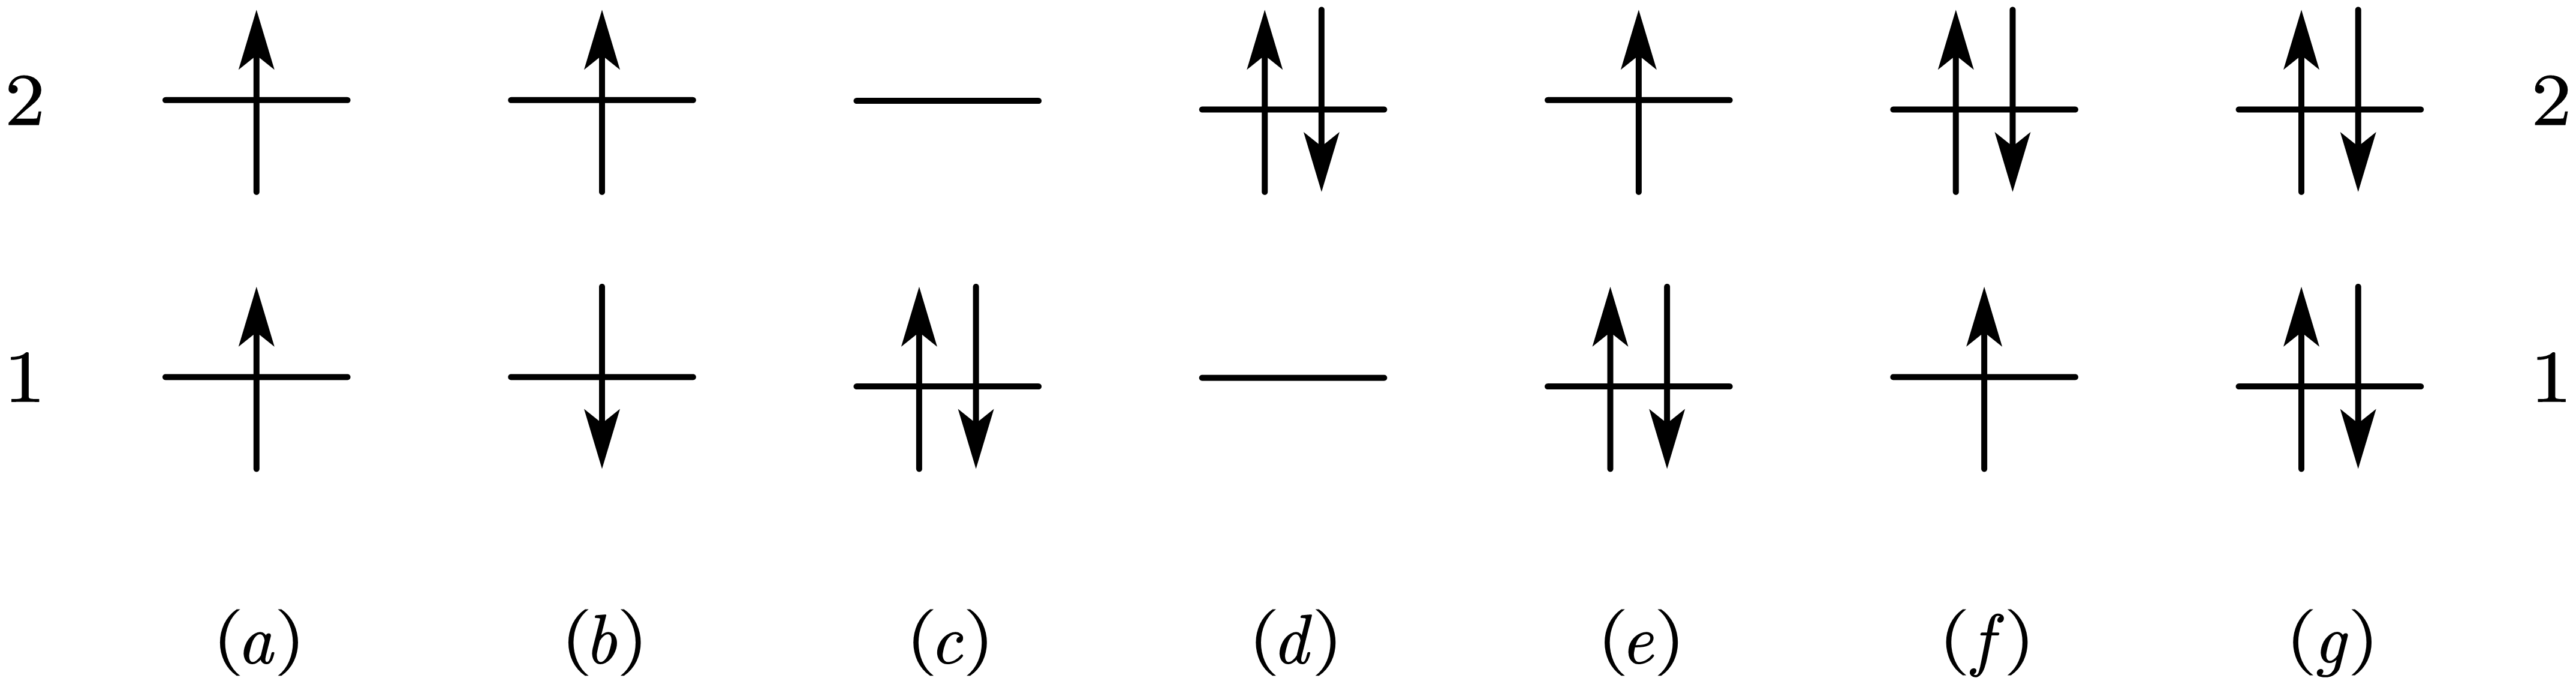
\includegraphics[scale=1.0]{./pictures/2.23/exercise.png}
	\end{center}
	
	\begin{enumerate}
	
	\item[a.] $h_{11} + h_{22} +  J_{12} - K_{12}$.
	
	\item[b.] $h_{11} + h_{22} +  J_{12}$.
	
	\item[c.] $2h_{11} +  J_{11}$.
	
	\item[d.] $2h_{22} +  J_{22}$.
	
	\item[e.] $2h_{11} + h_{22} +  J_{11} + 2J_{12} - K_{12}$.
	
	\item[f.] $2h_{22} + h_{11} +  J_{22} + 2J_{12} - K_{12}$.
	
	\item[g.] $2h_{11} + 2h_{22} +  J_{11} +  J_{22} + 4J_{12} - 2K_{12}$.
	
	\end{enumerate}		
	
	\end{exercise}
	
	\begin{solution}
	
	\begin{itemize}
	
	\item[a.] There are 2 electrons in spatial orbital $1$ and $2$, contributing the terms $h_{11}$ and $h_{22}$. There is only 1 unique pair of electrons in spatial orbitals 1 and 2, contributing the term $J_{12}$. There is only 1 unique pair of electrons with parallel spins in spatial orbitals 1 and 2, contributing the term $-K_{12}$. Thus,
	\[
		E_a = h_{11} + h_{22} +  J_{12} - K_{12}.
	\]
	
	\item[b.] There are 2 electrons in spatial orbital $1$ and $2$, contributing the terms $h_{11}$ and $h_{22}$. There is only 1 unique pair of electrons in spatial orbitals 1 and 2, contributing the term $J_{12}$. However, there is no unique pair of electrons with parallel spins. Thus,
	\[
		E_b = h_{11} + h_{22} +  J_{12} .
	\]
	
	\item[c.] There are 2 electrons both in spatial orbital $1$, contributing the terms $2h_{11}$. There is only 1 unique pair of electrons in spatial orbitals 1, contributing the term $J_{11}$. However, there is no unique pair of electrons with parallel spins. Thus,
	\[
		E_c = 2h_{11} +  J_{11} .
	\]

	\item[d.] There are 2 electrons both in spatial orbital $2$, contributing the terms $2h_{22}$. There is only 1 unique pair of electrons in spatial orbitals 1, contributing the term $J_{22}$. However, there is no unique pair of electrons with parallel spins. Thus,
	\[
		E_d = 2h_{22} +  J_{22} .
	\]
	
	\item[e.] There are 3 electrons in spatial orbital $1$, $1$ and $2$, contributing the terms $h_{11}$, $h_{11}$  and $h_{22}$. There are 3 unique pairs of electrons in spatial orbitals 1 and 1, 1 and 2, 1 and 2, contributing the term $J_{11}$, $J_{12}$ and $J_{12}$. There is only 1 unique pair of electrons with parallel spins in spatial orbitals 1 and 2, contributing the term $-K_{12}$. Thus,
	\[
		E_e = h_{11} + h_{11} + h_{22} + J_{11} + J_{12} + J_{12} - K_{12} = 2h_{11} + h_{22} +  J_{11} + 2J_{12} - K_{12}.
	\]
	
	\item[f.] There are 3 electrons in spatial orbital $1$, $2$ and $2$, contributing the terms $h_{11}$, $h_{22}$  and $h_{22}$. There are 3 unique pairs of electrons in spatial orbitals 1 and 2, 1 and 2, 2 and 2, contributing the term $J_{12}$, $J_{12}$ and $J_{22}$. There is only 1 unique pair of electrons with parallel spins in spatial orbitals 1 and 2, contributing the term $-K_{12}$. Thus,
	\[
		E_f = h_{11} + h_{22} + h_{22} + J_{12} + J_{12} + J_{22} - K_{12} = 2h_{22} + h_{11} +  J_{22} + 2J_{12} - K_{12} .
	\]
	
	\item[g.] There are 4 electrons in spatial orbital $1$, $1$, $2$ and $2$, contributing the terms $h_{11}$, $h_{11}$, $h_{22}$  and $h_{22}$. There are 6 unique pairs of electrons in spatial orbitals 1 and 1, 1 and 2, 1 and 2, 1 and 2, 1 and 2, 2 and 2, contributing the term $J_{11}$, $J_{12}$, $J_{12}$, $J_{12}$, $J_{12}$, and $J_{22}$. There are only 2 unique pair of electrons with parallel spins in spatial orbitals 1 and 2, 1 and 2, contributing the term $-K_{12}$ and $-K_{12}$. Thus,
	\begin{align*}
		E_g &= h_{11} + h_{11} + h_{22} + h_{22} + J_{11} + J_{12} + J_{12} + J_{12} + J_{12} + J_{22} - K_{12} - K_{12} \\
		&= 2h_{11} + 2h_{22} +  J_{11} +  J_{22} + 4J_{12} - 2K_{12} .
	\end{align*}
	
	\end{itemize}		
	
	\end{solution}
	
	\section{Second Quantization}
	
	\subsection{Creation and Annihilation Operators and Their Anticommutation Relations}
	
	% 2.24
	\begin{exercise}
	Show, using the properties of determinants, that
	\[
		( a^\dagger_1 a^\dagger_2 + a^\dagger_2 a^\dagger_1 ) | K \rangle = 0 
	\]
	for every $| K \rangle$ in the set $\{ |\chi_1\chi_2\rangle , |\chi_1\chi_3\rangle , |\chi_1\chi_4\rangle , |\chi_2\chi_3\rangle , |\chi_2\chi_4\rangle , |\chi_3\chi_4\rangle \}$.
	\end{exercise}
	
	\begin{solution}
	
	Using (2.194), the conclusion can be obtained at once.	
	
	\end{solution}
	
	% 2.25
	\begin{exercise}
	Show, using the properties of determinants, that
	\begin{align*}
		( a_1 a^\dagger_2 + a^\dagger_2 a_1 ) | K \rangle &= 0 , \\
		( a_1 a^\dagger_1 + a^\dagger_1 a_1 ) | K \rangle &= | K \rangle
	\end{align*}
	for every $| K \rangle$ in the set $\{ |\chi_1\chi_2\rangle , |\chi_1\chi_3\rangle , |\chi_1\chi_4\rangle , |\chi_2\chi_3\rangle , |\chi_2\chi_4\rangle , |\chi_3\chi_4\rangle \}$.
	\end{exercise}
	
	\begin{solution}
	
	Using (2.217), the conclusion can be obtained at once.
	
	\end{solution}
	
	% 2.26
	\begin{exercise}
	Show using second quantization that $\langle \chi_i | \chi_j \rangle = \delta_{ij}$.
	\end{exercise}
	
	\begin{solution}
	
	The proof is direct.
	\[
		\langle \chi_i | \chi_j \rangle = \langle | a_i a^\dagger_j | \rangle = \langle | \delta_{ij} - a^\dagger_j a_i | \rangle = \delta_{ij} \langle | \rangle - \langle | a^\dagger_j a_i | \rangle = \delta_{ij} .
	\]	
	
	\end{solution}
	
	% 2.27
	\begin{exercise}
	Given a state 
	\[
		| K \rangle = | \chi_1 \chi_2 \cdots \chi_N \rangle = a^\dagger_1 a^\dagger_2 \cdots a^\dagger_N | \rangle,
	\]
	show that $\langle K | a^\dagger_i a_j | K \rangle = 1$ if $i=j$ and $i \in \{ 1 , 2 , \cdots, N \}$, but is zero otherwise.
	\end{exercise}
	
	\begin{solution}
	
	The proof is direct, too.	
	\[
		\langle K | a^\dagger_i a_j | K \rangle = \langle K | \delta_{ij} - a_j a^\dagger_i | K \rangle = \delta_{ij} \langle K | K \rangle - \langle K | a_j a^\dagger_i | K \rangle = \delta_{ij} - \langle K | a_j a^\dagger_i | K \rangle.
	\]	
	It is evident that $\langle K | a^\dagger_i a_j | K \rangle$ will be one if and only if $i=j$ and $i \in \{ 1, 2, \ldots, N \}$. Otherwise, it will be zero.
	
	\end{solution}
	
	% 2.28
	\begin{exercise}
	Let $|\Psi_0\rangle = | \chi_1 \cdots \chi_a \chi_b \cdots \chi_N \rangle$ be the Hartree-Fock ground state wave function. Show that
	\begin{enumerate}
	
	\item[a.] $a_r | \Psi_0 \rangle = 0 = \langle \Psi_0 | a^\dagger_r$.
	
	\item[b.] $a^\dagger_a | \Psi_0 \rangle = 0 = \langle \Psi_0 | a_a$.
	
	\item[c.] $| \Psi^r_a \rangle = a^\dagger_r a_a | \Psi_0 \rangle $.
	
	\item[d.] $\langle \Psi^r_a | = \langle \Psi_0 | a^\dagger_a a_r$.
	
	\item[e.] $| \Psi^{rs}_{ab} \rangle = a^\dagger_s a_b a^\dagger_r a_a | \Psi_0 \rangle = a^\dagger_r a^\dagger_s a_b  a_a | \Psi_0 \rangle $.
	
	\item[f.] $\langle \Psi^{rs}_{ab} | = \langle \Psi_0 | a^\dagger_a a_r a^\dagger_b a_s = \langle \Psi_0 | a^\dagger_a a^\dagger_b a_s a_r$.
	
	\end{enumerate}
	\end{exercise}
	
	\begin{solution}
	
	Assume that $a$, $b$ are labels of occupied spin orbitals while $r$, $s$ are labels of unoccupied spin orbitals.
	
	\begin{itemize}

	\item[a.] It is evident because there exists no electron occupying spin orbital $r$.
	
	\item[b.] It is also evident because there is an electron occupying spin orbital $a$.
	
	\item[c.] The verification is direct.
	\begin{align*}
		 | \Psi^r_a \rangle &= | \chi_1 \cdots \chi_r \chi_b \cdots \chi_N \rangle = - | \chi_r \cdots \chi_1 \chi_b \cdots \chi_N \rangle = - a^\dagger_r | \cdots \chi_1 \chi_b \cdots \chi_N \rangle \\
		 &=  - a^\dagger_r a_a | \chi_a \cdots \chi_1 \chi_b \cdots \chi_N \rangle = a^\dagger_r a_a | \chi_1 \cdots \chi_a \chi_b \cdots \chi_N \rangle = a^\dagger_r a_a | \Psi_0 \rangle .
	\end{align*}
	
	\item[d.] The verification is direct, too.
	\begin{align*}
		\langle \Psi^r_a | &= \langle \chi_1 \cdots \chi_r \chi_b \cdots \chi_N | = - \langle \chi_1 \cdots \chi_N \chi_b \cdots \chi_r | = - \langle \chi_1 \cdots \chi_N \chi_b \cdots | a_r \\
		&= -  \langle \chi_1 \cdots \chi_N \chi_b \cdots \chi_a | a^\dagger_a a_r = \langle \chi_1 \cdots \chi_a \chi_b \cdots \chi_N | a^\dagger_a a_r = \langle \Psi_0 | a^\dagger_a a_r . 
	\end{align*}
	
	
	\item[e.] The verification is direct, too.
	\begin{align*}
		| \Psi^{rs}_{ab} \rangle &= | \chi_1 \chi_2 \cdots \chi_r \chi_s \cdots \chi_N \rangle = (-1)^2 | \chi_r \chi_s \cdots \chi_1 \chi_2 \cdots \chi_N \rangle = a^\dagger_r | \chi_s \cdots \chi_1 \chi_2 \cdots \chi_N \rangle \\
		&= a^\dagger_r a^\dagger_s | \cdots \chi_1 \chi_2 \cdots \chi_N \rangle = a^\dagger_r a^\dagger_s a_b | \chi_b \cdots \chi_1 \chi_2 \cdots \chi_N \rangle = - a^\dagger_r a^\dagger_s a_b | \chi_2 \cdots \chi_1 \chi_b \cdots \chi_N \rangle \\
		&= - a^\dagger_r a^\dagger_s a_b a_a | \chi_a \chi_2 \cdots \chi_1 \chi_b \cdots \chi_N \rangle = a^\dagger_r a^\dagger_s a_b a_a | \chi_1 \chi_2 \cdots \chi_a \chi_b \cdots \chi_N \rangle = a^\dagger_r a^\dagger_s a_b a_a | \Psi_0 \rangle .
	\end{align*}		
	Note that with $\delta_{ar} = \delta_{br} = \delta_{as} = \delta_{bs} = 0$, 
	\[
		a^\dagger_r a^\dagger_s a_b = - a^\dagger_s a^\dagger_r a_b = - a^\dagger_s ( \delta_{br} - a_b a^\dagger_r ) = a^\dagger_s a_b a^\dagger_r .
	\]
	We obtain that
	\[
		| \Psi^{rs}_{ab} \rangle = a^\dagger_r a^\dagger_s a_b a_a | \Psi_0 \rangle = a^\dagger_s a_b a^\dagger_r a_a | \Psi_0 \rangle .
	\]
	
	\item[f.] The verification is direct, too.
	\begin{align*}
		\langle \Psi^{rs}_{ab} | &= \langle \chi_1 \cdots \chi_r \chi_s \cdots \chi_{N-1} \chi_N | = (-1)^2 \langle \chi_1 \cdots \chi_N \chi_{N-1} \cdots \chi_s \chi_r | = \langle \chi_1 \cdots \chi_N \chi_{N-1} \cdots \chi_s | a_r \\
		&= \langle \chi_1 \cdots \chi_N \chi_{N-1} \cdots | a_s a_r = \langle \chi_1 \cdots \chi_N \chi_{N-1} \cdots \chi_b | a^\dagger_b a_s a_r = - \langle \chi_1 \cdots \chi_N \chi_b \cdots \chi_{N-1} | a^\dagger_b a_s a_r \\
		&= - \langle \chi_1 \cdots \chi_N \chi_b \cdots \chi_{N-1} \chi_a | a^\dagger_a a^\dagger_b a_s a_r = \langle \chi_1 \cdots \chi_a \chi_b \cdots \chi_{N-1} \chi_N | a^\dagger_a a^\dagger_b a_s a_r = \langle \Psi_0 | a^\dagger_a a^\dagger_b a_s a_r .
	\end{align*}
	
	In the same way, we can find that
	\[
		a^\dagger_b a_s a_r = - a^\dagger_b a_r a_s = - ( \delta_{br} - a_r a^\dagger_b ) a_s = a_r a^\dagger_b a_s .
	\]	
	Thus, 
	\[
		\langle \Psi^{rs}_{ab} | = \langle \Psi_0 | a^\dagger_a a^\dagger_b a_s a_r = \langle \Psi_0 | a^\dagger_a a_r a^\dagger_b a_s .
	\]
	
	\end{itemize}
	
	\end{solution}
	
	\subsection{Second-Quantized Operators and Their Matrix Elements}
	
	% 2.29
	\begin{exercise}
	Let $| \Psi_0 \rangle = | \chi_1 \chi_2 \rangle = a^\dagger_1 a^\dagger_2 | \rangle$ be the Hartree-Fock wave function for minimal basis $\ce{H2}$. Show using second quantization that
	\[
		\langle \Psi_0 | \mathscr{O}_1 | \Psi_0 \rangle = \sum_{ij} \langle i | h | j \rangle \langle | a_2 a_1 a^\dagger_i a_j a^\dagger_1 a^\dagger_2 | \rangle = \langle 1 | h | 1 \rangle + \langle 2 | h | 2 \rangle.
	\]
	\end{exercise}
	
	\begin{solution}
	
	Using (2.231) and the conclusion of Exercise 2.28, we find that
	\begin{align*}
		&\hspace{1.4em}\langle \Psi_0 | \mathscr{O}_1 | \Psi_0 \rangle = \langle \chi_1 \chi_2 | \sum_{ij} \langle i | h | j \rangle a^\dagger_i a_j | \chi_1 \chi_2 \rangle = \sum_{ij} \langle i | h | j \rangle \langle | a_2 a_1 a^\dagger_i a_j a^\dagger_1 a^\dagger_2 | \rangle \\
		&= \sum_{ij} \langle i | h | j \rangle \langle | a_2 ( \delta_{1i} - a^\dagger_i a_1 ) ( \delta_{j1} - a^\dagger_1 a_j ) a^\dagger_2 | \rangle \\
		&= \sum_{ij} \langle i | h | j \rangle \left[ \delta_{1i} \delta_{1j} \langle | a_2 a^\dagger_2 | \rangle - \delta_{1i} \langle | a_2 a^\dagger_1 a_j a^\dagger_2 | \rangle - \delta_{j1} \langle | a_2 a^\dagger_i a_1 a^\dagger_2 | \rangle + \langle | a_2 a^\dagger_i a_1 a^\dagger_1 a_j a^\dagger_2 | \rangle \right] \\
		&= \langle 1 | h | 1 \rangle \langle | a_2 a^\dagger_2 | \rangle - \sum_j \langle 1 | h | j \rangle \langle | a_2 a^\dagger_1 a_j a^\dagger_2 | \rangle - \sum_i \langle i | h | 1 \rangle \langle | a_2 a^\dagger_i a_1 a^\dagger_2 | \rangle + \sum_{ij} \langle i | h | j \rangle \langle | a_2 a^\dagger_i a_1 a^\dagger_1 a_j a^\dagger_2 | \rangle \\
		&= \langle 1 | h | 1 \rangle \left( \langle | \delta_{22} - a^\dagger_2 a_2 | \rangle \right) - \sum_j \langle 1 | h | j \rangle \langle | ( \delta_{12} - a^\dagger_1 a_2 )  a_j a^\dagger_2 | \rangle - \sum_i \langle i | h | 1 \rangle \langle | a_2 a^\dagger_i ( \delta_{12} - a^\dagger_2 a_1 ) | \rangle \\
		&\hspace{4em} + \sum_{ij} \langle i | h | j \rangle \langle | ( \delta_{2i} - a^\dagger_i a_2 ) a_1 a^\dagger_1 ( \delta_{2j} - a^\dagger_2 a_j ) | \rangle \\
		&= \langle 1 | h | 1 \rangle \left( 1 - 0 \right) + \sum_j \langle 1 | h | j \rangle \langle | a^\dagger_1 a_2 a_j a^\dagger_2 | \rangle + \sum_i \langle i | h | 1 \rangle \langle | a_2 a^\dagger_i a^\dagger_2 a_1 | \rangle \\
		&\hspace{4em} + \sum_{ij} \langle i | h | j \rangle \left[ \delta_{2i} \delta_{2j} \langle | a_1 a^\dagger_1 | \rangle - \delta_{2i} \langle | a_1 a^\dagger_1 a^\dagger_2 a_j | \rangle - \delta_{2j} \langle | a^\dagger_i a_2 a_1 a^\dagger_1 | \rangle + \langle | a^\dagger_i a_2 a_1 a^\dagger_1 a^\dagger_2 a_j | \rangle \right] \\
		&= \langle 1 | h | 1 \rangle + 0 + 0 + \langle 2 | h | 2 \rangle ( \delta_{11} - \langle | a_1 a^\dagger_1 | \rangle ) - 0 - 0 + 0 = \langle 1 | h | 1 \rangle + \langle 2 | h | 2 \rangle ( 1 - 0 ) = \langle 1 | h | 1 \rangle + \langle 2 | h | 2 \rangle.
	\end{align*}		
	
	\end{solution}
	
	% 2.30
	\begin{exercise}
	Show that
	\[
		\langle \Psi^r_a | \mathscr{O}_1 | \Psi_0 \rangle = \sum_{ij} \langle i | h | j \rangle \langle \Psi_0 | a^\dagger_a a_r a^\dagger_i a_j | \Psi_0 \rangle = \langle r | h | a \rangle
	\]
	by moving $a^\dagger_a$ and $a_r$ to the right.
	\end{exercise}
	
	\begin{solution}
	
	Using (2.231) and the conclusion of Exercise 2.28, we find that
	\begin{align*}
		&\hspace{1.4em}\langle \Psi^r_a | \mathscr{O}_1 | \Psi_0 \rangle = \langle \Psi_0 | a^\dagger_a a_r \sum_{ij} \langle i | h | j \rangle a^\dagger_i a_j | \Psi_0 \rangle = \sum_{ij} \langle i | h | j \rangle \langle \Psi_0 | a^\dagger_a a_r a^\dagger_i a_j | \Psi_0 \rangle \\
		&= \sum_{ij} \langle i | h | j \rangle \langle \Psi_0 | a^\dagger_a ( \delta_{ri} - a^\dagger_i a_r ) a_j | \Psi_0 \rangle = \sum_j \langle r | h | j \rangle \langle \Psi_0 | a^\dagger_a a_j | \Psi_0 \rangle - \sum_{ij} \langle i | h | j \rangle \langle \Psi_0 | a^\dagger_a a^\dagger_i a_r a_j | \Psi_0 \rangle \\
		&= \sum_j \langle r | h | j \rangle \langle \Psi_0 | ( \delta_{aj} - a_j a^\dagger_a ) | \Psi_0 \rangle + \sum_{ij} \langle i | h | j \rangle \langle \Psi_0 | a^\dagger_a a^\dagger_i a_j a_r | \Psi_0 \rangle \\
		&= \sum_j \langle r | h | j \rangle \delta_{aj} - \sum_j \langle r | h | j \rangle \langle \Psi_0 | a_j a^\dagger_a | \Psi_0 \rangle + 0 = \langle r | h | a \rangle + 0 = \langle r | h | a \rangle .
	\end{align*}
	
	\end{solution}
	
	% 2.31
	\begin{exercise}
	Show that
	\[
		\langle \Psi^r_a | \mathscr{O}_2 | \Psi_0 \rangle = \sum_b^N \langle rb || ab \rangle .
	\]
	{\it Hint}: first show that
	\begin{align*}
		\langle \Psi_0 | a^\dagger_a a_r a^\dagger_i a^\dagger_j a_l a_k | \Psi_0 \rangle &= \delta_{rj} \delta_{al} \langle \Psi_0 | a^\dagger_i a_k | \Psi_0 \rangle - \delta_{rj} \delta_{ak} \langle \Psi_0 | a^\dagger_i a_l | \Psi_0 \rangle \\
		&\hspace{4em} + \delta_{ri} \delta_{ak} \langle \Psi_0 | a^\dagger_j a_l | \Psi_0 \rangle - \delta_{ri} \delta_{al} \langle \Psi_0 | a^\dagger_j a_k | \Psi_0 \rangle
	\end{align*}
	then refer to Exercise 2.27.
	\end{exercise}
	
	\begin{solution}
	
	Similar to Exercise 2.30, we find that
	\begin{align*}
		&\hspace{1.4em}\langle \Psi_0 | a^\dagger_a a_r a^\dagger_i a^\dagger_j a_l a_k | \Psi_0 \rangle \\
		&= \langle \Psi_0 | a^\dagger_a ( \delta_{ri} - a^\dagger_i a_r ) a^\dagger_j a_l a_k | \Psi_0 \rangle = \delta_{ri} \langle \Psi_0 | a^\dagger_a a^\dagger_j a_l a_k | \Psi_0 \rangle - \langle \Psi_0 | a^\dagger_a a^\dagger_i a_r a^\dagger_j a_l a_k | \Psi_0 \rangle \\
		&= - \delta_{ri} \langle \Psi_0 | a^\dagger_j a^\dagger_a a_l a_k | \Psi_0 \rangle - \langle \Psi_0 | a^\dagger_a a^\dagger_i ( \delta_{rj} - a^\dagger_j a_r ) a_l a_k | \Psi_0 \rangle \\
		&= - \delta_{ri} \langle \Psi_0 | a^\dagger_j ( \delta_{al} - a_l a^\dagger_a ) a_k | \Psi_0 \rangle - \delta_{rj} \langle \Psi_0 | a^\dagger_a a^\dagger_i a_l a_k | \Psi_0 \rangle + \langle \Psi_0 | a^\dagger_a a^\dagger_i a^\dagger_j a_r a_l a_k | \Psi_0 \rangle  \\
		&= - \delta_{ri} \delta_{al} \langle \Psi_0 | a^\dagger_j a_k | \Psi_0 \rangle + \delta_{ri} \langle \Psi_0 | a^\dagger_j a_l a^\dagger_a a_k | \Psi_0 \rangle + \delta_{rj} \langle \Psi_0 | a^\dagger_i a^\dagger_a a_l a_k | \Psi_0 \rangle - \langle \Psi_0 | a^\dagger_a a^\dagger_i a^\dagger_j a_l a_r a_k | \Psi_0 \rangle \\
		&= - \delta_{ri} \delta_{al} \langle \Psi_0 | a^\dagger_j a_k | \Psi_0 \rangle + \delta_{ri} \langle \Psi_0 | a^\dagger_j a_l ( \delta_{ak} - a_k a^\dagger_a ) | \Psi_0 \rangle \\
		&\hspace{4em} + \delta_{rj} \langle \Psi_0 | a^\dagger_i ( \delta_{al} - a_l a^\dagger_a ) a_k | \Psi_0 \rangle + \langle \Psi_0 | a^\dagger_a a^\dagger_i a^\dagger_j a_l a_k a_r | \Psi_0 \rangle \\
		&= - \delta_{ri} \delta_{al} \langle \Psi_0 | a^\dagger_j a_k | \Psi_0 \rangle + \delta_{ri} \delta_{ak} \langle \Psi_0 | a^\dagger_j a_l | \Psi_0 \rangle - \delta_{ri} \langle \Psi_0 | a^\dagger_j a_l a_k a^\dagger_a | \Psi_0 \rangle \\
		&\hspace{4em} + \delta_{rj} \delta_{al} \langle \Psi_0 | a^\dagger_i a_k | \Psi_0 \rangle - \delta_{rj} \langle \Psi_0 | a^\dagger_i a_l a^\dagger_a a_k | \Psi_0 \rangle + 0 \\
		&= - \delta_{ri} \delta_{al} \langle \Psi_0 | a^\dagger_j a_k | \Psi_0 \rangle + \delta_{ri} \delta_{ak} \langle \Psi_0 | a^\dagger_j a_l | \Psi_0 \rangle - 0 + \delta_{rj} \delta_{al} \langle \Psi_0 | a^\dagger_i a_k | \Psi_0 \rangle - \delta_{rj} \langle \Psi_0 | a^\dagger_i a_l ( \delta_{ak} - a_k a^\dagger_a ) | \Psi_0 \rangle \\
		&= - \delta_{ri} \delta_{al} \langle \Psi_0 | a^\dagger_j a_k | \Psi_0 \rangle + \delta_{ri} \delta_{ak} \langle \Psi_0 | a^\dagger_j a_l | \Psi_0 \rangle \\
		&\hspace{4em} + \delta_{rj} \delta_{al} \langle \Psi_0 | a^\dagger_i a_k | \Psi_0 \rangle - \delta_{rj} \delta_{ak} \langle \Psi_0 | a^\dagger_i a_l | \Psi_0 \rangle + \delta_{rj} \langle \Psi_0 | a^\dagger_i a_l a_k a^\dagger_a | \Psi_0 \rangle  \\
		&= \delta_{rj} \delta_{al} \langle \Psi_0 | a^\dagger_i a_k | \Psi_0 \rangle - \delta_{rj} \delta_{ak} \langle \Psi_0 | a^\dagger_i a_l | \Psi_0 \rangle + \delta_{ri} \delta_{ak} \langle \Psi_0 | a^\dagger_j a_l | \Psi_0 \rangle - \delta_{ri} \delta_{al} \langle \Psi_0 | a^\dagger_j a_k | \Psi_0 \rangle .
	\end{align*}
	
	Note that $\langle \Psi_0 | a^\dagger_i a_j | \Psi_0 \rangle$ equals 1 if and only if $i$ and $j$ is should be labels of occupied spin orbitals like $a$ and $b$. Hence, we find that
	\begin{align*}
		&\hspace{1.4em}\langle \Psi^r_a | \mathscr{O}_2 | \Psi_0 \rangle = \langle \Psi_0 | a^\dagger_a a_r \frac{1}{2}\sum_{ijkl} \langle ij | kl \rangle a^\dagger_i a^\dagger_j a_l a_k | \Psi_0 \rangle = \frac{1}{2} \sum_{ijkl} \langle ij | kl \rangle \langle \Psi_0 | a^\dagger_a a_r a^\dagger_i a^\dagger_j a_l a_k  | \Psi_0 \rangle \\
		&= \frac{1}{2} \sum_{ijkl} \langle ij | kl \rangle ( \delta_{rj} \delta_{al} \langle \Psi_0 | a^\dagger_i a_k | \Psi_0 \rangle - \delta_{rj} \delta_{ak} \langle \Psi_0 | a^\dagger_i a_l | \Psi_0 \rangle + \delta_{ri} \delta_{ak} \langle \Psi_0 | a^\dagger_j a_l | \Psi_0 \rangle - \delta_{ri} \delta_{al} \langle \Psi_0 | a^\dagger_j a_k | \Psi_0 \rangle ) \\
		&= \frac{1}{2} \sum_{ik} \langle ir | ka \rangle \langle \Psi_0 | a^\dagger_i a_k | \Psi_0 \rangle - \frac{1}{2} \sum_{il} \langle ir | al \rangle \langle \Psi_0 | a^\dagger_i a_l | \Psi_0 \rangle \\
		&\hspace{4em} + \frac{1}{2} \sum_{jl} \langle rj | al \rangle \langle \Psi_0 | a^\dagger_j a_l | \Psi_0 \rangle - \frac{1}{2} \sum_{jk} \langle rj | ka \rangle \langle \Psi_0 | a^\dagger_j a_k | \Psi_0 \rangle \\
		&= \frac{1}{2} \sum_{ij} \langle ir | ja \rangle \langle \Psi_0 | a^\dagger_i a_j | \Psi_0 \rangle - \frac{1}{2} \sum_{ij} \langle ir | aj \rangle \langle \Psi_0 | a^\dagger_i a_j | \Psi_0 \rangle \\
		&\hspace{4em} + \frac{1}{2} \sum_{ij} \langle ri | aj \rangle \langle \Psi_0 | a^\dagger_i a_j | \Psi_0 \rangle - \frac{1}{2} \sum_{ij} \langle ri | ja \rangle \langle \Psi_0 | a^\dagger_i a_j | \Psi_0 \rangle \\
		&= \sum_{ij} \langle ir | ja \rangle \langle \Psi_0 | a^\dagger_i a_j | \Psi_0 \rangle - \langle ir | aj \rangle \langle \Psi_0 | a^\dagger_i a_j | \Psi_0 \rangle = \sum_{ij} \langle ir || ja \rangle \langle \Psi_0 | a^\dagger_i a_j | \Psi_0 \rangle \\
		&= \sum_{ij} \langle ri || aj \rangle \langle \Psi_0 | a^\dagger_i a_j | \Psi_0 \rangle = \sum_b^N \langle rb || ab \rangle .
	\end{align*}
	
	\end{solution}
	
	\section{Spin-Adapted Configurations}
	
	\subsection{Spin Operators}
	
	% 2.32
	\begin{exercise}
	a) Derive (2.247) from (2.245); b) Derive (2.248).
	\end{exercise}
	
	\begin{solution}
	
	\begin{itemize}
	
	\item[a)] Using (2.246a) and (2.245c,d), we find that
	\begin{align*}
		s_+ | \alpha \rangle &= ( s_x + i s_y ) | \alpha \rangle = s_x | \alpha \rangle + i s_y | \alpha \rangle = \frac{1}{2} | \beta \rangle + i \times \frac{ i }{ 2 } | \beta \rangle = \left( \frac{1}{2} + i \times \frac{ i }{ 2 } \right) | \beta \rangle = 0 , \\
		s_+ | \beta \rangle &= ( s_x + i s_y ) | \beta \rangle = s_x | \beta \rangle + i s_y | \beta \rangle = \frac{1}{2} | \alpha \rangle + i \times \frac{ -i }{ 2 } | \alpha \rangle = \left( \frac{1}{2} + i \times \frac{ -i }{ 2 } \right) | \alpha \rangle = | \alpha \rangle , \\
		s_- | \alpha \rangle &= ( s_x - i s_y ) | \alpha \rangle = s_x | \alpha \rangle - i s_y | \alpha \rangle = \frac{1}{2} | \beta \rangle - i \times \frac{ i }{ 2 } | \beta \rangle = \left( \frac{1}{2} - i \times \frac{ i }{ 2 } \right) | \beta \rangle = | \beta \rangle , \\
		s_- | \beta \rangle &= ( s_x - i s_y ) | \beta \rangle = s_x | \beta \rangle - i s_y | \beta \rangle = \frac{1}{2} | \alpha \rangle - i \times \frac{ -i }{ 2 } | \alpha \rangle = \left( \frac{1}{2} - i \times \frac{ -i }{ 2 } \right) | \alpha \rangle = 0 .
	\end{align*}
	
	\item[b)] From (2.246a,b) and the conclusion of Exercise 1.4(f), we know that
	\[
		\begin{pmatrix}
			s_+ \\ s_- 
		\end{pmatrix} = \begin{pmatrix}
			1 & i \\
			1 & -i
		\end{pmatrix} \begin{pmatrix}
			s_x \\ s_y
		\end{pmatrix} \Leftrightarrow \begin{pmatrix}
			s_x \\ s_y
		\end{pmatrix} = \begin{pmatrix}
			1 & i \\
			1 & -i
		\end{pmatrix}^{-1} \begin{pmatrix} 
			s_+ \\ s_- 
		\end{pmatrix} = \frac{1}{-2i} \begin{pmatrix}
			-i & -i \\
			-1 & 1
		\end{pmatrix} \begin{pmatrix} 
			s_+ \\ s_- 
		\end{pmatrix} .
	\]
	In other words, we know that
	\[
		s_x = \frac{ -i s_+ -i s_- }{-2i} = \frac{ s_+ + s_- }{2} , \quad s_y = \frac{ - s_+ + s_- }{-2i} = \frac{ s_+ - s_- }{2i} .
	\]
	Besides, with (2.242), it is evident that
	\[
		[ s_+ , s_- ] = [ s_x + i s_y , s_x - i s_y ] = [ s_x , s_x ] - i [ s_x , s_y ] + i [ s_y , s_x ] + [ s_y , s_y ] = -2i [ s_x , s_y ] = -2i ( is_z ) = 2 s_z .
	\]
	
	From (2.241), we find that
	\begin{align*}
		s^2 &= s^2_x + s^2_y + s^2_z = \left( \frac{ s_+ + s_- }{2} \right)^2 + \left( \frac{ s_+ - s_- }{2i} \right)^2 + s^2_z \\
		&= \frac{1}{4} \left( s^2_+ + s_+ s_- + s_- s_+ + s^2_- \right) - \frac{1}{4} \left( s^2_+ - s_+ s_- - s_- s_+ + s^2_- \right) + s^2_z \\
		&= \frac{1}{2} \left( s_+ s_- + s_- s_+ \right) + s^2_z = s_+ s_- + \frac{1}{2} \left( s_- s_+ -  s_+ s_- \right) + s^2_z = s_- s_+ + \frac{1}{2} \left( s_+ s_- -  s_- s_+ \right) + s^2_z \\
		&= s_+ s_- + \frac{1}{2} [ s_- , s_+ ] + s^2_z = s_+ s_- - \frac{1}{2} [ s_+ , s_- ] + s^2_z = s_+ s_- - \frac{1}{2} (2s_z) + s^2_z =  s_+ s_- - s_z + s^2_z \\
		&= s_- s_+ + \frac{1}{2} [ s_+ , s_- ] + s^2_z = s_- s_+ + \frac{1}{2}(2s_z) + s^2_z =  s_- s_+ + s_z + s^2_z .
	\end{align*}

	\end{itemize}		
	
	\end{solution}
	
	% 2.33
	\begin{exercise}
	Find the $2 \times 2$ matrix representations of $s^2$, $s_z$, $s_+$, and $s_-$ in the basis $|\alpha\rangle$, $|\beta\rangle$. Verify the identities analogous to (2.248a,b) for these matrix representations.
	\end{exercise}
	
	\begin{solution}
	
	From (2.245a,b,c,d), at once we get that
	\begin{align*}
		s^2 ( | \alpha \rangle , | \beta \rangle ) &= ( | \alpha \rangle , | \beta \rangle )	\begin{pmatrix}
		\frac{3}{4} & 0 \\ 0 & \frac{3}{4}
		\end{pmatrix} , \\
		s_z ( | \alpha \rangle , | \beta \rangle ) &= ( | \alpha \rangle , | \beta \rangle )	\begin{pmatrix}
		\frac{1}{2} & 0 \\ 0 & -\frac{1}{2}
		\end{pmatrix} , \\
		s_x ( | \alpha \rangle , | \beta \rangle ) &= ( | \alpha \rangle , | \beta \rangle )	\begin{pmatrix}
		0 & \frac{1}{2} \\ \frac{1}{2} & 0
		\end{pmatrix} , \\
		s_y ( | \alpha \rangle , | \beta \rangle ) &= ( | \alpha \rangle , | \beta \rangle )	\begin{pmatrix}
		0 & -\frac{i}{2} \\ \frac{i}{2} & 0
		\end{pmatrix} .
	\end{align*}
	Thus, we find that
	\begin{align*}
		s_+ ( | \alpha \rangle , | \beta \rangle ) &= ( s_x + i s_y ) ( | \alpha \rangle , | \beta \rangle ) = s_x ( | \alpha \rangle , | \beta \rangle ) + i s_y ( | \alpha \rangle , | \beta \rangle ) \\
		&= ( | \alpha \rangle , | \beta \rangle )	\begin{pmatrix}
		0 & \frac{1}{2} \\ \frac{1}{2} & 0
		\end{pmatrix} + ( | \alpha \rangle , | \beta \rangle )	\left[ i \begin{pmatrix}
		0 & -\frac{i}{2} \\ \frac{i}{2} & 0
		\end{pmatrix} \right] = ( | \alpha \rangle , | \beta \rangle )	\begin{pmatrix}
		0 & 1 \\ 0 & 0
		\end{pmatrix} . \\
		s_- ( | \alpha \rangle , | \beta \rangle ) &= ( s_x - i s_y ) ( | \alpha \rangle , | \beta \rangle ) = s_x ( | \alpha \rangle , | \beta \rangle ) - i s_y ( | \alpha \rangle , | \beta \rangle ) \\
		&= ( | \alpha \rangle , | \beta \rangle )	\begin{pmatrix}
		0 & \frac{1}{2} \\ \frac{1}{2} & 0
		\end{pmatrix} + ( | \alpha \rangle , | \beta \rangle )	\left[ -i \begin{pmatrix}
		0 & -\frac{i}{2} \\ \frac{i}{2} & 0
		\end{pmatrix} \right] = ( | \alpha \rangle , | \beta \rangle )	\begin{pmatrix}
		0 & 0 \\ 1 & 0
		\end{pmatrix} .
	\end{align*}
	Thus, in the basis $|\alpha\rangle$, $|\beta\rangle$, the $2 \times 2$ matrix representations of $s^2$, $s_z$, $s_+$ and $s_-$ are
	\begin{sequation}
		s^2 = \begin{pmatrix}
		\frac{3}{4} & 0 \\ 0 & \frac{3}{4}
		\end{pmatrix} , \quad 
		s_z = \begin{pmatrix}
		\frac{1}{2} & 0 \\ 0 & -\frac{1}{2}
		\end{pmatrix} , \quad 
		s_+ = \begin{pmatrix}
		0 & 1 \\ 0 & 0
		\end{pmatrix} , \quad 
		s_- = \begin{pmatrix}
		0 & 0 \\ 1 & 0
		\end{pmatrix} .
	\end{sequation}
	
	Readers can verify that these matrices represent identities similar to (2.248a,b) by themselves.
	
	\end{solution}
	
	% 2.34
	\begin{exercise}
	Using the commutation relations (2.242), show that $[s^2, s_z] = 0$.
	\end{exercise}
	
	\begin{solution}
	
	Before verification, note that for any operators (matrices) $A$, $B$, $C$,
	\begin{align*}
		[AB,C] &= ABC - CAB = ABC - ACB + ACB - CAB \\
		&= A( BC - CB ) + ( AC - CA )B = A[B,C] + [A,C]B.
	\end{align*}

	From (2.241) and (2.242), we find that
	\begin{align*}
		[s^2, s_z] &= [ s^2_x + s^2_y + s^2_z , s_z ] = [ s^2_x , s_z ] + [ s^2_y , s_z ] + [ s^2_z , s_z ] \\
		&= s_x [ s_x , s_z ] + [ s_x , s_z ] s_x + s_y [ s_y , s_z ] + [ s_y , s_z ] s_y + s_z [ s_z , s_z ] + [ s_z , s_z ] s_z \\
		&= - s_x [ s_z , s_x ] - [ s_z , s_x ] s_x + s_y [ s_y , s_z ] + [ s_y , s_z ] s_y + 0 + 0 \\
		&= - s_x ( i s_y ) - ( i s_y ) s_x + s_y ( i s_x ) + ( i s_x ) s_y = ( -i + i ) s_x s_y + ( -i + i ) s_y s_x = 0.
	\end{align*}

	\end{solution}
	
	% 2.35
	\begin{exercise}
	Consider an operator $\mathscr{A}$ that commutes with the Hamiltonian. Suppose $|\Phi\rangle$ is an eigenfunction of $\mathscr{H}$ with eigenvalue $E$. Show that $\mathscr{A}|\Phi\rangle$ is also an eigenfunction of $\mathscr{H}$ with eigenvalue $E$. Thus if $|\Phi\rangle$ is (energetically) nondegenerate, then $\mathscr{A}|\Phi\rangle$ is at most a constant multiple of $|\Phi\rangle$ (i.e., $\mathscr{A}|\Phi\rangle = a|\Phi\rangle$) and hence $|\Phi\rangle$ is an eigenfunction of $\mathscr{A}$. In case of degeneracies, we can always construct appropriate linear combinations of the degenerate eigenfunctions of $\mathscr{H}$ that are also eigenfunctions of $\mathscr{A}$.
	\end{exercise}
	
	\begin{solution}
	
	The proof of that if an operator $\mathscr{A}$ that commutes with the Hamiltonian and $|\Phi\rangle$ is an eigenfunction of $\mathscr{H}$ with eigenvalue $E$, $\mathscr{A}|\Phi\rangle$ will be also an eigenfunction of $\mathscr{H}$ with eigenvalue $E$, is easy.
	\[
		\mathscr{H} \mathscr{A} |\Phi\rangle = \mathscr{A} \mathscr{H} |\Phi\rangle = \mathscr{A} E |\Phi\rangle = E \mathscr{A} |\Phi\rangle .
	\]
	
	\end{solution}
	
	% 2.36
	\begin{exercise}
	Given two nondegenerate eigenfunctions of a hermitian operator $\mathscr{A}$ that commutes with $\mathscr{H}$, i.e., $\mathscr{A} | \Psi_1 \rangle = a_1 | \Psi_1 \rangle$, $\mathscr{A} | \Psi_2 \rangle = a_2 | \Psi_2 \rangle$, $a_1 \neq a_2$, show that $\langle \Psi_1 | \mathscr{H} | \Psi_2 \rangle = 0$. Thus the matrix element of the Hamiltonian between, say, singlet and triplet spin-adapted configurations is zero.
	\end{exercise}
	
	\begin{solution}
	
	As $\mathscr{A}$ is a hermitian operator, $a_1$ and $a_2$ are real and
	\[
		\langle \Psi_2 | \mathscr{A} = a_2 \langle \Psi_2 |.
	\]
	Hence, 
	\[
		a_1 \langle \Psi_2 | \mathscr{H} | \Psi_1 \rangle = \langle \Psi_2 | \mathscr{H} a_1 | \Psi_1 \rangle = \langle \Psi_2 | \mathscr{H} \mathscr{A} | \Psi_1 \rangle = \langle \Psi_2 | \mathscr{A} \mathscr{H} | \Psi_1 \rangle = a_2 \langle \Psi_2 | \mathscr{H} | \Psi_1 \rangle .
	\]
	In other words,
	\[
		( a_1 - a_2 ) \langle \Psi_2 | \mathscr{H} | \Psi_1 \rangle = 0 .
	\]
	Due to $a_1 \neq a_2$, we find that
	\[
		\langle \Psi_1 | \mathscr{H} | \Psi_2 \rangle = 0 .
	\]

	\end{solution}
	
	% 2.37
	\begin{exercise}
	Prove Eq.(2.254). {\it Hint:} Use expansion (2.115) for a Slater determinant and note that $\mathscr{S}_z$, since it is invariant to any permutation of the electron labels, commutes with $\mathscr{P}_n$.
	\end{exercise}
	
	\begin{solution}
	
	Firstly, note that
	\begin{align*}
		s_z(i) \chi_j( \bfx_i ) = \frac{ \delta_{j\alpha} - \delta_{j\beta} }{2} \chi_j( \bfx_i ) .
	\end{align*}
	
	The derivation is exactly the same as that of Exercise 2.15 if $h(i)$ is replaced by $s_z(i)$. And thus, $\sum_{ i=1 }^N \varepsilon_i$ should be replaced by
	\[
		\sum_{ i=1 }^N \frac{ \delta_{j\alpha} - \delta_{j\beta} }{2} = \frac{ N^\alpha - N^\beta }{2} .
	\]
	
	\end{solution}
	
	\subsection{Restricted Determinants and Spin-Adapted Configurations}
	
	% 2.38
	\begin{exercise}
	Prove Eq.(2.256). {\it Hints}: 1) $\mathscr{S}^2 = \mathscr{S}_- \mathscr{S}_+ + \mathscr{S}_z + \mathscr{S}^2_z$,  2) as a result of Eq.(2.254) it is sufficient to show $\mathscr{S}_+ | \psi_i \bar{\psi}_i \cdots \rangle$ = 0, 3) use expansion (2.115) for the determinant, and note the $\mathscr{S}_+$ commutes with the permutation operator, 4) $s_+ \psi_\alpha $ = 0, 5) finally, $s_+ \psi_\beta = \psi_\alpha $, but the determinant vanishes because it has two identical columns.
	\end{exercise}
	
	\begin{solution}
	
%	Firstly, we verify (2.251). Similar to Exercise 2.32, we know that from 
%	\[
%		\mathscr{S}_+ = \mathscr{S}_x + i \mathscr{S}_y , \quad \mathscr{S}_- = \mathscr{S}_x - i \mathscr{S}_y ,
%	\]
%	we can obtain that
%	\[
%		\mathscr{S}_x = \frac{ \mathscr{S}_+ + \mathscr{S}_- }{2}, \quad \mathscr{S}_y = \frac{ \mathscr{S}_+ - \mathscr{S}_- }{2i} ,
%	\]
%	and
%	\[
%		[ \mathscr{S}_+ , \mathscr{S}_- ] = [ \mathscr{S}_x + i \mathscr{S}_y , \mathscr{S}_x - i \mathscr{S}_y ] = - 2i [ \mathscr{S}_x , \mathscr{S}_y ] .
%	\]
%	Here, note that if $j \neq i$, $[ s_x(i) , s_y(j) ]$ will vanish, and thus
%	\[
%		[ \mathscr{S}_x , \mathscr{S}_y ] = \left[ \sum_{ i=1 }^N s_x(i) , \sum_{ j=1 }^N s_y(j) \right] = \sum_{ i=1 }^N \sum_{ j=1 }^N [ s_x(i) , s_y(j) ] = \sum_{ i=1 }^N [ s_x(i) , s_y(i) ] =  \sum_{ i=1 }^N i s_z(i) = i \mathscr{S}_z .
%	\]
%	Using this conclusion, we find that
%	\[
%		[ \mathscr{S}_+ , \mathscr{S}_- ] = - 2i [ \mathscr{S}_x , \mathscr{S}_y ] = -2i \times i \mathscr{S}_z = 2 \mathscr{S}_z .
%	\]
	Firstly, we verify (2.251). Similar to Exercise 2.32, we find that
	\begin{align*}
		\mathscr{S}^2 &= \sum_{ i=1 }^N \sum_{ j=1 }^N \vec{s}(i) \cdot \vec{s}(j) = \sum_{ i=1 }^N \sum_{ j=1 }^N s_x(i) s_x(j) +  s_y(i) s_y(j) + s_z(i) s_z(j) \\
		&= \sum_{ i=1 }^N \sum_{ j=1 }^N \left( \frac{ s_+(i) + s_-(i) }{2} \right) \left( \frac{ s_+(j) + s_-(j) }{2} \right) + \left( \frac{ s_+(i) - s_-(i) }{2i} \right) \left( \frac{ s_+(j) - s_-(j) }{2i} \right) + s_z(i) s_z(j) \\
		&= \sum_{ i=1 }^N \sum_{ j=1 }^N \frac{1}{4} \left[ s_+(i) s_+(j) + s_+(i) s_-(j) + s_-(i) s_+(j) + s_-(i) s_-(j) \right] \\
		&\hspace{6em} - \frac{1}{4} \left[ s_+(i) s_+(j) - s_+(i) s_-(j) - s_-(i) s_+(j) + s_-(i) s_-(j) \right] + s_z(i) s_z(j) \\
		&= \sum_{ i=1 }^N \sum_{ j=1 }^N \frac{1}{2} \left[ s_+(i) s_-(j) + s_-(i) s_+(j) \right] + s_z(i) s_z(j) \\
		&= \sum_{ i=1 }^N \sum_{ j=1 }^N s_+(i) s_-(j) + \frac{1}{2} \left[ s_-(i) s_+(j) - s_+(i) s_-(j) \right] + s_z(i) s_z(j) \\
		&= \sum_{ i=1 }^N \sum_{ j=1 }^N s_-(i) s_+(j) + \frac{1}{2} \left[ s_+(i) s_-(j) - s_-(i) s_+(j) \right] + s_z(i) s_z(j) .
	\end{align*}
	
	The first result can be further simplified to
	\begin{align*}
		&\hspace{1.4em}\sum_{ i=1 }^N \sum_{ j=1 }^N s_+(i) s_-(j) + \frac{1}{2} \left[ s_-(i) s_+(j) - s_+(i) s_-(j) \right] + s_z(i) s_z(j) \\
		&= \sum_{ i=1 }^N s_+(i) \sum_{ j=1 }^N s_-(j) + \frac{1}{2} \sum_{ i=1 }^N \sum_{ j=1 }^N s_-(i) s_+(j) - \frac{1}{2} \sum_{ i=1 }^N \sum_{ j=1 }^N s_+(i) s_-(j) + \sum_{ i=1 }^N \sum_{ j=1 }^N s_z(i) s_z(j) \\
		&= \sum_{ i=1 }^N s_+(i) \sum_{ j=1 }^N s_-(j) + \frac{1}{2} \sum_{ i=1 }^N \sum_{ j=1 }^N [ s_-(i) , s_+(j) ] + s_+(j) s_-(i) - \frac{1}{2} \sum_{ i=1 }^N \sum_{ j=1 }^N s_+(j) s_-(i) + \sum_{ i=1 }^N \sum_{ j=1 }^N s_z(i) s_z(j) \\
		&= \sum_{ i=1 }^N s_+(i) \sum_{ j=1 }^N s_-(j) + \frac{1}{2} \sum_{ i=1 }^N [ s_-(i) , s_+(i) ] + \frac{1}{2} \sum_{ i=1 }^N \sum_{ \substack{ j=1 \\ j \neq i } }^N [ s_-(i) , s_+(j) ] \\
		&\hspace{6em} + \frac{1}{2} \sum_{ i=1 }^N \sum_{ j=1 }^N s_+(j) s_-(i) - \frac{1}{2} \sum_{ i=1 }^N \sum_{ j=1 }^N s_+(j) s_-(i) + \sum_{ i=1 }^N \sum_{ j=1 }^N s_z(i) s_z(j) \\
		&= \sum_{ i=1 }^N s_+(i) \sum_{ j=1 }^N s_-(j) + \frac{1}{2} \sum_{ i=1 }^N -2s_z(i) + 0 + \sum_{ i=1 }^N \sum_{ j=1 }^N s_z(i) s_z(j) \\
		&= \sum_{ i=1 }^N s_+(i) \sum_{ j=1 }^N s_-(j) - \sum_{ i=1 }^N s_z(i) + \sum_{ i=1 }^N s_z(i) \sum_{ j=1 }^N s_z(j) \\
		&= \mathscr{S}_+ \mathscr{S}_- - \mathscr{S}_z + \mathscr{S}_z^2 .
	\end{align*}
	Thus,
	\begin{sequation}
		\mathscr{S}^2 = \mathscr{S}_+ \mathscr{S}_- - \mathscr{S}_z + \mathscr{S}_z^2 .
	\end{sequation}
	
	The second result can be further simplified to
	\begin{align*}
		&\hspace{1.4em}\sum_{ i=1 }^N \sum_{ j=1 }^N s_-(i) s_+(j) + \frac{1}{2} \left[ s_+(i) s_-(j) - s_-(i) s_+(j) \right] + s_z(i) s_z(j)  \\
		&= \sum_{ i=1 }^N s_-(i) \sum_{ j=1 }^N s_+(j) + \frac{1}{2} \sum_{ i=1 }^N \sum_{ j=1 }^N s_+(i) s_-(j) - \frac{1}{2} \sum_{ i=1 }^N \sum_{ j=1 }^N s_-(i) s_+(j) + \sum_{ i=1 }^N \sum_{ j=1 }^N s_z(i) s_z(j) \\
		&= \sum_{ i=1 }^N s_-(i) \sum_{ j=1 }^N s_+(j) + \frac{1}{2} \sum_{ i=1 }^N \sum_{ j=1 }^N [ s_+(i) , s_-(j) ] + s_-(j) s_+(i) - \frac{1}{2} \sum_{ i=1 }^N \sum_{ j=1 }^N s_-(j) s_+(i) + \sum_{ i=1 }^N \sum_{ j=1 }^N s_z(i) s_z(j) \\
		&= \sum_{ i=1 }^N s_-(i) \sum_{ j=1 }^N s_+(j) + \frac{1}{2} \sum_{ i=1 }^N [ s_+(i) , s_-(i) ] + \frac{1}{2} \sum_{ i=1 }^N \sum_{ \substack{ j=1 \\ j \neq i } }^N [ s_+(i) , s_-(j) ] \\
		&\hspace{6em} + \frac{1}{2} \sum_{ i=1 }^N \sum_{ j=1 }^N s_-(j) s_+(i) - \frac{1}{2} \sum_{ i=1 }^N \sum_{ j=1 }^N s_-(j) s_+(i) + \sum_{ i=1 }^N \sum_{ j=1 }^N s_z(i) s_z(j) \\
		&= \sum_{ i=1 }^N s_-(i) \sum_{ j=1 }^N s_+(j) + \frac{1}{2} \sum_{ i=1 }^N 2s_z(i) + 0 + \sum_{ i=1 }^N \sum_{ j=1 }^N s_z(i) s_z(j) \\
		&= \sum_{ i=1 }^N s_-(i) \sum_{ j=1 }^N s_+(j) + \sum_{ i=1 }^N s_z(i) + \sum_{ i=1 }^N s_z(i) \sum_{ j=1 }^N s_z(j) \\
		&= \mathscr{S}_- \mathscr{S}_+ + \mathscr{S}_z + \mathscr{S}_z^2 .
	\end{align*}
	Thus,
	\begin{sequation}
		\mathscr{S}^2 = \mathscr{S}_- \mathscr{S}_+ + \mathscr{S}_z + \mathscr{S}_z^2 .
	\end{sequation}
	
	Secondly, we find that with $N=2n$,
	\begin{align*}
		\mathscr{S}_+ | \psi_1 \bar{\psi}_1 \cdots \psi_n \bar{\psi}_n \rangle &= \sum_{ i=1 }^{ 2n } s_+(i) | \psi_1 \bar{\psi}_1 \cdots \psi_n \bar{\psi}_n \rangle \\
		&= \sum_{ i=1 }^{ n } s_+(2i-1) | \psi_1 \bar{\psi}_1 \cdots \psi_n \bar{\psi}_n \rangle + \sum_{ i=1 }^{ n } s_+(2i) | \psi_1 \bar{\psi}_1 \cdots \psi_n \bar{\psi}_n \rangle .
	\end{align*}
	Note that
	\begin{align*}
		&\hspace{1.4em}s_+(2i-1) | \psi_1 \bar{\psi}_1 \cdots \psi_n \bar{\psi}_n \rangle \\
		&= s_+(2i-1) \frac{1}{ \sqrt{N!} } \sum_{ k } (-1)^k \mathscr{P}_k \psi_1(1) \bar{\psi}_1(2) \cdots \psi_j( 2i-1 ) \bar{\psi}_{j}( 2i ) \cdots \psi_l( 2n - 1 ) \bar{\psi}_l (2n) \\
		&= \frac{1}{ \sqrt{N!} } \sum_{ k } (-1)^k \mathscr{P}_k \psi_1(1) \bar{\psi}_1(2) \cdots \left[ s_+(2i-1) \psi_j( 2i-1 ) \right] \bar{\psi}_{j}( 2i ) \cdots \psi_l( 2n - 1 ) \bar{\psi}_l (2n) \\
		&= \frac{1}{ \sqrt{N!} } \sum_{ k } (-1)^k \mathscr{P}_k \psi_1(1) \bar{\psi}_1(2) \cdots 0 \bar{\psi}_{j}( 2i ) \cdots \psi_l( 2n - 1 ) \bar{\psi}_l (2n) = 0, \\
		&\hspace{1.4em}s_+(2i) | \psi_1 \bar{\psi}_1 \cdots \psi_n \bar{\psi}_n \rangle \\
		&= s_+(2i) \frac{1}{ \sqrt{N!} } \sum_{ k } (-1)^k \mathscr{P}_k \psi_1(1) \bar{\psi}_1(2) \cdots \psi_j( 2i-1 ) \bar{\psi}_{j}( 2i ) \cdots \psi_l( 2n - 1 ) \bar{\psi}_l (2n) \\
		&= \frac{1}{ \sqrt{N!} } \sum_{ k } (-1)^k \mathscr{P}_k \psi_1(1) \bar{\psi}_1(2) \cdots \psi_j( 2i-1 ) \left[ s_+(2i) \bar{\psi}_{j}( 2i ) \right] \cdots \psi_l( 2n - 1 ) \bar{\psi}_l (2n) \\
		&= \frac{1}{ \sqrt{N!} } \sum_{ k } (-1)^k \mathscr{P}_k \psi_1(1) \bar{\psi}_1(2) \cdots \psi_j( 2i-1 ) \psi_{j}( 2i ) \cdots \psi_l( 2n - 1 ) \bar{\psi}_l (2n) \\
		&= | \psi_1 \bar{\psi}_1 \cdots \psi_j \psi_j \psi_n \bar{\psi}_n \rangle = 0 .
	\end{align*}		
	
	Thus,
	\[
		\mathscr{S}_+ | \psi_1 \bar{\psi}_1 \cdots \psi_n \bar{\psi}_n \rangle = \sum_{ i=1 }^{ n } s_+(2i-1) | \psi_1 \bar{\psi}_1 \cdots \psi_n \bar{\psi}_n \rangle + \sum_{ i=1 }^{ n } s_+(2i) | \psi_1 \bar{\psi}_1 \cdots \psi_n \bar{\psi}_n \rangle = 0 + 0 = 0 ,
	\]	
	and	using (2.254),
	\begin{align*}
		\mathscr{S}^2 | \psi_1 \bar{\psi}_1 \cdots \psi_n \bar{\psi}_n \rangle &= ( \mathscr{S}_- \mathscr{S}_+ + \mathscr{S}_z + \mathscr{S}_z^2 ) | \psi_1 \bar{\psi}_1 \cdots \psi_n \bar{\psi}_n \rangle \\
		&= \mathscr{S}_- \mathscr{S}_+ | \psi_1 \bar{\psi}_1 \cdots \psi_n \bar{\psi}_n \rangle + \mathscr{S}_z | \psi_1 \bar{\psi}_1 \cdots \psi_n \bar{\psi}_n \rangle + \mathscr{S}_z \mathscr{S}_z | \psi_1 \bar{\psi}_1 \cdots \psi_n \bar{\psi}_n \rangle =  0 .
	\end{align*}
	
	In conclusion, (2.256) has been proved.
	
	\end{solution}
	
	% 2.39
	\begin{exercise}
	Using $\mathscr{S}^2 = \mathscr{S}_- \mathscr{S}_+ + \mathscr{S}_z + \mathscr{S}^2_z$, show that $|{}^1 \Psi^2_1 \rangle$ is a singlet while $|{}^3 \Psi^2_1 \rangle$, $| \Psi^{\bar 2}_1 \rangle$ and $| \Psi^2_{\bar{1}} \rangle$ are triplets.
	\end{exercise}
	
	\begin{solution}
	
	Note that spin operators like $\mathscr{S}^2$ only inspect the spin properties. Note that
	\begin{align*}
		\mathscr{S}_z \alpha(1) \alpha(2) &= ( s_z(1) + s_z(2) )\alpha(1) \alpha(2) = s_z(1) \alpha(1) \alpha(2) + s_z(2) \alpha(1) \alpha(2) \\
		&= s_z(1) \alpha(1) \alpha(2) + \alpha(1) s_z(2) \alpha(2) = \frac{1}{2}\alpha(1) \alpha(2) + \alpha(1) \frac{1}{2} \alpha(2) = \alpha(1) \alpha(2) , \\
		\mathscr{S}_+ \alpha(1) \alpha(2) &= ( s_+(1) + s_+(2) )\alpha(1) \alpha(2) = s_+(1) \alpha(1) \alpha(2) + s_+(2) \alpha(1) \alpha(2) \\
		&= s_+(1) \alpha(1) \alpha(2) + \alpha(1) s_+(2) \alpha(2) = 0 \alpha(2) + \alpha(1) 0 = 0 , \\
		\mathscr{S}^2 \alpha(1) \alpha(2) &= ( \mathscr{S}_- \mathscr{S}_+ + \mathscr{S}_z + \mathscr{S}_z^2 ) \alpha(1) \alpha(2) \\
		&= \mathscr{S}_- \mathscr{S}_+ \alpha(1) \alpha(2) + \mathscr{S}_z \alpha(1) \alpha(2) + \mathscr{S}_z^2 \alpha(1) \alpha(2) \\
		&= 0 + \alpha(1) \alpha(2) + \mathscr{S}_z \alpha(1) \alpha(2) = \alpha(1) \alpha(2) + \alpha(1) \alpha(2) = 2 \alpha(1) \alpha(2) = 1(1+1) \alpha(1) \alpha(2) .
	\end{align*}
	Thus, we conclude that $| \Psi^2_{\bar{1}} \rangle$ is a triplet.
	In the same way, note that
	\begin{align*}
		\mathscr{S}_z \beta(1) \beta(2) &= - \beta(1) \beta(2) , \\
		\mathscr{S}_- \beta(1) \beta(2) &= 0 , \\
		\mathscr{S}^2 \beta(1) \beta(2) &= ( \mathscr{S}_+ \mathscr{S}_- - \mathscr{S}_z + \mathscr{S}_z^2 ) \beta(1) \beta(2) = 2 \beta(1) \beta(2) = 1(1+1) \beta(1) \beta(2) .
	\end{align*}
	Hence, $| \Psi^{\bar 2}_1 \rangle$ is also a triplet.
	
	And similarly, our calculation is listed below.
	\begin{align*}
		\mathscr{S}_z ( \alpha(1) \beta(2) - \beta(1) \alpha(2) ) &= 0 , \\
		\mathscr{S}_- ( \alpha(1) \beta(2) - \beta(1) \alpha(2) ) &= \beta(1) \beta(2) - \beta(1) \beta(2) = 0 , \\
		\mathscr{S}^2 ( \alpha(1) \beta(2) - \beta(1) \alpha(2) ) &= 0 = 0(0+1) ( \alpha(1) \beta(2) - \beta(1) \alpha(2) ), \\
		\mathscr{S}_z ( \alpha(1) \beta(2) + \beta(1) \alpha(2) ) &= 0 , \\
		\mathscr{S}_- ( \alpha(1) \beta(2) + \beta(1) \alpha(2) ) &= \beta(1) \beta(2) + \beta(1) \beta(2) = 2 \beta(1) \beta(2) , \\
		\mathscr{S}_+ \beta(1) \beta(2) &= \alpha(1) \beta(2) + \beta(1) \alpha(2) , \\
		\mathscr{S}^2 ( \alpha(1) \beta(2) + \beta(1) \alpha(2) ) &= 2 \mathscr{S}_+ \beta(1) \beta(2) = 1(1+1)(\alpha(1) \beta(2) + \beta(1) \alpha(2) ) .
	\end{align*}
	Therefore, we conclude that $|{}^3 \Psi^2_1 \rangle$ is a triplet while $|{}^1 \Psi^2_1 \rangle$ is a singlet.
	
	\end{solution}
	
	% 2.40
	\begin{exercise}
	Show that
	\begin{align*}
		\langle {}^1 \Psi^2_1 | \mathscr{H} | {}^1 \Psi^2_1 \rangle &= h_{11} + h_{22} + J_{12} + K_{12} , \\
		\langle {}^3 \Psi^2_1 | \mathscr{H} | {}^3 \Psi^2_1 \rangle &= h_{11} + h_{22} + J_{12} - K_{12} .
	\end{align*}
	Note that the energy of the triplet is lower than the energy of the singlet. Why is this to be expected from the space parts of the two wave functions?
	\end{exercise}
	
	\begin{solution}
	
	The energy of the singlet and triplet can be calculated directly.
	\begin{align*}
		\langle {}^1 \Psi^2_1 | \mathscr{H} | {}^1 \Psi^2_1 \rangle &= \left( \frac{1}{ \sqrt{2} } \langle 1 \bar{2} | + \frac{1}{ \sqrt{2} } \langle 2 \bar{1} | \right) \mathscr{H} \left( \frac{1}{ \sqrt{2} } | 1 \bar{2} \rangle + \frac{1}{ \sqrt{2} } | 2 \bar{1} \rangle \right) \\
		&= \frac{1}{2} \left( \langle 1 \bar{2} | \mathscr{H} | 1 \bar{2} \rangle + \langle 1 \bar{2} | \mathscr{H} | 2 \bar{1} \rangle + \langle 2 \bar{1} | \mathscr{H} | 1 \bar{2} \rangle + \langle 2 \bar{1} | \mathscr{H} | 2 \bar{1} \rangle \right) \\
		&= \frac{1}{2} \left( h_{11} + h_{22} + J_{12} + K_{12} + K_{12} + h_{11} + h_{22} + J_{12} \right) \\
		&= h_{11} + h_{22} + J_{12} + K_{12} , \\
		\langle {}^3 \Psi^2_1 | \mathscr{H} | {}^3 \Psi^2_1 \rangle &= \left( \frac{1}{ \sqrt{2} } \langle 1 \bar{2} | - \frac{1}{ \sqrt{2} } \langle 2 \bar{1} | \right) \mathscr{H} \left( \frac{1}{ \sqrt{2} } | 1 \bar{2} \rangle - \frac{1}{ \sqrt{2} } | 2 \bar{1} \rangle \right) \\
		&= \frac{1}{2} \left( \langle 1 \bar{2} | \mathscr{H} | 1 \bar{2} \rangle - \langle 1 \bar{2} | \mathscr{H} | 2 \bar{1} \rangle - \langle 2 \bar{1} | \mathscr{H} | 1 \bar{2} \rangle + \langle 2 \bar{1} | \mathscr{H} | 2 \bar{1} \rangle \right) \\
		&= \frac{1}{2} \left( h_{11} + h_{22} + J_{12} - K_{12} - K_{12} + h_{11} + h_{22} + J_{12} \right) \\
		&= h_{11} + h_{22} + J_{12} - K_{12} .
	\end{align*}
	In fact, we can find that
	\[
		\langle {}^1 \Psi^2_1 | \mathscr{H} | {}^1 \Psi^2_1 \rangle - \langle {}^3 \Psi^2_1 | \mathscr{H} | {}^3 \Psi^2_1 \rangle = 2 K_{12} > 0 .
	\]
	The energy difference between the singlet and the triplet results is a two-electron term. The only two-electron term in the Hamiltonian $\mathscr{H}$ is the Coulomb interaction. From the expression of the singlet and the triplet, we find that in the triplet, two electrons are more concentrated while two electrons are diffused. It is evident that the former has a lower electrostatic potential. Thus, from the perspective of classical physics, the triplet state should have lower energy.
	
	\end{solution}
	
	\subsection{Unrestricted Determinants}
	
	% 2.41
	\begin{exercise}
	Consider the determinant $| K \rangle = |\psi_1^\alpha \bar{\psi}^\beta_1 \rangle$ formed from {\it nonorthogonal} spatial orbitals, $\langle \psi^\alpha_1 | \psi^\beta_1 \rangle = S^{\alpha\beta}_{11}$. 
	\begin{enumerate}
	
	\item[a.] Show that $| K \rangle$ is an eigenfunction of $\mathscr{S}^2$ only if $\psi^\alpha_1 = \psi^\beta_1$.
	
	\item[b.] Show that $\langle K | \mathscr{S}^2 | K \rangle$ = 1 - $|S^{\alpha\beta}_{11}|^2$ in agreement with Eq.(2.271).	
	
	\end{enumerate}
	\end{exercise}
	
	\begin{solution}
	
	\begin{itemize}
	
	\item[a.] For any $| K \rangle = |\psi_1^\alpha \bar{\psi}^\beta_1 \rangle$, $\mathscr{S}_z | K \rangle = 0$. Thus, $| K \rangle$ is an eigenfunction of $\mathscr{S}^2$ if and only if it is also an eigenfunction of $\mathscr{S}_- \mathscr{S}_+$. However, we can find that	
	\begin{align*}
		\mathscr{S}_- \mathscr{S}_+ | K \rangle &= \mathscr{S}_- ( s_+(1) + s_+(2) ) \frac{1}{ \sqrt{2} } \left( \psi^\alpha_1(1) \alpha(1) \psi^\beta_1(2) \beta(2) - \psi^\beta_1(1) \beta(1) \psi^\alpha_1(2) \alpha(2) \right) \\
		&= \frac{1}{ \sqrt{2} } \mathscr{S}_- \left( \psi^\alpha_1(1) \alpha(1) \psi^\beta_1(2) \alpha(2) - \psi^\beta_1(1) \alpha(1) \psi^\alpha_1(2) \alpha(2) \right) \\
		&= \frac{1}{ \sqrt{2} } ( s_-(1) + s_-(2) ) \left( \psi^\alpha_1(1) \alpha(1) \psi^\beta_1(2) \alpha(2) - \psi^\beta_1(1) \alpha(1) \psi^\alpha_1(2) \alpha(2) \right) \\
		&= \frac{1}{ \sqrt{2} } \left( \psi^\alpha_1(1) \beta(1) \psi^\beta_1(2) \alpha(2) + \psi^\alpha_1(1) \alpha(1) \psi^\beta_1(2) \beta(2) \right. \\
		&\hspace{6em} \left. - \psi^\beta_1(1) \beta(1) \psi^\alpha_1(2) \alpha(2) - \psi^\beta_1(1) \alpha(1) \psi^\alpha_1(2) \beta(2) \right) \\
		&= | \psi_1^\alpha \bar{\psi}^\beta_1 \rangle + |\bar{\psi}_1^\alpha \psi^\beta_1 \rangle = | K \rangle + |\bar{\psi}_1^\alpha \psi^\beta_1 \rangle.
	\end{align*}
	Thus, $|\bar{\psi}_1^\alpha \psi^\beta_1 \rangle$ is also an eigenfunction of $\mathscr{S}^2$, belonging to the same eigenvalue as $| K \rangle$. Here, we apply the contrapositive of a lemma that if an operator $\mathscr{A}$ has two eigenvector $a_1$ and $a_2$ which belong to different eigenvalues, for any real numbers $\lambda_1$ and $\lambda_2$, $\lambda_1 a_1 + \lambda_2 a_2$ cannot be a eigenvector of $\mathscr{A}$.
	
	It is evident that $|\bar{\psi}_1^\alpha \psi^\beta_1 \rangle$ should be either a triplet or a singlet. Note that
	\[
		\mathscr{S}_z | \bar{\psi}_1^\alpha \psi^\beta_1 \rangle = 0 , \quad \mathscr{S}_z | K \rangle = 0.
	\]
	\begin{itemize}
	
	\item If it is a triplet ($S=1$), $|K \rangle$ will be a triplet, too. 
	However, we find that
	\begin{align*}
		2 | K \rangle &= 1(1+1) | K \rangle = \mathscr{S}^2 | K \rangle = ( \mathscr{S}_- \mathscr{S}_+ + \mathscr{S}_z + \mathscr{S}_z^2 ) | K \rangle \\
		&= \mathscr{S}_- \mathscr{S}_+ | K \rangle + \mathscr{S}_z | K \rangle + \mathscr{S}_z^2 | K \rangle = \mathscr{S}_- \mathscr{S}_+ | K \rangle + 0 + 0 \\
		&= | K \rangle + |\bar{\psi}_1^\alpha \psi^\beta_1 \rangle,
	\end{align*}
	which requires
	\[
		| K \rangle \equiv |\psi_1^\alpha \bar{\psi}^\beta_1 \rangle = | \bar{\psi}_1^\alpha \psi^\beta_1 \rangle = - | \psi^\beta_1 \bar{\psi}_1^\alpha \rangle.
	\]
	Nevertheless, it is evident that this is forbidden.
	
	\item If it is a singlet ($S=0$), $|K \rangle$ will be a singlet, too. We can find that
	\begin{align*}
		0 | K \rangle &= 0(0+1) | K \rangle = \mathscr{S}^2 | K \rangle = ( \mathscr{S}_- \mathscr{S}_+ + \mathscr{S}_z + \mathscr{S}_z^2 ) | K \rangle \\
		&= \mathscr{S}_- \mathscr{S}_+ | K \rangle + \mathscr{S}_z | K \rangle + \mathscr{S}_z^2 | K \rangle = \mathscr{S}_- \mathscr{S}_+ | K \rangle \\
		&= | K \rangle + |\bar{\psi}_1^\alpha \psi^\beta_1 \rangle,
	\end{align*}
	which requires
	\[
		| K \rangle \equiv |\psi_1^\alpha \bar{\psi}^\beta_1 \rangle = - |\bar{\psi}_1^\alpha \psi^\beta_1 \rangle = |\psi^\beta_1 \bar{\psi}_1^\alpha \rangle \Leftrightarrow \psi^\alpha_1 = \psi^\beta_1 .
	\]
	
	\end{itemize}		
	
	Thus, we conclude that $| K \rangle$ is an eigenfunction of $\mathscr{S}^2$ if and only if $\psi^\alpha_1 = \psi^\beta_1$.
	
	\item[b.] Now we know that
	\[
		\mathscr{S}_- \mathscr{S}_+ | K \rangle = | K \rangle + |\bar{\psi}_1^\alpha \psi^\beta_1 \rangle.
	\]
	Thus,
	\begin{align*}
		\langle K | \mathscr{S}^2 | K \rangle = \langle K | \mathscr{S}_- \mathscr{S}_+ + \mathscr{S}_z + \mathscr{S}^2_z | K \rangle = \langle K | \mathscr{S}_- \mathscr{S}_+ | K \rangle = \langle K ( | K \rangle + |\bar{\psi}_1^\alpha \psi^\beta_1 \rangle ) = 1 + \langle K |\bar{\psi}_1^\alpha \psi^\beta_1 \rangle .
	\end{align*}
	While
	\begin{align*}
		& \hspace{1.4em} \langle K |\bar{\psi}_1^\alpha \psi^\beta_1 \rangle \\
		&= \int \dif \bfr_1 \int \dif \bfr_2 \int \dif \omega_1 \int \dif \omega_2 \frac{1}{ \sqrt{2} } \left( \psi^\alpha_1(1) \alpha(1) \psi^\beta_1(2) \beta(2) - \psi^\beta_1(1) \beta(1) \psi^\alpha_1(2) \alpha(2) \right)^* \\
		&\hspace{6em} \frac{1}{ \sqrt{2} } \left( \psi^\alpha_1(1) \beta(1) \psi^\beta_1(2) \alpha(2) - \psi^\beta_1(1) \alpha(1) \psi^\alpha_1(2) \beta(2) \right) \\
		&= \frac{1}{2} \left[ \int \dif \bfr_1 \psi^{\alpha*}_1(1) \psi^\alpha_1(1) \int \dif \bfr_2 \psi^{\beta*}_1(2) \psi^\beta_1(2) \int \dif \omega_1 \alpha^*(1) \beta(1) \int \dif \omega_2 \beta^*(2) \alpha(2) \right. \\
		&\hspace{4em} - \left. \int \dif \bfr_1 \psi^{\alpha*}_1(1) \psi^\beta_1(1) \int \dif \bfr_2 \psi^{\beta*}_1(2) \psi^\alpha_1(2) \int \dif \omega_1 \alpha^*(1) \alpha(1) \int \dif \omega_2 \beta^*(2) \beta(2) \right. \\
		&\hspace{4em} - \left. \int \dif \bfr_1 \psi^{\beta*}_1(1) \psi^\alpha_1(1) \int \dif \bfr_2 \psi^{\alpha*}_1(2) \psi^\beta_1(2) \int \dif \omega_1 \beta^*(1) \beta(1) \int \dif \omega_2 \alpha^*(2) \alpha(2) \right. \\
		&\hspace{4em} + \left. \int \dif \bfr_1 \psi^{\beta*}_1(1) \psi^\beta_1(1) \int \dif \bfr_2 \psi^{\alpha*}_1(2)\psi^\alpha_1(2) \int \dif \omega_1 \beta^*(1) \alpha(1) \int \dif \omega_2 \alpha^*(2) \beta(2) \right] \\
		&= \frac{1}{2} \left( 0 - | S^{\alpha\beta}_{11} |^2 - |  S^{\alpha\beta}_{11} |^2 + 0 \right) = - | S^{\alpha\beta}_{11} |^2 .
	\end{align*}
	Therefore, we arrive at
	\begin{sequation}
		\langle K | \mathscr{S}^2 | K \rangle = 1 + \langle K |\bar{\psi}_1^\alpha \psi^\beta_1 \rangle = 1 - | S^{\alpha\beta}_{11} |^2 .
	\end{sequation}
	
	Moreover, when restricted spin orbitals are used, namely $\psi^\alpha_1 = \psi^\beta_1$, at this time,
	\[
		S^{\alpha\beta}_{11} = 1,
	\]	
	at once we get
	\[
		\langle K | \mathscr{S}^2 | K \rangle = 1 - 1^2 = 1 - 1 = 0 ,
	\]
	which means that $| K \rangle $ is a singlet, indeed. Hence $| K \rangle$ will not be a singlet unless $\psi^\alpha_1 = \psi^\beta_1$.
	
	\end{itemize}
	
	\end{solution}
	
	\clearpage 

	\chapter{The Hartree-Fock Approximation}
	
	\section{The Hartree-Fock Equations}
	
	\subsection{The Coulomb and Exchange Operators}
	
	\subsection{The Fock Operator}
	
	% 3.1
	\begin{exercise}
	Show that the general matrix element of the Fock operator has the form
	\[
		\langle \chi_i | f | \chi_j \rangle = \langle i | h | j \rangle + \sum_b [ij|bb] - [ib|bj] = \langle i | h | j \rangle + \sum_b \langle ib || jb \rangle .
	\]
	\end{exercise}
	
	\begin{solution}
	
	From (3.10) and (3.11), we find that
	\begin{align*}
		\langle i | \mathscr{J}_b | j \rangle &= \int \dif \bfx_1 \chi^*_i( \bfx_1 ) \left[ \int \dif \bfx_2 \, \chi^*_b( \bfx_2 ) r^{-1}_{12} \chi_b( \bfx_2 ) \right] \chi_j( \bfx_1 ) \\
		& =  \int \dif \bfx_1 \int \dif \bfx_2 \, \chi^*_i( \bfx_1 ) \chi^*_b( \bfx_2 ) r^{-1}_{12} \chi_j( \bfx_1 ) \chi_b( \bfx_2 ) = \langle ib | jb \rangle , \\
		\langle i | \mathscr{K}_b | j \rangle &= \int \dif \bfx_1 \chi^*_i( \bfx_1 ) \left[ \int \dif \bfx_2 \, \chi^*_b( \bfx_2 ) r^{-1}_{12} \chi_j( \bfx_2 ) \right] \chi_b( \bfx_1 ) \\
		& =  \int \dif \bfx_1 \int \dif \bfx_2 \, \chi^*_i( \bfx_1 ) \chi^*_b( \bfx_2 ) r^{-1}_{12} \chi_b( \bfx_1 ) \chi_j( \bfx_2 ) = \langle ib | bj \rangle .
	\end{align*}
	Thus, we get that
	\begin{align*}
		\langle \chi_i | f | \chi_j \rangle &= \langle i | h | j \rangle + \sum_b \langle i | \mathscr{J}_b | j \rangle - \langle i | \mathscr{K}_b | j \rangle = \langle i | h | j \rangle + \sum_b \langle i b | j b \rangle - \langle i b | b j \rangle \\
		&= \langle i | h | j \rangle + \sum_b [ ij | bb ] - [ ib | bj ] = \langle i | h | j \rangle + \sum_b \langle i b || j b \rangle .
	\end{align*}
	
	\end{solution}
	
	\section{Derivation of the Hartree-Fock Equations}
	
	\subsection{Functional Variation}
	
	\subsection{Minimization of the Energy of a Single Determinant}

	% 3.2
	\begin{exercise}
	Prove Eq.(3.40).
	\end{exercise}
	
	\begin{solution}
	
	From (3.38), we find that
	\begin{equation}
		\mathscr{L}^* [ \{ \chi_a \} ] = E^*_0 [ \{ \chi_a \} ] - \sum_{ a=1 }^N \sum_{ b=1 }^N \varepsilon^*_{ba} \left( [a|b] - \delta_{ab} \right)^* = E^*_0 [ \{ \chi_a \} ] - \sum_{ a=1 }^N \sum_{ b=1 }^N \varepsilon^*_{ab} \left( [a|b] - \delta_{ab} \right). \tag{a}
	\end{equation}
	As $\mathscr{L}$ and $E_0 [ \{ \chi_a \} ]$ are real, we obtain that
	\begin{equation}
		\mathscr{L}^* [ \{ \chi_a \} ] = \mathscr{L} [ \{ \chi_a \} ] = E^*_0 [ \{ \chi_a \} ] - \sum_{ a=1 }^N \sum_{ b=1 }^N \varepsilon_{ba} \left( [a|b] - \delta_{ab} \right) . \tag{b}
	\end{equation}
	The equation (b) can be substracted by the equation (a), we obtain that
	\[
		\sum_{ a=1 }^N \sum_{ b=1 }^N (\varepsilon^*_{ab} - \varepsilon_{ba} ) \left( [a|b] - \delta_{ab} \right) = 0.
	\]	
	Due to the linear independence of $[a|b] - \delta_{ab}$, we obtain that
	\begin{sequation}
		\varepsilon_{ba} = \varepsilon^*_{ab} .
	\end{sequation}
		
	\end{solution}
	
	% 3.3
	\begin{exercise}
	Manipulate Eq.(3.44) to show that
	\[
		\delta E_0 = \sum_{a=1}^N [\delta \chi_a | h | \chi_a ] + \sum_{a=1}^N \sum_{b=1}^N [\delta \chi_a \chi_a | \chi_b \chi_b] - [\delta \chi_a \chi_b | \chi_b \chi_a] + \text{complex conjugate}.
	\]
	\end{exercise}
	
	\begin{solution}
	
	Note that
	\begin{align*}
		\sum_{ a=1 }^N \sum_{ b=1 }^N [ \chi_a \chi_a | \delta \chi_b \chi_b ] &= \sum_{ a=1 }^N \sum_{ b=1 }^n [ \chi_b \chi_b | \delta \chi_a \chi_a ] = \sum_{ a=1 }^N \sum_{ b=1 }^n [ \delta \chi_a \chi_a | \chi_b \chi_b ] , \\
		\sum_{ a=1 }^N \sum_{ b=1 }^N [ \chi_a \chi_a |  \chi_b \delta \chi_b ] &= \sum_{ a=1 }^N \sum_{ b=1 }^n [ \chi_b \chi_b | \chi_a \delta \chi_a ] = \sum_{ a=1 }^N \sum_{ b=1 }^n [ \chi_a \delta \chi_a | \chi_b \chi_b ] , \\
		\sum_{ a=1 }^N \sum_{ b=1 }^N [ \chi_a \chi_b | \delta  \chi_b \chi_a ] &= \sum_{ a=1 }^N \sum_{ b=1 }^n [ \chi_b \chi_a | \delta \chi_a \chi_b ] = \sum_{ a=1 }^N \sum_{ b=1 }^n [ \delta \chi_a \chi_b | \chi_b \chi_a ] , \\
		\sum_{ a=1 }^N \sum_{ b=1 }^N [ \chi_a \chi_b | \chi_b \delta \chi_a ] &= \sum_{ a=1 }^N \sum_{ b=1 }^n [ \chi_b \chi_a | \chi_a \delta \chi_b ] = \sum_{ a=1 }^N \sum_{ b=1 }^n [ \chi_a \delta \chi_b | \chi_b \chi_a ] .
	\end{align*}
	Hence, from (3.44), we obtain that
	\begin{align*}
		\delta E_0 &= \sum_{ a=1 }^N [ \delta \chi_a | h | \chi_a ] + [ \chi_a | h | \delta \chi_a ] \\
		&\hspace{4em} + \frac{1}{2} \sum_{ a=1 }^N \sum_{ b=1 }^N [ \delta \chi_a \chi_a | \chi_b \chi_b ] + [ \chi_a \delta \chi_a | \chi_b \chi_b ] + [ \chi_a \chi_a |  \delta \chi_b \chi_b ] + [ \chi_a \chi_a | \chi_b \delta \chi_b ] \\
		&\hspace{4em} - \frac{1}{2} \sum_{ a=1 }^N \sum_{ b=1 }^N [ \delta \chi_a \chi_b | \chi_b \chi_a ] + [ \chi_a \delta \chi_b | \chi_b \chi_a ] + [ \chi_a \chi_b |  \delta \chi_b \chi_a ] + [ \chi_a \chi_b | \chi_b \delta \chi_a ] \\
		&= \sum_{ a=1 }^N [ \delta \chi_a | h | \chi_a ] + [ \chi_a | h | \delta \chi_a ] \\
		&\hspace{4em} + \sum_{ a=1 }^N \sum_{ b=1 }^N [ \delta \chi_a \chi_a | \chi_b \chi_b ] + [ \chi_a \delta \chi_a | \chi_b \chi_b ] - \sum_{ a=1 }^N \sum_{ b=1 }^N [ \delta \chi_a \chi_b | \chi_b \chi_a ] + [ \chi_a \delta \chi_b | \chi_b \chi_a ] \\
		&= \sum_{a=1}^N [\delta \chi_a | h | \chi_a ] + \sum_{a=1}^N \sum_{b=1}^N [\delta \chi_a \chi_a | \chi_b \chi_b] - [\delta \chi_a \chi_b | \chi_b \chi_a] + \text{complex conjugate}.
	\end{align*}
	
	\end{solution}
	
	\subsection{The Canonical Hartree-Fock Equations}
	
	\section{Interpretation of Solutions to the Hartree-Fock Equations}
	
	\subsection{Orbital Energies and Koopmans' Theorem}
	
	% 3.4
	\begin{exercise}
	Use the result of Exercise 3.1 to show that the Fock operator is a Hermitian operator, by showing that $f_{ij}=\langle \chi_i | f | \chi_j \rangle$ is an element of a Hermitian matrix.
	\end{exercise}
	
	\begin{solution}
	
	The verification is direct. We find that
	\begin{align*}
		( \langle i | f | j \rangle )^* &= ( \langle i | h | j \rangle )^* + \sum_b ( \langle ib | jb \rangle )^* - ( \langle ib | bj \rangle )^* = \langle j | h | i \rangle + \sum_b \langle jb | ib \rangle - \langle bj | ib \rangle \\
		& = \langle j | h | i \rangle + \sum_b \langle jb | ib \rangle - \langle jb | bi \rangle = \langle j | h | i \rangle + \sum_b \langle jb || ib \rangle = \langle j | f | i \rangle .
	\end{align*}
	Thus, $(f_{ij})^* = f_{ji}$, which means that the Fock operator is a Hermitian operator.

	\end{solution}
	
	% 3.5
	\begin{exercise}
	Show that the energy required to remove an electron from $\chi_c$ and one from $\chi_d$ to produce the $(N-2)$-electron single determinant $|^{N-2}\Psi_{cd}\rangle$ is $-\varepsilon_c - \varepsilon_d + \langle cd | cd \rangle - \langle cd | dc \rangle$.
	\end{exercise}
	
	\begin{solution}
	
	With (3.78) and (3.79), the ionization potential is
	\begin{align*}
			{}^{N-2} E_{c,d} - {}^{N} E_0 &= \left[ \sum_{ a \neq c, d } \langle a | h | a \rangle + \frac{1}{2} \sum_{ a \neq c, d } \sum_{ b \neq c, d } \langle ab || ab \rangle \right] - \left[ \sum_a \langle a | h | a \rangle + \frac{1}{2} \sum_a \sum_b \langle ab || ab \rangle \right] \\
			&= - \left[ \sum_a \langle a | h | a \rangle - \sum_{ a \neq c, d } \langle a | h | a \rangle \right] - \frac{1}{2} \left[ \sum_a \sum_b \langle ab || ab \rangle -  \sum_{ a \neq c, d } \sum_{ b \neq c, d } \langle ab || ab \rangle \right] \\
			&= - \left( \langle c | h | c \rangle + \langle d | h | d \rangle \right) \\
			&\hspace{4em} - \frac{1}{2} \left[ \sum_a \sum_{ b \neq c, d } \langle ab || ab \rangle + \sum_a \langle ac || ac \rangle + \sum_a \langle ad || ad \rangle - \sum_{ a \neq c, d } \sum_{ b \neq c, d } \langle ab || ab \rangle \right] \\
			&= - \langle c | h | c \rangle - \langle d | h | d \rangle - \frac{1}{2} \sum_a \langle ac || ac \rangle - \frac{1}{2} \sum_a \langle ad || ad \rangle\\
			&\hspace{4em} - \frac{1}{2} \left[ \sum_{ a \neq c, d} \sum_{ b \neq c, d } \langle ab || ab \rangle + \sum_{ b \neq c, d } \langle cb || cb \rangle + \sum_{ b \neq c, d } \langle db || db \rangle - \sum_{ a \neq c, d } \sum_{ b \neq c, d } \langle ab || ab \rangle \right] \\
			&= - \langle c | h | c \rangle - \langle d | h | d \rangle - \frac{1}{2} \sum_a \langle ac || ac \rangle - \frac{1}{2} \sum_a \langle ad || ad \rangle \\
			&\hspace{4em} - \frac{1}{2} \left[ \sum_b \langle cb || cb \rangle - \langle cc || cc \rangle - \langle cd || cd \rangle + \sum_b \langle db || db \rangle - \langle dc || dc \rangle - \langle dd || dd \rangle \right] \\
			&= - \langle c | h | c \rangle - \langle d | h | d \rangle - \frac{1}{2} \sum_a \langle ac || ac \rangle - \frac{1}{2} \sum_a \langle ad || ad \rangle \\
			&\hspace{4em} - \frac{1}{2} \sum_a \langle ca || ca \rangle - \frac{1}{2} \sum_a \langle da || da \rangle + \frac{1}{2} \langle cd || cd \rangle + \frac{1}{2} \langle dc || dc \rangle \\
			&= - \langle c | h | c \rangle - \langle d | h | d \rangle - \sum_a \langle ac || ac \rangle - \sum_a \langle ad || ad \rangle + \langle cd || cd \rangle \\
			&= - \left[ \langle c | h | c \rangle + \sum_b \langle bc || bc \rangle \right] - \left[ \langle d | h | d \rangle + \sum_b \langle bd || bd \rangle \right] + \langle cd || cd \rangle \\
			&= - \varepsilon_c - \varepsilon_d + \langle cd | cd \rangle - \langle cd | dc \rangle .
	\end{align*}		
	
	\end{solution}
	
	% 3.6
	\begin{exercise}
	Use Eq.(3.87) to obtain an expression for $^{N+1}E^r$ and then subtract it from $^NE_0$ (Eq.(3.88)) to show that
	\[
		{}^N E_0 - {}^{N+1} E^r = - \langle r | h | r \rangle - \sum_b \langle rb || rb \rangle .
	\]
	\end{exercise}
	
	\begin{solution}
	
	The proof is direct.
	\begin{align*}
		{}^N E_0 - {}^{N+1} E^r &= \left[ \sum_a \langle a | h | a \rangle + \frac{1}{2} \sum_a \sum_b \langle ab || ab \rangle \right] - \left[ \sum_{a+r} \langle a | h | a \rangle + \frac{1}{2} \sum_{a+r} \sum_{b+r} \langle ab || ab \rangle \right] \\
		&= - \left[ \sum_{a+r} \langle a | h | a \rangle - \sum_a \langle a | h | a \rangle \right] - \frac{1}{2} \left[ \sum_{a+r} \sum_{b+r} \langle ab || ab \rangle - \sum_a \sum_b \langle ab || ab \rangle \right] \\
		&= - \langle r | h | r \rangle - \frac{1}{2} \left[ \sum_{a+r} \sum_{b} \langle ab || ab \rangle + \sum_{a+r} \langle ar || ar \rangle - \sum_a \sum_b \langle ab || ab \rangle \right] \\
		&= - \langle r | h | r \rangle - \frac{1}{2} \left[ \sum_a \sum_b \langle ab || ab \rangle + \sum_b \langle rb || rb \rangle + \sum_a \langle ar || ar \rangle + \langle rr || rr \rangle  - \sum_a \sum_b \langle ab || ab \rangle \right] \\
		&= - \langle r | h | r \rangle - \frac{1}{2} \left[  \sum_b \langle rb || rb \rangle + \sum_b \langle br || br \rangle \right] = - \langle r | h | r \rangle - \sum_b \langle rb || rb \rangle .
	\end{align*}
	
	\end{solution}
	
	\subsection{Brillouin's Theorem}
	
	\subsection{The Hartree-Fock Hamiltonian}
	
	% 3.7
	\begin{exercise}
	Use definition (2.115) of a Slater determinant and the fact that $\mathscr{H}_0$ commutes with any operator that permutes the electron labels, to show that $|\Psi_0\rangle$ is an eigenfunction of $\mathscr{H}_0$ with eigenvalue $\displaystyle \sum_a \varepsilon_a$. Why does $\mathscr{H}_0$ commute with the permutation operator?
	\end{exercise}
	
	\begin{solution}
	
	The proof is not fundamentally different from that of Exercise 2.15; it only requires replacing $\mathscr{H} = \sum_{i=1}^N h(i)$ with $\mathscr{H}_0 = \sum_{i=1}^N f(i)$. The reason why $\mathscr{H}_0$ commutes with the permutation operator is that it is invariant to permutations of the electron labels.
	
	\end{solution}
	
	% 3.8
	\begin{exercise}
	Use expression (3.108) for $\mathscr{V}$, expression (3.18) for the Hartree-Fock potential $v^{\HF}(i)$, and the rules for evaluating matrix elements to explicitly show that $\displaystyle \langle \Psi_0 | \mathscr{V} | \Psi_0 \rangle = -\frac{1}{2} \sum_a \sum_b \langle ab || ab \rangle$ and hence that $E^{[1]}_0$ cancels the double counting of electron-electron repulsions in $\displaystyle E^{(0)}_0=\sum_a \varepsilon_a$ to give the correct Hartree-Fock energy $E_0$.
	\end{exercise}
	
	\begin{solution}
	
	From (2.107), (3.18), (3.73) and (3.74), we find that
	\begin{align*}
		E^{[1]}_0 &= \langle \Psi_0 | \mathscr{V} | \Psi_0 \rangle = \langle \Psi_0 | \mathscr{O}_2 | \Psi_0 \rangle - \langle \Psi_0 | \sum_a v^{\HF}(a) | \Psi_0 \rangle = \langle \Psi_0 | \mathscr{O}_2 | \Psi_0 \rangle - \sum_{ a=1 }^N \langle \chi_a |  \sum_b \mathscr{J}_b - \mathscr{K}_b | \chi_a \rangle \\
		&= \frac{1}{2} \sum_{ab} \langle ab || ab \rangle - \sum_{ab} \langle \chi_b | \mathscr{J}_a  | \chi_b \rangle - \langle \chi_b | \mathscr{K}_a  | \chi_b \rangle = \frac{1}{2} \sum_{ab} \langle ab || ab \rangle - \sum_{ab} \langle ba | ba \rangle - \langle ba | ab \rangle \\
		&= \frac{1}{2} \sum_{ab} \langle ab || ab \rangle - \sum_{ab} \langle ba || ba \rangle = \frac{1}{2} \sum_{ab} \langle ab || ab \rangle - \sum_{ab} \langle ab || ab \rangle = - \frac{1}{2} \sum_{ab} \langle ab || ab \rangle.
	\end{align*}
	Hence, $E^{[1]}_0$ cancels the double counting of electron-electron repulsions in $E^{(0)}_0=\sum_a \varepsilon_a$ to give the correct Hartree-Fock energy $E_0$.
	
	\end{solution}
	
	\section{Restricted Closed-Shell Hartree-Fock: The Roothaan Equations}
	
	\subsection{Closed-Shell Hartree-Fock: Restricted Spin Orbitals}

	% 3.9
	\begin{exercise}
	Convert the spin orbital expression for orbital energies
	\[
		\varepsilon_i = \langle \chi_i | h | \chi_i \rangle + \sum_{b}^N \langle \chi_i \chi_b || \chi_i \chi_b \rangle
	\]
	to the closed-shell expression
	\begin{equation}
		\varepsilon_i = ( \psi_i | h | \psi_i ) + \sum_{b}^{N/2} 2(ii|bb) - (ib|bi) = h_{ii} + \sum_b^{N/2} 2J_{ib} - K_{ib}. \tag{3.128}
	\end{equation}
	\end{exercise}
	
	\begin{solution}
	
	When $\chi_i$ is a spatial orbital $\psi_i$ multiplied by $\alpha$, namely, $\chi_i = \psi_i$, we obtain that	
	\begin{align*}
		\varepsilon_i &= \langle i | h | i \rangle + \sum_b^N \langle ib || ib \rangle = \langle i | h | i \rangle + \sum_b^N \langle ib | ib \rangle - \langle ib | bi \rangle = \langle i | h | i \rangle + \sum_b^N [ ii | bb ] - [ ib | bi ] \\
		&= ( i | h | i ) + \sum_b^{N/2} [ ii | bb ] - [ ib | bi ] + \sum_{ \bar{b} }^{N/2} [ ii | \bar{b} \bar{b} ] - [ i \bar{b} | \bar{b} i ] = ( i | h | i ) + \sum_b^{N/2} ( ii | bb ) - ( ib | bi ) + \sum_{ b }^{N/2} ( ii | bb ) \\
		&= ( i | h | i ) + \sum_b^{N/2} 2( ii | bb ) - ( ib | bi ) = h_{ii} + \sum_b^{N/2} 2 J_{ib} - K_{ib} .
	\end{align*}
	When $\chi_i$ is a spatial orbital $\psi_i$ multiplied by $\beta$, namely, $\chi_i = \bar{\psi}_i$, we obtain that	
	\begin{align*}
		\varepsilon_{\bar{i}} &= \langle \bar{i} | h | \bar{i} \rangle + \sum_b^N \langle \bar{i}b || \bar{i}b \rangle = \langle \bar{i} | h | \bar{i} \rangle + \sum_b^N \langle \bar{i}b | \bar{i}b \rangle - \langle \bar{i}b | b\bar{i} \rangle = \langle \bar{i} | h | \bar{i} \rangle + \sum_b^N [ \bar{i}\bar{i} | bb ] - [ \bar{i}b | b\bar{i} ] \\
		&= ( i | h | i ) + \sum_b^{N/2} [ \bar{i}\bar{i} | bb ] - [ \bar{i}b | b\bar{i} ] + \sum_{ \bar{b} }^{N/2} [ \bar{i}\bar{i} | \bar{b} \bar{b} ] - [ \bar{i}\bar{b} | \bar{b}\bar{i} ] = ( i | h | i ) + \sum_b^{N/2} ( ii | bb ) + \sum_{ b }^{N/2} ( ii | bb ) - ( ib | bi ) \\
		&= ( i | h | i ) + \sum_b^{N/2} 2( ii | bb ) - ( ib | bi ) = h_{ii} + \sum_b^{N/2} 2 J_{ib} - K_{ib} .
	\end{align*}
	
	In conclusion, we conclude that in the closed-shell structure,
	\begin{sequation}
		\varepsilon_i = ( \psi_i | h | \psi_i ) + \sum_{b}^{N/2} 2(ii|bb) - (ib|bi) = h_{ii} + \sum_b^{N/2} 2J_{ib} - K_{ib}. 
	\end{sequation}
	
	\end{solution}
	
	\subsection{Introduction of a Basis: The Roothaan Equations}
	
	% 3.10
	\begin{exercise}
	Show that $\C^\dagger \SSS \C = \I$. {\it Hint}: Use the fact that the molecular orbitals $\{ \psi_i \}$ are orthonormal.
	\end{exercise}
	
	\begin{solution}
	
	As the molecular orbitals $\{ \psi_i \}$ are orthonormal, we can find that
	\begin{align*}
		\delta_{ij} &= \langle \psi_i | \psi_j \rangle = \left( \sum_{\mu=1}^K C^*_{\mu i} \langle \phi_\mu | \right) \left( \sum_{\nu=1}^K C_{\nu j} | \phi_\nu \rangle \right) = \sum_{\mu=1}^K \sum_{\nu=1}^K C^*_{\mu i} C_{\nu j} \langle \phi_\mu | \phi_\nu \rangle \\
		&= \sum_{\mu=1}^K \sum_{\nu=1}^K \C^\dagger_{i \mu} \C_{\nu j} S_{\mu \nu} = ( \C^\dagger \SSS \C )_{ij} .
	\end{align*}
	Thus, we conclude that $\C^\dagger \SSS \C = \I$.
	
	\end{solution}
	
	\subsection{The Charge Density}
	
	% 3.11
	\begin{exercise}
	Use the density operator $\displaystyle \hat{\rho}( \bfr ) = \sum_{i=1}^N \delta( \bfr_i - \bfr )$, the rules for evaluating matrix elements in Chapter 2, and the rules for converting from spin orbitals to spatial orbitals, to derive (3.142) from $\rho( \bfr ) = \langle \Psi_0 | \hat{\rho}( \bfr ) | \Psi_0 \rangle$.
	\end{exercise}
	
	\begin{solution}
	
	Using the rules for evaluating matrix elements in Chapter 2, we can obtain that
	\begin{align*}
		\langle \Psi_0 | \hat{\rho}( \bfr ) | \Psi_0 \rangle &= \sum_a \langle a | \delta( \bfr_i - \bfr ) | a \rangle = \sum_a \int \dif \bfx_1 \int \dif \bfx_2 \, \langle a | \bfx_1 \rangle \langle \bfx_1 | \delta( \bfr_2 - \bfr ) | \bfx_2 \rangle \langle \bfx_2 | a \rangle \\
		&= \sum_a \int \dif \bfr_1 \, \psi^*_a( \bfr_1 ) \psi_a( \bfr_1 ) \delta( \bfr_1 - \bfr ) \int \dif \omega \langle a | \omega \rangle \langle \omega | a \rangle = \sum_a |\psi_a( \bfr )|^2 .
	\end{align*}
%	Note that for a given spin orbital, its integral over the spin variable is $\frac{1}{2}$ as it has only $\alpha$ or $\beta$, viz.,
%	\[
%		\int \dif \omega \langle a | \omega \rangle \langle \omega | a \rangle = \frac{1}{2} .
%	\]
	We find that $\langle \Psi_0 | \hat{\rho}( \bfr ) | \Psi_0 \rangle$ is independent of the spin of these spin orbitals. Thus, in a closed-shell molecule, the sum of the spin functions is converted into twice the sum of their spatial functions, viz.,
	\begin{sequation}
		\rho( \bfr ) = \langle \Psi_0 | \hat{\rho}( \bfr ) | \Psi_0 \rangle = \sum_a |\psi_a( \bfr )|^2 = 2 \sum_a^{N/2} |\psi_a( \bfr )|^2 .
	\end{sequation}
	
	\end{solution}
	
	% 3.12
	\begin{exercise}
	A matrix $\A$ is said to be idempotent if $\A^2 = \A$. Use the result of Exercise 3.10 to show that $\PP \SSS \PP = 2\PP$, i.e., show that $\frac{1}{2}\PP$ would be idempotent in an orthonormal basis.
	\end{exercise}
	
	\begin{solution}

	Using the conclusion of Exercise 3.10, we know that with an orthonormal basis, we get that
	\[
		\delta_{ij} = ( \C^\dagger \SSS \C )_{ij} = \sum_{\lambda \sigma} C^*_{\lambda i} S_{\lambda \sigma} C_{\sigma j}
	\]	
	
	With an orthonormal basis, namely, $\langle \psi_a | \psi_b \rangle = \delta_{ab}$, we find that
	\begin{align*}
		( \PP \SSS \PP )_{\mu \nu} &= \sum_\lambda \sum_\sigma \PP_{\mu \lambda} \SSS_{\lambda \sigma} \PP_{\sigma \nu} = \sum_\lambda \sum_\sigma \left( 2 \sum_a^{N/2} C_{\mu a} C^*_{\lambda a} \right) S_{\lambda \sigma} \left( 2 \sum_b^{N/2} C_{\sigma b} C^*_{\nu b} \right) \\
		&= 4 \sum_a^{N/2} \sum_b^{N/2} C_{\mu a} C^*_{\nu b} \sum_{\lambda \sigma} C^*_{\lambda a} S_{\lambda \sigma} C_{\sigma b} = 4 \sum_a^{N/2} \sum_b^{N/2} C_{\mu a} C^*_{\nu b} \delta_{ab} = 4 \sum_a^{N/2} C_{\mu a} C^*_{\nu a} = 2 \PP .
	\end{align*}
	
	\end{solution}
	
	% 3.13
	\begin{exercise}
	Use the expression (3.122) for the closed-shell Fock operator to show that
	\[
		f({\bf r}_1) = h({\bf r}_1) + v^\HF( {\bf r}_1 ) = h({\bf r}_1) + \frac{1}{2} \sum_{\lambda\sigma} P_{\lambda\sigma} \left[ \int \dif \bfr_2 \, \phi^*_\sigma( {\bf r}_2 ) ( 2 - \mathscr{P}_{12} ) r^{-1}_{12} \phi_\lambda( {\bf r}_2 ) \right].
	\]
	\end{exercise}
	
	\begin{solution}
	
	From (3.122), we obtain that
	\begin{align*}
		f({\bf r}_1) &= h({\bf r}_1) + \sum_a^{N/2} \int \dif \bfr_2 \, \psi^*_a( {\bf r}_2 ) ( 2 - \mathscr{P}_{12} ) r^{-1}_{12} \psi_a( {\bf r}_2 ) \\
		&= h({\bf r}_1) + \sum_a^{N/2} \int \dif \bfr_2 \, \left( \sum_\sigma \phi^*_\sigma( {\bf r}_2 ) C^*_{\sigma a} \right) ( 2 - \mathscr{P}_{12} ) r^{-1}_{12} \left( \sum_\lambda \phi_\lambda( {\bf r}_2 ) C_{\lambda a} \right) \\
		&= h({\bf r}_1) + \sum_a^{N/2} C^*_{\sigma a} C_{\lambda a} \sum_\sigma \sum_\lambda \int \dif \bfr_2 \, \phi^*_\sigma( {\bf r}_2 )( 2 - \mathscr{P}_{12} ) r^{-1}_{12} \phi_\lambda( {\bf r}_2 ) \\
		&= h({\bf r}_1) + \frac{1}{2} \left( 2 \sum_a^{N/2} C^*_{\sigma a} C_{\lambda a} \right) \sum_{\lambda \sigma} \int \dif \bfr_2 \, \phi^*_\sigma( {\bf r}_2 )( 2 - \mathscr{P}_{12} ) r^{-1}_{12} \phi_\lambda( {\bf r}_2 ) \\
		&= h({\bf r}_1) + \frac{1}{2} \sum_{\lambda\sigma} P_{\lambda\sigma} \left[ \int \dif \bfr_2 \, \phi^*_\sigma( {\bf r}_2 ) ( 2 - \mathscr{P}_{12} ) r^{-1}_{12} \phi_\lambda( {\bf r}_2 ) \right].
	\end{align*}		
	
	\end{solution}
	
	\subsection{Expression for the Fock Matrix}
	
	% 3.14
	\begin{exercise}
	Assume that the basis functions are real and use the symmetry of the two-electron integrals [$(\mu\nu|\lambda\sigma)$ = $(\nu\mu|\lambda\sigma)$ = $(\lambda\sigma|\mu\nu)$, etc.] to show that for a basis set of size $K$ = 100 there are 12,753,775 = $O(K^4/8)$ unique two-electron integrals.
	\end{exercise}
	
	\begin{solution}
	
	Due to 8-fold symmetry of real two-electron integrals, what we have to consider is just the number of unique ``electron pairs" $(\mu\nu)$. If the number of electrons is denoted as $K$, the number of unique electron pairs will be $\frac{ K(K+1) }{2}$. For example, if there are 3 electrons, there will be 6 unique electron pairs, $(11)$, $(12)$, $(13)$, $(22)$, $(23)$ and $(33)$. For two-electron integrals, in the same way, their number is
	\[
		\frac{1}{2} \left[ \frac{ K(K+1) }{2} \left( \frac{ K(K+1) }{2} + 1 \right) \right] = \frac{1}{8} K (K+1) (K^2 + K + 2) = \frac{ K ( K + 1 )( K^2 + K + 2 ) }{8} .
	\]
	Substituting the above formula into $K = 100$, we get 12753775.
	\end{solution}
	
	\subsection{Orthogonalization of the Basis}
	
	% 3.15
	\begin{exercise}
	Use the definition of $S_{\mu\nu} = \int \dif \bfr \, \phi^*_\mu \phi_\nu$ to show that the eigenvalues of $\SSS$ are all positive. {\it Hint}: consider $\sum_\nu S_{\mu\nu} c^i_\nu = s_i c^i_\mu$, multiply by $c^{i*}_\mu$ and sum, where ${\bf c}^i$ is the $i$th column of $\U$.
	\end{exercise}
	
	\begin{solution}
	
	From (3.166), 
	\[
		\SSS \U = \U {\bf s} \Leftrightarrow (\SSS \U)_{\mu i} = ( \U {\bf s} )_{\mu i} \Leftrightarrow \sum_\nu S_{\mu \nu} c^i_\nu = c^i_\mu s_i,
	\]
	which can be multiplied by $c^{i*}_\mu$ and sum, leading to
	\[
		\sum_{\mu \nu} c^{i*}_\mu S_{\mu \nu} c^i_\nu = \sum_\mu s_i c^{i*}_\mu c^i_\mu = s_i \sum_\mu c^{i*}_\mu c^i_\mu = s_i \sum_\mu | c^i_\mu |^2 .
	\]
	
	For any nontrivial wave function, its inner product is always positive. We can find that
	\[
		\sum_{\mu \nu} c^{i*}_\mu S_{\mu \nu} c^i_\nu = \sum_{\mu \nu} c^{i*}_\mu c^i_\nu \int \dif \bfr \phi^*_\mu( \bfr ) \phi_\nu( \bfr ) = \int \dif \bfr \left( \sum_\mu c^{i*}_\mu \phi^*_\mu( \bfr ) \right) \left( \sum_\nu c^i_\nu \phi_\nu( \bfr ) \right) > 0 .
	\]
	Thus, we get that
	\begin{sequation}
		s_i = \frac{ \sum_{\mu \nu} c^{i*}_\mu S_{\mu \nu} c^i_\nu }{ \sum_\mu | c^i_\mu |^2 } > 0 , \, \forall i = 1, 2, \ldots, K.
	\end{sequation}
	In other words, the eigenvalues of $\SSS$ are all positive.
	
	\end{solution}
	
	% 3.16
	\begin{exercise}
	Use (3.179), (3.180), and (3.162) to derive (3.174) and (3.177).
	\end{exercise}
	
	\begin{solution}
	
	From (3.133), (3.162) and (3.179), we find that
	\[
		\psi_i = \sum_{ \mu=1 }^K C^\prime_{\mu i} \phi^\prime_\mu = \sum_{ \mu=1 }^K C^\prime_{\mu i} \sum_{ \nu=1 }^K X_{\nu \mu} \phi_\nu = \sum_{ \nu=1 }^K \left( \sum_{ \mu=1 }^K X_{\nu \mu} C^\prime_{\mu i} \right) \phi_\nu = \sum^K_{ \nu=1 } C_{\nu i} \phi_\nu .
	\]	
	Due to the linear independence of $\{ \phi_\nu \}$, we get that
	\[
		C_{\nu i} = \sum_{ \mu=1 }^K X_{\nu \mu} C^\prime_{\mu i} ,
	\]
	which equals
	\begin{sequation}
		\C = {\bf X} \C^\prime.
	\end{sequation}
	
	If ${\bf X}$ is reversible, we can obtain
	\[
		\C^\prime = {\bf X}^{-1} \C.
	\]
	Thus (3.174) has been verified.
	
	From (3.162) and (3.180), we can find that
	\begin{align*}
		F^\prime_{\mu \nu} &= \int \dif \bfr_1 \phi^{\prime*}_\mu (1) f(1) \phi^\prime_\nu(1) = \int \dif \bfr_1 \left( \sum_\lambda \phi^*_\lambda(1) X^*_{\lambda \mu} \right) f(1) \left( \sum_\sigma X_{\sigma \nu} \phi_\sigma(1) \right) \\
		&= \sum_{\lambda\sigma} X^*_{\lambda \mu} \int \dif \bfr_1 \phi^*_\lambda(1) f(1) \phi_\sigma(1) X_{\sigma \nu} = \sum_{\lambda\sigma} X^*_{\lambda \mu} f_{\lambda \sigma} X_{\sigma \nu} = \sum_{\lambda\sigma} X^\dagger_{\mu \lambda} F_{\lambda \sigma} X_{\sigma \nu} .
	\end{align*}
	In other words,
	\[
		{\bf F}^\prime = {\bf X}^\dagger {\bf F} {\bf X}.
	\]
	Thus (3.177) has been verified.
	
	\end{solution}

	\subsection{The SCF Procedure}
	
	\subsection{Expectation Values and Population Analysis}
	
	% 3.17
	\begin{exercise}
	Derive Equation (3.184) from (3.183).
	\end{exercise}
	
	\begin{solution}
	With (3.145) and (3.149), we find that
	\begin{align*}
	E_0 &= \sum_a^{N/2} h_{aa} + f_{aa} = \sum_a^{N/2} \left[ \int \dif \bfr_1 \psi^*_a(1) h(1) \psi_a(1) + \int \dif \bfr_1 \psi^*_a(1) f(1) \psi_a(1) \right] \\
		&= \sum_a^{N/2} \left[ \int \dif \bfr_1 \left( \sum_\mu C^*_{\mu a} \phi^*_\mu(1) \right) h(1) \left( \sum_\nu C_{\nu a} \phi_\nu(1) \right) \right. \\
		&\hspace{6em} \left. + \int \dif \bfr_1 \left( \sum_\mu C^*_{\mu a} \phi^*_\mu(1) \right) f(1) \left( \sum_\nu C_{\nu a} \phi_\nu(1) \right) \right] \\
		&= \frac{1}{2} \sum_{\mu \nu} \left( \int \dif \bfr_1 \phi^*_\mu(1) h(1) \phi_\nu(1) + \int \dif \bfr_1 \phi^*_\mu(1) f(1) \phi_\nu(1) \right) \sum_a^{N/2} 2 C^*_{\mu a} C_{\nu a} \\
		&= \frac{1}{2} \sum_{\mu \nu} P_{\nu \mu} \left( H^{\rm core}_{\mu \nu} + F_{\mu \nu} \right) .
	\end{align*}		
	
	\end{solution}
	
	% 3.18
	\begin{exercise}
	Derive the right-hand side of Eq.(3.198), i.e., show that $\alpha$ = 1/2 is equivalent to a population analysis based on the diagonal elements of $\PPP^\prime$.
	\end{exercise}
	
	\begin{solution}
	
	From (3.144) and (3.200), we find that
	\begin{align*}
		\rho( \bfr ) &= \sum_{\lambda \sigma} P_{\lambda \sigma} \phi_\lambda( \bfr ) \phi^*_\sigma( \bfr ) = \sum_{\lambda \sigma} ( \SSS^{-\frac{1}{2}} \SSS^{\frac{1}{2}} \PP \SSS^{\frac{1}{2}} \SSS^{-\frac{1}{2}} )_{\lambda \sigma} \phi_\lambda( \bfr ) \phi^*_\sigma( \bfr ) \\
		&= \sum_{\lambda \sigma} \phi_\lambda( \bfr ) \phi^*_\sigma( \bfr ) \sum_{\mu \nu} S^{-\frac{1}{2}}_{\lambda \mu} ( \SSS^{\frac{1}{2}} \PP \SSS^{\frac{1}{2}} )_{\mu \nu} S^{-\frac{1}{2}}_{\nu \sigma} = \sum_{\mu \nu} ( \SSS^{\frac{1}{2}} \PP \SSS^{\frac{1}{2}} )_{\mu \nu} \sum_{\lambda \sigma} \phi_\lambda( \bfr ) \phi^*_\sigma( \bfr ) S^{-\frac{1}{2}}_{\lambda \mu} S^{-\frac{1}{2}}_{\nu \sigma} \\
		&= \sum_{\mu \nu} ( \SSS^{\frac{1}{2}} \PP \SSS^{\frac{1}{2}} )_{\mu \nu} \left( \sum_\lambda S^{-\frac{1}{2}}_{\lambda \mu} \phi_\lambda( \bfr ) \right) \left( \sum_\sigma S^{-\frac{1}{2}}_{\nu \sigma} \phi^*_\sigma( \bfr ) \right) = \sum_{\mu \nu} ( \SSS^{\frac{1}{2}} \PP \SSS^{\frac{1}{2}} )_{\mu \nu} \phi^\prime_\mu( \bfr ) \phi^\prime_\nu( \bfr ) .
	\end{align*}
	Compared to (3.199), due to the linear independence of $\{ \phi^\prime_\mu( \bfr) \phi^\prime_\nu( \bfr) \}$, we get that
	\begin{sequation}
		\PP^\prime_{\mu \nu} = ( \SSS^{\frac{1}{2}} \PP \SSS^{\frac{1}{2}} )_{\mu \nu} .
	\end{sequation}
	Hence, we get
	\begin{sequation}
		\sum_\mu \PP^\prime_{\mu \mu} = \sum_\mu ( \SSS^{\frac{1}{2}} \PP \SSS^{\frac{1}{2}} )_{\mu \mu} .
	\end{sequation}
	
	\end{solution}
	
	\section{Model Calculations on \texorpdfstring{$\ce{H2}$}- and \texorpdfstring{$\ce{HeH+}$}-}
	
	\subsection{The \texorpdfstring{$1s$}- Minimal STO-3G Basis set}
	
	% 3.19
	\begin{exercise}
	Derive Eq.(3.207).
	\end{exercise}
	
	\begin{solution}
	
	Note that
	\begin{align*}
		&\hspace{1.4em}\phi^{\rm GF}_{1s} ( \alpha , \bfr - \bfR_A ) \phi^{\rm GF}_{1s} ( \beta , \bfr - \bfR_B ) = \left( \frac{2\alpha}{\pi} \right)^{ \frac{3}{4} } e^{-\alpha | \bfr - \bfR_A |^2 } \left( \frac{2\beta}{\pi} \right)^{ \frac{3}{4} } e^{-\beta | \bfr - \bfR_B |^2 } \\
		&= \left( \frac{4\alpha\beta}{\pi^2} \right)^{ \frac{3}{4} } e^{-\alpha | \bfr - \bfR_A |^2 - \beta | \bfr - \bfR_B |^2 } = \left( \frac{ 2 \alpha \beta }{ ( \alpha + \beta )\pi} \right)^{ \frac{3}{4} } \left( \frac{ 2 ( \alpha + \beta ) }{\pi} \right)^{ \frac{3}{4} } e^{-\alpha | \bfr - \bfR_A |^2 - \beta | \bfr - \bfR_B |^2 } .
	\end{align*}
	The coefficients of the exponential part are simplified as follows.
	\begin{align*}
		&\hspace{1.4em}- \alpha ( \bfr - \bfR_A )^2 - \beta | \bfr - \bfR_B |^2 = - \alpha ( | \bfr |^2 - 2 \bfr \cdot \bfR_A + | \bfR_A |^2 ) - \beta ( | \bfr |^2 - 2 \bfr \cdot \bfR_B + | \bfR_B |^2 ) \\
		&= - ( \alpha + \beta ) | \bfr |^2 + 2 ( \alpha \bfR_A + \beta \bfR_B ) \cdot \bfr - ( \alpha | \bfR_A |^2 + \beta \bfR_B |^2 ) \\
		&= - ( \alpha + \beta ) \left[ | \bfr |^2 - 2\frac{ \alpha \bfR_A + \beta \bfR_B }{ \alpha + \beta } + \left( \frac{ \alpha \bfR_A + \beta \bfR_B }{ \alpha + \beta } \right)^2 \right] + \frac{ ( \alpha \bfR_A + \beta \bfR_B )^2 }{ \alpha + \beta } - ( \alpha | \bfR_A |^2 + \beta | \bfR_B |^2 ) \\
		&= - ( \alpha + \beta ) \left( \bfr - \frac{ \alpha \bfR_A + \beta \bfR_B }{ \alpha + \beta } \right)^2 + \frac{ ( \alpha \bfR_A + \beta \bfR_B )^2 - ( \alpha + \beta ) ( \alpha | \bfR_A |^2 + \beta | \bfR_B |^2 ) }{ \alpha + \beta } \\
		&= - ( \alpha + \beta ) \left( \bfr - \frac{ \alpha \bfR_A + \beta \bfR_B }{ \alpha + \beta } \right)^2 - \frac{ \alpha \beta }{ \alpha + \beta } | \bfR_A - \bfR_B |^2
	\end{align*}
	With (3.208), (3.209), and (3.210), we obtain that
	\begin{align*}
		&\hspace{1.4em}\phi^{\rm GF}_{1s} ( \alpha , \bfr - \bfR_A ) \phi^{\rm GF}_{1s} ( \beta , \bfr - \bfR_B ) = \left( \frac{ 2 \alpha \beta }{ ( \alpha + \beta )\pi} \right)^{ \frac{3}{4} } \left( \frac{ 2 ( \alpha + \beta ) }{\pi} \right)^{ \frac{3}{4} } e^{-\alpha | \bfr - \bfR_A |^2 - \beta | \bfr - \bfR_B |^2 } \\
		&= \left( \frac{ 2 \alpha \beta }{ ( \alpha + \beta )\pi} \right)^{ \frac{3}{4} } e^{ - \frac{ \alpha \beta }{ \alpha + \beta } | \bfR_A - \bfR_B |^2 } \left( \frac{ 2 ( \alpha + \beta ) }{\pi} \right)^{ \frac{3}{4} } e^{ - p ( \bfr - \bfR_p )^2 } = K_{AB} \left( \frac{ 2 \alpha \beta }{ ( \alpha + \beta )\pi} \right)^{ \frac{3}{4} } e^{ - p ( \bfr - \bfR_p )^2 } \\
		&= K_{AB} \phi^{\rm GF}_{1s} ( p , \bfr - \bfR_p ) .
	\end{align*}
	In a nutshell, we have verified (3.207).
		
	\end{solution}
	
	% 3.20
	\begin{exercise}
	Calculate the values of $\phi(\bfr)$ at the origin for the three STO-LG contracted functions and compare with the value of $(\pi)^{-1/2}$ for a Slater function ($\zeta= 1.0$).
	\end{exercise}
	
	\begin{solution}
	
	The value of $\phi(\bfr)$ at the origin for the three STO-LG contracted functions are:
	\begin{align*}
		&\hspace{1.4em}\phi^{\rm CGF}_{1s}(\zeta = 1.0, {\rm STO-1G}, (0,0,0)) = \left( \frac{ 2 \times 0.270950 }{ \pi } \right)^{ \frac{3}{4} } = 0.267656 , \\
		&\hspace{1.4em}\phi^{\rm CGF}_{1s}(\zeta = 1.0, {\rm STO-2G}, (0,0,0)) \\
		&= 0.678914 \times \left( \frac{ 2 \times 0.151623 }{ \pi } \right)^{ \frac{3}{4} } + 0.430129 \times \left( \frac{ 2 \times 0.851819 }{ \pi } \right)^{ \frac{3}{4} } = 0.389383 , \\
		&\hspace{1.4em}\phi^{\rm CGF}_{1s}(\zeta = 1.0, {\rm STO-3G}, (0,0,0)) \\
		&= 0.444635 \times \left( \frac{ 2 \times 0.109818 }{ \pi } \right)^{ \frac{3}{4} } + 0.535328 \times \left( \frac{ 2 \times 0.405771 }{ \pi } \right)^{ \frac{3}{4} } + 0.154329 \times \left( \frac{ 2 \times 2.22766 }{ \pi } \right)^{ \frac{3}{4} } \\
		&= 0.454986 ,
	\end{align*}
	while the value of $\phi(\bfr)$ at the origin for a Slater function ($\zeta= 1.0$) is
	\begin{align*}
		\phi^{\rm SF}_{1s}(\zeta = 1.0, (0,0,0)) &= \left( \frac{ 1.0^3 }{ \pi } \right)^{ \frac{1}{2} } = \pi^{-\frac{1}{2}} = 0.564189 .
	\end{align*}
	At the origin, the difference between the STO-LG contracted functions ($L=1,2,3$) and the Slater function is very large.
	
	\end{solution}
	
	\subsection{STO-3G \texorpdfstring{$\ce{H2}$}-}
	
	% 3.21
	\begin{exercise}
	Use definition (3.219) for the STO-1G function and the scaling relation (3.224) to show that the STO-1G overlap for an orbital exponent $\zeta = 1.24$ at $R = 1.4\,\au$, corresponding to result (3.229), is $S_{12} = 0.6648$. Use the formula in Appendix A for overlap integrals. Do not forget normalization.
	\end{exercise}
	
	\begin{solution}
	
	Since $1.24^2 \times 0.270950 = 0.416613$, we get that	
	\[
		\phi^{\rm CGF}_{1s}( \zeta = 1.24, {\rm STO-1G} ) = \phi^{\rm GF}_{1s} (0.416613) ,
	\]	
	and thus using (A.1-5),
	\begin{align*}
		S_{12} &= \int \dif \bfr \, \phi^{\rm GF}_{1s} (0.416613 , \bfr - \bfR_A ) \phi^{\rm GF}_{1s} (0.416613 , \bfr - \bfR_B) \\
		&= \left( \frac{ 4 \times 0.416613 \times 0.416613 }{ ( 0.416613 + 0.416613 )^2 } \right)^{\frac{3}{4}} e^{ - \frac{ 0.416613 \times 0.416613 }{ 0.416613 + 0.416613 } \times 1.4^2 } = 0.6648 .
	\end{align*}

	\end{solution}
	
	% 3.22
	\begin{exercise}
	Derive the coefficients $[2(1+S_{12})]^{-1/2}$ and $[2(1-S_{12})]^{-1/2}$ in the basis function expansion of $\psi_1$ and $\psi_2$ by requiring $\psi_1$ and $\psi_2$ to be normalized.
	\end{exercise}
	
	\begin{solution}
	
	The solution to this exercise is not essentially different from that of Exercise 2.6.

	\end{solution}
	
	% 3.23
	\begin{exercise}
	The coefficients of minimal basis ${\rm H}^+_2$ are also determined by symmetry and are identical to those of minimal basis $\ce{H2}$. Use the above result for the coefficients to solve Eq.(3.234) for the orbital energies of minimal basis ${\rm H}^+_2$ at $R = 1.4\, \au$ and show they are
	\begin{align*}
		\varepsilon_1 &= \frac{ H^\core_{11} + H^\core_{12} }{ 1 + S_{12} } = -1.2528  \, \au , \\
		\varepsilon_2 &= \frac{ H^\core_{11} - H^\core_{12} }{ 1 - S_{12} } = -0.4756 \, \au .
	\end{align*}
	\end{exercise}
	
	\begin{solution}
	
	From (3.234), we know that
	\[
		\begin{pmatrix}
			H^\core_{11} & H^\core_{12} \\ H^\core_{12} & H^\core_{22}
		\end{pmatrix} \begin{pmatrix}
			c_1 & c_2 \\ c_1 & -c_2 
		\end{pmatrix} = \begin{pmatrix}
			1 & S_{12} \\ S_{12} & 1 
		\end{pmatrix} \begin{pmatrix}
			c_1 & c_2 \\ c_1 & -c_2 
		\end{pmatrix} \begin{pmatrix}
			\varepsilon_1 & 0 \\ 0 & \varepsilon_2
		\end{pmatrix} .
	\]
	Thus,
	\begin{align*}
		H^\core_{11} c_1 + H^\core_{12} c_1 &= ( H^\core_{11} + H^\core_{12} ) c_1 = \varepsilon_1 c_1 + S_{12} \varepsilon_1 c_1 = ( 1 + S_{12} ) \varepsilon_1 c_1 , \\
		H^\core_{11} c_2 - H^\core_{12} c_2 &= ( H^\core_{11} - H^\core_{12} ) c_2 = \varepsilon_2 c_2 - S_{12} \varepsilon_2 c_2 = ( 1 - S_{12} ) \varepsilon_2 c_2 ,
	\end{align*}
	which equals
	\begin{align*}
		\varepsilon_1 &= \frac{ H^\core_{11} + H^\core_{12} }{ 1 + S_{12} } = \frac{ ( -1.1204 \, \au ) + ( -0.9584 \, \au ) }{ 1 + 0.6593 } = -1.2528  \, \au , \\
		\varepsilon_2 &= \frac{ H^\core_{11} - H^\core_{12} }{ 1 - S_{12} } = \frac{ ( -1.1204 \, \au ) - ( -0.9584 \, \au ) }{ 1 - 0.6593 } = -0.4755 \, \au 
	\end{align*}
	
	Here, using data from (3.229) and (3.233), the final result is a little different from the result delivered by this exercise.
	
	\end{solution}
	
	% 3.24
	\begin{exercise}
	Use the general definition (3.145) of the density matrix to derive (3.239). What is the corresponding density matrix for ${\rm H}^+_2$?
	\end{exercise}
	
	\begin{solution}
	
	Using (3.145), we calculate the matrix elements of the density matrix:
	\begin{align*}
		P_{11} &= 2 C_{11} C^*_{11} = 2 \times \frac{1}{ \sqrt{ 2(1+S_{12}) } } \times \frac{1}{ \sqrt{ 2(1+S_{12}) } }  = \frac{ 1 }{ 1 + S_{12} } , \\
		P_{12} &= 2 C_{11} C^*_{21} = 2 \times \frac{1}{ \sqrt{ 2(1+S_{12}) } } \times \frac{1}{ \sqrt{ 2(1+S_{12}) } }  = \frac{ 1 }{ 1 + S_{12} } , \\
		P_{21} &= 2 C_{21} C^*_{11} = 2 \times \frac{1}{ \sqrt{ 2(1+S_{12}) } } \times \frac{1}{ \sqrt{ 2(1+S_{12}) } }  = \frac{ 1 }{ 1 + S_{12} } , \\
		P_{22} &= 2 C_{21} C^*_{21} = 2 \times \frac{1}{ \sqrt{ 2(1+S_{12}) } } \times \frac{1}{ \sqrt{ 2(1+S_{12}) } }  = \frac{ 1 }{ 1 + S_{12} } .
	\end{align*}
	Thus the final density matrix of $\ce{H2}$ is
	\[
		{\bf P} = \begin{pmatrix}
			P_{11} & P_{12} \\ P_{21} & P_{22} 
		\end{pmatrix} = \begin{pmatrix}
			\frac{ 1 }{ 1 + S_{12} } & \frac{ 1 }{ 1 + S_{12} } \\ \frac{ 1 }{ 1 + S_{12} } & \frac{ 1 }{ 1 + S_{12} }
		\end{pmatrix} = \frac{ 1 }{ 1 + S_{12} } \begin{pmatrix}
			1 & 1 \\ 1 & 1
		\end{pmatrix} .
	\]
	
	Due to the same symmetry as $\ce{H2}$ but only one electron in ${\rm H}^+_2$, we get its final density matrix is
	\[
		{\bf P} = \frac{1}{2} \begin{pmatrix}
			P_{11} & P_{12} \\ P_{21} & P_{22} 
		\end{pmatrix} = \frac{1}{2}\begin{pmatrix}
			\frac{ 1 }{ 1 + S_{12} } & \frac{ 1 }{ 1 + S_{12} } \\ \frac{ 1 }{ 1 + S_{12} } & \frac{ 1 }{ 1 + S_{12} }
		\end{pmatrix} = \frac{ 1 }{ 2( 1 + S_{12} ) } \begin{pmatrix}
			1 & 1 \\ 1 & 1
		\end{pmatrix} .
	\]
	
	\end{solution}

	% 3.25
	\begin{exercise}
	Use the general definition (3.154) of the Fock matrix to show that the converged values of its elements for minimal basis $\ce{H2}$ are
	\begin{align*}
		F_{11} &= F_{22} = H^\core_{11} + \frac{ \frac{1}{2} ( \phi_1 \phi_1 | \phi_1 \phi_1 ) + ( \phi_1 \phi_1 | \phi_2 \phi_2 ) + ( \phi_1 \phi_1 | \phi_1 \phi_2 ) - \frac{1}{2} ( \phi_1 \phi_2 | \phi_1 \phi_2 ) }{ 1+S_{12} }  = -0.3655 \, \au , \\
		F_{12} &= F_{21} = H^\core_{12} + \frac{ -\frac{1}{2} ( \phi_1 \phi_1 | \phi_2 \phi_2 ) + ( \phi_1 \phi_1 | \phi_1 \phi_2 ) + \frac{3}{2} ( \phi_1 \phi_2 | \phi_1 \phi_2 ) }{ 1+S_{12} } = -0.5939 \, \au
	\end{align*}
	\end{exercise}
	
	\begin{solution}
	
	From (3.154) and (3.235), we get that
	\begin{align*}
		G_{11} &= \sum_{ \lambda=1 }^2 \sum_{ \sigma=1 }^2 P_{ \lambda \sigma } \left[ ( 11 | \sigma \lambda ) - \frac{1}{2} ( 1 \lambda | \sigma 1 ) \right] \\
		&= P_{11} \left[ ( 11 | 11 ) - \frac{1}{2} ( 11 | 11 ) \right] + P_{12} \left[ ( 11 | 21 ) - \frac{1}{2} ( 11 | 21 ) \right] \\
		&\hspace{4em} + P_{21} \left[ ( 11 | 12 ) - \frac{1}{2} ( 12 | 11 ) \right] + P_{22} \left[ ( 11 | 22 ) - \frac{1}{2} ( 12 | 21 ) \right] \\
		&= \frac{1}{ 1 + S_{12} } \left[ \frac{1}{2} ( 11 | 11 ) + ( 11 | 12 ) + ( 11 | 22 ) - \frac{1}{2} ( 12 | 12 ) \right] = 0.7549 \, \au , \\
		F_{11} &= H^\core_{11} + G_{11} = H^\core_{11} + \frac{1}{ 1 + S_{12} } \left[ \frac{1}{2} ( 11 | 11 ) + ( 11 | 12 ) + ( 11 | 22 ) - \frac{1}{2} ( 12 | 12 ) \right] \\
		&= -1.1204 \, \au + 0.7549 \, \au = -0.3655 \, \au
	\end{align*}
	
	Similarly, we get other matrix elements as follows. Note that $P_{\lambda\sigma} = P_{\sigma\lambda}$, and thus
	\begin{align*}
		G_{\mu\nu} &= \sum_{\lambda \sigma} P_{\lambda \sigma} \left[ ( \mu \nu | \sigma \lambda ) - \frac{1}{2} ( \mu \lambda | \sigma \nu ) \right] = \sum_{\lambda \sigma} P_{\lambda \sigma} \left[ ( \nu \mu | \sigma \lambda ) - \frac{1}{2} ( \sigma \nu | \mu \lambda ) \right] \\
		&= \sum_{\lambda \sigma} P_{\sigma \lambda} \left[ ( \nu  \mu | \lambda \sigma ) - \frac{1}{2} ( \nu \lambda | \sigma \mu ) \right] = \sum_{\lambda \sigma} P_{\lambda \sigma} \left[ ( \nu  \mu | \lambda \sigma ) - \frac{1}{2} ( \nu \lambda | \sigma \mu ) \right] = P_{\nu \mu}.
	\end{align*}
	Besides, note that $H^\core_{\lambda\sigma} = H^\core_{\sigma\lambda}$.
	
	\begin{itemize}
	
	\item The calculation of $F_{12}$:
		\begin{align*}
		G_{12} &= \sum_{ \lambda=1 }^2 \sum_{ \sigma=1 }^2 P_{ \lambda \sigma } \left[ ( 12 | \sigma \lambda ) - \frac{1}{2} ( 1 \lambda | \sigma 2 ) \right] \\
		&= P_{11} \left[ ( 12 | 11 ) - \frac{1}{2} ( 11 | 12 ) \right] + P_{12} \left[ ( 12 | 21 ) - \frac{1}{2} ( 11 | 22 ) \right] \\
		&\hspace{4em} + P_{21} \left[ ( 12 | 12 ) - \frac{1}{2} ( 12 | 12 ) \right] + P_{22} \left[ ( 12 | 22 ) - \frac{1}{2} ( 12 | 22 ) \right] \\
		&= \frac{1}{ 1 + S_{12} } \left[ \frac{1}{2} ( 11 | 12 ) + \frac{3}{2}( 12 | 12 ) - \frac{1}{2}( 11 | 22 ) + \frac{1}{2} ( 12 | 22 ) \right] \\
		&= \frac{1}{ 1 + S_{12} } \left[ \frac{1}{2} ( 11 | 12 ) + \frac{3}{2}( 12 | 12 ) - \frac{1}{2}( 11 | 22 ) + \frac{1}{2} ( 11 | 12 ) \right] \\
		&= \frac{1}{ 1 + S_{12} } \left[ ( 11 | 12 ) + \frac{3}{2}( 12 | 12 ) - \frac{1}{2}( 11 | 22 ) \right] = 0.3645 \, \au , \\
		F_{12} &= H^\core_{12} + G_{12} = H^\core_{12} + \frac{1}{ 1 + S_{12} } \left[ ( 11 | 12 ) + \frac{3}{2}( 12 | 12 ) - \frac{1}{2}( 11 | 22 ) \right] \\
		&= -0.9584 \, \au + 0.3645 \, \au = -0.5939 \, \au 
	\end{align*}
	
	\item The calculation of $F_{21}$:
	\begin{align*}
%		G_{21} &= \sum_{ \lambda=1 }^2 \sum_{ \sigma=1 }^2 P_{ \lambda \sigma } \left[ ( 21 | \sigma \lambda ) - \frac{1}{2} ( 2 \lambda | \sigma 1 ) \right] = \sum_{ \lambda=1 }^2 \sum_{ \sigma=1 }^2 P_{ \lambda \sigma } \left[ ( 12 | \sigma \lambda ) - \frac{1}{2} ( 1 \lambda | \sigma 2 ) \right] = G_{12} , \\
		F_{21} &= H^\core_{21} + G_{21} = H^\core_{12} + G_{12} \\
		&= H^\core_{12} + \frac{1}{ 1 + S_{12} } \left[ ( 11 | 12 ) + \frac{3}{2}( 12 | 12 ) - \frac{1}{2}( 11 | 22 ) \right] = -0.5939 \, \au 
	\end{align*}
	
	\item The calculation of $F_{22}$:
	\begin{align*}
		G_{22} &= \sum_{ \lambda=1 }^2 \sum_{ \sigma=1 }^2 P_{ \lambda \sigma } \left[ ( 22 | \sigma \lambda ) - \frac{1}{2} ( 2 \lambda | \sigma 2 ) \right] \\
		&= P_{11} \left[ ( 22 | 11 ) - \frac{1}{2} ( 21 | 12 ) \right] + P_{12} \left[ ( 22 | 21 ) - \frac{1}{2} ( 21 | 22 ) \right] \\
		&\hspace{4em} + P_{21} \left[ ( 22 | 12 ) - \frac{1}{2} ( 22 | 12 ) \right] + P_{22} \left[ ( 22 | 22 ) - \frac{1}{2} ( 22 | 22 ) \right] \\
		&= \frac{1}{ 1 + S_{12} } \left[ \frac{1}{2} ( 22 | 22 ) + ( 11 | 22 ) + ( 12 | 22 ) - \frac{1}{2} ( 12 | 12 ) \right] \\
		&= \frac{1}{ 1 + S_{12} } \left[ \frac{1}{2} ( 11 | 11 ) + ( 11 | 22 ) + ( 11 | 12 ) - \frac{1}{2} ( 12 | 12 ) \right] = 0.7549 \, \au , \\
		F_{22} &= H^\core_{22} + G_{22} = H^\core_{11} + \frac{1}{ 1 + S_{12} } \left[ \frac{1}{2} ( 11 | 11 ) + ( 11 | 22 ) + ( 11 | 12 ) - \frac{1}{2} ( 12 | 12 ) \right] = -0.3655 \, \au
	\end{align*}
	
	\end{itemize}
	
	\end{solution}
	
	% 3.26
	\begin{exercise}
	Use the result of Exercise 3.23 to show that the orbital energies of minimal basis $\ce{H2}$, that are a solution to the Roothaan equations $\F\C=\SSS\C{\bf \varepsilon}$, are
	\begin{align*}
		\varepsilon_1 &= \frac{ F_{11} + F_{12} }{ 1 + S_{12} } = -0.5782 \, \text{a.u.} , \\
		\varepsilon_2 &= \frac{ F_{11} - F_{12} }{ 1 - S_{12} } = +0.6703 \, \text{a.u.} ,
	\end{align*}
	\end{exercise}
	
	\begin{solution}
	
	Similar to Exercise 3.23, we obtain that
	\begin{align*}
		\varepsilon_1 &= \frac{ F_{11} + F_{12} }{ 1 + S_{12} } = \frac{ -0.3655 \, \au + ( -0.5939 \, \au ) }{ 1 + 0.6593 } = -0.5782 \, \au , \\
		\varepsilon_2 &= \frac{ F_{11} - F_{12} }{ 1 - S_{12} } = \frac{ -0.3655 \, \au - ( -0.5939 \, \au ) }{ 1 - 0.6593 } = 0.6704 \, \au
	\end{align*}
	
	Here, using data from Exercise 3.25, the final result is a little different from the result delivered by this exercise.
	
	\end{solution}
	
	% 3.27
	\begin{exercise}
	Use the general result (3.184) for the total electronic energy to show that the electronic energy of minimal basis $\ce{H2}$ is
	\[
		E_0 = \frac{ F_{11} + H^\core_{11} + F_{12} + H^\core_{12} }{ 1 + S_{12} } = -1.8310 \, \au
	\]
	and that the total energy including nuclear repulsion is
	\[
		E_{\rm tot} = -1.1167 \, \text{a.u.}
	\]
	\end{exercise}
	
	\begin{solution}
	
	From (3.184) and Exercise 3.25, we find that
	\begin{align*}
		E_0 &= \frac{1}{2} \sum_{ \mu=1 }^2 \sum_{ \nu=1 }^2 P_{\nu \mu} ( H^\core_{\mu \nu} + F_{\mu \nu} ) \\
		&= \frac{1}{2} \left[ P_{11} ( H^\core_{11} + F_{11} ) + P_{21} ( H^\core_{12} + F_{12} ) + P_{12} ( H^\core_{21} + F_{21} ) + P_{22} ( H^\core_{22} + F_{22} ) \right] \\
		&= \frac{1}{2} \frac{1}{ 1 + S_{12} } \left( H^\core_{11} + F_{11} + H^\core_{12} + F_{12} + H^\core_{12} + F_{12} + H^\core_{11} + F_{11} \right) \\
		&= \frac{ H^\core_{11} + F_{11} + H^\core_{12} + F_{12} }{ 1 + S_{12} } \\
		&= \frac{ -1.1204 \, \au + ( -0.3655 \, \au ) + ( -0.9584 \, \au ) + ( -0.5939 \, \au ) }{ 1 + 0.6593 } = -1.8311 \, \au
	\end{align*}
	
	The nuclear repulsion energy is
	\[
		E_{\rm nucl} = \frac{ 1 \times 1 }{ 1.4 } \au = 0.7143 \, \au ,
	\]
	and thus the total energy is
	\[
		E_{\rm tot} = E_0 + E_{\rm nucl} = -1.8311 \, \au + 0.7143 \, \au = -1.1168 \, \au
	\]
	
	The final result is a little different from the result delivered by this exercise.
	\end{solution}
	
	\subsection{An SCF Calculation on STO-3G \texorpdfstring{$\ce{HeH+}$}-}
	
	% 3.28
	\begin{exercise}
	Show that the above transformation produces orthonormal basis functions.
	\end{exercise}
	
	\begin{solution}
	
	From (3.258), we know that
	\begin{align*}
		\phi^\prime_1 &= \sum_{ \nu=1 } X_{\nu 1} \phi_\nu = X_{11} \phi_1 + X_{21} \phi_2 = \phi_1 , \\
		\phi^\prime_2 &= \sum_{ \nu=1 } X_{\nu 2} \phi_\nu = X_{12} \phi_1 + X_{22} \phi_2 = \frac{ -S_{12} }{ \sqrt{ 1 - S^2_{12} } } \phi_1 + \frac{ 1 }{ \sqrt{ 1 - S^2_{12} } } \phi_2 .
	\end{align*}
	
	To prove that the above transformation produces orthonormal basis functions, verifying the inner product of new basis functions is enough.
	\begin{align*}
		\langle \phi^\prime_1 | \phi^\prime_1 \rangle &= \langle \phi_1 | \phi_1 \rangle = 1 , \\
		\langle \phi^\prime_1 | \phi^\prime_2 \rangle &= \langle \phi_1 | \left( \frac{ -S_{12} }{ \sqrt{ 1 - S^2_{12} } }  | \phi_1 \rangle + \frac{ 1 }{ \sqrt{ 1 - S^2_{12} } } | \phi_2 \rangle \right) = \frac{ -S_{12} }{ \sqrt{ 1 - S^2_{12} } } \langle \phi_1 | \phi_1 \rangle + \frac{ 1 }{ \sqrt{ 1 - S^2_{12} } } \langle \phi_1 | \phi_2 \rangle \\
		&= \frac{ -S_{12} }{ \sqrt{ 1 - S^2_{12} } } + \frac{ S_{12} }{ \sqrt{ 1 - S^2_{12} } } = 0 , \\
		\langle \phi^\prime_2 | \phi^\prime_1 \rangle &= \left( \frac{ -S_{12} }{ \sqrt{ 1 - S^2_{12} } }  \langle \phi_1 | + \frac{ 1 }{ \sqrt{ 1 - S^2_{12} } } \langle \phi_2 | \right) | \phi_1 \rangle = \frac{ -S_{12} }{ \sqrt{ 1 - S^2_{12} } }  \langle \phi_1 | \phi_1 \rangle + \frac{ 1 }{ \sqrt{ 1 - S^2_{12} } } \langle \phi_2 | \phi_1 \rangle \\
		&= \frac{ -S_{12} }{ \sqrt{ 1 - S^2_{12} } } + \frac{ S_{12} }{ \sqrt{ 1 - S^2_{12} } } = 0 , \\
		\langle \phi^\prime_2 | \phi^\prime_2 \rangle &= \left( \frac{ -S_{12} }{ \sqrt{ 1 - S^2_{12} } } \langle \phi_1 | + \frac{ 1 }{ \sqrt{ 1 - S^2_{12} } } \langle \phi_2 | \right) \left( \frac{ -S_{12} }{ \sqrt{ 1 - S^2_{12} } }  | \phi_1 \rangle + \frac{ 1 }{ \sqrt{ 1 - S^2_{12} } } | \phi_2 \rangle \right) \\
		&= \frac{ S^2_{12} }{ 1 - S^2_{12} } \langle \phi_1 | \phi_1 \rangle + \frac{ -S_{12} }{ 1 - S^2_{12} } \langle \phi_1 | \phi_2 \rangle + \frac{ -S_{12} }{ 1 - S^2_{12} } \langle \phi_2 | \phi_1 \rangle + \frac{ 1 }{ 1 - S^2_{12} } \langle \phi_2 | \phi_2 \rangle \\
		&= \frac{ S^2_{12} }{ 1 - S^2_{12} } - \frac{ -S^2_{12} }{ 1 - S^2_{12} } - \frac{ -S^2_{12} }{ 1 - S^2_{12} } + \frac{ 1 }{ 1 - S^2_{12} } = \frac{ 1 - S^2_{12} }{ 1 - S^2_{12} } = 1 .
	\end{align*}
	Thus, we conclude that the above transformation produces orthonormal basis functions.
	
	\end{solution}
	
	% 3.29
	\begin{exercise}
	Use expression (3.184) for the electronic energy, expression (3.154) for the Fock matrix, and the asymptotic density matrix (3.281) to show that
	\[
		E_0( R \rightarrow \infty ) = 2 T_{11} + 2 V^1_{11} + ( \phi_1 \phi_1 | \phi_1 \phi_1 ).
	\]
	This is just the proper energy of the $\ce{He}$ atom, for the minimal basis, as discussed previously in the text.
	\end{exercise}
	
	\begin{solution}
	
	Note that only $P_{11}$ in ${\bf P}$ is nonzero. Thus we care about $G_{11}$, which is 
	\[
		G_{11} = \sum_{ \lambda=1 }^2 \sum_{ \sigma=1 }^2 P_{\lambda \sigma} \left[ ( 11 | \sigma \lambda ) - \frac{1}{2} ( 1 \lambda | \sigma 1 ) \right] = P_{11} \left[ ( 11 | 11 ) - \frac{1}{2} ( 11 | 11 ) \right] = 2 \times \frac{1}{2} ( 11 | 11 ) = ( 11 | 11 ) .
	\]
	Thus,
	\begin{align*}
		E_0 &= \frac{1}{2} \sum_{ \mu=1 }^2 \sum_{ \nu=1 }^2 P_{ \nu \mu } ( 2 H^\core_{\mu \nu} + G_{\mu \nu} ) = \frac{1}{2} P_{11} ( 2 H^\core_{11} + G_{11} ) = 2 T_{11} + 2 V^1_{11} + ( 11 | 11 ) . 
	\end{align*}
	
	\end{solution}
	
	\section{Polyatomic Basis Sets}
	
	\subsection{Contracted Gaussian Functions}
	
	\subsection{Minimal Basis Sets: STO-3G}
	
	\subsection{Double Zeta Basis Sets: 4-31G}
	
	% 3.30
	\begin{exercise}
	A 4-31G basis for $\ce{He}$ has not been officially defined. Huzinaga,${}^8$ however, in an SCF calculation on the $\ce{He}$ atom using four uncontracted $1s$ Gaussians, found the coefficients and optimum exponents of the normalized $1s$ orbital of $\ce{He}$ to be
	\begin{center}
	\begin{tabular}{cc} \hline
		$\alpha_\mu$ 	& $C_{\mu i}$ 	\\ \hline
		0.298073		& 0.51380		\\
		1.242567		& 0.46954 		\\
		5.782948		& 0.15457		\\
		38.47497		& 0.02373		\\ \hline
	\end{tabular}
	\end{center}
	Use the expression for overlaps given in Appendix A to derive the contraction parameters for a 4-31G $\ce{He}$ basis set.
	\end{exercise}
	
	\begin{solution}
	
	We choose the outer basis function as
	\[
		\phi_{2s} = g_{1s}( 0.298073 , \bfr ) ,
	\]
	and the unnormalized inner basis function as
	\[
		\phi^\prime_{1s}( \bfr ) = N [ 0.46954 g_{1s}( 1.242567 , \bfr ) + 0.15457 g_{1s}( 5.782948 , \bfr ) + 0.02373 g_{1s}( 38.47497 , \bfr ) ] .
	\]
	Note that
	\begin{align*}
		\langle g_{1s}( 1.242567 , \bfr ) | g_{1s}( 5.782948 , \bfr ) \rangle &= 0.666622 , \\
		\langle g_{1s}( 1.242567 , \bfr ) | g_{1s}( 38.47497 , \bfr ) \rangle &= 0.205445 , \\
		\langle g_{1s}( 5.782948 , \bfr ) | g_{1s}( 38.47497 , \bfr ) \rangle &= 0.553419 .
	\end{align*}
	Therefore, we can get the norm of $\phi^\prime_{1s}( \bfr )$, namely,
	\begin{align*}
		\langle \phi^\prime_{1s} | \phi^\prime_{1s} \rangle = N^2 \begin{pmatrix}
			0.46954 ,  0.15457 , 0.02373
		\end{pmatrix} \begin{pmatrix}
			1 			& 0.666622 	& 0.205445 \\
			0.666622 	& 1			& 0.553419 \\
			0.205445	& 0.553419	& 1
		\end{pmatrix} \begin{pmatrix}
			0.46954 \\  0.15457 \\ 0.02373
		\end{pmatrix} = 0.35032 N^2 .
	\end{align*}
	And we can obtian the normalization parameter $N$, viz.,
	\[
		N = \sqrt{ \frac{1}{ 0.35032 } } = 1.6895 ,
	\]
	and then
	\begin{align*}
		\phi^\prime_{1s} &= 1.6895 [ 0.46954 g_{1s}( 1.242567 , \bfr ) + 0.15457 g_{1s}( 5.782948 , \bfr ) + 0.02373 g_{1s}( 38.47497 , \bfr ) ] \\
		&= 0.79328 g_{1s}( 1.242567 , \bfr ) + 0.26115 g_{1s}( 5.782948 , \bfr ) + 0.04009 g_{1s}( 38.47497 , \bfr ) .
	\end{align*}
	
	The information of 4-31G basis set for He atoms can be seen in subdirectory \verb!./basis_sets/He!. These information is generated by ``Basis Set Exchange" whose url is \url{https://www.basissetexchange.org}.
	
	\end{solution}
	
	\subsection{Polarized Basis Sets: 6-31G* and 6-31G**}
	
	% 3.31
	\begin{exercise}
	Determine the total number of basis functions for STO-3G, 4-31G, 6-31G*, and 6-31G** calculations on benzene.
	\end{exercise}
	
	\begin{solution}
	
	The total number of uncontracted basis functions for STO-3G, 4-31G, 6-31G*, and 6-31G** calculations on benzene has been summarized in the table below.
	\begin{center}
	\begin{tabular}{ccccc} \hline
	basis set & STO-3G & 4-31G & 6-31G*(Cartesian) & 6-31G**(Cartesian) \\ \hline
	Number of basis functions for $\ce{C}$ & $2+3\times1$ & $3+3\times2$ & $3+3\times2+6\times1$ & $3+3\times2+6\times1$ \\
	Number of basis functions for $\ce{H}$ & 1 & 2 & 2 & $2+3\times1$ \\
	Total number of basis functions & 36 & 66 & 102 & 120 \\ \hline
	\end{tabular}
	\end{center}
	
	\end{solution}
	
	\section{Some Illustrative Closed-Shell Calculations}
	
	\subsection{Total Energies}
	
	% 3.32
	\begin{exercise}
	Use the results of Tables 3.11 to 3.13 to calculate, for each basis set and at the Hartree-Fock limit, the energy difference for the following two reactions,
	\begin{align*}
		\ce{N2} + 3 \ce{H2} &\rightarrow 2 \ce{NH3} & & \Delta E = ? \\
		\ce{CO} + 3 \ce{H2} &\rightarrow \ce{CH4} + \ce{H2O} &  & \Delta E = ?
	\end{align*}
	Are the results consistent for different basis sets? Does Hartree-Fock theory predict these reactions to be exoergic or endoergic? The experimental hydrogenation energies (heats of reaction $\Delta H^\circ$) at zero degrees Kelvin are -18.604 kcal $\cdot$ mol${}^{-1}$ ($\ce{N2}$) and -45.894 kcal $\cdot$ mol${}^{-1}$ ($\ce{CO}$), with 1 $\au$ of energy equivalent to 627.51 kcal $\cdot$ mol${}^{-1}$.
	
	Differences in the zero-point vibrational energies of reactants and products also contribute to reaction energies. From the experimental vibrational spectra, the $3N-6$ (or $3N-5$) zero-point energies ($h\nu_0/2$) for the relevant molecules (with degeneracies in parenthesis) are:
	\begin{center}
	\begin{tabular}{cc} \hline
	Molecule & $h\nu_0/2$ (kcal $\cdot$ mol${}^{-1}$) \\ \hline
	$\ce{H2}$ & 6.18 \\
	$\ce{N2}$ & 3.35 \\
	$\ce{CO}$ & 3.08 \\
	$\ce{H2O}$ & 2.28 \\
			& 5.13 \\
			& 5.33 \\
	$\ce{NH3}$ & 1.35 \\
			& 2.32(2) \\
			& 4.77 \\
			& 4.85(2) \\
	$\ce{CH4}$ & 1.86(3) \\
			& 2.17(2) \\
			& 4.14 \\
			& 4.2(3) \\ \hline
	\end{tabular}
	\end{center}
	Calculate the contribution of zero-point vibrations to the energy of the above two reactions. Is it a reasonable approximation to neglect the effect of zero-point vibrations?
	\end{exercise}
	
	\begin{solution}
	
	All SCF total energy data used in this exercise can be listed in \Tableref{tab:scf_total_energy}.
	\vspace{-1em}
	\begin{center}
	\captionof{table}{SCF total energy ($\au$) for several molecules with the standard basis sets.}\label{tab:scf_total_energy}
	\begin{tabular}{c|c|c|c|c|c}\hline
	\multirow{2}*{molecules} & \multicolumn{5}{c}{basis set} \\ \cline{2-6}
	 & STO-3G & 4-31G & 6-31G* & 6-31G** & HF-limit \\ \hline 
	$\ce{H2}$ & -1.117 & -1.127 & -1.127 & -1.131 & -1.134 \\
	$\ce{N2}$ & -107.496 & -108.754 & -108.942 & -108.942 & -108.997 \\
	$\ce{CO}$ & -111.225 & -112.552 & -112.737 & -112.737 & -112.791 \\
	$\ce{NH3}$ & -55.454 & -56.102 & -56.184 & -56.195 &  -56.225 \\
	$\ce{CH4}$ & -39.727 & -40.140 & -40.195 & -40.202 & -40.225 \\
	$\ce{H2O}$ & -74.963 & -75.907 & -76.011 & -76.023 & -76.065 \\ \hline
	\end{tabular}
	\end{center}
	
	The enthalpy change of reaction 1 is
	\begin{align*}
		\Delta H({\rm STO-3G}) &= 2 H( \ce{NH3} , {\rm STO-3G } ) - 3 H( \ce{H2} , {\rm STO-3G } ) - H( \ce{N2} , {\rm STO-3G } ) \\
		&= 2 \times ( -55.454 \, \au ) - 3 \times ( -1.117 \, \au ) - ( -107.496 \, \au ) \\
		&= -0.061 \, \au = -0.061 \, \au \times 627.51 \, {\rm kcal \cdot mol^{-1} } / \au = -38.3 \, {\rm kcal \cdot mol^{-1} }.
	\end{align*}
	
	In the same way, we can calculate the enthalpy change of the reaction 1 under various basis sets. These results are listed in \Tableref{tab:enthalpy_1}.
	\vspace{-1em}
	\begin{center}
	\captionof{table}{The enthalpy change of the reaction 1 under various standard basis sets.}\label{tab:enthalpy_1}
	\begin{tabular}{c|c|c|c} \hline
	basis set & $\Delta H (\au)$ & $\Delta H ({\rm kcal\cdot mol^{-1}})$ & excergic or endoergic \\ \hline
	STO-3G 		& -0.061	& -38.3 & exoergic \\
	4-31G 		& -0.069 	& -43.3 & exoergic \\
	6-31G* 		& -0.045	& -28.2 & exoergic \\
	6-31G** 	& -0.055	& -34.5 & exoergic \\
	HF-limit 	& -0.051	& -32.0 & exoergic \\ \hline
	\end{tabular}
	\end{center}
	
	Similarly, we summarize the results of the enthalpy change of the reaction 2 under various basis sets. These results are listed in \Tableref{tab:enthalpy_2}.
	\vspace{-1em}
	\begin{center}
	\captionof{table}{The enthalpy change of the reaction 2 under various standard basis sets.}\label{tab:enthalpy_2}
	\begin{tabular}{c|c|c|c} \hline
	basis set & $\Delta H (\au)$ & $\Delta H ({\rm kcal\cdot mol^{-1}})$ & excergic or endoergic \\ \hline
	STO-3G 		& -0.114	& -71.5 & exoergic \\
	4-31G 		& -0.114 	& -71.5 & exoergic \\
	6-31G* 		& -0.088	& -55.2 & exoergic \\
	6-31G** 	& -0.095	& -59.6 & exoergic \\
	HF-limit 	& -0.097	& -60.9 & exoergic \\ \hline
	\end{tabular}
	\end{center}
	
	Now pay attention to the zero-point energy. For example, as for $\ce{CH4}$, it is a nonlinear molecule and there are 5 atoms, thus it has $3\times5-6=9$ degress of freedom, and its total zero-point energy is
	\[
		( 1.86 \times 3 + 2.17 \times 2 + 4.14 + 4.2 \times 3 ) \, {\rm kcal \cdot mol^{-1}} = 26.66 \, {\rm kcal \cdot mol^{-1}}.
	\]
	And we can establish the table of the zero-point energy of these molecules, as shown in \Tableref{tab:zero_point_energy}.
	\vspace{-1em}
	\begin{center}
	\captionof{table}{The zero-point energy of several molecules .}\label{tab:zero_point_energy}
	\begin{tabular}{c|c|c|c|c}\hline
	molecules & $N$ & linear or nonlinear & degrees of freedom & total zero-point energy (${\rm kcal \cdot mol^{-1}}$) \\ \hline
	$\ce{H2}$ & 2 & linear & 1 & 6.18 \\
	$\ce{N2}$ & 2 & linear & 1 & 3.35 \\
	$\ce{CO}$ & 2 & linear & 1 & 3.08 \\
	$\ce{H2O}$ & 3 & nonlinear & 3 & 12.74 \\
	$\ce{NH3}$ & 4 & nonlinear & 6 & 20.46 \\
	$\ce{CH4}$ & 5 & nonlinear & 9 & 26.66 \\ \hline
	\end{tabular}
	\end{center}
	
	For the reaction 1, its zero-point energy is
	\[
		( 2 \times 20.46 - 3 \times 6.18 - 1 \times 3.35 ) \, {\rm kcal \cdot mol^{-1}} = 19.03 \, {\rm kcal \cdot mol^{-1}} .
	\]
	And for the reaction 1, its zero-point energy is
	\[
		( 1 \times 26.66 + 1 \times 12.74 - 3 \times 6.18 - 1 \times 3.08 ) \, {\rm kcal \cdot mol^{-1}} = 17.78 \, {\rm kcal \cdot mol^{-1}} .
	\]
	
	It is evident that the effect of zero-point vibrations should not be ignored in the reaction 1 and 2.
	
	\end{solution}
	
	\subsection{Ionization Potentials}
	
	\subsection{Equilibrium Geometries}
	
	\subsection{Population Analysis and Dipole Moments}
	
	\section{Unrestricted Open-Shell Hartree-Fock: The Pople-Nesbet \texorpdfstring{\\}- Equations}
	
	\subsection{Open-Shell Hartree Fock: Unrestricted Spin Orbitals}

	% 3.33
	\begin{exercise}
	Rather than use the simple technique of writing down $f^\alpha(1)$ by inspection of the possible interactions, as we have done above, use expression (3.314) for $f^\alpha(1)$  and explicitly integrate over spin and carry through the algebra, as was done in Subsection 3.4.1 for the restricted closed-shell case, to derive
	\[
		f^\alpha(1) = h(1) + \sum_a^{N^\alpha} \left[ J^\alpha_a(1) - K^\alpha_a(1) \right] + \sum_a^{N^\beta} J^\beta_a(1).
	\]
	\end{exercise}
	
	\begin{solution}
	
	From (3.115), we find that for a general $\psi^\alpha_i( \bfr_1 )$,
	\begin{align*}
		f^\alpha( \bfx_1 ) \psi^\alpha_i( \bfr_1 ) &= \int \dif \omega_1 \, \alpha^*( \omega_1 ) h( \bfr_1) \alpha( \omega_1 ) \psi_i^\alpha( \bfr_1 ) \\
		&\hspace{4em} + \int \dif \omega_1 \, \alpha^*( \omega_1 ) \left[ \sum_c^N \int \dif \bfx_2 \, \chi^*_c( \bfx_2 ) r^{-1}_{12} ( 1 - \mathscr{P}_{12} ) \chi_c ( \bfx_2 ) \right] \alpha( \omega_1 ) \psi_i^\alpha( \bfr_1 ) \\
		&= h( \bfr_1 ) \psi^\alpha_i( \bfr_1) + \sum_c^N \int \dif \omega_1 \, \alpha^*( \omega_1 ) \alpha( \omega_1 ) \int \dif \bfx_2 \, \chi^*_c( \bfx_2 ) r^{-1}_{12} \chi_c ( \bfx_2 ) \psi^\alpha_i( \bfr_1 ) \\
		&\hspace{4em} - \int \dif \omega_1 \, \alpha^*( \omega_1 ) \alpha( \omega_2 ) \int \dif \bfx_2 \chi^*_c( \bfx_2 ) r^{-1}_{12} \chi_c ( \bfx_1 ) \psi^\alpha_i( \bfr_2 ) \\
		&= h( \bfr_1 ) \psi^\alpha_i( \bfr_1) + \left(  \sum_c^{N^\alpha} + \sum_c^{N^\beta} \right) \int \dif \omega_1 \, \alpha^*( \omega_1 ) \alpha( \omega_1 ) \int \dif \bfx_2 \, \chi^*_c( \bfx_2 ) r^{-1}_{12} \chi_c ( \bfx_2 ) \psi^\alpha_i( \bfr_1 )  \\
		&\hspace{4em} - \left( \sum_c^{N^\alpha} + \sum_c^{N^\beta} \right) \int \dif \omega_1 \, \alpha^*( \omega_1 ) \alpha( \omega_2 ) \int \dif \bfx_2 \chi^*_c( \bfx_2 ) r^{-1}_{12} \chi_c ( \bfx_1 ) \psi^\alpha_i( \bfr_2 ) \\
		&= h( \bfr_1 ) \psi^\alpha_i( \bfr_1) \\
		&\hspace{4em} + \sum_c^{N^\alpha} \int \dif \omega_1 \, \alpha^*( \omega_1 ) \alpha( \omega_1 ) \int \dif \omega_2 \, \alpha^*( \omega_2 ) \alpha( \omega_2 ) \int \dif \bfr_2 \, \psi^{\alpha*}_c( \bfr_2 )  r^{-1}_{12} \psi^{\alpha}_c ( \bfr_2 )  \psi^\alpha_i( \bfr_1 )  \\
		&\hspace{4em} + \sum_c^{N^\beta} \int \dif \omega_1 \, \alpha^*( \omega_1 ) \alpha( \omega_1 ) \int \dif \omega_2 \, \beta^*( \omega_2 )  \beta( \omega_2 ) \int \dif \bfr_2 \, \psi^{\beta*}_c( \bfr_2 )  r^{-1}_{12} \psi^{\beta}_c ( \bfr_2 ) \psi^\alpha_i( \bfr_1 )  \\
		&\hspace{4em} - \sum_c^{N^\alpha} \int \dif \omega_1 \, \alpha^*( \omega_1 ) \alpha( \omega_1 ) \int \dif \omega_2 \,\alpha^*( \omega_2 ) \alpha( \omega_2 ) \int \dif \bfr_2 \, \psi^{\alpha*}_c( \bfr_2 ) r^{-1}_{12} \psi^\alpha_c ( \bfr_1 )  \psi^\alpha_i( \bfr_2 )  \\
		&\hspace{4em} - \sum_c^{N^\beta} \int \dif \omega_1 \, \alpha^*( \omega_1 ) \beta( \omega_1 ) \int \dif \omega_2 \, \beta^*( \omega_2 ) \alpha( \omega_2 ) \int \dif \bfr_2 \, \psi^{\beta*}_c( \bfr_2 )  r^{-1}_{12} \psi^\beta_c ( \bfr_1 ) \psi^\alpha_i( \bfr_2 ) \\
%		&= h( \bfr_1 ) \psi^\alpha_i( \bfr_1) + \sum_c^{N^\alpha} \int \dif \omega_2 \, \alpha^*( \omega_2 ) \alpha( \omega_2 ) \int \dif \bfr_2 \, \psi^{\alpha*}_c( \bfr_2 )  r^{-1}_{12} \psi^{\alpha}_c ( \bfr_2 ) \psi^\alpha_i( \bfr_1 ) \\
%		&\hspace{4em} + \sum_c^{N^\beta} \int \dif \omega_2 \, \beta^*( \omega_2 ) \beta( \omega_2 ) \int \dif \bfr_2  \, \psi^{\beta*}_c( \bfr_2 )  r^{-1}_{12} \psi^{\beta}_c ( \bfr_2 )  \psi^\alpha_i( \bfr_1 )  \\
%		&\hspace{4em} - \sum_c^{N^\alpha} \int \dif \omega_1 \, \alpha^*( \omega_1 ) \alpha( \omega_1 ) \int \dif \omega_2 \, \alpha^*( \omega_2 ) \alpha( \omega_2 ) \int \dif \bfr_2 \, \psi^{\alpha*}_c( \bfr_2 )  r^{-1}_{12} \psi^\alpha_c ( \bfr_1 )  \psi^\alpha_i( \bfr_2 )  \\
%		&\hspace{4em} - \sum_c^{N^\beta} \int \dif \omega_1 \, \alpha^*( \omega_1 ) \beta( \omega_1 ) \int \dif \omega_2 \, \beta^*( \omega_2 ) \alpha( \omega_2 ) \int \dif \bfr_2 \, \psi^{\beta*}_c( \bfr_2 )  r^{-1}_{12} \psi^\beta_c ( \bfr_1 )  \psi^\alpha_i( \bfr_2 )  \\
		&= h( \bfr_1 ) \psi^\alpha_i( \bfr_1) + \sum_c^{N^\alpha} \int \dif \bfr_2 \, \psi^{\alpha*}_c( \bfr_2 )  r^{-1}_{12} \psi^{\alpha}_c ( \bfr_2 ) \psi^\alpha_i( \bfr_1 ) \\
		&\hspace{4em} + \sum_c^{N^\beta} \int \dif \bfr_2  \, \psi^{\beta*}_c( \bfr_2 )  r^{-1}_{12} \psi^{\beta}_c ( \bfr_2 )  \psi^\alpha_i( \bfr_1 ) - \sum_c^{N^\alpha} \int \dif \bfr_2 \, \psi^{\alpha*}_c( \bfr_2 )  r^{-1}_{12} \psi^\alpha_c ( \bfr_1 )  \psi^\alpha_i( \bfr_2 ) .
	\end{align*}
	Using (3.319) and (3.320), we get that
	\begin{align*}
		f^\alpha( \bfx_1 ) \psi^\alpha_i( \bfr_1 ) &= h( \bfr_1 ) \psi^\alpha_i( \bfr_1 ) + \sum_c^{N^\alpha} J^\alpha_c( \bfr_1 ) \psi^\alpha_i( \bfr_1 )  + \sum_c^{N^\beta} J^\beta_c( \bfr_1 ) \psi^\alpha_i( \bfr_1 ) - \sum_c^{N^\alpha} K^\alpha_c( \bfr_1 ) \psi^\alpha_i( \bfr_1 ) \\
		&= \left[ h( \bfr_1 ) + \sum_c^{N^\alpha} J^\alpha_c( \bfr_1 ) - K^\alpha_c( \bfr_1 ) + \sum_c^{N^\beta} J^\beta_c( \bfr_1 ) \right] \psi^\alpha_i( \bfr_1 ) .
	\end{align*}
	
	As $\psi^\alpha_i( \bfr_1 )$ is a general wave function, we obtain that
	\begin{align*}
		f^\alpha( \bfx_1 ) = h( \bfr_1 ) + \sum_c^{N^\alpha} J^\alpha_c( \bfr_1 ) - K^\alpha_c( \bfr_1 ) + \sum_c^{N^\beta} J^\beta_c( \bfr_1 ) .
	\end{align*}
	
	\end{solution}
	
	% 3.34
	\begin{exercise}
	The unrestricted doublet ground state of the $\ce{Li}$ atom is $|\Psi_0 \rangle = | \psi^\alpha_1(1) \bar{\psi}^\beta_1(2) \psi_2^\alpha(3) \rangle$. Show that the energy of this state is
	\[
		E_0 = h^\alpha_{11} + h^\beta_{11} + h^\alpha_{22} + J^{\alpha\alpha}_{12} - K^{\alpha\alpha}_{12} + J^{\alpha\beta}_{11} + J^{\alpha\beta}_{21}.
	\] 
	\end{exercise}
	
	\begin{solution}
	
	Using (3.327), we obtain that
	\begin{align*}
		E_0 &= \sum_{ a=1 }^2 h^\alpha_{aa} + \sum_{ a=1 }^1 h^\beta_{aa} + \frac{1}{2} \sum_{ a=1 }^2 \sum_{ a=1 }^2 ( J^{\alpha\alpha}_{ab} - K^{\alpha\alpha}_{ab} ) + \frac{1}{2} \sum_{ a=1 }^1 \sum_{ a=1 }^1 ( J^{\beta\beta}_{ab} - K^{\beta\beta}_{ab} ) + \sum_{ a=1 }^2 \sum_{ b=1 }^1 J^{\alpha\beta}_{ab} \\
		&= h^\alpha_{11} + h^\alpha_{22} + h^\beta_{11} + \left( J^{\alpha\alpha}_{12} - K^{\alpha\alpha}_{12} \right) + \left( J^{\alpha\beta}_{11} + J^{\alpha\beta}_{21} \right) \\
		&= h^\alpha_{11} + h^\beta_{11} + h^\alpha_{22} + J^{\alpha\alpha}_{12} - K^{\alpha\alpha}_{12} + J^{\alpha\beta}_{11} + J^{\alpha\beta}_{21} .
	\end{align*}		
	
	\end{solution}
	
	% 3.35
	\begin{exercise}
	The unrestricted orbital energies are $\varepsilon^\alpha_i = ( \psi^\alpha_i | f^\alpha | \psi^\alpha_i )$ and $\varepsilon^\beta_i = ( \psi^\beta_i | f^\beta | \psi^\beta_i )$. Show that these are given by
	\begin{align*}
		\varepsilon^\alpha_i &= h^\alpha_{ii} + \sum^{N^\alpha}_a \left( J^{\alpha\alpha}_{ia} - K^{\alpha\alpha}_{ia} \right) + \sum^{N^\beta}_a J^{\alpha\beta}_{ia} , \\
		 \varepsilon^\beta_i &= h^\beta_{ii} + \sum^{N^\beta}_a \left( J^{\beta\beta}_{ia} - K^{\beta\beta}_{ia} \right) + \sum^{N^\alpha}_a J^{\beta\alpha}_{ia} .
	\end{align*}
	Derive an expression for $E_0$ in terms of the orbital energies and the coulomb and exchange energies.
	\end{exercise}
	
	\begin{solution}
	
	From the conclusion of Exercise 3.33, we find that
	\begin{align*}
		\varepsilon^\alpha_i &= ( \psi^\alpha_i | f^\alpha | \psi^\alpha_i ) = \left( \psi^\alpha_i \left| h + \sum_c^{N^\alpha} J^\alpha_c - K^\alpha_c + \sum_c^{N^\beta} J^\beta_c \right| \psi^\alpha_i \right) \\
		&= ( \psi^\alpha_i | h | \psi^\alpha_i ) + \sum_c^{N^\alpha} ( \psi^\alpha_i | J^\alpha_c | \psi^\alpha_i ) - \sum_c^{N^\alpha} ( \psi^\alpha_i | K^\alpha_c | \psi^\alpha_i ) + \sum_c^{N^\beta} ( \psi^\alpha_i | J^\beta_c | \psi^\alpha_i ) \\
		&= h^\alpha_{ii} + \sum_c^{N^\alpha} J^{\alpha\alpha}_{ic} - \sum_c^{N^\alpha} K^{\alpha\alpha}_{ic} + \sum_c^{N^\beta} J^{\alpha\beta}_{ic} .
	\end{align*}
	
	In the same way, we can prove that
	\[
		\varepsilon^\beta_i = h^\beta_{ii} + \sum^{N^\beta}_a \left( J^{\beta\beta}_{ia} - K^{\beta\beta}_{ia} \right) + \sum^{N^\alpha}_a J^{\beta\alpha}_{ia} .
	\]
	
	Thus, we can find that
	\begin{align*}
		&\hspace{1.4em} \sum_a^{N^\alpha} \varepsilon^\alpha_a + \sum_a^{N^\beta} \varepsilon^\beta_a = \sum_a^{N^\alpha} \left( h^\alpha_{aa} + \sum_b^{N^\alpha} J^{\alpha\alpha}_{ab} - K^{\alpha\alpha}_{ab} + \sum_b^{N^\beta} J^{\alpha\beta}_{ab} \right) + \sum_a^{N^\beta} \left( h^\beta_{aa} + \sum^{N^\beta}_b J^{\beta\beta}_{ab} - K^{\beta\beta}_{ab} + \sum^{N^\alpha}_a J^{\beta\alpha}_{ab} \right) \\
		&= \sum_a^{N^\alpha} h^\alpha_{aa} + \sum_a^{N^\beta} h^\beta_{aa} + \sum_a^{N^\alpha} \sum_b^{N^\alpha} J^{\alpha\alpha}_{ab} - K^{\alpha\alpha}_{ab} + \sum_a^{N^\beta}\sum^{N^\beta}_b J^{\beta\beta}_{ab} - K^{\beta\beta}_{ab} + 2 \sum_a^{N^\alpha} \sum_b^{N^\beta} J^{\alpha\beta}_{ab} \\
		&= \left[ \sum_a^{N^\alpha} h^\alpha_{aa} + \sum_a^{N^\beta} h^\beta_{aa} + \frac{1}{2} \sum_a^{N^\alpha} \sum_b^{N^\alpha} J^{\alpha\alpha}_{ab} - K^{\alpha\alpha}_{ab} + \frac{1}{2} \sum_a^{N^\beta}\sum^{N^\beta}_b J^{\beta\beta}_{ab} - K^{\beta\beta}_{ab} + \sum_a^{N^\alpha} \sum_b^{N^\beta} J^{\alpha\beta}_{ab} \right] \\
		&\hspace{4em} + \frac{1}{2} \sum_a^{N^\alpha} \sum_b^{N^\alpha} J^{\alpha\alpha}_{ab} - K^{\alpha\alpha}_{ab} + \frac{1}{2} \sum_a^{N^\beta}\sum^{N^\beta}_b J^{\beta\beta}_{ab} - K^{\beta\beta}_{ab} + \sum_a^{N^\alpha} \sum_b^{N^\beta} J^{\alpha\beta}_{ab} \\
		&= E_0 + \frac{1}{2} \sum_a^{N^\alpha} \sum_b^{N^\alpha} J^{\alpha\alpha}_{ab} - K^{\alpha\alpha}_{ab} + \frac{1}{2} \sum_a^{N^\beta}\sum^{N^\beta}_b J^{\beta\beta}_{ab} - K^{\beta\beta}_{ab} + \sum_a^{N^\alpha} \sum_b^{N^\beta} J^{\alpha\beta}_{ab} ,
	\end{align*}
	which means that
	\begin{sequation}
		E_0 = \sum_a^{N^\alpha} \varepsilon^\alpha_a + \sum_a^{N^\beta} \varepsilon^\beta_a - \frac{1}{2} \sum_a^{N^\alpha} \sum_b^{N^\alpha} J^{\alpha\alpha}_{ab} - K^{\alpha\alpha}_{ab} - \frac{1}{2} \sum_a^{N^\beta}\sum^{N^\beta}_b J^{\beta\beta}_{ab} - K^{\beta\beta}_{ab} - \sum_a^{N^\alpha} \sum_b^{N^\beta} J^{\alpha\beta}_{ab} .
	\end{sequation}
	
	\end{solution}
	
	\subsection{Introduction of a Basis: The Pople-Nesbet Equations}
	
	\subsection{Unrestricted Density Matrices}\
	
	% 3.36
	\begin{exercise}
	Use definitions (3.335) and (3.336) and Eq.(2.254) to show that the integral over all space of the spin density is $2 \langle \mathscr{S}_z \rangle$.
	\end{exercise}
	
	\begin{solution}
	
	The proof is direct. 
	\begin{sequation}
		\int \dif \bfr \, \rho^{\bf S}( \bfr ) = \int \dif \bfr \, \rho^\alpha( \bfr ) -  \rho^\beta( \bfr ) = N^\alpha - N^\beta = 2 \langle \mathscr{S}_z \rangle ,
	\end{sequation}
	where (2.254) and (3.339) has been used.
	
	\end{solution}
	
	% 3.37
	\begin{exercise}
	Carry through the missing steps that led to Eqs.(3.340) to (3.343).
	\end{exercise}
	
	\begin{solution}
	
	From (3.340), we can find that
	\begin{align*}
		\rho^\alpha( \bfr ) &= \sum_a^{N^\alpha} | \psi^\alpha_a ( \bfr ) |^2 = \sum_a^{N^\alpha} \psi^\alpha_a ( \bfr ) \psi^{\alpha*}_a ( \bfr )  = \sum_a^{N^\alpha} \left( \sum_\mu C^\alpha_{\mu a} \phi^\alpha_\mu( \bfr ) \right) \left( \sum_\nu C^\alpha_{\nu a} \phi^\alpha_\nu( \bfr ) \right)^* \\
		&= \sum_\mu \sum_\nu \left( \sum_a^{N^\alpha} C^\alpha_{\mu a} C^{\alpha*}_{\nu a} \right) \phi^\alpha_\mu( \bfr ) \phi^\alpha_\nu( \bfr ) .
	\end{align*}
	If we define $P^\alpha_{\mu \nu}$ as (3.342), we will obtain that the right side of (3.340). In the same way, if we define $P^\beta_{\mu \nu}$ as (3.343), we will derive (3.341).
	
	\end{solution}
	
	% 3.38
	\begin{exercise}
	Show that expectation values of spin-independent sums of one-electron operators $\displaystyle\sum_{i=1}^N h(i)$ are given by
	\[
		\langle \mathscr{O}_1 \rangle = \sum_\mu \sum_\nu P^T_{\mu\nu} ( \nu | h | \mu )
	\]
	for any unrestricted single determinant.
	\end{exercise}
	
	\begin{solution}
	
	Using (3.342) to (3.344), we find that
	\begin{align*}
		\langle \mathscr{O}_1 \rangle &= \sum_{ a=1 }^N \langle a | h | a \rangle = \sum_{ a=1 }^{N^\alpha} \langle a | h | a \rangle + \sum_{ \bar{a}=1 }^{N^\beta} \langle \bar{a} | h | \bar{a} \rangle = \sum_{ a=1 }^{N^\alpha} ( a | h | a ) + \sum_{ a=1 }^{N^\beta} ( a | h | a ) \\
		&= \sum_{ a=1 }^{N^\alpha} \left( \sum_\nu C^\alpha_{\nu a} \phi_\nu \right| h \left| \sum_\mu C^\alpha_{\mu a} \phi_\mu \right) + \sum_{ a=1 }^{N^\beta} \left( \sum_\nu C^\beta_{\nu a} \phi_\nu \right| h \left| \sum_\mu C^\beta_{\mu a} \phi_\mu \right) \\
		&= \sum_\mu \sum_\nu ( \phi_\nu | h | \phi_\mu ) \sum_{ a=1 }^{N^\alpha} C^{\alpha*}_{\nu a} C^\alpha_{\mu a} + \sum_\mu \sum_\nu ( \phi_\nu | h | \phi_\mu ) \sum_{ a=1 }^{N^\beta} C^{\beta*}_{\nu a} C^\beta_{\mu a} \\
		&= \sum_\mu \sum_\nu ( \phi_\nu | h | \phi_\mu ) ( P^\alpha_{\mu \nu} + P^\beta_{\mu \nu} ) = \sum_\mu \sum_\nu ( \phi_\nu | h | \phi_\mu ) P^T_{\mu \nu} .
	\end{align*}		
	
	\end{solution}
	
	% 3.39
	\begin{exercise}
	Consider the following spin-dependent operator which is a sum of one-electron operators,
	\[
		\hat{\rho}^S = 2 \sum_{i=1}^N \delta( {\bf r}_i - {\bf R} )s_z(i).
	\]
	Use the rules for evaluating matrix elements, given in Chapter 2, to show that the expectation value of $\hat{\rho}^S$ for any unrestricted single determinant is
	\[
		\langle \hat{\rho}^S \rangle = \rho^S ({\bf R}) = \tr{  {\bf P}^S {\bf A}} 
	\]
	where
	\[
		A_{\mu\nu} = \phi^*_\mu (\R) \phi_\nu (\R).
	\]
	This matrix element is important in the theory of the Fermi contact contribution to ESR and NMR coupling constants.
	\end{exercise}
	
	\begin{solution}
	
	The proof is direct.
	\begin{align*}
		\langle \hat{\rho}^S \rangle &= \left\langle \Psi \left| 2 \sum_{i=1}^N \delta( {\bf r}_i - {\bf R} )s_z(i) \right| \Psi \right\rangle = 2 \left\langle \Psi \left| \sum_{i=1}^N \delta( {\bf r}_i - {\bf R} )s_z(i) \right| \Psi \right\rangle \\
		&= 2 \sum_{ a=1 }^N | a( \bfR ) |^2 \left\langle a \left| s_z(i) \right| a \right\rangle \\
		&= 2 \left( \sum_{ a=1 }^{N^\alpha} | a( \bfR ) |^2 \left\langle a \left| s_z(i) \right| a \right\rangle + \sum_{ \bar{a}=1 }^{N^\beta} | \bar{a}( \bfR ) |^2 \left\langle \bar{a} \left| s_z(i) \right| \bar{a} \right\rangle \right) \\
		&= 2 \left( \sum_{ a=1 }^{N^\alpha} \frac{1}{2} | a( \bfR ) |^2 + \sum_{ \bar{a}=1 }^{N^\beta} -\frac{1}{2} | \bar{a}( \bfR ) |^2 \right) \\
		&= \sum_{ a=1 }^{N^\alpha} | a( \bfR ) |^2 - \sum_{ \bar{a}=1 }^{N^\beta} | \bar{a}( \bfR ) |^2 = \rho^\alpha ( \bfR ) - \rho^\beta ( \bfR ) = \rho^S ( \bfR ) .
	\end{align*}
	
	Moreover, we can find that
	\begin{align*}
		\langle \hat{\rho}^S \rangle &= \sum_{ a=1 }^{N^\alpha} | a( \bfR ) |^2 - \sum_{ \bar{a}=1 }^{N^\beta} | \bar{a}( \bfR ) |^2 \\
		&= \sum_{ a=1 }^{N^\alpha} \left( \sum_\mu C^{\alpha*}_{\mu a} \phi^*_\mu( \bfR ) \right) \left( \sum_\nu C^\alpha_{\nu a} \phi_\nu( \bfR ) \right) - \sum_{ a=1 }^{N^\beta} \left( \sum_\mu C^{\beta*}_{\mu a} \phi^*_\mu( \bfR ) \right) \left( \sum_\nu C^\beta_{\nu a} \phi_\nu( \bfR ) \right) \\
		&= \sum_\mu \sum_\nu \phi^*_\mu( \bfR ) \phi_\nu( \bfR ) \left( \sum_{ a=1 }^{N^\alpha} C^{\alpha*}_{\mu a} C^\alpha_{\nu a} - \sum_{ a=1 }^{N^\beta} C^{\beta*}_{\mu a} C^\beta_{\nu a} \right) = \sum_\mu \sum_\nu A_{\mu \nu} ( P^\alpha_{\nu \mu} - P^\beta_{\nu \mu} ) \\
		&= \sum_\mu \sum_\nu A_{\mu \nu} P^S_{\nu \mu} = \tr{ {\bf A} {\bf P}^S } = \tr{ {\bf P}^S {\bf A} } .
	\end{align*}
	
	\end{solution}
	
	\subsection{Expression for the Fock Matrices}
	
	\subsection{Solution of the Unrestricted SCF Equations}
	
	% 3.40
	\begin{exercise}
	Substitute the basis set expansion of the unrestricted molecular orbitals into Eq.(3.327) for the electronic energy $E_0$ to show that
	\[
		E_0 = \frac{1}{2} \sum_\mu \sum_\nu \left[ P^T_{\nu\mu} H^{\core}_{\mu\nu} + P^\alpha_{\nu\mu} F^\alpha_{\mu\nu} + P^\beta_{\nu\mu} F^\beta_{\mu\nu} \right].
	\]
	\end{exercise}
	
	\begin{solution}
	
	The proof is direct but a little lengthy. Note that what we have to expand is only $\psi_b$. $\psi_a$ is no need to be expand in this derivation.
	\begin{align*}
		E_0 &= \sum_{ a=1 }^{ N^\alpha } h^\alpha_{aa} + \sum_{ a=1 }^{ N^\beta} h^\beta_{aa} + \frac{1}{2} \sum_{ a=1 }^{ N^\alpha } \sum_{ b=1 }^{ N^\alpha } ( J^{\alpha\alpha}_{ab} - K^{\alpha\alpha}_{ab} ) + \frac{1}{2} \sum_{ a=1 }^{ N^\beta } \sum_{ b=1 }^{ N^\beta } ( J^{\beta\beta}_{ab} - K^{\beta\beta}_{ab} ) + \sum_{ a=1 }^{ N^\alpha } \sum_{ b=1 }^{ N^\beta } J^{\alpha\beta}_{ab} \\
		&= \sum_{ a=1 }^{ N^\alpha } ( \psi^\alpha_a | h | \psi^\alpha_a ) + \sum_{ a=1 }^{ N^\beta} ( \psi^\beta_a | h | \psi^\beta_a ) + \frac{1}{2} \sum_{ a=1 }^{ N^\alpha } \sum_{ b=1 }^{ N^\alpha } ( \psi^\alpha_a \psi^\alpha_a | \psi^\alpha_b \psi^\alpha_b ) - ( \psi^\alpha_a \psi^\alpha_b | \psi^\alpha_a \psi^\alpha_b ) \\
		&\hspace{4em} + \frac{1}{2} \sum_{ a=1 }^{ N^\beta } \sum_{ b=1 }^{ N^\beta } ( \psi^\beta_a \psi^\beta_a | \psi^\beta_b \psi^\beta_b ) - ( \psi^\beta_a \psi^\beta_b | \psi^\beta_a \psi^\beta_b ) + \sum_{ a=1 }^{ N^\alpha } \sum_{ b=1 }^{ N^\beta } ( \psi^\alpha_a \psi^\alpha_a | \psi^\beta_b \psi^\beta_b ) \\
		&= \sum_{ a=1 }^{ N^\alpha } \left( \sum_\mu \phi_\mu C^\alpha_{\mu a} \right| h \left| \sum_\nu \phi_\nu C^\alpha_{\nu a} \right) + \sum_{ a=1 }^{ N^\beta} \left( \sum_\mu \phi_\mu C^\beta_{\mu a} \right| h \left| \sum_\nu \phi_\nu C^\beta_{\nu a} \right) \\
		&\hspace{4em} + \frac{1}{2} \sum_{ a=1 }^{ N^\alpha } \sum_{ b=1 }^{ N^\alpha } \left( \psi^\alpha_a \psi^\alpha_a \left| \right. \sum_\mu \phi_\mu C^\alpha_{\mu b} \sum_\nu \phi_\nu C^\alpha_{\nu b} \right) - \left( \psi^\alpha_a \sum_\nu \phi_\nu C^\alpha_{\nu b} \left| \right. \sum_\mu \phi_\mu C^\alpha_{\mu b} \psi^\alpha_a \right) \\
		&\hspace{4em} + \frac{1}{2} \sum_{ a=1 }^{ N^\beta } \sum_{ b=1 }^{ N^\beta } \left( \psi^\beta_a \psi^\beta_a \left| \right. \sum_\mu \phi_\mu C^\beta_{\mu b} \sum_\nu \phi_\nu C^\beta_{\nu b} \right) - \left( \psi^\beta_a \sum_\nu \phi_\nu C^\beta_{\nu b} \left| \right. \sum_\mu \phi_\mu C^\beta_{\mu b} \psi^\beta_a \right) \\
		&\hspace{4em} + \sum_{ a=1 }^{ N^\alpha } \sum_{ b=1 }^{ N^\beta } \left( \psi^\alpha_a \psi^\alpha_a \left| \right. \sum_\mu \phi_\mu C^\beta_{\mu b} \sum_\nu \phi_\nu C^\beta_{\nu b} \right) \\
		&= \sum_\mu \sum_\nu ( \phi_\mu | h | \phi_\nu ) \sum_{ a=1 }^{ N^\alpha } C^{\alpha*}_{\mu a} C^\alpha_{\nu a} + \sum_\mu \sum_\nu ( \phi_\mu | h | \phi_\nu ) \sum_{ a=1 }^{ N^\beta } C^{\beta*}_{\mu a} C^\beta_{\nu a} \\
		&\hspace{4em} + \frac{1}{2} \sum_{ a=1 }^{ N^\alpha }\sum_\mu \sum_\nu ( \psi^\alpha_a \psi^\alpha_a | \phi_\mu \phi_\nu ) \sum_{ b=1 }^{ N^\alpha } C^{\alpha*}_{\mu b} C^\alpha_{\nu b} - \left( \psi^\alpha_a \phi_\nu | \phi_\mu \psi^\alpha_a \right) \sum_{ b=1 }^{ N^\alpha } C^{\alpha*}_{\mu b} C^\alpha_{\nu b} \\
		&\hspace{4em} + \frac{1}{2} \sum_{ a=1 }^{ N^\beta }\sum_\mu \sum_\nu \left( \psi^\beta_a \psi^\beta_a | \phi_\mu \phi_\nu \right) \sum_{ b=1 }^{ N^\beta } C^{\beta*}_{\mu b} C^\beta_{\nu b} - \left( \psi^\beta_a \phi_\nu | \phi_\mu \psi^\beta_a \right)\sum_{ b=1 }^{ N^\beta } C^{\beta*}_{\mu b} C^\beta_{\nu b}  \\
		&\hspace{4em} + \sum_{ a=1 }^{ N^\alpha } \sum_\mu \sum_\nu \left( \psi^\alpha_a \psi^\alpha_a | \phi_\mu \phi_\nu \right) \sum_{ b=1 }^{ N^\beta } C^{\beta*}_{\mu b} C^\beta_{\nu b} \\
		&= \sum_\mu \sum_\nu H^\core_{\mu \nu} P^\alpha_{\nu \mu} + \sum_\mu \sum_\nu H^\core_{\mu \nu} P^\beta_{\nu \mu} + \frac{1}{2} \sum_{ a=1 }^{ N^\alpha }\sum_\mu \sum_\nu ( \psi^\alpha_a \psi^\alpha_a | \phi_\mu \phi_\nu ) P^\alpha_{\nu \mu} - \left( \psi^\alpha_a \phi_\nu | \phi_\mu \psi^\alpha_a \right) P^\alpha_{\nu \mu} \\
		&\hspace{4em} + \frac{1}{2} \sum_{ a=1 }^{ N^\beta }\sum_\mu \sum_\nu \left( \psi^\beta_a \psi^\beta_a | \phi_\mu \phi_\nu \right) P^\beta_{\nu \mu} - \left( \psi^\beta_a \phi_\nu | \phi_\mu \psi^\beta_a \right) P^\beta_{\nu \mu} +  \sum_{ a=1 }^{ N^\alpha } \sum_\mu \sum_\nu \left( \psi^\alpha_a \psi^\alpha_a | \phi_\mu \phi_\nu \right) P^\beta_{\nu \mu} \\
		&= \frac{1}{2} \sum_\mu \sum_\nu H^\core_{\mu \nu} P^\alpha_{\nu \mu} + \frac{1}{2} \sum_\mu \sum_\nu \left[ H^\core_{\mu \nu} + \sum_a^{N^\alpha} ( \psi^\alpha_a \psi^\alpha_a | \phi_\mu \phi_\nu ) - \left( \psi^\alpha_a \phi_\nu | \phi_\mu \psi^\alpha_a \right) \right] P^\alpha_{\nu \mu} \\
		&\hspace{4em} + \frac{1}{2} \sum_\mu \sum_\nu H^\core_{\mu \nu} P^\beta_{\nu \mu} + \frac{1}{2} \sum_\mu \sum_\nu \left[ H^\core_{\mu \nu} + \sum_a^{N^\beta} ( \psi^\beta_a \psi^\beta_a | \phi_\mu \phi_\nu ) - \left( \psi^\beta_a \phi_\nu | \phi_\mu \psi^\beta_a \right) \right] P^\beta_{\nu \mu} \\
		&\hspace{4em} + \frac{1}{2} \sum_{ a=1 }^{N^\alpha} \sum_\mu \sum_\nu \left( \psi^\alpha_a \psi^\alpha_a | \phi_\mu \phi_\nu \right) P^\beta_{\nu \mu} + \frac{1}{2} \sum_{ a=1 }^{N^\beta} \sum_\mu \sum_\nu \left( \psi^\alpha_a \psi^\alpha_a | \phi_\mu \phi_\nu \right) P^\alpha_{\nu \mu} \\
		&= \frac{1}{2} \sum_\mu \sum_\nu H^\core_{\mu \nu} P^\alpha_{\nu \mu} + \frac{1}{2} \sum_\mu \sum_\nu H^\core_{\mu \nu} P^\beta_{\nu \mu} \\
		&\hspace{4em} + \frac{1}{2} \sum_\mu \sum_\nu \left[ H^\core_{\mu \nu} + \sum_a^{N^\alpha} ( \psi^\alpha_a \psi^\alpha_a | \phi_\mu \phi_\nu ) - \left( \psi^\alpha_a \phi_\nu | \phi_\mu \psi^\alpha_a \right) + \left( \psi^\alpha_a \psi^\alpha_a | \phi_\mu \phi_\nu \right) \right] P^\alpha_{\nu \mu} \\
		&\hspace{4em} + \frac{1}{2} \sum_\mu \sum_\nu \left[ H^\core_{\mu \nu} + \sum_a^{N^\beta} ( \psi^\beta_a \psi^\beta_a | \phi_\mu \phi_\nu ) - \left( \psi^\beta_a \phi_\nu | \phi_\mu \psi^\beta_a \right) + \left( \psi^\alpha_a \psi^\alpha_a | \phi_\mu \phi_\nu \right) \right] P^\beta_{\nu \mu} \\
		&= \frac{1}{2} \sum_\mu \sum_\nu H^\core_{\mu \nu} P^T_{\nu \mu} + \frac{1}{2} \sum_\mu \sum_\nu F^\alpha_{\mu \nu} P^\alpha_{\nu \mu} + \frac{1}{2} \sum_\mu \sum_\nu F^\beta_{\mu \nu} P^\beta_{\nu \mu} \\
		&= \frac{1}{2} \sum_\mu \sum_\nu \left[ H^\core_{\mu \nu} P^T_{\nu \mu} + F^\alpha_{\mu \nu} P^\alpha_{\nu \mu} + F^\beta_{\mu \nu} P^\beta_{\nu \mu} \right] .
	\end{align*}		
	
	\end{solution}
	
	\subsection{Illustrative Unrestricted Calculations}
	
	% 3.41
	\begin{exercise}
	Assume the unrestricted Hartree-Fock (UHF) calculations of Table 3.26 contain only the leading quartet contaminant. That is,
	\[
	 	\Psi_{\rm UHF} = c_1 {}^{2} \Psi + c_2 {}^{4} \Psi .
	\]
	If the percent contamination is defined as $\dfrac{ 100 c^2_2 }{ c^2_1 + c^2_2 }$, calculate the percent contamination of each of the four calculations from the quoted value of $\langle \mathscr{S}^2 \rangle$.
	\end{exercise}
	
	\begin{solution}
	
	For the sake of simplicity, we request that $\Psi_{\rm UHF}$ is normalized. Thus,
	\[
		| c_1 |^2 + | c_2 |^2 = 1 ,
	\]
	and then the expectation of $\mathscr{S}^2$ is
	\begin{align*}
		\langle \Psi_{\rm UHF} | \mathscr{S}^2 | \Psi_{\rm UHF} \rangle &= \left( c^*_1 \langle {}^{2} \Psi | + c^*_2 \langle {}^{4} \Psi | \right) \mathscr{S}^2 \left( c_1 | {}^{2} \Psi \rangle + c_2 | {}^{4} \Psi \rangle \right) \\
		&= | c_1 |^2 \langle {}^{2} \Psi | \mathscr{S}^2 | {}^{2} \Psi \rangle + c^*_1 c_2 \langle {}^{2} \Psi | \mathscr{S}^2 | {}^{4} \Psi \rangle + c^*_2 c_1 \langle {}^{4} \Psi | \mathscr{S}^2 | {}^{2} \Psi \rangle + | c_2 |^2 \langle {}^{4} \Psi | \mathscr{S}^2 | {}^{4} \Psi \rangle \\
		&= | c_1 |^2 \frac{1}{2} \left( \frac{1}{2} + 1 \right) + | c_2 |^2 \frac{3}{2} \left( \frac{3}{2} + 1 \right) = \frac{3}{4} | c_1 |^2 + \frac{15}{4} | c_2 |^2 = \frac{3}{4} + 3 | c_2 |^2 ,
	\end{align*}
	which means
	\[
		| c_2 | =  \sqrt{ \frac{1}{3} \left( \langle \mathscr{S}^2 \rangle - \frac{3}{4} \right) } .
	\]
	
	According to this equation, we can calcualte the percent contamination of each of the four calculations and these results are listed in \Tableref{tab:contamination}.
	\vspace{-1em}
	\begin{center}
	\captionof{table}{The percent contamination of each of the four calculations.}\label{tab:contamination}
	\begin{tabular}{c|c|c|c}\hline
	basis set & $\langle \mathscr{S}^2 \rangle$ & $| c_2 |$ & percent contamination (\%) \\ \hline
	STO-3G 	& 0.7652 &  0.07118 & 0.5067 \\
	4-31G  	& 0.7622 &  0.06377	& 0.4067 \\
	6-31G* 	& 0.7618 &	0.06272 & 0.3934 \\
	6-31G** & 0.7614 &  0.06164 & 0.3800 \\ \hline 
	\end{tabular}
	\end{center}
	
	\end{solution}
	
	\subsection{The Dissociation Problem and its Unrestricted Solution}
	
	% 3.42
	\begin{exercise}
	Show that the set of $\alpha$ orbitals $\{ \psi^\alpha_1 , \psi^\alpha_2 \}$ and the set of $\beta$ orbitals $\{ \psi^\beta_1 , \psi^\beta_2 \}$ form separate orthonormal sets.
	\end{exercise}
	
	\begin{solution}
	This conclusion can be proved in the same way as Exercise 2.6.
	\end{solution}
	
	% 3.43
	\begin{exercise}
	Use the molecular integrals given in Appendix D to show that no unrestricted solution exists for minimal basis STO-3G $\ce{H2}$ at $R = 1.4 \, \au$ Repeat the calculation for $R = 4.0 \, \au$ and show that an unrestricted solution exists with $\theta$ = 39.5${}^\circ$. Remember that $\varepsilon_1 = h_{11} + J_{11}$ and $\varepsilon_2 = h_{22} + 2 J_{12} - K_{12}$.
	\end{exercise}
	
	\begin{solution}
	
	When $R = 1.4 \, \au$, we know that
	\begin{center}
	\begin{tabular}{ccc}
		$\varepsilon_1 = -0.5782\,\au$, & $\varepsilon_2 = 0.6703\, \au$, & $J_{11} = 0.6746\,\au$, \\
		$J_{12} = 0.6636\,\au$, & $J_{22} = 0.6975\,\au$, & $K_{12} = 0.1813\,\au$,
	\end{tabular}
	\end{center}
	and thus
	\[
		h_{11} = \varepsilon_1 - J_{11} = -1.2528 \, \au , \quad h_{22} = \varepsilon_2 - 2J_{12} + K_{12} = -0.4756 \, \au 
	\]
	Using (3.375) and (3.376), we find that
	\[
		\cos^2 \theta = \eta = \frac{ h_{22} - h_{11} + J_{22} -J_{12} + 2 K_{12} }{ J_{11} + J_{22} - 2 J_{12} + 4 K_{12} } = \frac{ 1.1627 }{ 0.7701 } = 1.5098 > 1 .
	\]
	Thus we conclude that no unrestricted solution exists for minimal basis STO-3G $\ce{H2}$ at $R = 1.4 \, \au$
	
	Similarly, we list all integrals at $R = 4.0\, \au$.
	\begin{center}
	\begin{tabular}{ccc}
		$\varepsilon_1 = -0.2542\,\au$, & $\varepsilon_2 = 0.0916\, \au$, & $J_{11} = 0.5026\,\au$, \\
		$J_{12} = 0.5121\,\au$, & $J_{22} = 0.5259\,\au$, & $K_{12} = 0.2651\,\au$ ,
	\end{tabular}
	\end{center}
	and thus
	\[
		h_{11} = \varepsilon_1 - J_{11} = -0.7568 \, \au , \quad h_{22} = \varepsilon_2 - 2J_{12} + K_{12} = -0.6675 \, \au 
	\]
	Using (3.375) and (3.376), we find that
	\[
		\cos^2 \theta^\prime = \eta^\prime = \frac{ h_{22} - h_{11} + J_{22} -J_{12} + 2 K_{12} }{ J_{11} + J_{22} - 2 J_{12} + 4 K_{12} } = \frac{ 0.6333 }{ 1.0647 } = 0.5948 \le 1 ,
	\]
	which leads to $\theta^\prime = \frac{1}{2} \arccos{ 2 \eta^\prime - 1 } = 0.6900 = 39.54^\circ$. Thus we conclude that an unrestricted solution exists for minimal basis STO-3G $\ce{H2}$ at $R = 4.0 \, \au$
	
	\end{solution}
	
	% 3.44
	\begin{exercise}
	Derive Eq.(3.379) from Eq.(3.382).
	\end{exercise}
	
	\begin{solution}
	
	From (3.362), (3.363), and (3.382), we find that
	\begin{align*}
		\lim_{ R \rightarrow \infty } | \Psi_0 \rangle &= \lim_{ R \rightarrow \infty } \frac{1}{2} \left[ | \psi_1 \bar{\psi}_1 \rangle - | \psi_2 \bar{\psi}_2 \rangle - \sqrt{2} | {}^3 \Psi^2_1 \rangle \right] \\
		&= \lim_{ R \rightarrow \infty } \frac{1}{2} \left[ | \psi_1 \bar{\psi}_1 \rangle - | \psi_2 \bar{\psi}_2 \rangle - \left( | \Psi^{\bar{2}}_{\bar{1}} \rangle - | \Psi^2_1 \rangle  \right) \right] \\
		&= \lim_{ R \rightarrow \infty } \frac{1}{2} \left[ | \psi_1 \bar{\psi}_1 \rangle - | \psi_2 \bar{\psi}_2 \rangle - | \psi_1 \bar{\psi}_2 \rangle + | \psi_2 \bar{\psi}_1 \rangle \right] \\
		&= \lim_{ R \rightarrow \infty } \frac{1}{2} \left( \left| \frac{1}{ \sqrt{2} }( \phi_1 + \phi_2 ) \frac{1}{ \sqrt{2} }( \bar{\phi}_1 + \bar{\phi}_2 ) \right\rangle - \left|  \frac{1}{ \sqrt{2} }( \phi_1 - \phi_2 ) \frac{1}{ \sqrt{2} }( \bar{\phi}_1 - \bar{\phi}_2 ) \right\rangle \right. \\
		&\hspace{6em} \left. - \left| \frac{1}{ \sqrt{2} }( \phi_1 + \phi_2 ) \frac{1}{ \sqrt{2} }( \bar{\phi}_1 - \bar{\phi}_2 ) \right\rangle + \left|  \frac{1}{ \sqrt{2} }( \phi_1 - \phi_2 ) \frac{1}{ \sqrt{2} }( \bar{\phi}_1 + \bar{\phi}_2 ) \right\rangle \right) \\
		&= \frac{1}{4} \lim_{ R \rightarrow \infty } \left[ \left( | \phi_1 \bar{\phi}_1 \rangle + | \phi_1 \bar{\phi}_2 \rangle + | \phi_2 \bar{\phi}_1 \rangle + | \phi_2 \bar{\phi}_2 \rangle \right) - \left( | \phi_1 \bar{\phi}_1 \rangle - | \phi_1 \bar{\phi}_2 \rangle - | \phi_2 \bar{\phi}_1 \rangle + | \phi_2 \bar{\phi}_2 \rangle \right) \right. \\
		&\hspace{4em} \left. - \left( | \phi_1 \bar{\phi}_1 \rangle - | \phi_1 \bar{\phi}_2 \rangle + | \phi_2 \bar{\phi}_1 \rangle - | \phi_2 \bar{\phi}_2 \rangle \right) + \left( | \phi_1 \bar{\phi}_1 \rangle + | \phi_1 \bar{\phi}_2 \rangle - | \phi_2 \bar{\phi}_1 \rangle - | \phi_2 \bar{\phi}_2 \rangle \right) \right] \\
		&= \frac{1}{4} \lim_{ R \rightarrow \infty } 4 | \phi_1 \bar{\phi}_2 \rangle = | \phi_1 \bar{\phi}_2 \rangle .
	\end{align*}
	Thus, we obtain (3.382) from (3.362), (3.363), and (3.382).
	
	\end{solution}
	
	\clearpage
	
	\chapter{Configuration Interaction}
	
	\section{Multiconfigurational Wave Functions and the Structure of the Full CI Matrix}
	
	\subsection{Intermediate Normalization and an Expression for the Correlation Energy}
	
	% 4.1
	\begin{exercise}
	Obtain Eq.(4.12) from Eq.(4.11). It will prove convenient to use unrestricted summations.
	\end{exercise}
	
	\begin{solution}
	
	Note that the index $r$ must be included in the set $\{ t, u, v \}$ and the index $a$ must be included in the set $\{ c,d,e\}$ for a matrix element of $\langle \Psi^r_a | \mathscr{H} | \Psi^{tuv}_{cde} \rangle$. Therefore, we find that
	\begin{align*}
		&\hspace{1.4em}\sum_{ \substack{ c<d<e \\ t<u<v } } \langle \Psi^r_a | \mathscr{H} | \Psi^{tuv}_{cde} \rangle c^{tuv}_{cde} = \frac{1}{\left(3!\right)^2} \sum_{ \substack{ cde \\ tuv} } \langle \Psi^r_a | \mathscr{H} | \Psi^{tuv}_{cde} \rangle c^{tuv}_{cde} \\
		&= \frac{1}{\left(3!\right)^2}  \left[ \sum_{ \substack{ de \\ uv } } \langle \Psi^r_a | \mathscr{H} | \Psi^{ruv}_{ade} \rangle c^{ruv}_{ade} + \sum_{ \substack{ de \\ tv } } \langle \Psi^r_a | \mathscr{H} | \Psi^{trv}_{ade} \rangle c^{trv}_{ade} + \sum_{ \substack{ de \\ tu } } \langle \Psi^r_a | \mathscr{H} | \Psi^{tur}_{ade} \rangle c^{tur}_{ade} \right. \\
		&\hspace{ 6em } \left. + \sum_{ \substack{ ce \\ uv } } \langle \Psi^r_a | \mathscr{H} | \Psi^{ruv}_{cae} \rangle c^{ruv}_{cae} + \sum_{ \substack{ ce \\ tv } } \langle \Psi^r_a | \mathscr{H} | \Psi^{trv}_{cae} \rangle c^{trv}_{cae} + \sum_{ \substack{ ce \\ tu } } \langle \Psi^r_a | \mathscr{H} | \Psi^{tur}_{cae} \rangle c^{tur}_{cae} \right. \\
		&\hspace{ 6em } \left. + \sum_{ \substack{ cd \\ uv } } \langle \Psi^r_a | \mathscr{H} | \Psi^{ruv}_{cda} \rangle c^{ruv}_{cda} + \sum_{ \substack{ cd \\ tv } } \langle \Psi^r_a | \mathscr{H} | \Psi^{trv}_{cda} \rangle c^{trv}_{cda} + \sum_{ \substack{ cd \\ tu } } \langle \Psi^r_a | \mathscr{H} | \Psi^{tur}_{cda} \rangle c^{tur}_{cda} \right] .
	\end{align*}
	
	Then, these dummy indices should be converted into the same one, viz.,
	\begin{align*}
		&\hspace{1.4em} \sum_{ \substack{ c<d<e \\ t<u<v } } \langle \Psi^r_a | \mathscr{H} | \Psi^{tuv}_{cde} \rangle c^{tuv}_{cde} \\
		&= \frac{1}{\left(3!\right)^2}  \left[ \sum_{ \substack{ cd \\ tu } } \langle \Psi^r_a | \mathscr{H} | \Psi^{rtu}_{acd} \rangle c^{rtu}_{acd} + \sum_{ \substack{ cd \\ tu } } \langle \Psi^r_a | \mathscr{H} | \Psi^{tru}_{acd} \rangle c^{tru}_{acd} + \sum_{ \substack{ cd \\ tu } } \langle \Psi^r_a | \mathscr{H} | \Psi^{tur}_{acd} \rangle c^{tur}_{acd} \right. \\
		&\hspace{ 6em } + \sum_{ \substack{ cd \\ tu } } \langle \Psi^r_a | \mathscr{H} | \Psi^{rtu}_{cad} \rangle c^{rtu}_{cad} + \sum_{ \substack{ cd \\ tu } } \langle \Psi^r_a | \mathscr{H} | \Psi^{tru}_{cad} \rangle c^{tru}_{cad} + \sum_{ \substack{ cd \\ tu } } \langle \Psi^r_a | \mathscr{H} | \Psi^{tur}_{cad} \rangle c^{tur}_{cad} \\
		&\hspace{ 6em } \left. + \sum_{ \substack{ cd \\ tu } } \langle \Psi^r_a | \mathscr{H} | \Psi^{rtu}_{cda} \rangle c^{rtu}_{cda} + \sum_{ \substack{ cd \\ tu } } \langle \Psi^r_a | \mathscr{H} | \Psi^{tru}_{cda} \rangle c^{tru}_{cda} + \sum_{ \substack{ cd \\ tu } } \langle \Psi^r_a | \mathscr{H} | \Psi^{tur}_{cda} \rangle c^{tur}_{cda} \right] \\
		&= \frac{1}{\left(3!\right)^2} \times 9 \sum_{ \substack{ cd \\ tu } } \langle \Psi^r_a | \mathscr{H} | \Psi^{rtu}_{acd} \rangle c^{rtu}_{acd} = \frac{1}{\left(2!\right)^2} \sum_{ \substack{ cd \\ tu } } \langle \Psi^r_a | \mathscr{H} | \Psi^{rtu}_{acd} \rangle c^{rtu}_{acd} = \sum_{ \substack{ c<d \\ t<u } } \langle \Psi^r_a | \mathscr{H} | \Psi^{rtu}_{acd} \rangle c^{rtu}_{acd}.
	\end{align*}
	Thus, we have proved that
	\begin{sequation}
		\sum_{ \substack{ c<d<e \\ t<u<v } } \langle \Psi^r_a | \mathscr{H} | \Psi^{tuv}_{cde} \rangle c^{tuv}_{cde} = \sum_{ \substack{ c<d \\ t<u } } \langle \Psi^r_a | \mathscr{H} | \Psi^{rtu}_{acd} \rangle c^{rtu}_{acd}.
	\end{sequation}
	
	With this equation, it is clear that (4.12) can be obtained from (4.11).
	
	\end{solution}
	
	% 4.2
	\begin{exercise}
	Using the secular determinant approach show that the lowest eigenvalue of the matrix
	\[
		\begin{pmatrix}
			0 & K_{12} \\ K_{12} & 2\Delta
		\end{pmatrix}
	\]
	is given by Eq.(4.23).
	\end{exercise}
	
	\begin{solution}
	
	The introduction of the secular determinant approach is demonstrated in the page 18. The matrix in the Exercise 4.2 is denoted as $H$, then
	\[
		\det{H - \varepsilon \I} = \begin{vmatrix}
		- \varepsilon & K_{12} \\ K_{12} & 2\Delta - \varepsilon
		\end{vmatrix} = \varepsilon^2 - 2 \Delta \varepsilon -K^2_{12} = 0 ,
	\]	
	The discriminant $\Delta_E$ of this quadratic equation is
	\[
		\Delta_E = 4 \Delta^2 - 4 \times ( -K^2_{12} ) = 4( \Delta^2 + K^2_{12} )
	\]	
	Thus, the root are
	\[
		E_1 = \Delta + \sqrt{ \Delta^2 + K^2_{12} }, \quad E_2 = \Delta - \sqrt{ \Delta^2 + K^2_{12} }.
	\]	
	
	Therefore, the lowest root is the correlation energy, viz.,
	\begin{sequation}
		E_\corr = \Delta - \sqrt{ \Delta^2 + K^2_{12} }.
	\end{sequation}
	
	\end{solution}
	
	% 4.3
	\begin{exercise}
	Calculate the coefficient of the double excitation ($c$) in the intermediate normalized CI wave function at $R$ = 1.4 $\au$, using the STO-3G integrals given in Appendix D. Show analytically that as $R \rightarrow \infty$, $c \rightarrow -1$, and hence that at large distances the Hartree-Fock ground state and the doubly excited configuration have equal weight in the CI ground state. Finally, show that the CI wave function, when normalized to unity, becomes (at $R=\infty$)
	\[
		\frac{1}{\sqrt{2}} \left( | \phi_1 \bar{\phi}_2 \rangle + | \phi_2 \bar{\phi}_1 \rangle \right)
	\]
	where $\phi_1$ and $\phi_2$ are atomic orbitals on centers one and two, respectively.
	\end{exercise}
	
	\begin{solution}
	
	When $R$ = 1.4. $\au$, we know that
	\begin{center}
	\begin{tabular}{ccc}
		$\varepsilon_1 = -0.5782\,\au$, & $\varepsilon_2 = 0.6703\, \au$, & $J_{11} = 0.6746\,\au$, \\
		$J_{12} = 0.6636\,\au$, & $J_{22} = 0.6975\,\au$, & $K_{12} = 0.1813\,\au$
	\end{tabular}
	\end{center}
	
	Firstly, with (4.20), we calculate $2\Delta$ at $R$ = 1.4. $\au$, viz.,
	\[
		2\Delta = \left[ 2( \varepsilon_2 - \varepsilon_1 ) + J_{11} + J_{22} - 4J_{12} + 2K_{12} \right] = 1.5773 \, \au
	\]
	In other words, $\Delta = 0.78865 \, \au$ Thus, the correlation energy $E_\corr$ at $R$ = 1.4. $\au$ is
	\[
		E_\corr = \Delta - \sqrt{ \Delta^2 + K^2_{12} } = -0.02057 \, \au.
	\]
	Therefore,
	\begin{sequation}
		c = \frac{ K_{12} }{ E_\corr - 2\Delta } =  \frac{ 0.1813 \, \au }{ -0.02057 \, \au. - 1.5773 \, \au. }  \approx - 0.1135.
	\end{sequation}
	
	Indeed, we can find that
	\[
		\Delta = \varepsilon_2 - \varepsilon_1 + \frac{1}{2} J_{11} + \frac{1}{2} J_{22} - 2J_{12} + K_{12} = h_{22} - h_{11} - \frac{1}{2} J_{11} + \frac{1}{2} J_{12}.
	\]
	It is clear that	
	\[
		\lim_{ R \rightarrow \infty} \Delta = \lim_{ R \rightarrow \infty} \left[ h_{22} - h_{11} + \frac{1}{2} J_{22} - \frac{1}{2} J_{11} \right] = E(\ce{H}) - E(\ce{H}) + \frac{1}{4} ( \phi_1 \phi_1 | \phi_1 \phi_1 ) - \frac{1}{4} ( \phi_1 \phi_1 | \phi_1 \phi_1 ) = 0.
	\]
	Thus,
	\begin{align*}
		\lim_{ R \rightarrow \infty } c &= \lim_{ R \rightarrow \infty } \frac{ K_{12} }{ E_\corr - 2\Delta } = \lim_{ R \rightarrow \infty } \frac{ K_{12} }{ \Delta - \sqrt{ \Delta^2 + K^2_{12} } - 2\Delta } = \lim_{ R \rightarrow \infty } \frac{ - K_{12} }{ \Delta + \sqrt{ \Delta^2 + K^2_{12} } } \\
		&= - \lim_{ \Delta \rightarrow 0 } \frac{ 1 }{ \frac{ \Delta }{ K_{12} } + \sqrt{ 1 + \left( \frac{ \Delta }{ K_{12} } \right)^2 } } = - \lim_{ x \rightarrow 0 } \frac{ 1 }{ x + \sqrt{ 1 + x^2 } } = -1.
	\end{align*}
	This conclusion means that at large distances the Hartree-Fock ground state $\Psi_0$ and the doubly excited configuration $\Psi^{2 \bar{2}}_{1 \bar{1}}$ have equal weight in the CI ground state $\Phi$, viz.,
	\[
		\lim_{ R \rightarrow \infty } | \Phi \rangle = | \Psi_0 \rangle - | \Psi^{2 \bar{2}}_{1 \bar{1}} \rangle = | \psi_1 \bar{\psi}_1 \rangle - | \psi_2 \bar{\psi}_2 \rangle.
	\]
	Note that as $R \rightarrow \infty$, from (3.236) and (3.237), we find that
	\[
		\lim_{ R \rightarrow \infty } \psi_1 = \frac{1}{ \sqrt{2} } ( \phi_1 + \phi_2 ) , \quad \lim_{ R \rightarrow \infty } \psi_2 = \frac{1}{ \sqrt{2} } ( \phi_1 - \phi_2 ).
	\]
	Thus,
	\begin{align*}
		\lim_{ R \rightarrow \infty } | \psi_1 \bar{\psi}_1 \rangle &= \frac{1}{2} | ( \phi_1 + \phi_2 ) ( \bar{\phi}_1 + \bar{\phi}_2 ) \rangle = \frac{1}{2} \left( | \phi_1 \bar{\phi}_1 \rangle + | \phi_1 \bar{\phi}_2 \rangle + | \phi_2 \bar{\phi}_1 \rangle + | \phi_2 \bar{\phi}_2 \rangle \right), \\
		\lim_{ R \rightarrow \infty } | \psi_2 \bar{\psi}_2 \rangle &= \frac{1}{ 2 } | ( \phi_1 - \phi_2 ) ( \bar{\phi}_1 - \bar{\phi}_2 ) \rangle = \frac{1}{2} \left( | \phi_1 \bar{\phi}_1 \rangle - | \phi_1 \bar{\phi}_2 \rangle - | \phi_2 \bar{\phi}_1 \rangle + | \phi_2 \bar{\phi}_2 \rangle \right),
	\end{align*}
	and then	
	\[
		\lim_{ R \rightarrow \infty } | \Phi \rangle = \lim_{ R \rightarrow \infty } | \psi_1 \bar{\psi}_1 \rangle - \lim_{ R \rightarrow \infty } | \psi_2 \bar{\psi}_2 \rangle = | \phi_1 \bar{\phi}_2 \rangle + | \phi_2 \bar{\phi}_1 \rangle
	\]
	Thus, at $R = \infty$, the normalized CI wave function is
	\begin{sequation}
		\lim_{R \rightarrow \infty} | \Phi \rangle = \lim_{R \rightarrow \infty} \frac{1}{ \langle \Phi_0 | \Phi_0 \rangle } | \Phi_0 \rangle = \frac{1}{ \sqrt{2} } \left( | \phi_1 \bar{\phi}_2 \rangle + | \phi_2 \bar{\phi}_1 \rangle \right) .
	\end{sequation}
	
	We have proved two conclusions at $R = \infty$, the equal weight of the Hartree-Fock ground state $\Psi_0$ and the doubly excited configuration $\Psi^{2 \bar{2}}_{1 \bar{1}}$, and the form of normalized CI wave function.
		
	\end{solution}
	
	\section{Doubly Excited CI}
	
	\section{Some Illustrative Calculations}
	
	\section{Natural Orbitals and the One-Particle Reduced Density Matrix}
	
	% 4.4
	\begin{exercise}
	Show that $\gamma$ is a Hermitian matrix.
	\end{exercise}
	
	\begin{solution}
	Firstly, we find that $\gamma( \boldsymbol{x}_1 , \boldsymbol{x}^\prime_1 )$ is Hermite, viz.,
	\begin{align*}
		\gamma^*( \boldsymbol{x}_1 , \boldsymbol{x}^\prime_1 ) &= \left( N \int_{\mathbb{R}^3} \dif \boldsymbol{x}_2 \cdots \int_{\mathbb{R}^3} \dif \boldsymbol{x}_N \Phi^*( \boldsymbol{x}_1 , \boldsymbol{x}_2 , \cdots , \boldsymbol{x}_N ) \Phi( \boldsymbol{x}^\prime_1 , \boldsymbol{x}_2 , \cdots , \boldsymbol{x}_N ) \right)^* \\
		&= N \int_{\mathbb{R}^3} \dif \boldsymbol{x}_2 \cdots \int_{\mathbb{R}^3} \dif \boldsymbol{x}_N \Phi^*( \boldsymbol{x}^\prime_1 , \boldsymbol{x}_2 , \cdots , \boldsymbol{x}_N ) \Phi( \boldsymbol{x}_1 , \boldsymbol{x}_2 , \cdots , \boldsymbol{x}_N ) = \gamma( \boldsymbol{x}^\prime_1 , \boldsymbol{x}_1 ).
	\end{align*}
	Thus,
	\begin{align*}
		\gamma^*_{ji} &= \left( \int_{\mathbb{R}^3} \dif \boldsymbol{x}_1 \int_{\mathbb{R}^3} \dif \boldsymbol{x}^\prime_1 \chi^*_j( \boldsymbol{x}_1 ) \gamma( \boldsymbol{x}_1 , \boldsymbol{x}^\prime_1 ) \chi_i( \boldsymbol{x}^\prime_1 ) \right)^* = \int_{\mathbb{R}^3} \dif \boldsymbol{x}_1 \int_{\mathbb{R}^3} \dif \boldsymbol{x}^\prime_1 \chi^*_i( \boldsymbol{x}^\prime_1 ) \gamma^*( \boldsymbol{x}_1 , \boldsymbol{x}^\prime_1 ) \chi_j( \boldsymbol{x}_1 ) \\
		&= \int_{\mathbb{R}^3} \dif \boldsymbol{x}_1 \int_{\mathbb{R}^3} \dif \boldsymbol{x}^\prime_1 \chi^*_i( \boldsymbol{x}^\prime_1 ) \gamma( \boldsymbol{x}^\prime_1 , \boldsymbol{x}_1 ) \chi_j( \boldsymbol{x}_1 ) = \int_{\mathbb{R}^3} \dif \boldsymbol{x}_1 \int_{\mathbb{R}^3} \dif \boldsymbol{x}_1 \chi^*_i( \boldsymbol{x}_1 ) \gamma( \boldsymbol{x}_1 , \boldsymbol{x}^\prime_1 ) \chi_j( \boldsymbol{x}^\prime_1 ) = \gamma_{ij}.
	\end{align*}
	Hence we have proved that $\gamma$ is a Hermitian matrix.
	
	\end{solution}	
	
	% 4.5
	\begin{exercise}
	Show that $\tr{\gamma}=N$.
	\end{exercise}
	
	\begin{solution}
	With (4.34), (4.36) and (4.37), we find that
	\begin{align*}
		N &= \int_{ \mathbb{R}^3 } \dif \boldsymbol{x}_1 \rho( \boldsymbol{x}_1 ) = \int_{ \mathbb{R}^3 } \dif \boldsymbol{x}_1 \gamma( \boldsymbol{x}_1 , \boldsymbol{x}_1  ) = \int_{ \mathbb{R}^3 } \dif \boldsymbol{x}_1 \sum_{ i=1 }^N \sum_{ j=1 }^N \chi_i( \boldsymbol{x}_1 ) \gamma_{ij} \chi^*_j( \boldsymbol{x}_1 ) \\
		&= \sum_{ i=1 }^N \sum_{ j=1 }^N \gamma_{ij} \int_{ \mathbb{R}^3 } \dif \boldsymbol{x}_1 \chi_i( \boldsymbol{x}_1 )  \chi^*_j( \boldsymbol{x}_1 ) = \sum_{ i=1 }^N \sum_{ j=1 }^N \gamma_{ij} \delta_{ij} = \sum_{ i=1 }^N \gamma_{ii} = \tr\gamma.
	\end{align*}
	
	\end{solution}
	
	% 4.6
	\begin{exercise}
	Consider the one-electron operator
	\[
		\mathscr{O}_1 = \sum_{i=1}^N h(i).
	\]
	\begin{enumerate}
	
	\item[a.] Show that
	\[
		\langle \Phi | \mathscr{O}_1 | \Phi \rangle = \int \dif \boldsymbol{x}_1 \left[ h( \boldsymbol{x}_1  ) \gamma( \boldsymbol{x}_1 , \boldsymbol{x}^\prime_1 ) \right]_{ \boldsymbol{x}^\prime_1 = \boldsymbol{x}_1}
	\]
	where the notation $[ \quad ]_{ \boldsymbol{x}^\prime_1 = \boldsymbol{x}_1}$ means that $\boldsymbol{x}^\prime_1$ is set equal to $\boldsymbol{x}_1$ after $h(\boldsymbol{x}_1)$ has operated on $\gamma( \boldsymbol{x}_1 , \boldsymbol{x}^\prime_1 )$.
	
	\item[b.] Show that
	\[
		\langle \Phi | \mathscr{O}_1 | \Phi \rangle = \tr{{\bf h}\gamma}
	\]
	where
	\[
		h_{ij} = \langle i | h | j \rangle = \int \dif \boldsymbol{x}_1 \chi^*_i( \boldsymbol{x}_1 ) h( \boldsymbol{x}_1 ) \chi_j( \boldsymbol{x}_1 ).
	\]
	Thus the expectation value of any one-electron operator can be expressed in terms of the one-matrix.
	\end{enumerate}
	
	\end{exercise}
	
	\begin{solution}
	
	\begin{itemize}
	
	\item[a.] From the definition of $\mathscr{O}_1$, we find that	
	\begin{align*}
		\langle \Phi | \mathscr{O}_1 | \Phi \rangle &= \langle \Phi | \sum_{ i=1 }^N h(i) | \Phi \rangle \\
		&= \sum_{ i=1 }^N \int_{ \mathbb{R}^3 } \dif \boldsymbol{x}_1 \int_{ \mathbb{R}^3 } \dif \boldsymbol{x}_2 \cdots \int_{ \mathbb{R}^3 } \dif \boldsymbol{x}_N \Phi^*( \boldsymbol{x}_1, \boldsymbol{x}_2, \cdots , \boldsymbol{x}_N ) h( \boldsymbol{x}_i ) \Phi( \boldsymbol{x}_1, \boldsymbol{x}_2, \cdots , \boldsymbol{x}_N )
	\end{align*}
	Considering that the different integral variables $\dif \boldsymbol{x}_1$ and $\dif \boldsymbol{x}_i$ ($i \neq 1$) have the same integral range, it is clear that	
	\begin{align*}
		\langle \Phi | \mathscr{O}_1 | \Phi \rangle &= \langle \Phi | \sum_{ i=1 }^N h(i) | \Phi \rangle \\
		&= N \int_{ \mathbb{R}^3 } \dif \boldsymbol{x}_1 \int_{ \mathbb{R}^3 } \dif \boldsymbol{x}_2 \cdots \int_{ \mathbb{R}^3 } \dif \boldsymbol{x}_N \Phi^*( \boldsymbol{x}_1, \boldsymbol{x}_2, \cdots , \boldsymbol{x}_N ) h( \boldsymbol{x}_1 ) \Phi( \boldsymbol{x}_1, \boldsymbol{x}_2, \cdots , \boldsymbol{x}_N ) \\
		&= \int_{ \mathbb{R}^3 } \dif \boldsymbol{x}_1 h( \boldsymbol{x}_1 ) \times N \int_{ \mathbb{R}^3 } \dif \boldsymbol{x}_2 \cdots \int_{ \mathbb{R}^3 } \dif \boldsymbol{x}_N \Phi^*( \boldsymbol{x}_1, \boldsymbol{x}_2, \cdots , \boldsymbol{x}_N ) \Phi( \boldsymbol{x}_1, \boldsymbol{x}_2, \cdots , \boldsymbol{x}_N ) \\
		&= \int_{ \mathbb{R}^3 } \dif \boldsymbol{x}_1 h( \boldsymbol{x}_1 ) \rho( \boldsymbol{x}_1 ) = \int_{ \mathbb{R}^3 } \dif \boldsymbol{x}_1 h( \boldsymbol{x}_1 ) \gamma( \boldsymbol{x}_1 , \boldsymbol{x}_1 ) = \int_{ \mathbb{R}^3 } \dif \boldsymbol{x}_1 \left[ h( \boldsymbol{x}_1 ) \gamma( \boldsymbol{x}_1 , \boldsymbol{x}^\prime_1 ) \right]_{ \boldsymbol{x}^\prime_1 = \boldsymbol{x}_1 }.
	\end{align*}
		
	\item[b.] From the former issue, we know that 	
	\begin{align*}
		\langle \Phi | \mathscr{O}_1 | \Phi \rangle &= \int_{ \mathbb{R}^3 } \dif \boldsymbol{x}_1 h( \boldsymbol{x}_1 ) \gamma( \boldsymbol{x}_1 , \boldsymbol{x}_1 ) = \int_{ \mathbb{R}^3 } \dif \boldsymbol{x}_1 h( \boldsymbol{x}_1 ) \sum_{ i=1 }^N \sum_{ j=1 }^N \chi_i( \boldsymbol{x}_1 ) \gamma_{ij} \chi^*_j( \boldsymbol{x}_1 ) \\
		&= \sum_{ i=1 }^N \sum_{ j=1 }^N \gamma_{ij} \int_{ \mathbb{R}^3 } \dif \boldsymbol{x}_1 \chi_i( \boldsymbol{x}_1 ) h( \boldsymbol{x}_1 ) \chi^*_j( \boldsymbol{x}_1 ) = \sum_{ i=1 }^N \sum_{ j=1 }^N \gamma_{ij} h_{ji} = \tr{\gamma \h} = \tr{\h \gamma}.
	\end{align*}
	The last step uses the conclusion of Exercise 1.4(a).
	\end{itemize}		
	
	\end{solution}
	
	% 4.7
	\begin{exercise}
	Recall that in second quantization a one-electron operator is
	\[
		\mathscr{O}_1 = \sum_{ij} \langle i | h | j \rangle a^\dagger_i a_j.
	\]
	\begin{enumerate}
	
	\item[a.] Show that
	\[
		\gamma_{ij} = \langle \Phi | a^\dagger_j a_i | \Phi \rangle.
	\]
	
	\item[b.] Show that the matrix elements of $\gamma^{\HF}$ are given by Eq.(4.40).
	
	\end{enumerate}
	\end{exercise}
	
	\begin{solution}
	
	\begin{itemize}
	
	\item[a.] We can use the conclusion in Exercise 4.6(b), viz.,
	\begin{align*}
		\tr{\h\gamma} = \sum_{ij} h_{ij} \gamma_{ji} = \langle \Phi | \mathscr{O}_1 | \Phi \rangle .
	\end{align*}
	With the second quantization form, we find that
	\[
		\sum_{ij} h_{ij} \gamma_{ji} = \langle \Phi | \mathscr{O}_1 | \Phi \rangle = \sum_{ij} \langle \Phi | a^\dagger_i a_j | \Phi_1 \rangle h_{ij} \Leftrightarrow \sum_{ij} \left[ \langle \Phi | a^\dagger_i a_j | \Phi \rangle - \gamma_{ji} \right] h_{ij} = 0.
	\]
	For any system, this equation holds true, which means that terms $h_{ij}$ are linearly independent. Thus,
	\begin{sequation}
		\gamma_{ji} = \langle \Phi | a^\dagger_i a_j | \Phi \rangle,
	\end{sequation}
	which equals $\gamma_{ij} = \langle \Phi | a^\dagger_j a_i | \Phi \rangle$.
	
	\item[b.] If $i$ belongs to unoccupied, $a_i | \Phi \rangle$ vanishes, and so does $ \langle \Phi | a^\dagger_j$ if $j$ belongs to unoccupied. If the indices $i$ and $j$ are occupied, viz., $i=a$ and $j=b$, with $a^\dagger_a | \Phi \rangle = 0$,
	\[
		\gamma^\HF_{ab} = \langle \Phi | a^\dagger_a a_b | \Phi \rangle = \langle \Phi | ( \delta_{ab} - a_b a^\dagger_a) | \Phi \rangle = \delta_{ab} - \langle \Phi | a_b a^\dagger_a | \Phi \rangle = \delta_{ab} - 0 = \delta_{ab}.
	\]
	Thus, we have proved
	\[
		\gamma^\HF_{ij} = \begin{cases}
   			\delta_{ij}, & \text{iff } i, j \in \text{occupied}, \\
   			0, & \text{otherwise}.
		\end{cases}
	\]
	\end{itemize}		
	
	\end{solution}
	
	% 4.8
	\begin{exercise}
	For the special case of a two-electron system, the use of natural orbitals dramatically reduces the size of the full CI expansion. If $\psi_1$ is the occupied Hartree-Fock spatial orbital and $\psi_r$, $r=2,3,...,K$ are virtual spatial orbitals, the normalized full CI singlet wave function has the form
	\[
		|{}^{1}\Phi_0 \rangle = c_0 |1\bar{1}\rangle + \sum_{r=2}^K c^r_1 | {}^{1} \Psi^r_1 \rangle + \frac{1}{2} \sum_{r=2}^K \sum_{s=2}^K c^{rs}_{11} | {}^{1} \Psi^{rs}_{11} \rangle
	\]
	where the singly and doubly excited spin adapted configurations are defined in Subsection 2.5.2.
	
	\begin{enumerate}
	
	\item[a.] Show that $|{}^{1}\Phi_0 \rangle$	can be cast into the form
	\[
		|{}^{1}\Phi_0 \rangle = \sum_{i=1}^K \sum_{j=1}^K C_{ij} | \psi_i \bar{\psi}_j \rangle
	\]
	where $\C$ is a symmetric $K \times K$ matrix.
	
	\item[b.] Show that
	\[
		\gamma( \boldsymbol{x}_1 , \boldsymbol{x}_1^\prime ) = \sum_{ij} (\C \C^\dagger)_{ij} \left( \psi_i(1) \psi^*_j(1^\prime) + \bar{\psi}_i (1) \bar{\psi}_j^* (1^\prime) \right).
	\]
	
	\item[c.] Let $\U$ be the unitary transformation which diagonalizes $\C$
	\[
		\U^\dagger \C \U = {\bf d}
	\]
	where $({\bf d})_{ij} = d_i \delta_{ij}$. Show that
	\[
		\U^\dagger \C \C^\dagger \U = {\bf d}^2.
	\]
	
	\item[d.] Show that
	\[
		\gamma( \boldsymbol{x}_1 , \boldsymbol{x}_1^\prime ) = \sum_i d^2_i \left( \zeta_i(1)\zeta^*_i(1^\prime) + \bar{\zeta}_i(1) \bar{\zeta}^*_i (1^\prime) \right)
	\]
	where
	\[
		\zeta_i = \sum_k \psi_k U_{ki}.
	\]
	Thus $\U$ diagonalizes the one-matrix, and hence $\zeta_i$ are natural spatial orbitals for the two-electron system.
	
	\item[e.] Finally, since $\C$ is symmetric, $\U$ can be chosen as real. Show that in terms of the natural spatial orbitals, $| {}^{1} \Phi_0 \rangle$ given in part (a) can be rewritten as
	\[
		| {}^{1} \Phi_0 \rangle = \sum_{i=1}^K d_i | \zeta_i \bar{\zeta}_i \rangle
	\]
	and note that this expansion contains only $K$ terms.
	\end{enumerate}
	\end{exercise}
	
	\begin{solution}
	
	\begin{enumerate}
	
	\item[a.] From (2.263) at the page 103 and Table 2.7 at the page 104, we know that	
	\begin{align*}
		| ^1 \Psi^r_1 \rangle &= \frac{ 1 }{ \sqrt{2} } \left( | \Psi^{ \bar{r} }_{ \bar{1} } \rangle + | \Psi^r_1 \rangle \right) = \frac{ 1 }{ \sqrt{2} } \left( | 1 \bar{r} \rangle + | r \bar{1} \rangle \right) , \\
		| ^1 \Psi^{rr}_{11} \rangle &= | \Psi^{r \bar{r}}_{1 \bar{1}} \rangle = | r \bar{r} \rangle , \\
		| ^1 \Psi^{rs}_{11} \rangle &= \frac{ 1 }{ \sqrt{2} } \left( | \Psi^{ r \bar{s} }_{ 1 \bar{1} } \rangle + | \Psi^{s \bar{r} }_{ 1 \bar{1} } \rangle \right) = \frac{ 1 }{ \sqrt{2} } \left( | r \bar{s} \rangle + | s \bar{r} \rangle \right) , \, \forall r \neq s.
	\end{align*}
	
	Thus, 
	\begin{align*}
		| ^1 \Phi_0 \rangle = c_0 | 1 \bar{1} \rangle + \sum_{r=2}^K  \frac{ c^r_1 }{ \sqrt{2} } \left( | 1 \bar{r} \rangle + | r \bar{1} \rangle \right) + \frac{1}{2} \sum_{r=2}^K c^{rr}_{11} | r \bar{r} \rangle + \sum_{r=2}^K \sum_{ \substack{ s=2 \\ r > s } }^K c^{rs}_{11} \frac{ 1 }{ \sqrt{2} } \left( | r \bar{s} \rangle + | s \bar{r} \rangle \right).
	\end{align*}
	From this equation, we find that the coefficients are
	\begin{align*}
		C_{11} &= c_0 , \\
		C_{r1} &= C_{1r} = \frac{ c^r_1 }{ \sqrt{2} }, \\
		C_{rr} &= \frac{ c^{rr}_{11} }{ 2 }, \\
		C_{rs} &= C_{sr} = \frac{ c^{rs}_{11} + c^{sr}_{11} }{ 2 } , \, \forall r \neq s ,
	\end{align*}
	which equals
	\begin{sequation}
		|{}^{1}\Phi_0 \rangle = \sum_{i=1}^K \sum_{j=1}^K C_{ij} | \psi_i \bar{\psi}_j \rangle,
	\end{sequation}		
	where
	\begin{sequation}
		C_{ij} = C_{ji}, \, \forall i, j \in \{ 1,2,\cdots, K \}.
	\end{sequation}
	In other words, $\C$ is a symmetric $K \times K$ matrix.
	
	\item[b.] Note that there are two electrons in this system,
	\begin{align*}
		\gamma( \boldsymbol{x}_1 , \boldsymbol{x}^\prime_1 ) &= 2 \int_{ \mathbb{R}^3 } \dif \boldsymbol{x}_2 \Phi( \boldsymbol{x}_1 , \boldsymbol{x}_2 ) \Phi^*( \boldsymbol{x}^\prime_1 , \boldsymbol{x}_2 )  \\
		&= 2 \int_{ \mathbb{R}^3 } \dif \boldsymbol{x}_2 \frac{1}{ \sqrt{2} } \sum_{ i=1 }^K \sum_{ j=1 }^K C_{ij} \left[ \psi_i( \boldsymbol{x}_1 ) \bar{\psi}_j( \boldsymbol{x}_2 ) - \psi_i( \boldsymbol{x}_2 ) \bar{\psi}_j( \boldsymbol{x}_1 ) \right] \\
		&\hspace{10em} \times \frac{1}{ \sqrt{2} } \sum_{ k=1 }^K \sum_{ l=1 }^K C^*_{kl} \left[ \psi^*_k( \boldsymbol{x}^\prime_1 ) \bar{\psi}^*_l( \boldsymbol{x}_2 ) - \psi^*_k( \boldsymbol{x}_2 ) \bar{\psi}^*_l( \boldsymbol{x}^\prime_1 ) \right] \\
		&= \sum_{ i=1 }^K \sum_{ j=1 }^K \sum_{ k=1 }^K \sum_{ l=1 }^K C_{ij} C^*_{kl} \\ 
		&\hspace{2em}\left[ \psi_i( \boldsymbol{x}_1 ) \psi^*_k( \boldsymbol{x}^\prime_1 ) \int_{ \mathbb{R}^3 } \dif \boldsymbol{x}_2 \bar{\psi}_j( \boldsymbol{x}_2 ) \bar{\psi}^*_l( \boldsymbol{x}_2 ) - \psi_i( \boldsymbol{x}_1 ) \bar{\psi}^*_l( \boldsymbol{x}^\prime_1 ) \int_{ \mathbb{R}^3 } \dif \boldsymbol{x}_2 \bar{\psi}_j( \boldsymbol{x}_2 ) \psi^*_k( \boldsymbol{x}_2 ) \right. \\
		&\hspace{2em} \left. - \bar{\psi}_j( \boldsymbol{x}_1 ) \psi^*_k( \boldsymbol{x}^\prime_1 ) \int_{ \mathbb{R}^3 } \dif \boldsymbol{x}_2 \psi_i( \boldsymbol{x}_2 ) \bar{\psi}^*_l( \boldsymbol{x}_2 ) + \bar{\psi}_j( \boldsymbol{x}_1 ) \bar{\psi}^*_l( \boldsymbol{x}^\prime_1 ) \int_{ \mathbb{R}^3 } \dif \boldsymbol{x}_2 \psi_i( \boldsymbol{x}_2 ) \psi^*_k( \boldsymbol{x}_2 ) \right] \\
		&= \sum_{ i=1 }^K \sum_{ j=1 }^K \sum_{ k=1 }^K \sum_{ l=1 }^K C_{ij} C^*_{kl} \left[ \psi_i( \boldsymbol{x}_1 ) \psi^*_k( \boldsymbol{x}^\prime_1 ) \delta_{jl} + \bar{\psi}_j( \boldsymbol{x}_1 ) \bar{\psi}^*_l( \boldsymbol{x}^\prime_1 ) \delta_{ik} \right] \\
		&= \sum_{ i=1 }^K \sum_{ j=1 }^K \sum_{ k=1 }^K C_{ij} C^*_{kj} \psi_i( \boldsymbol{x}_1 ) \psi^*_k( \boldsymbol{x}^\prime_1 ) + \sum_{ i=1 }^K \sum_{ j=1 }^K \sum_{ l=1 }^K C_{ij} C^*_{il} \bar{\psi}_j( \boldsymbol{x}_1 ) \bar{\psi}^*_l( \boldsymbol{x}^\prime_1 ) \\
		&= \sum_{ i=1 }^K \sum_{ j=1 }^K \sum_{ k=1 }^K C_{ij} C^\dagger_{jk} \psi_i( \boldsymbol{x}_1 ) \psi^*_k( \boldsymbol{x}^\prime_1 ) + \sum_{ i=1 }^K \sum_{ j=1 }^K \sum_{ k=1 }^K C_{ji} C^\dagger_{ik} \bar{\psi}_j( \boldsymbol{x}_1 ) \bar{\psi}^*_k( \boldsymbol{x}^\prime_1 ) \\
		&= \sum_{ i=1 }^K \sum_{ j=1 }^K \psi_i( \boldsymbol{x}_1 ) \psi^*_j( \boldsymbol{x}^\prime_1 ) \left( \sum_{ k=1 }^K C_{ik} C^\dagger_{kj} \right)  + \sum_{ i=1 }^K \sum_{ j=1 }^K  \bar{\psi}_i( \boldsymbol{x}_1 ) \bar{\psi}^*_j( \boldsymbol{x}^\prime_1 ) \left( \sum_{ k=1 }^K C_{ik} C^\dagger_{kj} \right)\\
		&= \sum_{ i=1 }^K \sum_{ j=1 }^K (\C \C^\dagger)_{ij} \left( \psi_i( \boldsymbol{x}_1 ) \psi^*_j( \boldsymbol{x}^\prime_1 ) + \bar{\psi}_i( \boldsymbol{x}_1 ) \bar{\psi}^*_j( \boldsymbol{x}^\prime_1 ) \right).
	\end{align*}
	Thus, we have proved that
	\begin{sequation}
		\gamma( \boldsymbol{x}_1 , \boldsymbol{x}^\prime_1 ) = \sum_{ i=1 }^K \sum_{ j=1 }^K (\C \C^\dagger)_{ij} \left( \psi_i( \boldsymbol{x}_1 ) \psi^*_j( \boldsymbol{x}^\prime_1 ) + \bar{\psi}_i( \boldsymbol{x}_1 ) \bar{\psi}^*_j( \boldsymbol{x}^\prime_1 ) \right).
	\end{sequation}
	
	\item[c.] In fact, all $d_i$ are real as all eigenvalues of a real symmetric matrix are real, thus ${\bf d}^\dagger = {\bf d}$, and
	\begin{sequation}
		{\bf d}^2 = {\bf d}{\bf d}^\dagger = \U^\dagger \C \U (\U^\dagger \C \U)^\dagger = \U^\dagger \C \U \U^\dagger \C^\dagger \U = \U^\dagger \C \C^\dagger \U.
	\end{sequation}
	
	\item[d.] From the former issue, we know
	\[
		\C \C^\dagger = \U {\bf d}^2 \U^\dagger.
	\]
	Thus, we find that
	\begin{align*}
		\gamma( \boldsymbol{x}_1 , \boldsymbol{x}^\prime_1 ) &= \sum_{ i=1 }^K \sum_{ j=1 }^K (\C \C^\dagger)_{ij} \left( \psi_i( \boldsymbol{x}_1 ) \psi^*_j( \boldsymbol{x}^\prime_1 ) + \bar{\psi}_i( \boldsymbol{x}_1 ) \bar{\psi}^*_j( \boldsymbol{x}^\prime_1 ) \right) \\
		&= \sum_{ i=1 }^K \sum_{ j=1 }^K ( \U {\bf d}^2 \U^\dagger )_{ij} \left( \psi_i( \boldsymbol{x}_1 ) \psi^*_j( \boldsymbol{x}^\prime_1 ) + \bar{\psi}_i( \boldsymbol{x}_1 ) \bar{\psi}^*_j( \boldsymbol{x}^\prime_1 ) \right) \\
		&= \sum_{ i=1 }^K \sum_{ j=1 }^K \sum_{ k=1 }^K \U_{ik} d^2_k \U^\dagger_{kj} \left( \psi_i( \boldsymbol{x}_1 ) \psi^*_j( \boldsymbol{x}^\prime_1 ) + \bar{\psi}_i( \boldsymbol{x}_1 ) \bar{\psi}^*_j( \boldsymbol{x}^\prime_1 ) \right) \\
		&= \sum_{ k=1 }^K d^2_k \left( \sum_{ i=1 }^K \psi_i( \boldsymbol{x}_1 ) \U_{ik} \sum_{ j=1 }^K \psi^*_j( \boldsymbol{x}^\prime_1 ) \U^*_{jk} + \sum_{ i=1 }^K \bar{\psi}_i( \boldsymbol{x}_1 ) \U_{ik} \sum_{ j=1 }^K \bar{\psi}^*_j( \boldsymbol{x}^\prime_1 ) \U^*_{jk} \right).
	\end{align*}
	Therefore, we define
	\[
		\zeta_i = \sum_{k=1}^K \psi_k U_{ki},
	\]
	and we obtain
	\begin{sequation}
		\gamma( \boldsymbol{x}_1 , \boldsymbol{x}^\prime_1 ) = \sum_{ k=1 }^K d^2_k \left( \zeta_k(\boldsymbol{x}_1) \zeta^*_k( \boldsymbol{x}^\prime_1 ) + \bar{\zeta}_k( \boldsymbol{x}_1 ) \bar{\zeta}^*_k( \boldsymbol{x}^\prime_1 ) \right) = \sum_{ i=1 }^K d^2_i \left( \zeta_i(\boldsymbol{x}_1) \zeta^*_i( \boldsymbol{x}^\prime_1 ) + \bar{\zeta}_i( \boldsymbol{x}_1 ) \bar{\zeta}^*_i( \boldsymbol{x}^\prime_1 ) \right).
	\end{sequation}
	We conclude thay $U$ diagonalizes the one-matrix, and hence $\zeta_i$ are natural spatial orbitals for the two-electron system.
	
	\item[e.] Now we convert $\C$ firstly,	
	\[
		\C = \U {\bf d} \U^\dagger \Leftrightarrow C_{ij} = \sum_{k=1}^K \U_{ik} d_{k} \U^\dagger_{kj} = \sum_{k=1}^K \U_{ik} d_{k} \U^*_{jk} 
	\]
	Thus we arrive at
	\begin{sequation}
		|{}^{1} \Phi_0 \rangle = \sum_{i=1}^K \sum_{j=1}^K C_{ij} | \psi_i \bar{\psi}_j \rangle = \sum_{i=1}^K \sum_{j=1}^K \sum_{k=1}^K \U_{ik} d_{k} \U^*_{jk} | \psi_i \bar{\psi}_j \rangle = \sum_{k=1}^K d_{k} | \zeta_k \bar{\zeta}_k \rangle = \sum_{i=1}^K d_{i} | \zeta_i \bar{\zeta}_i \rangle.
	\end{sequation}
	We find that this expansion contains only $K$ terms.
	
	\end{enumerate}
	
	\end{solution}
	
	\section{The Multiconfiguration Self-Consistent Field (MCSCF) and \texorpdfstring{\\}- Generalized Valence Bond (GVB) Methods}	
	
	% 4.9
	\begin{exercise}
	Consider the transformation
	\begin{align*}
		u &= \frac{1}{\sqrt{ a^2 + b^2 }} \left( a \psi_A + b \psi_B \right), \\
		v &= \frac{1}{\sqrt{ a^2 + b^2 }} \left( a \psi_A - b \psi_B \right).
	\end{align*}
	\begin{enumerate}
	
	\item[a.] Show that
	\[
		\langle u | u \rangle = \langle v | v \rangle = 1
	\]
	and
	\[
		\langle u | v \rangle \equiv S = \frac{ a^2 - b^2 }{ a^2 + b^2 }.
	\]
	
	\item[b.] Show that $|\Psi_{\rm GVB}\rangle$ in Eq.(4.52) can be rewritten as
	\[
		|\Psi_{\rm GVB}\rangle = \frac{1}{\sqrt{ a^4 + b^4 }} \left[ a^2 \psi_A(1) \psi_A(2) - b^2 \psi_B(1) \psi_B(2) \right] \frac{1}{\sqrt{2}} \left( \alpha(1)\beta(2) - \alpha(2)\beta(1) \right)
	\]
	and conclude that this is identical to $|\Psi_{\rm MCSCF}\rangle$ in Eq.(4.48) if
	\begin{align*}
		c_A &= \frac{ a^2 }{ \sqrt{ a^4 + b^4 } }, \\
		c_B &= -\frac{ b^2 }{ \sqrt{ a^4 + b^4 } }.
	\end{align*}
	\end{enumerate}		
	\end{exercise}
	
	\begin{solution}
	
	\begin{enumerate}
	
	\item[a.] Check $\langle u | u \rangle$, $\langle u | v \rangle$ and $\langle v | v \rangle$.  Note that
	\[
		\langle \psi_A | \psi_A \rangle = \langle \psi_B | \psi_B \rangle = 1, \quad \langle \psi_A | \psi_B \rangle = \langle \psi_B | \psi_A \rangle = 0.
	\]
	My results are as follows.
	\begin{align*}
		\langle u | u \rangle &= \frac{1}{ a^2+b^2 } \left[ a^2 \langle \psi_A | \psi_A \rangle + ab \langle \psi_A | \psi_B \rangle + ab \langle \psi_B | \psi_A \rangle + b^2 \langle \psi_B | \psi_B \rangle \right] = 1 , \\
		\langle v | v \rangle &= \frac{1}{ a^2+b^2 } \left[ a^2 \langle \psi_A | \psi_A \rangle - ab \langle \psi_A | \psi_B \rangle - ab \langle \psi_B | \psi_A \rangle + b^2 \langle \psi_B | \psi_B \rangle \right] = 1 , \\
		S \equiv \langle u | v \rangle &= \frac{1}{ a^2+b^2 } \left[ a^2 \langle \psi_A | \psi_A \rangle - ab \langle \psi_A | \psi_B \rangle + ab \langle \psi_B | \psi_A \rangle - b^2 \langle \psi_B | \psi_B \rangle \right] = \frac{ a^2 - b^2 }{ a^2 + b^2 }.
	\end{align*}
		
	\item[b.] Substitute these results into (4.52), we find that	
	\begin{align*}
		| \Psi_{\rm GVB} \rangle &= \frac{1}{ \sqrt{ 2 \left[ 1 + ( \frac{ a^2 - b^2 }{ a^2 + b^2 } )^2 \right] } } \left[ \frac{1}{ a^2 + b^2 } ( a \psi_A(1) + b \psi_B(1) )( a \psi_A(2) - b \psi_B(2) ) \right. \\
		&\hspace{2em} \left. + \frac{1}{ a^2 + b^2 } ( a \psi_A(2) + b \psi_B(2) )( a \psi_A(1) - b \psi_B(1) ) \right] \frac{1}{ \sqrt{2} } \left[ \alpha(1) \beta(2) - \alpha(2) \beta(1) \right] \\
		&=\frac{ a^2 + b^2 }{ \sqrt{ 2 \left[ ( a^2 + b^2 )^2 + ( a^2 - b^2 )^2 \right] } } \times \frac{1}{ \sqrt{2} \left( a^2 + b^2 \right) } \left[ \alpha(1) \beta(2) - \alpha(2) \beta(1) \right] \\
		&\hspace{2em}\left[ ( a \psi_A(1) + b \psi_B(1) )( a \psi_A(2) - b \psi_B(2) ) + ( a \psi_A(2) + b \psi_B(2) )( a \psi_A(1) - b \psi_B(1) ) \right] \\ 
		&= \frac{ 1 }{ 2 \sqrt{ 2a^4 + 2b^4 } } \left[ 2 a^2 \psi_A(1) \psi_A(2) - 2 b^2 \psi_B(1) \psi_B(2) \right] \left[ \alpha(1) \beta(2) - \alpha(2) \beta(1) \right] \\
		&= \frac{ 1 }{ \sqrt{ a^4 + b^4 } }  \left[ a^2 \psi_A(1) \psi_A(2) - b^2 \psi_B(1) \psi_B(2) \right] \frac{1}{ \sqrt{2} } \left[ \alpha(1) \beta(2) - \alpha(2) \beta(1) \right].
	\end{align*}
	Thus, we conclude that this is identical to $|\Psi_{\rm MCSCF}\rangle$ in Eq.(4.48) if
	\begin{sequation}
		c_A = \frac{ a^2 }{ \sqrt{ a^4 + b^4 } } , \quad c_B = -\frac{ b^2 }{ \sqrt{ a^4 + b^4 } }.
	\end{sequation}
	
	\end{enumerate}		
		
	\end{solution}
	
	\section{Truncated CI and the Size-Consistency Problem}	
	
	% 4.10
	\begin{exercise}
	Show that $|1_1 \bar{1}_1 2_1 \bar{2}_1 \rangle$ has a zero matrix element with any of the configurations in Eq.(4.55).
	\end{exercise}
	
	\begin{solution}
	
	We only check whether $\langle \Psi_0 | \mathscr{H} | 1_1 \bar{1}_1 2_1 \bar{2}_1 \rangle$, $\langle \Psi^{2_1 \bar{2}_1}_{1_1 \bar{1}_1} | \mathscr{H} | 1_1 \bar{1}_1 2_1 \bar{2}_1 \rangle$ and $\langle \Psi^{2_2 \bar{2}_2}_{1_2 \bar{1}_2} | \mathscr{H} | 1_1 \bar{1}_1 2_1 \bar{2}_1 \rangle$ vanish. That is enough.	
	\begin{align*}
		\langle \Psi_0 | \mathscr{H} | 1_1 \bar{1}_1 2_1 \bar{2}_1 \rangle &= \langle 1_1 \bar{1}_1 1_2 \bar{1}_2 | \mathscr{H} | 1_1 \bar{1}_1 2_1 \bar{2}_1 \rangle = \langle 1_2 \bar{1}_2 || 2_1 \bar{2}_1 \rangle = ( 1_2 2_1 | 1_2 2_1 ) = 0, \\
		\langle \Psi^{2_1 \bar{2}_1}_{1_1 \bar{1}_1} | \mathscr{H} | 1_1 \bar{1}_1 2_1 \bar{2}_1 \rangle &= \langle 2_1 \bar{2}_1 1_2 \bar{1}_2 | \mathscr{H} | 1_1 \bar{1}_1 2_1 \bar{2}_1 \rangle = 0 , \\
		\langle \Psi^{2_2 \bar{2}_2}_{1_2 \bar{1}_2} | \mathscr{H} | 1_1 \bar{1}_1 2_1 \bar{2}_1 \rangle &= \langle 1_1 \bar{1}_1 2_2 \bar{2}_2 | \mathscr{H} | 1_1 \bar{1}_1 2_1 \bar{2}_1 \rangle = \langle 2_2 \bar{2}_2 || 2_1 \bar{2}_1 \rangle = ( 2_2 2_1 | 2_2 2_1 ) = 0.
	\end{align*}		
	
	\end{solution}
	
	% 4.11
	\begin{exercise}
	Use the integrals for STO-3G $\ce{H2}$ at $R$= 1.4 $\au$, given in Appendix D, to calculate ${}^{N}E_\corr({\rm DCI})/N$ for $N$ = 1, 10, and 100.
	\end{exercise}
	
	\begin{solution}
	
	When $R$ = 1.4. $\au$, we know that
	\begin{center}
	\begin{tabular}{ccc}
		$\varepsilon_1 = -0.5782\,\au$, & $\varepsilon_2 = 0.6703\, \au$, & $J_{11} = 0.6746\,\au$, \\
		$J_{12} = 0.6636\,\au$, & $J_{22} = 0.6975\,\au$, & $K_{12} = 0.1813\,\au$
	\end{tabular}	
	\end{center}
	Similar to Exercise 4.3, we obtain $\Delta = 0.78865 \,\au$ Thus, with (4.67), we calculate $\tfrac{ ^N E_\corr({\rm DCI})}{N}$ at various $N$. These results are listed in \Tableref{tab:per_correlation_energy}. We conclude that as $N$ increases, $\tfrac{ ^N E_\corr({\rm DCI})}{N}$ vanishes.

	\begin{minipage}{\textwidth}
    \centering
    \captionsetup{type=table}
    \captionof{table}{The table of $\dfrac{ ^N E_\corr({\rm DCI})}{N}$ to $N$. Here $\Delta = 0.78865 \,\au$}\label{tab:per_correlation_energy}
    \renewcommand{\arraystretch}{2.5}
    \begin{tabular}{c|c|c|c|c|c} \hline
		$N$		&	1	&	10	& 100	& 1000	& 10000 \\ \hline
	$\dfrac{ ^N E_\corr({\rm DCI})}{N}$	& -0.02057 & -0.01864 & -0.01188 & -0.00500 & -0.00174  \\ \hline
	\end{tabular}
	\renewcommand{\arraystretch}{1.0}
	\end{minipage}
		
	\end{solution}
	
	% 4.12
	\begin{exercise}
	Show that full CI is size consistent for a dimer of non-interacting minimal basis $\ce{H_2}$ molecules. A full CI calculation includes, in addition to the excitations in Eq.(4.55), the quadruply excited state $| 2_1 \bar{2}_1 2_2 \bar{2}_2 \rangle = | \Psi^{2_1 \bar{2}_1 2_2 \bar{2}_2}_{1_1 \bar{1}_1 1_2 \bar{1}_2} \rangle$,
	\[
		| \Phi_0 \rangle = | \Psi_0 \rangle + c_1 | 2_1 \bar{2}_1 1_2 \bar{1}_2 \rangle + c_2 | 1_1 \bar{1}_1 2_2 \bar{2}_2 \rangle + c_3 | 2_1 \bar{2}_1 2_2 \bar{2}_2 \rangle.
	\]
	\begin{enumerate}
	
	\item[a.] Show that the full CI matrix equation is
	\[
		\begin{pmatrix}
			0 & K_{12} & K_{12} & 0 \\
			K_{12} & 2\Delta & 0 & K_{12} \\
			K_{12} & 0 & 2\Delta & K_{12} \\
			0 & K_{12} & K_{12} & 4\Delta
		\end{pmatrix} \begin{pmatrix}
			1 \\ c_1 \\ c_2 \\c_3
		\end{pmatrix} = {}^{2} E_{\rm corr} \begin{pmatrix}
			1 \\ c_1 \\ c_2 \\ c_3
		\end{pmatrix}.
	\]	
	Go directly to part (e). If you need help return to part (b).
	
	\item[b.] Show that $c_1 = c_2$ and hence ${}^{2} E_{\rm corr} = 2 K_{12} c_1$.
	
	\item[c.] Show that
	\[
		c_3 = \frac{ {}^{2} E_\corr }{ {}^{2} E_\corr - 4\Delta}.
	\]
	
	\item[d.] Show that
	\[
		c_1 = \frac{ 2 K_{12} }{ {}^{2} E_\corr - 4\Delta }.
	\]
	
	\item[e.] Finally, show that
	\[
		{}^{2} E_\corr = 2\left( \Delta - \sqrt{ \Delta^2 + K^2_{12} } \right)
	\]
	which is indeed exact for the model.
	\end{enumerate}
	
	It is interesting to note that we can express the coefficient of the quadruple excitation ($c_3$) as the product of the coefficients of the double excitations:
	\[
		c_3 = \frac{ {}^{2} E_\corr }{ {}^{2} E_\corr - 4\Delta } = \frac{ 2 K_{12} c_1 }{ {}^{2} E_\corr - 4\Delta } = (c_1)^2
	\]
	where we have used results in parts (b), (c), and (d). This result is not true in general but is a consequence of the fact that the two monomers are independent. However, it suggests that it might be reasonable to {\it approximate} the coefficient of a quadruply excited configuration as a product of the coefficients of the double excitations that combine to give the quadruply excited configuration. This idea plays a central role in the next chapter.
	\end{exercise}
	
	\begin{solution}
	
	\begin{itemize}
		
	\item[a.] Similar to the instance shown at the page 263, we obtain that
	\begin{align*}
		\langle \Psi_0 | \mathscr{H} - E_0 | \Psi_0 \rangle &= 0 , \\
		 \langle \Psi_0 | \mathscr{H} - E_0 | 2_1 \bar{2}_1 1_2 \bar{1}_2 \rangle &= \langle 2_1 \bar{2}_1 1_2 \bar{1}_2 | \mathscr{H} - E_0 | \Psi_0 \rangle = \langle 1_1 \bar{1}_1 || 2_1 \bar{2}_1 \rangle = ( 1_1 2_1 | 1_1 2_1 ) = K_{12} , \\
		 \langle \Psi_0 | \mathscr{H} - E_0 | 1_1 \bar{1}_1 2_2 \bar{2}_2 \rangle &= \langle 1_1 \bar{1}_1 2_2 \bar{2}_2 | \mathscr{H} - E_0 | \Psi_0 \rangle = \langle 1_2 \bar{1}_2 ||  2_2 \bar{2}_2 \rangle = ( 1_2 2_2 | 1_2 2_2 ) = K_{12} , \\
		 \langle \Psi_0 | \mathscr{H} - E_0 | 2_1 \bar{2}_1 2_2 \bar{2}_2 \rangle &= \langle 2_1 \bar{2}_1 2_2 \bar{2}_2 | \mathscr{H} - E_0 | \Psi_0 \rangle = \langle 1_1 \bar{1}_1 1_2 \bar{1}_2 | \mathscr{H} | 2_1 \bar{2}_1 2_2 \bar{2}_2 \rangle = 0, \\
		 \langle 2_1 \bar{2}_1 1_2 \bar{1}_2 | \mathscr{H} - E_0 | 2_1 \bar{2}_1 1_2 \bar{1}_2 \rangle &= ( 2h_{11} + 2h_{22} + J_{11} + J_{12} ) - ( 4 h_{11} + 2J_{11} ) \\
		 &= 2( \varepsilon_1 + \varepsilon_2 ) - J_{11} + J_{22} - 4J_{12} + 2K_{12} - 2( 2\varepsilon_1 - J_{11} ) \\
		 &= 2( \varepsilon_2 - \varepsilon_1 ) + J_{11} + J_{22} + 2K_{12} - 4J_{12} = 2 \Delta , \\
		 \langle 2_1 \bar{2}_1 1_2 \bar{1}_2 | \mathscr{H} - E_0 | 1_1 \bar{1}_1 2_2 \bar{2}_2 \rangle &= \langle 1_1 \bar{1}_1 2_2 \bar{2}_2 | \mathscr{H} - E_0 | 2_1 \bar{2}_1 1_2 \bar{1}_2 \rangle = \langle 1_1 \bar{1}_1 2_2 \bar{2}_2 | \mathscr{H} | 2_1 \bar{2}_1 1_2 \bar{1}_2 \rangle = 0 , \\
		 \langle 2_1 \bar{2}_1 1_2 \bar{1}_2 | \mathscr{H} - E_0 | 2_1 \bar{2}_1 2_2 \bar{2}_2 \rangle &= \langle 2_1 \bar{2}_1 2_2 \bar{2}_2 | \mathscr{H} - E_0 | 2_1 \bar{2}_1 1_2 \bar{1}_2 \rangle = \langle 2_1 \bar{2}_1 2_2 \bar{2}_2 | \mathscr{H} | 2_1 \bar{2}_1 1_2 \bar{1}_2 \rangle \\
		 &= \langle 2_2 \bar{2}_2 || 1_2 \bar{1}_2 \rangle = ( 2_2 1_2 | 2_2 1_2 ) = K_{12}, \\
		 \langle 1_1 \bar{1}_1 2_2 \bar{2}_2 | \mathscr{H} - E_0 | 1_1 \bar{1}_1 2_2 \bar{2}_2 \rangle &= ( 2h_{11} + 2h_{22} + J_{11} + J_{22} ) - ( 4 h_{11} + 2J_{11} ) \\
		 &= 2( \varepsilon_1 + \varepsilon_2 ) - J_{11} + J_{22} - 4J_{12} + 2K_{12} - 2( 2\varepsilon_1 - J_{11} ) \\
		 &= 2( \varepsilon_2 - \varepsilon_1 ) + J_{11} + J_{22} + 2K_{12} - 4J_{12} = 2 \Delta , \\
		 \langle 1_1 \bar{1}_1 2_2 \bar{2}_2 | \mathscr{H} - E_0 | 2_1 \bar{2}_1 2_2 \bar{2}_2 \rangle &= \langle 2_1 \bar{2}_1 2_2 \bar{2}_2 | \mathscr{H} - E_0 | 1_1 \bar{1}_1 2_2 \bar{2}_2 \rangle = \langle 1_1 \bar{1}_1 2_2 \bar{2}_2 | \mathscr{H} | 2_1 \bar{2}_1 2_2 \bar{2}_2 \rangle \\
		 &= \langle 1_1 \bar{1}_1 || 2_1 \bar{2}_1 \rangle = ( 1_1 2_1 | 1_1 2_1 ) = K_{12} , \\
		 \langle 2_1 \bar{2}_1 2_2 \bar{2}_2 | \mathscr{H} - E_0 | 2_1 \bar{2}_1 2_2 \bar{2}_2 \rangle &= (4h_{22} + 2J_{22}) - (4h_{11} + 2J_{11}) \\
		 &= ( 4\varepsilon_2 - 8J_{12} + 4K_{12} + 2J_{12} ) - ( 4\varepsilon_1 - 2J_{11} ) \\
		 &= 4( \varepsilon_2 - \varepsilon_1 ) + 2J_{11} + 2J_{12} + 4K_{12} - 8J_{12} = 4\Delta.
	\end{align*}
	Here, note that the definition of $\Delta$ is located on page 240. Thus, we obtain the full CI matrix equation
	\begin{sequation}
		\begin{pmatrix}
			0 		& K_{12} 	& K_{12} 	& 0 		\\
			K_{12} 	& 2\Delta 	& 0 		& K_{12} 	\\
			K_{12} 	& 0			& 2\Delta 	& K_{12}	 \\
			0 		& K_{12} 	& K_{12} 	& 4\Delta
		\end{pmatrix}
		\begin{pmatrix}
			1 \\ c_1 \\ c_2 \\ c_3
		\end{pmatrix} = ^2 E_\corr \begin{pmatrix}
			1 \\ c_1 \\ c_2 \\ c_3
		\end{pmatrix}.
	\end{sequation}
	It also equals
	\begin{align*}
		K_{12} c_1 + K_{12} c_2 &= ^2 E_\corr , \\
		K_{12} + 2\Delta c_1 + K_{12} c_3 &= ^2 E_\corr c_1 , \\
		K_{12} + 2\Delta c_2 + K_{12} c_3 &= ^2 E_\corr c_2 , \\
		K_{12} c_1 + K_{12} c_2 + 4\Delta c_3 &= ^2 E_\corr c_3.
	\end{align*}
	
	\item[b.] From the second and the third equations, it is evident that $c_1 = c_2$. From the first equation,
	\begin{sequation}
		^2 E_\corr = K_{12} c_1 + K_{12} c_2 = 2 K_{12} c_1.
	\end{sequation}
		
	\item[c.] The fourth equation can be substracted by the first one, viz.,
	\[
		4\Delta c_3 = ^2 E_\corr c_3 - ^2 E_\corr,
	\]
	which is equal to
	\begin{sequation}
		c_3 = \frac{ ^2 E_\corr }{ ^2 E_\corr - 4 \Delta }.
	\end{sequation}
	
	\item[d.] By substituting $c_3$ into the second equation, we find that
	\begin{align*}
		c_1 &= \frac{ K_{12} + K_{12} c_3 }{  ^2 E_\corr - 2\Delta } =  \frac{ K_{12} }{ ^2 E_\corr - 2\Delta } \left( 1 + \frac{ ^2 E_\corr }{ ^2 E_\corr - 4 \Delta } \right) \notag \\
		&= \frac{ K_{12}  \left( 2 ^2 E_\corr - 4 \Delta \right) }{ ( ^2 E_\corr - 2\Delta )( ^2 E_\corr - 4 \Delta ) } = \frac{ 2K_{12} }{ ^2 E_\corr - 4 \Delta }.
	\end{align*}
	
	\item[e.] Thus, by substituting $c_1$ into the first equation, we find that
	\[
		^2 E_\corr = 2 K_{12} c_1 = \frac{ 4K^2_{12} }{ ^2 E_\corr - 4 \Delta } \Rightarrow ( ^2 E_\corr )^2 - 4 \Delta ( ^2 E_\corr ) - 4 K^2_{12} = 0.
	\]
	The discriminant $\Delta_E$ of this quadratic equation is
	\[
		\Delta_E = ( 4 \Delta )^2 - 4 \times 1 \times ( -4 K^2_{12} ) = 16( \Delta^2 + K^2_{12} ) > 0
	\]	
	Thus, the root are
	\[
		E_1 = 2\left( \Delta + \sqrt{ \Delta^2 + K^2_{12} } \right), \quad E_2 = 2 \left( \Delta - \sqrt{ \Delta^2 + K^2_{12} } \right).
	\]
	In current problem, the correlation energy is the lowest root,
	\begin{sequation}
		^2 E_\corr = 2 \left( \Delta - \sqrt{ \Delta^2 + K^2_{12} } \right),
	\end{sequation}
	which is indeed exact for the model.
	\end{itemize}		
	
	\end{solution}
	
	% 4.13
	\begin{exercise}
	Consider the exact basis set correlation energy of minimal basis $\ce{H2}$ given in Eq.(4.23). Assuming that $K^2_{12}/\Delta^2 \ll 1$ show that
	\[
		{}^{1} E_\corr ({\rm exact}) \approx -\frac{K^2_{12}}{2\Delta}.
	\]
	{\it Hint}: $(1+x)^{1/2} \approx 1 + \frac{1}{2}x$ when $x \ll 1$. This approximate result is the same as the simplest expression for the correlation energy obtained via a form of perturbation theory. Show that by expanding ${}^{N} E_\corr ({\rm DCI})$ in the same way, assuming that $N K^2_{12} / \Delta^2 \ll 1$, one obtains simply $N$ times the above result. This approximation is equivalent to a perturbation result for the correlation energy of a supermolecule, and then form of the result is a reflection of the fact that, in contrast to truncated CI, perturbation theory is size consistent (see Chapter 6).
	\end{exercise}
	
	\begin{solution}
	
	With $(1+x)^{\frac{1}{2}} \approx 1+\frac{1}{2} x$ as $x \ll 1$, when $K^2_{12}/\Delta^2 \ll 1$, we find that
	\begin{sequation}
		^1 E_\corr ({\rm exact}) = \Delta \left( 1 - \sqrt{ 1 + \frac{ K^2_{12} }{ \Delta^2 } } \right) \approx \Delta \left( 1 - \left( 1 + \frac{ K^2_{12} }{ 2\Delta^2 } \right) \right) = -\frac{ K^2_{12} }{ 2\Delta }.
	\end{sequation}
	The conclusion has been proved.
		
	\end{solution}
	
	% 4.14
	\begin{exercise}
	DCI calculations have become relatively routine; therefore, it is of interest to ask whether one can correct the DCI correlation energy so that it becomes approximately size consistent. A simple prescription for doing this, which is approximately valid {\it only} for relatively small systems, is to write
	\[
		E_\corr = E_\corr( {\rm DCI} ) + \Delta E_{\rm Davidson}
	\]
	where the Davidson correction is given by
	\[
		\Delta E_{\rm Davidson} = ( 1 - c^2_0 ) E_\corr( {\rm DCI} )
	\]
	where $c_0$ is the coefficient of the Hartree-Fock wave function in the {\it normalized} DCI wave function. The Davidson correction can be computed without additional labor since $c_0$ is available in a DCI calculation. Moreover, there is numerical evidence that it leads to an improvement over DCI for relatively small molecules. For example, for $\ce{H2O}$, using the 39-STO basis and the Davidson correction, $\theta_e$ = 104.6$^\circ$, $R_e$ = 1.809 $\au$, $f_{RR}$ = 8.54, and $f_{\theta\theta}$ = 0.80 (see Table 4.7). Also, the ionization potentials of $\ce{N2}$, using the same basis as in Table 4.9 and the Davidson correction, are 0.575 $\au$ ($3\sigma_g$) and 0.617 $\au$ ($1\pi_u$). The purpose of this exercise is to explore the nature of the Davidson correction.
	\begin{enumerate}
	
	\item[a.] For the model of $N$ independent minimal basis $\ce{H2}$ molecules, assume that $N$ is large, yet small enough that $NK^2_{12}/\Delta^2$ is still less than unity. In addition, remember that $\Delta \gg K_{12}$. Using the identity $( 1 + x )^{1/2} \approx 1 + \frac{1}{2} x - \frac{1}{8} x^2 + \cdots$ show that
	\[
		{}^N E_\corr( {\rm DCI} ) = - \frac{ N K^2_{12} }{ 2\Delta } + \frac{ N^2 K^4_{12} }{ 8\Delta^3 } + \cdots.
	\]	
	The term proportional to $N^2$ is spurious and is not present in the similar expansion of ${}^N E_\corr( {\rm exact} )$.
	
	\item[b.] Show that
	\[
		1 - c^2_0 = \frac{ N c^2_1 }{ 1 + N c^2_1 }.
	\]
	
	\item[c.] Show that
	\[
		c_1 = - \frac{ K_{12} }{ 2\Delta } + \cdots.
	\]	
	
	\item[d.] Show that
	\[
		\Delta E_{\rm Davidson} = - \frac{ N^2 K^4_{12} }{ 8 \Delta^3 } + \cdots .
	\]

	Finally, note that the Davidson correction exactly cancels the term proportional to $N^2$ in the expansion of ${}^N E_\corr( {\rm DCI} )$. However, spurious terms containing higher powers of $N$ still remain. For large $N$, the whole analysis breaks down since $N K^2_{12} / \Delta^2$ eventually becomes greater than unity. For $N$ = 1, $E_\corr( {\rm DCI} )$ is exact within the model, yet $\Delta E_{\rm Davidson}$ is not zero.
	
	\item[e.] Numerically investigate the range of validity of the Davidson correction for $N$ independent $\ce{H2}$ molecules. Calculate ${}^N E_\corr( {\rm DCI} )/ {}^N E_\corr( {\rm exact} )$ and $({}^N E_\corr( {\rm DCI} ) + \Delta E_{\rm Davidson} )/ {}^N E_\corr( {\rm exact} )$ for $N$ = 1, $\ldots$, 20 using the values of the two-electron integrals for $R$ = 1.4 a.u. given in Appendix D. You will find that the correlation energy calculated using the Davidson correction is within 1\% of the exact value for $3<N<11$. The DCI correlation energy, on the other hand, errs by 2.5\% for $N$ = 3 and by 10\% for $N$ = 11. For $N$ = 100, the correlation energy with and without the Davidson correction errs by 25\% and 42\%, respectively. {\it Hint}: show that
	\[
		\Delta E_{\rm Davidson} = \frac{ ({}^N E_\corr( {\rm DCI} ))^3 }{ NK^2_{12} + ( {}^N E_\corr( {\rm DCI} ) )^2 }.
	\]
	
	\item[f.] Calculate the Davidson-corrected correlation energy of $\ce{H2O}$ using $E_\corr( {\rm DCI} )$ and $c_0$ given by Saxe et al. (see Further Reading). Compare your result with $E_\corr( {\rm DQCI} )$ and the exact basis set correlation energy.
	\end{enumerate}
	\end{exercise}
	
	\begin{solution}
	
	\begin{itemize}
	
	\item[a.] From (4.67), we find that
	\[
		\frac{ ^N E_\corr ({\rm DCI})}{ \Delta } = 1 - \sqrt{ 1 + \frac{ N K^2_{12} }{ \Delta^2 } } = 1 - \left( 1 + \frac{ N K^2_{12} }{ 2\Delta^2 } - \frac{ N^2 K^4_{12} }{ 8\Delta^4 } + \cdots \right) = - \frac{ N K^2_{12} }{ 2\Delta^2 } + \frac{ N^2 K^4_{12} }{ 8\Delta^4 } + \cdots.
	\]
	
	It equals
	
	\begin{sequation}
		^N E_\corr ({\rm DCI}) = - \frac{ N K^2_{12} }{ 2\Delta } + \frac{ N^2 K^4_{12} }{ 8\Delta^3 } + \cdots.
	\end{sequation}
	
	\item[b.] From (4.55), we know the norm of $| \Phi_0 \rangle$ of the two independent minimal basis, viz.,
	\[
		\langle \Phi_0 | \Phi_0 \rangle = \left( \langle \Psi_0 | + c^*_1 \langle \Psi^{2_1 \bar{2}_1}_{1_1 \bar{1}_1} | + c^*_2  \langle \Psi^{2_2 \bar{2}_2}_{1_2 \bar{1}_2} | \right) \left( | \Psi_0 \rangle + c_1 | \Psi^{2_1 \bar{2}_1}_{1_1 \bar{1}_1} \rangle + c_2 | \Psi^{2_2 \bar{2}_2}_{1_2 \bar{1}_2} \rangle \right) = 1 + c^2_1 + c^2_2 = 1 + 2c^2_1.
	\]
	Similarly, we can derive that the norm of $| \Phi_0 \rangle$ of $N$ independent minimal basis, viz.,
	\[
		\langle \Phi_0 | \Phi_0 \rangle = 1 + Nc^2_1.
	\]
	Therefore, we can obtain the coefficient of $|\Psi_0\rangle$, 
	\[
		c_0 = \frac{1}{ \sqrt{ \langle \Phi_0 | \Phi_0 \rangle } } = \frac{1}{ \sqrt{ 1 + Nc^2_1 } }
	\]	
	and
	\begin{sequation}
		1 - c^2_0 = 1 - \left( \frac{1}{ \sqrt{ 1 + Nc^2_1 } } \right)^2 = \frac{ N c^2_1 }{ 1 + Nc^2_1 }.
	\end{sequation}
	
	\item[c.] From (4.64) and (4.67), we obtain
	\begin{sequation}
		c_1 = \frac{ K_{12} }{ ^N E_\corr( {\rm DCI}  ) - 2\Delta } = \frac{ K_{12} }{ \Delta - \sqrt{ \Delta^2 + N K^2_{12} } - 2 \Delta } = - \frac{ \frac{ K_{12} }{ \Delta } }{ 1 + \sqrt{ 1 + N \left( \frac{ K_{12} }{ \Delta } \right)^2 } } \approx - \frac{ K_{12} }{ 2 \Delta },
	\end{sequation}
	where $N \left( \frac{ K_{12} }{ \Delta } \right)^2 \approx 0$. Note that as $N \left( \frac{ K_{12} }{ \Delta } \right)^2 \approx 0$,
	\[
		1 + Nc^2_1 \approx 1 + N \left( - \frac{ K_{12} }{ 2 \Delta } \right)^2 \approx 1.
	\]
	
	\item[d.] From (4.65), we find that
	\[
		\Delta E_{\rm Davidson} = \frac{ N c^2_1 }{ 1 + Nc^2_1 } N K_{12} c_1 \approx N^2 K_{12} c^3_1 \approx N^2 K_{12} \left( - \frac{ K_{12} }{ 2 \Delta } \right)^3 = - \frac{ N^2 K^4_{12} }{ 8\Delta^3 }.
	\]
	Higher terms are omitted. In other words,
	\begin{sequation}
		\Delta E_{\rm Davidson} = - \frac{ N^2 K^4_{12} }{ 8\Delta^3 } + \cdots.
	\end{sequation}
	
	\item[e.] Substitute (4.64) into the equation of $\Delta E_{\rm Davidson}$, we find that
	\begin{align*}
		\Delta E_{\rm Davidson} &= \frac{ N c^2_1 }{ 1 + Nc^2_1 }    {}^N E_\corr( {\rm DCI} ) \\
		&= \frac{ N \left( \frac{ {}^N E_\corr( {\rm DCI} ) }{ N K_{12} } \right)^2 }{ 1 + N \left( \frac{ {}^N E_\corr( {\rm DCI} ) }{ N K_{12} } \right)^2 } {}^N E_\corr( {\rm DCI} ) = \frac{ ( {}^N E_\corr( {\rm DCI} )^3 }{ N K^2_{12} + ( {}^N E_\corr( {\rm DCI} ) )^2 }.
	\end{align*}
	
	A program named \verb!14.cc! in the directory ``./scripts/4.14" can  be found. It is designed to calculate the correlation energy for $N=1,2,\cdots,19,20,100$. Relevant results are listed in \Tableref{tab:correlation_energy_error}.
	
	\item[f.] The paper by Saxe et al. can be found in the directory ``references". From this paper, we know
	\begin{align*}
		c_0({\rm DCI}) &= 0.97938, \\
		{}^N E_\corr( {\rm DCI} ) &= -0.139340 \, \au \\
		{}^N E_\corr( {\rm DQCI} ) &= -0.145859 \, \au \\
		{}^N E_\corr( {\rm FCI} ) &= -0.148028 \, \au
	\end{align*}
	Thus,
	\[
		\Delta E_{\rm Davidson} = ( 1 - c^2_0({\rm DCI}) ) {}^N E_\corr( {\rm DCI} ) = -0.005687 \, \au
	\]
	and
	\[
		{}^N E_\corr( {\rm DCI} ) + \Delta E_{\rm Davidson} = -0.145027 \, \au.
	\]
	
	Compared to the exact basis set correlation energy ${}^N E_\corr( {\rm FCI} ) = -0.148028 \, \au$, the error of DCI with the Davidson correction is about 2.03\% while the error of QDCI is about 1.47\%.
	
	\begin{minipage}{0.95\linewidth}
    \centering
    \captionsetup{type=table}
    \captionof{table}{The table of the correlation energy to $N$.}\label{tab:correlation_energy_error}
    \begin{tabular}{c|c|c|c|c|c} \hline
		$N$		&	${}^N E_\corr( {\rm DCI} )$	&	error	& ${}^N E_\corr( {\rm DCI} ) + \Delta E_{\rm Davidson}$	& error	& ${}^N E_\corr( {\rm exact} )$ \\ \hline
  1 & -0.020571 &   -0.00\% &  -0.020832 &   1.27\% &   -0.020571 \\
  2 & -0.040632 &   -1.24\% &  -0.041627 &   1.18\% &   -0.041142 \\
  3 & -0.060219 &   -2.42\% &  -0.062355 &   1.04\% &   -0.061713 \\
  4 & -0.079364 &   -3.55\% &  -0.082992 &   0.86\% &   -0.082284 \\
  5 & -0.098095 &   -4.63\% &  -0.103521 &   0.65\% &   -0.102855 \\
  6 & -0.116439 &   -5.66\% &  -0.123929 &   0.41\% &   -0.123426 \\
  7 & -0.134419 &   -6.65\% &  -0.144206 &   0.16\% &   -0.143997 \\
  8 & -0.152055 &   -7.60\% &  -0.164344 &   -0.14\% &  -0.164567 \\
  9 & -0.169367 &   -8.52\% &  -0.184338 &   -0.43\% &  -0.185138 \\
 10 & -0.186371 &   -9.40\% &  -0.204183 &   -0.74\% &  -0.205709 \\
 11 & -0.203084 &   -10.25\% & -0.223877 &   -1.06\% &  -0.226280 \\
 12 & -0.219519 &   -11.07\% & -0.243418 &   -1.39\% &  -0.246851 \\
 13 & -0.235691 &   -11.87\% & -0.262806 &   -1.73\% &  -0.267422 \\
 14 & -0.251612 &   -12.63\% & -0.282041 &   -2.07\% &  -0.287993 \\
 15 & -0.267292 &   -13.38\% & -0.301122 &   -2.41\% &  -0.308564 \\
 16 & -0.282743 &   -14.09\% & -0.320052 &   -2.76\% &  -0.329135 \\
 17 & -0.297975 &   -14.79\% & -0.338830 &   -3.11\% &  -0.349706 \\
 18 & -0.312996 &   -15.47\% & -0.357459 &   -3.46\% &  -0.370277 \\
 19 & -0.327814 &   -16.13\% & -0.375941 &   -3.81\% &  -0.390848 \\
 20 & -0.342439 &   -16.77\% & -0.394276 &   -4.17\% &  -0.411419 \\ 
100 & -1.188453 &   -42.23\% & -1.545648 &   -24.86\% & -2.057093	\\ \hline
	\end{tabular}
	\end{minipage}
	
	\end{itemize}
	
	\end{solution}	
	
	% 4.15
	\begin{exercise}
	The normalized full CI wave function for a minimal basis $\ce{H2}$ molecule is
	\[
		| \Phi_0 \rangle = \frac{1}{ \sqrt{1+c^2} } | 1 \bar{1} \rangle + \frac{c}{ \sqrt{1+c^2} } | 2 \bar{2} \rangle
	\]
	where $c = {}^{1}E_{\rm corr}/K_{12}$. Show that for $N$ independent minimal $\ce{H2}$ molecules, the overlap between the Hartree-Fock wave functions, $| \Psi_0 \rangle$, and the exact {\it normalized} ground state wave function is
	\[
		\langle \Psi_0 | \Phi_0 \rangle = \frac{1}{ (1+c^2)^{\frac{N}{2}} }.
	\]
	Using the values of the two-electron integrals for $R$= 1.4 $\au$, given in Appendix D, calculate $\langle \Psi_0 | \Phi_0 \rangle$ for $N=$1, 10, and 100. Note that this overlap decreases quickly (in fact, exponentially) as $N$ increases. Thus the overlap between the Hartree-Fock and the exact wave functions of the system exponentially approaches zero as the size of the system increases, even though the Hartree-Fock energy is size consistent. {\it Hint}: Because the $N$ independent $\ce{H2}$ molecules are infinitely separated we can, for all intents and purposes, ignore the requirement that the wave function of this system be antisymmetric with respect to the interchange of electrons which belong to different $\ce{H2}$ molecules. Thus we can write
	\[
		| \Phi_0 \rangle \sim \prod_{i=1}^N \left( \frac{1}{ \sqrt{ 1 + c^2 } } | 1_i \bar{1}_i \rangle + \frac{c}{ \sqrt{ 1 + c^2 } } | 2_i \bar{2}_i \rangle \right)
	\]
	and
	\[
		| \Psi_0 \rangle \sim \prod_{i=1}^N | 1_i \bar{1}_i \rangle.
	\]
	\end{exercise}
	
	\begin{solution}
	
	With the wave functions supplied in hints, we find that	
	\begin{sequation}
		\langle \Psi_0 | \Phi_0 \rangle = \frac{1}{(1+c^2)^{N/2}} \prod_{ i=1 }^N \prod_{ j=1 }^N \left[ \langle 1_i \bar{1}_i | 1_j \bar{1}_j \rangle + \langle 1_i \bar{1}_i | 2_j \bar{2}_j \rangle \right] = \frac{1}{(1+c^2)^{N/2}} \prod_{ i=1 }^N \prod_{ j=1 }^N \delta_{ij} = \frac{1}{(1+c^2)^{N/2}}.
	\end{sequation}
	As $R$ = 1.4 $\au$, $\Delta = 0.78865 \, \au$ and
	\[
		c = \frac{ ^1 E_\corr }{ K_{12} } = \frac{ \Delta - \sqrt{ \Delta^2 + K^2_{12} } }{ K_{12} } = -0.1135.
	\]
	The table of $\langle \Psi_0 | \Phi_0 \rangle$ and $\ln{\langle \Psi_0 | \Phi_0 \rangle}$ to $N$ can be seen below. We conclude that this overlap decreases exponentially as $N$ increases.

	\begin{minipage}{\textwidth}
    \centering
    \captionsetup{type=table}
    \captionof{table}{The table of $\langle \Psi_0 | \Phi_0 \rangle$ and $\ln{\langle \Psi_0 | \Phi_0 \rangle}$ to $N$.}
    \begin{tabular}{c|c|c} \hline
		$N$	& $\langle \Psi_0 | \Phi_0 \rangle$ & $\ln{\langle \Psi_0 | \Phi_0 \rangle}$ \\ \hline
		 1 	& 0.9936 & -0.00642 \\
		 10 & 0.9380 & -0.06401 \\
		100 & 0.5273 & -0.63999 \\
		1000& 0.0017 & -6.37713 \\ \hline
	\end{tabular}
	\end{minipage}

	\end{solution}
	
	\clearpage
	
	\chapter{Pair and Coupled-Pair Theories}
	
	\section{The Independent Electron Pair Approximation (IEPA)}
	
	% 5.1
	\begin{exercise}
	The application of pair theory  to minimal basis $\ce{H2}$ is trivial since we are dealing with a two-electron system for which the IEPA is exact, i.e., it gives the full CI result obtained in the last chapter, viz.
	\[
		{}^{1}E_{\corr} = \Delta - ( \Delta^2 + K^2_{12} )^{1/2}
	\]
	where (see Eq.(4.20))
	\[
		\Delta = (\varepsilon_2 - \varepsilon_1) + \frac{1}{2}( J_{11} + J_{22} - 4J_{12} + 2K_{12} ).
	\]
	\begin{enumerate}
	
	\item[a.] Calculate the correlation energy using first-order pairs. Remember that the summations in Eq.(5.19) go over spin orbitals (i.e., $a=1$, $\bar{1}$, and $r=2$, $\bar{2}$). Show that
	\[
		{}^{1} E_{\corr}({\rm FO}) = \frac{K^2_{12}}{ 2 ( \varepsilon_1 - \varepsilon_2) }.
	\]
	
	\item[b.] Approximate $\Delta$ in the exact correlation energy by $\varepsilon_2 - \varepsilon_1$ and recover the first-order pair correlation energy by expanding the exact answer to first order using the relation $(1+x)^{1/2} \approx 1 + x/2$.
	\end{enumerate}
	\end{exercise}
	
	\begin{solution}
	
	\begin{enumerate}
	
	\item[a.] At this time, there is only one pair of electrons and one pair of virtual spin orbitals. Thus,
	\begin{sequation}
		E_\corr ({\rm FO}) = \sum_{ \substack{ a<b \\ r<s } } \frac{ | \langle \Psi_0 | \mathscr{H} | \Psi^{rs}_{ab} \rangle |^2 }{ \varepsilon_a + \varepsilon_b - \varepsilon_r - \varepsilon_s } = \frac{ | \langle 1 \bar{1} || 2 \bar{2} \rangle |^2 }{ \varepsilon_1 + \varepsilon_{\bar{1}} - \varepsilon_2 - \varepsilon_{\bar{2}} } = - \frac{ K^2_{12} }{ 2( \varepsilon_2 - \varepsilon_1 ) }.
	\end{sequation}
		
	\item[b.] As $K_{12} \ll \Delta$, we find that
	\[
		{}^1 E_\corr = \Delta \left[ 1 - \sqrt{ 1 + \frac{ K^2_{12} }{ \Delta^2 } } \right] = \Delta \left[ 1 - \left( 1 + \frac{ K^2_{12} }{ 2\Delta^2 } + \cdots \right) \right] = - \frac{ K^2_{12} }{ 2\Delta } + \cdots.
	\]
	Here, the truth that when $|x| \ll 1$,
	\[
		(1+x)^{\frac{1}{2}} \approx 1 + \frac{x}{2},
	\]
	has been used.
	
	After substitute $\Delta = \varepsilon_2 - \varepsilon_1$, we obtain	
	\begin{sequation}
		{}^1 E_\corr ({\rm FO}) = - \frac{ K^2_{12} }{ 2( \varepsilon_2 - \varepsilon_1 ) } = \frac{ K^2_{12} }{ 2( \varepsilon_1 - \varepsilon_2 ) }.
	\end{sequation}
	
	\end{enumerate}		
	
	\end{solution}

	% 5.2
	\begin{exercise}
	Derive Eqs.(5.22a) and (5.22b).
	\end{exercise}
	
	\begin{solution}
	
	From (5.9a), with $\langle \Psi^{2_i \bar{2}_i }_{1_i \bar{1}_i} | \mathscr{H} | \Psi_0 \rangle = \langle \Psi_0 | \mathscr{H} | \Psi^{2_i \bar{2}_i }_{1_i \bar{1}_i} \rangle = \langle 1_i \bar{1}_i || 2_i \bar{2}_i \rangle = K_{12}$, we obtain
	\begin{sequation}
		K_{12} c^{2_i \bar{2}_i}_{1_i \bar{1}_i} = e_{1_i \bar{1}_i },
	\end{sequation}
	which is (5.22a). Similarly, with (4.20), we obtain
	\begin{sequation}
		K_{12} + \langle \Psi^{2_i \bar{2}_i}_{1_i \bar{1}_i} | \mathscr{H} - E_0 | \Psi^{2_i \bar{2}_i}_{1_i \bar{1}_i} \rangle = e_{ 1_i \bar{1}_i } c^{2_i \bar{2}_i}_{1_i \bar{1}_i}
	\end{sequation}
	which is (5.22b).
	
	\end{solution}
	
	% 5.3	
	\begin{exercise}
	Calculate the total first-order pair correlation energy for the dinner using Eq.(5.19) and show that it is twice the result obtained in Exercise 5.1.
	\end{exercise}
	
	\begin{solution}
	Note that only $| 2_1 \bar{2}_1 1_2 \bar{1}_2 \rangle$ and $| 1_1 \bar{1}_1 2_2 \bar{2}_2 \rangle$ can interact with $\langle \Phi_0 | $ via the Hamiltonian $\mathscr{H}$, thus
	\begin{sequation}
		E_\corr( {\rm FO}, 2\ce{H2} ) = \frac{ \langle \Psi_0 | \mathscr{H} | 2_1 \bar{2}_1 1_2 \bar{1}_2 \rangle }{ \varepsilon_1 + \varepsilon_{\bar{1}} - \varepsilon_2 - \varepsilon_{\bar{2}} } + \frac{ \langle \Psi_0 | \mathscr{H} | 1_1 \bar{1}_1 2_2 \bar{2}_2 \rangle }{ \varepsilon_1 + \varepsilon_{\bar{1}} - \varepsilon_2 - \varepsilon_{\bar{2}} } = - \frac{ K^2_{12} }{ 2(\varepsilon_1 - \varepsilon_2) } - \frac{ K^2_{12} }{ 2(\varepsilon_1 - \varepsilon_2) } = 2 E_\corr( {\rm FO},\ce{H2} ).
	\end{sequation}		
	It is twice the result obtained in Exercise 5.1.
	
	\end{solution}
	
	\subsection{Invariance under Unitary Transformations: An Example}
	
	% 5.4
	\begin{exercise}
	Show that $| a \bar{a} b \bar{b} \rangle = | 1_1 \bar{1}_1 \bar{1}_2 \bar{1}_2 \rangle$. {\it Hint}: use Eq.(1.40) repeatedly. Eq.(1.40) for Slater determinants is
	\[
		| \chi_1 \chi_2 \cdots \left( \sum_{k} c_k \chi^\prime_k \right) \cdots \chi_N \rangle = \sum_k c_k | \chi_1 \chi_2 \cdots \chi^\prime_k \cdots \chi_N \rangle.
	\]
	\end{exercise}
	
	\begin{solution}
	Note that if any two rows (or columns) of a determinant are equal, the value of the determinant is zero. Therefore, we find that	
	\begin{align*}
		| a \bar{a} b \bar{b} \rangle &= \frac{1}{ \sqrt{2} } \left( | 1_1 \bar{a} b \bar{b} \rangle + | 1_2 \bar{a} b \bar{b} \rangle \right) \\
		&= \frac{1}{ \sqrt{2} } \left( \frac{1}{ \sqrt{2} } | 1_1 \bar{a} 1_1 \bar{b} \rangle - \frac{1}{ \sqrt{2} } | 1_1 \bar{a} 1_2 \bar{b} \rangle \right) + \frac{1}{ \sqrt{2} } \left( \frac{1}{ \sqrt{2} } | 1_2 \bar{a} 1_1 \bar{b} \rangle - \frac{1}{ \sqrt{2} } | 1_2 \bar{a} 1_2 \bar{b} \rangle  \right) \\
		&= - \frac{1}{2} | 1_1 \bar{a} 1_2 \bar{b} \rangle + \frac{1}{2} | 1_2 \bar{a} 1_1 \bar{b} \rangle = - | 1_1 \bar{a} 1_2 \bar{b} \rangle \\
		&= - \frac{1}{ \sqrt{2} } \left( | 1_1 \bar{1}_1 1_2 \bar{b} \rangle + | 1_1 \bar{1}_2 1_2 \bar{b} \rangle \right) \\
		&= - \frac{1}{ \sqrt{2} } \left( \frac{1}{ \sqrt{2} } | 1_1 \bar{1}_1 1_2 \bar{1}_1 \rangle - \frac{1}{ \sqrt{2} } | 1_1 \bar{1}_1 1_2 \bar{1}_2 \rangle \right) - \frac{1}{ \sqrt{2} } \left( \frac{1}{ \sqrt{2} } | 1_1 \bar{1}_2 1_2 \bar{1}_1 \rangle - \frac{1}{ \sqrt{2} } | 1_1 \bar{1}_2 1_2 \bar{1}_2 \rangle \right) \\
		&= \frac{1}{2} | 1_1 \bar{1}_1 1_2 \bar{1}_2 \rangle - \frac{1}{2} | 1_1 \bar{1}_2 1_2 \bar{1}_1 \rangle = | 1_1 \bar{1}_1 1_2 \bar{1}_2 \rangle.
	\end{align*}
	Concisely, 
	\begin{sequation}
		| a \bar{a} b \bar{b} \rangle = | 1_1 \bar{1}_1 1_2 \bar{1}_2 \rangle.
	\end{sequation}
			
	\end{solution}
	
	% 5.5
	\begin{exercise}
	Derive Eqs.(5.31a) and (5.31b).
	\end{exercise}
	
	\begin{solution}
	With (5.28a), (5.28b), and (5.29), we find that
	\begin{align*}
		\langle \Psi_0 | \mathscr{H} | \Psi^{**}_{a \bar{a}} \rangle &= \langle \Psi_0 | \mathscr{H} | \left( \frac{1}{ \sqrt{2} } | \Psi^{ r \bar{r} }_{ a \bar{a} } \rangle + \frac{1}{ \sqrt{2} } | \Psi^{ s \bar{s} }_{ a \bar{a} } \rangle \right) = \frac{1}{ \sqrt{2} } \langle \Psi_0 | \mathscr{H}  | \Psi^{ r \bar{r} }_{ a \bar{a} } \rangle + \frac{1}{ \sqrt{2} } \langle \Psi_0 | \mathscr{H} | \Psi^{ s \bar{s} }_{ a \bar{a} } \rangle \\
		&= \frac{1}{ \sqrt{2} } \frac{ K_{12} }{2} + \frac{1}{ \sqrt{2} } \frac{ K_{12} }{2} = \frac{ K_{12} }{ \sqrt{2} }.
	\end{align*}
	This is (5.31a). From (4.17a) and (4.17d), we know that
	\[
		E_0 = \langle \Psi_0 | \mathscr{H} | \Psi_0 \rangle = \langle \Psi_0 | \mathscr{O}_1 | \Psi_0 \rangle + \langle \Psi_0 | \mathscr{O}_2 | \Psi_0 \rangle = 2 ( 2 h_{11} + J_{11} ) = 4\varepsilon_1 - 2 J_{11}.
	\]
	And	it is evident that
	\begin{align*}
		\langle \Psi^{**}_{a \bar{a}} | \mathscr{H} | \Psi^{**}_{a \bar{a}} \rangle &= \left( \frac{1}{ \sqrt{2} } \langle  \Psi^{ r \bar{r} }_{ a \bar{a} } | + \frac{1}{ \sqrt{2} } \langle \Psi^{s \bar{s}}_{a \bar{a}} | \right) \mathscr{H} \left( \frac{1}{ \sqrt{2} } | \Psi^{ r \bar{r} }_{ a \bar{a} } \rangle + \frac{1}{ \sqrt{2} } | \Psi^{s \bar{s}}_{a \bar{a}} \rangle \right) \\
		&= \frac{1}{2} \langle \Psi^{r \bar{r}}_{a \bar{a}} | \mathscr{H} | \Psi^{r \bar{r}}_{a \bar{a}} \rangle + \frac{1}{2} \langle \Psi^{r \bar{r}}_{a \bar{a}} | \mathscr{H} | \Psi^{s \bar{s}}_{a \bar{a}} \rangle + \frac{1}{2} \langle \Psi^{s \bar{s}}_{a \bar{a}} | \mathscr{H} | \Psi^{r \bar{r}}_{a \bar{a}} \rangle + \frac{1}{2} \langle \Psi^{s \bar{s}}_{a \bar{a}} | \mathscr{H} | \Psi^{s \bar{s}}_{a \bar{a}} \rangle .
	\end{align*}
	We have to calculate $\langle \Psi^{r \bar{r}}_{a \bar{a}} | \mathscr{H} | \Psi^{r \bar{r}}_{a \bar{a}} \rangle$, $\langle \Psi^{r \bar{r}}_{a \bar{a}} | \mathscr{H} | \Psi^{s \bar{s}}_{a \bar{a}} \rangle$ and $\langle \Psi^{s \bar{s}}_{a \bar{a}} | \mathscr{H} | \Psi^{s \bar{s}}_{a \bar{a}} \rangle$. 
	
	Before their formal derivation, note that
	\[
		h_{rr} = h_{ss} = h_{22} , \quad h_{aa} = h_{bb} = h_{11}.
	\]
	
	With (5.26a)-(5.26d), we obtain
	\begin{align*}
		\langle \Psi^{r \bar{r}}_{a \bar{a}} | \mathscr{H} | \Psi^{r \bar{r}}_{a \bar{a}} \rangle &= \langle \Psi^{r \bar{r}}_{a \bar{a}} | \mathscr{O}_1 | \Psi^{r \bar{r}}_{a \bar{a}} \rangle + \langle \Psi^{r \bar{r}}_{a \bar{a}} | \mathscr{O}_2 | \Psi^{r \bar{r}}_{a \bar{a}} \rangle	\\
		&= \langle r | h | r \rangle + \langle \bar{r} | h | \bar{r} \rangle + \langle b | h | b \rangle + \langle \bar{b} | h | \bar{b} \rangle \\
		&\hspace{4em} + \langle r \bar{r} || r \bar{r} \rangle + \langle rb || rb \rangle + \langle r \bar{b} || r \bar{b} \rangle + \langle \bar{r} b || \bar{r} b \rangle + \langle \bar{r} \bar{b} || \bar{r} \bar{b} \rangle + \langle b \bar{b} || b \bar{b} \rangle \\
		&= 2h_{rr} + 2h_{bb} + J_{rr} + \left( J_{rb} - K_{rb} \right) + J_{rb} + J_{rb} + \left( J_{rb} - K_{rb} \right) + J_{bb} \\
		&= 2h_{11} + 2h_{22} + \frac{1}{2} J_{11} + \frac{1}{2} J_{22} + 2 J_{12} - K_{12} \\
		&= 2\varepsilon_1 + 2\varepsilon_2 - \frac{3}{2} J_{11} + \frac{1}{2} J_{22} - 2J_{12} + K_{12}.
	\end{align*}		
	Similarly, we obtain that
	\[
		\langle \Psi^{r \bar{r}}_{a \bar{a}} | \mathscr{H} | \Psi^{s \bar{s}}_{a \bar{a}} \rangle = \langle r \bar{r} || s \bar{s} \rangle = J_{rs} = \frac{1}{2} J_{22},
	\]
	and
	\begin{align*}
		\langle \Psi^{s \bar{s}}_{a \bar{a}} | \mathscr{H} | \Psi^{s \bar{s}}_{a \bar{a}} \rangle &= 2h_{ss} + 2h_{aa} + J_{ss} + J_{sb} - K_{sb} + J_{sb} + J_{sb} + J_{sb} - K_{sb} + J_{bb} \\
		&= 2h_{11} + 2h_{22} + \frac{1}{2} J_{11} + \frac{1}{2} J_{22} + 2J_{12} - K_{12}, \\
		&= 2\varepsilon_1 + 2\varepsilon_2 - \frac{3}{2} J_{11} + \frac{1}{2} J_{22} - 2J_{12} + K_{12}.
	\end{align*}
	Hence,
	\begin{align*}
		\langle \Psi^{**}_{a \bar{a}} | \mathscr{H} | \Psi^{**}_{a \bar{a}} \rangle &= 2\varepsilon_1 + 2\varepsilon_2 - \frac{3}{2} J_{11} + \frac{1}{2} J_{22} - 2J_{12} + K_{12} + \frac{1}{2} J_{22} \\
		&= 2\varepsilon_1 + 2\varepsilon_2 - \frac{3}{2} J_{11} + J_{22} - 2J_{12} + K_{12}, \\
		\langle \Psi^{**}_{a \bar{a}} | \mathscr{H} - E_0 | \Psi^{**}_{a \bar{a}} \rangle &= 2\varepsilon_1 + 2\varepsilon_2 - \frac{3}{2} J_{11} + J_{22} - 2J_{12} + K_{12} - (4\varepsilon_1 - 2J_{11} ) \\
		&= 2( \varepsilon_2 - \varepsilon_1 ) + \frac{1}{2} J_{11} + J_{22} - 2J_{12} + K_{12}.
	\end{align*}
	In conclusion, we obtain
	\begin{sequation}
		\langle \Psi^{**}_{a \bar{a}} | \mathscr{H} - E_0 | \Psi^{**}_{a \bar{a}} \rangle = 2( \varepsilon_2 - \varepsilon_1 ) + J_{22} + \frac{1}{2} \left( J_{11} - 4 J_{12} + 2 K_{12} \right) \equiv 2 \Delta^\prime.
	\end{sequation}
	This is (5.31b).
		
	\end{solution}
	
	% 5.6
	\begin{exercise}
	Show that $e_{a\bar{b}} = e_{\bar{a}b} = e_{a\bar{a}}$.
	\end{exercise}
	
	\begin{solution}
	The key point is to prove that the equations which determine $e_{a \bar{b}}$ are identical to that of $e_{a \bar{a}}$. Note that similar to Exercise 5.5, we can obtain
	\begin{align*}
		\langle \Psi_0 | \mathscr{H} | \Psi^{**}_{a \bar{b}} \rangle &= \frac{ K_{12} }{ \sqrt{2} }, \\
		\langle \Psi^{**}_{a \bar{b}} | \mathscr{H} - E_0 | \Psi^{**}_{a \bar{b}} \rangle &= 2\Delta^\prime.
	\end{align*}
	Thus the equations of $e_{a\bar{b}}$ are
	\begin{align*}
		\frac{ K_{12} }{ \sqrt{2} } c &= e_{a \bar{b}} , \\
		\frac{ K_{12} }{ \sqrt{2} } + 2\Delta^\prime c &= e_{a \bar{b}} c.
	\end{align*}
	They are identical to that of $e_{a \bar{a}}$, thus $e_{a\bar{b}} = e_{a\bar{a}}$ and so does $e_{a\bar{b}}$.
	\end{solution}
	
	% 5.7	
	\begin{exercise}
	Show that DCI is invariant to unitary transformations for the above model.
	\begin{enumerate}
	
	\item[a.] The DCI wave function is
	\[
		| \Psi_{\DCI} \rangle = | \Psi_0 \rangle + c_1 | \Psi^{**}_{a\bar{a}} \rangle + c_2 | \Psi^{**}_{b \bar{b}} \rangle + c_3 | \Psi^{**}_{a\bar{b}} \rangle + c_4 | \Psi^{**}_{\bar{a}b}\rangle.
	\]
	Show that the corresponding eigenvalue problem which determines the DCI correlation energy of the dimer (${}^{2}E_{\corr}(\DCI)$) is
	\[
	\begin{pmatrix}
		0 & \frac{1}{\sqrt{2}} K_{12} & \frac{1}{\sqrt{2}}K_{12} & \frac{1}{\sqrt{2}} K_{12} & \frac{1}{\sqrt{2}}K_{12} \\
		\frac{1}{\sqrt{2}}K_{12} & 2\Delta^\prime & \frac{1}{2}J_{11} & \frac{1}{2}K_{12} - J_{12} & \frac{1}{2}K_{12} - J_{12} \\
		\frac{1}{\sqrt{2}}K_{12} & \frac{1}{2}J_{11} & 2\Delta^\prime & \frac{1}{2}K_{12} - J_{12} & \frac{1}{2}K_{12} - J_{12} \\
		\frac{1}{\sqrt{2}}K_{12} & \frac{1}{2}K_{12} - J_{12} & \frac{1}{2}K_{12} - J_{12} & 2\Delta^\prime & \frac{1}{2}J_{11} \\
		\frac{1}{\sqrt{2}}K_{12} & \frac{1}{2}K_{12} - J_{12} & \frac{1}{2}K_{12} - J_{12} & \frac{1}{2}J_{11} & 2\Delta^\prime
	\end{pmatrix} \begin{pmatrix}
	1 \\ c_1 \\ c_2 \\ c_3 \\ c_4
	\end{pmatrix} = {}^2 E_\corr (\DCI) \begin{pmatrix}
	1 \\ c_1 \\ c_2 \\ c_3 \\ c_4
	\end{pmatrix}.
	\]
	
	\item[b.] Show that $c_1 = c_2 = c_3 = c_4 = c$ and then solve the equations to show
	\[
		{}^{2}E_\corr(\DCI) = \Delta - ( \Delta^2 + 2 K^2_{12} )^{1/2},
	\]
	which is the same result as found in the last chapter (see Eq.(4.60)).
	\end{enumerate}
	\end{exercise}
	
	\begin{solution}
	
	\begin{itemize}
	
	\item[a.] Some matrix elements have been solved in Exercise 5.5 and Exercise 5.6, and they are listed as follows. 
	\begin{align*}
		\langle \Psi_0 | \mathscr{H} - E_0 | \Psi_0 \rangle &= 0 , \\
		\langle \Psi_0 | \mathscr{H} | \Psi^{**}_{a\bar{a}} \rangle = \langle \Psi^{**}_{a\bar{a}} | \mathscr{H} | \Psi_0 \rangle &= \frac{1}{ \sqrt{2} } K_{12} , \\
		\langle \Psi_0 | \mathscr{H} | \Psi^{**}_{b \bar{b}} \rangle = \langle \Psi^{**}_{b \bar{b}} | \mathscr{H} | \Psi_0 \rangle &= \frac{1}{ \sqrt{2} } K_{12} , \\
		\langle \Psi_0 | \mathscr{H} | \Psi^{**}_{a\bar{b}} \rangle = \langle \Psi^{**}_{a\bar{b}} | \mathscr{H} | \Psi_0 \rangle &= \frac{1}{ \sqrt{2} } K_{12} , \\
		\langle \Psi_0 | \mathscr{H} | \Psi^{**}_{\bar{a}b}\rangle = \langle \Psi^{**}_{\bar{a}b} | \mathscr{H} | \Psi_0 \rangle &= \frac{1}{ \sqrt{2} } K_{12} , \\
		\langle \Psi^{**}_{a\bar{a}} | \mathscr{H} - E_0 | \Psi^{**}_{a\bar{a}} \rangle &= 2 \Delta^\prime , \\
		\langle \Psi^{**}_{b\bar{b}} | \mathscr{H} - E_0 | \Psi^{**}_{b\bar{b}} \rangle &= 2 \Delta^\prime , \\
		\langle \Psi^{**}_{a\bar{b}} | \mathscr{H} - E_0 | \Psi^{**}_{a\bar{b}} \rangle &= 2 \Delta^\prime , \\
		\langle \Psi^{**}_{\bar{a}b} | \mathscr{H} - E_0 | \Psi^{**}_{\bar{a}b} \rangle &= 2 \Delta^\prime .
	\end{align*}
	Now we pay attention to calculate other matrix elements.
	\begin{align*}
		\langle \Psi^{**}_{a\bar{a}} | \mathscr{H} | \Psi^{**}_{b\bar{b}} \rangle &= \left( \frac{1}{ \sqrt{2} } \langle \Psi^{ r \bar{r} }_{a \bar{a}} | + \frac{1}{ \sqrt{2} } \langle \Psi^{ s \bar{s} }_{a \bar{a}} | \right) \mathscr{H} \left( \frac{1}{ \sqrt{2} } | \Psi^{ r \bar{r} }_{b \bar{b}} \rangle + \frac{1}{ \sqrt{2} } | \Psi^{ s \bar{s} }_{b \bar{b}} \rangle \right) \\
		&= \frac{1}{2} \langle \Psi^{ r \bar{r} }_{a \bar{a}} | \mathscr{H} | \Psi^{ r \bar{r} }_{b \bar{b}} \rangle + \frac{1}{2} \langle \Psi^{ r \bar{r} }_{a \bar{a}} | \mathscr{H} | \Psi^{ s \bar{s} }_{b \bar{b}} \rangle + \frac{1}{2} \langle \Psi^{ s \bar{s} }_{a \bar{a}} | \mathscr{H} | \Psi^{ r \bar{r} }_{b \bar{b}} \rangle +  \frac{1}{2} \langle \Psi^{ s \bar{s} }_{a \bar{a}} | \mathscr{H} | \Psi^{ s \bar{s} }_{b \bar{b}} \rangle \\
		&= \frac{1}{2} \left( \langle b \bar{b} || a \bar{a} \rangle + 0 + 0 + \langle b \bar{b} || a \bar{a} \rangle \right) = \frac{1}{2} \left( K_{ab} + K_{ab} \right) = K_{ab} = \frac{1}{2} J_{11}, \\
		\langle \Psi^{**}_{b\bar{b}}| \mathscr{H} | \Psi^{**}_{a\bar{a}} \rangle &= ( \langle \Psi^{**}_{a\bar{a}} | \mathscr{H} | \Psi^{**}_{b\bar{b}} \rangle )^* =  \frac{1}{2} J_{11}, \\
		\langle \Psi^{**}_{a\bar{a}} | \mathscr{H} | \Psi^{**}_{a\bar{b}} \rangle &= \left( \frac{1}{ \sqrt{2} } \langle \Psi^{ r \bar{r} }_{a \bar{a}} | + \frac{1}{ \sqrt{2} } \langle \Psi^{ s \bar{s} }_{a \bar{a}} | \right) \mathscr{H} \left( \frac{1}{ \sqrt{2} } | \Psi^{ r \bar{s} }_{a \bar{b}} \rangle + \frac{1}{ \sqrt{2} } | \Psi^{ s \bar{r} }_{a \bar{b}} \rangle \right) \\
		&= \frac{1}{2} \langle \Psi^{ r \bar{r} }_{a \bar{a}} | \mathscr{H} | \Psi^{ r \bar{s} }_{a \bar{b}} \rangle + \frac{1}{2} \langle \Psi^{ r \bar{r} }_{a \bar{a}} | \mathscr{H} | \Psi^{ s \bar{r} }_{a \bar{b}} \rangle + \frac{1}{2} \langle \Psi^{ s \bar{s} }_{a \bar{a}} | \mathscr{H} | \Psi^{ r \bar{s} }_{a \bar{b}} \rangle + \frac{1}{2} \langle \Psi^{ s \bar{s} }_{a \bar{a}} | \mathscr{H} | \Psi^{ s \bar{r} }_{a \bar{b}} \rangle \\
		&= \frac{1}{2} \left( \langle \bar{r} \bar{b} || \bar{a} \bar{s} \rangle - \langle r \bar{b} || s \bar{a} \rangle - \langle s \bar{b} || r \bar{a} \rangle + \langle \bar{s} \bar{b} || \bar{a} \bar{r} \rangle \right) \\
		&= \frac{1}{2} \left( (ra|bs) - (rs|ba) - (rs|ba) - (sr|ba) + (sa|br) - (sr|ba) \right) \\
		&= \frac{1}{2} \left( \frac{ K_{12} }{2} - \frac{ J_{12} }{2} - \frac{ J_{12} }{2} - \frac{ J_{12} }{2} + \frac{ K_{12} }{2} - \frac{ J_{12} }{2} \right) = \frac{1}{2} K_{12} - J_{12}, \\
		\langle \Psi^{**}_{a\bar{b}} | \mathscr{H} | \Psi^{**}_{a\bar{a}} \rangle &= ( \langle \Psi^{**}_{a\bar{a}} | \mathscr{H} | \Psi^{**}_{a\bar{b}} \rangle )^* = \frac{1}{2} K_{12} - J_{12}, \\
		\langle \Psi^{**}_{a\bar{a}} | \mathscr{H} | \Psi^{**}_{\bar{a} b} \rangle &= \left( \frac{1}{ \sqrt{2} } \langle \Psi^{ r \bar{r} }_{a \bar{a}} | + \frac{1}{ \sqrt{2} } \langle \Psi^{ s \bar{s} }_{a \bar{a}} | \right) \mathscr{H} \left( \frac{1}{ \sqrt{2} } | \Psi^{ \bar{s} r }_{\bar{a} b} \rangle + \frac{1}{ \sqrt{2} } | \Psi^{ \bar{r} s }_{\bar{a} b} \rangle \right) \\
		&= \frac{1}{2} \langle \Psi^{ r \bar{r} }_{a \bar{a}} | \mathscr{H} | \Psi^{ \bar{s} r }_{\bar{a} b} \rangle + \frac{1}{2} \langle \Psi^{ r \bar{r} }_{a \bar{a}} | \mathscr{H} | \Psi^{ \bar{r} s }_{ \bar{a} b } \rangle + \frac{1}{2} \langle \Psi^{ s \bar{s} }_{a \bar{a}} | \mathscr{H} | \Psi^{ \bar{s} r }_{ \bar{a} b } \rangle + \frac{1}{2} \langle \Psi^{ s \bar{s} }_{a \bar{a}} | \mathscr{H} | \Psi^{ \bar{r} s }_{ \bar{a} b } \rangle \\
		&= \frac{1}{2} \left( - \langle \bar{r} b || \bar{s} a \rangle + \langle r b || a s \rangle + \langle s b || a r \rangle - \langle \bar{s} b || \bar{r} a \rangle \right) \\
		&= \frac{1}{2} \left( - (rs|ba) + (ra|bs) - (rs|ba) + (sa|br) - (sr|ba) - (sr|ba) \right) \\
		&= \frac{1}{2} \left( - \frac{ J_{12} }{2} + \frac{ K_{12} }{2} - \frac{ J_{12} }{2} + \frac{ K_{12} }{2} - \frac{ J_{12} }{2} - \frac{ J_{12} }{2} \right) = \frac{1}{2} K_{12} - J_{12}, \\
		\langle \Psi^{**}_{\bar{a} b} | \mathscr{H} | \Psi^{**}_{a \bar{a}} \rangle &= ( \langle \Psi^{**}_{a\bar{a}} | \mathscr{H} | \Psi^{**}_{\bar{a} b} \rangle )^* = \frac{1}{2} K_{12} - J_{12}, \\
		\langle \Psi^{**}_{b\bar{b}} | \mathscr{H} | \Psi^{**}_{a\bar{b}} \rangle &= \left( \frac{1}{ \sqrt{2} } \langle \Psi^{ r \bar{r} }_{b \bar{b}} | + \frac{1}{ \sqrt{2} } \langle \Psi^{ s \bar{s} }_{b \bar{b}} | \right) \mathscr{H} \left( \frac{1}{ \sqrt{2} } | \Psi^{ r \bar{s} }_{a \bar{b}} \rangle + \frac{1}{ \sqrt{2} } | \Psi^{ s \bar{r} }_{a \bar{b}} \rangle \right) \\
		&= \frac{1}{2} \langle \Psi^{ r \bar{r} }_{b \bar{b}} | \mathscr{H} | \Psi^{ r \bar{s} }_{a \bar{b}} \rangle + \frac{1}{2} \langle \Psi^{ r \bar{r} }_{b \bar{b}} | \mathscr{H} | \Psi^{ s \bar{r} }_{a \bar{b}} \rangle + \frac{1}{2} \langle \Psi^{ s \bar{s} }_{b \bar{b}} | \mathscr{H} | \Psi^{ r \bar{s} }_{a \bar{b}} \rangle + \frac{1}{2} \langle \Psi^{ s \bar{s} }_{b \bar{b}} | \mathscr{H} | \Psi^{ s \bar{r} }_{a \bar{b}} \rangle \\
		&= \frac{1}{2} \left( - \langle a \bar{r} || b \bar{s} \rangle + \langle a r || s b \rangle + \langle a s || r b \rangle - \langle a \bar{s} || b \bar{r} \rangle \right) \\
		&= \frac{1}{2} \left( -(ab|rs) + (as|rb) - (ab|rs) + (ar|sb) - (ab|sr) - (ab|sr) \right) \\
		&= \frac{1}{2} \left( - \frac{ J_{12} }{2} + \frac{ K_{12} }{2} - \frac{ J_{12} }{2} + \frac{ K_{12} }{2} - \frac{ J_{12} }{2} - \frac{ J_{12} }{2} \right) = \frac{1}{2} K_{12} - J_{12}, \\
		\langle \Psi^{**}_{a\bar{b}} | \mathscr{H} | \Psi^{**}_{b\bar{b}} \rangle &= ( \langle \Psi^{**}_{b\bar{b}} | \mathscr{H} | \Psi^{**}_{a\bar{b}} \rangle )^* =  \frac{1}{2} K_{12} - J_{12}, \\
		\langle \Psi^{**}_{b\bar{b}} | \mathscr{H} | \Psi^{**}_{ \bar{a} b} \rangle &= \left( \frac{1}{ \sqrt{2} } \langle \Psi^{ r \bar{r} }_{b \bar{b}} | + \frac{1}{ \sqrt{2} } \langle \Psi^{ s \bar{s} }_{b \bar{b}} | \right) \mathscr{H} \left( \frac{1}{ \sqrt{2} } | \Psi^{ \bar{s} r }_{\bar{a} b} \rangle + \frac{1}{ \sqrt{2} } | \Psi^{ \bar{r} s }_{\bar{a} b} \rangle \right) \\
		&= \frac{1}{2} \langle \Psi^{ r \bar{r} }_{b \bar{b}} | \mathscr{H} | \Psi^{ \bar{s} r }_{\bar{a} b} \rangle + \frac{1}{2} \langle \Psi^{ r \bar{r} }_{b \bar{b}} | \mathscr{H} | \Psi^{ \bar{r} s }_{\bar{a} b} \rangle + \frac{1}{2} \langle \Psi^{ s \bar{s} }_{b \bar{b}} | \mathscr{H} | \Psi^{ \bar{s} r }_{\bar{a} b} \rangle + \frac{1}{2} \langle \Psi^{ s \bar{s} }_{b \bar{b}} | \mathscr{H} | \Psi^{ \bar{r} s }_{\bar{a} b} \rangle \\
		&= \frac{1}{2} \left( \langle \bar{a} \bar{r} || \bar{s} \bar{b} \rangle - \langle \bar{a} r || \bar{b} s \rangle - \langle \bar{a} s || \bar{b} r \rangle + \langle \bar{a} \bar{s} || \bar{r} \bar{b} \rangle \right) \\
		&= \frac{1}{2} \left( (as|rb) - (ab|rs) - (ab|rs) - (ab|sr) + (ar|sb) - (ab|sr) \right) \\
		&= \frac{1}{2} \left( \frac{ K_{12} }{2} - \frac{ J_{12} }{2} - \frac{ J_{12} }{2} - \frac{ J_{12} }{2} + \frac{ K_{12} }{2} - \frac{ J_{12} }{2} \right) = \frac{1}{2} K_{12} - J_{12}, \\
		\langle \Psi^{**}_{\bar{a} b} | \mathscr{H} | \Psi^{**}_{b \bar{b}} \rangle &= ( \langle \Psi^{**}_{b\bar{b}} | \mathscr{H} | \Psi^{**}_{ \bar{a} b} \rangle )^* = \frac{1}{2} K_{12} - J_{12}, \\
		\langle \Psi^{**}_{a\bar{b}} | \mathscr{H} | \Psi^{**}_{ \bar{a} b} \rangle &= \left( \frac{1}{ \sqrt{2} } \langle \Psi^{ r \bar{s} }_{a \bar{b}} | + \frac{1}{ \sqrt{2} } \langle \Psi^{ s \bar{r} }_{a \bar{b}} | \right) \mathscr{H} \left( \frac{1}{ \sqrt{2} } | \Psi^{ \bar{s} r }_{\bar{a} b} \rangle + \frac{1}{ \sqrt{2} } | \Psi^{ \bar{r} s }_{\bar{a} b} \rangle \right) \\
		&= \frac{1}{2} \langle \Psi^{ r \bar{s} }_{a \bar{b}} | \mathscr{H} | \Psi^{ \bar{s} r }_{\bar{a} b} \rangle + \frac{1}{2} \langle \Psi^{ r \bar{s} }_{a \bar{b}} | \mathscr{H} | \Psi^{ \bar{r} s }_{\bar{a} b} \rangle + \frac{1}{2} \langle \Psi^{ s \bar{r} }_{a \bar{b}} | \mathscr{H} | \Psi^{ \bar{s} r }_{\bar{a} b} \rangle + \frac{1}{2} \langle \Psi^{ s \bar{r} }_{a \bar{b}} | \mathscr{H} | \Psi^{ \bar{r} s }_{\bar{a} b} \rangle \\
		&= \frac{1}{2} \left( \langle \bar{a} b || \bar{b} a \rangle + 0 + 0 + \langle \bar{a} b || \bar{b} a \rangle \right) = \frac{1}{2} \left( K_{ab} + K_{ab} \right) = \frac{ 1 }{2} J_{11}, \\
		\langle \Psi^{**}_{\bar{a} b} | \mathscr{H} | \Psi^{**}_{a \bar{b}} \rangle &= ( \langle \Psi^{**}_{a\bar{b}} | \mathscr{H} | \Psi^{**}_{ \bar{a} b} \rangle )^* = \frac{ 1 }{2} J_{11} .
	\end{align*}
	Thus, the corresponding DCI eigenvalue problem is
	\begin{sequation}\label{eq:DCI_matrix}
	\begin{pmatrix}
		0 & \frac{1}{\sqrt{2}} K_{12} & \frac{1}{\sqrt{2}}K_{12} & \frac{1}{\sqrt{2}} K_{12} & \frac{1}{\sqrt{2}}K_{12} \\
		\frac{1}{\sqrt{2}}K_{12} & 2\Delta^\prime & \frac{1}{2}J_{11} & \frac{1}{2}K_{12} - J_{12} & \frac{1}{2}K_{12} - J_{12} \\
		\frac{1}{\sqrt{2}}K_{12} & \frac{1}{2}J_{11} & 2\Delta^\prime & \frac{1}{2}K_{12} - J_{12} & \frac{1}{2}K_{12} - J_{12} \\
		\frac{1}{\sqrt{2}}K_{12} & \frac{1}{2}K_{12} - J_{12} & \frac{1}{2}K_{12} - J_{12} & 2\Delta^\prime & \frac{1}{2}J_{11} \\
		\frac{1}{\sqrt{2}}K_{12} & \frac{1}{2}K_{12} - J_{12} & \frac{1}{2}K_{12} - J_{12} & \frac{1}{2}J_{11} & 2\Delta^\prime
	\end{pmatrix} \begin{pmatrix}
	1 \\ c_1 \\ c_2 \\ c_3 \\ c_4
	\end{pmatrix} = {}^2 E_\corr (\DCI) \begin{pmatrix}
	1 \\ c_1 \\ c_2 \\ c_3 \\ c_4
	\end{pmatrix}.
	\end{sequation}
	
	\item[b.] From \eqref{eq:DCI_matrix}, we know that
	\begin{align*}
		\frac{K_{12}}{\sqrt{2}} + 2\Delta^\prime c_1 + \frac{J_{11}}{2} c_2 + \frac{ K_{12} - J_{12} }{2} c_3 + \frac{ K_{12} - J_{12} }{2} c_4 &= {}^2 E_\corr (\DCI) c_1 , \\
		\frac{K_{12}}{\sqrt{2}} + \frac{J_{11}}{2} c_1 + 2\Delta^\prime c_2  + \frac{ K_{12} - J_{12} }{2} c_3 + \frac{ K_{12} - J_{12} }{2} c_4 &= {}^2 E_\corr (\DCI) c_2.
	\end{align*}
	The first equation can be substracted by the second one, viz.,
	\[
		( 2\Delta^\prime - \frac{ J_{11} }{2} - {}^2 E_\corr (\DCI) )( c_1 - c_2 ) = 0.
	\]
	Assume that ${}^2 E_\corr (\DCI) \neq 2\Delta^\prime - \frac{ J_{11} }{2}$ (in fact, this holds true), we find that
	\[
		c_1 = c_2.
	\]		
	In this way, we can prove $c_1 = c_2 = c_3 = c_4$. In fact, we can permute 1 and 2 of the second equation of \eqref{eq:DCI_matrix}, then we will find that the third equation of \eqref{eq:DCI_matrix} is obtained, and vice versa. Thus $c_1 = c_2$. This method is suitable for not only $c_1$ and $c_2$, but also $c_1$ and $c_3$, $c_1$ and $c_4$. Hence we can also conclude that $c_1 = c_2 = c_3 = c_4$.
	
	Thus, we set $c_1 = c$, thus
	\begin{align*}
		{}^2 E_\corr (\DCI) &= 2\sqrt{2} K_{12} c , \\
		{}^2 E_\corr (\DCI) c &= \frac{ K_{12} }{ \sqrt{2} } + ( 2\Delta^\prime + \frac{1}{2} J_{11} + \frac{1}{2} K_{12} - J_{12} + \frac{1}{2} K_{12} - J_{12} )c = \frac{ K_{12} }{ \sqrt{2} } + 2 \Delta c .
	\end{align*}
	In fact, they can be converted to a quadratic equation,
	\[
		( {}^2 E_\corr (\DCI) )^2 - 2 \Delta ( {}^2 E_\corr (\DCI) ) - 2 K^2_{12} = 0,
	\]
	The discriminant $\Delta_E$ of this quadratic equation is
	\[
		\Delta_E = (-2 \Delta)^2 - 4 \times 1 \times ( -2 K^2_{12} ) = 4( \Delta^2 + 2 K^2_{12} ) > 0,
	\]
	and the root are
	\[
		E_1 = \Delta + \sqrt{ \Delta^2 + 2 K^2_{12} }, \quad E_2 = \Delta - \sqrt{ \Delta^2 + 2 K^2_{12} }.
	\]	
	Therefore, the lowest root is the correlation energy, viz.,
	\begin{sequation}
		{}^2 E_\corr = \Delta - \sqrt{ \Delta^2 + 2 K^2_{12} }.
	\end{sequation}
	which is the same result as found in the last chapter (see Eq.(4.60)). 
	
	\end{itemize}		
	
	\end{solution}
	
	% 5.8
	\begin{exercise}
	Show directly from Eq.(5.19) using delocalized orbitals and the two-electron integrals in Eq.(5.26) that the total first-order pair correlation energy (which is the same as the many-body second-order perturbation energy) of the dimer is given by Eq.(5.46).
	\end{exercise}
	
	\begin{solution}
	In fact, from Eq.(5.18) using delocalized orbitals and the two-electron integrals in Eq.(5.26), it is also easy to derive the the total first-order pair correlation energy. However, I think this method is much better because it shows the absence of $e^\FO_{a\bar{a}}$ and $e^\FO_{b\bar{b}}$ as their corresponding configurations are {\it ungerade} while $\Psi_0$ is {\it gerade}. Thus I will firstly show $e^\FO_{ab}$, $e^\FO_{a\bar{b}}$, $e^\FO_{b\bar{a}}$, $e^\FO_{b\bar{b}}$ and then calculate $^2 E_\corr( {\rm FO}(D) )$. 
	
	Note that the integrals, which have three {\it gerade} orbitals and one {\it ungerade} orbital, or three {\it ungerade} orbitals and one {\it gerade} orbital, vanish. Thus,
	\begin{align*}
		e^\FO_{a\bar{a}} &= \frac{ | \langle a \bar{a} || r \bar{r} \rangle |^2 }{ \varepsilon_a + \varepsilon_{\bar{a}} - \varepsilon_r - \varepsilon_{\bar{r}} }	+ \frac{ | \langle a \bar{a} || s \bar{s} \rangle |^2 }{ \varepsilon_a + \varepsilon_{\bar{a}} - \varepsilon_s - \varepsilon_{\bar{s}} } + \frac{ | \langle a \bar{a} || r \bar{s} \rangle |^2 }{ \varepsilon_a + \varepsilon_{\bar{a}} - \varepsilon_r - \varepsilon_{\bar{s}} } + \frac{ | \langle a \bar{a} || s \bar{r} \rangle |^2 }{ \varepsilon_a + \varepsilon_{\bar{a}} - \varepsilon_s - \varepsilon_{\bar{r}} } \\
		&= \frac{1}{2(\varepsilon_1 - \varepsilon_2)} \left( \frac{1}{4} K^2_{12} + \frac{1}{4} K^2_{12} + 0 + 0 \right) = \frac{ K^2_{12} }{ 4(\varepsilon_1 - \varepsilon_2) }. 
	\end{align*}
	Similarly, we obtain
	\begin{align*}
		e^\FO_{a\bar{b}} &= \frac{ | \langle a \bar{b} || r \bar{r} \rangle |^2 }{ \varepsilon_a + \varepsilon_{\bar{b}} - \varepsilon_r - \varepsilon_{\bar{r}} }	+ \frac{ | \langle a \bar{b} || s \bar{s} \rangle |^2 }{ \varepsilon_a + \varepsilon_{\bar{b}} - \varepsilon_s - \varepsilon_{\bar{s}} } + \frac{ | \langle a \bar{b} || r \bar{s} \rangle |^2 }{ \varepsilon_a + \varepsilon_{\bar{b}} - \varepsilon_r - \varepsilon_{\bar{s}} } + \frac{ | \langle a \bar{b} || s \bar{r} \rangle |^2 }{ \varepsilon_a + \varepsilon_{\bar{b}} - \varepsilon_s - \varepsilon_{\bar{r}} } = \frac{ K^2_{12} }{ 4(\varepsilon_1 - \varepsilon_2) } , \\
		e^\FO_{\bar{b}a} &= \frac{ | \langle b \bar{a} || r \bar{r} \rangle |^2 }{ \varepsilon_b + \varepsilon_{\bar{a}} - \varepsilon_r - \varepsilon_{\bar{r}} }	+ \frac{ | \langle b \bar{a} || s \bar{s} \rangle |^2 }{ \varepsilon_b + \varepsilon_{\bar{a}} - \varepsilon_s - \varepsilon_{\bar{s}} } + \frac{ | \langle b \bar{a} || r \bar{s} \rangle |^2 }{ \varepsilon_b + \varepsilon_{\bar{a}} - \varepsilon_r - \varepsilon_{\bar{s}} } + \frac{ | \langle b \bar{a} || s \bar{r} \rangle |^2 }{ \varepsilon_b + \varepsilon_{\bar{a}} - \varepsilon_s - \varepsilon_{\bar{r}} } = \frac{ K^2_{12} }{ 4(\varepsilon_1 - \varepsilon_2) } , \\
		e^\FO_{\bar{b}b} &= \frac{ | \langle b \bar{b} || r \bar{r} \rangle |^2 }{ \varepsilon_b + \varepsilon_{\bar{b}} - \varepsilon_r - \varepsilon_{\bar{r}} }	+ \frac{ | \langle b \bar{b} || s \bar{s} \rangle |^2 }{ \varepsilon_b + \varepsilon_{\bar{b}} - \varepsilon_s - \varepsilon_{\bar{s}} } + \frac{ | \langle b \bar{b} || r \bar{s} \rangle |^2 }{ \varepsilon_b + \varepsilon_{\bar{b}} - \varepsilon_r - \varepsilon_{\bar{s}} } + \frac{ | \langle b \bar{b} || s \bar{r} \rangle |^2 }{ \varepsilon_b + \varepsilon_{\bar{b}} - \varepsilon_s - \varepsilon_{\bar{r}} } = \frac{ K^2_{12} }{ 4(\varepsilon_1 - \varepsilon_2) }. 
	\end{align*}
	Thus
	\begin{sequation}
		^2 E_\corr( {\rm FO}(D) ) = e^\FO_{a\bar{a}} + e^\FO_{a\bar{b}} + e^\FO_{\bar{b}a} + e^\FO_{\bar{b}b} = \frac{ K^2_{12} }{ \varepsilon_1 - \varepsilon_2 } = 2 \left( \frac{ K^2_{12} }{ 2 ( \varepsilon_1 - \varepsilon_2 ) } \right).
	\end{sequation}

	\end{solution}
	
	% 5.9
	\begin{exercise}
	Show that the total correlation energy obtained using Epstein-Nesbet pairs is not invariant to unitary transformations.
	\begin{enumerate}
	
	\item[a.] Show, using localized orbitals, that
	\[
		{}^{2} E_\corr({\rm EN}(L)) = - \frac{K^2_{12}}{\Delta}.
	\]
	
	\item[b.] Show, using delocalized spin-orbital pairs, that
	\[
		{}^{2} E_\corr({\rm EN}(D)) = - \frac{K^2_{12}}{\Delta^\prime}.
	\]
	
	\item[c.] Show, using delocalized spin-adapted pairs, that
	\[
		{}^{2} E^{\rm singlet}_\corr({\rm EN}(D)) = - \frac{ K^2_{12} }{ 2 \Delta^\prime } - \frac{ K^2_{12} }{ 2 \Delta^{\prime\prime} }.
	\]
	
	\item[d.] Using the STO-3G integrals for $\ce{H2}$ in Appendix D compare the numerical values of the above expressions at $R$ = 1.4 $\au$. 
	\end{enumerate}
	\end{exercise}
	
	\begin{solution}
	
	\begin{itemize}
	
	\item[a.] From Exercise 5.2, we know
	\begin{align*}
		\langle \Psi_0 | \mathscr{H} | \Psi^{2_1 \bar{2}_1}_{1_1 \bar{1}_1} \rangle &= \langle \Psi_0 | \mathscr{H} | \Psi^{2_2 \bar{2}_2}_{1_2 \bar{1}_2} \rangle = K_{12}, \\
		\langle \Psi^{2_1 \bar{2}_1}_{1_1 \bar{1}_1} | \mathscr{H} - E_0 | \Psi^{2_1 \bar{2}_1}_{1_1 \bar{1}_1} \rangle &= \langle \Psi^{2_2 \bar{2}_2}_{1_2 \bar{1}_2} | \mathscr{H} - E_0 | \Psi^{2_2 \bar{2}_2}_{1_2 \bar{1}_2} \rangle = 2\Delta,
	\end{align*}
	thus we obtain that
	\begin{align*}
		e^{\rm EN}_{1_1 \bar{1}_1} &= - \frac{ | \langle \Psi_0 | \mathscr{H} | \Psi^{2_1 \bar{2}_1}_{1_1 \bar{1}_1} \rangle |^2 }{ \langle \Psi^{2_1 \bar{2}_1}_{1_1 \bar{1}_1} | \mathscr{H} - E_0 | \Psi^{2_1 \bar{2}_1}_{1_1 \bar{1}_1} \rangle } = - \frac{ K^2_{12} }{ 2\Delta } , \\
		e^{\rm EN}_{1_2 \bar{1}_2} &= - \frac{ | \langle \Psi_0 | \mathscr{H} | \Psi^{2_2 \bar{2}_2}_{1_2 \bar{1}_2} \rangle |^2 }{ \langle \Psi^{2_2 \bar{2}_2}_{1_2 \bar{1}_2} | \mathscr{H} - E_0 | \Psi^{2_2 \bar{2}_2}_{1_2 \bar{1}_2} \rangle } = - \frac{ K^2_{12} }{ 2\Delta } .
	\end{align*}
	Therefore, with (5.16), we find that
	\begin{sequation}
		{}^{2} E_\corr({\rm EN}(L)) = e^{\rm EN}_{1_1 \bar{1}_1} + e^{\rm EN}_{1_2 \bar{1}_2} = - \frac{K^2_{12}}{\Delta}.
	\end{sequation}
	
	\item[b.] From Exercise 5.5, we know
	\begin{align*}
		\langle \Psi_0 | \mathscr{H} | \Psi^{**}_{a \bar{a}} \rangle &= \langle \Psi^{**}_{a \bar{a}} | \mathscr{H} | \Psi_0 \rangle = \frac{ K_{12} }{ \sqrt{2} } , \\
		\langle \Psi^{**}_{a \bar{a}} | \mathscr{H} - E_0 | \Psi^{**}_{a \bar{a}} \rangle &= 2( \varepsilon_2 - \varepsilon_1 ) + J_{22} + \frac{1}{2} \left( J_{11} - 4 J_{12} + 2 K_{12} \right) \equiv 2 \Delta^\prime ,
	\end{align*}
	thus we obtain that
	\[
		e^{\rm EN}_{a \bar{a}} = - \frac{ | \langle \Psi_0 | \mathscr{H} | \Psi^{**}_{a \bar{a}} \rangle |^2 }{ \langle \Psi^{**}_{a \bar{a} } | \mathscr{H} - E_0 | \Psi^{**}_{a \bar{a}} \rangle } = - \frac{ K^2_{12} }{ 4\Delta^\prime } .
	\]
	
	As described in the textbook, $e^{\rm EN}_{b\bar{b}}$ equals $e^{\rm EN}_{a\bar{a}}$ due to the high symmetry of this problem. Besides, in Exercise 5.6, we know that
	\begin{align*}
		\langle \Psi_0 | \mathscr{H} | \Psi^{**}_{a \bar{b}} \rangle &= \langle \Psi^{**}_{a \bar{b}} | \mathscr{H} | \Psi_0 \rangle = \frac{ K_{12} }{ \sqrt{2} }, \\
		\langle \Psi^{**}_{a \bar{b}} | \mathscr{H} - E_0 | \Psi^{**}_{a \bar{b}} \rangle &= 2\Delta^\prime,
	\end{align*}
	and thus
	\[
		e^{\rm EN}_{a \bar{b}} = - \frac{ | \langle \Psi_0 | \mathscr{H} | \Psi^{**}_{a \bar{b}} \rangle |^2 }{ \langle \Psi^{**}_{a \bar{b} } | \mathscr{H} - E_0 | \Psi^{**}_{a \bar{b}} \rangle } = - \frac{ K^2_{12} }{ 4\Delta^\prime } .
	\]
	Similarly, we know $e^{\rm EN}_{\bar{a}b} = e^{\rm EN}_{a \bar{b}}$. Hence, we find that
	\begin{sequation}
		{}^2 E_\corr( {\rm EN}(D) ) = e^{\rm EN}_{a \bar{a}} + e^{\rm EN}_{a \bar{b}} + e^{\rm EN}_{\bar{a} b} + e^{\rm EN}_{b \bar{b}} = - \frac{ K^2_{12} }{ \Delta^\prime } .
	\end{sequation}
	
	\item[c.] From (5.42a) and (5.42b), we know that
	\begin{align*}
		\langle \Psi_0 | \mathscr{H} | {}^B \Psi^{rs}_{ab} \rangle &= \langle {}^B \Psi^{rs}_{ab} | \mathscr{H} | \Psi_0 \rangle = K_{12} , \\
		\langle {}^B \Psi^{rs}_{ab} | \mathscr{H} - E_0 | {}^B \Psi^{rs}_{ab} \rangle &= 2( \varepsilon_2 - \varepsilon_1 ) + J_{11} + J_{22} - 2J_{12} + K_{12} \equiv 2 \Delta^{\prime\prime} ,
	\end{align*}
	and thus,
	\[
		e^{\rm singlet,EN}_{ab} = - \frac{ | \langle \Psi_0 | \mathscr{H} | {}^B \Psi^{rs}_{ab} \rangle |^2 }{ \langle {}^B \Psi^{rs}_{ab} | \mathscr{H} - E_0 | {}^B \Psi^{rs}_{ab} \rangle } = - \frac{ K^2_{12} }{ 2\Delta^{\prime\prime} } .
	\]
	Therefore, we obtain that
	\begin{sequation}
		{}^2 E^{\rm singlet}_\corr( {\rm EN}(D) ) = e^{\rm EN}_{a\bar{a}} + e^{\rm EN}_{b\bar{b}} + e^{\rm singlet,EN}_{ab} = - \frac{ K^2_{12} }{ 2 \Delta^\prime } - \frac{ K^2_{12} }{ 2 \Delta^{\prime\prime} } .
	\end{sequation}
	
	\item[d.] As $R$ = 1.4 $\au$, we know that
	\begin{center}
	\begin{tabular}{ccc}
		$\varepsilon_1 = -0.5782\,\au$, & $\varepsilon_2 = 0.6703\, \au$, & $J_{11} = 0.6746\,\au$, \\
		$J_{12} = 0.6636\,\au$, & $J_{22} = 0.6975\,\au$, & $K_{12} = 0.1813\,\au$
	\end{tabular}
	\end{center}
	Thus, we obtain that
	\begin{align*}
		\Delta &= \varepsilon_2 - \varepsilon_1 + \frac{1}{2} J_{11} + \frac{1}{2} J_{22} - 2 J_{12} + K_{12} = 0.78865 \, \au , \\
		\Delta^\prime &= \varepsilon_2 - \varepsilon_1 + \frac{1}{4} J_{11} + \frac{1}{2} J_{22} - J_{12} + \frac{1}{2} K_{12} = 1.19295 \, \au , \\
		\Delta^{\prime\prime} &= \varepsilon_2 - \varepsilon_1 + \frac{1}{2} J_{11} + \frac{1}{2} J_{22} - J_{12} + \frac{1}{2} K_{12} = 1.3616 \, \au ,
	\end{align*}
	Finally, we get that
	\begin{align*}
		{}^2 E_\corr( {\rm EN}(L) ) &= -0.04168 \, \au , \\
		{}^2 E_\corr( {\rm EN}(D) ) &= -0.02755 \, \au , \\
		{}^2 E^{\rm singlet}_\corr( {\rm EN}(D) ) &= -0.02585 \, \au 
	\end{align*}
	Now we conclude that the Epstein-Nesbet pair theory is not only variant to unitary transformations of degenerate HF orbitals, but also gives different answers depending on whether  one uses spin-orbital or spin-adapted pair functions.
		
	\end{itemize}
	
	\end{solution}
	
	% 5.10
	\begin{exercise}
	The DCI wave function for the $\ce{H2}$ dimer using spin-adapted configurations is
	\[
		| \Psi_{\DCI} \rangle = | \Psi_0 \rangle + c_1 | \Psi^{**}_{a\bar{a}} \rangle + c_2 | \Psi^{**}_{b \bar{b}} \rangle + c_3 | {}^{B}\Psi^{rs}_{ab} \rangle .
	\]
	Show that the corresponding DCI eigenvalue problem is
	\[
	\begin{pmatrix}
		0 & \frac{1}{\sqrt{2}}K_{12} & \frac{1}{\sqrt{2}} K_{12} & K_{12} \\
		\frac{1}{\sqrt{2}}K_{12} & 2\Delta^\prime & \frac{1}{2}J_{11} & \frac{1}{\sqrt{2}}(K_{12} - 2 J_{12}) \\
		\frac{1}{\sqrt{2}}K_{12} & \frac{1}{2}J_{11} & 2\Delta^\prime & \frac{1}{\sqrt{2}}(K_{12} - 2 J_{12}) \\
		K_{12} & \frac{1}{\sqrt{2}}(K_{12} - 2J_{12}) & \frac{1}{\sqrt{2}}(K_{12} - 2J_{12}) & 2\Delta^{\prime\prime}
	\end{pmatrix} \begin{pmatrix}
	1 \\ c_1 \\ c_2 \\ c_3
	\end{pmatrix} = {}^2 E_\corr (\DCI) \begin{pmatrix}
	1 \\ c_1 \\ c_2 \\ c_3
	\end{pmatrix}.
	\]
	and then solve the resulting equations to show that
	\[
		{}^2 E_\corr (\DCI) = \Delta - ( \Delta^2 + 2 K^2_{12} )^{1/2}.
	\]
	\end{exercise}
	
	\begin{solution}
	
	From Exercise 5.7 and Exercise 5.9, we know that
	\begin{align*}
		\langle \Psi_0 | \mathscr{H} - E_0 | \Psi_0 \rangle &= 0 , \\
		\langle \Psi^{**}_{a\bar{a}} | \mathscr{H} - E_0 | \Psi^{**}_{a\bar{a}} \rangle &= 2 \Delta^\prime , \\
		\langle \Psi^{**}_{b\bar{b}} | \mathscr{H} - E_0 | \Psi^{**}_{b\bar{b}} \rangle &= 2 \Delta^\prime , \\
		\langle {}^B \Psi^{rs}_{ab} | \mathscr{H} - E_0 | {}^B \Psi^{rs}_{ab} \rangle &= 2( \varepsilon_2 - \varepsilon_1 ) + J_{11} + J_{22} - 2J_{12} + K_{12} = 2 \Delta^{\prime\prime} , \\
		\langle \Psi_0 | \mathscr{H} | \Psi^{**}_{a\bar{a}} \rangle &= \langle \Psi^{**}_{a\bar{a}} | \mathscr{H} | \Psi_0 \rangle = \frac{1}{ \sqrt{2} } K_{12} , \\
		\langle \Psi_0 | \mathscr{H} | \Psi^{**}_{b \bar{b}} \rangle &= \langle \Psi^{**}_{b \bar{b}} | \mathscr{H} | \Psi_0 \rangle = \frac{1}{ \sqrt{2} } K_{12} , \\
		\langle \Psi_0 | \mathscr{H} | {}^B \Psi^{rs}_{ab} \rangle &= \langle {}^B \Psi^{rs}_{ab} | \mathscr{H} | \Psi_0 \rangle = K_{12} .				
	\end{align*}
	Thus, we pay attention to calculating $\langle \Psi^{**}_{a\bar{a}} | \mathscr{H} | \Psi^{**}_{b\bar{b}} \rangle$, $\langle \Psi^{**}_{a\bar{a}} | \mathscr{H} | {}^B \Psi^{rs}_{ab} \rangle$.
	\begin{align*}
		\langle \Psi^{**}_{a\bar{a}} | \mathscr{H} | \Psi^{**}_{b\bar{b}} \rangle &= \left( \frac{1}{ \sqrt{2} } \langle \Psi^{r \bar{r}}_{a \bar{a}} | + \frac{1}{ \sqrt{2} } \langle \Psi^{s \bar{s}}_{a \bar{a}} | \right) \mathscr{H} \left( \frac{1}{ \sqrt{2} } | \Psi^{r \bar{r}}_{ b \bar{b}} \rangle + \frac{1}{ \sqrt{2} } | \Psi^{s \bar{s}}_{ b \bar{b}} \rangle \right) \\
		&= \frac{1}{2} \langle \Psi^{r \bar{r}}_{a \bar{a}} | \mathscr{H} | \Psi^{r \bar{r}}_{ b \bar{b}} \rangle + \frac{1}{2} \langle \Psi^{r \bar{r}}_{a \bar{a}} | \mathscr{H} | \Psi^{s \bar{s}}_{ b \bar{b}} \rangle + \frac{1}{2} \langle \Psi^{s \bar{s}}_{a \bar{a}} | \mathscr{H} | \Psi^{r \bar{r}}_{ b \bar{b}} \rangle + \frac{1}{2} \langle \Psi^{s \bar{s}}_{a \bar{a}} | \mathscr{H} | \Psi^{s \bar{s}}_{ b \bar{b}} \rangle \\
		&= \frac{1}{2} \left( \langle b \bar{b} || a \bar{a} \rangle + 0 + 0 + \langle b \bar{b} || a \bar{a} \rangle \right) = \frac{1}{2} \left( K_{ba} + K_{ba} \right) = K_{ab} = \frac{1}{2} J_{11}, \\
		\langle \Psi^{**}_{a\bar{a}} | \mathscr{H} | {}^B \Psi^{rs}_{ab} \rangle &= \left( \frac{1}{ \sqrt{2} } \langle \Psi^{r \bar{r}}_{a \bar{a}} | + \frac{1}{ \sqrt{2} } \langle \Psi^{s \bar{s}}_{a \bar{a}} | \right) \mathscr{H} \left( \frac{1}{2} | \Psi^{\bar{s} r }_{\bar{a} b} \rangle + \frac{1}{2} | \Psi^{\bar{r} s }_{\bar{a} b} \rangle + \frac{1}{2} | \Psi^{ r \bar{s}}_{a \bar{b}} \rangle + \frac{1}{2} | \Psi^{s \bar{r}}_{a\bar{b}} \rangle \right) \\
		&= \frac{1}{ 2\sqrt{2} } \left[ \langle \Psi^{r \bar{r}}_{a\bar{a}} | \mathscr{H} | \Psi^{\bar{s} r }_{\bar{a} b} \rangle + \langle \Psi^{r \bar{r}}_{a\bar{a}} | \mathscr{H} | \Psi^{\bar{r} s }_{\bar{a} b} \rangle + \langle \Psi^{r \bar{r}}_{a\bar{a}} | \mathscr{H} | \Psi^{ r \bar{s}}_{a \bar{b}} \rangle + \langle \Psi^{r \bar{r}}_{a\bar{a}} | \mathscr{H} | \Psi^{s \bar{r}}_{a\bar{b}} \rangle \right. \\
		&\hspace{4em} + \left. \langle \Psi^{s \bar{s}}_{a\bar{a}} | \mathscr{H} | \Psi^{\bar{s} r }_{\bar{a} b} \rangle + \langle \Psi^{s \bar{s}}_{a\bar{a}} | \mathscr{H} | \Psi^{\bar{r} s }_{\bar{a} b} \rangle + \langle \Psi^{s \bar{s}}_{a\bar{a}} | \mathscr{H} | \Psi^{ r \bar{s}}_{a \bar{b}} \rangle + \langle \Psi^{s \bar{s}}_{a\bar{a}} | \mathscr{H} | \Psi^{s \bar{r}}_{a\bar{b}} \rangle \right] \\
		&= \frac{1}{ 2\sqrt{2} } \left( - \langle \bar{r} b || \bar{s} a \rangle + \langle r b || a s \rangle + \langle \bar{r} \bar{b} || \bar{a} \bar{s} \rangle - \langle r \bar{b} || s \bar{a} \rangle \right. \\
		&\hspace{4em} \left. + \langle s b || a r \rangle - \langle \bar{s} b || \bar{r} a \rangle - \langle s \bar{b} || r \bar{a} \rangle + \langle \bar{s} \bar{b} || \bar{a} \bar{r} \rangle \right) \\
		&= \frac{1}{ 2\sqrt{2} } \left( - (rs|ba) + (ra|bs) - (rs|ba) + (ra|bs) - (rs|ba) - (rs|ba) \right. \\
		&\hspace{4em} \left. + (sa|br) - (sr|ba) - (sr|ba) - (sr|ba) + (sa|br) - (sr|ba) \right) \\
		&= \frac{1}{ 2\sqrt{2} } \left( - 8 \times \frac{ J_{12} }{2} + 4 \times \frac{ K_{12} }{2} \right) = -\sqrt{2} J_{12} + \frac{1}{ \sqrt{2} } K_{12} = \frac{1}{ \sqrt{2} } \left( K_{12} - 2 J_{12} \right).
	\end{align*}
	Due to the high symmetry of this problem, we find that
	\[
		\langle \Psi^{**}_{b\bar{b}} | \mathscr{H} | {}^B \Psi^{rs}_{ab} \rangle = \langle \Psi^{**}_{a\bar{a}} | \mathscr{H} | {}^B \Psi^{rs}_{ab} \rangle = \frac{1}{ \sqrt{2} } \left( K_{12} - 2 J_{12} \right).
	\]	
	and
	\begin{align*}
		\langle \Psi^{**}_{b\bar{b}} | \mathscr{H} | \Psi^{**}_{a\bar{a}} \rangle &= ( \langle \Psi^{**}_{a\bar{a}} | \mathscr{H} | \Psi^{**}_{b\bar{b}} \rangle )^* = \frac{1}{2} J_{11} , \\
		\langle {}^B \Psi^{rs}_{ab} | \mathscr{H} | \Psi^{**}_{a\bar{a}} \rangle &= ( \langle \Psi^{**}_{a\bar{a}} | \mathscr{H} | {}^B \Psi^{rs}_{ab} \rangle )^* = \frac{1}{ \sqrt{2} } \left( K_{12} - 2 J_{12} \right). \\
		\langle {}^B \Psi^{rs}_{ab} | \mathscr{H} | \Psi^{**}_{b\bar{b}} \rangle &= ( \langle \Psi^{**}_{b\bar{b}} | \mathscr{H} | {}^B \Psi^{rs}_{ab} \rangle )^* = \frac{1}{ \sqrt{2} } \left( K_{12} - 2 J_{12} \right).
	\end{align*}
	
	Thus, we obtain the corresponding DCI eigenvalue problem is
	\[
	\begin{pmatrix}
		0 & \frac{1}{\sqrt{2}}K_{12} & \frac{1}{\sqrt{2}} K_{12} & K_{12} \\
		\frac{1}{\sqrt{2}}K_{12} & 2\Delta^\prime & \frac{1}{2}J_{11} & \frac{1}{\sqrt{2}}(K_{12} - 2 J_{12}) \\
		\frac{1}{\sqrt{2}}K_{12} & \frac{1}{2}J_{11} & 2\Delta^\prime & \frac{1}{\sqrt{2}}(K_{12} - 2 J_{12}) \\
		K_{12} & \frac{1}{\sqrt{2}}(K_{12} - 2J_{12}) & \frac{1}{\sqrt{2}}(K_{12} - 2J_{12}) & 2\Delta^{\prime\prime}
	\end{pmatrix} \begin{pmatrix}
	1 \\ c_1 \\ c_2 \\ c_3
	\end{pmatrix} = {}^2 E_\corr (\DCI) \begin{pmatrix}
	1 \\ c_1 \\ c_2 \\ c_3
	\end{pmatrix}.
	\]
	
	In the same way, it is evident that $c_1 = c_2$. Let $c_1 = c$ and then, the matrix can be converted into
	\begin{align*}
		\begin{pmatrix}
			\sqrt{2}K_{12} & K_{12} \\
			2\Delta - {}^2 E_\corr (\DCI) & \frac{1}{ \sqrt{2} }( 2\Delta - {}^2 E_\corr (\DCI) ) \\
			\sqrt{2} (K_{12} - 2J_{12}) & 2 \Delta^{\prime\prime} - {}^2 E_\corr (\DCI)
		\end{pmatrix} \begin{pmatrix}
		 	c \\ c_3
		\end{pmatrix} = \begin{pmatrix}
			 {}^2 E_\corr (\DCI) \\ -\sqrt{2} K_{12} \\ -K_{12}
		\end{pmatrix}.
	\end{align*}
	Note that a minor of the coefficient matrix is zero, viz.,
	\[
		\begin{vmatrix}
			\sqrt{2}K_{12} & K_{12} \\
			2\Delta -{}^2 E_\corr (\DCI) & \frac{1}{ \sqrt{2} }( 2\Delta - {}^2 E_\corr (\DCI) )
		\end{vmatrix} = 0,
	\]
	and we conclude that the first two equations are linearly dependent if $c$ and $c_3$ exist. Thus,
	\[
		\frac{ {}^2 E_\corr (\DCI) }{ \sqrt{2} K_{12} } = - \frac{ \sqrt{2} K_{12} }{ 2\Delta - {}^2 E_\corr (\DCI) } \Leftrightarrow ( {}^2 E_\corr(\DCI) )^2 - 2\Delta ( {}^2 E_\corr(\DCI)) - 2 K^2_{12} = 0.
	\]
	The discriminant $\Delta_E$ of this quadratic equation is
	\[
		\Delta_E = ( - 2\Delta )^2 - 4 \times 1 \times (- 2 K^2_{12}) = 4( \Delta^2 + 2 K^2_{12} ) > 0
	\]
	and the lowest root is
	\begin{sequation}
		{}^2 E_\corr (\DCI) = \Delta - \sqrt{ \Delta^2 + 2 K^2_{12} }.
	\end{sequation}
	
	As the textbook mentioned, the DCI gives the same answer regardless of using spin-orbital or spin-adapted pair functions.
	
	\end{solution}
	
	\subsection{Some Illustrative Calculations}
	
	\section{Coupled-Pair Theories}
	
	\subsection{The Coupled Cluster Approximation (CCA)}
	
	\subsection{The Cluster Expansion of the Wave Function}

	% 5.11
	\begin{exercise}
	Show that the wave function two independent $\ce{H2}$ molecules in Eqs.(5.49) and (5.50) can be written as
	\[
		| \Phi \rangle = \exp{( c^{2_1 \bar{2}_1}_{1_1 \bar{1}_1} a^\dagger_{2_1} a^\dagger_{\bar{2}_1} a_{\bar{1}_1} a_{1_1} + c^{2_2 \bar{2}_2}_{1_2 \bar{1}_2} a^\dagger_{2_2} a^\dagger_{\bar{2}_2} a_{\bar{1}_2} a_{1_2} )} | 1_1 \bar{1}_1 1_2 \bar{1}_2 \rangle.
	\]
	\end{exercise}
	
	\begin{solution}
	It is evident that
	\begin{align*}
		| \Phi \rangle &= \exp( c^{ 2_1 \bar{2}_1}_{ 1_1 \bar{1}_1 } a^\dagger_{2_1} a^\dagger_{\bar{2}_1} a_{\bar{1}_1} a_{1_1} + c^{ 2_2 \bar{2}_2 }_{ 1_2 \bar{1}_2 } a^\dagger_{2_2} a^\dagger_{\bar{2}_2} a_{\bar{1}_2} a_{1_2} ) | 1_1 \bar{1}_1 1_2 \bar{1}_2 \rangle \\
		&= ( 1 + c^{ 2_1 \bar{2}_1}_{ 1_1 \bar{1}_1 } a^\dagger_{2_1} a^\dagger_{\bar{2}_1} a_{\bar{1}_1} a_{1_1} + c^{ 2_2 \bar{2}_2 }_{ 1_2 \bar{1}_2 } a^\dagger_{2_2} a^\dagger_{\bar{2}_2} a_{\bar{1}_2} a_{1_2} + c^{ 2_1 \bar{2}_1}_{ 1_1 \bar{1}_1 } c^{ 2_2 \bar{2}_2 }_{ 1_2 \bar{1}_2 } a^\dagger_{2_1} a^\dagger_{\bar{2}_1} a_{\bar{1}_1} a_{1_1}  a^\dagger_{2_2} a^\dagger_{\bar{2}_2} a_{\bar{1}_2} a_{1_2} ) | 1_1 \bar{1}_1 1_2 \bar{1}_2 \rangle \\
		&= | 1_1 \bar{1}_1 1_2 \bar{1}_2 \rangle + c^{ 2_1 \bar{2}_1}_{ 1_1 \bar{1}_1 } | 2_1 \bar{2}_1 1_2 \bar{1}_2 \rangle + c^{ 2_2 \bar{2}_2 }_{ 1_2 \bar{1}_2 } | 1_1 \bar{1}_1 2_2 \bar{2}_2 \rangle +  c^{ 2_1 \bar{2}_1}_{ 1_1 \bar{1}_1 } c^{ 2_2 \bar{2}_2 }_{ 1_2 \bar{1}_2 } | 2_1 \bar{2}_1 2_2 \bar{2}_2 \rangle,
	\end{align*}
	which equals (5.49) and (5.50). 
			
	\end{solution}
	
	\subsection{Linear CCA and the Coupled Electron Pair Approximation (CEPA)}
	
	% 5.12
	\begin{exercise}
	\begin{enumerate}
	
	\item[a.] Show that if the matrix $\D$ is approximated by its diagonal elements, the L-CCA correlation energy is identical to the result obtained using Epstein-Nesbet pairs (i.e., Eqs.(5.15) and (5.16)).
	
	\item[b.] Show that linear CCA is invariant under unitary transformations for the problem of two independent $\ce{H2}$ molecules. First show that for this model the correlation energy of the dimer using localized orbitals is the same as that obtained in Exercise 5.9a. Then show using delocalized spin orbitals that, in contrast to the results of Exercise 5.9, one gets the same correlation energy. You will find the DCI matrix given in Exercise 5.7 useful.
	
	\end{enumerate}
	
	\end{exercise}
		
	\begin{solution}
	
	\begin{itemize}
	
	\item[a.] If the matrix $\D$ is approximated by its diagonal elements, their mathematical expression will be
	\[
		(\D)_{rasb,tcud} = \delta_{rs,tu} \delta_{ab,cd} \langle \Psi^{rs}_{ab} | \mathscr{H} - E_0 | \Psi^{rs}_{ab} \rangle .
	\]	
	It is evident that the mathematical expression of matrix elements of $\D^{-1}$ is
	\[
		(\D^{-1})_{rasb,tcud} = \frac{ \delta_{rs,tu} \delta_{ab,cd} }{ \langle \Psi^{rs}_{ab} | \mathscr{H} - E_0 | \Psi^{rs}_{ab} \rangle } .
	\]
	Thus, at this time, the L-CCA correlation energy is
	\begin{align*}
		E_\corr(\text{L-CCA(diagonal\,\D}) ) &= - \sum_{ \substack{ a<b \\ r<s } } \sum_{ \substack{ c<d \\ t<u } } \B^\dagger_{rasb} (\D^{-1})_{rasb,tcud} \B_{tcud} \\
		&= - \sum_{ \substack{ a<b \\ r<s } } \sum_{ \substack{ c<d \\ t<u } } \langle \Psi_0 | \mathscr{H} | \Psi^{rs}_{ab} \rangle \frac{ \delta_{rs,tu} \delta_{ab,cd} }{ \langle \Psi^{rs}_{ab} | \mathscr{H} - E_0 | \Psi^{rs}_{ab} \rangle } \langle \Psi^{tu}_{cd} | \mathscr{H} | \Psi_0 \rangle \\
		&= - \sum_{ \substack{ a<b \\ r<s } } \frac{ \langle \Psi_0 | \mathscr{H} | \Psi^{rs}_{ab} \rangle \langle \Psi^{rs}_{ab} | \mathscr{H} | \Psi_0 \rangle }{ \langle \Psi^{rs}_{ab} | \mathscr{H} - E_0 | \Psi^{rs}_{ab} \rangle } .
	\end{align*}
	However, the (5.15) and (5.16) gives
	\[
		E_\corr({\rm EN}) = \sum_{a<b} e^{\rm EN}_{ab} = \sum_{ a<b } \left( - \sum_{ r<s } \frac{ | \langle \Psi_0 | \mathscr{H} | \Psi^{rs}_{ab} \rangle |^2 }{ \langle \Psi^{rs}_{ab} | \mathscr{H} - E_0 | \Psi^{rs}_{ab} \rangle } \right) = - \sum_{ \substack{ a<b \\ r<s } } \frac{ \langle \Psi_0 | \mathscr{H} | \Psi^{rs}_{ab} \rangle \langle \Psi^{rs}_{ab} | \mathscr{H} | \Psi_0 \rangle }{ \langle \Psi^{rs}_{ab} | \mathscr{H} - E_0 | \Psi^{rs}_{ab} \rangle }.
	\]
	In conclusion, if the matrix $\D$ is approximated by its diagonal elements, the L-CCA correlation energy is identical to the result obtained using Epstein-Nesbet pairs.
	
	\item[b.] When localized orbitals are used, based on $|2_1 \bar{2}_1 1_2 \bar{1}_2\rangle$ and $|1_1 \bar{1}_1 2_2 \bar{2}_2 \rangle$, its $\B$ and $\D$ are
	\[
		\B = \begin{pmatrix}
			K_{12} \\ K_{12}
		\end{pmatrix}, \quad \D = \begin{pmatrix}
			2\Delta & 0 \\ 0 & 2\Delta
		\end{pmatrix} \Rightarrow \D^{-1} = \begin{pmatrix}
			\frac{1}{2\Delta} & 0 \\ 0 & \frac{1}{2\Delta}
		\end{pmatrix} .
	\]
	From (5.65), we obtain that
	\begin{sequation}
		E_\corr( {\rm L-CCA}(L) ) = -\begin{pmatrix}
			K_{12} & K_{12} 
		\end{pmatrix} \begin{pmatrix}
			\frac{1}{2\Delta} & 0 \\ 0 & \frac{1}{2\Delta}
		\end{pmatrix} \begin{pmatrix}
			K_{12} \\ K_{12} 
		\end{pmatrix} = - \frac{ K^2_{12} }{ \Delta } .
	\end{sequation}
	
	When delocalized orbitals are used, based on $| \Psi^{**}_{a \bar{a}} \rangle$, $| \Psi^{**}_{b \bar{b}} \rangle$, $| \Psi^{**}_{a \bar{b}} \rangle$, $| \Psi^{**}_{\bar{a} b} \rangle$, its $\B$ and $\D$ are
	\[
		\B = \begin{pmatrix}
		\frac{ K_{12} }{ \sqrt{2} } \\ \frac{ K_{12} }{ \sqrt{2} } \\ \frac{ K_{12} }{ \sqrt{2} } \\ \frac{ K_{12} }{ \sqrt{2} }
		\end{pmatrix}, \quad \D = \begin{pmatrix}
		2\Delta^\prime & \frac{1}{2}J_{11} & \frac{1}{2}K_{12} - J_{12} & \frac{1}{2}K_{12} - J_{12} \\
		\frac{1}{2}J_{11} & 2\Delta^\prime & \frac{1}{2}K_{12} - J_{12} & \frac{1}{2}K_{12} - J_{12} \\
		\frac{1}{2}K_{12} - J_{12} & \frac{1}{2}K_{12} - J_{12} & 2\Delta^\prime & \frac{1}{2}J_{11} \\
		\frac{1}{2}K_{12} - J_{12} & \frac{1}{2}K_{12} - J_{12} & \frac{1}{2}J_{11} & 2\Delta^\prime
		\end{pmatrix}.
	\]
	
	In fact, it is difficult to calculate the inverse of $\D$ directly. Here I will introduce how to calculate it. Notations are listed as follows.
	\[
		a = 2\Delta^\prime + \frac{1}{2} J_{11}, \quad c= \frac{1}{2} K_{12} - J_{12} , \quad  A \equiv \begin{pmatrix}
			2 \Delta^\prime & \frac{1}{2} J_{11} \\ \frac{1}{2} J_{11} & 2 \Delta^\prime
		\end{pmatrix}, \quad \delta \equiv \begin{pmatrix}
			1 \\ 1
		\end{pmatrix}.
	\]
	Thus, the matrix $\D$ can be expressed as
	\[
		\D = \begin{pmatrix}
			A & c \delta \delta^T \\
			c \delta \delta^T & A 
		\end{pmatrix}.
	\]
	Due to the symmetry of $\D$, its inverse $\D^{-1}$ can be set in the form of
	\[
		\begin{pmatrix}
			M & N \\
			N & M
		\end{pmatrix},
	\]
	where $M$ and $N$ are $2\times2$ matrices and $M$ is symmetric. Then,
	\[
		\D \D^{-1} = \begin{pmatrix}
			A & c \delta \delta^T \\
			c \delta \delta^T & A 
		\end{pmatrix} \begin{pmatrix}
			M & N \\
			N & M
		\end{pmatrix} = \begin{pmatrix}
			\I_2 & 0_2 \\
			0_2 & \I_2
		\end{pmatrix},
	\]
	where $\I_2$ is a 2-order identity matrix and $0_2$ is a $2 \times 2$ zero matrix. Thus, two matrix equations are obtained, viz.,
	\begin{align*}
		AM + c \delta \delta^T N &= \I_2 , \tag{a} \\
		AN + c \delta \delta^T M &= 0_2 . \tag{b}
	\end{align*}
	Note that
	\[
		\delta^T A = (1,1) \begin{pmatrix}
			2 \Delta^\prime & \frac{1}{2} J_{11} \\ \frac{1}{2} J_{11} & 2 \Delta^\prime
		\end{pmatrix} = ( a , a ) = a \delta^T, \quad \delta^T \delta = (1,1) \begin{pmatrix}
			1 \\ 1
		\end{pmatrix} = 2.
	\]
	The equation (a) can be left-multiplied by $\delta^T$,
	\[
		\delta^T = \delta^T \I_2 = \delta^T A M + c \delta^T \delta \delta^T N = a \delta^T M + 2c \delta^T N , 
	\]	
	so does the equation (b),	
	\[
		0_2 = \delta^T 0_2 = \delta^T A N + c \delta^T \delta \delta^T M = a \delta^T N + 2c \delta^T M .
	\]
	In other words, we obtain a new equation.
	\[
		\begin{pmatrix}
			a & 2c \\ 2c & a 
		\end{pmatrix} \begin{pmatrix}
			\delta^T M \\ \delta^T N
		\end{pmatrix} = \begin{pmatrix}
			\delta^T \\ {\bf 0}
		\end{pmatrix}
	\]
	The determinant of the coefficient matrix is 
	\[
		a^2 - 4c^2 = (a+2c)(a-2c) = 2\Delta ( a-2c ) = 2\Delta \left[ 2(\varepsilon_2 - \varepsilon_1) + \frac{1}{2} J_{11} + J_{22} \right] \neq 0,
	\]
	thus the coefficient matrix is reversible. With the truth that for a general $2 \times 2$ matrix $\C$, if its determinant $|\C| \neq 0$, its inverse
	\[
		\C^{-1} = \frac{1}{ | \C| } \begin{pmatrix}
			c_{22} & -c_{12} \\ -c_{21} & c_{11}
		\end{pmatrix},
	\] 
	we find that
	\[
		\begin{pmatrix}
			\delta^T M \\ \delta^T N
		\end{pmatrix} = \frac{1}{a^2 - 4c^2} \begin{pmatrix}
			a & -2c \\ -2c & a 
		\end{pmatrix} \begin{pmatrix}
			\delta^T \\ {\bf 0}
		\end{pmatrix} = \frac{1}{a^2 - 4c^2} \begin{pmatrix}
			a \delta^T \\ -2c \delta^T
		\end{pmatrix}.
	\]
	Now we know that 
	\begin{align*}
		\delta^T M &= \frac{ a }{ a^2 - 4c^2 } \delta^T , \\
		\delta^T N &= - \frac{ 2c }{ a^2 - 4c^2 } \delta^T.
	\end{align*}
	Hence, we take it into the equation (a),
	\begin{align*}
		M &= A^{-1} ( \I_2 - c \delta \delta^T N) \\
		  &= \frac{1}{ (2\Delta^\prime)^2 - \left( \frac{1}{2} J_{11} \right)^2 } \begin{pmatrix}
		  	2\Delta^\prime & - \frac{1}{2} J_{11} \\ - \frac{1}{2} J_{11} & 2\Delta^\prime \end{pmatrix} \left[ \begin{pmatrix}
		  	1 & 0 \\ 0 & 1 
		 \end{pmatrix} - c \times \frac{ -2c }{ a^2 - 4c^2 } \begin{pmatrix} 1 & 1 \\ 1 & 1 	\end{pmatrix}  \right] \\
		 &= \frac{1}{ a ( a - J_{11} ) } \begin{pmatrix}
		  	2\Delta^\prime & - \frac{1}{2} J_{11} \\ - \frac{1}{2} J_{11} & 2\Delta^\prime \end{pmatrix} \times \frac{1}{ 2 \Delta ( a - 2c ) } \begin{pmatrix}
		a^2 - 2c^2 & 2c^2 \\ 2c^2 & a^2 - 2c^2 				  	
		  	\end{pmatrix} \\
		  &= \frac{1}{ 2\Delta (a-2c) (a-J_{11}) } \begin{pmatrix}
	2(\Delta^\prime a - c^2) & 2c^2 - \frac{1}{2} J_{11} a \\
	2c^2 - \frac{1}{2} J_{11} a & 2(\Delta^\prime a - c^2)
		  \end{pmatrix}
	\end{align*}
	and the equation (b),
	\[
		N = -A^{-1} c \delta \delta^T M = - c ( A^{-1} \delta ) (\delta^T M) = - c \frac{ a - J_{11} }{ a( a - J_{11} ) } \delta \times \frac{ a }{ a^2 - 4c^2 } \delta^T = - \frac{ c }{ a^2 - 4c^2 } \begin{pmatrix}
		  	 1 & 1 \\ 1 & 1
		  \end{pmatrix} .
	\]
	In conclusion, the inverse of $\D$ is
	\[
		\D^{-1} = \begin{pmatrix}
			M & N \\ N & M 
		\end{pmatrix} = \frac{ 1 }{ a^2 - 4c^2 } \begin{pmatrix}
			\frac{ 2(\Delta^\prime a - c^2) }{ a - J_{11} } & \frac{ 2c^2 - \frac{1}{2} J_{11} a }{ a - J_{11} } & -c & -c \\
			\frac{ 2c^2 - \frac{1}{2} J_{11} a }{ a - J_{11} } & \frac{ 2(\Delta^\prime a - c^2) }{ a - J_{11} } & -c & -c \\
			-c & -c & \frac{ 2(\Delta^\prime a - c^2) }{ a - J_{11} } & \frac{ 2c^2 - \frac{1}{2} J_{11} a }{ a - J_{11} } \\
			-c & -c & \frac{ 2c^2 - \frac{1}{2} J_{11} a }{ a - J_{11} } & \frac{ 2(\Delta^\prime a - c^2) }{ a - J_{11} }
		\end{pmatrix}.
	\]
	
	Now, it is turn to calculate the correlation energy, note that $a+2c=\Delta$ and $2\Delta^\prime - \frac{1}{2} J_{11} = a - J_{11}$, we find that
	\begin{align*}
		&\hspace{1.4em} E_\corr( {\rm L-CCA}(D) ) = -\B^\dagger \D \B \\
		&= - \frac{ 1 }{ a^2 - 4c^2 } \begin{pmatrix}
		  	\frac{ K_{12} }{ \sqrt{2} } , \frac{ K_{12} }{ \sqrt{2} } , \frac{ K_{12} }{ \sqrt{2} } , \frac{ K_{12} }{ \sqrt{2} } 
		  \end{pmatrix}  \begin{pmatrix}
			\frac{ 2(\Delta^\prime a - c^2) }{ a - J_{11} } & \frac{ 2c^2 - \frac{1}{2} J_{11} a }{ a - J_{11} } & -c & -c \\
			\frac{ 2c^2 - \frac{1}{2} J_{11} a }{ a - J_{11} } & \frac{ 2(\Delta^\prime a - c^2) }{ a - J_{11} } & -c & -c \\
			-c & -c & \frac{ 2(\Delta^\prime a - c^2) }{ a - J_{11} } & \frac{ 2c^2 - \frac{1}{2} J_{11} a }{ a - J_{11} } \\
			-c & -c & \frac{ 2c^2 - \frac{1}{2} J_{11} a }{ a - J_{11} } & \frac{ 2(\Delta^\prime a - c^2) }{ a - J_{11} }
		\end{pmatrix} \begin{pmatrix}
		  	\frac{ K_{12} }{ \sqrt{2} } \\ \frac{ K_{12} }{ \sqrt{2} } \\ \frac{ K_{12} }{ \sqrt{2} } \\ \frac{ K_{12} }{ \sqrt{2} } \end{pmatrix} \\
		&= - \frac{ 1 }{ a^2 - 4c^2 } \left( \frac{ K_{12} }{ \sqrt{2} } \right)^2 \left[ -8c + 4 \times \frac{ 2(\Delta^\prime a - c^2) }{ a - J_{11} } + 4 \times \frac{ 2c^2 - \frac{1}{2} J_{11} a }{  a - J_{11} } \right] \\
		&= - \frac{ 1 }{ 2\Delta ( a - 2c ) } \times \frac{ K^2_{12} }{ 2 } \left[ -8c + 4 \times \frac{ 2 \Delta^\prime a - 2 c^2 + 2c^2 - \frac{1}{2} J_{11} a }{ a - J_{11} } \right] \\
		&= - \frac{ K^2_{12} }{ 4\Delta ( a - 2c ) } \times 4 \left( -2c + \frac{ ( 2\Delta^\prime - J_{11} ) a }{ a - J_{11} } \right) \\
		&= - \frac{ K^2_{12} }{ \Delta ( a - 2c ) } \times ( a - 2c ) = - \frac{ K^2_{12} }{ \Delta } .
	\end{align*}
	This states that one gets the same correlation energy using delocalized orbitals.

	\end{itemize}
	
	\end{solution}
	
	\subsection{Some Illustrative Calculations}
	
	\section{Many-Electron Theories with Single Particle Hamiltonians}	
	
	% 5.13
	\begin{exercise}
	For the $2 \times 2$ matrix
	\[
		\begin{pmatrix}
			\HH_{AA} & \HH_{AB} \\ \HH_{BA} & \HH_{BB} 
		\end{pmatrix} \equiv \begin{pmatrix}
		H_{11} & H_{12} \\ H_{21} & H_{22}
		\end{pmatrix}
	\]
	where $H_{11} < H_{22}$ and $H_{12} > 0$. Equation (5.96) simplifies to
	\[
		E_R = \varepsilon_1 - H_{11} = H_{12} C
	\]
	and
	\[
		H_{21} + H_{22} C - C H_{11} - C^2 H_{12} = 0.
	\]
	Solve this quadratic equation for the lowest $C$ and then show that $\varepsilon_1$ thus obtained is the lowest eigenvalue of the matrix.
	\end{exercise}
	
	\begin{solution}
	The quadratic equation is	
	\[
		H_{12} C^2 + ( H_{11} - H_{22} ) C - H_{21} = 0,
	\]	
	and its discriminant $\Delta_C$ equals
	\[
		( H_{11} - H_{22} )^2 - 4 \times H_{12} \times ( -H_{21} ) = ( H_{11} - H_{22} )^2 + 4 H_{12} H_{21} > 0.
	\]
	Thus, we obtain that the lowest root is
	\[
		C = \frac{1}{ 2H_{12} } \left[ H_{22} - H_{11} - \sqrt{ ( H_{11} - H_{22} )^2 + 4 H_{12} H_{21} } \right],
	\]
	and the relaxation energy is
	\[
		E_R = \varepsilon_1 - H_{11} = H_{12} C = \frac{1}{ 2 } \left[ H_{22} - H_{11} - \sqrt{ ( H_{11} - H_{22} )^2 + 4 H_{12} H_{21} } \right] .
	\]
	Thus, we obtain that
	\[
		\varepsilon_1 = H_{11} + H_{12} C = \frac{1}{ 2 } \left[ H_{11} + H_{22} - \sqrt{ ( H_{11} - H_{22} )^2 + 4 H_{12} H_{21} } \right] .
	\]
	
	For the $2 \times 2$ matrix, its eigen polynomial is
	\[
		\det{ \HH - \varepsilon \I } = \begin{vmatrix}
			H_{11} - \varepsilon & H_{12} \\ H_{21} & H_{22} - \varepsilon
		\end{vmatrix} = ( \varepsilon - H_{11} ) ( \varepsilon - H_{22} ) - H_{12} H_{21},
	\]
	which is a quadratic equation of $\varepsilon$, viz.,
	\[
		\varepsilon^2 - ( H_{11} + H_{22} ) \varepsilon + ( H_{11} H_{22} - H_{12} H_{21} ) = 0.
	\]
	Its discriminant $\Delta_\varepsilon$ equals
	\[
		\Delta_\varepsilon = ( H_{11} + H_{22} )^2 - 4 \times 1 \times ( H_{11} H_{22} - H_{12} H_{21} ) = ( H_{11} - H_{22} )^2 + 4 H_{12} H_{21} > 0,
	\]
	and the lowest root of is
	\[
		\frac{1}{2} \left[ ( H_{11} + H_{22} ) - \sqrt{ ( H_{11} - H_{22} )^2 + 4 H_{12} H_{21} } \right],
	\]
	which equals $\varepsilon_1$ obtained by solving (5.96) and (5.98).	
	
	In fact, for a general square matrix $\A$, if it has a eigenvector $a$ which belongs to the eigenvalue $\lambda$, for a general constant $c$, $\A+c\I$ will have the same eigenvector $a$ which belongs to the eigenvalue $\lambda + c$, and vice versa, viz.,
	\[
		\A a = \lambda a \Leftrightarrow (\A + c \I) a = \A a + c a = \lambda a + c a = (\lambda + c) a,
	\]
	Thus, the lowest eigenvalue of $\A+c\I$ is the sum of $c$ and the lowest eigenvalue of $\A$.
	
	\end{solution}
	
	\subsection{The Relaxation Energy via CI, IEPA, CEPA, and CCA}
	
	% 5.14
	\begin{exercise}
	Show that
	\begin{enumerate}
	
	\item[a.] $\langle \Psi_0 | \mathscr{H} | \Psi^s_b \rangle = v_{bs}$.

	\item[b.] $\langle \Psi^r_a | \mathscr{H} | \Psi_0 \rangle = v_{ra}$.

	\item[c.] $\langle \Psi^r_a | \mathscr{H} - E_0 | \Psi^s_b \rangle = \begin{cases}
	0 , &\,\text{if} \, a\neq b, \, r \neq s, \\
	v_{rs} , &\,\text{if} \, a = b , \, r \neq s. \\
	-v_{ba} , &\,\text{if} \, a \neq b , \, r = s. \\
	\varepsilon^{(0)}_r + v_{rr} - \varepsilon^{(0)}_a - v_{aa} &\, \text{if} \, a = b , \, r = s.
\end{cases}
	$	
	
	\item[d.] $\langle \Psi^r_a | \mathscr{H} | \Psi^{rs}_{ab} \rangle = \begin{cases} v_{bs} , &\,\text{if} \, a \neq b, \, r \neq s, \\
	0, &\,\text{otherwise}. \end{cases}
	$
	
	\end{enumerate}
	\end{exercise}
	
	\begin{solution}
	
	
	\begin{itemize}
	
	\item[a.] With (5.72) and (5.75),
	\begin{align*}
		\langle \Psi_0 | \mathscr{H} | \Psi^s_b \rangle &= \langle \Psi_0 | \mathscr{H}_0 | \Psi^s_b \rangle + \langle \Psi_0 | \mathscr{V} | \Psi^s_b \rangle \\ 
		&= \left( \sum_{a} \varepsilon^{(0)}_a \right) \langle \Psi_0 | \Psi^s_b \rangle + \langle \Psi_0 | \sum_{i=1}^N  v(i) | \Psi^s_b \rangle = 0 + \langle \chi^{(0)}_b | v | \chi^{(0)}_s \rangle = v_{bs} .
	\end{align*}
	Thus, we obtain that
	\begin{sequation}
		\langle \Psi_0 | \mathscr{H} | \Psi^s_b \rangle = v_{bs} .
	\end{sequation}
		
	\item[b.] Similarly, we find that
	\begin{sequation}
		\langle \Psi^r_a | \mathscr{H} | \Psi_0 \rangle = \langle \Psi^r_a | \Psi_0 \rangle \sum_{a} \varepsilon^{(0)}_a + \langle \Psi^r_a | \sum_{i=1}^N v(i) | \Psi_0 \rangle = 0 +\langle \chi^{(0)}_r | v | \chi^{(0)}_a \rangle = v_{ra} .
	\end{sequation}		
	
	\item[c.] Firstly, we inspect $\langle \Psi^r_a | \mathscr{H} | \Psi^r_a \rangle$. With (5.73), (5.74), we know that
	\begin{align*}
		\langle \Psi^r_a | \mathscr{H} | \Psi^r_a \rangle &= \langle \Psi^r_a | \mathscr{H}_0 | \Psi^r_a \rangle + \langle \Psi^r_a | \mathscr{V} | \Psi^r_a \rangle = \left( \sum_{ b \neq a } \varepsilon_b + \varepsilon_r \right) \langle \Psi^r_a | \Psi^r_a \rangle + \sum_{b \neq a} v_{bb} + v_{rr} \\
		&= \sum_{ b } \varepsilon_b + \varepsilon_r - \varepsilon_a + \sum_{ b } v_{bb} - v_{aa} + v_{rr} = E_0 + \varepsilon^{(0)}_r + v_{rr} - \varepsilon^{(0)}_a - v_{aa}.
	\end{align*}
	Thus,
	\[
		\langle \Psi^r_a | \mathscr{H} - E_0 | \Psi^r_a \rangle = \langle \Psi^r_a | \mathscr{H} | \Psi^r_a \rangle - E_0 =  \varepsilon^{(0)}_r + v_{rr} - \varepsilon^{(0)}_a - v_{aa}.
	\]
	Then, we inspect $\langle \Psi^r_a | \mathscr{H} | \Psi^s_a \rangle$. When $r \neq s$, we get that
	\[
		\langle \Psi^r_a | \mathscr{H} | \Psi^s_a \rangle = \langle \Psi^r_a | \mathscr{H}_0 | \Psi^s_a \rangle + \langle \Psi^r_a | \mathscr{V} | \Psi^s_a \rangle = \left( \sum_{ b \neq a } \varepsilon_b + \varepsilon_r \right) \langle \Psi^r_a | \Psi^s_a \rangle + v_{rs} = v_{rs}. 
	\]
	Similarly, when $a\neq b$, we find that
	\[
		\langle \Psi^r_a | \mathscr{H} | \Psi^r_b \rangle = \langle \Psi^r_a | \mathscr{H}_0 | \Psi^r_b \rangle + \langle \Psi^r_a | \mathscr{V} | \Psi^r_b \rangle = \left( \sum_{ c \neq a } \varepsilon_c + \varepsilon_r \right) \langle \Psi^r_a | \Psi^r_b \rangle - v_{ba} = - v_{ba}. 
	\]
	Otherwise, the matrix element of a Hamiltonian between $\Psi^r_a$ and $\Psi^s_b$ vanishes as the number of their different spin orbitals is more than one ($r \neq s$ and $a \neq b$).	In conclusion, we find that
	\begin{sequation}
		\langle \Psi^r_a | \mathscr{H} - E_0 | \Psi^s_b \rangle = \begin{cases}
		0 , &\,\text{if} \, a\neq b, \, r \neq s, \\
		v_{rs} , &\,\text{if} \, a = b , \, r \neq s. \\
		-v_{ba} , &\,\text{if} \, a \neq b , \, r = s, \\
		\varepsilon^{(0)}_r + v_{rr} - \varepsilon^{(0)}_a - v_{aa} &\, \text{if} \, a = b , \, r = s.
	\end{cases}
	\end{sequation}	
	This conclusion can be reached using the results of Exercise 2.13, too.
	
	\item[d]. As $a = b$ or $r = s$, $\Psi^{rs}_{ab}$ vanishes and thus $\langle \Psi^r_a | \mathscr{H} | \Psi^{rs}_{ab} \rangle = 0$. Otherwise, namely, $a \neq b$ and $r \neq s$, the number of their different spin orbitals is one, at this time, $\langle \Psi^r_a | \mathscr{H} | \Psi^{rs}_{ab} \rangle = \langle \Psi_0 | \mathscr{H} | \Psi^s_b \rangle = v_{bs}$. Finally, we get that
	\begin{sequation}
		\langle \Psi^r_a | \mathscr{H} | \Psi^{rs}_{ab} \rangle = \begin{cases} v_{bs} , &\,\text{if} \, a \neq b, \, r \neq s, \\
	0, &\,\text{otherwise}. \end{cases}
	\end{sequation}
		
	\end{itemize}

	\end{solution}
	
	% 5.15
	\begin{exercise}
	Repeat the above analysis using
	\begin{align*}
		| \chi_1 \rangle &= a_1 | \chi^{(0)}_1 \rangle + a_2 | \chi^{(0)}_2 \rangle + a_3 | \chi^{(0)}_3 \rangle + a_4 | \chi^{(0)}_4 \rangle, \\
		| \chi_2 \rangle &= b_1 | \chi^{(0)}_1 \rangle + b_2 | \chi^{(0)}_2 \rangle + b_3 | \chi^{(0)}_3 \rangle + b_4 | \chi^{(0)}_4 \rangle
	\end{align*}
	instead of Eqs.(5.121a,b).
	\begin{enumerate}
	
	\item[a.] By repeated use of Eq.(1.40) show that
	\begin{align*}
		| \Phi_0 \rangle &= ( a_1 b_2 - b_1 a_2 ) | \chi^{(0)}_1 \chi^{(0)}_2 \rangle + ( a_1 b_3 - b_1 a_3 ) | \chi^{(0)}_1 \chi^{(0)}_3 \rangle + ( a_1 b_4 - b_1 a_4 ) | \chi^{(0)}_1 \chi^{(0)}_4 \rangle \\
		&\hspace{2em} + ( a_3 b_2 - b_3 a_2 ) | \chi^{(0)}_3 \chi^{(0)}_2 \rangle + ( a_4 b_2 - b_4 a_2 ) | \chi^{(0)}_4 \chi^{(0)}_2 \rangle + ( a_3 b_4 - b_3 a_4 ) | \chi^{(0)}_3 \chi^{(0)}_4 \rangle .
	\end{align*}
	Intermediate normalize this wave function by dividing the right-hand side by $a_1 b_2 - b_1 a_2$ and then explicitly verify that Eq.(5.123) is satisfied.
	
	\item[b.] To make contact with the general formalism, note that
	\[
		\U_{AA} = \begin{pmatrix} a_1 & b_1 \\ a_2 & b_2 \end{pmatrix}, \, \U_{BA} = \begin{pmatrix} a_3 & b_3 \\ a_4 & b_4 \end{pmatrix}.
	\]
	Note that $|\U_{AA}| = a_1 b_2 - b_1 a_2$ as required to make Eq.(5.120a) consistent with the result obtained in part (a). Use the result of Exercise 1.4(f) to evaluate $\U^{-1}_{AA}$ and then verify the general result given in Eq.(5.120b) by calculating
	\[
		(\U_{BA}\U^{-1}_{AA})_{11} = c^3_1	
	\]
	and showing that it is identical to the coefficient of $| \chi^{(0)}_3 \chi^{(0)}_2 \rangle$ obtained in part (a).
	\end{enumerate}
	\end{exercise}
	
	\begin{solution}
	
	\begin{itemize}
	
	\item[a.] Using (1.40) and $| \chi^{(0)}_i \chi^{(0)}_i \rangle = 0$ for $i=1,2,3,4$, we find that
	\begin{align*}
		| \Phi_0 \rangle &= | ( a_1 \chi^{(0)}_1 + a_2 \chi^{(0)}_2 + a_3 \chi^{(0)}_3 + a_4 \chi^{(0)}_4 ) ( b_1 \chi^{(0)}_1 + b_2 \chi^{(0)}_2 + b_3 \chi^{(0)}_3 + b_4 \chi^{(0)}_4 ) \rangle	\\
		&= a_1 b_2 | \chi^{(0)}_1 \chi^{(0)}_2 \rangle + a_1 b_3 | \chi^{(0)}_1 \chi^{(0)}_3 \rangle + a_1 b_4 | \chi^{(0)}_1 \chi^{(0)}_4 \rangle + a_2 b_1 | \chi^{(0)}_2 \chi^{(0)}_1 \rangle \\
		&\hspace{2em} + a_2 b_3 | \chi^{(0)}_2 \chi^{(0)}_3 \rangle + a_2 b_4 | \chi^{(0)}_2 \chi^{(0)}_4 \rangle + a_3 b_1 | \chi^{(0)}_3 \chi^{(0)}_1 \rangle + a_3 b_2 | \chi^{(0)}_3 \chi^{(0)}_2 \rangle \\
		&\hspace{2em}  + a_3 b_4 | \chi^{(0)}_3 \chi^{(0)}_4 \rangle + a_4 b_1 | \chi^{(0)}_4 \chi^{(0)}_1 \rangle + a_4 b_2 | \chi^{(0)}_4 \chi^{(0)}_2 \rangle + a_4 b_3 | \chi^{(0)}_4 \chi^{(0)}_3 \rangle \\
		&= ( a_1 b_2 - a_2 b_1 ) | \chi^{(0)}_1 \chi^{(0)}_2 \rangle + ( a_1 b_3 - a_3 b_1 ) | \chi^{(0)}_1 \chi^{(0)}_3 \rangle + ( a_1 b_4  - a_4 b_1 ) | \chi^{(0)}_1 \chi^{(0)}_4 \rangle \\
		&\hspace{2em} + ( a_2 b_3 - a_3 b_2 ) | \chi^{(0)}_2 \chi^{(0)}_3 \rangle + ( a_2 b_4 - a_4 b_2 ) | \chi^{(0)}_2 \chi^{(0)}_4 \rangle + ( a_3 b_4  - a_4 b_3 ) | \chi^{(0)}_3 \chi^{(0)}_4 \rangle  \\
		&= ( a_1 b_2 - a_2 b_1 ) | \Psi_0 \rangle + ( a_1 b_3 - a_3 b_1 ) | \Phi^3_2 \rangle + ( a_1 b_4  - a_4 b_1 ) | \Phi^4_2 \rangle \\
		&\hspace{2em} - ( a_2 b_3 - a_3 b_2 ) | \Psi^3_1 \rangle - ( a_2 b_4 - a_4 b_2 ) | \Psi^4_1 \rangle + ( a_3 b_4  - a_4 b_3 ) | \Psi^{34}_{12} \rangle.
	\end{align*}
	After the intermediate normalization (namely, $| \Phi_0 \rangle$ divided by $a_1 b_2 - a_2 b_1$), we get that
	\begin{align*}
		| \Phi^\prime_0 \rangle &= \frac{1}{ a_1 b_2 - a_2 b_1 } | \Phi_0 \rangle \\
		&= | \Psi_0 \rangle + \frac{1}{ a_1 b_2 - a_2 b_1 } \left[ ( a_1 b_3 - a_3 b_1 ) | \Phi^3_2 \rangle + ( a_1 b_4  - a_4 b_1 ) | \Phi^4_2 \rangle \right. \\
		&\hspace{6em} \left. - ( a_2 b_3 - a_3 b_2 ) | \Psi^3_1 \rangle - ( a_2 b_4 - a_4 b_2 ) | \Psi^4_1 \rangle + ( a_3 b_4  - a_4 b_3 ) | \Psi^{34}_{12} \rangle \right].
	\end{align*}
	Thus,	
	\begin{center}
	\renewcommand{\arraystretch}{2.5}
	\begin{tabular}{ccc}
		${\displaystyle c^3_2 = \frac{ a_1 b_3 - a_3 b_1 }{ a_1 b_2 - a_2 b_1 } }$, & ${\displaystyle c^4_2 = \frac{ a_1 b_4 - a_4 b_1 }{ a_1 b_2 - a_2 b_1 } }$, & ${\displaystyle c^3_1 = -\frac{ a_2 b_3 - a_3 b_2 }{ a_1 b_2 - a_2 b_1 } }$ , \\
		${\displaystyle c^4_1 = -\frac{ a_2 b_4 - a_4 b_2 }{ a_1 b_2 - a_2 b_1 } }$, & ${\displaystyle c^{34}_{12} = \frac{ a_3 b_4 - a_4 b_3 }{ a_1 b_2 - a_2 b_1 } }$.
	\end{tabular}
	\renewcommand{\arraystretch}{1.0}
	\end{center}		
	We can find that
	\begin{align*}
		c^3_1 c^4_2 - c^4_1 c^3_2 &= \left( -\frac{ a_2 b_3 - a_3 b_2 }{ a_1 b_2 - a_2 b_1 } \right) \left( \frac{ a_1 b_4 - a_4 b_1 }{ a_1 b_2 - a_2 b_1 } \right) - \left( -\frac{ a_2 b_4 - a_4 b_2 }{ a_1 b_2 - a_2 b_1 } \right) \left( \frac{ a_1 b_3 - a_3 b_1 }{ a_1 b_2 - a_2 b_1 } \right) \\
		&= - \frac{ a_2 a_3 b_1 b_4 + a_1 a_4 b_2 b_3 - a_2 a_4 b_1 b_3 - a_1 a_3 b_2 b_4 }{ ( a_1 b_2 - a_2 b_1 )^2 } = - \frac{ ( a_1 b_2 - a_2 b_1 )( a_4 b_3 - a_3 b_4 ) }{ ( a_1 b_2 - a_2 b_1 )^2 } \\
		&= - \frac{ a_4 b_3 - a_3 b_4 }{ a_1 b_2 - a_2 b_1  } = \frac{ a_3 b_4 - a_4 b_3 }{ a_1 b_2 - a_2 b_1 } = c^{34}_{12}.
	\end{align*}
	
	\item[b.] The inverse of $\U_{AA}$ is
	\[
		\U^{-1}_{AA} = \frac{1}{|\U_{AA}|} \begin{pmatrix}
			b_2 & -b_1 \\ -a_2 & a_1
		\end{pmatrix} = \frac{1}{ a_1 b_2 - b_1 a_2 } \begin{pmatrix}
			b_2 & -b_1 \\ -a_2 & a_1
		\end{pmatrix},
	\]
	and thus
	\[
		\U_{BA} \U^{-1}_{AA} = \begin{pmatrix}
		a_3 & b_3 \\ a_4 & b_4 
\end{pmatrix} \times \frac{1}{ a_1 b_2 - b_1 a_2 } \begin{pmatrix}
			b_2 & -b_1 \\ -a_2 & a_1
		\end{pmatrix} = \frac{1}{ a_1 b_2 - b_1 a_2 } \begin{pmatrix}
		a_3 b_2 - a_2 b_3 & a_1 b_3 - a_3 b_1 \\
		a_4 b_2 - a_2 b_4 & a_1 b_4 - a_4 b_1
		\end{pmatrix}.
	\]
	We know that 
	\begin{sequation}
		( \U_{BA} \U^{-1}_{AA} )_{11} = \frac{ a_3 b_2 - a_2 b_3 }{ a_1 b_2 - b_1 a_2 } = c^3_1.
	\end{sequation}
	It is identical to the coefficient of $| \chi^{(0)}_3 \chi^{(0)}_2 \rangle$ obtained in part (a).
	\end{itemize}
	
	\end{solution}
	
	\subsection{The Resonance Energy of Polyenes in H{\"u}ckel Theory}
	
	% 5.16
		\begin{exercise}
	Set up the H{\"u}ckel matrix for benzene and find its eigenvalues. Remember that if the carbon atoms are labeled clockwise from 1 to 6, then atoms 1 and 6 are nearest neighbors. Show that the six eigenvalues are identical to those given by Eq.(5.131). Find the total energy and compare it with the result given by Eq.(5.132).
	\end{exercise}
	
	\begin{solution}
	The H{\"u}ckel matrix for benzene is
	\[
		\HH = \begin{pmatrix}
		\alpha	& \beta	&	0	&	0	&	0	& \beta \\
		\beta	& \alpha& \beta & 	0	& 	0 	& 0   	\\
		0		& \beta	& \alpha& \beta	& 	0 	& 0   	\\
		0		&	0	& \beta	& \alpha& \beta	& 0   	\\
		0		&	0	& 	0	& \beta	& \alpha& \beta	\\
		\beta	&	0	& 	0	&	0	& \beta	& \alpha
		\end{pmatrix},
	\]	
	whose eigen polynomial is a sixth-degree equation in one variable $\varepsilon$, viz.,
	\[
		\det{\HH - \varepsilon \I} = ( \alpha - \varepsilon - 2\beta ) ( \alpha - \varepsilon - \beta )^2 ( \alpha - \varepsilon + \beta )^2 ( \alpha - \varepsilon + 2\beta ) = 0.
	\]	
	This equation has six roots,
	\[
		\varepsilon_1 = \alpha + 2 \beta , \quad \varepsilon_2 = \varepsilon_3 = \alpha + \beta , \quad \varepsilon_4 = \varepsilon_5 = \alpha - \beta , \quad \varepsilon_6 = \alpha - 2 \beta .
	\]
	And thus
	\begin{sequation}
		\mathscr{E}_0 = \sum_{i=1}^{6/2} \varepsilon_i = \varepsilon_1 + \varepsilon_2 + \varepsilon_3 = 6 \alpha + 8 \beta.
	\end{sequation}
	
	Note that the cosine function is an even function. Using Eq.(5.131),  we obtain
	\begin{align*}
		\varepsilon_0 &= \alpha + 2 \beta \cos{ \frac{ 0 \times \pi }{ 3 } } = \alpha + 2 \beta \times 1 = \alpha + 2 \beta, \\
		\varepsilon_{\pm 1} &= \alpha + 2 \beta \cos{ \frac{ \pm 1 \times \pi }{ 3 } } = \alpha + 2 \beta \times \frac{1}{2} = \alpha + \beta , \\
		\varepsilon_{\pm 2} &= \alpha + 2 \beta \cos{ \frac{ \pm 2 \times \pi }{ 3 } } = \alpha + 2 \beta \times \left( - \frac{1}{2} \right) = \alpha - \beta , \\
		\varepsilon_3 &= \alpha + 2 \beta \cos{ \frac{ 3 \times \pi }{ 3 } } = \alpha + 2 \beta \times \left( - 1 \right) = \alpha - 2\beta ,
	\end{align*}
	and
	\[
		\mathscr{E}_0 = 6 \alpha + \frac{ 4 \beta }{ \sin{ \frac{ \pi }{ 6 } } } = 6 \alpha + \frac{ 4 \beta }{ \frac{1}{2} } = 6 \alpha + 8 \beta.
	\]	
	It is evident that they are identical to my results before.
	
	\end{solution}
	
	% 5.17
	\begin{exercise}
	Verify Eqs.(5.139) and (5.140).
	\end{exercise}
	
	\begin{solution}
	
	The verification of all equations is as follows.
	\begin{itemize}
	
	\item For (5.139a):
	\begin{align*}
		\langle i | j \rangle &= \frac{1}{2} \left[ \langle \phi_{2i-1} | \phi_{2j-1} \rangle + \langle \phi_{2i-1} | \phi_{2j} \rangle + \langle \phi_{2i} | \phi_{2j-1} \rangle + \langle \phi_{2i} | \phi_{2j} \rangle \right] = \frac{1}{2} \left[ \delta_{ij} + 0 + 0 + \delta_{ij} \right] = \delta_{ij}, \\
		\langle i^* | j^* \rangle &= \frac{1}{2} \left[ \langle \phi_{2i-1} | \phi_{2j-1} \rangle - \langle \phi_{2i-1} | \phi_{2j} \rangle - \langle \phi_{2i} | \phi_{2j-1} \rangle + \langle \phi_{2i} | \phi_{2j} \rangle \right] = \frac{1}{2} \left[ \delta_{ij} - 0 - 0 + \delta_{ij} \right] = \delta_{ij}.
	\end{align*}
	
	\item For (5.139b):
	\begin{align*}
		\langle i | j^* \rangle &= \frac{1}{2} \left[ \langle \phi_{2i-1} | \phi_{2j-1} \rangle - \langle \phi_{2i-1} | \phi_{2j} \rangle + \langle \phi_{2i} | \phi_{2j-1} \rangle - \langle \phi_{2i} | \phi_{2j} \rangle \right] = \frac{1}{2} \left[ \delta_{ij} - 0 + 0 - \delta_{ij} \right] = 0,  \\
		\langle i^* | j \rangle &= ( \langle i | j^* \rangle )^* = 0^* = 0 .
	\end{align*}
	
	\item For (5.140a):
	\begin{align*}
		\langle i | \heff | i \rangle &= \frac{1}{2} \left[ \langle \phi_{2i-1} | \heff | \phi_{2i-1} \rangle + \langle \phi_{2i-1} | \heff | \phi_{2i} \rangle + \langle \phi_{2i} | \heff | \phi_{2i-1} \rangle + \langle \phi_{2i} | \heff | \phi_{2i} \rangle \right] \\
		&= \frac{1}{2} \left[ \alpha + \beta + \beta + \alpha \right] = \alpha + \beta .
	\end{align*}
	
	\item For (5.140b):
	\begin{align*}
		\langle i^* | \heff | i^* \rangle &= \frac{1}{2} \left[ \langle \phi_{2i-1} | \heff | \phi_{2i-1} \rangle - \langle \phi_{2i-1} | \heff | \phi_{2i} \rangle - \langle \phi_{2i} | \heff | \phi_{2i-1} \rangle + \langle \phi_{2i} | \heff | \phi_{2i} \rangle \right] \\
		&= \frac{1}{2} \left[ \alpha - \beta - \beta + \alpha \right] = \alpha - \beta .
	\end{align*}			
	
	\item For (5.140c):
	\begin{align*}
		\langle i | \heff | i-1 \rangle &= \frac{1}{2} \left[ \langle \phi_{2i-1} | \heff | \phi_{2i-3} \rangle + \langle \phi_{2i-1} | \heff | \phi_{2i-2} \rangle + \langle \phi_{2i} | \heff | \phi_{2i-3} \rangle + \langle \phi_{2i} | \heff | \phi_{2i-2} \rangle \right] \\
		&= \frac{1}{2} \left[ 0 + \beta + 0 + 0 \right] = \frac{1}{2} \beta , \\
		\langle i | \heff | i+1 \rangle &= \frac{1}{2} \left[ \langle \phi_{2i-1} | \heff | \phi_{2i+1} \rangle + \langle \phi_{2i-1} | \heff | \phi_{2i+2} \rangle + \langle \phi_{2i} | \heff | \phi_{2i+1} \rangle + \langle \phi_{2i} | \heff | \phi_{2i+2} \rangle \right] \\
		&= \frac{1}{2} \left[ 0 + 0 + \beta + 0 \right] = \frac{1}{2} \beta .
	\end{align*}
	Thus,
	\[
		\langle i | \heff | i \pm 1 \rangle = \frac{\beta}{2}.
	\]
	
	\item For (5.140d):
	\begin{align*}
		\langle i^* | \heff | (i-1)^* \rangle &= \frac{1}{2} \left[ \langle \phi_{2i-1} | \heff | \phi_{2i-3} \rangle - \langle \phi_{2i-1} | \heff | \phi_{2i-2} \rangle - \langle \phi_{2i} | \heff | \phi_{2i-3} \rangle + \langle \phi_{2i} | \heff | \phi_{2i-2} \rangle \right] \\
		&= \frac{1}{2} \left[ 0 - 0 - \beta + 0 \right] = -\frac{1}{2} \beta , \\
		\langle i^* | \heff | (i+1)^* \rangle &= \frac{1}{2} \left[ \langle \phi_{2i-1} | \heff | \phi_{2i+1} \rangle - \langle \phi_{2i-1} | \heff | \phi_{2i+2} \rangle - \langle \phi_{2i} | \heff | \phi_{2i+1} \rangle + \langle \phi_{2i} | \heff | \phi_{2i+2} \rangle \right] \\
		&= \frac{1}{2} \left[ 0 - 0 - \beta + 0 \right] = -\frac{1}{2} \beta .
	\end{align*}
	Thus,
	\[
		\langle i^* | \heff | (i \pm 1)^* \rangle = -\frac{\beta}{2}.
	\]
	
	\item For (5.140e):
	\begin{align*}
		\langle i | \heff | (i-1)^* \rangle &= \frac{1}{2} \left[ \langle \phi_{2i-1} | \heff | \phi_{2i-3} \rangle - \langle \phi_{2i-1} | \heff | \phi_{2i-2} \rangle + \langle \phi_{2i} | \heff | \phi_{2i-3} \rangle - \langle \phi_{2i} | \heff | \phi_{2i-2} \rangle \right] \\
		&= \frac{1}{2} \left[ 0 - \beta + 0 - 0 \right] = - \frac{1}{2} \beta , \\
		\langle i | \heff | (i+1)^* \rangle &= \frac{1}{2} \left[ \langle \phi_{2i-1} | \heff | \phi_{2i+1} \rangle - \langle \phi_{2i-1} | \heff | \phi_{2i+2} \rangle + \langle \phi_{2i} | \heff | \phi_{2i+1} \rangle - \langle \phi_{2i} | \heff | \phi_{2i+2} \rangle \right] \\
		&= \frac{1}{2} \left[ 0 - 0 + \beta - 0 \right] = \frac{1}{2} \beta , \\
		\langle (i-1) | \heff | i^* \rangle &= \frac{1}{2} \left[ \langle \phi_{2i-3} | \heff | \phi_{2i-1} \rangle - \langle \phi_{2i-3} | \heff | \phi_{2i} \rangle + \langle \phi_{2i-2} | \heff | \phi_{2i-1} \rangle - \langle \phi_{2i-2} | \heff | \phi_{2i} \rangle \right] \\
		&= \frac{1}{2} \left[ 0 - 0 + \beta - 0 \right] =  \frac{1}{2} \beta , \\
		\langle (i+1) | \heff | i^* \rangle &= \frac{1}{2} \left[ \langle \phi_{2i+1} | \heff | \phi_{2i-1} \rangle - \langle \phi_{2i+1} | \heff | \phi_{2i} \rangle + \langle \phi_{2i+2} | \heff | \phi_{2i-1} \rangle - \langle \phi_{2i+2} | \heff | \phi_{2i} \rangle \right] \\
		&= \frac{1}{2} \left[ 0 - \beta + 0 - 0 \right] = - \frac{1}{2} \beta .
	\end{align*}
	Thus,
	\[
		\langle i | \heff | (i \pm 1)^* \rangle = \langle (i \mp 1) | \heff | i^* \rangle = \pm \frac{ \beta }{ 2 }.
	\]
	
	Now we have proved all equations.
	
	\end{itemize}
	
	\end{solution}

	% 5.18
	\begin{exercise}
	Evaluate the matrix elements given in Eq.(5.149) and fill in the remaining steps leading to Eq.(5.150).
	\end{exercise}
	
	\begin{solution}
	
	The verification of (5.149) is easy, viz.,
	\begin{align*}
		\langle \Psi_0 | \mathscr{H} | {}^*_1 \rangle &= \langle \Psi_0 | \mathscr{H} \left( \frac{1}{ \sqrt{2} } | \Psi^{2*}_1 \rangle - \frac{1}{ \sqrt{2} } | \Psi^{3*}_1 \rangle \right) = \frac{1}{ \sqrt{2} } \langle \Psi_0 | \mathscr{H} | \Psi^{2*}_1 \rangle - \frac{1}{ \sqrt{2} } \langle \Psi_0 | \mathscr{H} | \Psi^{3*}_1 \rangle = \frac{ \beta }{ \sqrt{2} } .
	\end{align*}
	And now we pay attention to calculating $\langle {}^*_1 | \mathscr{H} | {}^*_1 \rangle$, which is
	\begin{align*}
		\langle {}^*_1 | \mathscr{H} | {}^*_1 \rangle &= \left( \frac{1}{ \sqrt{2} } \langle \Psi^{2*}_1 | - \frac{1}{ \sqrt{2} } \langle \Psi^{3*}_1 | \right) \mathscr{H} \left( \frac{1}{ \sqrt{2} } | \Psi^{2*}_1 \rangle - \frac{1}{ \sqrt{2} } | \Psi^{3*}_1 \rangle \right) \\
		&= \frac{1}{2} \left( \langle \Psi^{2*}_1 | \mathscr{H} | \Psi^{2*}_1 \rangle - \langle \Psi^{2*}_1 | \mathscr{H} | \Psi^{3*}_1 \rangle - \langle \Psi^{3*}_1 | \mathscr{H} | \Psi^{2*}_1 \rangle + \langle \Psi^{3*}_1 | \mathscr{H} | \Psi^{3*}_1 \rangle \right) \\
		&= \frac{1}{2} \left( E_0 + \varepsilon^{(0)}_{2^*} - \varepsilon^{(0)}_1 - \left( - \frac{ \beta }{2} \right) - \left( - \frac{ \beta }{2} \right) + E_0 + \varepsilon^{(0)}_{2^*} - \varepsilon^{(0)}_1 \right) \\
		&= E_0 + \varepsilon^{(0)}_{2^*} - \varepsilon^{(0)}_1 + \frac{ \beta }{2} = E_0 + \left( \alpha - \beta \right) - \left( \alpha + \beta \right) + \frac{ \beta }{2} = E_0 - \frac{ 3 \beta }{2}.
	\end{align*}
	Thus, we find that
	\[
		\langle {}^*_1 | \mathscr{H} - E_0 | {}^*_1 \rangle = \langle {}^*_1 | \mathscr{H} | {}^*_1 \rangle - E_0 = E_0 - \frac{ 3 \beta }{2} - E_0 =  - \frac{ 3 \beta }{2}.
	\]
	
	Finally, from (5.148), we obtain the corresponding ``particle" equations, viz.,
	\begin{align*}
		\frac{ \beta }{ \sqrt{2} } c &= e_1 , \tag{a} \\	
		\frac{ \beta }{ \sqrt{2} } - \frac{ 3 \beta }{2} c &= e_1 c. \tag{b}
	\end{align*}
	The equation (b) can be substracted by the equation (a) multiplied by $c$, thus we obtain a quadratic equation of $c$, viz.,
	\[
		\frac{ \beta }{ \sqrt{2} } c^2 + \frac{ 3 \beta }{2} c - \frac{ \beta }{ \sqrt{2} } = 0.
	\]
	Its discriminant is
	\[
		\Delta_c = \left( \frac{ 3 \beta }{2} \right)^2 - 4 \times \frac{ \beta }{ \sqrt{2} } \times \left( - \frac{ \beta }{ \sqrt{2} } \right) = \frac{ 17 \beta^2 }{4},
	\]
	and the root of $c$ are
	\[
		c_\pm = \frac{ -\frac{ 3 \beta}{2} \mp \frac{ \sqrt{17} }{ 2 } \beta }{ 2 \times \frac{ \beta }{ \sqrt{2} } } = - \frac{ 3 \pm \sqrt{17} }{ 2\sqrt{2} }.
	\]
	Here, note that $\beta$ is negative, and thus $\sqrt{\beta^2} = - \beta$! Thus, from the equation (a), we know that
	\[
		e_\pm = \frac{ \beta }{ \sqrt{2} } c_\pm = -\frac{ 3 \pm \sqrt{17} }{4} \beta = \frac{ \mp \sqrt{17} - 3 }{4} \beta
	\]
	In fact, only the minus root makes physical sense as the relaxation energy is negative, hence,
	\[
		e_1 = e_- = \frac{ -3 + \sqrt{17} }{4} \beta \approx 0.2808 \beta,
	\]
	and
	\begin{sequation}
		E_R({\rm IEPA}) = 6 e_1 = 6 \times 0.2808 \beta = 1.6848 \beta \approx 1.685 \beta,
	\end{sequation}
	which is (5.150).	
	
	\end{solution}	

	% 5.19
	\begin{exercise}
	\begin{enumerate}
	
	\item[a)] Extend the above analysis to calculate the IEPA resonance energy for a cyclic polyene with $N=2n$ ($N>6$) carbon atoms. As before, argue that all ``particle" energies are the same so that
	\[
		E_R = N e_1.
	\]
	Consider only single excitations that mix with $| \Psi_0 \rangle$. Show that the ``particle" function $| \Psi_1 \rangle$ is
	\[
		| \Psi_1 \rangle = | \Psi_0 \rangle + c | {}^*_1 \rangle ,
	\]
	where $| {}^{*}_1 \rangle$ is obtained from Eq.(5.146),
	\[
		| {}^*_1 \rangle = \frac{1}{\sqrt{2}} \left( | \Psi^{2*}_1 \rangle - | \Psi^{n*}_1 \rangle \right).
	\]
	Now show that
	\[
		\langle \Psi_0 | \mathscr{H} | {}^*_1 \rangle = \frac{1}{\sqrt{2}} \beta
	\]
	as before, but that here
	\[
		\langle {}^*_1 | \mathscr{H} - E_0 | {}^*_1 \rangle = -2 \beta,
	\]
	instead of the result in Eq.(5.149b). Why the difference? Finally, solve the resulting ``particle" equations to show that
	\[
		E_R({\rm IEPA}) = N\left( \sqrt{ \frac{3}{2} } -1 \right) \beta = 0.2247 N \beta.
	\]
	Note that the IPEA is indeed size consistent and that in the limit of large $N$ it gives 82\% of the exact resonance energy.
	
	\item[b)] The above result is not really exact within the IEPA. The reason for this is that there exist single excitations involving orbital $|1\rangle$ that do not mix with $|\Psi_0\rangle$ but do mix with $|{}^{*}_1 \rangle$ and thus have some effect on the ``particle" energy $e_1$. These excitations are analogous to single excitations in CI for a real many-particle system in the sense that although single excitations do not mix with the HF wave function because of Brillouin's theorem, they do mix indirectly through the double excitations. Investigate the effect of such excitations for the case $N=10$. Show that the exact ``particle" function $| \Psi_1 \rangle$ is
	\[
		| \Psi_1 \rangle = | \Psi_0 \rangle + c_1 |{}^{*}_1 \rangle + c_3 | \Psi^{3*}_1 \rangle + c_4 | \Psi^{4*}_1 \rangle.
	\]
	Now show that
	\begin{align*}
		\langle \Psi_0 | \mathscr{H} | \Psi^{3*}_1 \rangle &= \langle \Psi_0 | \mathscr{H} | \Psi^{4*}_1 \rangle = 0, \\
		\langle \Psi^{3*}_1 | \mathscr{H} - E_0 | \Psi^{3*}_1 \rangle &= \langle \Psi^{4*}_1 | \mathscr{H} - E_0 | \Psi^{4*}_1 \rangle = -2 \beta , \\
		\langle \Psi^{3*}_1 | \mathscr{H} | \Psi^{4*}_1 \rangle &= -\frac{1}{2} \beta , \\
		\langle {}^{*}_1 | \mathscr{H} | \Psi^{3*}_1 \rangle &= -\frac{1}{2\sqrt{2}} \beta , \\
		\langle {}^{*}_1 | \mathscr{H} | \Psi^{4*}_1 \rangle &= \frac{1}{2\sqrt{2}} \beta.
	\end{align*}
	Finally, show from  the resulting ``particle" equations that $e_1$ is the solution of 
	\[
		4e^3_1 + 14 \beta e^2_1 + 9 \beta^2 e_1 - 3\beta^3 = 0.
	\]
	The cubic equation can be solved to yield $e_1 = 0.2387 \beta$ so that the exact IEPA resonance energy for $N=10$ is 2.387$\beta$, which is to be compared with the approximate result of 2.247 $\beta$ obtained in part (a), so that there is a 6\% difference. The exact resonance energy found from Eq.(5.135) is 2.944$\beta$ for this case.
	\end{enumerate}
	\end{exercise}
	
	\begin{solution}
	
	\begin{itemize}
	
	\item[a)]
	
	Similar to Exercise 5.18, we get
	\begin{align*}
		\langle \Psi_0 | \mathscr{H} | {}^*_1 \rangle &= \langle \Psi_0 | \mathscr{H} \left( \frac{1}{ \sqrt{2} } | \Psi^{2*}_1 \rangle - \frac{1}{ \sqrt{2} } | \Psi^{n*}_1 \rangle \right) = \frac{1}{ \sqrt{2} } \langle \Psi_0 | \mathscr{H} | \Psi^{2*}_1 \rangle - \frac{1}{ \sqrt{2} } \langle \Psi_0 | \mathscr{H} | \Psi^{n*}_1 \rangle = \frac{ \beta }{ \sqrt{2} } . \\
		\langle {}^*_1 | \mathscr{H} | {}^*_1 \rangle &= \left( \frac{1}{ \sqrt{2} } \langle \Psi^{2*}_1 | - \frac{1}{ \sqrt{2} } \langle \Psi^{n*}_1 | \right) \mathscr{H} \left( \frac{1}{ \sqrt{2} } | \Psi^{2*}_1 \rangle - \frac{1}{ \sqrt{2} } | \Psi^{n*}_1 \rangle \right) \\
		&= \frac{1}{2} \left( \langle \Psi^{2*}_1 | \mathscr{H} | \Psi^{2*}_1 \rangle - \langle \Psi^{2*}_1 | \mathscr{H} | \Psi^{n*}_1 \rangle - \langle \Psi^{n*}_1 | \mathscr{H} | \Psi^{2*}_1 \rangle + \langle \Psi^{n*}_1 | \mathscr{H} | \Psi^{n*}_1 \rangle \right) \\
		&= \frac{1}{2} \left( E_0 + \varepsilon^{(0)}_{2^*} - \varepsilon^{(0)}_1 - 0 - 0 + E_0 + \varepsilon^{(0)}_{2^*} - \varepsilon^{(0)}_1 \right) \\
		&= E_0 + \varepsilon^{(0)}_{2^*} - \varepsilon^{(0)}_1 + \frac{ \beta }{2} = E_0 + \left( \alpha - \beta \right) - \left( \alpha + \beta \right) = E_0 - 2 \beta .
	\end{align*}
	Thus, we find that
	\[
		\langle {}^*_1 | \mathscr{H} - E_0 | {}^*_1 \rangle = \langle {}^*_1 | \mathscr{H} | {}^*_1 \rangle - E_0 = E_0 - 2 \beta - E_0 =  - 2 \beta .
	\]
	
	Hence, we obtain the corresponding ``particle" equations, viz.,
	\begin{align*}
		\frac{ \beta }{ \sqrt{2} } c &= e_1 , \tag{a} \\	
		\frac{ \beta }{ \sqrt{2} } - 2 \beta c &= e_1 c. \tag{b}
	\end{align*}
	The equation (b) can be substracted by the equation (a) multiplied by $c$, thus we obtain a quadratic equation of $c$, viz.,
	\[
		\frac{ \beta }{ \sqrt{2} } c^2 + 2 \beta c - \frac{ \beta }{ \sqrt{2} } = 0.
	\]
	Its discriminant is
	\[
		\Delta_c = \left( 2 \beta \right)^2 - 4 \times \frac{ \beta }{ \sqrt{2} } \times \left( - \frac{ \beta }{ \sqrt{2} } \right) = 6 \beta^2,
	\]
	and the root of $c$ are
	\[
		c_\pm = \frac{ -2 \beta \mp \sqrt{6} \beta }{ 2 \times \frac{ \beta }{ \sqrt{2} } } = - \sqrt{2} \mp \sqrt{3}.
	\]
	Thus, from the equation (a), we know that
	\[
		e_\pm = \frac{ \beta }{ \sqrt{2} } c_\pm = \frac{ - \sqrt{2} \mp \sqrt{3} }{ \sqrt{2} } \beta = \left( \mp \sqrt{ \frac{3}{2} } - 1 \right) \beta.
	\]
	In fact, only the minus root makes physical sense as the relaxation energy is negative, hence,
	\[
		e_1 = e_- = \left( \sqrt{ \frac{3}{2} } - 1 \right) \beta \approx 0.2247 \beta,
	\]
	and
	\begin{sequation}
		\lim_{N \rightarrow \infty} \frac{ E_R({\rm IEPA}) }{N} = e_1 = 0.2247 \beta.
	\end{sequation}
	In the limit of large $N$, the propotion of relaxation energy IEPA delivers is
	\begin{sequation}
		\lim_{N\rightarrow \infty} \frac{ E_R({\rm IEPA}) }{ E_R } = \lim_{N\rightarrow \infty} \frac{ E_R({\rm IEPA}) }{ N } \frac{ N }{ E_R({\rm IEPA}) } = \frac{ 0.2247 \beta }{ 0.2732 \beta } = 0.822.
	\end{sequation}
	
	In other words, the IPEA is size consistent and that in the limit of large $N$ it gives 82\% of the exact resonance energy. In my opinion, the differences between Exercise 5.18 and Exercise 5.19(a) are that $\langle \Psi^{2*}_1 | \mathscr{H} | \Psi^{n*}_1 \rangle$ vanishes when $N>6$. This corresponds the truth that in the H{\"u}ckel theory, when the larger the system is, the less the proportion of other electrons, which interact with electrons in a given occupied orbital, in all electrons is, as $|\Psi_1 \rangle = | \Psi_0 \rangle + c | \Psi^*_1 \rangle$ described.
	
	\item[b)] When $N=10$, $n=5$ and neither the orbital 3 nor the orbital 4 is the nearest-neighbor ones of the orbital 1. Hence,
	\begin{align*}
		\langle \Psi_0 | \mathscr{H} | \Psi^{3*}_1 \rangle = \langle \Psi_0 | \mathscr{H} | \Psi^{4*}_1 \rangle = 0.
	\end{align*}
	Moreover, other matrix elements are
	\begin{align*}
		\langle \Psi^{3*}_1 | \mathscr{H} - E_0 | \Psi^{3*}_1 \rangle &= \langle \Psi^{3*}_1 | \mathscr{H} | \Psi^{3*}_1 \rangle - E_0 = E_0 + \varepsilon_{3*} - \varepsilon_1 - E_0 = \alpha - \beta - ( \alpha + \beta ) = - 2 \beta , \\
		\langle \Psi^{4*}_1 | \mathscr{H} - E_0 | \Psi^{4*}_1 \rangle &= \langle \Psi^{4*}_1 | \mathscr{H} | \Psi^{4*}_1 \rangle - E_0 = E_0 + \varepsilon_{4*} - \varepsilon_1 - E_0 = \alpha - \beta - ( \alpha + \beta ) = - 2 \beta , \\
		\langle \Psi^{3*}_1 | \mathscr{H} | \Psi^{4*}_1 \rangle &= \langle 3^* | v(1) | 4^* \rangle = - \frac{ \beta }{2} , \\
		\langle {}^*_1 | \mathscr{H} | \Psi^{3*}_1 \rangle &= \left( \frac{1}{ \sqrt{2} } \langle \Psi^{2*}_1 | - \frac{1}{ \sqrt{2} } \langle \Psi^{5*}_1 | \right) \mathscr{H} | \Psi^{3*}_1 \rangle = \frac{1}{ \sqrt{2} } \langle \Psi^{2*}_1 | \mathscr{H} | \Psi^{3*}_1 \rangle - \frac{1}{ \sqrt{2} } \langle \Psi^{5*}_1 | \mathscr{H} | \Psi^{3*}_1 \rangle \\
		&= \frac{1}{ \sqrt{2} } \times ( -\frac{ \beta }{2} ) - \frac{1}{ \sqrt{2} } \times 0 = - \frac{ \beta }{ 2\sqrt{2} } ,\\
		\langle {}^*_1 | \mathscr{H} | \Psi^{4*}_1 \rangle &= \left( \frac{1}{ \sqrt{2} } \langle \Psi^{2*}_1 | - \frac{1}{ \sqrt{2} } \langle \Psi^{5*}_1 | \right) \mathscr{H} | \Psi^{4*}_1 \rangle = \frac{1}{ \sqrt{2} } \langle \Psi^{2*}_1 | \mathscr{H} | \Psi^{4*}_1 \rangle - \frac{1}{ \sqrt{2} } \langle \Psi^{5*}_1 | \mathscr{H} | \Psi^{4*}_1 \rangle \\
		&= \frac{1}{ \sqrt{2} } \times 0  - \frac{1}{ \sqrt{2} } \times ( -\frac{ \beta }{2} ) = \frac{ \beta }{ 2\sqrt{2} } .
	\end{align*}
	Thus, the corresponding matrix is
	\[
		\begin{pmatrix}
			0 & \frac{1}{\sqrt{2}} \beta & 0 & 0 \\
		\frac{1}{\sqrt{2}} \beta & -2\beta & -\frac{1}{2\sqrt{2}} \beta & \frac{1}{2\sqrt{2}} \beta \\
			0 & -\frac{1}{2\sqrt{2}} \beta & -2\beta & -\frac{1}{2} \beta \\
			0 & \frac{1}{2\sqrt{2}} \beta & -\frac{1}{2} \beta & -2\beta 
		\end{pmatrix} \begin{pmatrix}
			1 \\ c_1 \\ c_2 \\ c_3
		\end{pmatrix} = e_1 \begin{pmatrix}
			1 \\ c_1 \\ c_2 \\ c_3
		\end{pmatrix} .
	\]
	The eigen equation is
	\[
		\det{\HH - e \I} = \frac{1}{8} \left( 2e + 5 \beta \right) ( 4 e^3 + 14 \beta e^2 + 9 \beta^2 e - 3 \beta^3 ) = 0,
	\]
	whose four roots are
	\[
		e_1 = -2.5 \beta , \quad e_2 \approx -2.46271 \beta , e_3 \approx -1.27596 \beta , \quad e_4 \approx 0.238676 \beta.
	\]
	Thus, $e = e_4 \approx 0.2387 \beta.$
	\[
		E^\prime_R({\rm IEPA}) = 10 e = 2.387 \beta.
	\]
	Compared with the approximate result of 2.247 $\beta$ obtained in part (a), so that there is a
	\[
		\frac{ 2.387 \beta - 2.247 \beta }{ 2.247 \beta } = 6.2 \%
	\]
	 difference.
	 
	\end{itemize}		
	
	\end{solution}
	
	% 5.20
	\begin{exercise}
	Verify Eq.(5.152c), derive Eq.(5.153a,b), and solve them to obtain the result shown in Eq.(5.154).
	\end{exercise}
	
	\begin{solution}
	
	The verification of (5.152c) is listed as following:
	\begin{align*}
		\langle {}^*_1 | \mathscr{H} | {}^*_2 \rangle &= \frac{1}{2} \left[ \langle \Psi^{2*}_1 | \mathscr{H} | \Psi^{3*}_2 \rangle - \langle \Psi^{2*}_1 | \mathscr{H} | \Psi^{1*}_2 \rangle - \langle \Psi^{3*}_1 | \mathscr{H} | \Psi^{3*}_2 \rangle + \langle \Psi^{3*}_1 | \mathscr{H} | \Psi^{1*}_2 \rangle \right] \\
		&= \frac{1}{2} \left[ 0 - 0 - (- v_{21} ) + 0 \right] = \frac{1}{2} v_{21} = \frac{1}{2} \frac{ \beta }{2} = \frac{ \beta }{4} , \\
		\langle {}^*_1 | \mathscr{H} | {}^*_3 \rangle &= \frac{1}{2} \left[ \langle \Psi^{2*}_1 | \mathscr{H} | \Psi^{1*}_3 \rangle - \langle \Psi^{2*}_1 | \mathscr{H} | \Psi^{2*}_3 \rangle - \langle \Psi^{3*}_1 | \mathscr{H} | \Psi^{1*}_3 \rangle + \langle \Psi^{3*}_1 | \mathscr{H} | \Psi^{2*}_3 \rangle \right] \\
		&= \frac{1}{2} \left[ 0 - ( - v_{31} ) - 0 + 0 \right] = \frac{1}{2} v_{31} = \frac{1}{2} \frac{ \beta }{2} = \frac{ \beta }{4} , \\
		\langle {}^*_2 | \mathscr{H} | {}^*_3 \rangle &= \frac{1}{2} \left[ \langle \Psi^{3*}_2 | \mathscr{H} | \Psi^{1*}_3 \rangle - \langle \Psi^{3*}_2 | \mathscr{H} | \Psi^{2*}_3 \rangle - \langle \Psi^{1*}_2 | \mathscr{H} | \Psi^{1*}_3 \rangle + \langle \Psi^{1*}_2 | \mathscr{H} | \Psi^{2*}_3 \rangle \right] \\
		&= \frac{1}{2} \left[ 0 - 0 - ( - v_{32} ) + 0 \right] = \frac{1}{2} v_{32} = \frac{1}{2} \frac{ \beta }{2} = \frac{ \beta }{4} .
	\end{align*}
	Thus the first two equations of the corresponding DCI eigenvalue problem are
	\begin{align*}
		\langle \Psi_0 | \mathscr{H} - E_0 | \Psi_0 \rangle + \sum_{ i=1 }^3 \langle \Psi_0 | \mathscr{H} | \Psi^*_i \rangle c_i + \sum_{ i=1 }^3 \langle \Psi_0 | \mathscr{H} | \Psi^{\bar{*}}_{\bar{i}} \rangle \bar{c}_i &= E_R ( {\rm SCI} ) , \\
		\langle \Psi^*_1 | \mathscr{H} | \Psi_0 \rangle + \langle \Psi^*_1 | \mathscr{H} - E_0 | \Psi^*_1 \rangle c_1 +  \sum_{ i=2 }^3 \langle \Psi^*_1 | \mathscr{H} | \Psi^*_i \rangle c_i + \sum_{ i=1 }^3 \langle \Psi^*_1  | \mathscr{H} | \Psi^{\bar{*}}_{\bar{i}} \rangle \bar{c}_i &= E_R ( {\rm SCI} ) c_1 .
	\end{align*}
	As $c_1 = c_2 = c_3 = \bar{c}_1 = \bar{c}_2 = \bar{c}_3 = c$, we get	
	\begin{align*}
		0 + \sqrt{2} \beta c + \sqrt{2} \beta c + \sqrt{2} \beta c +  \sqrt{2} \beta c + \sqrt{2} \beta c + \sqrt{2} \beta c &= E_R ( {\rm SCI} ) , \\
		\frac{1}{ \sqrt{2} } \beta - \frac{3}{2} \beta c + \frac{ \beta }{ 4 } c + \frac{ \beta }{ 4 } c + 0 + 0 + 0 = E_R ( {\rm SCI} ) c.
	\end{align*}
	These two equations are (5.153a) and (5.153b), which equals
	\[
		\begin{pmatrix}
			0 & 3\sqrt{2}\beta \\ \frac{1}{\sqrt{2}} \beta & -\beta 
		\end{pmatrix} \begin{pmatrix}
			1 \\ c
		\end{pmatrix} = E_{\rm R}( {\rm SCI} ) \begin{pmatrix}
			1 \\ c
		\end{pmatrix}.
	\]
	The eigen equation is a quadratic equation of $\varepsilon$, viz.,
	\[
		\det{\HH-\varepsilon\I} = -\varepsilon ( -\beta - \varepsilon ) - 3 \beta^2 = \varepsilon^2 + \beta \varepsilon - 3\beta^2 = 0.
	\]
	The discriminant $\Delta_\varepsilon$ is
	\[
		\beta^2 - 4 \times 1 \times ( -3 \beta^2 ) = 13 \beta^2,
	\]
	and the lowest root is
	\begin{sequation}
		E_R( {\rm SCI} ) = \frac{1}{2} \left( - \beta + \sqrt{13} \beta \right) = \frac{ \sqrt{13} - 1 }{2} \beta \approx 1.3028 \beta.
	\end{sequation}
	
	\end{solution}
	
	% 5.21
	\begin{exercise}
	Extend the above analysis to calculate the SCI resonance energy for a cyclic polyene with $N=2n$ ($N>6$) carbon atoms. If we restrict ourselves to only those configurations which interact with $| \Psi_0 \rangle$, then the appropriate generalization of Eq.(5.151) is
	\[
		| \Psi_{\rm SCI} \rangle = | \Psi_0 \rangle + \sum_{i=1}^n c_i | {}^*_i \rangle + \sum_{i=1}^n \bar{c}_i | {}^{\bar{*}}_{\bar{i}}\rangle.
	\]
	As discussed in Exercise 5.19b, this is not the complete SCI wave function because there exist additional singly excited configurations which, although they do not mix with $|\Psi_0\rangle$, they do mix with $| {}^*_i \rangle$. The omission of these does not affect our qualitative conclusions. Show that the required matrix elements are
	\begin{align*}
		\langle \Psi_0 | \mathscr{H} | {}^*_i \rangle &= \frac{1}{\sqrt{2}} \beta, \\
		\langle {}^*_i | \mathscr{H} - E_0 | {}^*_j \rangle &= (-2\beta) \delta_{ij}.
	\end{align*}
	Why are Eqs.(5.152b) and Eqs.(5.152c) different? Using these matrix elements, show that the SCI equations are
	\begin{align*}
		E_R ({\rm SCI}) &= \frac{1}{\sqrt{2}} Nc \beta , \\
		\frac{1}{\sqrt{2}} \beta - 2c \beta &= E_R( {\rm SCI} )c.
	\end{align*}
	Finally, solve them to obtain
	\[
		E_R ({\rm SCI}) = \left( \sqrt{ 1 + \frac{N}{2} } - 1 \right) \beta
	\]
	which is proportional to $N^{1/2}$ as $N$ becomes large.
	\end{exercise}
	
	\begin{solution}
	Similar to Exercise 5.20, we find that
	\[
		\langle \Psi_0 | \mathscr{H} | {}^*_i \rangle = \frac{1}{ \sqrt{2} } \langle \Psi_0 | \mathscr{H} | \Psi^{(i+1)*}_i \rangle - \frac{1}{ \sqrt{2} } \langle \Psi_0 | \mathscr{H} | \Psi^{(i-1)*}_i \rangle = \frac{1}{ \sqrt{2} } \left( \frac{ \beta }{2} \right) - \frac{1}{ \sqrt{2} } \left( - \frac{ \beta }{2} \right) = \frac{ \beta }{ \sqrt{2} }.
	\]
	However, note that though $i \neq j \Leftrightarrow i \pm 1 \neq j \neq 1$, $i \neq j$ cannot guarantee $i \pm 1 \neq j \mp 1$, and we find that
	\begin{align*}
		\langle \Psi^{(i+1)*}_i | \mathscr{H} | \Psi^{(j+1)*}_j \rangle &= \delta_{ij} ( E_0 + \varepsilon_{(i+1)*} - \varepsilon_{i} ) = \delta_{ij} \left[ E_0 + ( \alpha - \beta ) - ( \alpha + \beta ) \right] = \delta_{ij} \left( E_0 - 2\beta \right) , \\
		\langle \Psi^{(i+1)*}_i | \mathscr{H} | \Psi^{(j-1)*}_j \rangle &= \delta_{i+2,j} \langle i | v(i) | (i+2) \rangle = 0, \\
		\langle \Psi^{(i-1)*}_i | \mathscr{H} | \Psi^{(j+1)*}_j \rangle &= \delta_{i,j+2} \langle (j+2) | v(j) | j \rangle = 0, \\
		\langle \Psi^{(i-1)*}_i | \mathscr{H} | \Psi^{(j-1)*}_j \rangle &= \delta_{ij} ( E_0 + \varepsilon_{(i-1)*} - \varepsilon_{i} ) = \delta_{ij} \left[ E_0 + ( \alpha - \beta ) - ( \alpha + \beta ) \right] = \delta_{ij} \left( E_0 - 2\beta \right) .
	\end{align*}
	Thus,
	\begin{align*}
		\langle {}^*_i | \mathscr{H} - E_0 | {}^*_j \rangle &= \left( \frac{1}{ \sqrt{2} } \langle \Psi^{(i+1)*}_i | - \frac{1}{ \sqrt{2} } \langle \Psi^{(i-1)*}_i | \right) \mathscr{H} \left( \frac{1}{ \sqrt{2} } | \Psi^{(j+1)*}_j \rangle - \frac{1}{ \sqrt{2} } | \Psi^{(j-1)*}_j \rangle \right) - E_0 \\
		&= \frac{1}{2} \left( \langle \Psi^{(i+1)*}_i | \mathscr{H} | \Psi^{(j+1)*}_j \rangle - \langle \Psi^{(i+1)*}_i | \mathscr{H} | \Psi^{(j-1)*}_j \rangle \right.\\
		&\hspace{4em} \left. - \langle \Psi^{(i-1)*}_i | \mathscr{H} | \Psi^{(j+1)*}_j \rangle + \langle \Psi^{(i-1)*}_i | \mathscr{H} | \Psi^{(j-1)*}_j \rangle \right) - E_0 \\
		&= \frac{1}{2} \left( E_0 - 2\beta - 0 - 0 + E_0 - 2\beta \right) - E_0 = E_0 - 2\beta - E_0 = -2 \beta,
	\end{align*}
	which is different from (5.152b) because when $N>6$, there exist other occupied orbitals which are not located in nearest-neighbor carbon atoms. This is the same as my opinion in Exercise 5.19(a).
	
	Similarly, due to the symmetry of benzene, it follows that $c_i = \bar{c}_i = c$. The first two equations of SCI equations are
	\begin{align*}
		0 + \sum_{i=1}^n \frac{ \beta }{ \sqrt{2} } c + \sum_{i=1}^n \frac{ \beta }{ \sqrt{2} } c &= E_R({\rm SCI}) , \\
		\frac{ \beta }{ \sqrt{2} } + ( - 2 \beta ) + \sum_{ j=2 }^n ( -2 \beta ) \delta_{1j} c + ( - 2 \beta ) + \sum_{ j=1 }^n 0 \times c &= E_R({\rm SCI}) c,
	\end{align*}
	which can be simplified to
	\begin{align*}
		\frac{ N\beta }{ \sqrt{2} } c &= E_R({\rm SCI}) , \\
		\frac{ \beta }{ \sqrt{2} } - 2 \beta c &= E_R({\rm SCI}) c.
	\end{align*}
	In the same way, we obtain a quadratic equation of $c$,
	\[
		\frac{ N \beta }{ \sqrt{2} } c^2 + 2 \beta c - \frac{ \beta }{ \sqrt{2} } = 0.		
	\]
	Its discriminant $\Delta_c$ is
	\[
		( 2\beta )^2 - 4 \times ( \frac{ N \beta }{ \sqrt{2} } )  \times ( - \frac{ \beta }{ \sqrt{2} } ) = (4 + 2N)\beta^2 = 4( 1 + \frac{N}{2} ) \beta^2,
	\]	
	and the lowest root is
	\[
		c_{\rm min} = \frac{ - 2\beta + 2\sqrt{ 1 + \frac{N}{2} } \beta }{ 2 \times \frac{ N \beta }{ \sqrt{2} } } = \frac{1}{N} \left( \sqrt{ 2 + N } - \sqrt{2} \right) .
	\]
	Thus, the correlation energy of SCI is
	\[
		E_R({\rm SCI}) = \frac{ N\beta }{ \sqrt{2} } \frac{1}{N} \left( \sqrt{ 2 + N } - \sqrt{2} \right) = \left( \sqrt{ 1 + \frac{N}{2} } - 1 \right) \beta,
	\]
	which is proportional to $N^{1/2}$ as $N$ becomes large.
	
	\end{solution}
	
	\clearpage	

	\chapter{Many-Body Perturbation Theory}
	
	\section{Rayleigh-Schr{\"o}dinger (RS) Perturbation Theory}
	
	\sectionstar{Diagrammatic Representation of RS Perturbation Theory}
	
	\subsection{Diagrammatic Perturbation Theory for Two States}
	
	% 6.1
	\begin{exercise}
	Write down and evaluate all fifth-order diagrams that have the property that an imaginary horizontal line crosses only one hole and one particle line. Show that the sum of such diagrams is
	\[
		\frac{V_{12}V_{21}(V_{22}-V_{11})^3}{(E^{(0)}_1 - E^{(0)}_2)^4}
	\]
	{\it Hint}: There are eight such diagrams, and they can be generated by adding three dots to the second-order diagram in all positive ways.
	\end{exercise}
	
	\begin{solution}
	 
	The final results are listed below firstly. 
	
	\begin{center}
	\begin{tabular}{cccc}
	
		\begin{minipage}{0.22\linewidth}
		\centering
		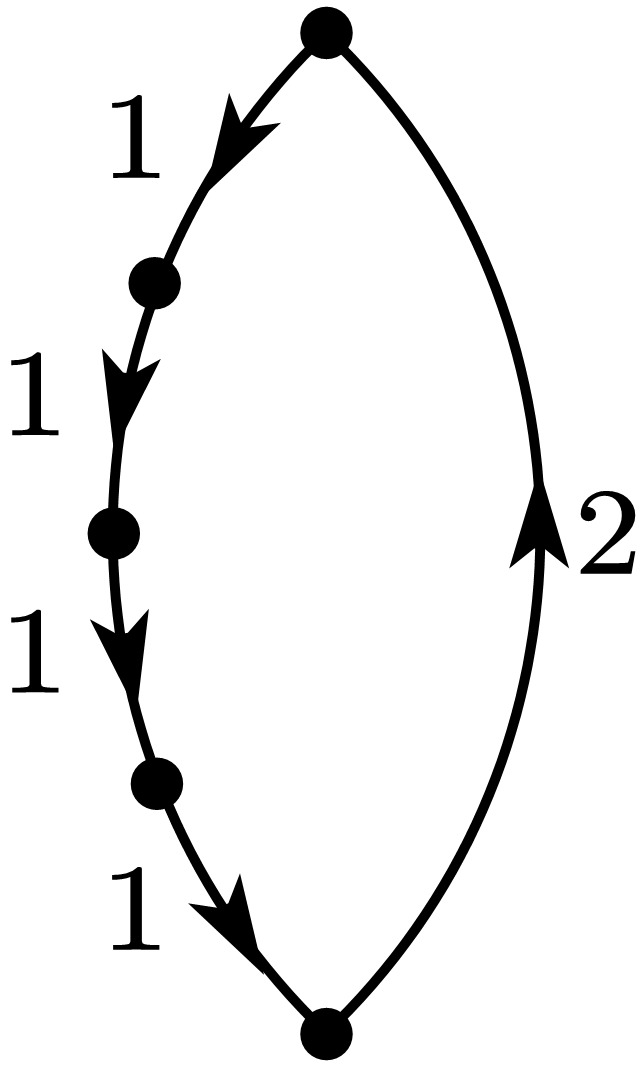
\includegraphics[scale=1.0,trim=0 -4 0 -4]{./pictures/6.01/1.png}
		\captionof*{figure}{$\displaystyle (-1)^{4+1} \frac{ V^3_{11} V_{12} V_{21} }{ ( E^{(0)}_1 - E^{(0)}_2)^4 }$}
		\end{minipage} &
		
		\begin{minipage}{0.22\linewidth}
		\centering
		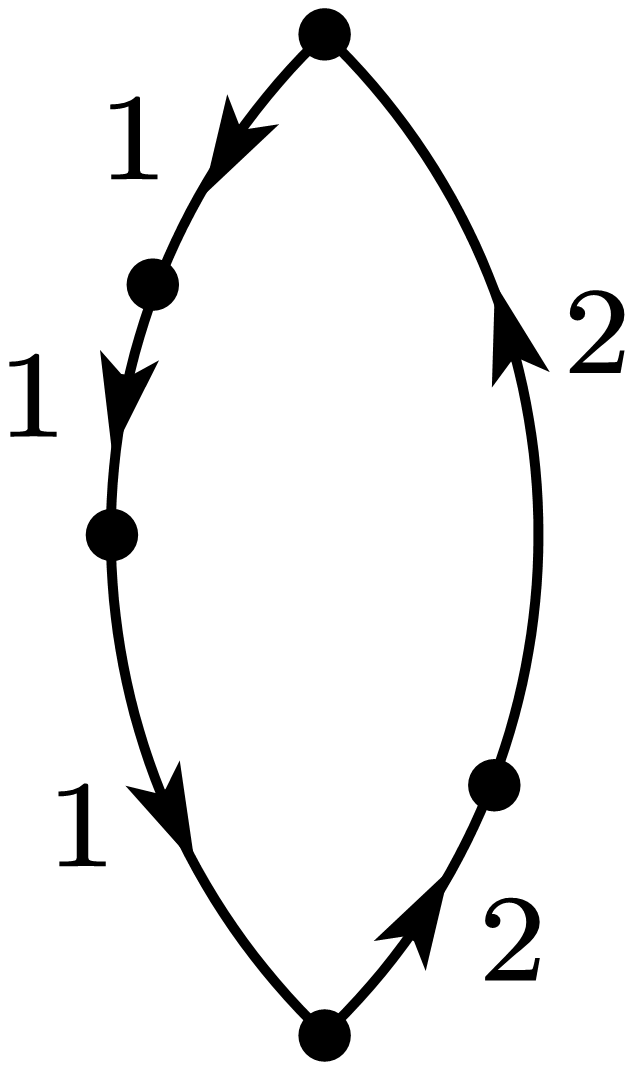
\includegraphics[scale=1.0,trim=0 -4 0 -4]{./pictures/6.01/2.png}
		\captionof*{figure}{$\displaystyle (-1)^{3+1} \frac{ V^2_{11} V_{12} V_{21} V_{22} }{ ( E^{(0)}_1 - E^{(0)}_2)^4 }$}
		\end{minipage} &
		
		\begin{minipage}{0.22\linewidth}
		\centering
		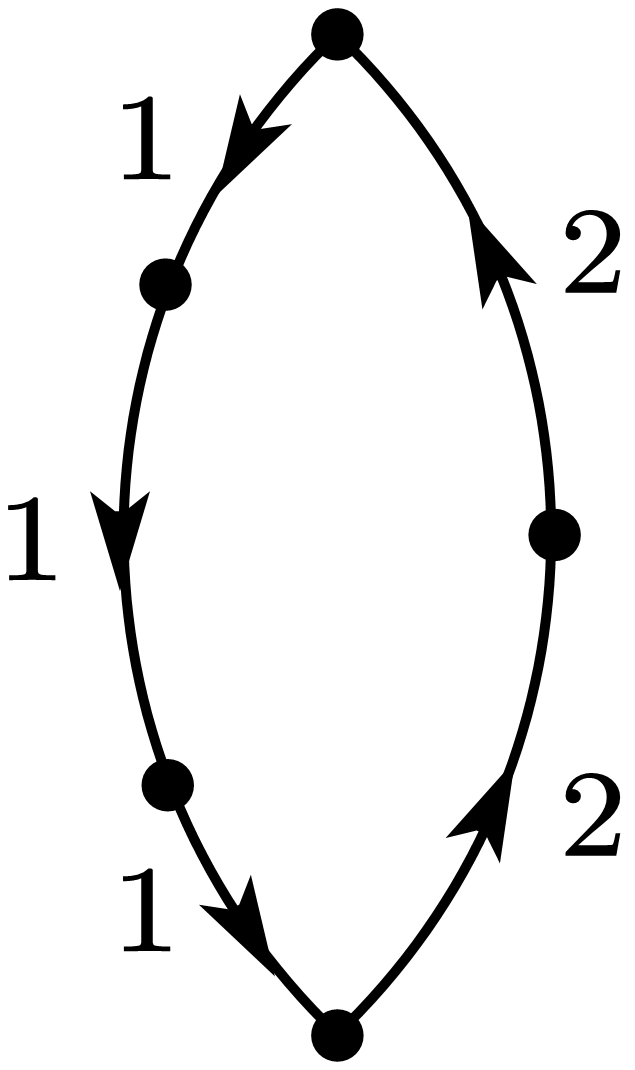
\includegraphics[scale=1.0,trim=0 -4 0 -4]{./pictures/6.01/3.png}
		\captionof*{figure}{$\displaystyle (-1)^{3+1} \frac{ V^2_{11} V_{12} V_{21} V_{22} }{ ( E^{(0)}_1 - E^{(0)}_2)^4 }$}
		\end{minipage} &
		
		\begin{minipage}{0.22\linewidth}
		\centering
		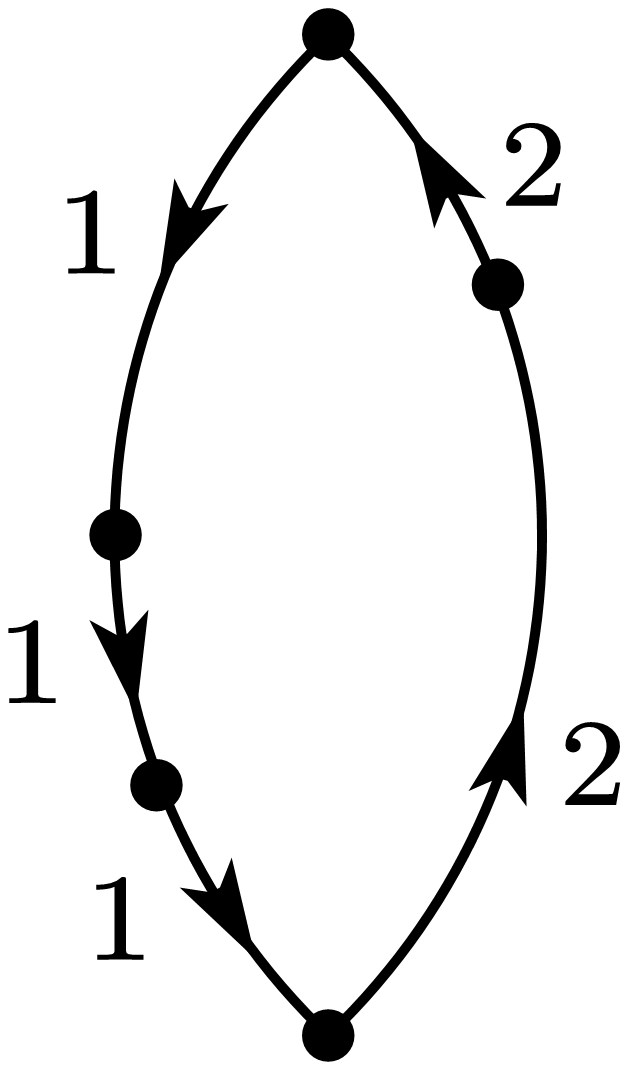
\includegraphics[scale=1.0,trim=0 -4 0 -4]{./pictures/6.01/4.png}
		\captionof*{figure}{$\displaystyle (-1)^{3+1} \frac{ V^2_{11} V_{12} V_{21} V_{22} }{ ( E^{(0)}_1 - E^{(0)}_2)^4 }$}
		\end{minipage} \\
			
		\begin{minipage}{0.22\linewidth}
		\centering
		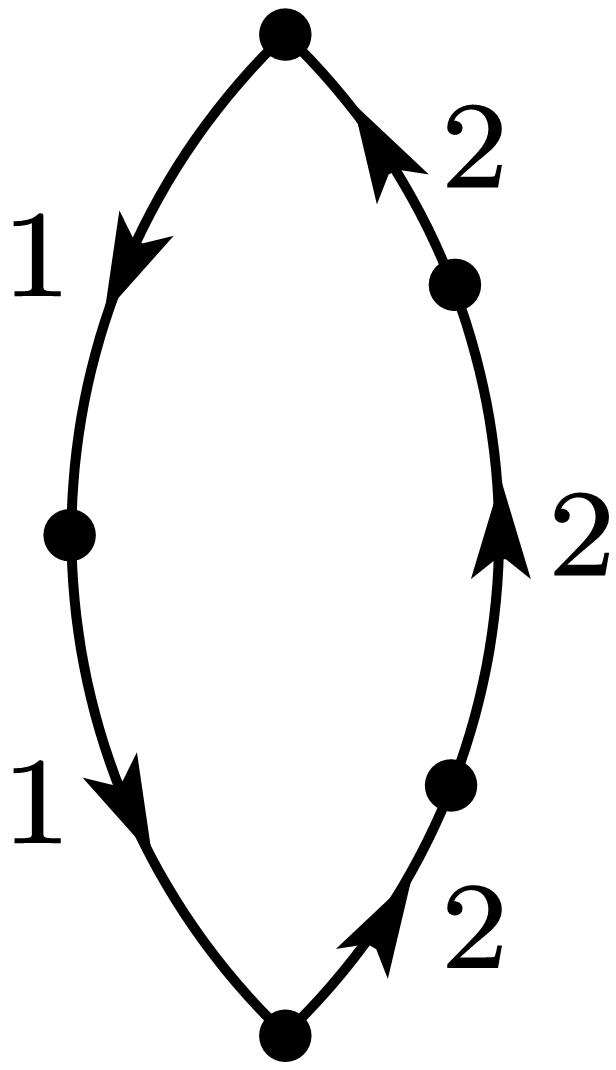
\includegraphics[scale=1.0,trim=0 -4 0 -4]{./pictures/6.01/5.png}
		\captionof*{figure}{$\displaystyle (-1)^{2+1} \frac{ V_{11} V_{12} V_{21} V^2_{22} }{ ( E^{(0)}_1 - E^{(0)}_2)^4 }$}
		\end{minipage} &
		
		\begin{minipage}{0.22\linewidth}
		\centering
		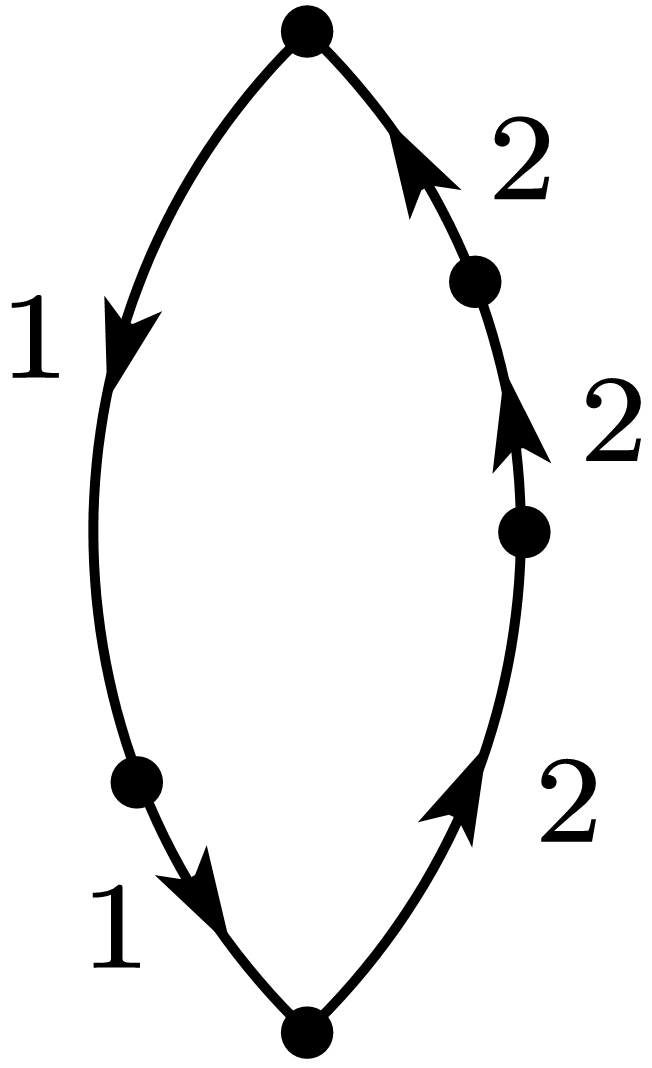
\includegraphics[scale=1.0,trim=0 -4 0 -4]{./pictures/6.01/6.png}
		\captionof*{figure}{$\displaystyle (-1)^{2+1} \frac{ V_{11} V_{12} V_{21} V^2_{22} }{ ( E^{(0)}_1 - E^{(0)}_2)^4 }$}
		\end{minipage} &
		
		\begin{minipage}{0.22\linewidth}
		\centering
		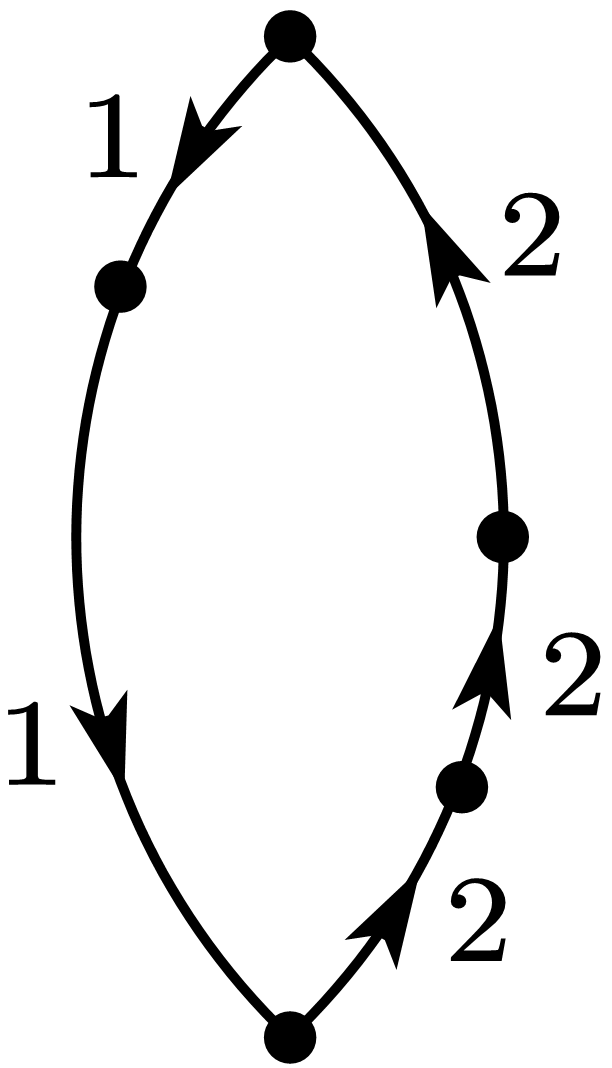
\includegraphics[scale=1.0,trim=0 -4 0 -4]{./pictures/6.01/7.png}
		\captionof*{figure}{$\displaystyle (-1)^{2+1} \frac{ V_{11} V_{12} V_{21} V^2_{22} }{ ( E^{(0)}_1 - E^{(0)}_2)^4 }$}
		\end{minipage} &
		
		\begin{minipage}{0.22\linewidth}
		\centering
		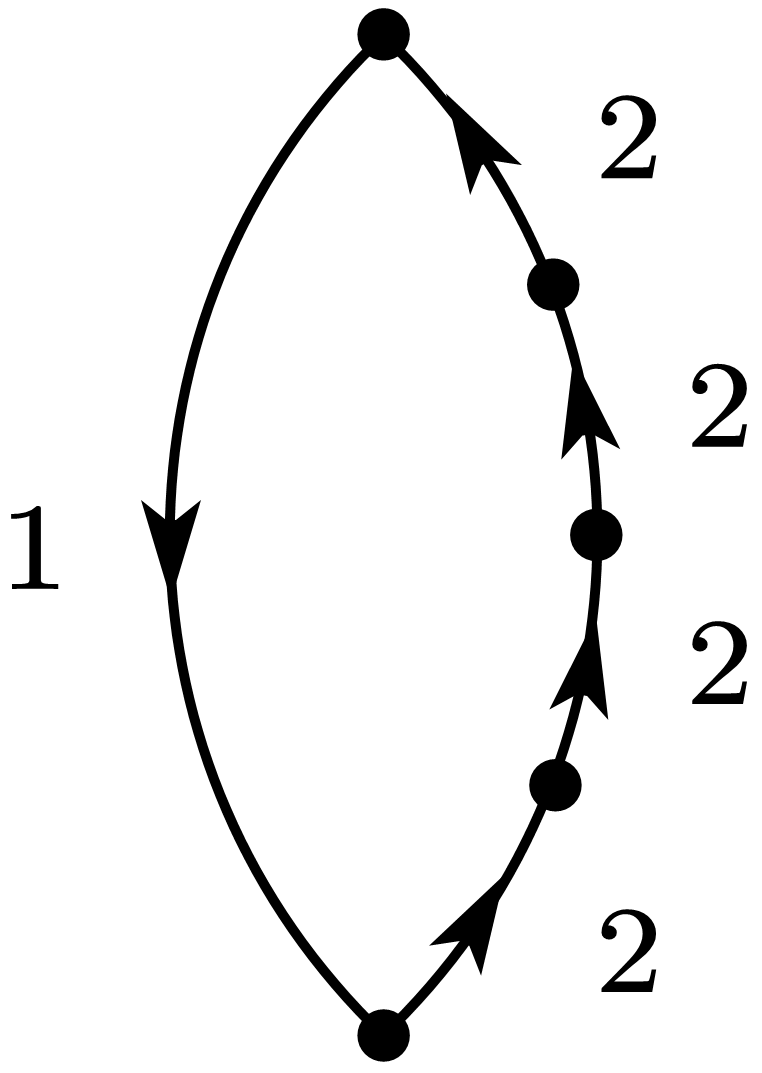
\includegraphics[scale=1.0,trim=0 -4 0 -4]{./pictures/6.01/8.png}
		\captionof*{figure}{$\displaystyle (-1)^{1+1} \frac{ V_{12} V_{21} V^3_{22} }{ ( E^{(0)}_1 - E^{(0)}_2)^4 }$}
		\end{minipage} 
		
	\end{tabular}
	\captionof{figure}{All fifth-order diagrams, which have the property that an imaginary horizontal line crosses only one hole and one particle line, and their mathematical expressions.}\label{fig:exe1}
	\end{center}
	
	Note that the diagrams, which have the property that an imaginary horizontal line crosses only one hole and one particle line, have no pair of hole/particle lines whose overlap is nonempty. For any pair of hole/particle lines which connect the dots $m_1$ and $n_1$, $m_2$ and $n_2$, where $n_1 > m_1$ and $n_2 > m_2$, their overlap will be 
	\begin{itemize}
	
	\item $[\max\{m_1, m_2\},\min\{n_1, n_2\}]$, if $\min\{n_1, n_2\} > \max\{m_1, m_2\}$;
	
	\item empty, otherwise. 
	
	\end{itemize}
	For example, if there is a pair of hole lines, one connecting the dot 1 and 3, and the other connecting 2 and 5, their overlap will be $[2, 3]$. Take an another example, if there is a pair of particle lines, one connecting the dot 5 and 4, and the other connecting 2 and 1, their overlap will be empty.
	
	Thus, there are four cases.
	\begin{itemize}
	
	\item Four hole lines and one particle line. There is only one method, hole lines are $(1,2)$, $(2,3)$, $(3,4)$, $(4,5)$ and the only particle line is $(5,1)$, as the first subdiagram in \Figref{fig:exe1}.
	
	\item Three hole lines and two particle lines. There are three methods as follows.
		\begin{itemize}
	
		\item Hole lines are $(1,2)$, $(2,3)$, and $(3,5)$ while particle lines are $(5,4)$, $(4,1)$.
		
		\item Hole lines are $(1,2)$, $(2,4)$, and $(4,5)$ while particle lines are $(5,3)$, $(3,1)$.
		
		\item Hole lines are $(1,3)$, $(3,4)$, and $(4,5)$ while particle lines are $(5,2)$, $(2,1)$.
	
		\end{itemize}
		They correspond to the second, third, fourth subdiagram in \Figref{fig:exe1}.
	
	\item Two hole lines and three particle lines. There are three methods as follows.
		\begin{itemize}
	
		\item Hole lines are $(1,3)$, $(3,5)$ while particle lines are $(5,4)$, $(4,2)$, and $(2,1)$.
		
		\item Hole lines are $(1,4)$, $(4,5)$ while particle lines are $(5,3)$, $(3,2)$, and $(2,1)$.
		
		\item Hole lines are $(1,2)$, $(2,5)$ while particle lines are $(5,4)$, $(4,3)$, and $(3,1)$.
	
		\end{itemize}
		They correspond to the fifth, sixth, seventh subdiagram in \Figref{fig:exe1}.
		
	\item One hole line and four particle lines. There is only one method, the only hole line is $(1,5)$ and particle lines are $(5,4)$, $(4,3)$, $(3,2)$, and $(2,1)$, as the eighth subdiagram in \Figref{fig:exe1}.
			
	\end{itemize}
	
	Thus, the sum of such diagrams is
	\begin{align*}
%		&\hspace{1.4em}(-1)^{4+1} \frac{ V^3_{11} V_{12} V_{21} }{ ( E^{(0)}_1 - E^{(0)}_2)^4 } + (-1)^{3+1} \frac{ V^2_{11} V_{12} V_{21} V_{22} }{ ( E^{(0)}_1 - E^{(0)}_2)^4 } + (-1)^{3+1} \frac{ V^2_{11} V_{12} V_{21} V_{22} }{ ( E^{(0)}_1 - E^{(0)}_2)^4 } \\
%		&\hspace{1.4em} + (-1)^{3+1} \frac{ V^2_{11} V_{12} V_{21} V_{22} }{ ( E^{(0)}_1 - E^{(0)}_2)^4 } + (-1)^{2+1} \frac{ V_{11} V_{12} V_{21} V^2_{22} }{ ( E^{(0)}_1 - E^{(0)}_2) }^4 + (-1)^{2+1} \frac{ V_{11} V_{12} V_{21} V^2_{22} }{ ( E^{(0)}_1 - E^{(0)}_2) }^4 \\
%		&\hspace{1.4em}  + (-1)^{2+1} \frac{ V_{11} V_{12} V_{21} V^2_{22} }{ ( E^{(0)}_1 - E^{(0)}_2) }^4 + (-1)^{1+1} \frac{ V_{12} V_{21} V^3_{22} }{ ( E^{(0)}_1 - E^{(0)}_2)^4 } \\
%		&= - \frac{ V^3_{11} V_{12} V_{21} }{ ( E^{(0)}_1 - E^{(0)}_2)^4 } + 3 \frac{ V^2_{11} V_{12} V_{21} V_{22} }{ ( E^{(0)}_1 - E^{(0)}_2)^4 } - 3 \frac{ V_{11} V_{12} V_{21} V^2_{22} }{ ( E^{(0)}_1 - E^{(0)}_2) }^4 + \frac{ V_{12} V_{21} V^3_{22} }{ ( E^{(0)}_1 - E^{(0)}_2)^4 } \\
%		&= 
		- \frac{ V_{12} V_{21} \left( V^3_{11} - 3 V^2_{11} V_{22} + 3 V_{11} V_{22} - V^3_{22} \right) }{ ( E^{(0)}_1 - E^{(0)}_2)^4 } = - \frac{ V_{12} V_{21} \left( V_{11} - V_{22} \right)^3 }{ ( E^{(0)}_1 - E^{(0)}_2)^4 } = \frac{ V_{12} V_{21} \left( V_{22} - V_{11} \right)^3 }{ ( E^{(0)}_1 - E^{(0)}_2)^4 }.
	\end{align*}
	
	In fact, as the textbook says, these eight diagrams can be generated by adding three dots to the second-order diagram in all positive ways. In fact, any pair of hole/particle lines in them has also empty overlap. I think the calculation of the overlap is much direct than inspecting the property of lines.
	
	\end{solution}

	\subsection{Diagrammatic Perturbation Theory for \texorpdfstring{$N$}- States}
	
	% 6.2
	\begin{exercise}
	Use diagrammatic techniques to obtain the fourth-order perturbation energy of a particular state (say, $i$) of an $N$-state system. That is, evaluate the diagrams
	\begin{center}
	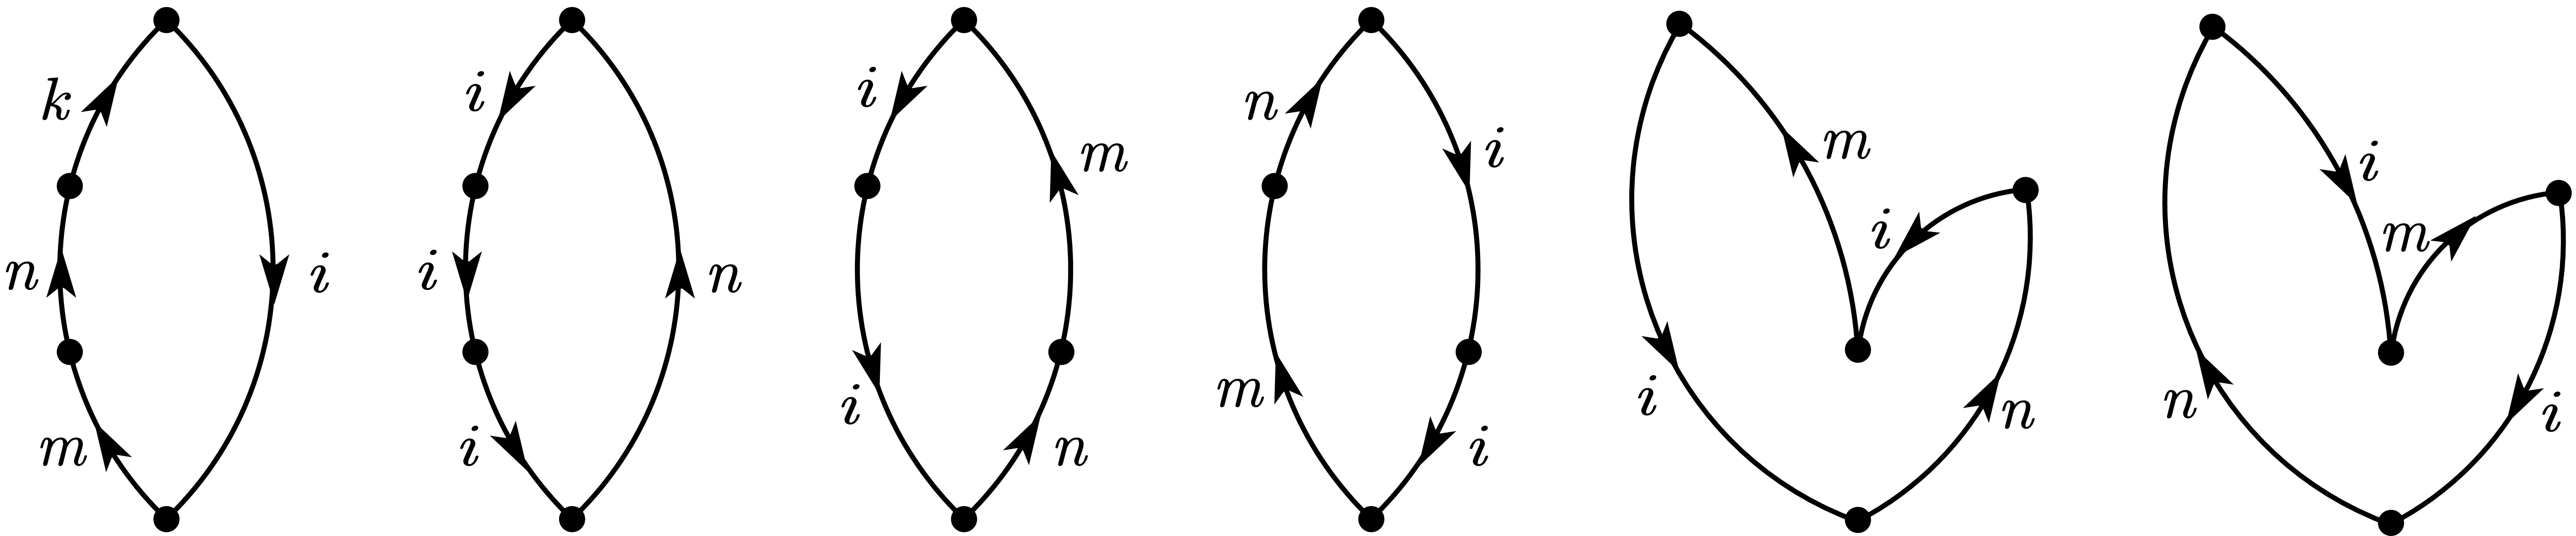
\includegraphics[scale=1.0]{./pictures/6.02/exercise.png}
	\end{center}
	where the indices $m$, $n$, $k$, ... exclude $i$. Using the approach of Section 6.1, obtain an algebraic expression for the fourth-order energy and compare it to the diagrammatic result.
	
	\end{exercise}
	
	\begin{solution}
	
	Firstly, all fourth-order diagrams and their mathematical expressions are listed in \Figref{fig:exe2}.
	
	\begin{center}
	\begin{tabular}{cc}
	
		\begin{minipage}{0.49\linewidth}
		\centering
		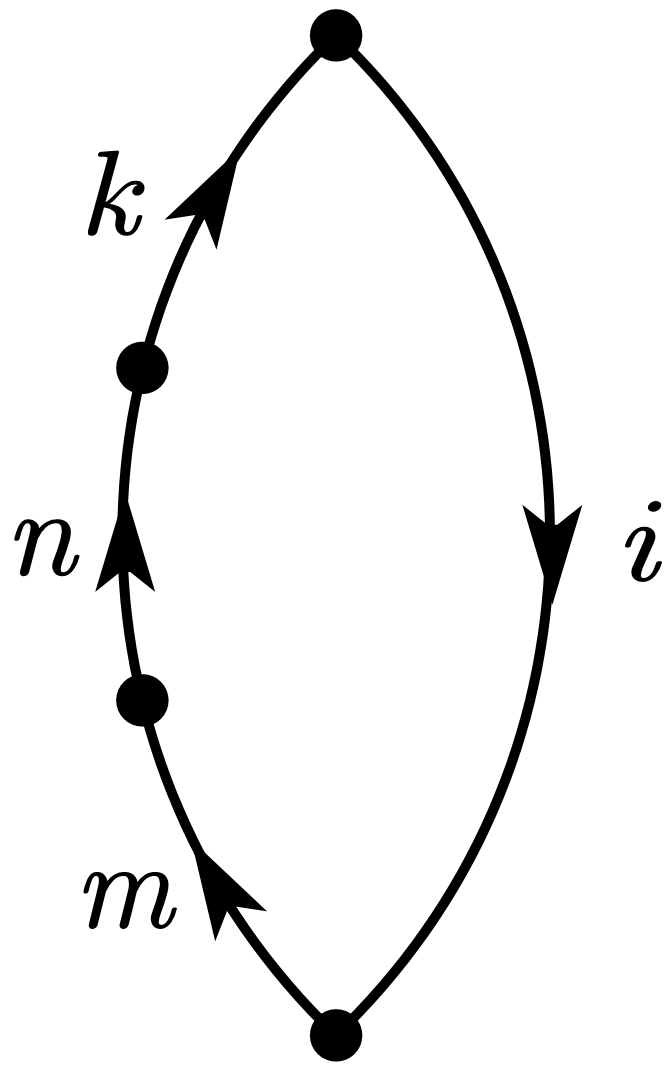
\includegraphics[scale=1.0,trim=0 -4 0 -4]{./pictures/6.02/1.png}
		\captionof*{figure}{$(-1)^{1+1} { \sum_{kmn} }^\prime \frac{ V_{ki} V_{nk} V_{mn} V_{im} }{ ( E^{(0)}_i - E^{(0)}_k ) ( E^{(0)}_i - E^{(0)}_n ) ( E^{(0)}_i - E^{(0)}_m ) }$}
		\end{minipage} &
		
		\begin{minipage}{0.42\linewidth}
		\centering
		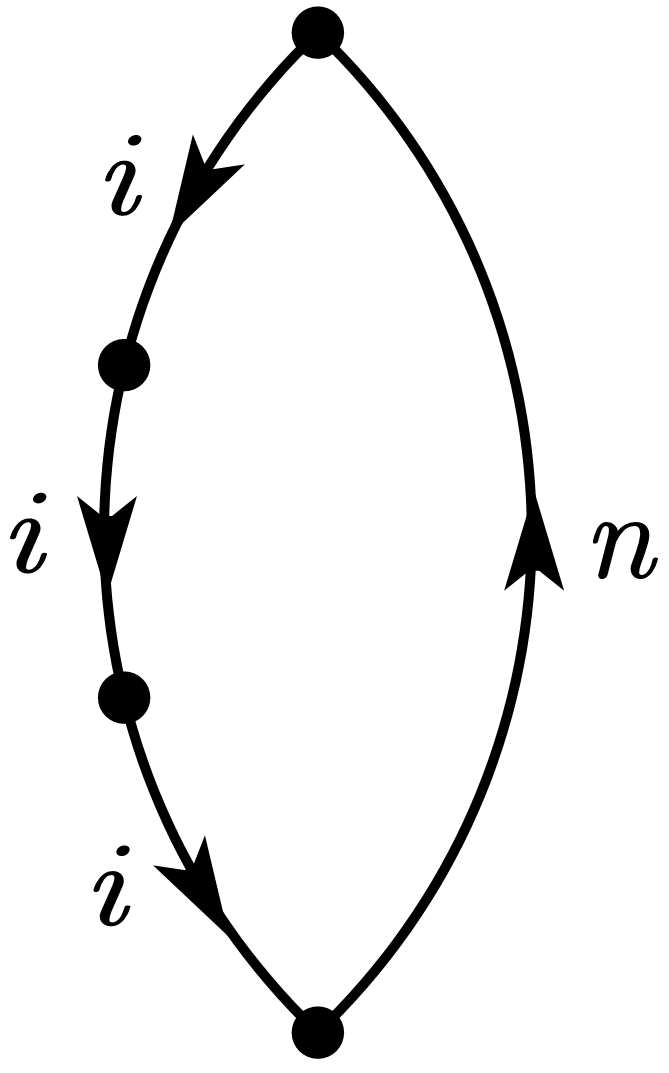
\includegraphics[scale=1.0,trim=0 -4 0 -4]{./pictures/6.02/2.png}
		\captionof*{figure}{$(-1)^{3+1} { \sum_n }^\prime \frac{ V_{ni} V^2_{ii} V_{in} }{ ( E^{(0)}_i - E^{(0)}_n)^3 }$}
		\end{minipage} \\
		
		\begin{minipage}{0.49\linewidth}
		\centering
		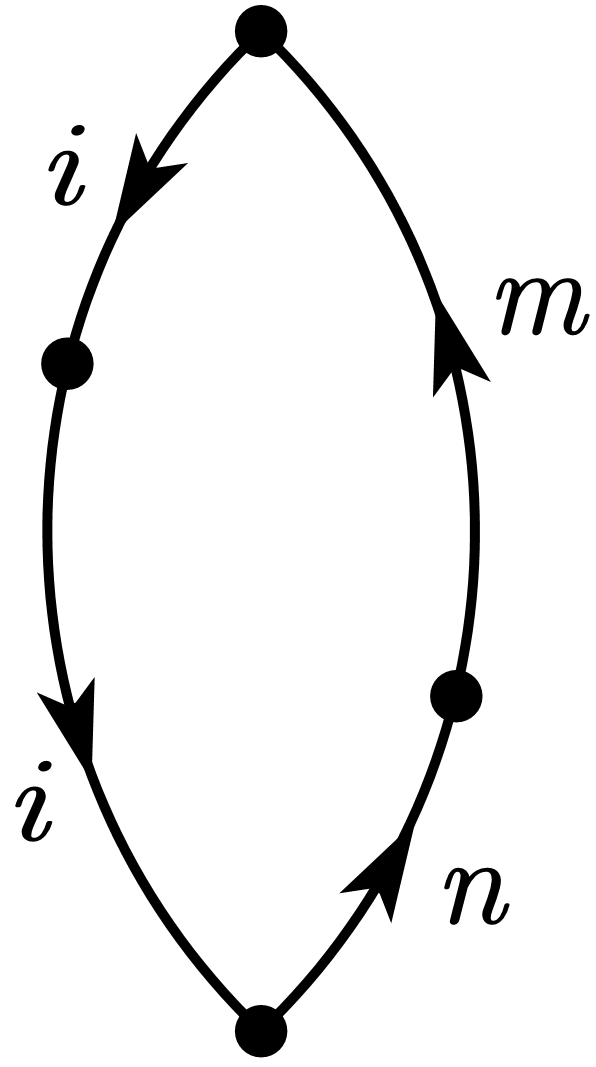
\includegraphics[scale=1.0,trim=0 -4 0 -4]{./pictures/6.02/3.png}
		\captionof*{figure}{$(-1)^{2+1} { \sum_{mn} }^\prime \frac{ V_{mi} V_{ii} V_{in} V_{nm} }{ ( E^{(0)}_i - E^{(0)}_n) ( E^{(0)}_i - E^{(0)}_m )^2 }$}
		\end{minipage}  &
			
		\begin{minipage}{0.42\linewidth}
		\centering
		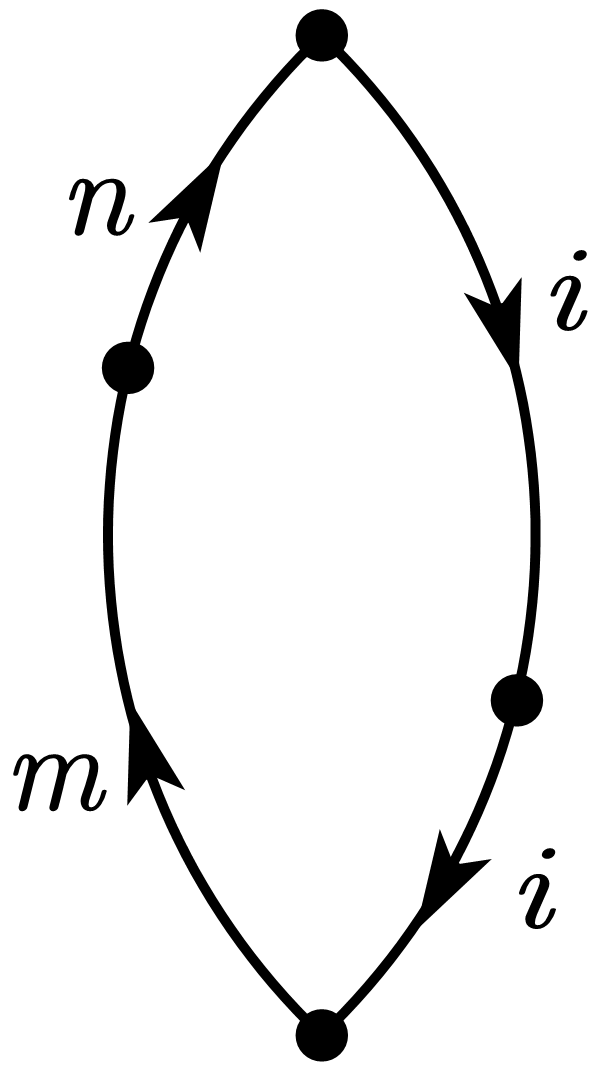
\includegraphics[scale=1.0,trim=0 -4 0 -4]{./pictures/6.02/4.png}
		\captionof*{figure}{$(-1)^{2+1} { \sum_{mn} }^\prime \frac{ V_{ni} V_{ii} V_{im} V_{mn} }{ ( E^{(0)}_i - E^{(0)}_n) ( E^{(0)}_i - E^{(0)}_m )^2 }$}
		\end{minipage} \\
		
		\begin{minipage}{0.49\linewidth}
		\centering
		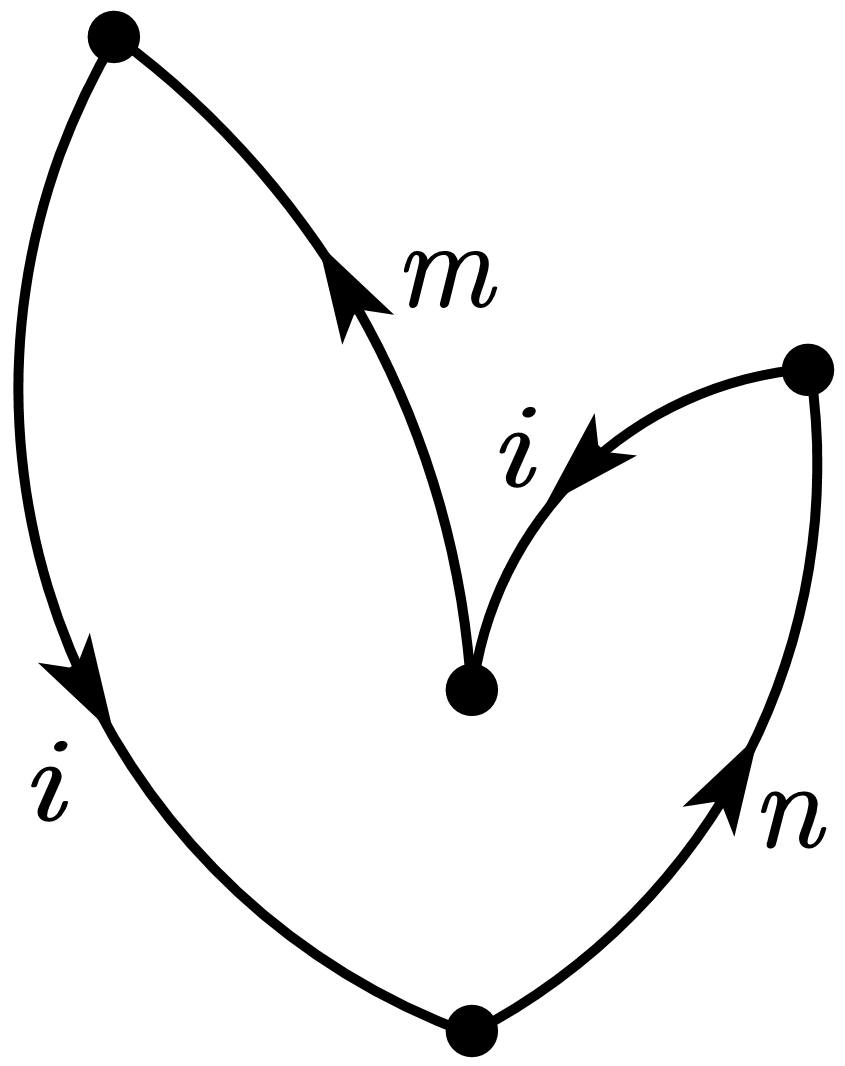
\includegraphics[scale=1.0,trim=0 -4 0 -4]{./pictures/6.02/5.png}
		\captionof*{figure}{$(-1)^{2+1} { \sum_{mn} }^\prime \frac{ V_{mi} V_{in} V_{ni} V_{im} }{ ( E^{(0)}_i - E^{(0)}_m ) ( 2E^{(0)}_i - E^{(0)}_m - E^{(0)}_n ) ( E^{(0)}_i - E^{(0)}_n ) }$}
		\end{minipage} &
		
		\begin{minipage}{0.42\linewidth}
		\centering
		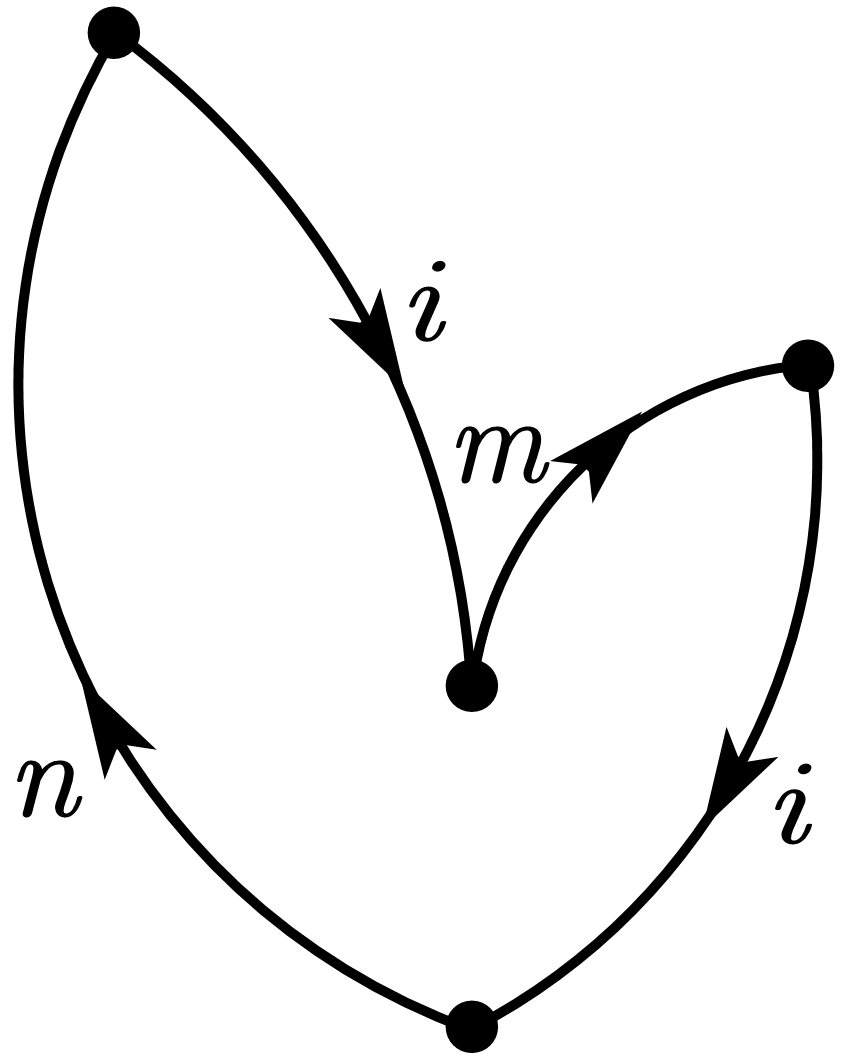
\includegraphics[scale=1.0,trim=0 -4 0 -4]{./pictures/6.02/6.png}
		\captionof*{figure}{$(-1)^{2+1} { \sum_{mn} }^\prime \frac{ V_{in} V_{ni} V_{im} V_{mi} }{ ( 2E^{(0)}_i - E^{(0)}_m - E^{(0)}_n ) ( E^{(0)}_i - E^{(0)}_n )^2 }$}
		\end{minipage} 
				
	\end{tabular}
	\captionof{figure}{All fourth-order diagrams and their mathematical expressions.}\label{fig:exe2}
	\end{center}
	
	Before the formal algebraic derivation, we should obtain some useful intermediate results. From (6.7d), multiplying by $\langle n |$, where $n \neq i$, we find that
	\[
		E^{(0)}_n \langle n | \Psi^{(3)}_i \rangle + \langle n | \mathscr{V} | \Psi^{(2)}_i \rangle = E^{(0)}_i \langle n | \Psi^{(3)}_i \rangle + E^{(1)}_i \langle n | \Psi^{(2)}_i \rangle + E^{(1)}_i \langle n | \Psi^{(2)}_i \rangle,
	\]
	and thus
	\[
		\langle n | \Psi^{(3)}_i \rangle = \frac{ 1 }{ E^{(0)}_i - E^{(0)}_n }\left[ \langle n | \mathscr{V} | \Psi^{(2)}_i \rangle - E^{(1)}_i \langle n | \Psi^{(2)}_i \rangle - E^{(1)}_i \langle n | \Psi^{(2)}_i \rangle \right].
	\]
	Moreover, (6.8b), (6.10), (6.12), and (6.14) are used in the formal derivation. The fourth-order perturbation energy $E^{(4)}_i$ can be divided into 3 terms, viz.,
	\begin{align*}
		E^{(4)}_i &= \langle i | \mathscr{V} | \Psi^{(3)}_i \rangle = { \sum_n }^\prime \langle i | \mathscr{V} | n \rangle \langle n | \Psi^{(3)}_i \rangle = { \sum_n }^\prime V_{in} \frac{ \langle n | \mathscr{V} | \Psi^{(2)}_i \rangle - E^{(1)}_i \langle n | \Psi^{(2)}_i \rangle - E^{(2)}_i \langle n | \Psi^{(1)}_i \rangle }{ E^{(0)}_i - E^{(0)}_n } \\
		&= { \sum_n }^\prime \frac{ V_{in} \langle n | \mathscr{V} | \Psi^{(2)}_i \rangle }{ E^{(0)}_i - E^{(0)}_n } - E^{(1)}_i { \sum_n }^\prime \frac{ V_{in} \langle n | \Psi^{(2)}_i \rangle }{ E^{(0)}_i - E^{(0)}_n } - E^{(2)}_i { \sum_n }^\prime \frac{ V_{in} \langle n | \Psi^{(1)}_i \rangle }{ E^{(0)}_i - E^{(0)}_n }.
	\end{align*}		
	The first term is
	\begin{align*}
		&\hspace{1.4em}{ \sum_n }^\prime \frac{ V_{in} \langle n | \mathscr{V} | \Psi^{(2)}_i \rangle }{ E^{(0)}_i - E^{(0)}_n } = { \sum_{mn} }^\prime \frac{ V_{in} \langle n | \mathscr{V} | m \rangle \langle m | \Psi^{(2)}_i \rangle }{ E^{(0)}_i - E^{(0)}_n } = { \sum_{mn} }^\prime \frac{ V_{in} V_{nm} }{ E^{(0)}_i - E^{(0)}_n } \langle m | \Psi^{(2)}_i \rangle \\
		&= { \sum_{mn} }^\prime \frac{ V_{in} V_{nm} }{ E^{(0)}_i - E^{(0)}_n } \frac{ \langle m | \mathscr{V} | \Psi^{(1)}_i \rangle - E^{(1)}_i \langle m | \Psi^{(1)}_i \rangle }{ E^{(0)}_i - E^{(0)}_m } \\
		&= { \sum_{mn} }^\prime \frac{ V_{in} V_{nm} }{ ( E^{(0)}_i - E^{(0)}_n )( E^{(0)}_i - E^{(0)}_m ) } \left[ \langle m | \mathscr{V} | \Psi^{(1)}_i \rangle - E^{(1)}_i \langle m | \Psi^{(1)}_i \rangle \right] \\
		&= { \sum_{mn} }^\prime \frac{ V_{in} V_{nm} }{ (E^{(0)}_i - E^{(0)}_n) (E^{(0)}_i - E^{(0)}_m) } \left[ { \sum_k }^\prime \langle m | \mathscr{V} | k \rangle \langle k | \Psi^{(1)}_i \rangle - E^{(1)}_i \langle m | \Psi^{(1)}_i \rangle \right] \\
		&= { \sum_{mnk} }^\prime \frac{ V_{in} V_{nm} V_{mk} }{ (E^{(0)}_i - E^{(0)}_n) (E^{(0)}_i - E^{(0)}_m) } \langle k | \Psi^{(1)}_i \rangle - { \sum_{mn} }^\prime \frac{ V_{ii} V_{in} V_{nm} }{ (E^{(0)}_i - E^{(0)}_n) (E^{(0)}_i - E^{(0)}_m) } \langle m | \Psi^{(1)}_i \rangle \\
		&= { \sum_{mnk} }^\prime \frac{ V_{in} V_{nm} V_{mk} }{ (E^{(0)}_i - E^{(0)}_n) (E^{(0)}_i - E^{(0)}_m) } \frac{ V_{ki} }{ E^{(0)}_i - E^{(0)}_k } - { \sum_{mn} }^\prime \frac{ V_{ii} V_{in} V_{nm} }{ (E^{(0)}_i - E^{(0)}_n) (E^{(0)}_i - E^{(0)}_m) } \frac{ V_{mi} }{ E^{(0)}_i - E^{(0)}_m } \\
		&= { \sum_{mnk} }^\prime \frac{ V_{in} V_{nm} V_{mk} V_{ki} }{ (E^{(0)}_i - E^{(0)}_n) (E^{(0)}_i - E^{(0)}_m) (E^{(0)}_i - E^{(0)}_k) } - { \sum_{mn} }^\prime \frac{ V_{ii} V_{in} V_{nm} V_{mi} }{ (E^{(0)}_i - E^{(0)}_n) (E^{(0)}_i - E^{(0)}_m)^2 } \\
		&= { \sum_{mnk} }^\prime \frac{ V_{im} V_{mn} V_{nk} V_{ki} }{ (E^{(0)}_i - E^{(0)}_n) (E^{(0)}_i - E^{(0)}_m) (E^{(0)}_i - E^{(0)}_k) } - { \sum_{mn} }^\prime \frac{ V_{ii} V_{in} V_{nm} V_{mi} }{ (E^{(0)}_i - E^{(0)}_n) (E^{(0)}_i - E^{(0)}_m)^2 }.
	\end{align*}
	It is evident that the first part of the first term correspond to the first subdiagram and the second part of the first term correspond to the third subdiagram.
	
	The second term is
	\begin{align*}
		&\hspace{1.4em}- E^{(1)}_i { \sum_n }^\prime \frac{ V_{in} \langle n | \Psi^{(2)}_i \rangle }{ E^{(0)}_i - E^{(0)}_n } - { \sum_n }^\prime \frac{ V_{ii} V_{in} }{ E^{(0)}_i - E^{(0)}_n } \langle n | \Psi^{(2)}_i \rangle \\
		&= - { \sum_n }^\prime \frac{ V_{ii} V_{in} }{ E^{(0)}_i - E^{(0)}_n } \frac{ \langle n | \mathscr{V} | \Psi^{(1)}_i \rangle - E^{(1)}_i \langle n | \Psi^{(1)}_i \rangle }{ E^{(0)}_i - E^{(0)}_n } \\
		&= - { \sum_n }^\prime \frac{ V_{ii} V_{in} }{ ( E^{(0)}_i - E^{(0)}_n )^2 } \langle n | \mathscr{V} | \Psi^{(1)}_i \rangle + E^{(1)}_i { \sum_n }^\prime \frac{ V_{ii} V_{in} }{ ( E^{(0)}_i - E^{(0)}_n )^2 } \langle n | \Psi^{(1)}_i \rangle \\
		&= - { \sum_n }^\prime \frac{ V_{ii} V_{in} }{ ( E^{(0)}_i - E^{(0)}_n )^2 } { \sum_m }^\prime \langle n | \mathscr{V} | m \rangle \langle m | \Psi^{(1)}_i \rangle + { \sum_n }^\prime \frac{ V^2_{ii} V_{in} }{ ( E^{(0)}_i - E^{(0)}_n )^2 } \langle n | \Psi^{(1)}_i \rangle \\
		&= - { \sum_{mn} }^\prime \frac{ V_{ii} V_{in} V_{nm} }{ ( E^{(0)}_i - E^{(0)}_n )^2 } \langle m | \Psi^{(1)}_i \rangle + { \sum_n }^\prime \frac{ V^2_{ii} V_{in} }{ ( E^{(0)}_i - E^{(0)}_n )^2 } \langle n | \Psi^{(1)}_i \rangle \\
		&= - { \sum_{mn} }^\prime \frac{ V_{ii} V_{in} V_{nm} }{ ( E^{(0)}_i - E^{(0)}_n )^2 } \frac{ \langle m | \mathscr{V} | i \rangle }{ E^{(0)}_i - E^{(0)}_m } + { \sum_n }^\prime \frac{ V^2_{ii} V_{in} }{ ( E^{(0)}_i - E^{(0)}_n )^2 } \frac{ \langle n | \mathscr{V} | i \rangle }{ E^{(0)}_i - E^{(0)}_n } \\
		&= - { \sum_{mn} }^\prime \frac{ V_{ii} V_{in} V_{nm} V_{mi} }{ ( E^{(0)}_i - E^{(0)}_n )^2 (E^{(0)}_i - E^{(0)}_m) } + { \sum_n }^\prime \frac{ V^2_{ii} V_{in} V_{ni} }{ ( E^{(0)}_i - E^{(0)}_n )^3 } \\
		&= - { \sum_{mn} }^\prime \frac{ V_{ii} V_{im} V_{mn} V_{ni} }{ ( E^{(0)}_i - E^{(0)}_m )^2 ( E^{(0)}_i - E^{(0)}_n ) } + { \sum_n }^\prime \frac{ V^2_{ii} V_{in} V_{ni} }{ ( E^{(0)}_i - E^{(0)}_n )^3 } .
	\end{align*}
	It is evident that the first part of the second term correspond to the fourth subdiagram and the second part of the second term correspond to the second subdiagram.
	
	The third term is
	\begin{align*}
		&\hspace{1.4em} -E^{(2)}_i { \sum_n }^\prime \frac{ V_{in} \langle n | \Psi^{(1)}_i \rangle }{ E^{(0)}_i - E^{(0)}_n } = -E^{(2)}_i { \sum_n }^\prime \frac{ V_{in} }{ E^{(0)}_i - E^{(0)}_n } \frac{ \langle n | \mathscr{V} | i \rangle }{ E^{(0)}_i - E^{(0)}_n } = -E^{(2)}_i { \sum_n }^\prime \frac{ V_{in} V_{ni} }{ ( E^{(0)}_i - E^{(0)}_n )^2 } \\
		&= - \left( { \sum_m }^\prime \frac{ V_{im} V_{mi} }{ ( E^{(0)}_i - E^{(0)}_m ) } \right) { \sum_n }^\prime \frac{ V_{in} V_{ni} }{ ( E^{(0)}_i - E^{(0)}_n )^2 } = - { \sum_{mn} }^\prime \frac{ V_{im} V_{mi} V_{in} V_{ni} }{ ( E^{(0)}_i - E^{(0)}_m )( E^{(0)}_i - E^{(0)}_n )^2 } .
	\end{align*}		
	
	It seems that it does not directly correspond to any subdiagram in \Figref{fig:exe2}. However, we can find that the sum of the mathematical expressions of the fifth and sixth subdiagram is
	\begin{align*}
		&\hspace{1.4em}(-1)^{2+1} { \sum_{mn} }^\prime \frac{ V_{mi} V_{in} V_{ni} V_{im} }{ ( E^{(0)}_i - E^{(0)}_m ) ( 2E^{(0)}_i - E^{(0)}_m - E^{(0)}_n ) ( E^{(0)}_i - E^{(0)}_n ) }  \\
		&\hspace{3.4em}+ (-1)^{2+1} { \sum_{mn} }^\prime \frac{ V_{in} V_{ni} V_{im} V_{mi} }{ ( 2E^{(0)}_i - E^{(0)}_m - E^{(0)}_n ) ( E^{(0)}_i - E^{(0)}_n )^2 } \\
		&= - { \sum_{mn} }^\prime \frac{ V_{in} V_{ni} V_{im} V_{mi} }{ ( 2E^{(0)}_i - E^{(0)}_m - E^{(0)}_n ) ( E^{(0)}_i - E^{(0)}_n ) } \left[ \frac{ 1 }{ E^{(0)}_i - E^{(0)}_m } + \frac{ 1 }{ E^{(0)}_i - E^{(0)}_n } \right] \\
		&= - { \sum_{mn} }^\prime \frac{ V_{in} V_{ni} V_{im} V_{mi} }{ ( 2E^{(0)}_i - E^{(0)}_m - E^{(0)}_n ) ( E^{(0)}_i - E^{(0)}_n ) } \frac{ 2E^{(0)}_i - E^{(0)}_m - E^{(0)}_n }{ ( E^{(0)}_i - E^{(0)}_m )( E^{(0)}_i - E^{(0)}_n ) } \\
		&= - { \sum_{mn} }^\prime \frac{ V_{im} V_{mi} V_{in} V_{ni} }{ ( E^{(0)}_i - E^{(0)}_m )( E^{(0)}_i - E^{(0)}_n )^2 } ,
	\end{align*}
	which is the third term exactly. Thus we can conclude that the results obtained by algebraic methods is the same as that by diagrammatic techniques. The mathematical expression of the fourth-order perturbation energy $E^{(4)}_i$ is
	\begin{align*}
		E^{(4)}_i &= { \sum_{mnk} }^\prime \frac{ V_{im} V_{mn} V_{nk} V_{ki} }{ (E^{(0)}_i - E^{(0)}_n) (E^{(0)}_i - E^{(0)}_m) (E^{(0)}_i - E^{(0)}_k) } - { \sum_{mn} }^\prime \frac{ V_{ii} V_{in} V_{nm} V_{mi} }{ (E^{(0)}_i - E^{(0)}_n) (E^{(0)}_i - E^{(0)}_m)^2 } \\
		&\hspace{2em} - { \sum_{mn} }^\prime \frac{ V_{ii} V_{im} V_{mn} V_{ni} }{ ( E^{(0)}_i - E^{(0)}_m )^2 ( E^{(0)}_i - E^{(0)}_n ) } + { \sum_n }^\prime \frac{ V^2_{ii} V_{in} V_{ni} }{ ( E^{(0)}_i - E^{(0)}_n )^3 } - { \sum_{mn} }^\prime \frac{ V_{im} V_{mi} V_{in} V_{ni} }{ ( E^{(0)}_i - E^{(0)}_m )( E^{(0)}_i - E^{(0)}_n )^2 } .
	\end{align*}
	
	\end{solution}
	
	\subsection{Summation of Diagrams}
	
	\section{Orbital Perturbation Theory: One-Particle Perturbations}	
	
	% 6.3	
	\begin{exercise}
	Derive
	\[
		E^{(2)}_0 = \sum_{ar} \frac{v_{ar}v_{ra}}{\varepsilon^{(0)}_a - \varepsilon^{(0)}_r}
	\]
	starting with the general expression for the second-order energy (Eq.(6.12)) applied to an $N$-electron system,
	\[
		E^{(2)}_0 = { \sum_n }^\prime \frac{\left| \langle \Psi_0 | \displaystyle\sum_i v(i)| n \rangle \right|^2 }{E^{(0)}_0-E^{(0)}_n}
	\]
	where the sum runs over all states of the system except the ground state.
	
	{\it Hint}: The states $| n \rangle$ must be single excitations of the type
	\[
		|\Psi^r_a\rangle = | \chi^{(0)}_1 \cdots \chi^{(0)}_{a-1} \chi^{(0)}_{r} \chi^{(0)}_{a+1} \cdots \chi^{(0)}_{N} \rangle.
	\]
	\end{exercise}
	
	\begin{solution}
	
	Note that (6.31) states that $\mathscr{V}=\sum_i v(i)$ only connects two Slater determinants whose different occupied orbitals should be no more than one, thus we obtain that
	\begin{sequation}
		E^{(2)}_0 = { \sum_n }^\prime \frac{\left| \langle \Psi_0 | \sum_i v(i)| n \rangle \right|^2 }{E^{(0)}_0-E^{(0)}_n} = \sum_{ ar } \frac{ \left| \langle \Psi_0 | \mathscr{V} | \Psi^r_a \rangle \right|^2 }{E^{(0)}_0-(E^{(0)}_0 + \varepsilon^{(0)}_r - \varepsilon^{(0)}_a) } = \sum_{ ar } \frac{ v_{ar} v_{ra} }{ \varepsilon^{(0)}_a - \varepsilon^{(0)}_r }.
	\end{sequation}
	
	\end{solution}
	
	% 6.4
	\begin{exercise}
	Calculate the third-order energy $E^{(3)}_0$ using the general expression given in Eq.(6.15).
	\begin{enumerate}
	
	\item[a.] Show that
	\[
		B^{(3)}_0 = - E^{(1)}_0 { \sum_n }^\prime \frac{|\langle \Psi_0 | \mathscr{V} | n \rangle |^2}{(E^{(0)}_0-E^{(0)}_n)^2} = - \sum_{abr} \frac{v_{aa} v_{rb} v_{br}}{( \varepsilon^{(0)}_b - \varepsilon^{(0)}_r)^2}.
	\]
		
	\item[b.] Show that
	\[
		A^{(3)}_0 = { \sum_{nm} }^\prime \frac{\langle \Psi_0 | \mathscr{V} | n \rangle \langle n | \mathscr{V} | m \rangle \langle m | \mathscr{V} | \Psi_0 \rangle}{(E^{(0)}_0-E^{(0)}_n)(E^{(0)}_0-E^{(0)}_m)} = \sum_{abrs} \frac{v_{ar} v_{sb} \langle \Psi^r_a | \mathscr{V} | \Psi^s_b \rangle}{( \varepsilon^{(0)}_a - \varepsilon^{(0)}_r)( \varepsilon^{(0)}_b - \varepsilon^{(0)}_s)}.
	\]
	
	\item[c.] Show that
	\begin{align*}
		\langle \Psi^r_a | \mathscr{V} | \Psi^s_b \rangle &= v_{rs} & \text{if} \, a = b  \quad r \neq s, \\
		&= - v_{ba} & \text{if} \, a \neq b \quad r = s, \\
		&= \sum_{c} v_{cc} - v_{aa} + v_{rr} & \text{if} \, a = b \quad r = s ,
	\end{align*}
	and zero otherwise.
		
	\item[d.] Finally, combine the two terms to obtain
	\[
		E^{(3)}_0 = A^{(3)}_0 + B^{(3)}_0 = \sum_{ars} \frac{v_{ar} v_{rs} v_{sa}}{( \varepsilon^{(0)}_a - \varepsilon^{(0)}_r)( \varepsilon^{(0)}_a - \varepsilon^{(0)}_s)} - \sum_{abr} \frac{v_{ra} v_{ab} v_{br}}{( \varepsilon^{(0)}_a - \varepsilon^{(0)}_r) ( \varepsilon^{(0)}_b - \varepsilon^{(0)}_r)}.
	\]
	
	\item[e.] Show that for a chosed-shell system
	\[
		E^{(3)}_0 = 2\sum_{ars}^{N/2} \frac{v_{ar} v_{rs} v_{sa}}{( \varepsilon^{(0)}_a - \varepsilon^{(0)}_r)( \varepsilon^{(0)}_a - \varepsilon^{(0)}_s)} - 2\sum_{abr}^{N/2} \frac{v_{ra} v_{ab} v_{br}}{( \varepsilon^{(0)}_a - \varepsilon^{(0)}_r) ( \varepsilon^{(0)}_b - \varepsilon^{(0)}_r)}.
	\]
	
	\end{enumerate}
	\end{exercise}
	
	\begin{solution}
	
	\begin{itemize}
	
	\item[a.] Similar to Exercise 6.3, it is evident that
	\begin{align*}
		B^{(3)}_0 &= - E^{(1)}_0 { \sum_n }^\prime \frac{|\langle \Psi_0 | \mathscr{V} | n \rangle |^2}{(E^{(0)}_0-E^{(0)}_n)^2} = - \left( \sum_{a} v_{aa} \right) \sum_{br} \frac{ v_{rb} v_{br}}{[ E^{(0)}_0- ( E^{(0)}_n + \varepsilon^{(0)}_r - \varepsilon^{(0)}_b ) ]^2} \\
		&= - \sum_{abr} \frac{ v_{aa} v_{rb} v_{br}}{( \varepsilon^{(0)}_b - \varepsilon^{(0)}_r)^2}.
	\end{align*}

	\item[b.] In the same way, we obtain that
	\begin{align*}
		A^{(3)}_0 &= { \sum_{nm} }^\prime \frac{\langle \Psi_0 | \mathscr{V} | n \rangle \langle n | \mathscr{V} | m \rangle \langle m | \mathscr{V} | \Psi_0 \rangle}{(E^{(0)}_0-E^{(0)}_n)(E^{(0)}_0-E^{(0)}_m)} \\
		&= \sum_{ar} \sum_{bs} \frac{\langle \Psi_0 | \mathscr{V} | \Psi^r_a \rangle \langle \Psi^r_a | \mathscr{V} | \Psi^s_b \rangle \langle \Psi^s_b | \mathscr{V} | \Psi_0 \rangle}{ [ E^{(0)}_0 - ( E^{(0)}_0 + \varepsilon^{(0)}_r - \varepsilon^{(0)}_a ) ][ E^{(0)}_0 - ( E^{(0)}_0 + \varepsilon^{(0)}_s - \varepsilon^{(0)}_b ) ]}  \\
		&= \sum_{abrs} \frac{v_{ar} v_{sb} \langle \Psi^r_a | \mathscr{V} | \Psi^s_b \rangle}{( \varepsilon^{(0)}_a - \varepsilon^{(0)}_r)( \varepsilon^{(0)}_b - \varepsilon^{(0)}_s)}.
	\end{align*}
	
	\item[c.] Using the conclusion of Exercise 2.13, at once we get
	\begin{align*}
		\langle \Psi^r_a | \mathscr{V} | \Psi^s_b \rangle &= v_{rs} & \text{if} \, a = b  \quad r \neq s, \\
		&= - v_{ba} & \text{if} \, a \neq b \quad r = s, \\
		&= \sum_{c} v_{cc} - v_{aa} + v_{rr} & \text{if} \, a = b \quad r = s ,
	\end{align*}
	and zero otherwise.
	
	\item[d.] Thus, we simplify $A^{(3)}_0$ as follows.
	\begin{align*}
		A^{(3)}_0 &= \sum_{abrs} \frac{ v_{ar} v_{sb} \langle \Psi^r_a | \mathscr{V} | \Psi^s_b \rangle}{ ( \varepsilon^{(0)}_a - \varepsilon^{(0)}_r) ( \varepsilon^{(0)}_b - \varepsilon^{(0)}_s) } \\
		&= \sum_{ar} \frac{ v_{ar} v_{ra} }{ ( \varepsilon^{(0)}_a - \varepsilon^{(0)}_r )^2} \left( \sum_{c} v_{cc} - v_{aa} + v_{rr} \right) + \sum_{ \substack{ar \\ s \neq r} } \frac{ v_{ar} v_{sa} v_{rs} }{ ( \varepsilon^{(0)}_a - \varepsilon^{(0)}_r)( \varepsilon^{(0)}_a - \varepsilon^{(0)}_s) } \\
		&\hspace{2em} + \sum_{ \substack{ar \\ b \neq a } } \frac{ v_{ar} v_{rb} ( - v_{ba} ) }{ ( \varepsilon^{(0)}_a - \varepsilon^{(0)}_r)( \varepsilon^{(0)}_b - \varepsilon^{(0)}_r) } \\
		&= \sum_{ar} \frac{ v_{ar} v_{ra} }{ ( \varepsilon^{(0)}_a - \varepsilon^{(0)}_r )^2} \left( \sum_{b} v_{bb} \right) - v_{aa} \sum_{ar} \frac{ v_{ar} v_{ra} }{ ( \varepsilon^{(0)}_a - \varepsilon^{(0)}_r )^2} + v_{rr} \sum_{ar} \frac{ v_{ar} v_{ra} }{ ( \varepsilon^{(0)}_a - \varepsilon^{(0)}_r )^2} \\
		&\hspace{2em} + \sum_{ \substack{ar \\ s \neq r} } \frac{ v_{ar} v_{sa} v_{rs} }{ ( \varepsilon^{(0)}_a - \varepsilon^{(0)}_r)( \varepsilon^{(0)}_a - \varepsilon^{(0)}_s) } - \sum_{ \substack{ar \\ b \neq a } } \frac{ v_{ar} v_{rb} v_{ba} }{ ( \varepsilon^{(0)}_a - \varepsilon^{(0)}_r)( \varepsilon^{(0)}_b - \varepsilon^{(0)}_r) } \\
		&= \left( \sum_{a} v_{aa} \right) \sum_{br} \frac{ v_{br} v_{rb} }{ ( \varepsilon^{(0)}_b - \varepsilon^{(0)}_r )^2} + \sum_{ ars } \frac{ v_{ar} v_{sa} v_{rs} }{ ( \varepsilon^{(0)}_a - \varepsilon^{(0)}_r)( \varepsilon^{(0)}_a - \varepsilon^{(0)}_s) } - \sum_{ abr } \frac{ v_{ar} v_{rb} v_{ba} }{ ( \varepsilon^{(0)}_a - \varepsilon^{(0)}_r)( \varepsilon^{(0)}_b - \varepsilon^{(0)}_r) } \\
		&= \sum_{abr} \frac{ v_{aa} v_{br} v_{rb} }{ ( \varepsilon^{(0)}_b - \varepsilon^{(0)}_r )^2} + \sum_{ ars } \frac{ v_{ar} v_{sa} v_{rs} }{ ( \varepsilon^{(0)}_a - \varepsilon^{(0)}_r)( \varepsilon^{(0)}_a - \varepsilon^{(0)}_s) } - \sum_{ abr } \frac{ v_{ar} v_{rb} v_{ba} }{ ( \varepsilon^{(0)}_a - \varepsilon^{(0)}_r)( \varepsilon^{(0)}_b - \varepsilon^{(0)}_r) } .
	\end{align*}
	Finally,
	\begin{align*}
		E^{(3)}_0 &= A^{(3)}_0 + B^{(3)}_0 \\
		&= \sum_{abr} \frac{ v_{aa} v_{br} v_{rb} }{ ( \varepsilon^{(0)}_b - \varepsilon^{(0)}_r )^2} + \sum_{ ars } \frac{ v_{ar} v_{sa} v_{rs} }{ ( \varepsilon^{(0)}_a - \varepsilon^{(0)}_r)( \varepsilon^{(0)}_a - \varepsilon^{(0)}_s) } \\
		&\hspace{2em} - \sum_{ abr } \frac{ v_{ar} v_{rb} v_{ba} }{ ( \varepsilon^{(0)}_a - \varepsilon^{(0)}_r)( \varepsilon^{(0)}_b - \varepsilon^{(0)}_r) } - \sum_{abr} \frac{ v_{aa} v_{rb} v_{br}}{( \varepsilon^{(0)}_b - \varepsilon^{(0)}_r)^2} \\
		&= \sum_{ ars } \frac{ v_{ar} v_{sa} v_{rs} }{ ( \varepsilon^{(0)}_a - \varepsilon^{(0)}_r)( \varepsilon^{(0)}_a - \varepsilon^{(0)}_s) } - \sum_{ abr } \frac{ v_{br} v_{ra} v_{ab} }{ ( \varepsilon^{(0)}_a - \varepsilon^{(0)}_r)( \varepsilon^{(0)}_b - \varepsilon^{(0)}_r) } .
	\end{align*}
	
	\item[e.] Since a matrix element $v_{ij}=\langle i | v | j \rangle$ is nonzero only if both spin orbitals $i$ and $j$ have the same spin, thus only $v_{ar} v_{sa} v_{rs}$ and $v_{\bar{a}\bar{r}} v_{\bar{s} \bar{a}} v_{\bar{r} \bar{s}}$ contribute, and so $v_{br} v_{ra} v_{ab}$ and $v_{\bar{b}\bar{r}} v_{\bar{r} \bar{a}} v_{\bar{a} \bar{b}}$ do $v_{br} v_{ra} v_{ab}$. Besides, the denominators is invariant regardless of spin up or down. In this way, we obtain that
	\begin{align*}
		E^{(3)}_0 &= \sum_{ ars }^{N/2} \frac{ v_{ar} v_{sa} v_{rs} }{ ( \varepsilon^{(0)}_a - \varepsilon^{(0)}_r)( \varepsilon^{(0)}_a - \varepsilon^{(0)}_s) } + \sum_{ \bar{a} \bar{r} \bar{s} }^{N/2} \frac{ v_{\bar{a} \bar{r}} v_{\bar{s} \bar{a} } v_{ \bar{r} \bar{s}} }{ ( \varepsilon^{(0)}_{\bar{a}} - \varepsilon^{(0)}_{\bar{r}})( \varepsilon^{(0)}_{\bar{a}} - \varepsilon^{(0)}_{\bar{s}}) } \\
		&\hspace{2em} - \sum_{ abr }^{N/2} \frac{ v_{br} v_{ra} v_{ab} }{ ( \varepsilon^{(0)}_a - \varepsilon^{(0)}_r)( \varepsilon^{(0)}_b - \varepsilon^{(0)}_r) } - \sum_{ \bar{a} \bar{b} \bar{r} }^{N/2} \frac{ v_{\bar{b} \bar{r}} v_{\bar{r} \bar{a}} v_{\bar{a} \bar{b} } }{ ( \varepsilon^{(0)}_{\bar{a}} - \varepsilon^{(0)}_{\bar{r}})( \varepsilon^{(0)}_{\bar{b}} - \varepsilon^{(0)}_{\bar{r}}) } \\
		&= 2 \sum_{ ars }^{N/2} \frac{ v_{ar} v_{sa} v_{rs} }{ ( \varepsilon^{(0)}_a - \varepsilon^{(0)}_r)( \varepsilon^{(0)}_a - \varepsilon^{(0)}_s) } - 2 \sum_{ abr }^{N/2} \frac{ v_{br} v_{ra} v_{ab} }{ ( \varepsilon^{(0)}_a - \varepsilon^{(0)}_r)( \varepsilon^{(0)}_b - \varepsilon^{(0)}_r) }.
	\end{align*}
	
	\end{itemize}		
	
	\end{solution}
	
	% 6.5
	\begin{exercise}
	Show that the second term in Eq.(6.52) is equal to $\frac{3}{8}\beta$ for benzene.
	\end{exercise}
	
	\begin{solution}
	
	The pictorial representation of the second term in $E^{(3)}_0$ can be seen in \Figref{fig:exe5}. 
	\begin{center}
		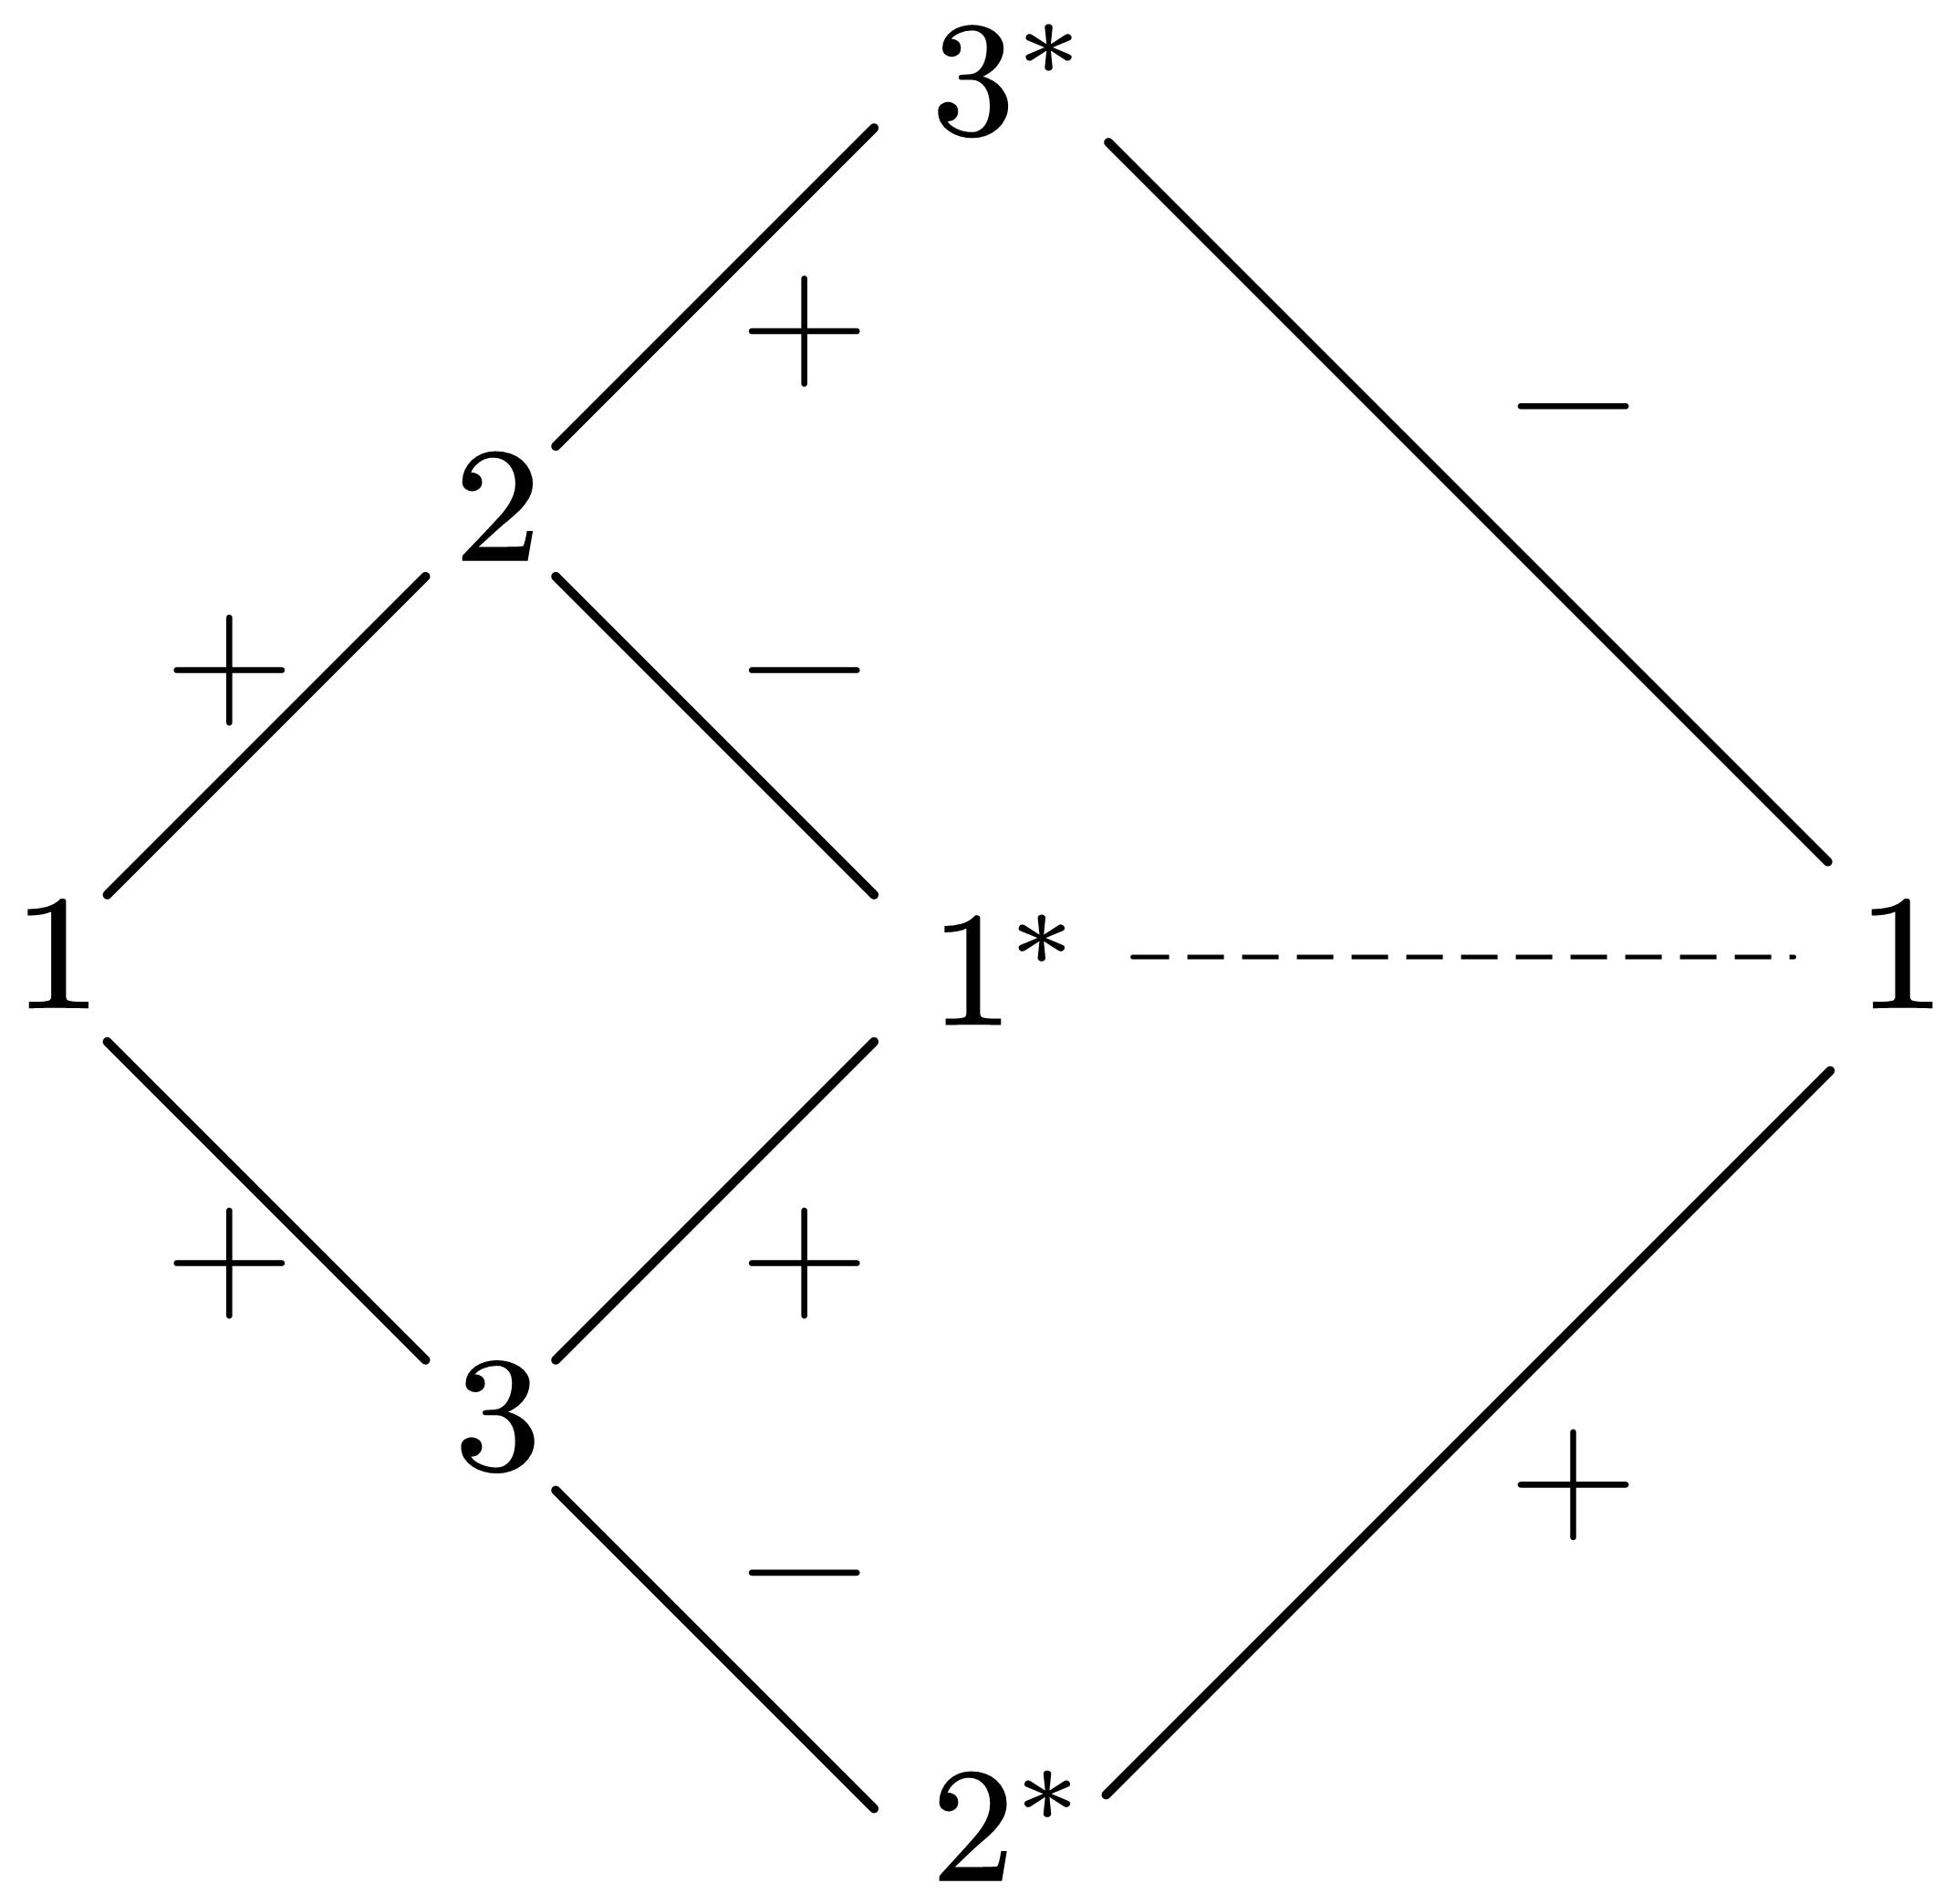
\includegraphics[scale=0.8]{./pictures/6.05/pictorial_representation_1.png}
		\captionof{figure}{Pictorial representation of the second term in $E^{(3)}_0$, where the order is $v_{ij}$, $v_{jk^*}$ and $v_{k^*i}$ from the left to the right. The plus and minus signs indicate whether the matrix elements between the two orbitals is $\pm \frac{\beta}{2}$.}\label{fig:exe5}
	\end{center}
	
	With the high symmetry, it is
	\begin{sequation}
		-2 \times \frac{1}{ (2\beta)^2 } \sum_{i=1}^3 \left[ v_{12} v_{23^*} v_{3^*1} + v_{13} v_{32^*} v_{2^*1} \right] = - \frac{3}{ 2\beta^2 } \left[ \frac{ \beta }{2} \times \frac{ \beta }{2} \times \left( - \frac{ \beta }{2} \right) + \frac{ \beta }{2} \times \left( - \frac{ \beta }{2} \right) \times \frac{ \beta }{2} \right] = \frac{3}{8\beta} .
	\end{sequation}	
	
	\end{solution}

	% 6.6
	\begin{exercise}
	Consider a cyclic polyene with $N = 4\nu+2$, $\nu=1$, $2$, ... carbons. Instead of assuming that all the bonds are identical, suppose they alternate in length. In the context of H{\"u}ckel theory this means that the resonance integrals between adjacent carbons are not all equal to $\beta$ but alternate between $\beta_1$ and $\beta_2$. For example, for benzene we have
	
	\begin{center}
	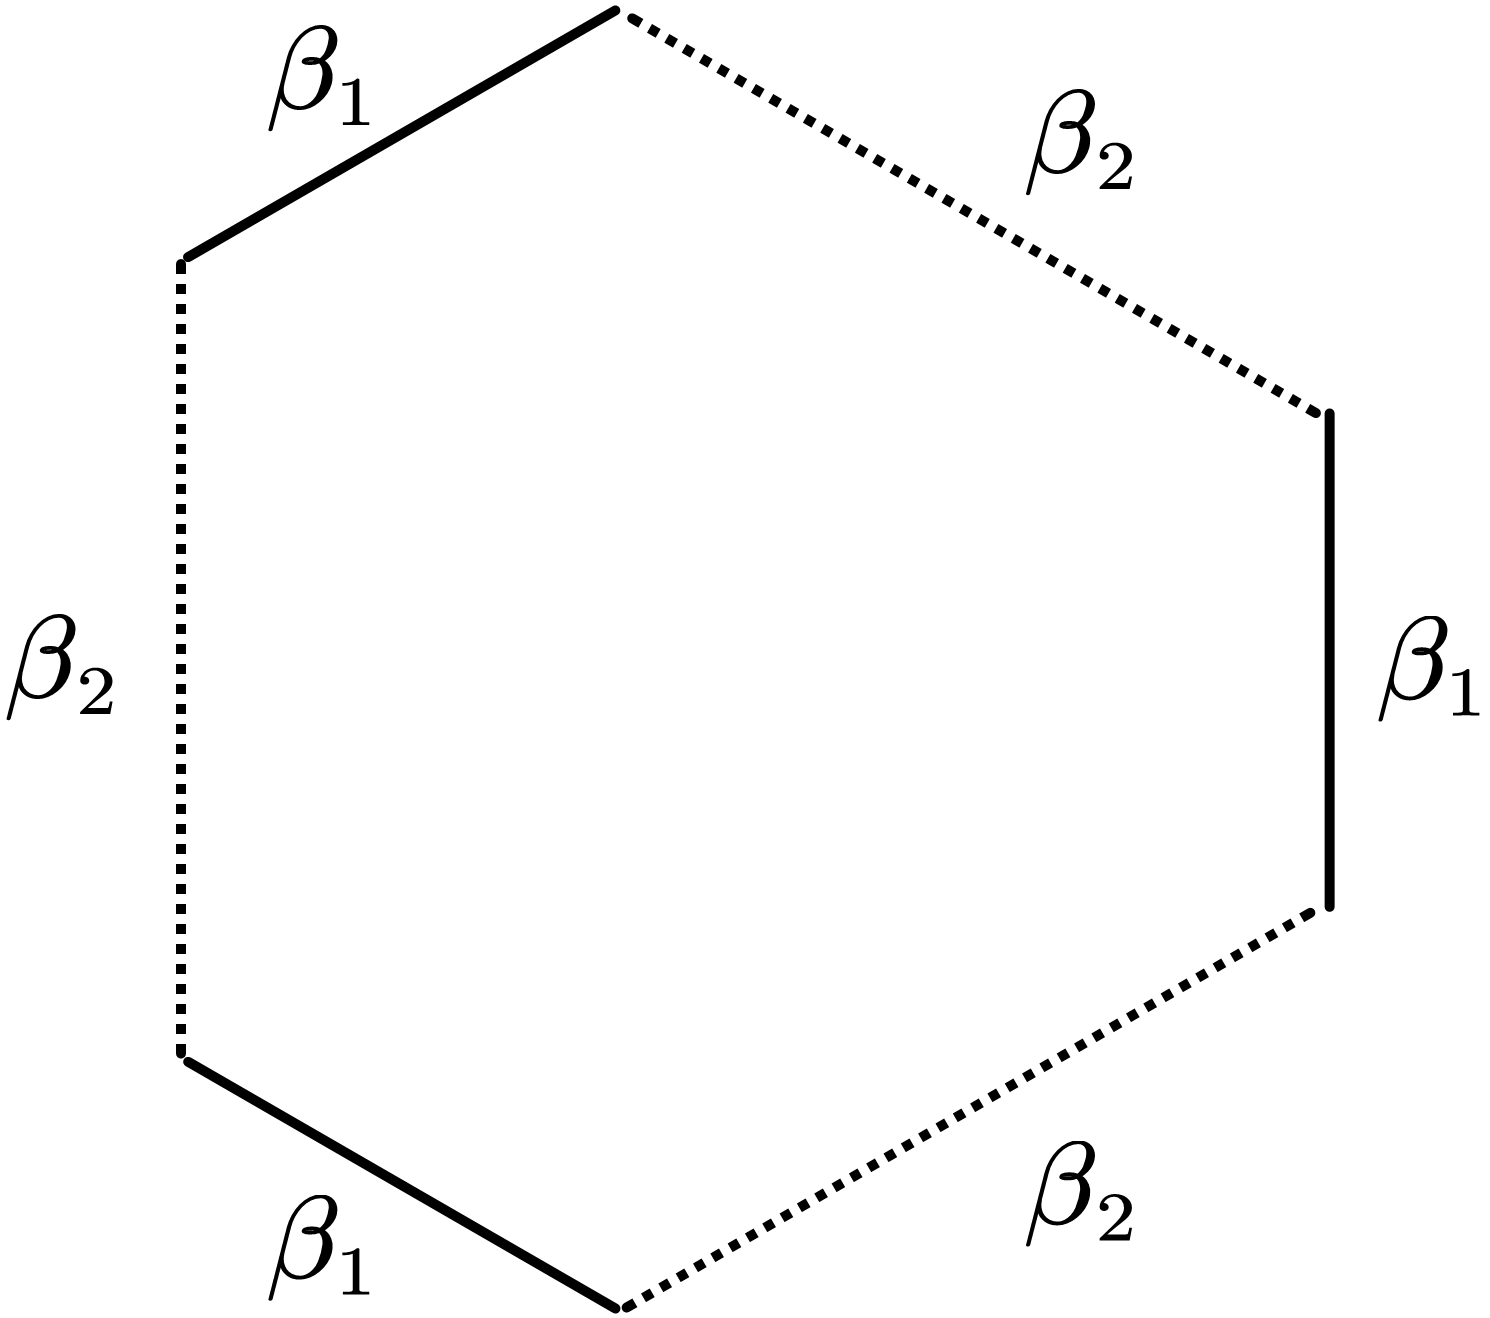
\includegraphics[scale=1.2]{./pictures/6.06/exercise_1.png}
	\end{center}
	
	Now it can be shown that the exact energy for a cyclic polyene of this type is
	\[
		\mathscr{E}_0 = N \alpha - 2 \sum_{j=-\nu}^\nu \left( \beta^2_1 + \beta^2_2 + 2 \beta_1 \beta_2 \cos{\frac{2j\pi}{2\nu+1}} \right)^{1/2}
	\]
	(see for example, L. Salem, {\it Molecular Orbital Theory of Conjugated Systems}, Benjamin, New York, 1966, pp.498-500). Note that when $\beta_1 = \beta_2 = \beta$, since $2\cos^2\theta=(1+\cos2\theta)$ and $\beta$ is negative, we recover
	\[
		\mathscr{E}_0 = N \alpha + 4 \beta \sum_{j=-\nu}^\nu \cos{\frac{j\pi}{2\nu+1}}
	\]
	which is the result quoted in Subsection 5.3.2. Also note that when $\beta_1=\beta$ but $\beta_2=0$, we have
	\[
		\mathscr{E}_0 = N \alpha + N \beta
	\]
	which is just the total energy of the polyene using the localized ethylenic description. The purpose of this exercise is to obtain the perturbation expansion for the resonance energy by expanding the exact energy in powers of $\beta_2/\beta_1$.
	\begin{enumerate}
	
	\item[a.] Show that for benzene ($\nu=1$) the exact ground state energy in the alternating short and long bond model is
	\[
		\mathscr{E}_0 = 6 \alpha + 2(\beta_1 + \beta_2) - 4 ( \beta^2_1 + \beta^2_2 - \beta_1 \beta_2 )^{1/2}
	\]
	Do this first by using the general expression and then by setting up the H{\"u}ckel matrix, diagonalizing it and adding up the occupied orbital energies. Note that when $\beta_1=\beta_2=\beta$ we recover our old result, $6\alpha+8\beta$.
	
	\item[b.] Setting $\beta_1 = \beta$ and $\beta_2/\beta_1=x$ show that the resonance energy of benzene can be written as
	\[
		E_R = 4 \beta ( \frac{1}{2}x - 1 + (1-x+x^2)^{1/2})
	\]
	Note that when $x=0$, $E_R=0$ and when $x=1$, $E_R=2\beta$ which is exact.
	
	\item[c.] Using the relation
	\[
		(1 + y)^{1/2} = 1 + \frac{1}{2} y - \frac{1}{8}y^2 + \frac{1}{16} y^3 - \frac{5}{128}y^4 + \cdots , \quad |y|<1
	\]	
	expand $E_R$ to fourth order in $x$ and thus show that
	\[
		E_R = \beta ( \frac{3}{2}x^2 + \frac{3}{4} x^3 + \frac{3}{32}x^4 + \cdots )
	\]
	Identifying the coefficient of $x^n$ with the $n$th-order perturbation result (i.e., $E^{(n)}_0$), we have
	\begin{align*}
		E^{(2)}_0 &= \frac{3}{2} \beta, \\
		E^{(3)}_0 &= \frac{3}{4} \beta, \\
		E^{(4)}_0 &= \frac{3}{32} \beta.
	\end{align*}
	Note that $E^{(2)}_0$ and $E^{(3)}_0$ agree with our previously calculated values. This derivation provides some insight into the poor convergence of the perturbation expansion of the resonance energy of benzene. Basically, the perturbation expansion converges rapidly when $x$ is small. However, for our problem $x$ is equal to unity.
	
	The resonance energy calculated up to $M$th-order as a function of $M$ is shown below. Note the oscillatory convergence towards the exact value of $2\beta$. The method used above to obtain $E^{(n)}_0$ for $n=2,3,4$ becomes extremely laborious for larger $n$. The results below were calculated by first showing that $E^{(n)}_0 = 4\beta C^{-1/2}_n(1/2)$, where $C^{-1/2}_n(x)$ is a Gegenbauer polynomial of degree $n$ and order $-\frac{1}{2}$, and then using the recursive properties of these polynomials, to show that
	\[
		(n+1)E^{(n+1)}_0 = (n-1) E^{(n)}_0 - (n-2) E^{(n-1)}_0.
	\]
	
	\begin{center}
	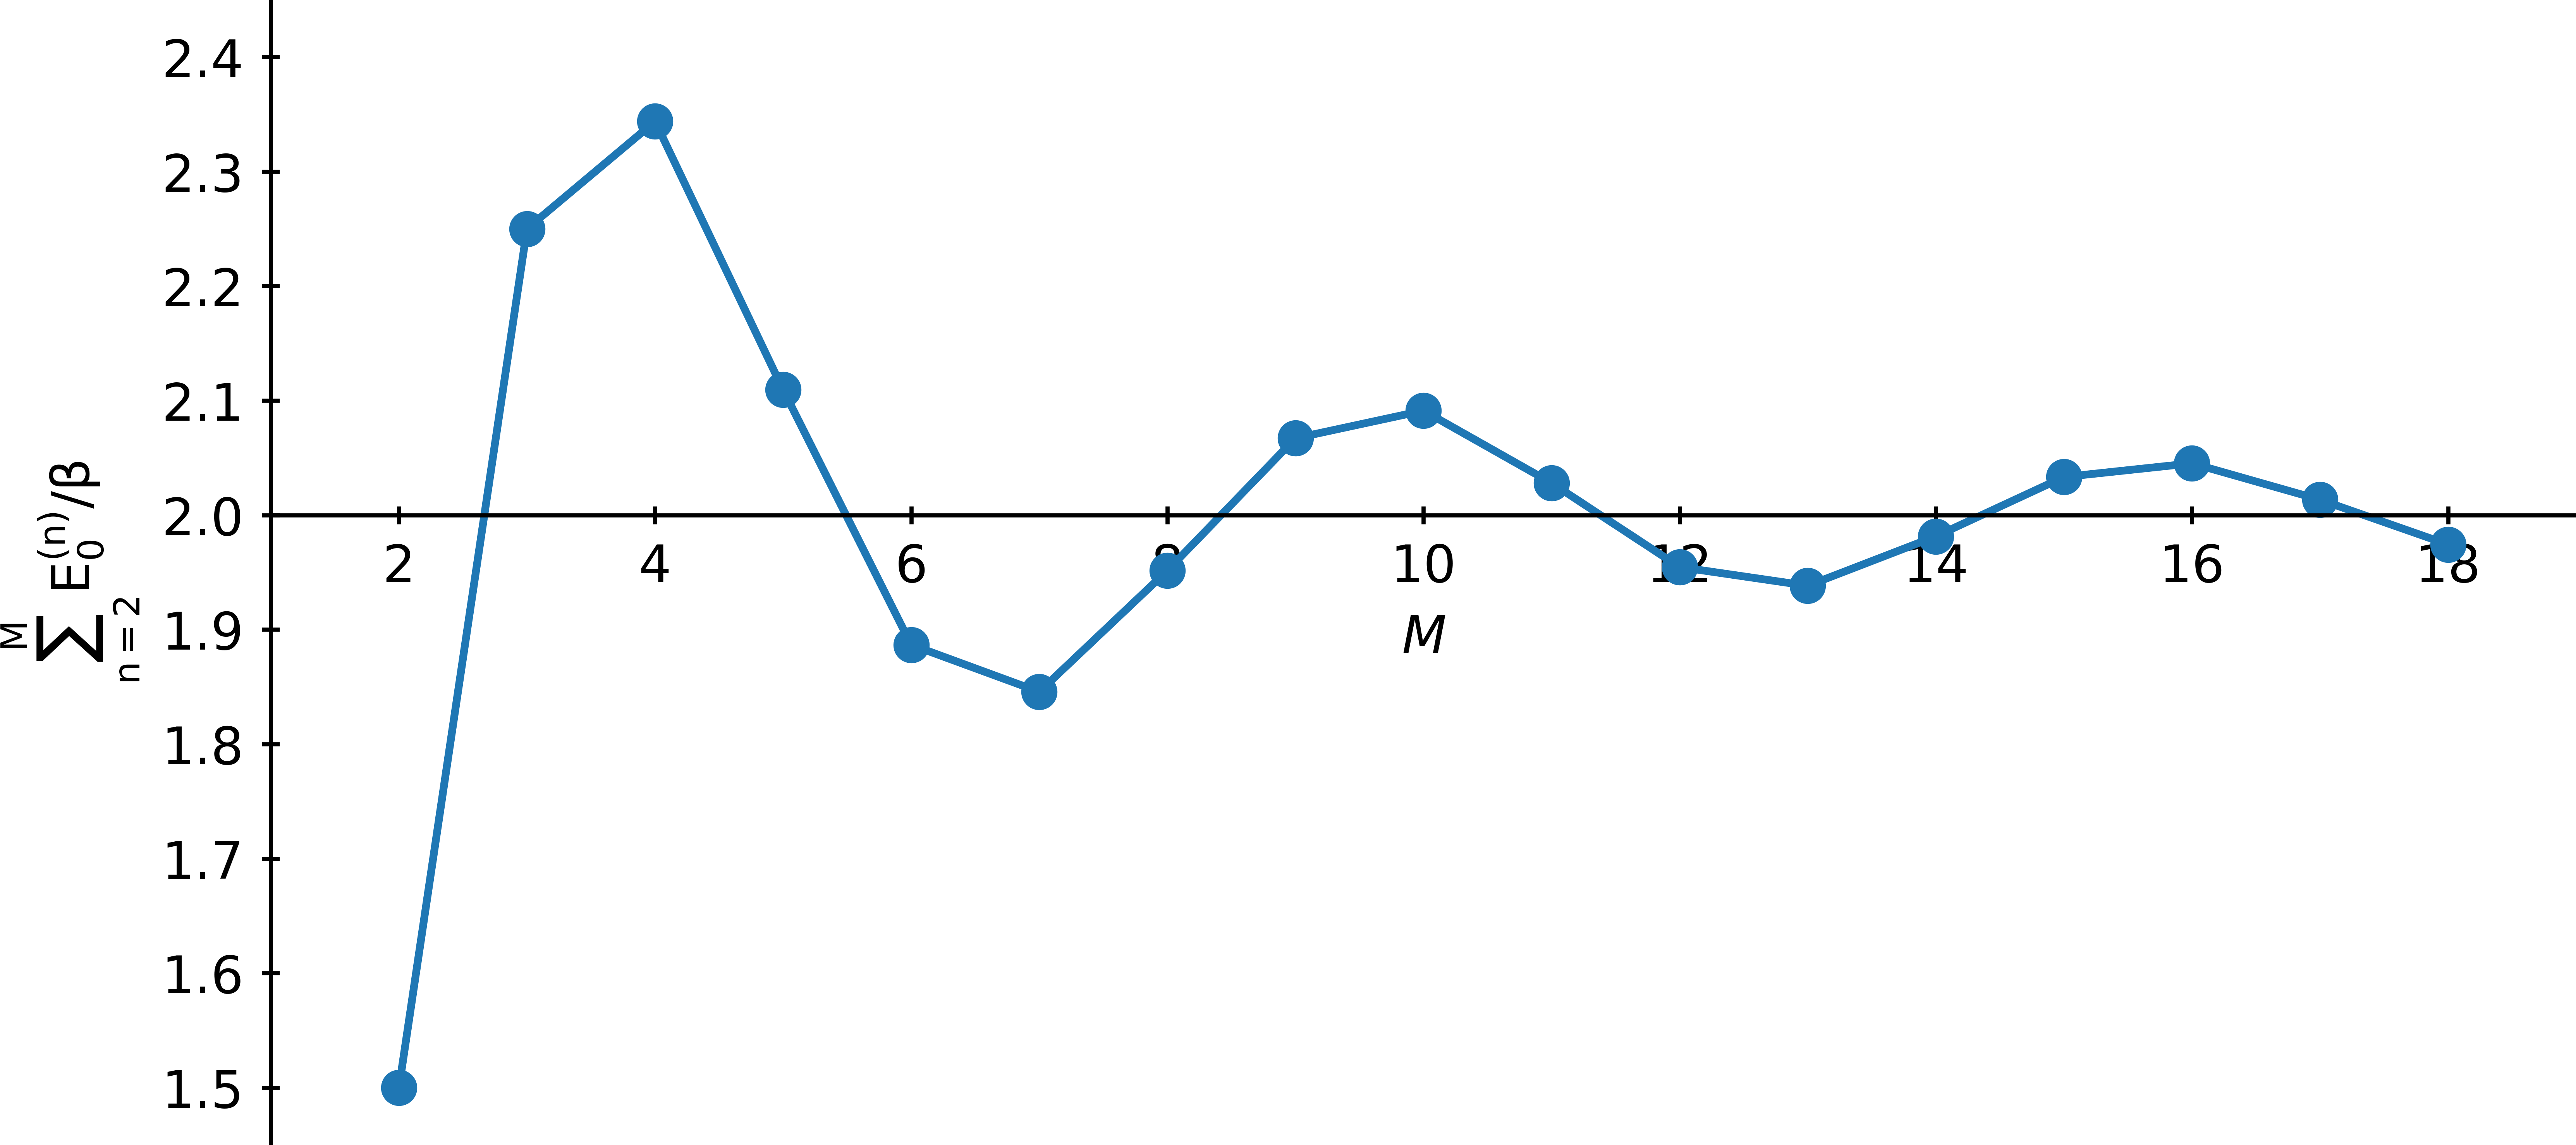
\includegraphics[scale=0.84]{./pictures/6.06/gegenbauer.png}
	\end{center}
	
	\end{enumerate}
	
	\end{exercise}
	
	\begin{solution}

	\begin{itemize}
	
	\item[a.] Using the general expression and note that $\beta_1 \le 0$ and $\beta_2 \le 0$, we get that
	\begin{align*}
		\mathscr{E}_0({\rm benzene}) &= 6 \times \alpha - 2 \sum_{ j=-1 }^1 \left( \beta^2_1 + \beta^2_2 + 2 \beta_1 \beta_2 \cos{\frac{2j\pi}{ 2 \times 1 + 1 }} \right)^{1/2} \\
		&= 6\alpha - 2 \left( \beta^2_1 + \beta^2_2 + 2 \beta_1 \beta_2 \cos{\frac{-2\pi}{ 3 }} \right)^{1/2} \\
		&\hspace{2em} - 2 \left( \beta^2_1 + \beta^2_2 + 2 \beta_1 \beta_2 \cos{\frac{0\pi}{ 3 }} \right)^{1/2} - 2 \left( \beta^2_1 + \beta^2_2 + 2 \beta_1 \beta_2 \cos{\frac{2\pi}{ 3 }} \right)^{1/2} \\
		&= 6\alpha - 2\left( \beta^2_1 + \beta^2_2 - \beta_1 \beta_2 \right)^{1/2} + 2\left( \beta_1 + \beta_2 \right) - 2\left( \beta^2_1 + \beta^2_2 - \beta_1 \beta_2 \right)^{1/2}.
	\end{align*}
	In a nut shell,
	\begin{sequation}
		\mathscr{E}_0({\rm benzene}) = 6\alpha + 2\left( \beta_1 + \beta_2 \right) - 4\left( \beta^2_1 + \beta^2_2 - \beta_1 \beta_2 \right)^{1/2} .
	\end{sequation}
	
	At this time, we should remember that the H{\"u}ckel matrix is 
	\[
		\HH = \begin{pmatrix}
			\alpha & \beta_2 & 0 & 0 & 0 & \beta_1 \\
			\beta_2& \alpha  & \beta_1 & 0 & 0 & 0 \\
			0 & \beta_1& \alpha  & \beta_2 & 0 & 0 \\
			0 & 0 & \beta_2& \alpha  & \beta_1 & 0 \\
			0 & 0 & 0 & \beta_1& \alpha  & \beta_2 \\
			\beta_1 & 0 & 0 & 0 & \beta_2 & \alpha
		\end{pmatrix}.
	\]
	Its eigen function is
	\[
		\det{\HH-\varepsilon\I} = (\beta^2_1 - \beta_1 \beta_2 + \beta^2_2 - (\alpha - \varepsilon)^2)^2 (\alpha - \beta_1 - \beta_2 - \varepsilon) (\alpha + \beta_1 + \beta_2 - \varepsilon) = 0,
	\]
	and there are six roots:
	\begin{align*}
		\varepsilon_1 &= \alpha + \beta_1 + \beta_2 , \\
		\varepsilon_2 = \varepsilon_3 &= \alpha - \sqrt{ \beta^2_1 - \beta_1 \beta_2 + \beta^2_2 }, \\
		\varepsilon_4 = \varepsilon_5 &= \alpha + \sqrt{ \beta^2_1 - \beta_1 \beta_2 + \beta^2_2 }, \\
		\varepsilon_6 &= \alpha - \beta_1 - \beta_2 .
	\end{align*}
	Thus,
	\begin{sequation}
		\mathscr{E}^\prime_0({\rm benzene}) = 2\varepsilon_1 + 2\varepsilon_2 + 2\varepsilon_3 = 6\alpha + 2\left( \beta_1 + \beta_2 \right) - 4\left( \beta^2_1 + \beta^2_2 - \beta_1 \beta_2 \right)^{1/2} .
	\end{sequation}
	It equals the results obtained by using the general expression.
	
	\item[b.] The verification is direct. With $\beta_1 = \beta$, $\beta_2 = x\beta_1 = x\beta$, we get that
	\begin{align*}
		E_R &= \mathscr{E}_0({\rm benzene}) - E_0 = 6\alpha + 2\left( \beta + x \beta \right) - 4\left( \beta^2 + ( x \beta )^2 - x \beta^2 \right)^{1/2} - ( 6\alpha + 6\beta ) \\
		&= -4\beta + 2x \beta + 4\beta \left( 1 + x^2 - x \right)^{1/2} = 4\beta \left( \frac{x}{2} - 1 + \left( 1 + x^2 - x \right)^{1/2} \right)
	\end{align*}
	
	\item[c.] When $0 \le x \le 1$, $-\frac{1}{4} \le x^2-x \le 0$, thus we obtain that
	\begin{align*}
		E_R &= 4\beta \left( \frac{x}{2} - 1 + \left( 1 + x^2 - x \right)^{1/2} \right) = 4\beta \left[ \frac{x}{2} - 1 + \left( 1 + \left( x^2 - x \right) \right)^{1/2} \right] \\
		&= 4\beta \left[ \frac{x}{2} - 1 + 1 + \frac{1}{2} \left( x^2 - x \right) - \frac{1}{8} \left( x^2 - x \right)^2 + \frac{1}{16} \left( x^2 - x \right)^3 - \frac{5}{128} \left( x^2 - x \right)^4 + \cdots \right] \\
		&= 4\beta \left[ \frac{x}{2} + \frac{1}{2} \left( - x + x^2 \right) - \frac{1}{8} \left( x^2 - 2 x^3 + x^4 \right)  \right. \\
		&\hspace{4em} \left. + \frac{1}{16} \left( - x^3 + 3 x^4 - 3 x^5 + x^6 \right) - \frac{5}{128} \left( x^4 - 4x^5 + 6x^6 - 4x^7 + x^8 \right) + \cdots \right] \\
		&= 4\beta \left[ \left( \frac{1}{2} - \frac{1}{2} \right) x + \left( \frac{1}{2} - \frac{1}{8} \right) x^2 + \left( \frac{1}{4} - \frac{1}{16} \right) x^3 + \left( - \frac{1}{8} + \frac{3}{16} - \frac{5}{128} \right) x^4 + \cdots \right] \\
		&= \beta \left( \frac{3}{2} x^2 + \frac{3}{4} x^3 + \frac{3}{32} x^4 + \cdots \right) .
	\end{align*}
	
	In fact, the Gegenbauer polynomials $C^\lambda_n(x)$ can be generated by $(1-2xt+t^2)^{-\lambda}$, viz.,
	\[
		(1-2xt+t^2)^{-\lambda} = \sum_{ n=0 }^\infty C^\lambda_n (x) t^n, \, \forall t \in (-1,1), x \in (-1,1).
	\]
	Let $\lambda=-\frac{1}{2}$ and $x=\frac{1}{2}$, we obtain that
	\[
		( 1 - t + t^2 )^{\frac{1}{2}} = \sum_{ n=0 }^\infty C^{-\frac{1}{2}}_n \left( \frac{1}{2} \right) t^n.
	\]
	Thus, with 
	\[
		C^\lambda_0(x) = 1 , \quad C^\lambda_1(x) = 2 \lambda x ,
	\]	
	we find that	
	\[
		\sum_{ n=0 }^\infty C^{-\frac{1}{2}}_n \left( \frac{1}{2} \right) t^n = C^{-\frac{1}{2}}_0 \left( \frac{1}{2} \right) + C^{-\frac{1}{2}}_0 \left( \frac{1}{2} \right) t + \sum_{ n=2 }^\infty C^{-\frac{1}{2}}_n \left( \frac{1}{2} \right) t^n = 1 - \frac{t}{2} + \sum_{ n=2 }^\infty C^{-\frac{1}{2}}_n \left( \frac{1}{2} \right) t^n.
	\]
	
	Hence, we get
	\begin{sequation}
		E_R = 4\beta \left( \frac{x}{2} - 1 + \left( 1 - x + x^2 \right)^{1/2} \right) = 4\beta \sum_{ n=2 }^\infty C^{-\frac{1}{2}}_n \left( \frac{1}{2} \right) x^n.
	\end{sequation}
	It equals
	\begin{sequation}
		E^{(n)}_0 = 4\beta C^{-\frac{1}{2}}_n \left( \frac{1}{2} \right), \, n = 2, 3, 4, \cdots.
	\end{sequation}
	
	Due to the recurrence relation of Gegenbauer polynomials,
	\[
		(n+1)C^\lambda_{n+1}(x) = 2(n+\lambda) x C^\lambda_n(x) - ( n + 2\lambda - 1 ) C^\lambda_{n-1}(x), \, \forall n \ge 1, 
	\]
	we know that for $n=2,3,\cdots$,
	\begin{align*}
		(n+1)E^{(n+1)}_0 &= (n+1) \times 4\beta C^{-\frac{1}{2}}_{n+1} \left( \frac{1}{2} \right) = 4\beta (n+1) C^{-\frac{1}{2}}_{n+1} \left( \frac{1}{2} \right) \\
		&= 4\beta \left[ 2\left( n - \frac{1}{2} \right) \frac{1}{2} C^{ -\frac{1}{2} }_n \left( \frac{1}{2} \right) - \left( n + 2 \times \left( -\frac{1}{2} \right) - 1 \right) C^{ -\frac{1}{2} }_{n-1}\left( \frac{1}{2} \right) \right] \\
		&= 4\beta \left[ \left( n - \frac{1}{2} \right) C^{ - \frac{1}{2} }_n\left( \frac{1}{2} \right) - ( n - 2 ) C^{ - \frac{1}{2}}_{n-1}\left( \frac{1}{2} \right) \right] \\
		&= \left( n - \frac{1}{2} \right) 4\beta C^{ -\frac{1}{2} }_n\left( \frac{1}{2} \right) - ( n - 2 ) 4\beta C^{ -\frac{1}{2} }_{n-1}\left( \frac{1}{2} \right) \\
		&= \left( n - \frac{1}{2} \right) E^{(n)}_0 - ( n - 2 ) E^{(n-1)}_0.
	\end{align*}
	
	\end{itemize}
	
	Remark: You can read some introduction about Gegenbauer polynomials from WIKIPEDIA, whose url is \url{https://en.wikipedia.org/wiki/Gegenbauer_polynomials}.	
		
	\end{solution}
	
	\sectionstar{Diagrammatic Representation of Orbital Perturbation Theory}
	
	% 6.7
	\begin{exercise}
	Find the fourth-order energy for a closed-shell cyclic polyene.
	\begin{enumerate}
	
	\item[a.] Show that
	
	\begin{center}
	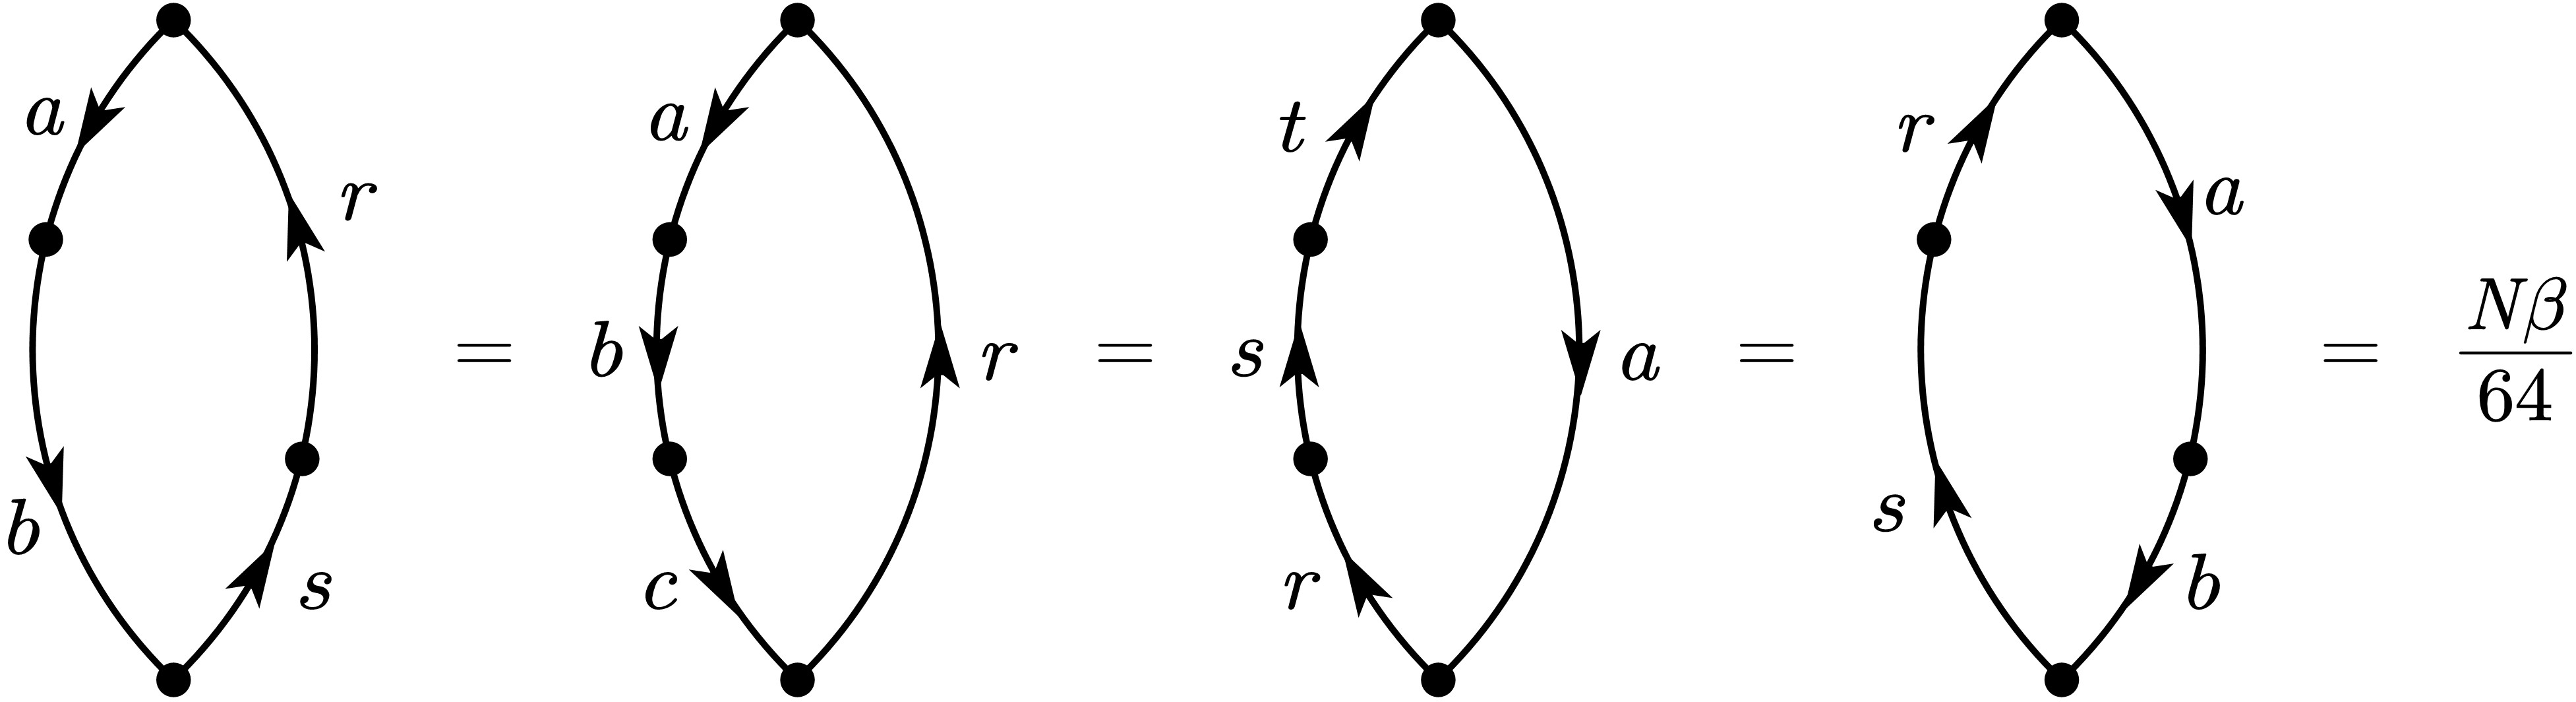
\includegraphics[scale=0.84]{./pictures/6.07/exercise_1.png}
	\end{center}
	
	and
	
	\begin{center}
	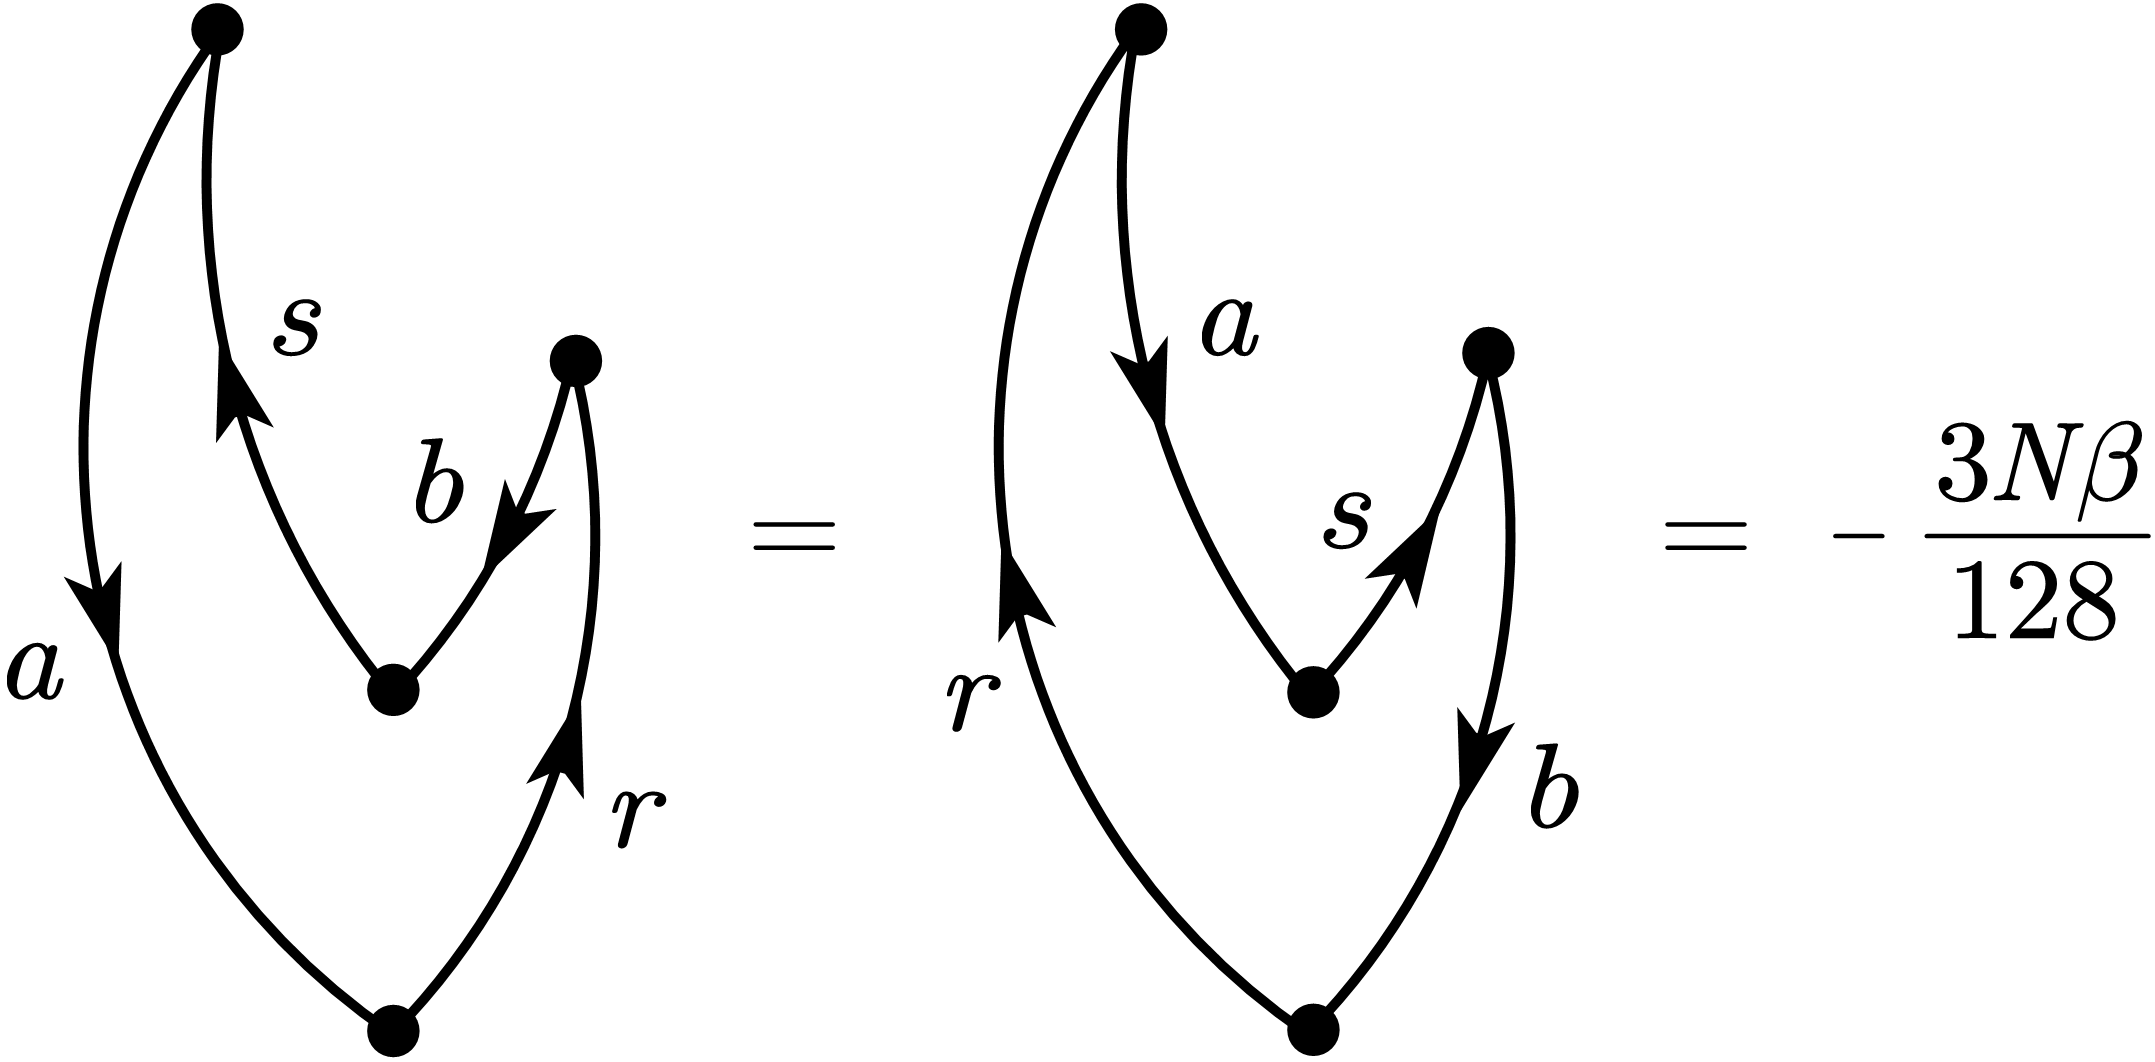
\includegraphics[scale=0.84]{./pictures/6.07/exercise_2.png}
	\end{center}
	
	so that
	\[
		E^{(4)}_0 = \frac{N\beta}{64}
	\]
	Thus the resonance energy calculated for a cyclic polyene with $N>6$ up to fourth order is (1/4 + 1/64)$N\beta = 0.2656N\beta$, which compares very favorably with the asymptotically exact value of 0.2732$\beta$ (i.e., 97\%).
	
	\item[b.] For benzene, show that the diagrammatic result for the fourth-order energy agrees with the independently calculated result found in Exercise 6.6.
	
	\end{enumerate}		
	
	\end{exercise}
	
	\begin{solution}
	
	\begin{itemize}	
	
	\item[a.] Firstly, we list all diagrams of the fourth-order energy. 	
	\begin{center}
	\begin{tabular}{ccc}
	
		\begin{minipage}{0.22\linewidth}
		\centering
		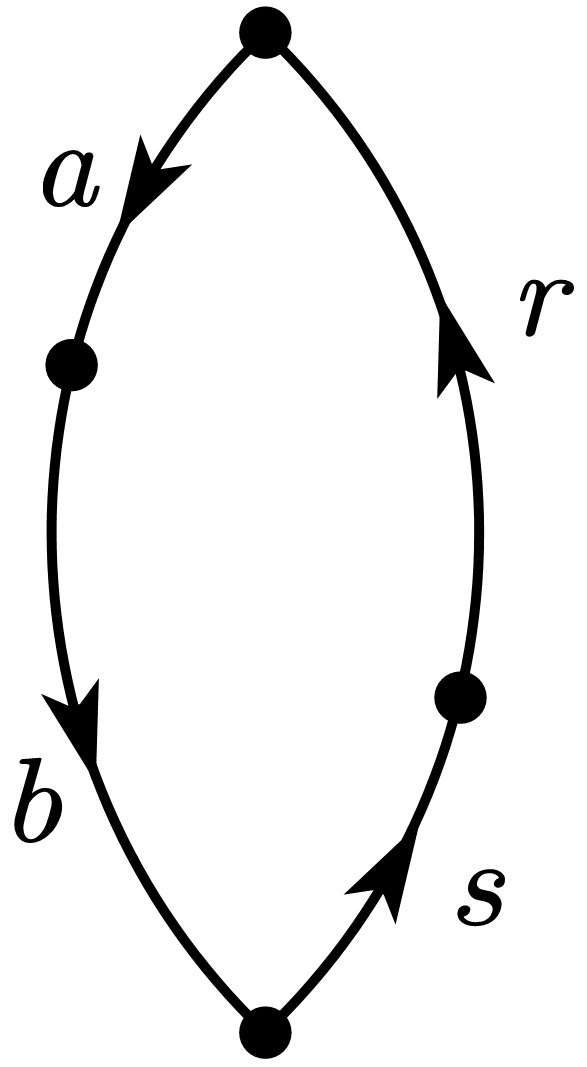
\includegraphics[scale=1.0,trim=0 -4 0 -4]{./pictures/6.07/diagram_1.png}
		\end{minipage} &
		
		\begin{minipage}{0.22\linewidth}
		\centering
		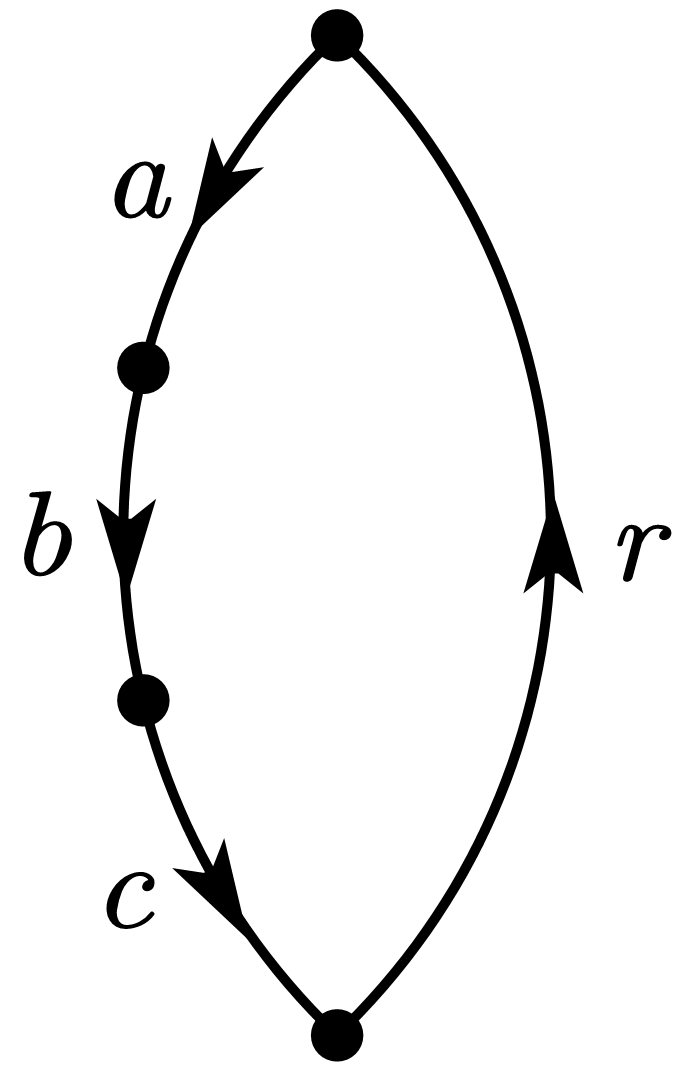
\includegraphics[scale=1.0,trim=0 -4 0 -4]{./pictures/6.07/diagram_2.png}
		\end{minipage} &
		
		\begin{minipage}{0.22\linewidth}
		\centering
		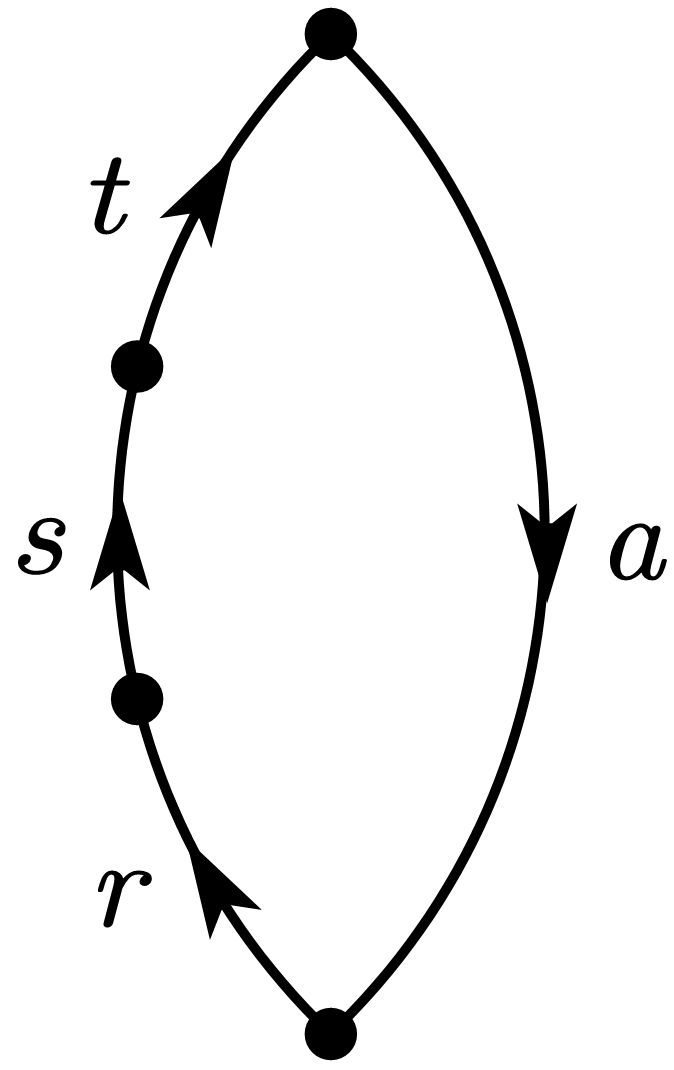
\includegraphics[scale=1.0,trim=0 -4 0 -4]{./pictures/6.07/diagram_3.png}
		\end{minipage} \\
		
		\begin{minipage}{0.22\linewidth}
		\centering
		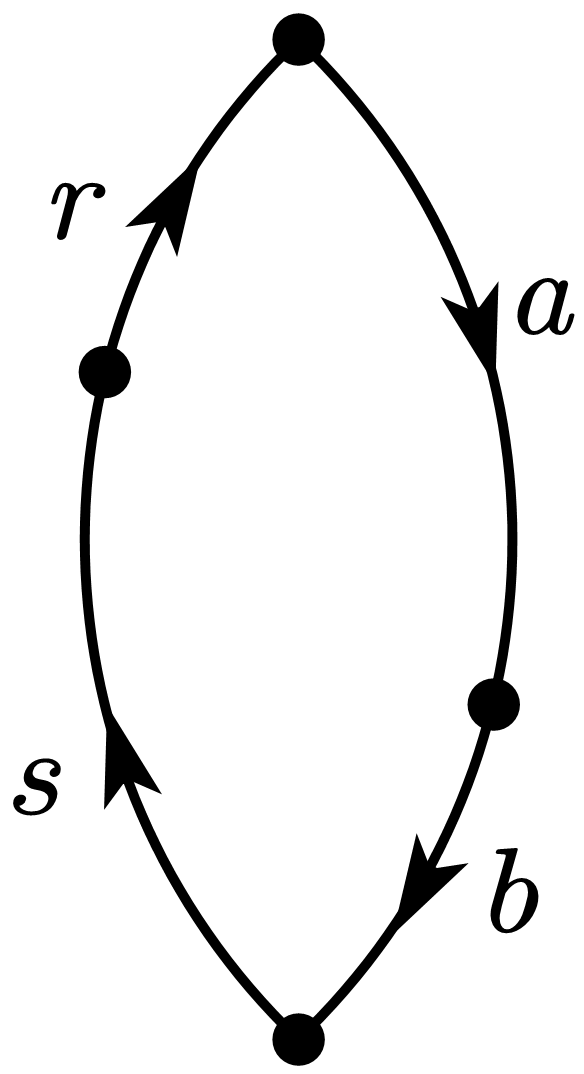
\includegraphics[scale=1.0,trim=0 -4 0 -4]{./pictures/6.07/diagram_4.png}
		\end{minipage} &
			
		\begin{minipage}{0.22\linewidth}
		\centering
		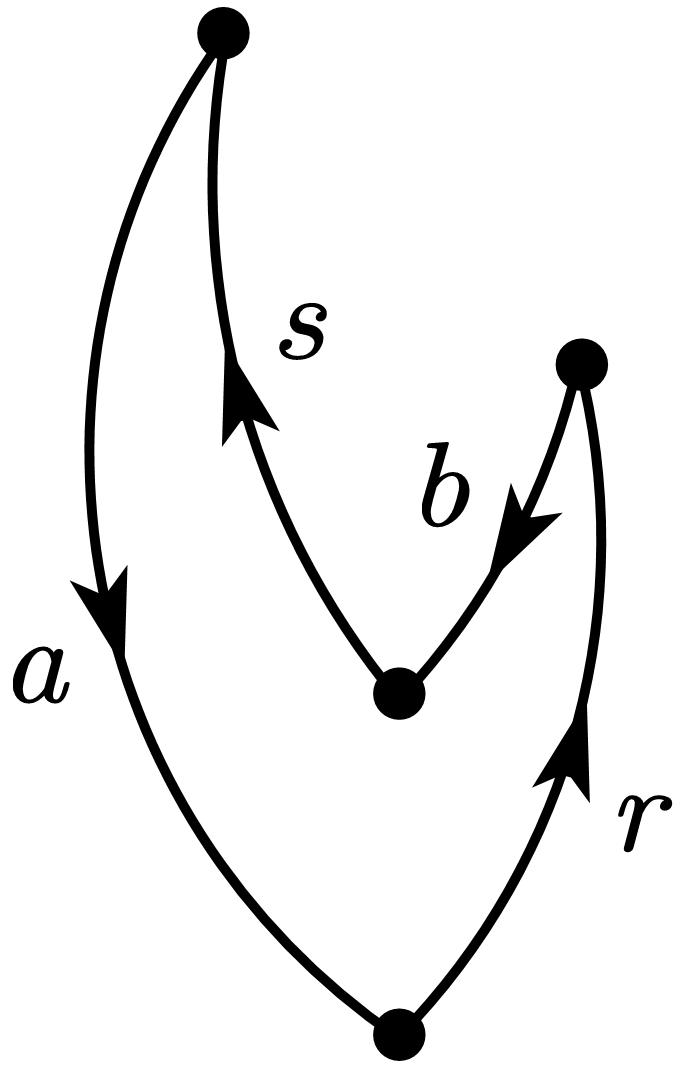
\includegraphics[scale=1.0,trim=0 -4 0 -4]{./pictures/6.07/diagram_5.png}
		\end{minipage} &
		
		\begin{minipage}{0.22\linewidth}
		\centering
		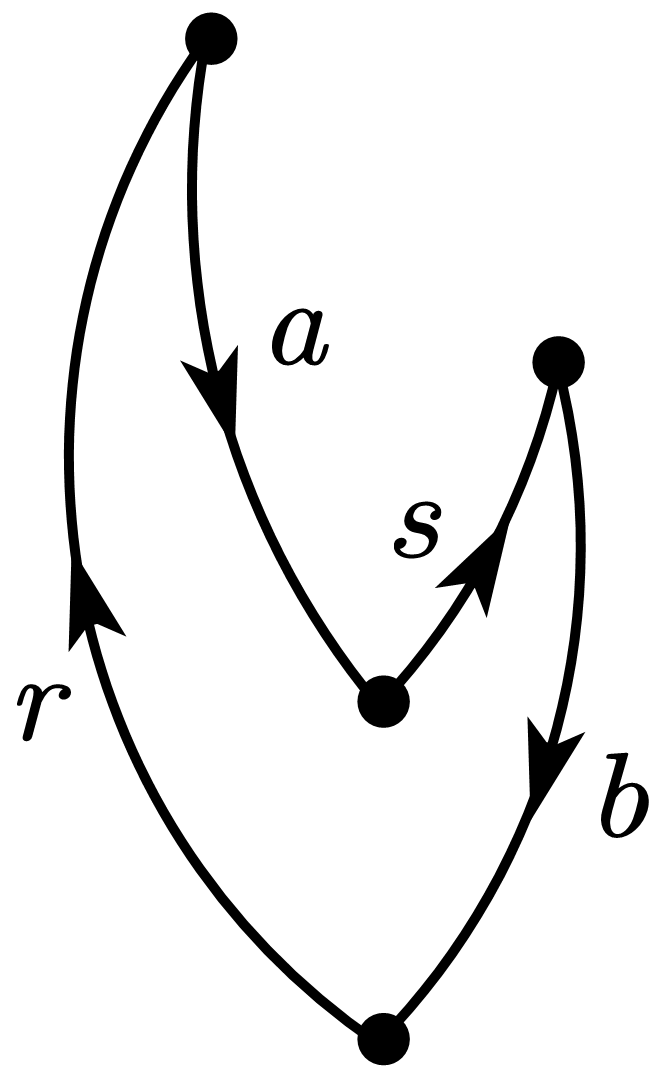
\includegraphics[scale=1.0,trim=0 -4 0 -4]{./pictures/6.07/diagram_6.png}
		\end{minipage}
		
	\end{tabular}
	\captionof{figure}{All fourth-order diagrams.}\label{fig:exe7_1}
	\end{center}
	
	Note that when $N>6$, $(i+3)^*$ cannot interact with $i$, and when $N=6$, $1^*$ cannot interact with $1$, either. Thus, there is no essential difference in the shape and properties between the case of $N > 6$ and $N=6$. It is enough to draw the pictorial representation of benzene ($N=6$) in order to get the same result of $N>6$. The pictorial representation of benzene can be seen in \Figref{fig:exe7_2}.
	
	\begin{center}
	\begin{tabular}{ccc}
	
		\begin{minipage}{0.3\linewidth}
		\centering
		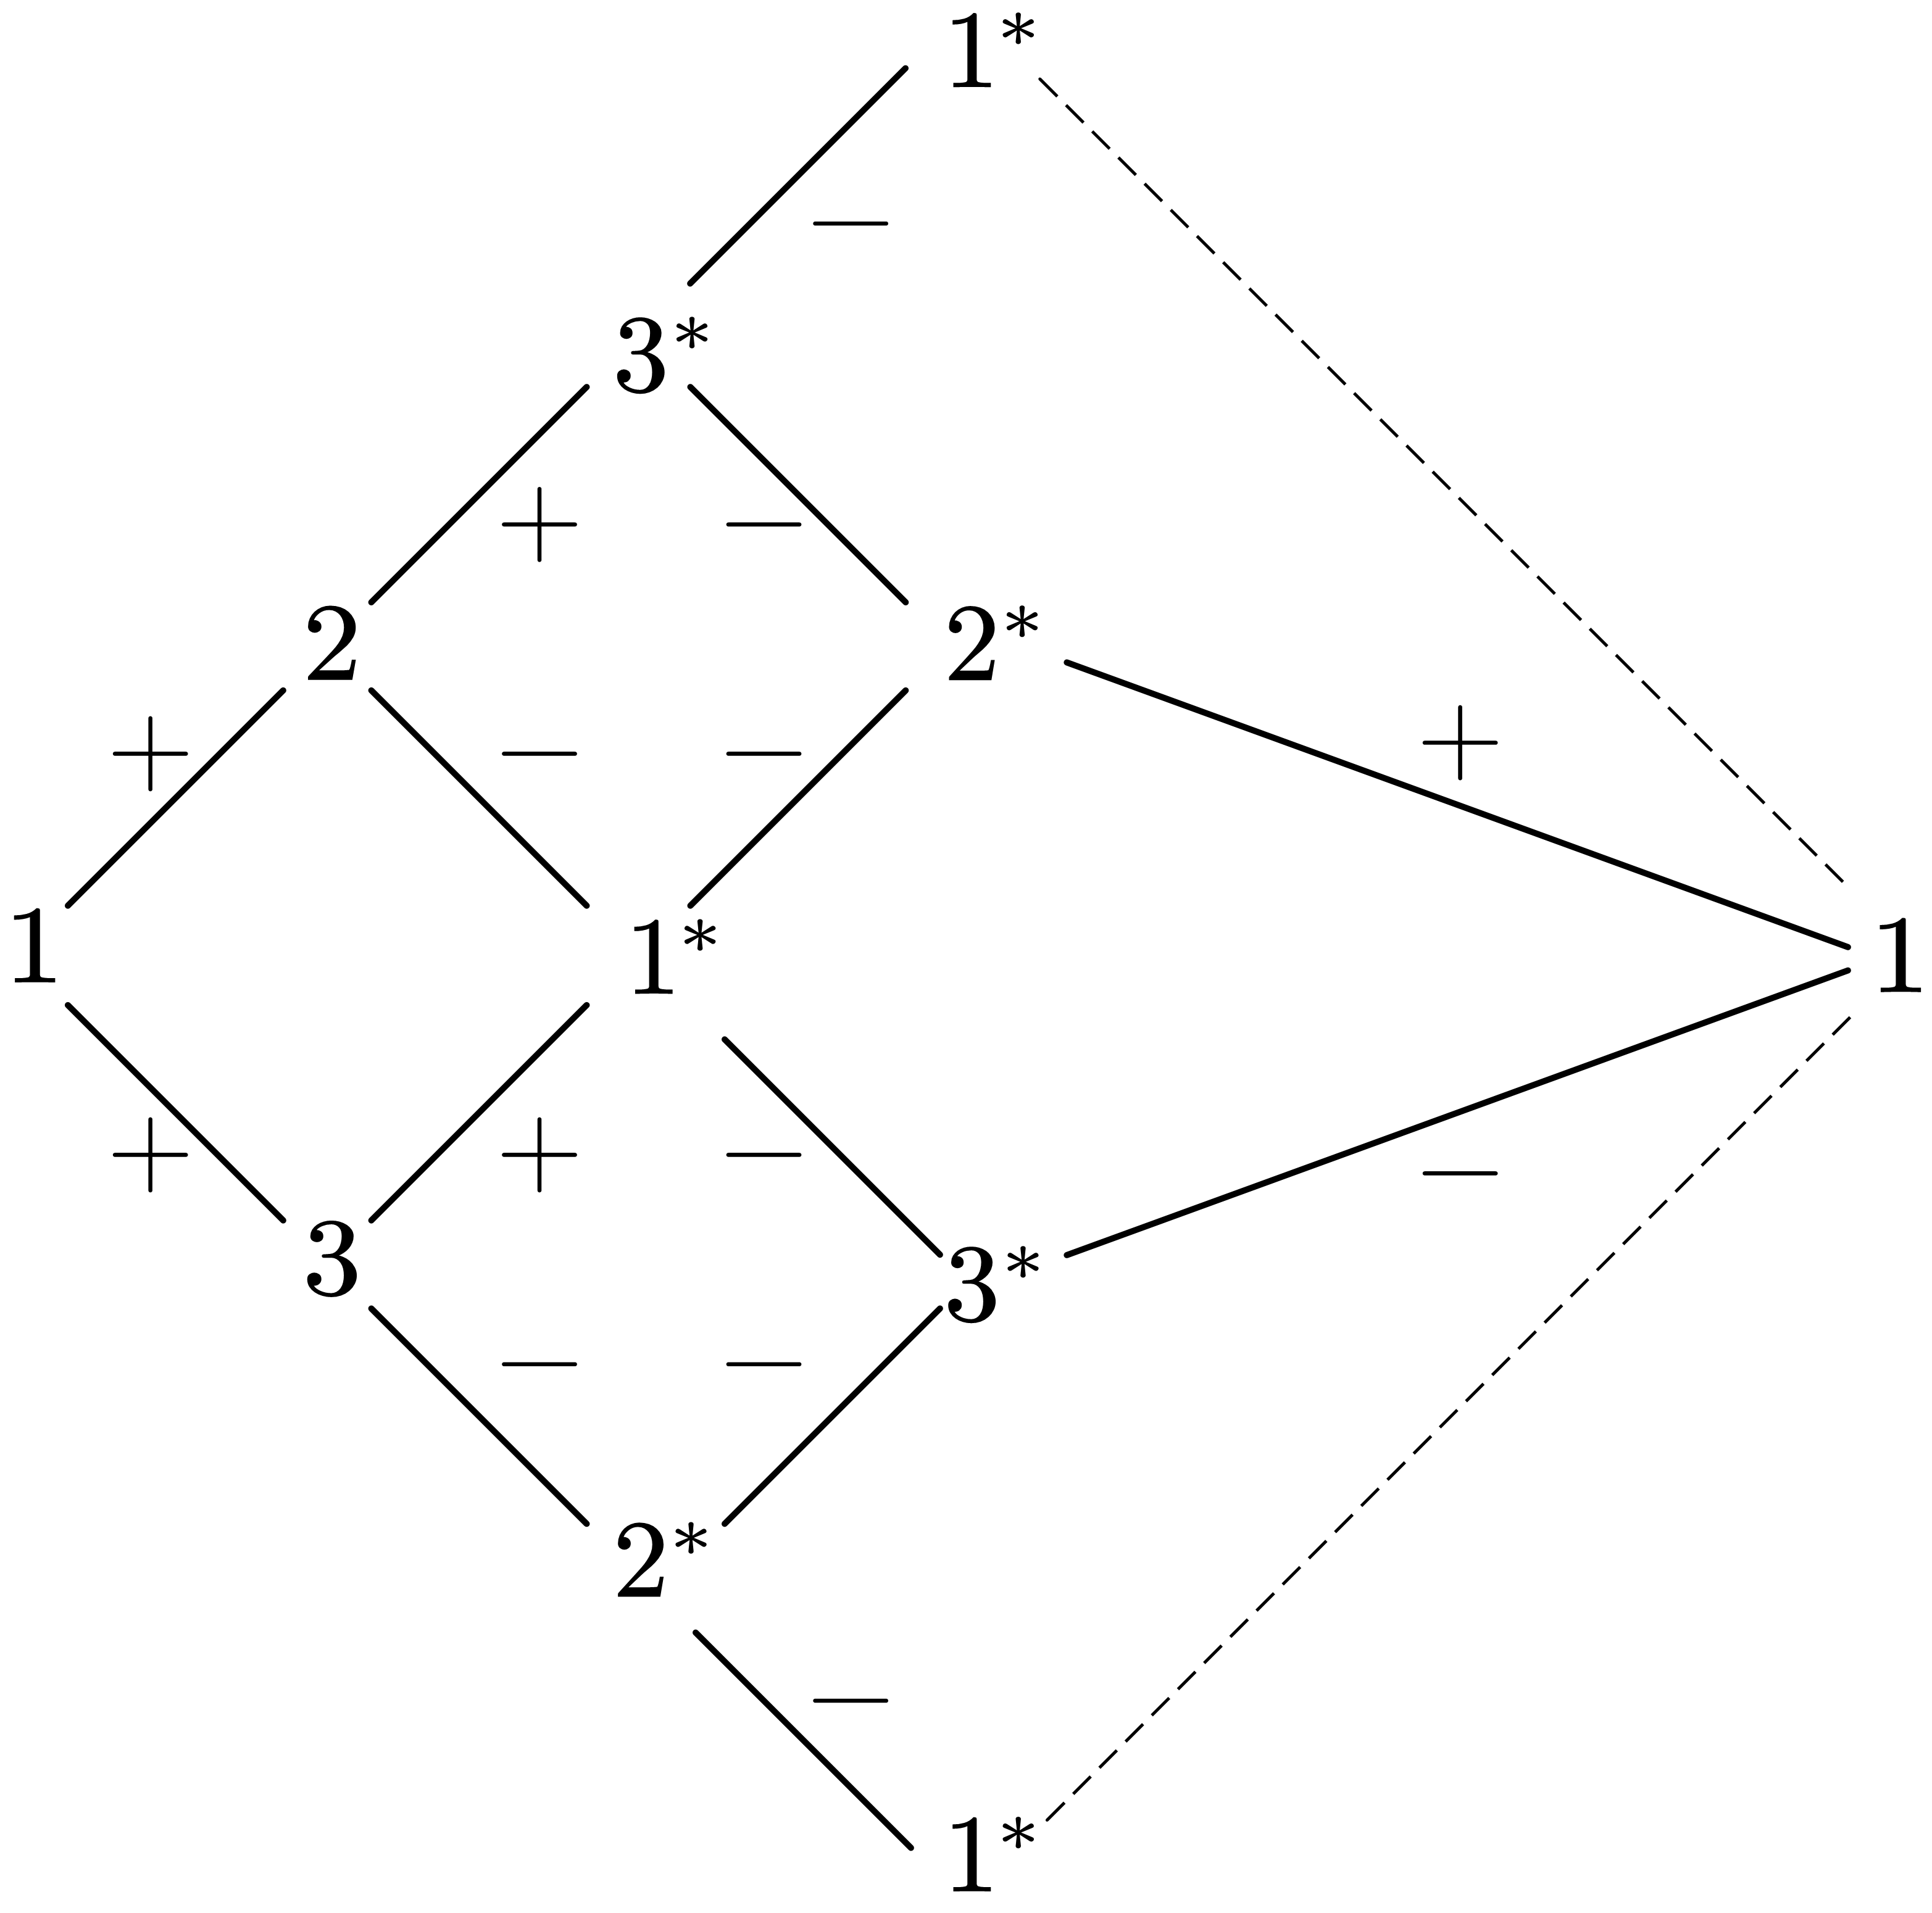
\includegraphics[scale=0.5,trim=0 -8 0 -8]{./pictures/6.07/pictorial_representation_1.png}
		\end{minipage} &
		
		\begin{minipage}{0.3\linewidth}
		\centering
		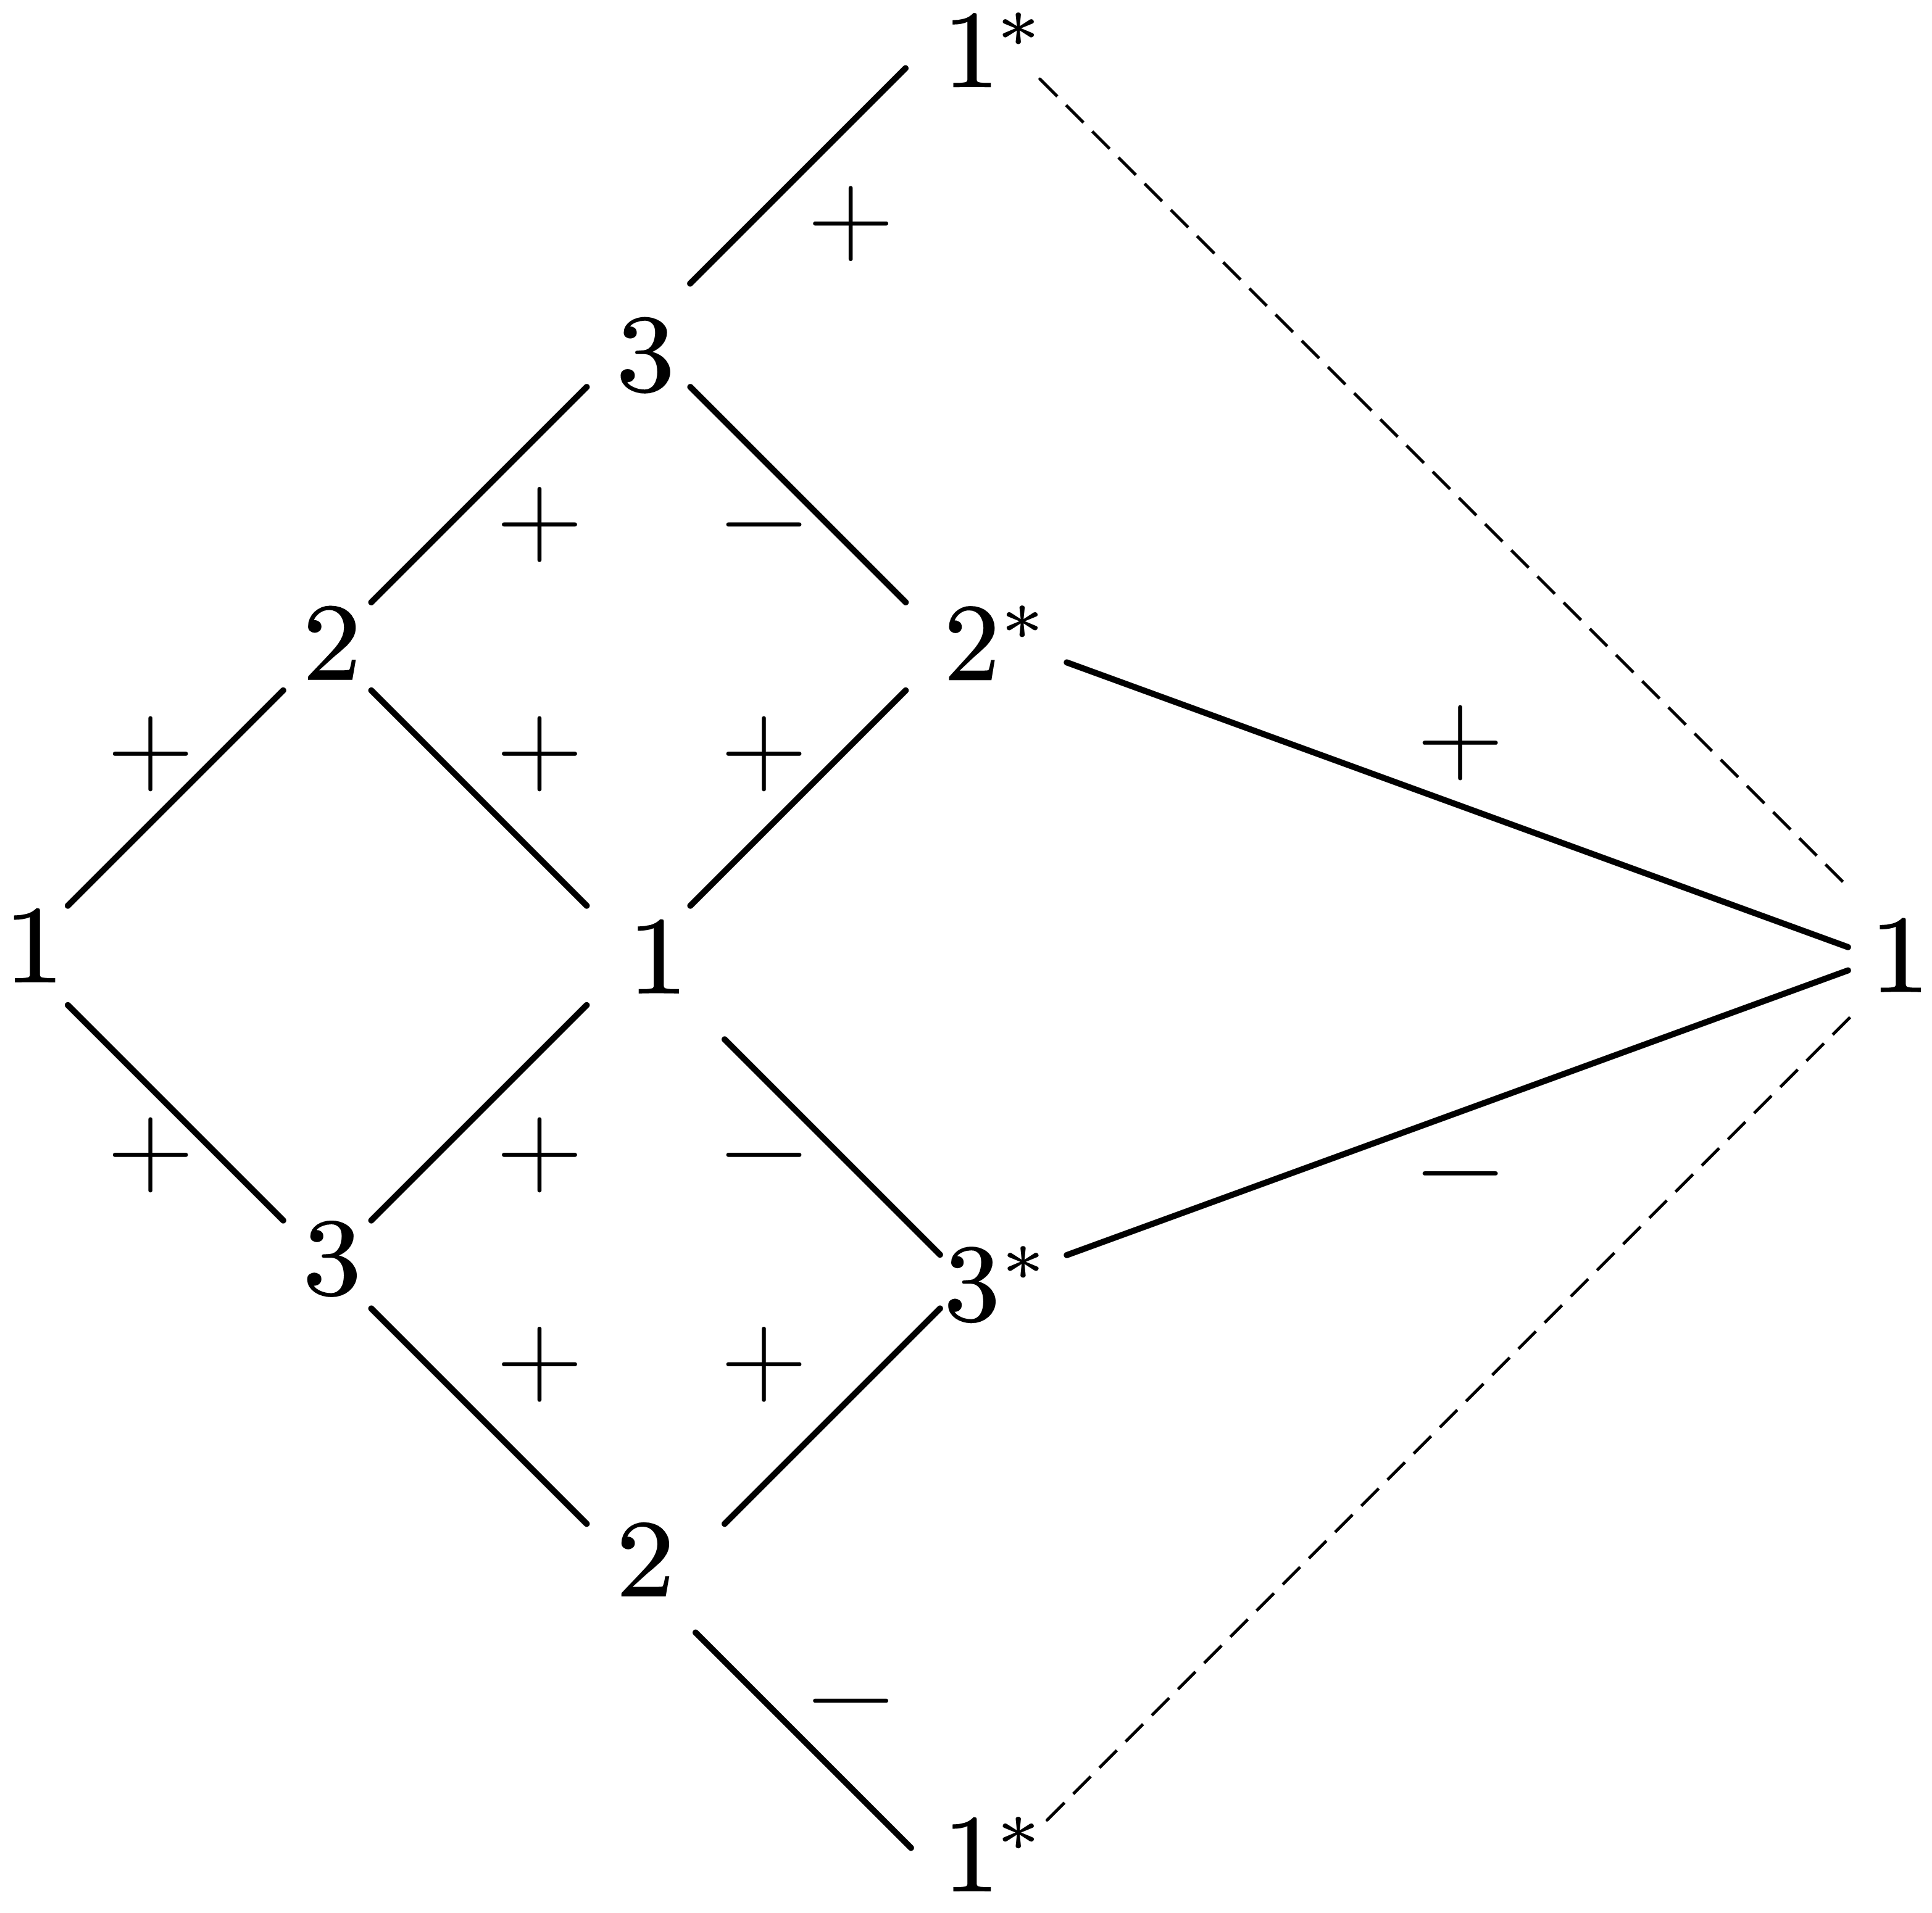
\includegraphics[scale=0.5,trim=0 -8 0 -8]{./pictures/6.07/pictorial_representation_2.png}
		\end{minipage} &
		
		\begin{minipage}{0.3\linewidth}
		\centering
		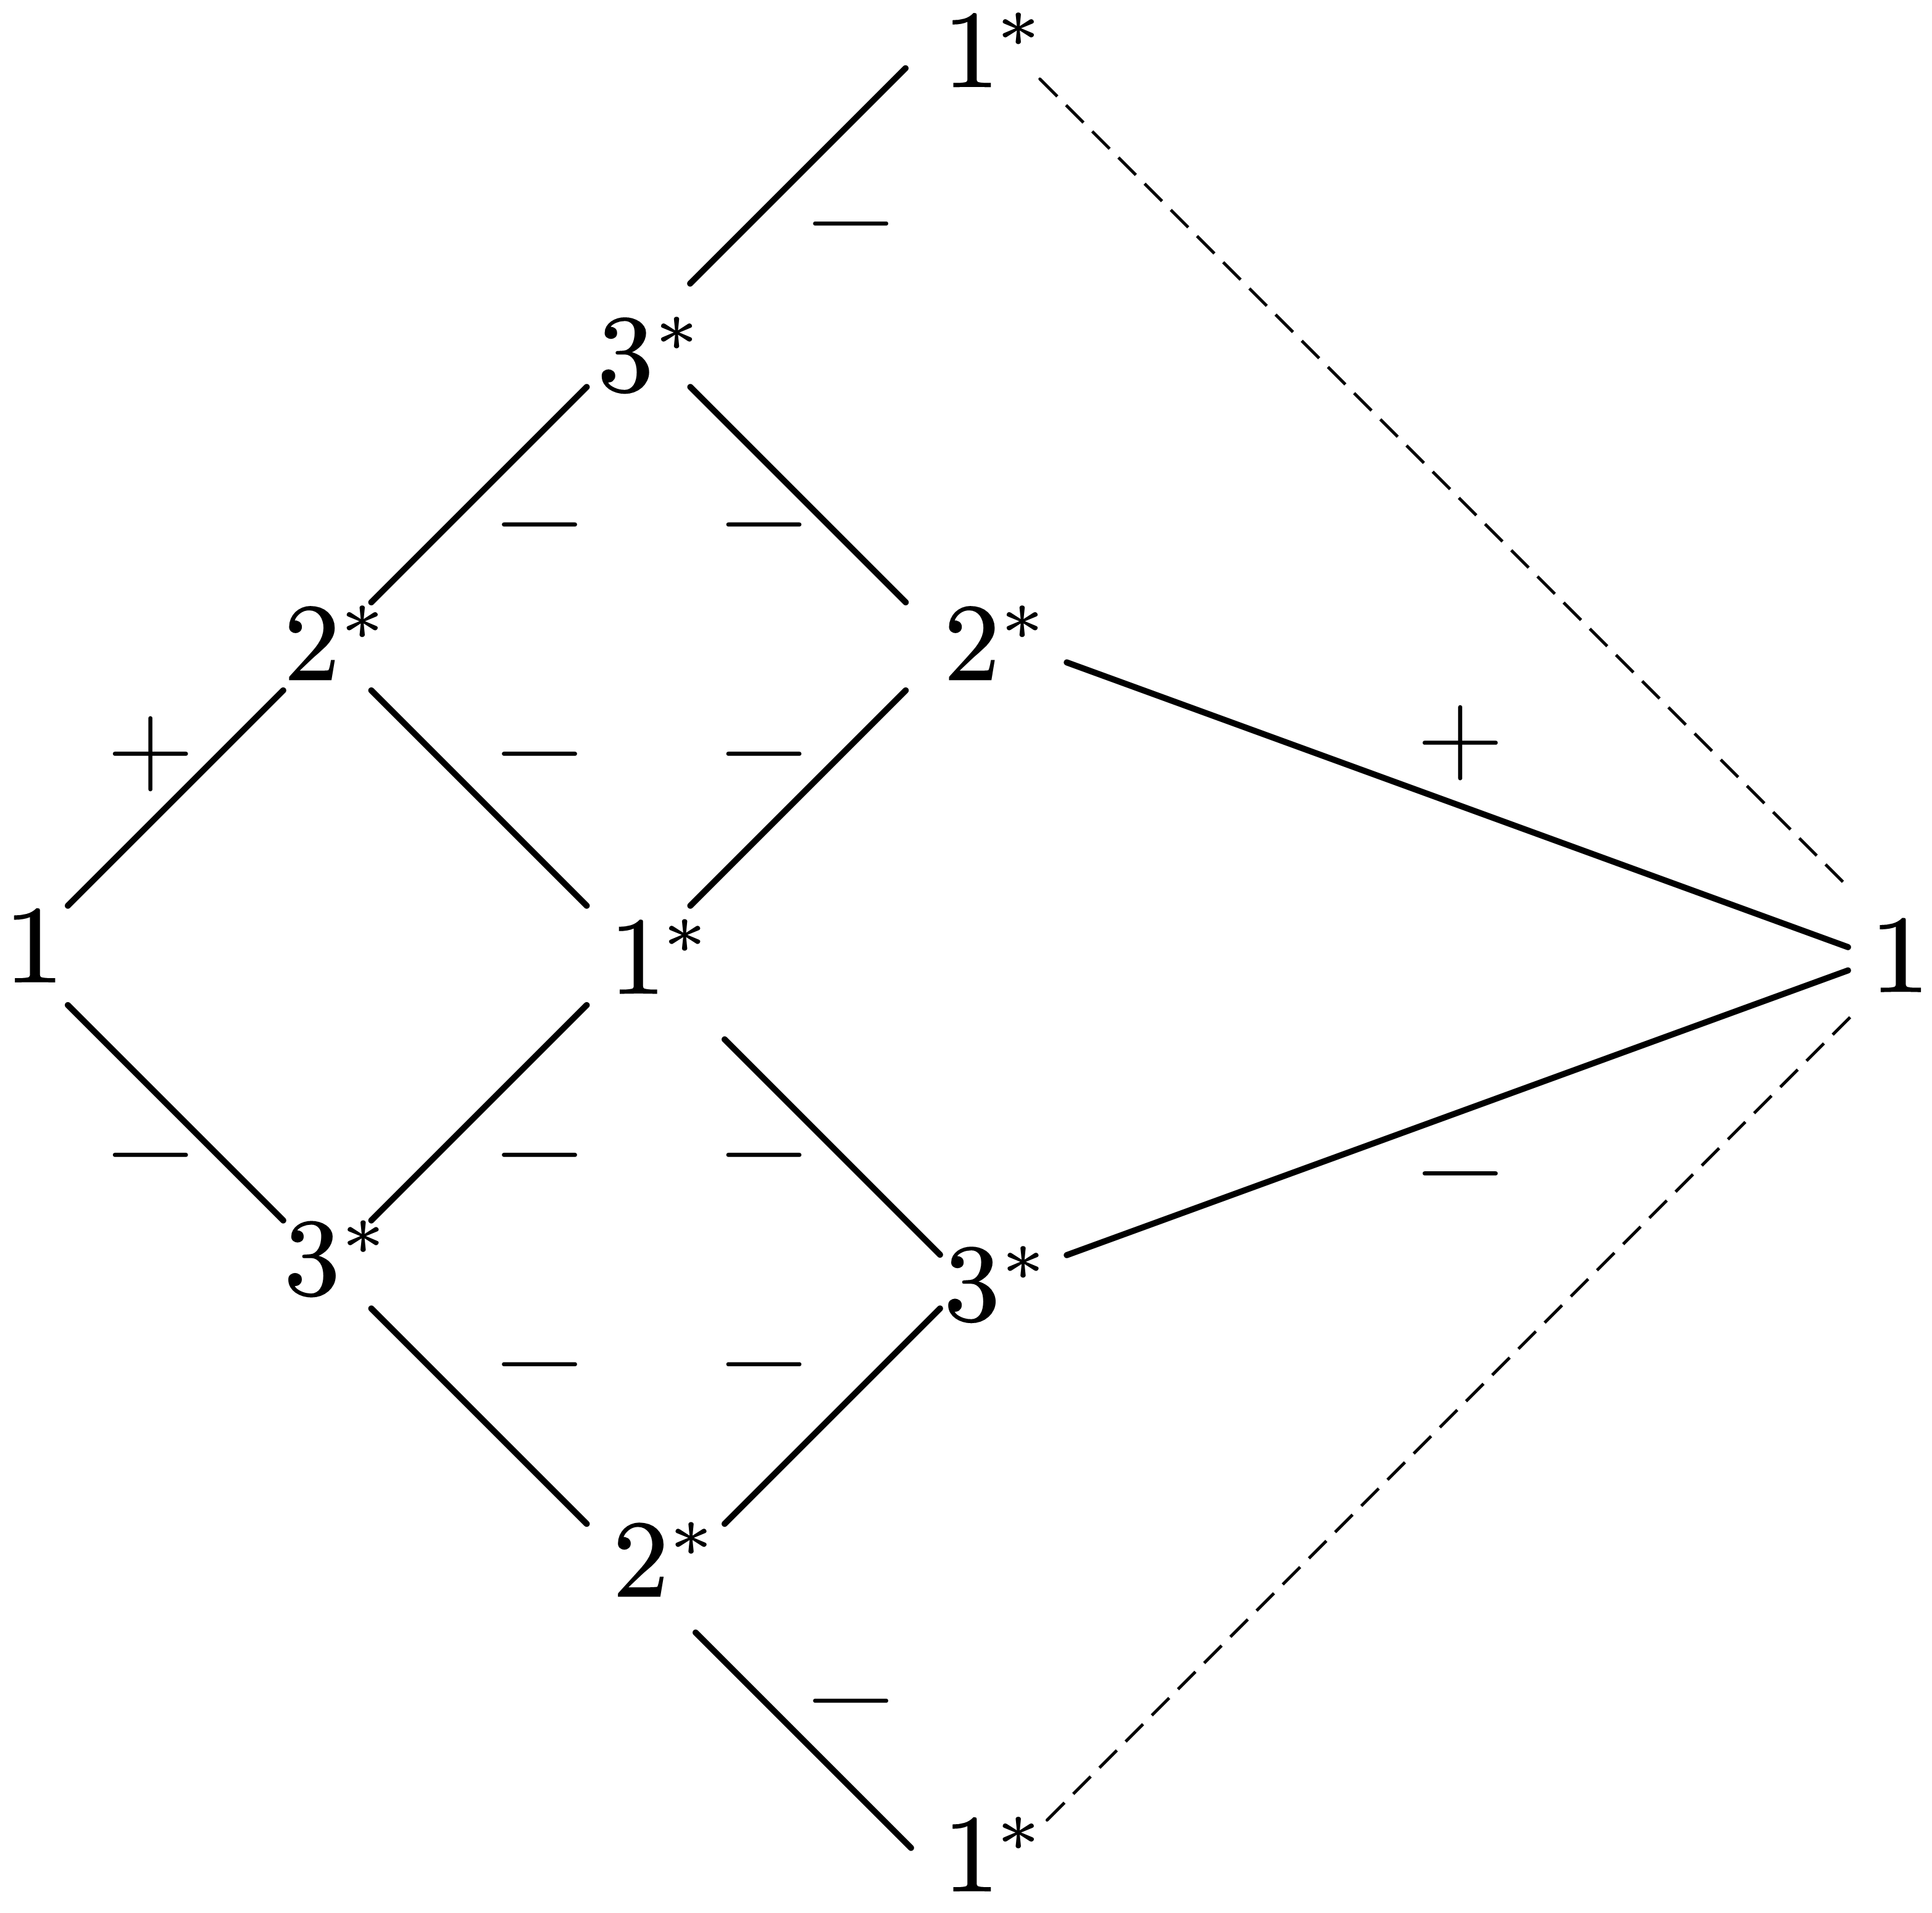
\includegraphics[scale=0.5,trim=0 -8 0 -8]{./pictures/6.07/pictorial_representation_3.png}
		\end{minipage} \\
		
		\begin{minipage}{0.3\linewidth}
		\centering
		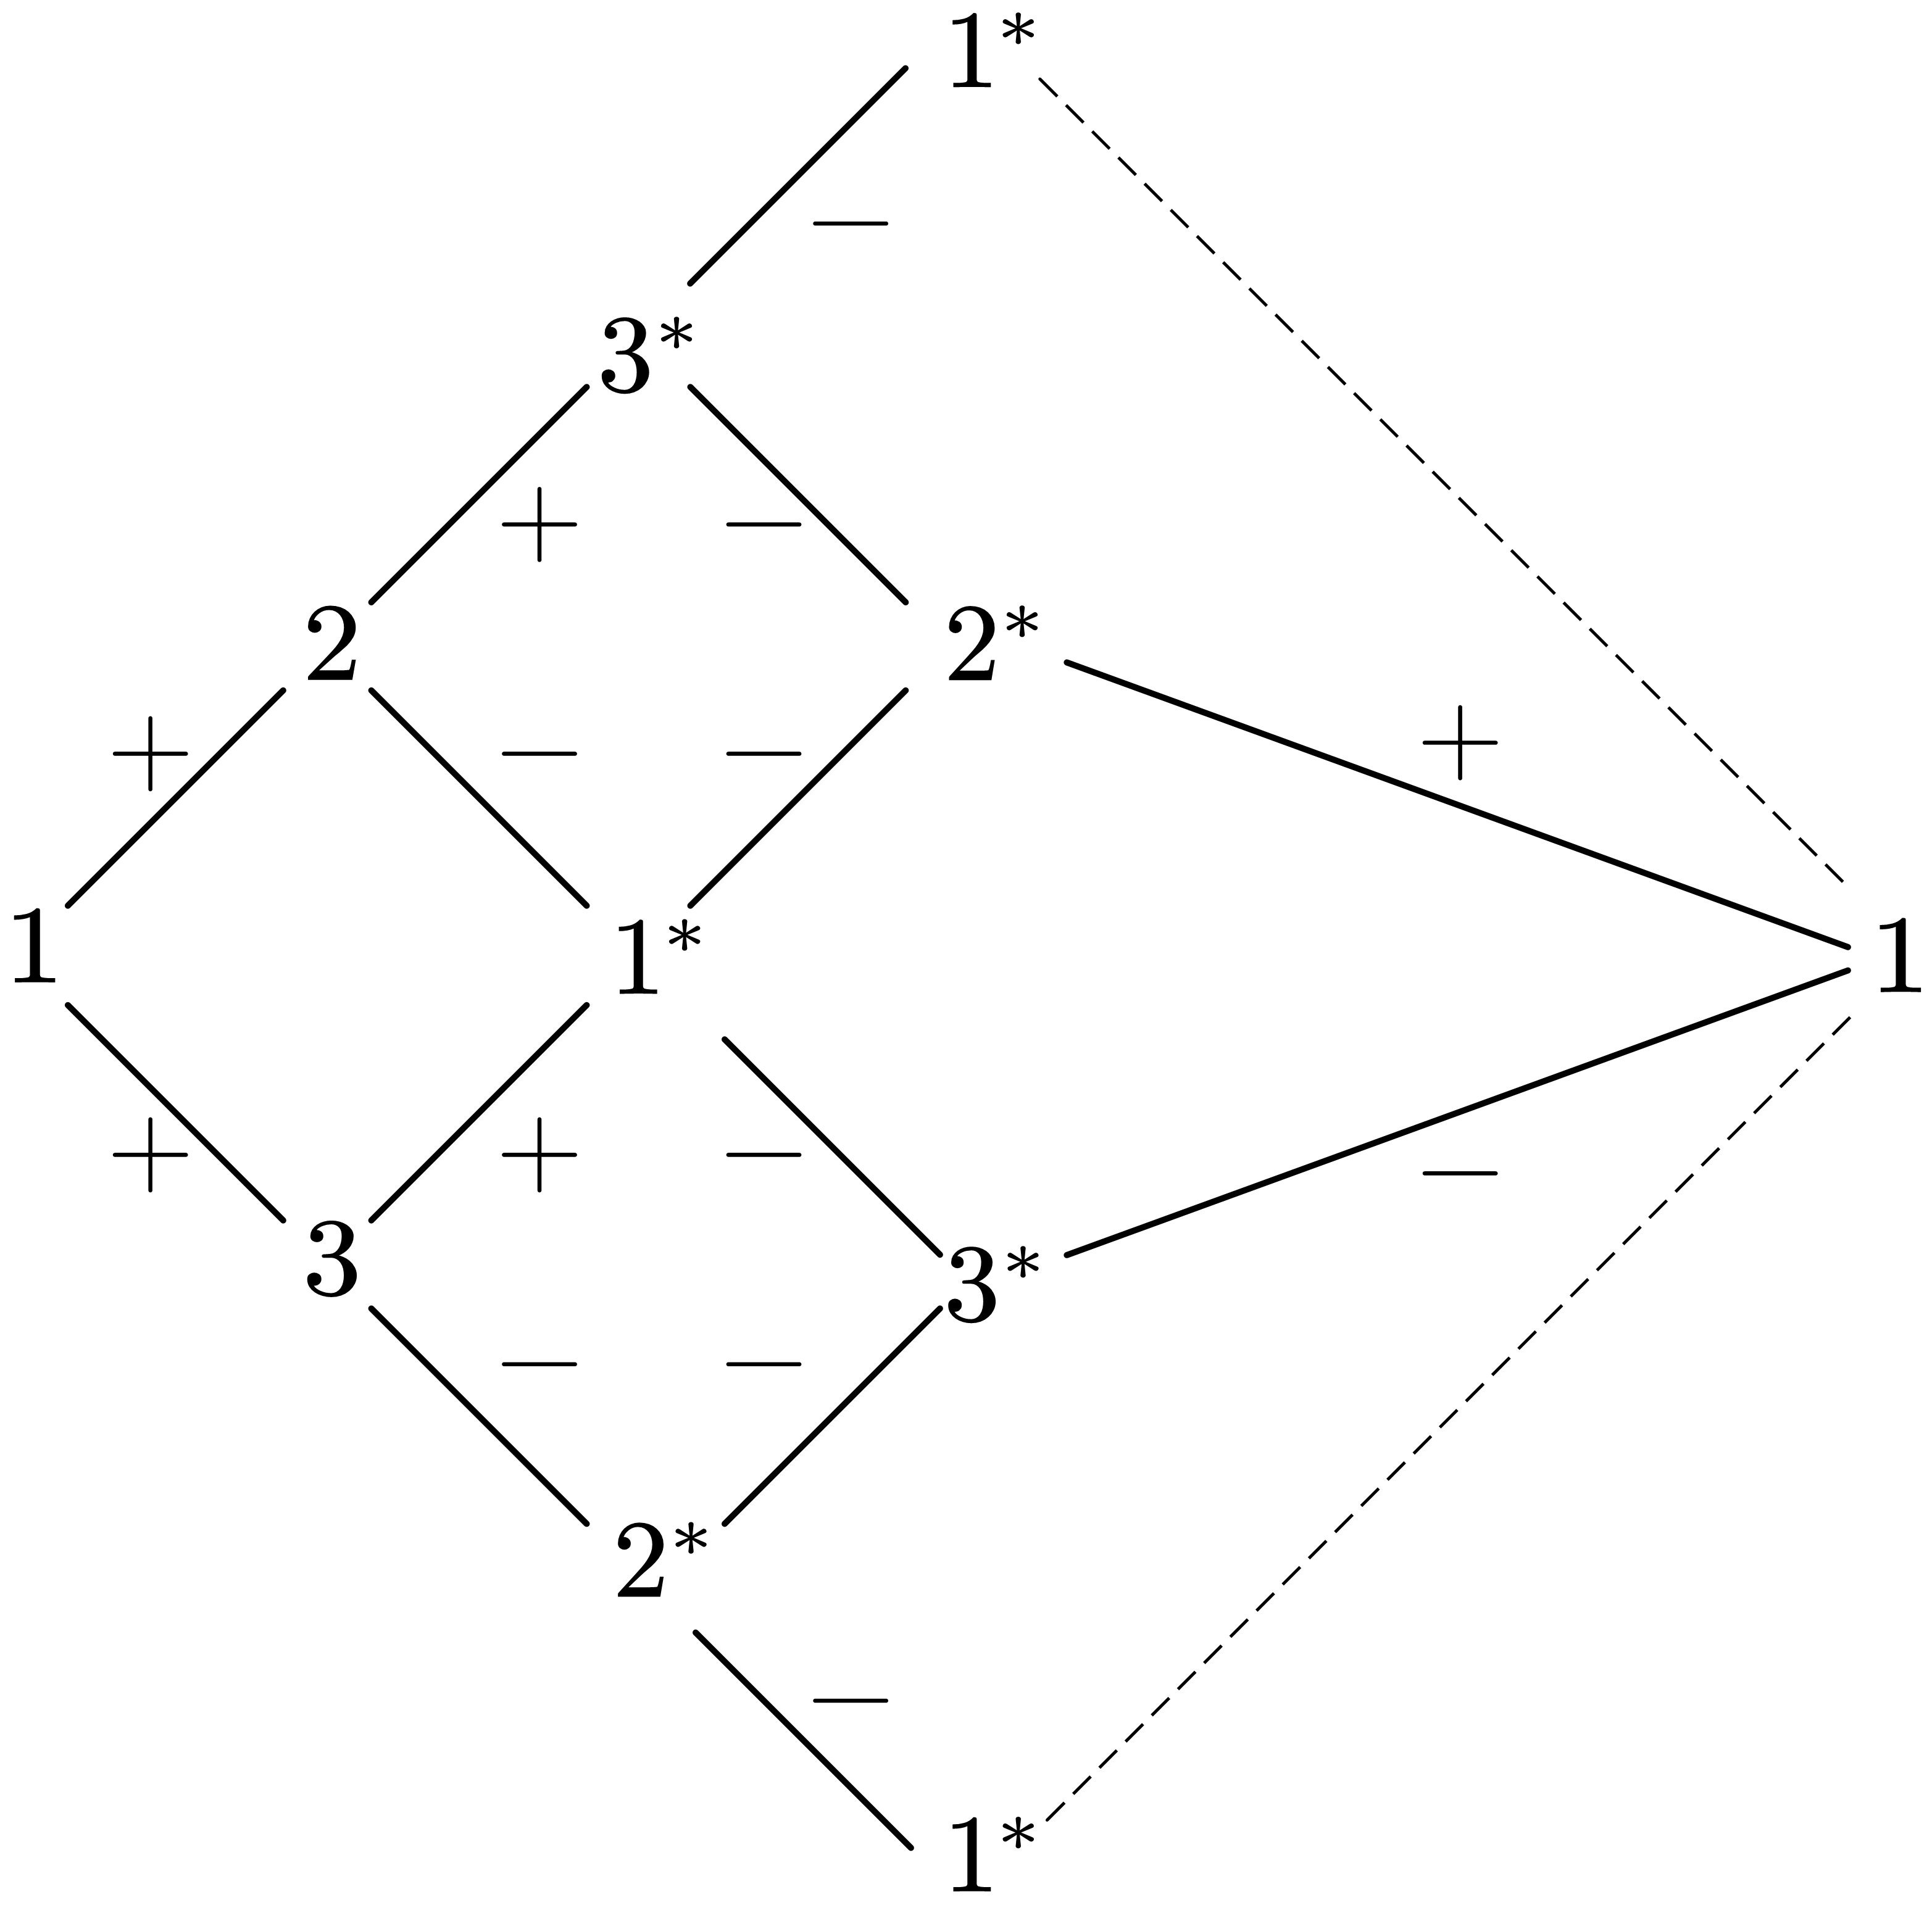
\includegraphics[scale=0.5,trim=0 -8 0 -8]{./pictures/6.07/pictorial_representation_4.png}
		\end{minipage} &
			
		\begin{minipage}{0.3\linewidth}
		\centering
		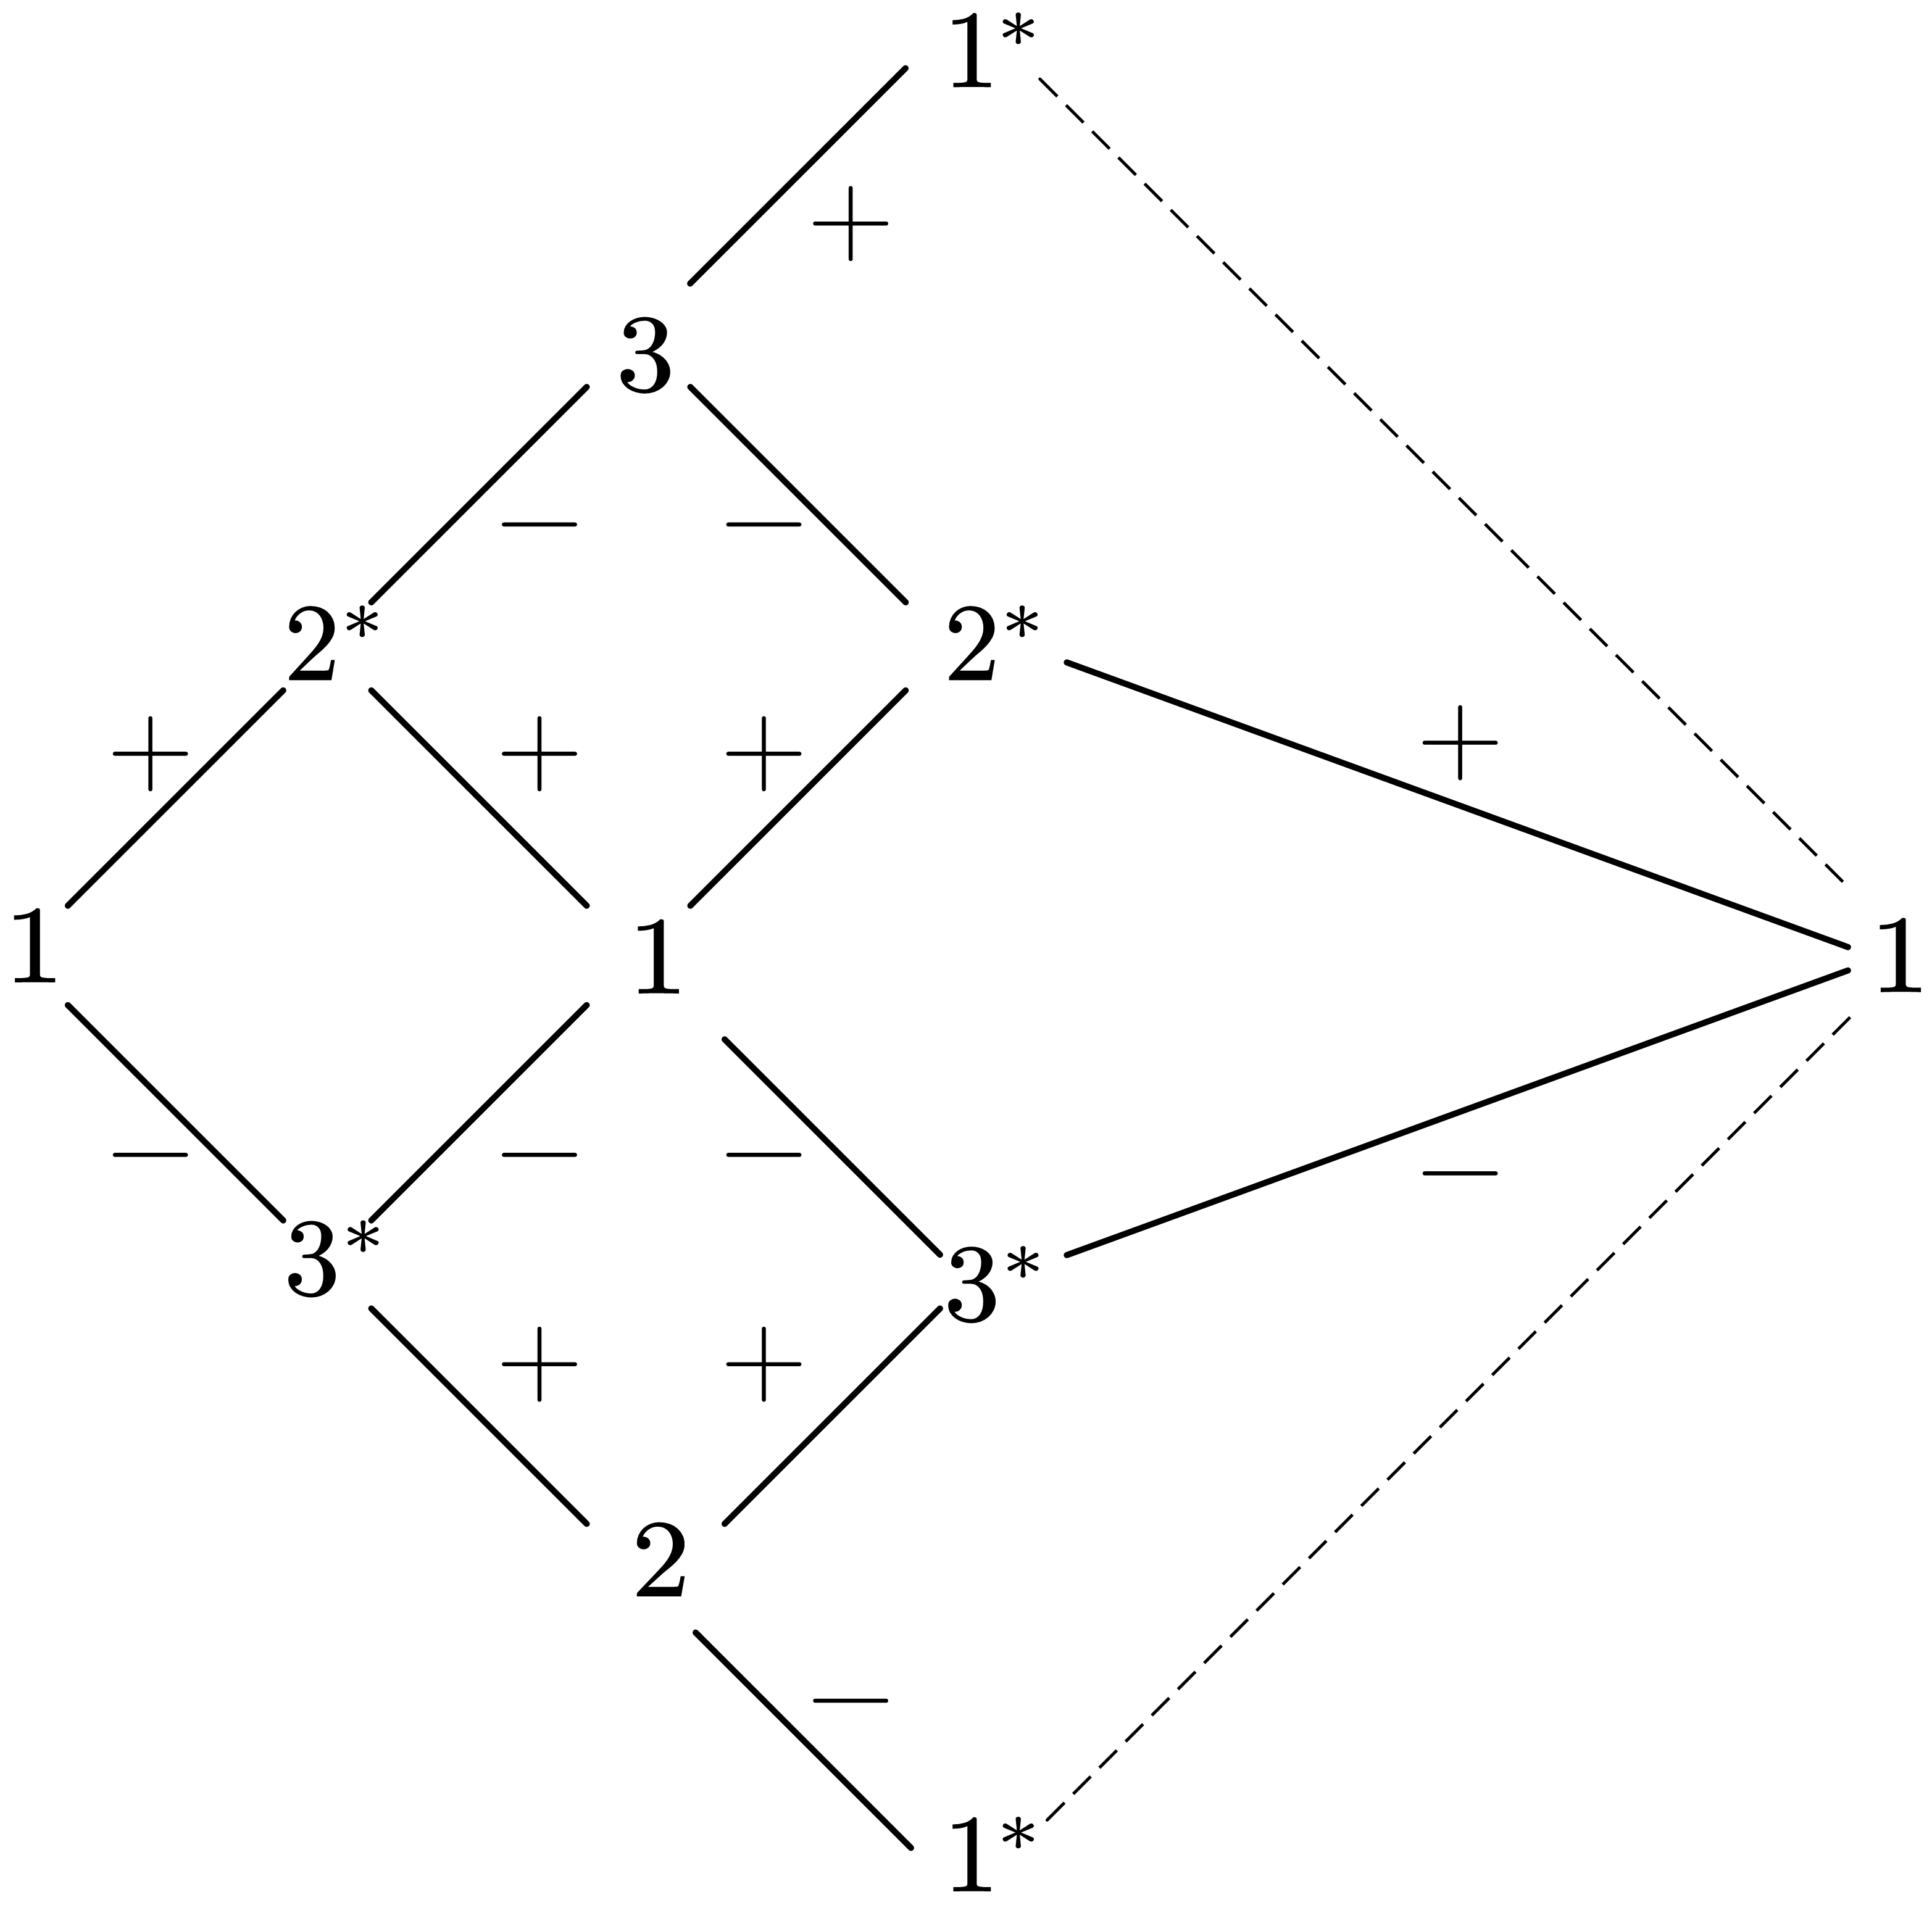
\includegraphics[scale=0.5,trim=0 -8 0 -8]{./pictures/6.07/pictorial_representation_5.png}
		\end{minipage} &
		
		\begin{minipage}{0.3\linewidth}
		\centering
		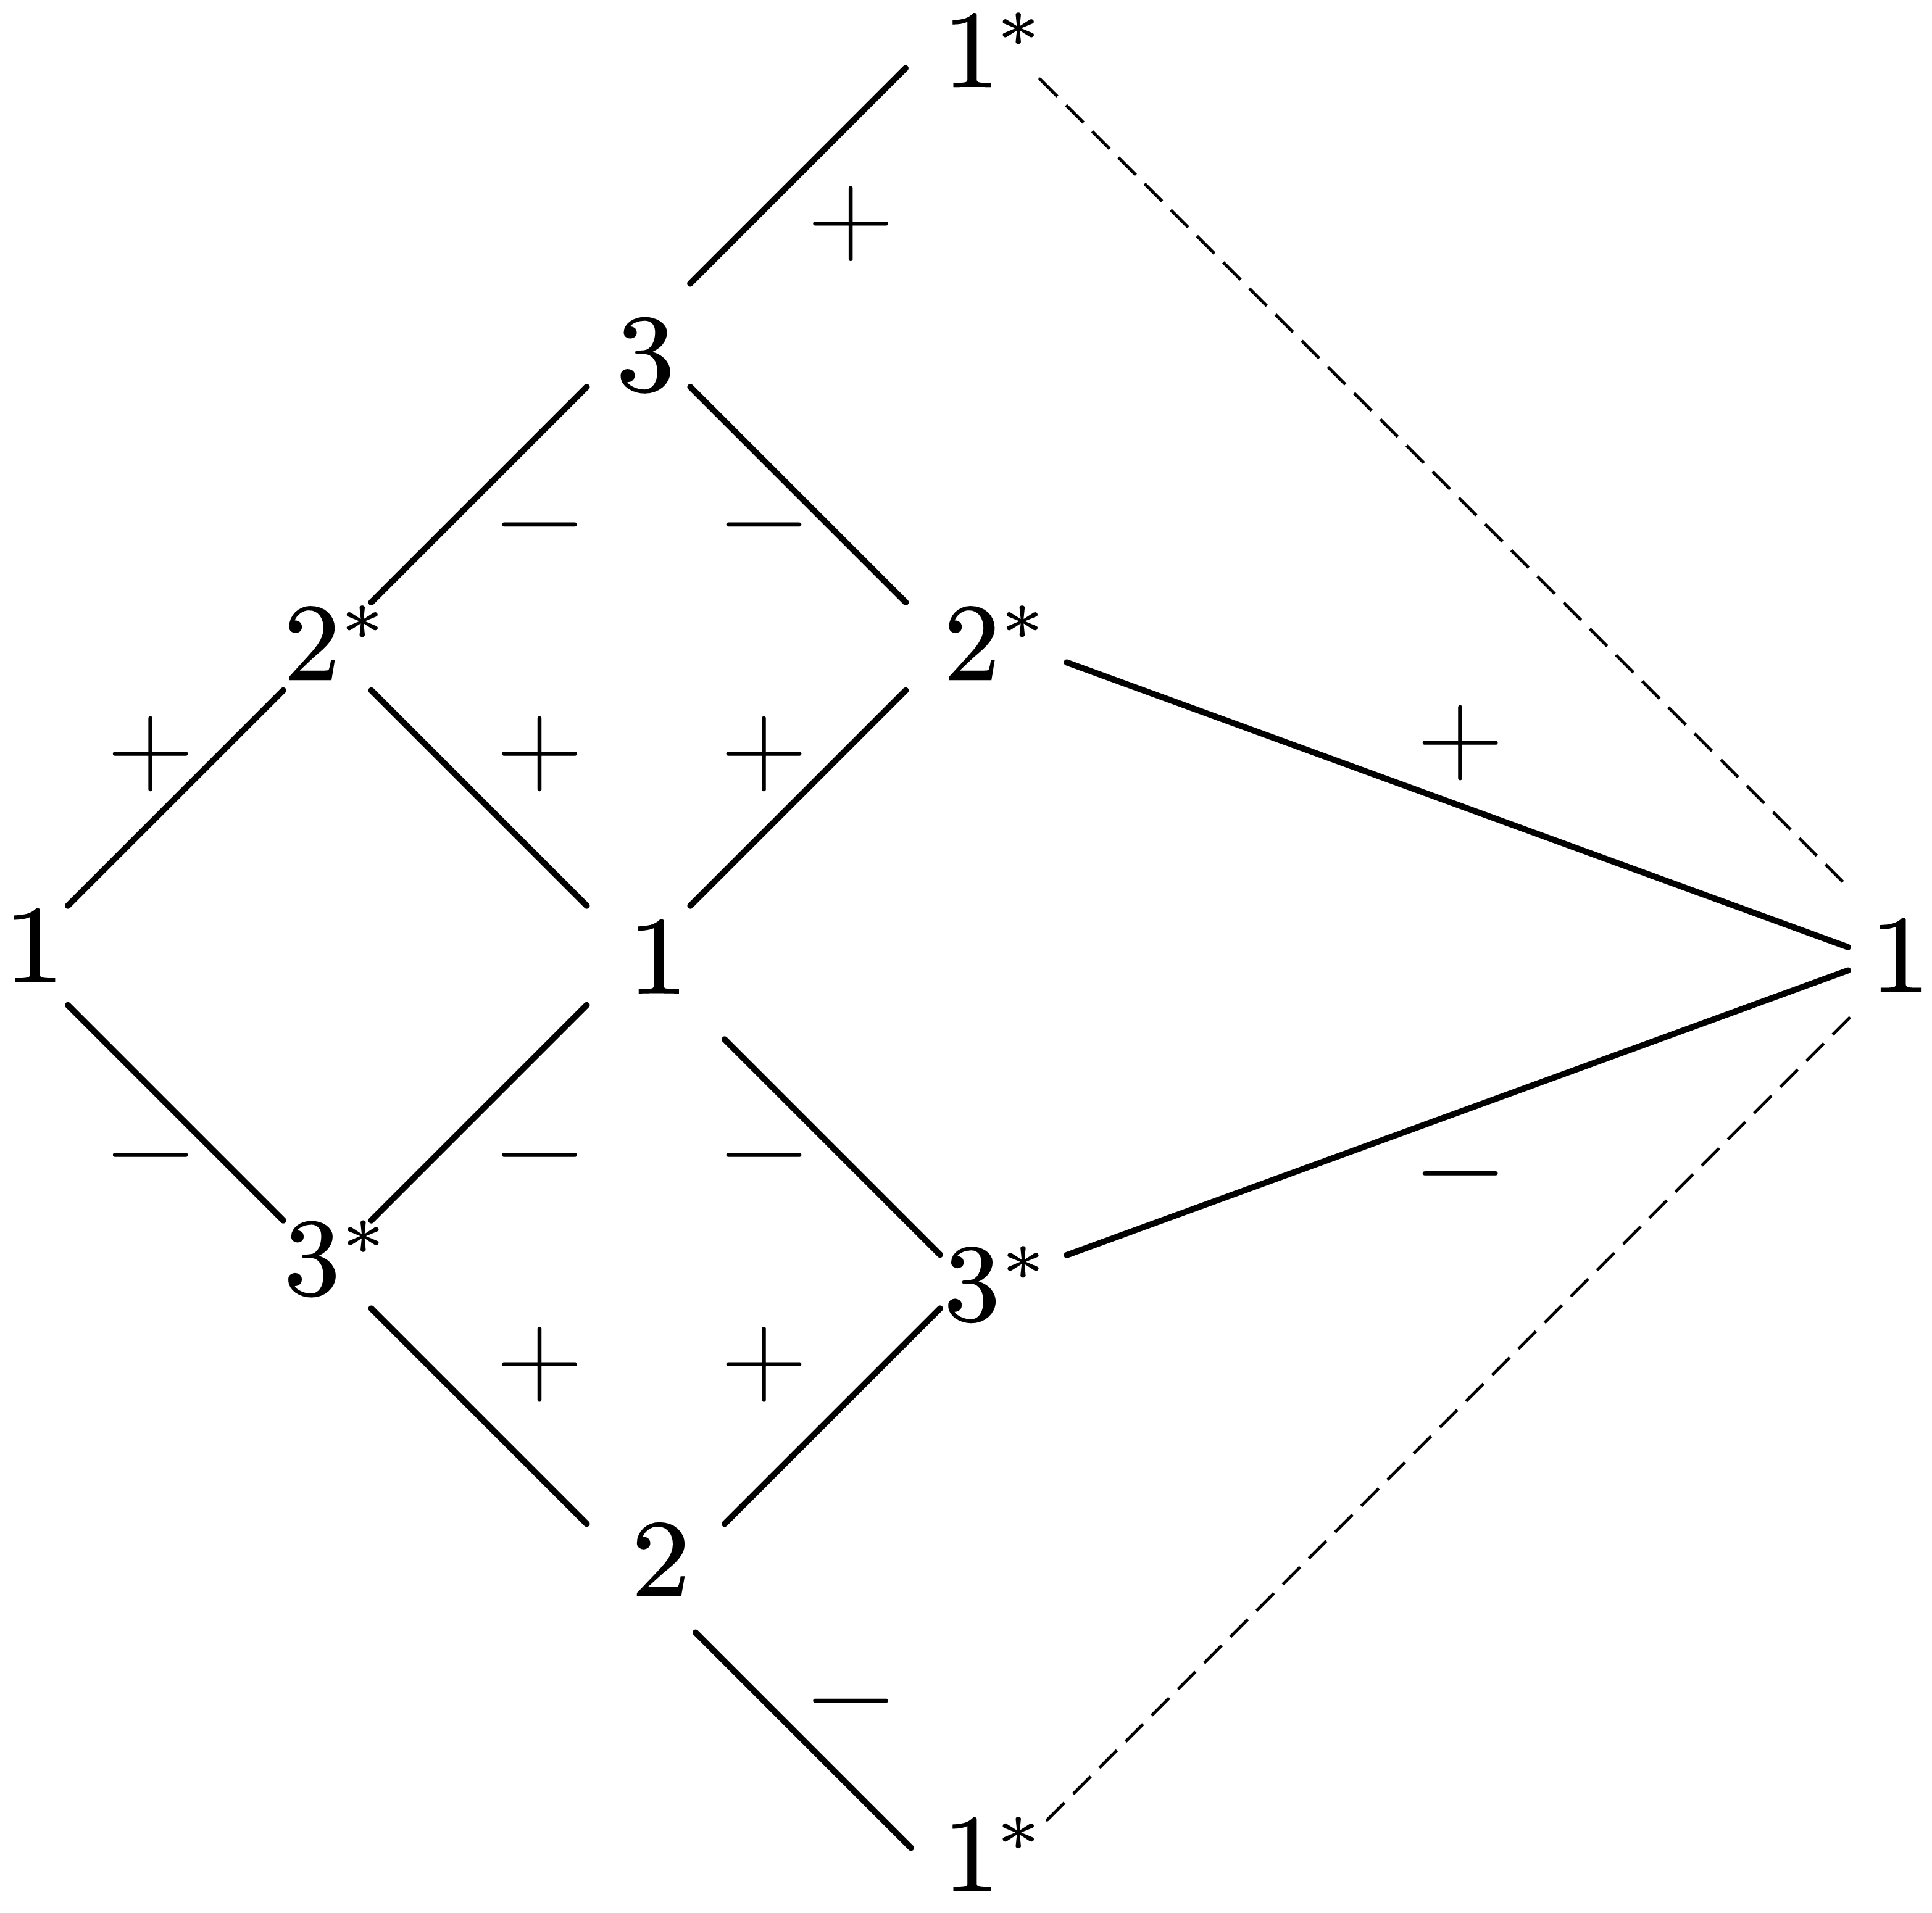
\includegraphics[scale=0.5,trim=0 -8 0 -8]{./pictures/6.07/pictorial_representation_6.png}
		\end{minipage}
		
	\end{tabular}
	\captionof{figure}{The pictorial representation of all fourth-order diagrams of the benzene.}\label{fig:exe7_2}
	\end{center}
	
	Now we will calculate all terms according to their pictorial representation. Instead of lengthy calculation, we only care about the path from 1 to 1 in each diagram. For example, for the first subdiagram of \Figref{fig:exe7_2}, we know that it has eight paths, six valid but two invalid. If a path has a segment with a plus/minus token, it will be marked as $+$/$-$, and zero otherwise. And thus, its eight paths are:
	\begin{center}
	\begin{tabular}{cccc}
		$(+,+,-,0)$ & $(+,+,-,+)$ & $(+,-,-,+)$ & $(+,-,-,-)$\\
		$(+,+,-,+)$ & $(+,+,-,-)$ & $(+,-,-,-)$ & $(+,-,-,0)$
	\end{tabular}
	\end{center}		
	If a path has a 0, the corresponding term is zero. Otherwise, the corresponding term has a factor $(-1)^k$, where $k$ is the number of its minus signs. Therefore, there are two positive and four negative terms, and the first term is
	\[
		(-1)^{2+1} \frac{2 \times 3}{ (2\beta)^3 } \left[ 2 \times \left( \frac{\beta^4}{16} \right) + 4 \times \left( -\frac{\beta^4}{16} \right) \right] = \frac{6}{64} \beta = \frac{N}{64} \beta,
	\]
	where the factor $2$ occurs for the closed-shell structure, and the factor $3$ is the number of occupied spin orbitals.
	
	Similarly, we find that the second, third, ..., sixth term is $\frac{N}{64} \beta$, $\frac{N}{64} \beta$, $\frac{N}{64} \beta$, $-\frac{3N}{128} \beta$, $-\frac{3N}{128} \beta$. Thus, we obtain that
	\begin{sequation}
		E^{(4)}_0 = 4 \times \left( \frac{N}{64} \beta \right) + 2 \times \left( -\frac{3N}{128} \beta \right) = \frac{N}{64} \beta.
	\end{sequation}

	\item[b.] As mentioned before, the general expression of the correlation energy with $N>6$ is also suitable for benzene. Thus, the correlation energy of the benzene is
	\begin{sequation}
		E^{(4)}_0({\rm benzene} ) = \frac{6}{64} \beta = \frac{3}{32} \beta,
	\end{sequation}		
	which agrees with the independently calculated result found in Exercise 6.6.
	
	\end{itemize}	
	
	\end{solution}
	
	\section{Perturbation Expansion of the Correlation Energy}
	
	% 6.8
	\begin{exercise}
	Derive Eqs.(6.73) and (6.74) starting with Eq.(6.72).
	\end{exercise}
	
	\begin{solution}

	The detailed simplification can be seen in Exercise 2.18.
	
	\end{solution}
	
	% 6.9
	\begin{exercise}
	Derive Eqs.(6.77) and (6.78) from Eq.(6.76).
	\end{exercise}
	
	\begin{solution}
	We assume that $\Delta \approx (\varepsilon_2 - \varepsilon_1)$, thus	
	\[
		\Delta = ( \varepsilon_2 - \varepsilon_1 ) + \frac{1}{2} J_{11} + \frac{1}{2} J_{22} - 2 J_{12} + K_{12} = ( \varepsilon_2 - \varepsilon_1 ) \left[ 1 + \frac{ J_{11} + J_{22} - 4 J_{12} + 2 K_{12} }{ 2 ( \varepsilon_2 - \varepsilon_1 ) } \right].
	\]
	Using binomial series and geometric series, we find that
	\begin{align*}
		E_\corr &= \Delta - \left( \Delta^2 + K^2_{12} \right)^{\frac{1}{2}} = \Delta \left[ 1 - \left( 1 + \frac{ K^2_{12} }{ \Delta^2 } \right)^{\frac{1}{2}} \right] = \Delta \left[ 1 - \left( 1 + \frac{ K^2_{12} }{ 2\Delta^2 } - \frac{ K^4_{12} }{ 8\Delta^4 } + \cdots \right) \right] \\
		&= - \frac{ K^2_{12} }{ 2\Delta } + \frac{ K^4_{12} }{ 8\Delta^3 } + \cdots \\
		&= - \frac{ K^2_{12} }{ 2( \varepsilon_2 - \varepsilon_1 ) \left[ 1 + \frac{ J_{11} + J_{22} - 4 J_{12} + 2 K_{12} }{ 2 ( \varepsilon_2 - \varepsilon_1 ) } \right] } + \frac{ K^4_{12} }{ 8 ( \varepsilon_2 - \varepsilon_1 )^3 \left[ 1 + \frac{ J_{11} + J_{22} - 4 J_{12} + 2 K_{12} }{ 2 ( \varepsilon_2 - \varepsilon_1 ) } \right]^3 } + \cdots \\
		&= - \frac{ K^2_{12} }{ 2( \varepsilon_2 - \varepsilon_1 )} \left[ 1 - \frac{ J_{11} + J_{22} - 4 J_{12} + 2 K_{12} }{ 2 ( \varepsilon_2 - \varepsilon_1 ) } + \left( \frac{ J_{11} + J_{22} - 4 J_{12} + 2 K_{12} }{ 2 ( \varepsilon_2 - \varepsilon_1 ) } \right)^2 + \cdots \right] + \cdots \\
		&= - \frac{ K^2_{12} }{ 2( \varepsilon_2 - \varepsilon_1 )} + \frac{ K^2_{12} ( J_{11} + J_{22} - 4 J_{12} + 2 K_{12} ) }{ 4( \varepsilon_2 - \varepsilon_1 )^2 } + o\left( \left( \frac{1}{ \varepsilon_2 - \varepsilon_1 } \right)^2 \right) .
	\end{align*}
	Thus, we obtain (6.77) and (6.78) from (6.76).
	
	\end{solution}
	
	\section{The \texorpdfstring{$N$}--Dependence of the RS Perturbation Expansion}
	
	% 6.10
	\begin{exercise}
	Derive Eqs.(6.80b) and (6.90).
	\end{exercise}
	
	\begin{solution}
	From (6.68), we find that with the truth that all two-electron integrals involving orbitals from different units are zero and $\langle mm || mm \rangle = 0$,
	\begin{align*}
		E^{(1)}_0 &= - \frac{1}{2} \sum_{ i=1 }^{2N} \sum_{ j=1 }^{2N} \langle 1_i 1_j || 1_i 1_j \rangle = - \frac{1}{2} \sum_{ i=1 }^{2N} \langle 1_i 1_i || 1_i 1_i \rangle \\
			&= - \frac{1}{2} \sum_{ i=1 }^N \langle 1_i 1_i || 1_i 1_i \rangle + \langle 1_i \bar{1}_i || 1_i \bar{1}_i \rangle + \langle \bar{1}_i 1_i || \bar{1}_i 1_i \rangle + \langle \bar{1}_i \bar{1}_i || \bar{1}_i \bar{1}_i \rangle = -\frac{1}{2} \sum_{ i=1 }^N 2J_{11} = -\sum_{ i=1 }^N J_{11} = -N J_{11}.
	\end{align*}
	
	Besides, we obtain that
	\begin{align*}
		\langle \Psi^{2_i \bar{2}_i}_{1_i \bar{1}_i} | \mathscr{V} | \Psi^{2_i \bar{2}_i}_{1_i \bar{1}_i} \rangle &= \langle \Psi^{2_i \bar{2}_i}_{1_i \bar{1}_i} | \mathscr{H} | \Psi^{2_i \bar{2}_i}_{1_i \bar{1}_i} \rangle - \langle \Psi^{2_i \bar{2}_i}_{1_i \bar{1}_i} | \mathscr{H}_0 | \Psi^{2_i \bar{2}_i}_{1_i \bar{1}_i} \rangle \\
		&= \sum_{ i=1 }^{2N} h_{11} + 2h_{22} - 2h_{11} + \sum_{ i=1 }^N  J_{11} + J_{22} - J_{11} - \left[ ( 2N - 2 ) \varepsilon_1 + 2\varepsilon_2 \right] \\
		&= (2N-2)h_{11} + 2h_{22} + (N-1) J_{11} + J_{22} - (2N-2) ( h_{11} + J_{11} ) - 2 (h_{22} + 2J_{12} - K_{12})\\
		&= -(N-1) J_{11} + J_{22} - 4J_{12} + 2K_{12}. 
	\end{align*}
	
	\end{solution}
	
	\sectionstar{Diagrammatic Representation of the Perturbation Expansion of the Correlation Energy}
	
	\subsection{Hugenholtz Diagrams}
	
	% 6.11
	\begin{exercise}
	Show that the fourth-order diagram
	
	\begin{center}
	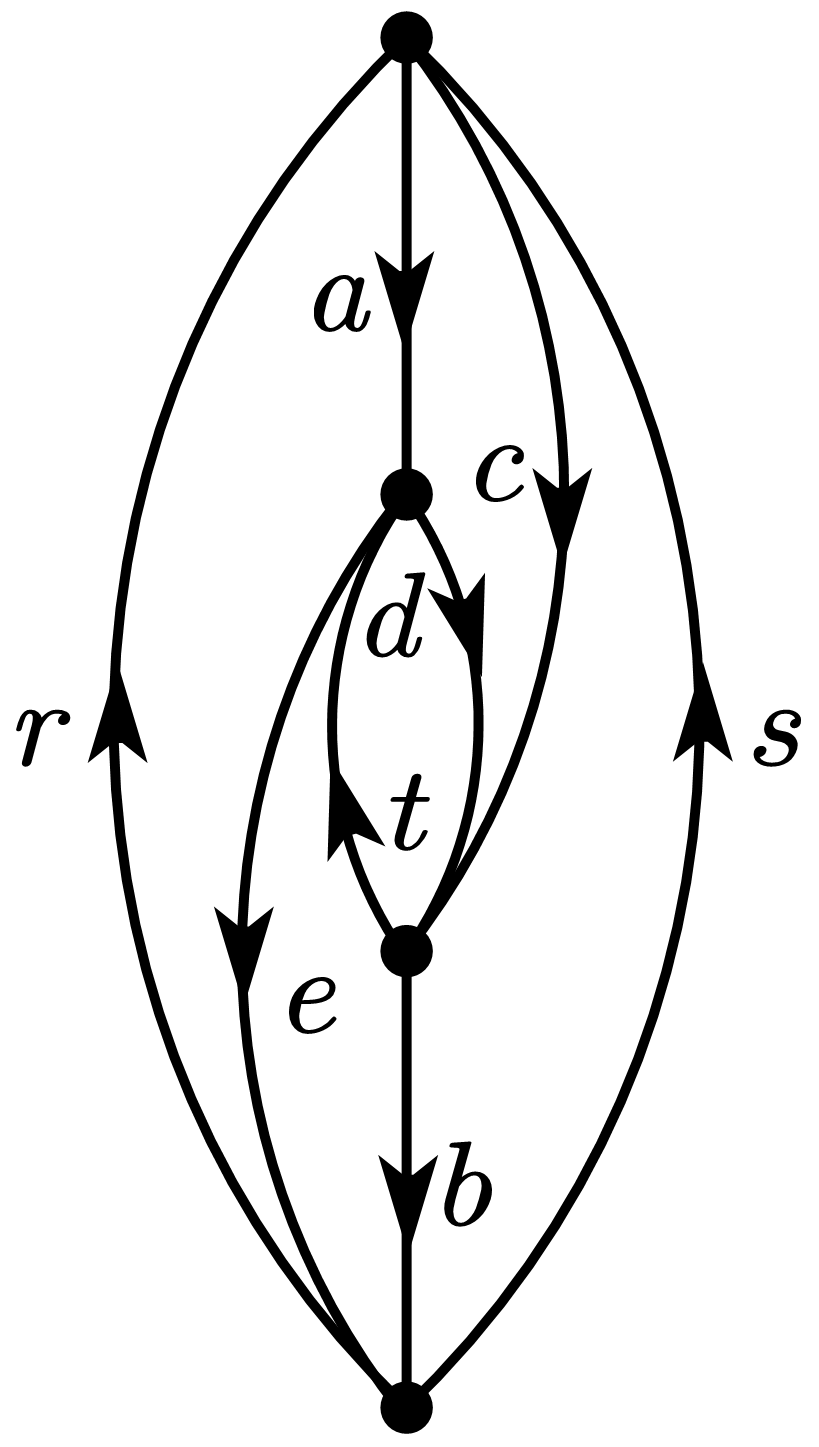
\includegraphics[scale=0.9]{./pictures/6.11/exercise.png}
	\end{center}
	is equal to
	\[
		-\frac{1}{2} \sum_{abcderst} \frac{ \langle rs || ac \rangle \langle at || de \rangle \langle dc || tb \rangle \langle eb||rs \rangle }{ ( \varepsilon_a + \varepsilon_c - \varepsilon_r - \varepsilon_s ) ( \varepsilon_c + \varepsilon_d + \varepsilon_e - \varepsilon_r - \varepsilon_t - \varepsilon_s ) ( \varepsilon_b + \varepsilon_e - \varepsilon_r - \varepsilon_s ) }.
	\]	
	
	\end{exercise}
	
	\begin{solution}
	
	Using the diagrammatic method, this term is made of four parts as follows.
	\begin{enumerate}
	
	\item There are 5 hole lines ($a$, $b$, $c$, $d$, $e$) and 3 particle lines ($r$, $s$, $t$). Thus we add a summation token with subscripts $abcderst$. 
	
	\item There are 2 loops, $r \rightarrow a \rightarrow d \rightarrow t \rightarrow e \rightarrow r$, $s \rightarrow c \rightarrow b \rightarrow s$, and 5 hole lines, thus we should add a $(-1)^{2+5} = (-1)^7$.	
	
	\item From the top to the bottom, 4 dots contribute $\langle rs|| ac \rangle$, $\langle at||de \rangle$, $\langle dc || tb \rangle$, $\langle eb || rs \rangle$, respectively.
	
	\item There are 3 imaginary horizontal lines.
		\begin{itemize}
		
		\item The first one crosses $a$, $c$, $r$, $s$, contributing a factor $\varepsilon_a + \varepsilon_c - \varepsilon_r - \varepsilon_s$ to the denominator.
		
		\item The second one crosses $c$, $d$, $e$, $r$, $t$, $s$ contributing a factor $\varepsilon_c + \varepsilon_d + \varepsilon_e - \varepsilon_r - \varepsilon_t - \varepsilon_s$ to the denominator.
		
		\item The third one crosses $b$, $e$, $r$, $s$, contributing a factor $\varepsilon_b + \varepsilon_e - \varepsilon_r - \varepsilon_s$ to the denominator.
		
		\end{itemize}			
	
	\end{enumerate}
	
	In conclusion, we know the mathematical expression of this diagram is
	\begin{sequation}
		-\frac{1}{2} \sum_{abcderst} \frac{ \langle rs || ac \rangle \langle at || de \rangle \langle dc || tb \rangle \langle eb||rs \rangle }{ ( \varepsilon_a + \varepsilon_c - \varepsilon_r - \varepsilon_s ) ( \varepsilon_c + \varepsilon_d + \varepsilon_e - \varepsilon_r - \varepsilon_t - \varepsilon_s ) ( \varepsilon_b + \varepsilon_e - \varepsilon_r - \varepsilon_s ) }.
	\end{sequation}
	
	\end{solution}
	
	\subsection{Goldstone Diagrams}
	
	% 6.12
	\begin{exercise}
	We stated that the Goldstone diagrams in Table 6.2 can be obtained by ``pulling apart" the second- and third-order Hugenholtz diagrams. This is quite tricky to see but the converse is much easier. For example, if we push
	
	\begin{center}
	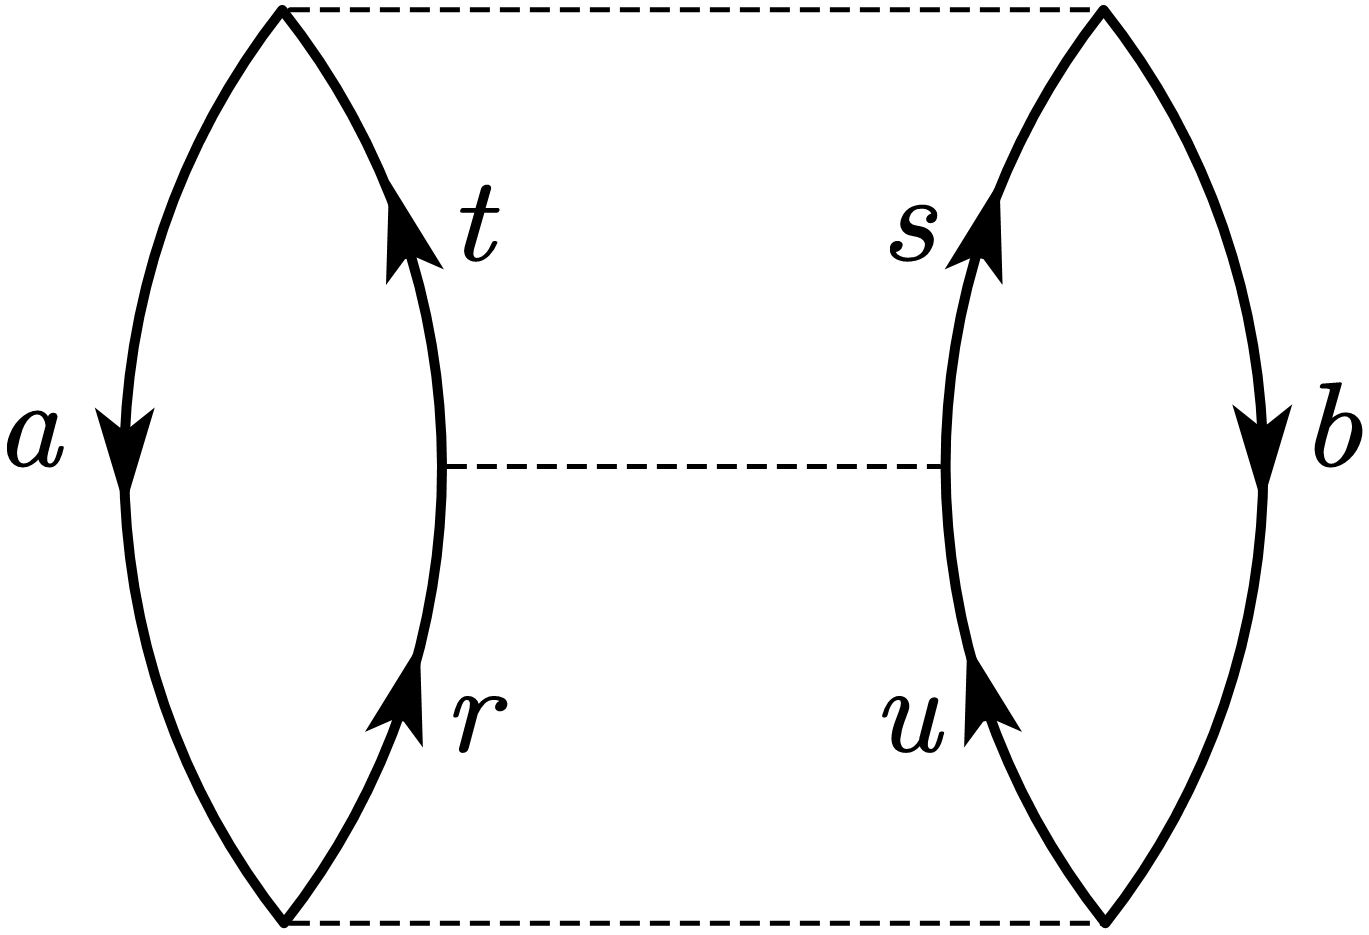
\includegraphics[scale=0.9]{./pictures/6.12/exercise_1.png}
	\end{center}
	
	together, it is clear that we obtain
	
	\begin{center}
	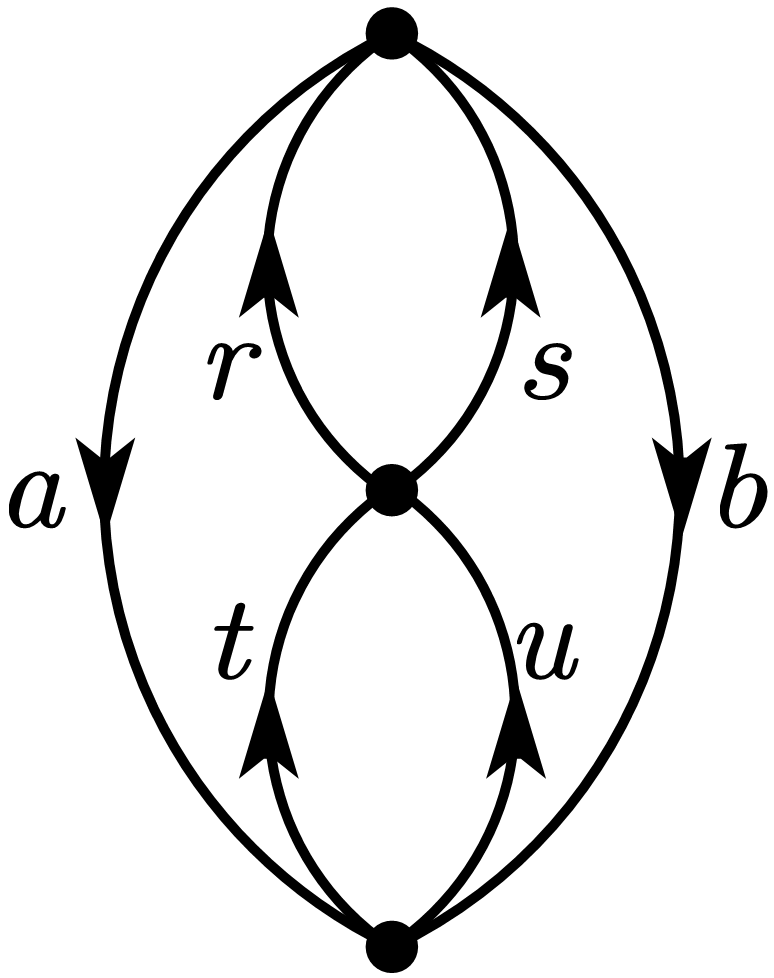
\includegraphics[scale=0.9]{./pictures/6.12/exercise_2.png}
	\end{center}
	
	Push all third-order diagrams in Table 6.2 together in a similar way and, thus, find which Goldstone diagram comes from which Hugenholtz diagram. For the above Hugenholtz diagram, verify that its mathematical value is indeed the sum of the values of the corresponding Goldstone diagrams.
	
	\end{exercise}
	
	\begin{solution}

	As the textbook mentioned at the page 361, there are three third-order Hugenholtz diagrams, which are listed in \Figref{fig:exe12_1}.

	\begin{center}
	\begin{tabular}{ccc}
	
		\begin{minipage}{0.22\linewidth}
		\centering
		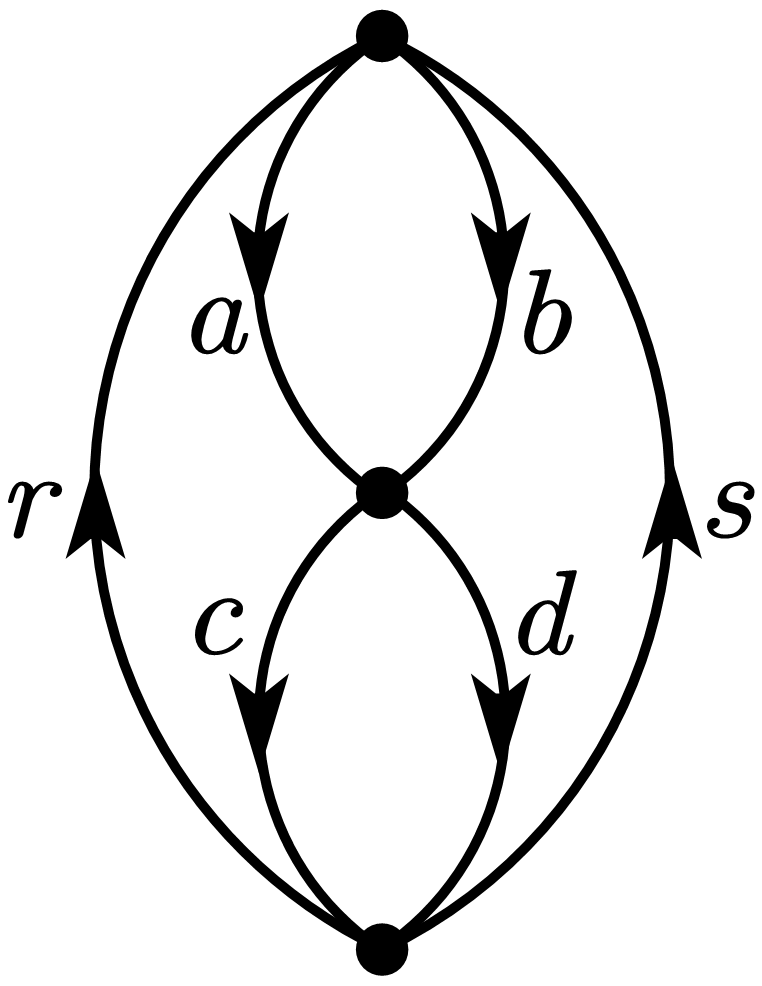
\includegraphics[scale=1.0,trim=0 -4 0 -4]{./pictures/6.12/hugenholtz_1.png}
		\end{minipage} &
		
		\begin{minipage}{0.22\linewidth}
		\centering
		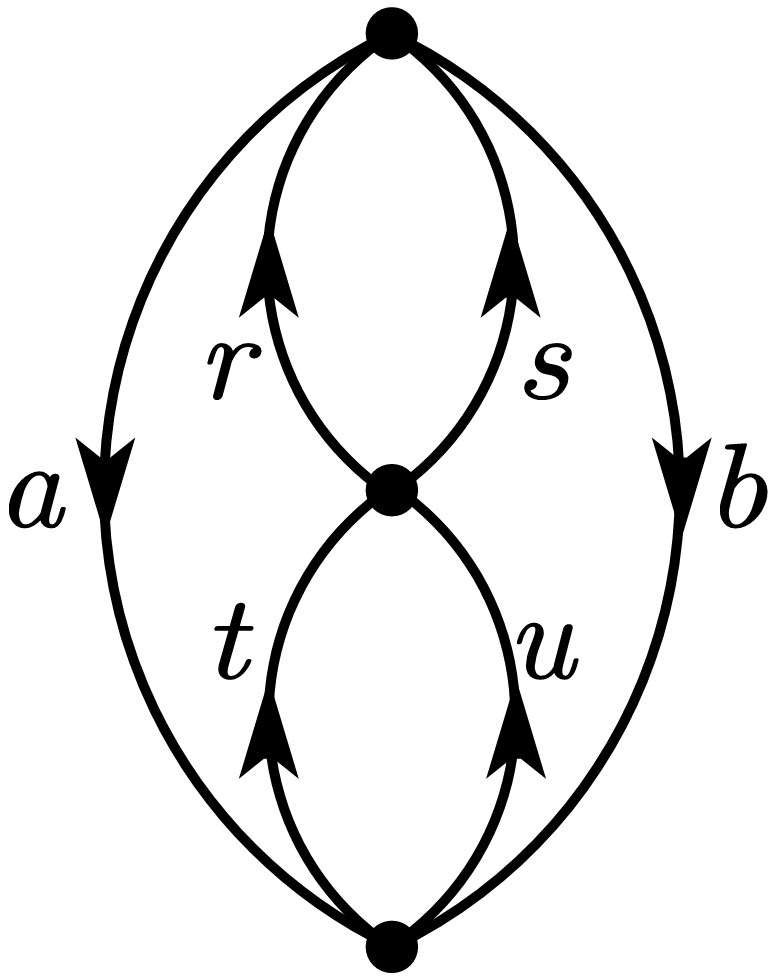
\includegraphics[scale=1.0,trim=0 -4 0 -4]{./pictures/6.12/hugenholtz_2.png}
		\end{minipage} &
		
		\begin{minipage}{0.22\linewidth}
		\centering
		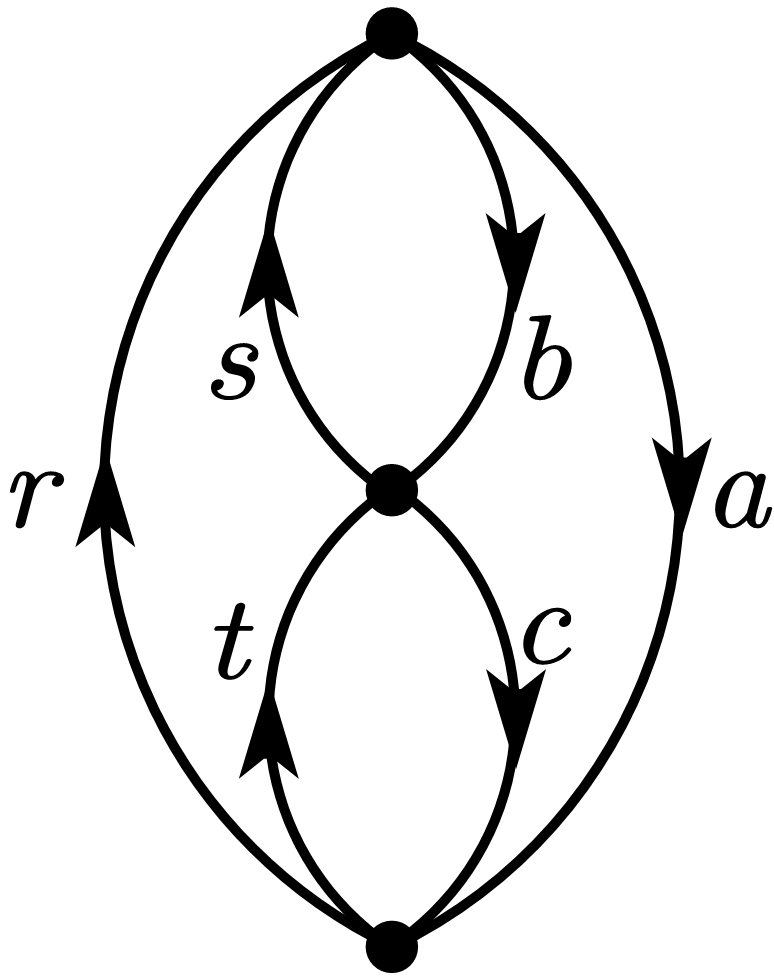
\includegraphics[scale=1.0,trim=0 -4 0 -4]{./pictures/6.12/hugenholtz_3.png}
		\end{minipage}
		
	\end{tabular}
	\captionof{figure}{All third-order Hugenholtz diagrams.}\label{fig:exe12_1}
	\end{center}
	
	In fact, the ``pushing together" results of these third-order Goldstone diagrams in the table 6.2 can be summarized as follows.
	\begin{itemize}
	
	\item Pushing together the second or the seventh third-order Goldstone diagrams leads to the first Hugenholtz diagram.
	
	\item Pushing together the first and the eighth third-order Goldstone diagrams leads to the second Hugenholtz diagram.
	
	\item Pushing together the rest of third-order Goldstone diagrams leads to the third Hugenholtz diagram.
	
	\end{itemize}
	
	Firstly, we will verify that the sum of the second and the seventh third-order Goldstone diagrams is the first third-order Hugenholtz diagram. The sum of the second and the seventh third-order Goldstone diagrams is
	\begin{align*}
		&\hspace{1.4em} (-1)^{4+2} \left( \frac{1}{2} \right) \sum_{abcdrs} \frac{ \langle ad | rs \rangle \langle cb | ad \rangle \langle rs | cb \rangle }{ ( \varepsilon_a + \varepsilon_d - \varepsilon_r - \varepsilon_s ) ( \varepsilon_c + \varepsilon_b - \varepsilon_r - \varepsilon_s ) } \\
		&\hspace{6em} + (-1)^{4+1} \left( \frac{1}{2} \right) \sum_{abcdrs} \frac{ \langle ac | rs \rangle \langle db | ac \rangle \langle sr | db \rangle }{ ( \varepsilon_a + \varepsilon_c - \varepsilon_r - \varepsilon_s ) ( \varepsilon_d + \varepsilon_b - \varepsilon_r - \varepsilon_s ) } \\
		&= \frac{1}{2} \sum_{abcdrs} \frac{ \langle ad | rs \rangle \langle cb | ad \rangle \langle rs | cb \rangle }{ ( \varepsilon_a + \varepsilon_d - \varepsilon_r - \varepsilon_s ) ( \varepsilon_c + \varepsilon_b - \varepsilon_r - \varepsilon_s ) } - \frac{ \langle ad | rs \rangle \langle cb | ad \rangle \langle sr | cb \rangle }{ ( \varepsilon_a + \varepsilon_d - \varepsilon_r - \varepsilon_s ) ( \varepsilon_c + \varepsilon_b - \varepsilon_r - \varepsilon_s ) } \\
		&= \frac{1}{2} \sum_{abcdrs} \frac{ \langle ad | rs \rangle \langle cb | ad \rangle \left( \langle rs | cb \rangle - \langle sr | cb \rangle \right) }{ ( \varepsilon_a + \varepsilon_d - \varepsilon_r - \varepsilon_s ) ( \varepsilon_c + \varepsilon_b - \varepsilon_r - \varepsilon_s ) } = \frac{1}{2} \sum_{abcdrs} \frac{ \langle ab | rs \rangle \langle cd | ab \rangle \left( \langle rs | cd \rangle - \langle sr | cd \rangle \right) }{ ( \varepsilon_a + \varepsilon_b - \varepsilon_r - \varepsilon_s ) ( \varepsilon_c + \varepsilon_d - \varepsilon_r - \varepsilon_s ) },
	\end{align*}
	and the first Hugenholtz diagram can be simplified to
	\begin{align*}
		&\hspace{1.4em} \frac{1}{8} \sum_{abcdrs} \frac{ \langle ab || rs \rangle \langle rs || cd \rangle \langle cd || ab \rangle }{ ( \varepsilon_a + \varepsilon_b - \varepsilon_r - \varepsilon_s ) ( \varepsilon_c + \varepsilon_d - \varepsilon_r - \varepsilon_s ) } \\
		&= \frac{1}{8} \sum_{abcdrs} \frac{ ( \langle ab | rs \rangle - \langle ab | sr \rangle )( \langle rs | cd \rangle - \langle rs | dc \rangle ) ( \langle cd | ab \rangle - \langle cd | ba \rangle ) }{ ( \varepsilon_a + \varepsilon_b - \varepsilon_r - \varepsilon_s ) ( \varepsilon_c + \varepsilon_d - \varepsilon_r - \varepsilon_s ) } \\
		&= \frac{1}{8} \sum_{abcdrs} \frac{ \langle ab | rs \rangle \langle rs | cd \rangle \langle cd | ab \rangle }{ ( \varepsilon_a + \varepsilon_b - \varepsilon_r - \varepsilon_s ) ( \varepsilon_c + \varepsilon_d - \varepsilon_r - \varepsilon_s ) } - \frac{ \langle ab | rs \rangle \langle rs | cd \rangle \langle cd | ba \rangle }{ ( \varepsilon_a + \varepsilon_b - \varepsilon_r - \varepsilon_s ) ( \varepsilon_c + \varepsilon_d - \varepsilon_r - \varepsilon_s ) } \\
		&\hspace{6em} - \frac{ \langle ab | rs \rangle \langle rs | dc \rangle \langle cd | ab \rangle }{ ( \varepsilon_a + \varepsilon_b - \varepsilon_r - \varepsilon_s ) ( \varepsilon_c + \varepsilon_d - \varepsilon_r - \varepsilon_s ) } + \frac{ \langle ab | rs \rangle \langle rs | dc \rangle \langle cd | ba \rangle }{ ( \varepsilon_a + \varepsilon_b - \varepsilon_r - \varepsilon_s ) ( \varepsilon_c + \varepsilon_d - \varepsilon_r - \varepsilon_s ) } \\
		&\hspace{6em} - \frac{ \langle ab | sr \rangle \langle rs | cd \rangle \langle cd | ab \rangle }{ ( \varepsilon_a + \varepsilon_b - \varepsilon_r - \varepsilon_s ) ( \varepsilon_c + \varepsilon_d - \varepsilon_r - \varepsilon_s ) } + \frac{ \langle ab | sr \rangle \langle rs | cd \rangle \langle cd | ba \rangle }{ ( \varepsilon_a + \varepsilon_b - \varepsilon_r - \varepsilon_s ) ( \varepsilon_c + \varepsilon_d - \varepsilon_r - \varepsilon_s ) } \\
		&\hspace{6em} + \frac{ \langle ab | sr \rangle \langle rs | dc \rangle \langle cd | ab \rangle }{ ( \varepsilon_a + \varepsilon_b - \varepsilon_r - \varepsilon_s ) ( \varepsilon_c + \varepsilon_d - \varepsilon_r - \varepsilon_s ) } - \frac{ \langle ab | sr \rangle \langle rs | dc \rangle \langle cd | ba \rangle }{ ( \varepsilon_a + \varepsilon_b - \varepsilon_r - \varepsilon_s ) ( \varepsilon_c + \varepsilon_d - \varepsilon_r - \varepsilon_s ) } \\
		&= \frac{1}{8} \sum_{abcdrs} \frac{ \langle ab | rs \rangle \langle cd | ab \rangle \langle rs | cd \rangle }{ ( \varepsilon_a + \varepsilon_b - \varepsilon_r - \varepsilon_s ) ( \varepsilon_c + \varepsilon_d - \varepsilon_r - \varepsilon_s ) } - \frac{ \langle ab | rs \rangle \langle rs | dc \rangle \langle dc | ba \rangle }{ ( \varepsilon_a + \varepsilon_b - \varepsilon_r - \varepsilon_s ) ( \varepsilon_c + \varepsilon_d - \varepsilon_r - \varepsilon_s ) } \\
		&\hspace{6em} - \frac{ \langle ab | rs \rangle \langle sr | cd \rangle \langle cd | ab \rangle }{ ( \varepsilon_a + \varepsilon_b - \varepsilon_r - \varepsilon_s ) ( \varepsilon_c + \varepsilon_d - \varepsilon_r - \varepsilon_s ) } + \frac{ \langle ab | rs \rangle \langle sr | dc \rangle \langle dc | ba \rangle }{ ( \varepsilon_a + \varepsilon_b - \varepsilon_r - \varepsilon_s ) ( \varepsilon_c + \varepsilon_d - \varepsilon_r - \varepsilon_s ) } \\
		&\hspace{6em} - \frac{ \langle ab | rs \rangle \langle sr | cd \rangle \langle cd | ab \rangle }{ ( \varepsilon_a + \varepsilon_b - \varepsilon_r - \varepsilon_s ) ( \varepsilon_c + \varepsilon_d - \varepsilon_r - \varepsilon_s ) } + \frac{ \langle ab | rs \rangle \langle sr | dc \rangle \langle dc | ba \rangle }{ ( \varepsilon_a + \varepsilon_b - \varepsilon_r - \varepsilon_s ) ( \varepsilon_c + \varepsilon_d - \varepsilon_r - \varepsilon_s ) } \\
		&\hspace{6em} + \frac{ \langle ab | rs \rangle \langle sr | dc \rangle \langle cd | ab \rangle }{ ( \varepsilon_a + \varepsilon_b - \varepsilon_r - \varepsilon_s ) ( \varepsilon_c + \varepsilon_d - \varepsilon_r - \varepsilon_s ) } - \frac{ \langle ab | rs \rangle \langle sr | cd \rangle \langle dc | ba \rangle }{ ( \varepsilon_a + \varepsilon_b - \varepsilon_r - \varepsilon_s ) ( \varepsilon_c + \varepsilon_d - \varepsilon_r - \varepsilon_s ) } \\
		&= \frac{1}{2} \sum_{abcdrs} \frac{ \langle ab | rs \rangle \langle cd | ab \rangle \left( \langle rs | cd \rangle - \langle sr | cd \rangle \right) }{ ( \varepsilon_a + \varepsilon_b - \varepsilon_r - \varepsilon_s ) ( \varepsilon_c + \varepsilon_d - \varepsilon_r - \varepsilon_s ) }.
	\end{align*}
	Thus, we have verified that the sum of the second and the seventh third-order Goldstone diagrams is the first third-order Hugenholtz diagram.
	
	Secondly, we will verify that the sum of the first and the eighth third-order Goldstone diagrams is the second third-order Hugenholtz diagram. The sum of the first and the eighth third-order Goldstone diagrams is
	\begin{align*}
		&(-1)^{2+2} \left( \frac{1}{2} \right) \sum_{abrsut} \frac{ \langle ab | ru \rangle \langle ru | ts \rangle \langle ts | ab \rangle }{ ( \varepsilon_a + \varepsilon_b - \varepsilon_r - \varepsilon_u ) ( \varepsilon_a + \varepsilon_b - \varepsilon_t - \varepsilon_s ) } \\
		&\hspace{6em}+ (-1)^{2+1} \left( \frac{1}{2} \right) \sum_{abrsut} \frac{ \langle ab | rt \rangle \langle tr | us \rangle \langle us | ab \rangle }{ ( \varepsilon_a + \varepsilon_b - \varepsilon_t - \varepsilon_r ) ( \varepsilon_a + \varepsilon_b - \varepsilon_u - \varepsilon_s ) } \\
		&= \frac{1}{2} \sum_{abrsut} \frac{ \langle ab | ru \rangle \langle ru | ts \rangle \langle ts | ab \rangle }{ ( \varepsilon_a + \varepsilon_b - \varepsilon_r - \varepsilon_u ) ( \varepsilon_a + \varepsilon_b - \varepsilon_t - \varepsilon_s ) } - \frac{ \langle ab | ru \rangle \langle ur | ts \rangle \langle ts | ab \rangle }{ ( \varepsilon_a + \varepsilon_b - \varepsilon_u - \varepsilon_r ) ( \varepsilon_a + \varepsilon_b - \varepsilon_t - \varepsilon_s ) } \\
		&= \frac{1}{2} \sum_{abrsut} \frac{ \langle ab | ru \rangle \langle ts | ab \rangle ( \langle ru | ts \rangle - \langle ur | ts \rangle ) }{ ( \varepsilon_a + \varepsilon_b - \varepsilon_r - \varepsilon_u ) ( \varepsilon_a + \varepsilon_b - \varepsilon_t - \varepsilon_s ) } = \frac{1}{2} \sum_{abrsut} \frac{ \langle ab | rs \rangle \langle tu | ab \rangle ( \langle rs | tu \rangle - \langle sr | tu \rangle ) }{ ( \varepsilon_a + \varepsilon_b - \varepsilon_r - \varepsilon_s ) ( \varepsilon_a + \varepsilon_b - \varepsilon_t - \varepsilon_u ) }.
	\end{align*}
	and the second Hugenholtz diagram can be simplified to
	\begin{align*}
		&\hspace{1.4em} \frac{1}{8} \sum_{abrstu} \frac{ \langle ab || rs \rangle \langle rs || tu \rangle \langle tu || ab \rangle }{ ( \varepsilon_a + \varepsilon_b - \varepsilon_r - \varepsilon_s ) ( \varepsilon_a + \varepsilon_b - \varepsilon_t - \varepsilon_u ) } \\
		&= \frac{1}{8} \sum_{abrstu} \frac{ ( \langle ab | rs \rangle - \langle ab | sr \rangle )( \langle rs | tu \rangle - \langle rs | ut \rangle ) ( \langle tu | ab \rangle - \langle tu | ba \rangle ) }{ ( \varepsilon_a + \varepsilon_b - \varepsilon_r - \varepsilon_s ) ( \varepsilon_a + \varepsilon_b - \varepsilon_t - \varepsilon_u ) } \\
		&= \frac{1}{8} \sum_{abrstu} \frac{ \langle ab | rs \rangle \langle rs | tu \rangle \langle tu | ab \rangle }{ ( \varepsilon_a + \varepsilon_b - \varepsilon_r - \varepsilon_s ) ( \varepsilon_a + \varepsilon_b - \varepsilon_t - \varepsilon_u ) } - \frac{ \langle ab | rs \rangle \langle rs | tu \rangle \langle tu | ba \rangle }{ ( \varepsilon_a + \varepsilon_b - \varepsilon_r - \varepsilon_s ) ( \varepsilon_a + \varepsilon_b - \varepsilon_t - \varepsilon_u ) } \\
		&\hspace{6em} - \frac{ \langle ab | rs \rangle \langle rs | ut \rangle \langle tu | ab \rangle }{ ( \varepsilon_a + \varepsilon_b - \varepsilon_r - \varepsilon_s ) ( \varepsilon_a + \varepsilon_b - \varepsilon_t - \varepsilon_u ) } + \frac{ \langle ab | rs \rangle \langle rs | ut \rangle \langle tu | ba \rangle }{ ( \varepsilon_a + \varepsilon_b - \varepsilon_r - \varepsilon_s ) ( \varepsilon_a + \varepsilon_b - \varepsilon_t - \varepsilon_u ) } \\
		&\hspace{6em} - \frac{ \langle ab | sr \rangle \langle rs | tu \rangle \langle tu | ab \rangle }{ ( \varepsilon_a + \varepsilon_b - \varepsilon_r - \varepsilon_s ) ( \varepsilon_a + \varepsilon_b - \varepsilon_t - \varepsilon_u ) } + \frac{ \langle ab | sr \rangle \langle rs | tu \rangle \langle tu | ba \rangle }{ ( \varepsilon_a + \varepsilon_b - \varepsilon_r - \varepsilon_s ) ( \varepsilon_a + \varepsilon_b - \varepsilon_t - \varepsilon_u ) } \\
		&\hspace{6em} + \frac{ \langle ab | sr \rangle \langle rs | ut \rangle \langle tu | ab \rangle }{ ( \varepsilon_a + \varepsilon_b - \varepsilon_r - \varepsilon_s ) ( \varepsilon_a + \varepsilon_b - \varepsilon_t - \varepsilon_u ) } - \frac{ \langle ab | sr \rangle \langle rs | ut \rangle \langle tu | ba \rangle }{ ( \varepsilon_a + \varepsilon_b - \varepsilon_r - \varepsilon_s ) ( \varepsilon_a + \varepsilon_b - \varepsilon_t - \varepsilon_u ) } \\
		&= \frac{1}{8} \sum_{abrstu} \frac{ \langle ab | rs \rangle \langle rs | tu \rangle \langle tu | ab \rangle }{ ( \varepsilon_a + \varepsilon_b - \varepsilon_r - \varepsilon_s ) ( \varepsilon_a + \varepsilon_b - \varepsilon_t - \varepsilon_u ) } - \frac{ \langle ab | rs \rangle \langle rs | ut \rangle \langle ut | ba \rangle }{ ( \varepsilon_a + \varepsilon_b - \varepsilon_r - \varepsilon_s ) ( \varepsilon_a + \varepsilon_b - \varepsilon_t - \varepsilon_u ) } \\
		&\hspace{6em} - \frac{ \langle ab | rs \rangle \langle rs | tu \rangle \langle ut | ab \rangle }{ ( \varepsilon_a + \varepsilon_b - \varepsilon_r - \varepsilon_s ) ( \varepsilon_a + \varepsilon_b - \varepsilon_t - \varepsilon_u ) } + \frac{ \langle ab | rs \rangle \langle rs | tu \rangle \langle ut | ba \rangle }{ ( \varepsilon_a + \varepsilon_b - \varepsilon_r - \varepsilon_s ) ( \varepsilon_a + \varepsilon_b - \varepsilon_t - \varepsilon_u ) } \\
		&\hspace{6em} - \frac{ \langle ab | rs \rangle \langle sr | tu \rangle \langle tu | ab \rangle }{ ( \varepsilon_a + \varepsilon_b - \varepsilon_r - \varepsilon_s ) ( \varepsilon_a + \varepsilon_b - \varepsilon_t - \varepsilon_u ) } + \frac{ \langle ab | rs \rangle \langle sr | ut \rangle \langle ut | ba \rangle }{ ( \varepsilon_a + \varepsilon_b - \varepsilon_r - \varepsilon_s ) ( \varepsilon_a + \varepsilon_b - \varepsilon_t - \varepsilon_u ) } \\
		&\hspace{6em} + \frac{ \langle ab | rs \rangle \langle sr | ut \rangle \langle tu | ab \rangle }{ ( \varepsilon_a + \varepsilon_b - \varepsilon_r - \varepsilon_s ) ( \varepsilon_a + \varepsilon_b - \varepsilon_t - \varepsilon_u ) } - \frac{ \langle ab | rs \rangle \langle sr | tu \rangle \langle ut | ba \rangle }{ ( \varepsilon_a + \varepsilon_b - \varepsilon_r - \varepsilon_s ) ( \varepsilon_a + \varepsilon_b - \varepsilon_t - \varepsilon_u ) } \\
		&= \frac{1}{2} \sum_{abrstu} \frac{ \langle ab | rs \rangle \langle rs | tu \rangle \langle tu | ab \rangle }{ ( \varepsilon_a + \varepsilon_b - \varepsilon_r - \varepsilon_s ) ( \varepsilon_a + \varepsilon_b - \varepsilon_t - \varepsilon_u ) } - \frac{ \langle ab | rs \rangle \langle rs | ut \rangle \langle ut | ba \rangle }{ ( \varepsilon_a + \varepsilon_b - \varepsilon_r - \varepsilon_s ) ( \varepsilon_a + \varepsilon_b - \varepsilon_t - \varepsilon_u ) } \\
		&= \frac{1}{2} \sum_{abrsut} \frac{ \langle ab | rs \rangle \langle tu | ab \rangle ( \langle rs | tu \rangle - \langle sr | tu \rangle ) }{ ( \varepsilon_a + \varepsilon_b - \varepsilon_r - \varepsilon_s ) ( \varepsilon_a + \varepsilon_b - \varepsilon_t - \varepsilon_u ) }.
	\end{align*}
	Thus, we have verified that the sum of the first and the eighth third-order Goldstone diagrams is the second third-order Hugenholtz diagram.
	
	Thirdly, we will verify that the sum of the rest of third-order Goldstone diagrams is the third third-order Hugenholtz diagram. The third third-order Hugenholtz diagram is	
	\begin{align*}
		&\hspace{1.4em}\sum_{abcrst} \frac{ \langle ab || rs \rangle \langle cs || tb \rangle \langle rt || ac \rangle }{ ( \varepsilon_a + \varepsilon_b - \varepsilon_s - \varepsilon_r ) ( \varepsilon_a + \varepsilon_c - \varepsilon_r - \varepsilon_t ) } \\
		&= \sum_{abcrst} \frac{ [ \langle ab | rs \rangle - \langle ab | sr \rangle ] [ \langle cs | tb \rangle - \langle cs | bt \rangle ] [ \langle rt | ac \rangle - \langle rt | ca \rangle ] }{ ( \varepsilon_a + \varepsilon_b - \varepsilon_s - \varepsilon_r ) ( \varepsilon_a + \varepsilon_c - \varepsilon_r - \varepsilon_t ) } \\
		&= \sum_{abcrst} \frac{ \langle ab | rs \rangle \langle cs | tb \rangle \langle rt | ac \rangle }{ ( \varepsilon_a + \varepsilon_b - \varepsilon_r - \varepsilon_s ) ( \varepsilon_a + \varepsilon_c - \varepsilon_r - \varepsilon_t ) } - \frac{ \langle ab | rs \rangle \langle cs | tb \rangle \langle rt | ca \rangle }{ ( \varepsilon_a + \varepsilon_b - \varepsilon_r - \varepsilon_s ) ( \varepsilon_a + \varepsilon_c - \varepsilon_r - \varepsilon_t ) } \\
		&\hspace{4em} - \frac{ \langle ab | rs \rangle \langle cs | bt \rangle \langle rt | ac \rangle }{ ( \varepsilon_a + \varepsilon_b - \varepsilon_r - \varepsilon_s ) ( \varepsilon_a + \varepsilon_c - \varepsilon_r - \varepsilon_t ) } + \frac{ \langle ab | rs \rangle \langle cs | bt \rangle \langle rt | ca \rangle }{ ( \varepsilon_a + \varepsilon_b - \varepsilon_r - \varepsilon_s ) ( \varepsilon_a + \varepsilon_c - \varepsilon_r - \varepsilon_t ) } \\
		&\hspace{4em} - \frac{ \langle ab | sr \rangle \langle cs | tb \rangle \langle rt | ac \rangle }{ ( \varepsilon_a + \varepsilon_b - \varepsilon_r - \varepsilon_s ) ( \varepsilon_a + \varepsilon_c - \varepsilon_r - \varepsilon_t ) } + \frac{ \langle ab | sr \rangle \langle cs | tb \rangle \langle rt | ca \rangle }{ ( \varepsilon_a + \varepsilon_b - \varepsilon_r - \varepsilon_s ) ( \varepsilon_a + \varepsilon_c - \varepsilon_r - \varepsilon_t ) } \\
		&\hspace{4em} + \frac{ \langle ab | sr \rangle \langle cs | bt \rangle \langle rt | ac \rangle }{ ( \varepsilon_a + \varepsilon_b - \varepsilon_r - \varepsilon_s ) ( \varepsilon_a + \varepsilon_c - \varepsilon_r - \varepsilon_t ) } - \frac{ \langle ab | sr \rangle \langle cs | bt \rangle \langle rt | ca \rangle }{ ( \varepsilon_a + \varepsilon_b - \varepsilon_r - \varepsilon_s ) ( \varepsilon_a + \varepsilon_c - \varepsilon_r - \varepsilon_t ) } \\
		&= \sum_{abcrst} \frac{ \langle ac | rt \rangle \langle bt | sc \rangle \langle rs | ab \rangle }{ ( \varepsilon_a + \varepsilon_c - \varepsilon_r - \varepsilon_t ) ( \varepsilon_a + \varepsilon_b - \varepsilon_r - \varepsilon_s ) } - \frac{ \langle bc | rt \rangle \langle at | sc \rangle \langle rs | ab \rangle }{ ( \varepsilon_b + \varepsilon_c - \varepsilon_t - \varepsilon_r ) ( \varepsilon_a + \varepsilon_b - \varepsilon_r - \varepsilon_s ) } \\
		&\hspace{2em} - \sum_{abcrst} \frac{ \langle bc | rt \rangle \langle ra | sb \rangle \langle st | ac \rangle }{ ( \varepsilon_b + \varepsilon_c - \varepsilon_r - \varepsilon_t ) ( \varepsilon_a + \varepsilon_c - \varepsilon_s - \varepsilon_t ) } + \sum_{abcrst} \frac{ \langle bc | rt \rangle \langle ar | bs \rangle \langle ts | ac \rangle }{ ( \varepsilon_c + \varepsilon_b - \varepsilon_r - \varepsilon_t ) ( \varepsilon_a + \varepsilon_c - \varepsilon_s - \varepsilon_t ) } \\
		&\hspace{2em} - \sum_{abcrst} \frac{ \langle ab | rs \rangle \langle sc | at \rangle \langle rt | bc \rangle }{ ( \varepsilon_a + \varepsilon_b - \varepsilon_r - \varepsilon_s ) ( \varepsilon_c + \varepsilon_b - \varepsilon_r - \varepsilon_t ) } + \sum_{abcrst} \frac{ \langle cb | rt \rangle \langle at | sc \rangle \langle rs | ab \rangle }{ ( \varepsilon_c + \varepsilon_b - \varepsilon_r - \varepsilon_t ) ( \varepsilon_a + \varepsilon_b - \varepsilon_r - \varepsilon_s ) } \\
		&\hspace{2em} + \sum_{abcrst} \frac{ \langle cb | rt \rangle \langle ra | sb \rangle \langle st | ac \rangle }{ ( \varepsilon_c + \varepsilon_b - \varepsilon_r - \varepsilon_t ) ( \varepsilon_a + \varepsilon_c - \varepsilon_s - \varepsilon_t ) } - \sum_{abcrst} \frac{ \langle ac | rt \rangle \langle rb | sc \rangle \langle st | ab \rangle }{ ( \varepsilon_a + \varepsilon_c - \varepsilon_r - \varepsilon_t ) ( \varepsilon_a + \varepsilon_b - \varepsilon_s - \varepsilon_t ) }.
	\end{align*}	
	These eight terms correspond to the fifth, twelfth, fourth, ninth, eleventh, sixth, tenth, third third-order Goldstone diagrams, respectively.
	
	In conclusion, we have verified that the first third-order Hugenholtz diagram corresponds the second and the seventh third-order Goldstone diagrams, the second third-order Hugenholtz diagram corresponds the first and the eighth third-order Goldstone diagrams, and the third third-order Hugenholtz diagram corresponds the third, fourth, fifth, sixth, ninth, tenth, eleventh, twelfth third-order Goldstone diagrams.
	\end{solution}
	
	\subsection{Summation of Diagrams}
	
	\subsection{What Is the Linked Cluster Theorem?}
	
	% 6.13
	\begin{exercise}
	Calculate $E^{(3)}_0$ for a supermolecule consisting of $N$ non-interacting minimal basis $\ce{H2}$ molecules by evaluating the Goldstone diagrams in Table 6.2. Compare your result with that of Eq.(6.92), which was obtained algebraically by explicitly cancelling terms proportional to $N^2$.
	
	{\it Hint}: Simply show that the value of each Goldstone diagram for the supermolecule in $N$ times the result for a single molecule.
	\end{exercise}
	
	\begin{solution}
	Note that in this model, all two-electron integrals involving orbitals from different units are zero, and all third-order terms in the table 6.2 will be zero unless their numerators are non-zero. Thus, each third-order term of this model is just the sum of that of each units, leading that the value of each Goldstone diagram for the supermolecule in $N$ times the result for a single molecule.
	\end{solution}
	
	\section{Some Illustrative Calculations}

\end{document}
